% ============================================================================
%  《Between Electric-Magnetic Duality and the Langlands Program》中译本
%  主文件：请用 XeLaTeX 编译两次
%      xelatex main.tex
%      xelatex main.tex
% ============================================================================
% ============================================================================
%  《Between Electric-Magnetic Duality and the Langlands Program》中译本
%  原书：David Ben-Zvi 教授 2021 年春季 UT Austin 课程讲义
%        笔记：Jackson Van Dyke
%  排版：XeLaTeX（请连续编译两遍以生成目录与交叉引用）
% ============================================================================
\documentclass[UTF8,11pt,a4paper,fontset=windows]{ctexbook}

% ---------- 页面与版式 ----------
\usepackage{geometry}
\geometry{left=2.55cm,right=2.55cm,top=2.55cm,bottom=2.6cm,headsep=0.5cm,footskip=1.1cm}
\usepackage{fancyhdr}
\usepackage{xcolor}
\usepackage{graphicx}
\usepackage{amsmath,amssymb}
\usepackage{amsthm}
\usepackage{caption}
\captionsetup{font=small,labelfont=bf,labelsep=quad}
\usepackage{booktabs}
\usepackage{array}
\usepackage{longtable}

% ---------- 超链接 ----------
\usepackage[unicode,bookmarksnumbered=true,breaklinks=true,
            colorlinks=true,linkcolor=blue!45!black,citecolor=blue!45!black,
            urlcolor=blue!45!black]{hyperref}
\hypersetup{
  pdftitle={电磁对偶与 Langlands 纲领之间（中译本·学术注疏版）},
  pdfauthor={David Ben-Zvi（讲义）；Jackson Van Dyke（笔记）；DeepSeek 学术助手（中译与注疏）},
  pdfsubject={几何 Langlands 纲领、电磁对偶、拓扑场论},
  pdfkeywords={Langlands program, electric-magnetic duality, TFT, gauge theory}
}

% ---------- 行距与段落 ----------
\linespread{1.18}
\setlength{\parskip}{0.25em}
\setlength{\parindent}{2em}
\setlength{\emergencystretch}{3em}

% ---------- 章节标题样式 ----------
\ctexset{
  chapter = {
    name = {第,章},
    number = \arabic{chapter},
    format = \Large\bfseries\centering,
    beforeskip = 8pt,
    afterskip = 18pt,
  },
  section = {
    format = \large\bfseries\raggedright,
    beforeskip = 14pt,
    afterskip = 6pt,
  },
  subsection = {
    format = \normalsize\bfseries\raggedright,
    beforeskip = 10pt,
    afterskip = 4pt,
  },
}

% ---------- 页眉页脚 ----------
\pagestyle{fancy}
\fancyhf{}
\fancyhead[LE]{\small\thepage}
\fancyhead[RO]{\small\thepage}
\fancyhead[LO]{\small\nouppercase{\leftmark}}
\fancyhead[RE]{\small\nouppercase{\rightmark}}
\renewcommand{\headrulewidth}{0.3pt}
\fancypagestyle{plain}{\fancyhf{}\fancyfoot[C]{\small\thepage}\renewcommand{\headrulewidth}{0pt}}

% ---------- 图片搜索路径 ----------
\graphicspath{{figures/}{figures/inline/}{./}}

% ---------- 术语宏 ----------
% 首次出现时使用：\term{中文译名}{English term}
\newcommand{\term}[2]{#1（#2）}
% 保留英文原词
\newcommand{\eng}[1]{\textit{#1}}

% ---------- 内嵌示意图 ----------
% 用法：\diagram[0.25\textwidth]{p135_d3.png}
\newcommand{\diagram}[2][0.28\textwidth]{%
  \begin{center}\includegraphics[width=#1]{#2}\end{center}}
% 带原文编号的图示方程：\diageq{10.13}{0.16\textwidth}{p135_d3.png}
\newcommand{\diageq}[3]{%
  \begin{equation}\tag{#1}\text{\includegraphics[width=#2]{#3}}\end{equation}}

% ---------- “本章重点” ----------
\newenvironment{keytakeaways}
  {\par\medskip\noindent
   \begin{minipage}{\linewidth}
   \hrule\vspace{5pt}\noindent\textbf{本章重点}\par\vspace{3pt}\small\noindent\ignorespaces}
  {\vspace{4pt}\hrule\end{minipage}\medskip}

% ---------- “本节要点” ----------
\newenvironment{sectionkey}
  {\par\smallskip\noindent
   \begin{minipage}{\linewidth}\small\noindent\textbf{本节要点：}\ignorespaces}
  {\end{minipage}\par\smallskip}

% ---------- 源文编号环境（保留原书编号） ----------
% 用法：\begin{srcdef}{3} ... \end{srcdef}
\newcommand{\srcenv}[3]{%
  \par\medskip\noindent\textbf{#1 #2.}\ \ignorespaces}
\newenvironment{srcdef}[1]{\par\medskip\noindent\textbf{定义 #1.}\ \ignorespaces}{\par\medskip}
\newenvironment{srcthm}[1]{\par\medskip\noindent\textbf{定理 #1.}\ \ignorespaces}{\par\medskip}
\newenvironment{srclem}[1]{\par\medskip\noindent\textbf{引理 #1.}\ \ignorespaces}{\par\medskip}
\newenvironment{srcprop}[1]{\par\medskip\noindent\textbf{命题 #1.}\ \ignorespaces}{\par\medskip}
\newenvironment{srccor}[1]{\par\medskip\noindent\textbf{推论 #1.}\ \ignorespaces}{\par\medskip}
\newenvironment{srcex}[1]{\par\medskip\noindent\textbf{例 #1.}\ \ignorespaces}{\par\medskip}
\newenvironment{srcrem}[1]{\par\medskip\noindent\textbf{注 #1.}\ \ignorespaces}{\par\medskip}
\newenvironment{srcconj}[1]{\par\medskip\noindent\textbf{猜想 #1.}\ \ignorespaces}{\par\medskip}
\newenvironment{srcclaim}[1]{\par\medskip\noindent\textbf{断言 #1.}\ \ignorespaces}{\par\medskip}
\newenvironment{srcnotation}[1]{\par\medskip\noindent\textbf{记号 #1.}\ \ignorespaces}{\par\medskip}

% ---------- 常用数学宏 ----------
\newcommand{\C}{\mathbb{C}}
\newcommand{\R}{\mathbb{R}}
\newcommand{\Z}{\mathbb{Z}}
\newcommand{\N}{\mathbb{N}}
\newcommand{\Q}{\mathbb{Q}}
\newcommand{\F}{\mathbb{F}}
\newcommand{\HH}{\mathbb{H}}
\newcommand{\GG}{\mathbb{G}}
\newcommand{\PP}{\mathbb{P}}
\newcommand{\bA}{\mathbb{A}}
\newcommand{\cO}{\mathcal{O}}
\newcommand{\cF}{\mathcal{F}}
\newcommand{\cG}{\mathcal{G}}
\newcommand{\cH}{\mathcal{H}}
\newcommand{\cC}{\mathcal{C}}
\newcommand{\cD}{\mathcal{D}}
\newcommand{\cA}{\mathcal{A}}
\newcommand{\cB}{\mathcal{B}}
\newcommand{\cL}{\mathcal{L}}
\newcommand{\cM}{\mathcal{M}}
\newcommand{\cN}{\mathcal{N}}
\newcommand{\cX}{\mathcal{X}}
\newcommand{\cZ}{\mathcal{Z}}
\newcommand{\fg}{\mathfrak{g}}
\renewcommand{\proofname}{证明}
\newcommand{\sph}{\mathrm{Sph}}
\newcommand{\Bun}{\mathrm{Bun}}
\newcommand{\Loc}{\mathrm{Loc}}
\newcommand{\Rep}{\mathrm{Rep}}
\newcommand{\Vect}{\mathrm{Vect}}
\newcommand{\Shv}{\mathrm{Shv}}
\newcommand{\End}{\mathrm{End}}
\newcommand{\Hom}{\mathrm{Hom}}
\newcommand{\Aut}{\mathrm{Aut}}
\newcommand{\Spec}{\mathrm{Spec}}
\newcommand{\Gal}{\mathrm{Gal}}
\newcommand{\Gr}{\mathrm{Gr}}
\newcommand{\QC}{\mathrm{QC}}
\newcommand{\IndCoh}{\mathrm{IndCoh}}
\newcommand{\Bord}{\mathrm{Bord}}
\newcommand{\Pic}{\mathrm{Pic}}
\newcommand{\Jac}{\mathrm{Jac}}
\newcommand{\G}{\mathbb{G}}
\newcommand{\cE}{\mathcal{E}}
\newcommand{\cP}{\mathcal{P}}
\newcommand{\Sph}{\mathrm{Sph}}
\newcommand{\GL}{\mathrm{GL}}
\newcommand{\SL}{\mathrm{SL}}
\newcommand{\PSL}{\mathrm{PSL}}
\newcommand{\PGL}{\mathrm{PGL}}
\newcommand{\Sp}{\mathrm{Sp}}
\newcommand{\SO}{\mathrm{SO}}
\newcommand{\LG}{\mathrm{LG}}

% ---------- 图表标题前缀 ----------
\renewcommand{\figurename}{图}
\renewcommand{\tablename}{表}
\renewcommand{\contentsname}{目\quad 录}
\renewcommand{\bibname}{参考文献}

% ---------- 微调 ----------
\allowdisplaybreaks[2]
\setlength{\abovedisplayskip}{6pt}
\setlength{\belowdisplayskip}{6pt}


\begin{document}

% ---------------------------------------------------------------------------
% 封面
% ---------------------------------------------------------------------------
\begin{titlepage}
  \vspace*{2.2cm}
  \begin{center}
    {\LARGE\bfseries 电磁对偶与 Langlands 纲领之间}\\[0.8cm]
    {\large\itshape Between Electric-Magnetic Duality\\[0.15cm]
      and the Langlands Program}\\[1.6cm]
    {\Large David Ben-Zvi}\\[0.35cm]
    {\normalsize 2021 年春季学期，德克萨斯大学奥斯汀分校（UT Austin）课程讲义}\\[0.25cm]
    {\normalsize 笔记：Jackson Van Dyke}\\[2.2cm]
    {\Large\bfseries 中译本 · 学术注疏版}\\[0.5cm]
    {\normalsize 术语审校、公式复核与译者注：DeepSeek 学术助手}\\[0.2cm]
    {\normalsize 2026 年}
  \end{center}
\end{titlepage}

\frontmatter

% ---------------------------------------------------------------------------
% 译者说明
% ---------------------------------------------------------------------------
\chapter*{译者说明}
\addcontentsline{toc}{chapter}{译者说明}
\markboth{译者说明}{译者说明}

\noindent\textbf{一、关于本书的作者与性质。}
摆在读者面前的这份文献，题为《Between Electric-Magnetic Duality and the Langlands
Program》，是 \textbf{David Ben-Zvi} 教授 2021 年春季在德克萨斯大学奥斯汀分校
（UT Austin）讲授的几何 Langlands 课程讲义，由 \textbf{Jackson Van Dyke} 现场记录整理，
共 17 章、304 页。它不是 Edward Witten 的论文：Witten 与 Anton Kapustin 2007 年的长文
\textit{Electric-Magnetic Duality and the Geometric Langlands Program} 是本书反复引用的
思想源头（见参考文献 \texttt{[KW07]}），但本书的作者与文体均属 Ben-Zvi 的讲义传统。
读者若因书名而误以为它是 Witten 的手笔，请以本说明为准。

\noindent\textbf{二、翻译原则。}
\begin{enumerate}
  \item \textbf{逐段全译。} 正文、脚注、括号补充、讲次日期均保留；不概括、不节译、不补写原文没有的物理内容。
  \item \textbf{公式保真。} 所有公式按原 PDF 逐符号重排，保留原书编号（如 (10.13)），
        多行公式用 \texttt{align} 并逐行编号；上下标、花体、对偶群记号 $G^{\vee}$ 等一律照原样。
  \item \textbf{术语统一。} 以中文学界通行译法为准，首次出现时以“中文（English）”形式给出；
        人名、群名、定理名保留英文。主要术语见附录 B。
  \item \textbf{图表剥离。} 原 PDF 中 27 幅编号图、7 张表以及正文内大量交换图/配边图，
        均已按原位置裁剪为独立图片文件，并在译文中以 \texttt{figure} 环境或
        \texttt{\textbackslash diagram} 命令插入；图题译为中文并标注原页码。
        表格为保持原貌，原则上以图像保留（可后续重排）。
        图题、表题后所注“原文 p.~N”均指原 PDF 文件的第 N 页（含封面与目录，
        与书内印刷页码相差 1--2 页），以便读者按 PDF 阅读器页码直接定位。
  \item \textbf{审校批注。} 译者对推导易错处、作者略去的证明、记号冲突与原文笔误，
        以 \texttt{\% [Tutor Note: ...]} 的 LaTeX 注释形式就近标注，便于对照阅读；
        全部批注另汇编于附录 A，可单独查阅。
  \item \textbf{不掩盖错误。} 原书是现场笔记，作者本人也声明“likely to contain many errors”。
        凡发现疑似笔误，译文照译，并在批注中说明；译者不擅自改动正文而不加说明。
\end{enumerate}

\noindent\textbf{三、原文的已知缺陷。}
\begin{itemize}
  \item 原 PDF 第 151 页 Figure 10.4 只有图题、没有图形（页面留白），疑为原始稿件遗漏；
        译文保留图题并加注说明。
  \item 原 PDF 中部分页面带有听课者手写的橙色批注（如“fix fig. 10.4”），
        属于原始文献的一部分，译文以脚注或批注形式说明，不视为正文。
  \item 个别公式在 PDF 文本层存在字形错位（如括号被拆成 \texttt{\textbackslash x00}、
        \texttt{\textbackslash x01}），译文已按页面图像与上下文还原。
\end{itemize}

\noindent\textbf{四、编译方式。}
本源码使用 XeLaTeX 与 \texttt{ctexbook} 文档类，需连续编译两遍以生成目录与交叉引用：
\begin{center}
\texttt{xelatex main.tex}\quad\texttt{xelatex main.tex}
\end{center}
图片位于 \texttt{figures/} 与 \texttt{figures/inline/}，请保持相对路径不变。

\vspace{0.6cm}
\begin{flushright}
  译者\\[0.1cm]
  2026 年 10 月
\end{flushright}

\cleardoublepage

% ---------------------------------------------------------------------------
% 原笔记说明（译）
% ---------------------------------------------------------------------------
\chapter*{原笔记说明}
\addcontentsline{toc}{chapter}{原笔记说明}
\markboth{原笔记说明}{原笔记说明}

\begin{quote}
封面图：Rok Gregoric。

笔记：Jackson Van Dyke。这些笔记是现场记录的，因此很可能包含许多错误。
如有更正或疑问，请发邮件至 \texttt{[邮箱隐去]}。

感谢 Tom Gannon 发现并修正了一些错误。

Arun Debray 也在为同一门课程做笔记！
\end{quote}

\vspace{0.5cm}
\noindent（以上为原书第 2 页说明的译文。）

\cleardoublepage

% ---------------------------------------------------------------------------
% 目录
% ---------------------------------------------------------------------------
\tableofcontents
\cleardoublepage

\mainmatter

% ---------------------------------------------------------------------------
% 正文：各章由 book/chapters/chNN.tex 提供
% ---------------------------------------------------------------------------
% ============================================================================
%  第 1 章  概述
% ============================================================================
\chapter{概述}\label{ch:01}

\begin{flushright}
\small 第 1 讲；2021 年 1 月 19 日
\end{flushright}

\begin{keytakeaways}
本章给出全书的路线图。核心论点是：几何 Langlands 纲领应当被理解为一座连接数论与量子场论的桥梁，
更具体地说，是四维算术拓扑场论的两个对偶版本 $\mathcal{A}_G$ 与 $\mathcal{B}_{G^{\vee}}$ 之间的等价。
本章先回顾模形式/自守形式的经典图景：局部对称空间 $\Gamma\backslash G/K$ 上的 $L^2$ 谱理论、
Hecke 算子、周期与 Langlands 函子性；随后引入 Weil 的“罗塞塔石碑”，把数域、函数域与
Riemann 面放在同一张字典里，并说明为了容纳局部域与分歧数据，必须把字典升级为三维/四维的版本。
所使用的数学工具包括：约化群与算术格、局部对称空间、Hecke 代数、Galois 表示、局部系统与特征簇。
主要结论是式 \eqref{eq:1.34}：$\mathcal{A}_G\simeq\mathcal{B}_{G^{\vee}}$，它把自守侧的谱分解
与 Galois 侧的表示论组织成同一个 TFT 的两面。本章不含证明，只建立语言与直觉。
\end{keytakeaways}

\section{模形式/自守形式}
\begin{sectionkey}
本节把模形式与自守形式重新解释为局部对称空间上的谱问题：从 $\Gamma\backslash G/K$ 上的
$L^2$ 理论与双曲 Laplacian 出发，经 Eichler--Shimura 理论转入上同调；随后变动数域、
导子与 Hecke 算子，得到 Hilbert/Siegel 模形式、同余子群与 Hecke 本征值，最后以周期与
Langlands 函子性收束。核心图景是：自守形式是“基态”，Hecke 算子是守恒量，周期是测量。
\end{sectionkey}

\subsection{粗略想法}

模形式理论可以看成算术局部对称空间上的某种调和分析/量子力学。

局部对称空间的典型例子，是 $\mathrm{SL}_2(\Z)$ 作用在上半平面
$\mathbb{H}=\mathrm{SL}_2(\R)/\mathrm{SO}_2$ 上的基本域。换言之，我们考虑商空间
\begin{equation}\tag{1.1}\label{eq:1.1}
\mathcal{M}_{\mathrm{SL}_2\R}
  =\mathrm{SL}_2(\Z)\backslash\mathbb{H}
  =\mathrm{SL}_2(\Z)\backslash\mathrm{SL}_2(\R)/\mathrm{SO}_2 ,
\end{equation}
如图 \ref{fig:1-1} 所示。

对一般的约化代数群 $G$，可以考虑空间
\begin{equation}\tag{1.2}\label{eq:1.2}
\mathcal{M}_G=\Gamma\backslash G/K,
\end{equation}
其中 $\Gamma$ 是算术格，$K$ 是极大紧子群。眼下先限制在
\[
G=\mathrm{SL}_2(\R),\qquad
\Gamma=\mathrm{SL}_2(\Z),\qquad
K=\mathrm{SO}_2 .
\]
我们想在这个空间上做调和分析，也就是以有意义的方式分解其上的函数空间。在量子力学的情形，
我们主要关心 $L^2$ 函数：
\begin{equation}\tag{1.3}\label{eq:1.3}
L^2(\Gamma\backslash G/K),
\end{equation}
其上有双曲 Laplace 算子的作用。也就是说，我们要研究这个算子的谱理论。

同样的信息（或许以更易处理的形式）可以通过去掉 $K$ 得到。我们可以直接研究
\begin{equation}\tag{1.4}\label{eq:1.4}
\Gamma\backslash G=\mathrm{SL}_2(\Z)\backslash\mathrm{SL}_2(\R)
\end{equation}
上的 $L^2$ 函数；这是单位切丛，即前述空间上的一个圆丛。此时不再是研究 Laplacian，
而是利用齐性空间的结构研究整个 $\mathrm{SL}_2(\R)$ 的作用。

还可以把微分与多重微分纳入进来，即典范丛（的幂次）的截面：
\begin{equation}\tag{1.5}\label{eq:1.5}
\Gamma\bigl(\Gamma\backslash\mathbb{H},\,\omega^{k/2}\bigr).
\end{equation}

\begin{srcdef}{1}
$L^2(\Gamma\backslash G/K)$ 中的 $\Delta$-本征函数称为 \emph{Maass 形式}。
权为 $k$ 的模形式是 $\omega^{k/2}$ 的全纯截面。
\end{srcdef}

% [Tutor Note: 式 (1.5) 中的 $\omega^{k/2}$ 在 $k$ 为奇数时并不是通常意义下的线丛（需要 spin 结构，
%  或按自守因子的半整数权来理解）。作者在这里把“模形式 = 典范丛幂次的全纯截面”一笔带过，
%  严格处理需要引入覆盖群 $\mathrm{Mp}_2(\R)$ 或 metaplectic 结构；这是后续讨论半整数权模形式时的常见陷阱。]

\begin{srcrem}{1}
对拓扑学家而言，可能更愿意研究（拓扑）上同调（而不是微分形式），系数取某个局部系统
（即扭曲系数）。确实，模形式也可以来自 $\Gamma\backslash\mathbb{H}$ 的（扭曲）上同调，
这就是所谓的 \emph{Eichler--Shimura 理论}。

有人可能会担心，这样做离开了量子力学的世界；但转到上同调之后，我们做的其实是所谓的
\emph{拓扑量子力学}。相比“真正的”量子力学，本书会更关心前者。

这里的想法是：这个设定中没有动力学。我们只看基态，所以 Laplacian 为 $0$，只看调和的对象。
这确实与拓扑和上同调有关；而模形式正是某种基态。
\end{srcrem}

\begin{srcrem}{2}
如果取一般的 $G,K,\Gamma$，就得到更一般的\emph{自守形式}理论。
\end{srcrem}

\begin{figure}[htbp]
  \centering
  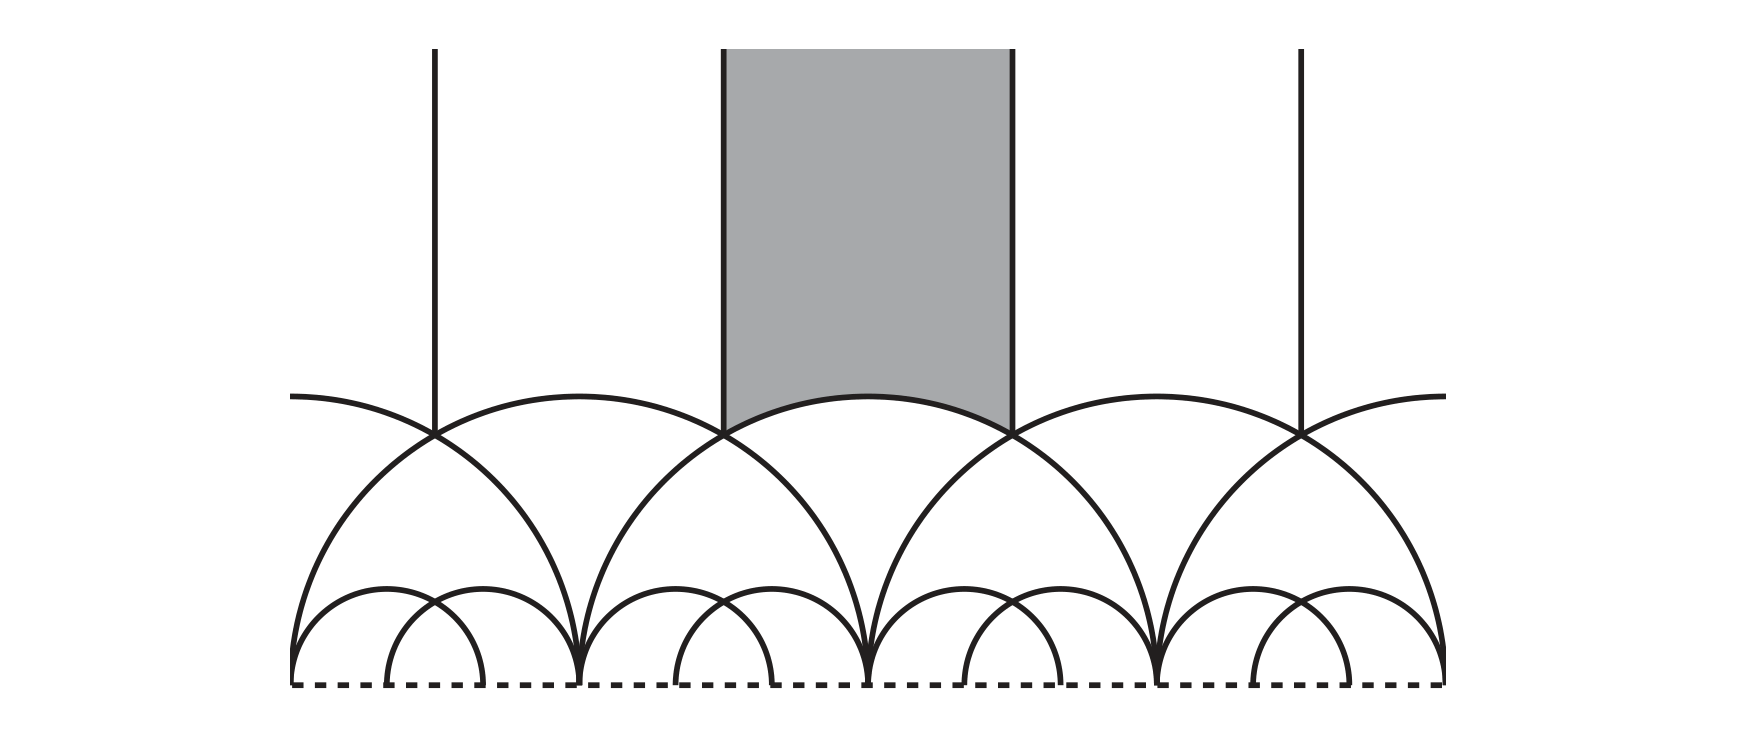
\includegraphics[width=0.52\textwidth]{figure1-1.png}
  \caption{$\mathrm{SL}_2(\Z)$ 作用在 $\mathbb{H}$ 上的基本域（灰色区域）。
    （原文 p.~10，Figure 1.1）}
  \label{fig:1-1}
\end{figure}

\begin{srcex}{1}
若取 $G=\mathrm{Sp}_{2n}(\R)$、$\Gamma=\mathrm{Sp}_{2n}(\Z)$、$K=\mathrm{SO}_n$，
就得到 \emph{Siegel 模形式}。
\end{srcex}

\subsection{结构}

把上述问题看成该局部对称空间上的量子力学，已有很长的历史。但数论中还存在着多得多的结构，
这些结构似乎并不出现在“粒子在该局部对称空间上运动”的量子力学里。

先把情形限制为 $G=\mathrm{SL}_2(\R)$。

\paragraph{数域}
理解
\begin{equation}\tag{1.6}\label{eq:1.6}
L^2\bigl(\mathrm{SL}_2(\Z)\backslash\mathrm{SL}_2(\R)/\mathrm{SO}_2\bigr)
\end{equation}
这一问题，对任意数域都有类比。可以把 $\Z$ 看成有理数域中的整数环：
\begin{equation}\tag{1.7}\label{eq:1.7}
\Z=\mathcal{O}_{\Q}.
\end{equation}
由此得到格 $\mathrm{SL}_2(\mathcal{O}_{\Q})$。这样写出来便可看出：可以把 $\Q$ 换成任意有限扩张 $F$，
于是 $\Z$ 变为整数环 $\mathcal{O}_F$：
\begin{equation}\tag{1.8}\label{eq:1.8}
\begin{aligned}
\Q &\rightsquigarrow F,\\
\Z &\rightsquigarrow \mathcal{O}_F .
\end{aligned}
\end{equation}

% [Tutor Note: 式 (1.8) 只是“换基域”的隐喻性图示，并不是说 $\mathcal{O}_F$ 等于 $\Z$ 作基变换。
%  正确的陈述是：$\mathcal{O}_F$ 是 $F$ 在 $\Q$ 上的整闭包；对 $F/\Q$ 有限，$\Spec\mathcal{O}_F$ 是 $\Spec\Z$ 上的有限平坦覆盖
%  （在分歧素点处退化）。把它读成“base change”会误导后续对分歧的几何理解。]

要点是：当把 $\Q$ 换成另一个数域 $F/\Q$ 时，空间 $\mathcal{M}_{G,\Q}$ 变成某个空间
$\mathcal{M}_{G,F}$。然后取 $L^2$ 或 $H^*$ 将其线性化。

\begin{srcex}{2}
这对所有约化代数群 $G$ 都成立；但取 $G=\mathrm{PSL}_2\R$，则
\begin{equation}\tag{1.9}\label{eq:1.9}
\mathcal{M}_{G,\Q}
  =\mathrm{PSL}_2\Z\backslash\mathrm{PSL}_2\R/\mathrm{SO}_2
\end{equation}
就是图 \ref{fig:1-1} 中的局部对称空间。若把 $\Q$ 换成任意数域 $F/\Q$，就得到
\begin{equation}\tag{1.10}\label{eq:1.10}
\mathcal{M}_{G,F}
  =\mathrm{PSL}_2(\mathcal{O}_F)\backslash
   \mathrm{PSL}_2(F\otimes_{\Q}\R)/K .
\end{equation}
注意
\begin{equation}\tag{1.11}\label{eq:1.11}
F\otimes_{\Q}\R\simeq \R^{\times r_1}\times \C^{\times r_2},
\end{equation}
其中 $r_1$ 是 $F$ 的实嵌入个数，$r_2$ 是复嵌入的共轭对个数。
\end{srcex}

% [Tutor Note: 式 (1.11) 中的记号 $\R^{\times r_1}$ 表示 $r_1$ 个 $\R$ 的直积，$\C^{\times r_2}$ 同理；
%  这里 $\times$ 是“笛卡尔积”而非群乘法。对 $F=\Q(\sqrt{d})$ 可直接验证：实二次域给出两个实嵌入，
%  虚二次域给出一个共轭对。后续计算 $\mathcal{M}_{G,F}$ 的维数/体积时，这个分解是第一道易错关口。]

\begin{srcex}{3}
令 $F=\Q\bigl(\sqrt{d}\bigr)$。若 $F$ 是实的（$d\ge 0$），则 $r_1=2$
（对应 $\pm\sqrt{d}$）、$r_2=0$，于是
\begin{equation}\tag{1.12}\label{eq:1.12}
\mathrm{PSL}_2\Bigl(\Q\bigl(\sqrt{d}\bigr)\otimes_{\Q}\R\Bigr)
  =\mathrm{PSL}_2\R\times\mathrm{PSL}_2\R .
\end{equation}
这引出所谓的 \emph{Hilbert 模形式}。

若 $F$ 是虚的（$d<0$），则 $r_1=0$、$r_2=1$，且
\begin{equation}\tag{1.13}\label{eq:1.13}
\mathrm{PSL}_2\Bigl(\Q\bigl(\sqrt{d}\bigr)\otimes_{\Q}\R\Bigr)
  =\mathrm{PSL}_2\C .
\end{equation}
此时极大紧子群是 $\mathrm{SO}_3\R$，商空间
\begin{equation}\tag{1.14}\label{eq:1.14}
\mathbb{H}^3=\mathrm{PSL}_2\C/\mathrm{SO}_3\R
\end{equation}
是双曲三维空间。接下来要用（左作用的）格作商，得到某个双曲流形，它是图 \ref{fig:1-1}
所示图景的三维版本。
\end{srcex}

\begin{srcrem}{3}
要点在于：变动数域后得到的实群并不那么有趣，只是一些 $\mathrm{PSL}_2$ 的拷贝；
但用来作商的格更强烈地依赖于数域，这才是有意思的部分。
\end{srcrem}

\paragraph{导子/分歧数据}
固定数域 $F=\Q$，可以变动“导子”或“分歧数据”。想法如下：局部对称空间 $\Gamma\backslash\mathbb{H}$
有一族覆盖空间 $\Gamma'\backslash\mathbb{H}$，其中 $\Gamma'$ 是 $\mathrm{SL}_2(\Z)$ 的某个同余子群。
于是可以把 $\Gamma$ 替换为 $\Gamma'$。

这里不一般地定义同余子群，但基本上有两类。对 $N\in\Z$，固定子群
\begin{equation}\tag{1.15}\label{eq:1.15}
\Gamma(N)=\left\{\begin{pmatrix}a&b\\ c&d\end{pmatrix}\equiv \mathrm{id}\pmod N\right\},
\end{equation}
\begin{equation}\tag{1.16}\label{eq:1.16}
\Gamma_0(N)=\left\{\begin{pmatrix}a&b\\ c&d\end{pmatrix}
  \equiv\begin{pmatrix}*&*\\ 0&*\end{pmatrix}\pmod N\right\}.
\end{equation}
想法是：从导子 $N$ 与格 $\Gamma$ 出发，然后在 $N$ 的因子处修改 $\Gamma$。注意即使在此设定中，
我们仍有 $\Gamma(N)$ 或 $\Gamma_0(N)$ 的选择。实际上这些变体构成的集合具有更多结构；
$p$ 处的局部数据与 $\mathrm{SL}_2(\Q_p)$ 的表示论有关。

\paragraph{Hecke 代数作用}
我们已经看到，Hilbert 空间依赖于群、数域以及某些分歧数据。

这个理论的一个非常重要的方面是：这个（函数）向量空间带有远为丰富的结构。这里存在巨大的
“退化”：Laplacian 的本征空间比人们预想的要大得多（不是一维的）。

这种退化由 \emph{Hecke 算子}理论给出。它说的是：Laplacian $\Delta$ 实际上属于一个巨大的
交换算子族，这些算子全都作用在 Laplacian 的本征空间上。对素数 $p$（$p$ 非分歧，即
$p\nmid N$），有 $p$ 处的 Hecke 算子 $T_p$。于是
\begin{equation}\tag{1.17}\label{eq:1.17}
\bigoplus_{p}\C[T_p]\ \circlearrowright\ L^2(\Gamma\backslash G/K).
\end{equation}
这是某种“量子可积系统”：如此多的算子与 Hamiltonian 交换，说明有许多守恒量。\footnote{%
这个例子在文献中常被当作量子混沌的例子（量子混沌是“可积性”的反面）。
混沌的一面与离散子群 $\Gamma$ 无关。更具体地说，这属于“算术量子混沌”的研究，
而后者更接近于可积系统的研究。}

\begin{figure}[htbp]
  \centering
  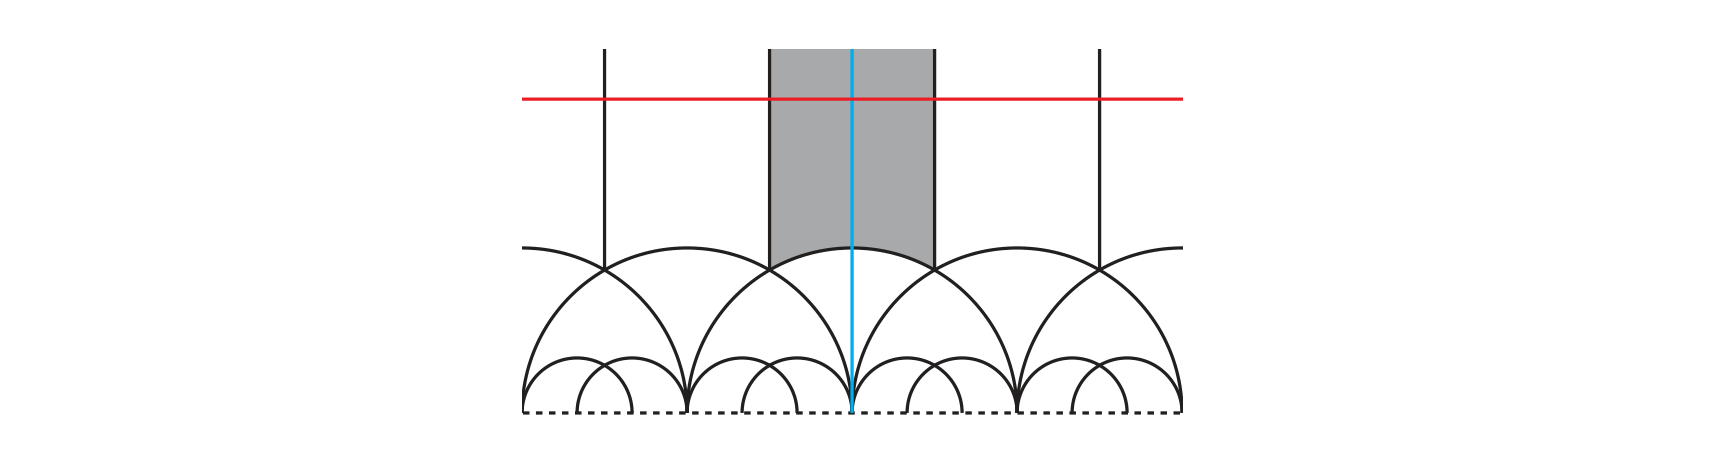
\includegraphics[width=0.52\textwidth]{figure1-2.png}
  \caption{$\mathrm{SL}_2(\Z)$ 作用在 $\mathbb{H}$ 上的基本域（灰色）。
    可以这样定义“周期”：取一个模形式并在例如红线或蓝线上积分。
    （原文 p.~13，Figure 1.2）}
  \label{fig:1-2}
\end{figure}

\paragraph{周期/状态}
有一类特殊的测量可以作用于模形式，称为\emph{周期}（periods）。基本例子是沿直线
$i\R_+\subset\mathbb{H}$ 积分一个模形式，如图 \ref{fig:1-2}。Hecke 正是这样定义 $L$-函数的。

要点是：我们有一族性质非常好的测量/状态，于是可以通过这些周期来研究模形式。

\paragraph{Langlands 函子性}
还有一族略显神秘的算子，其作用对应于变动群 $G$。

\section{Langlands 纲领与 TFT}
\begin{sectionkey}
本节把自守侧的全部结构翻译成四维 TFT 的语言：数域对应三维流形，分歧数据对应余维 $2$
缺陷，Hecke 算子对应线缺陷，周期对应边界条件，函子性对应畴壁；而 $\mathcal{B}$-侧则把
$\pi_1$（或 Galois 群）的表示空间 $\Loc_{G^{\vee}}M$ 上的函数作为输出。由此得到全书主命题
$\mathcal{A}_G\simeq\mathcal{B}_{G^{\vee}}$，它是 Kapustin--Witten 电磁对偶的算术类比。
\end{sectionkey}

\subsection{概览}

我们已经看到，选定约化代数群 $G$ 与数域 $F/\Q$ 后，会得到一个局部对称空间
\begin{equation}\tag{1.18}\label{eq:1.18}
\mathcal{M}=\mathcal{M}_{G,F}
  =\text{“算术格”}\backslash\text{实群}/\text{极大紧子群}.
\end{equation}
它可以被看成 $G$-丛的某个空间
\begin{equation}\tag{1.19}\label{eq:1.19}
\mathcal{M}_{G,F}=\text{“}\Bun_G(\Spec\mathcal{O}_F)\text{”}.
\end{equation}
然后取 $L^2$ 或 $H^*$ 把这个空间线性化。

从自守形式理论出发，在 Hecke 代数作用下作谱分解。Langlands 纲领说：这个分解的各个碎片
对应于 Galois 表示。可以把自守形式理论想象成被送入一个棱镜，从另一侧出来的“颜色”就是
Galois 表示，如图 \ref{fig:1-3}。更具体地说，这些“颜色”是表示
\begin{equation}\tag{1.20}\label{eq:1.20}
\Gal\bigl(\overline{F}/F\bigr)\longrightarrow G^{\vee}_{\C}.
\end{equation}

\begin{figure}[htbp]
  \centering
  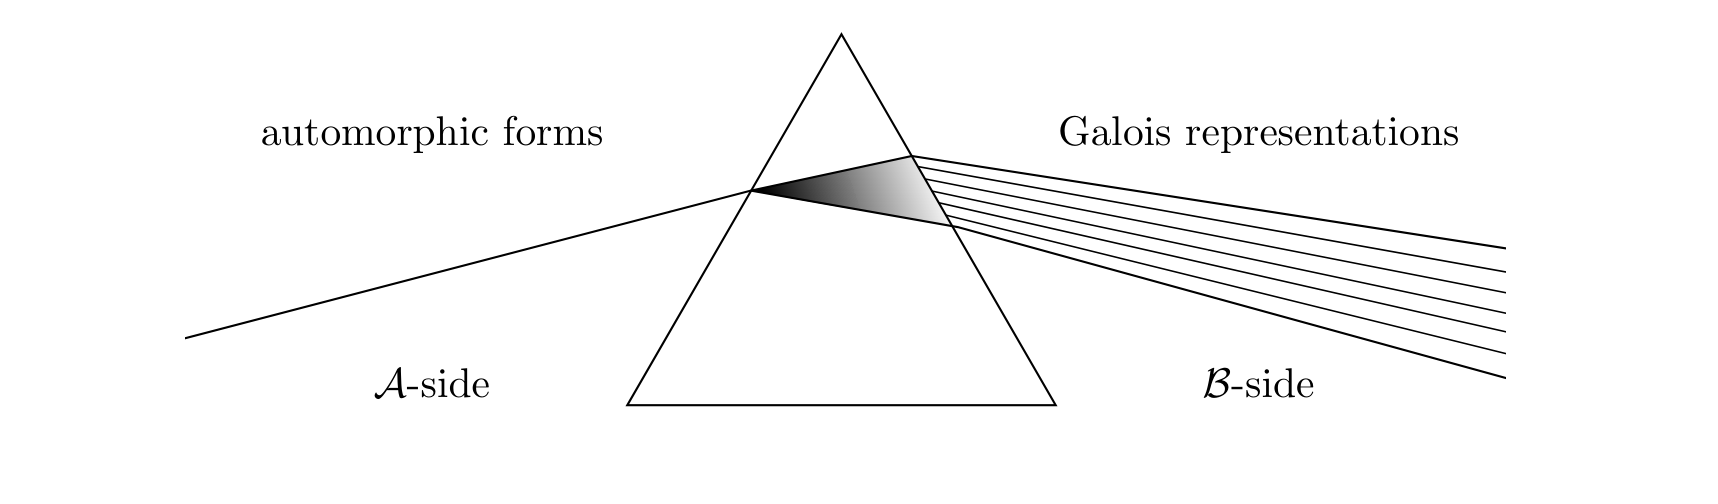
\includegraphics[width=0.55\textwidth]{figure1-3.png}
  \caption{正如光被棱镜分解，这种谱分解把自守形式（$\mathcal{A}$-侧）分解为
    数域的 Galois 表示（$\mathcal{B}$-侧）。（原文 p.~14，Figure 1.3）}
  \label{fig:1-3}
\end{figure}

% [Tutor Note: 式 (1.20) 中的 $G^{\vee}_{\C}$ 指 Langlands 对偶群的 $\C$-点，通常写作 $G^{\vee}(\C)$。
%  这里 $G$ 是 $\Q$ 上的约化群，$G^{\vee}$ 是其复对偶群；而 $\Gal(\overline{F}/F)$ 是绝对 Galois 群。
%  对 $G=\mathrm{GL}_n$，$G^{\vee}=\mathrm{GL}_n(\C)$，这正是通常的 $n$ 维 Galois 表示。对一般 $G$，
%  “$G^{\vee}$-值表示”需要把 Galois 表示与对偶群的中心/连通分量问题一起考虑。]

\begin{srcex}{4}
若 $G=\mathrm{GL}_2\R$，则 $G^{\vee}=\mathrm{GL}_2\C$。设 $E$ 是椭圆曲线，则
\begin{equation}\tag{1.21}\label{eq:1.21}
H^1(E/\Q)
\end{equation}
是 $\Gal(\overline{\Q}/\Q)$ 的二维表示。这正是这个设定中会出现的表示类型。
\end{srcex}

\begin{srcex}{5}
例 4 中的表示非常特殊，只适用于 $\mathrm{GL}_2$。若从 $\mathrm{GL}_3(\R)$ 出发，
相应的局部对称空间 $\mathrm{O}_3\backslash\mathrm{GL}_3\R/\mathrm{GL}_3\Z$
并不是复流形。
\end{srcex}

我们的目标是：把第 \ref{ch:01} 章第 1.1.2 节中的全部结构，与某个物理问题对应起来。
但普通的量子力学太简单了；在物理侧，我们将转而考虑量子场论。

\begin{quote}
\textbf{口号：} Langlands 纲领是四维（算术、拓扑）量子场论研究的一部分。
\end{quote}

具体想法是：Langlands 纲领是四维算术拓扑场论（TFT）之间的等价
\begin{equation}\tag{1.22}\label{eq:1.22}
\begin{array}{ccc}
\mathcal{A}_G & \simeq & \mathcal{B}_{G^{\vee}}\\[2pt]
\text{自守的（automorphic）} & & \text{谱的（spectral）}\\
\text{磁的（magnetic）} & & \text{电的（electric）}
\end{array}
\end{equation}
这两个理论分别称为 $\mathcal{A}$-侧与 $\mathcal{B}$-侧理论。

\begin{srcrem}{4}
这可以称为“四维镜像对称”。这里的 $\mathcal{A}$ 与 $\mathcal{B}$，与通常镜像对称中的
$\mathcal{A}/\mathcal{B}$ 是同一意义。
\end{srcrem}

% [Tutor Note: 式 (1.22) 的物理来源是 Kapustin–Witten 对 4d N=4 超对称 Yang–Mills 的
%  S-对偶作拓扑扭转；A-侧对应自守/磁侧，B-侧对应谱/电侧。它不是已证明的定理，
%  而是组织猜想的原则。这里作者用“等价”一词，读者应理解为“conjectural equivalence
%  of TFTs”；严格陈述需要指明边界条件、算子与范畴的层级。]

一个 $n$ 维 TFT 是这样一种对象：它对每个 $(n-1)$ 维流形指定一个量子力学问题
（或一个向量空间、链复形等）。所以四维 TFT 把三维流形送到某类向量空间。它对低维流形
指定更复杂的数据，对高维流形指定更简单的数据，如表 \ref{tab:1-1} 所示。

\begin{table}[htbp]
  \centering
  \caption{四维拓扑场论的输出。数是最容易理解的，但通常也最难产生（往往需要分析）。
    向量空间也相当简单，但三维流形很难；所以“最佳位置”大约在二维，因为曲面容易理解，
    而范畴也不算太复杂。（原文 p.~15，Table 1.1）}
  \label{tab:1-1}
  \begin{tabular}{c|l}
    \toprule
    Dimension & Output\\
    \midrule
    $4$ & $z\in\C$（很少能在代数上良定义，需要分析）\\
    $3$ & （微分分次）向量空间\\
    $2$ & （微分分次）范畴\\
    $1$ & $(\infty,2)$-范畴\\
    $0$ & $(\infty,3)$-范畴？（很少被理解）\\
    \bottomrule
  \end{tabular}
\end{table}

“拓扑”的意思是：我们扔掉动力学，只看基态。这类似于只看调和形式，而不是 Laplacian 的整个谱。
“算术”的意思是：我们遵循算术拓扑的范式。最终要在数域与三维流形之间建立类比；于是可以把
数域代入 TFT（代替真正的流形），得到一个向量空间，结果正是 $L^2(\mathcal{M}_{G,F})$
（或 $H^*(\mathcal{M}_{G,F})$）。

\subsection{算术拓扑}

\paragraph{Weil 的罗塞塔石碑}
在写给 Simone Weil 的一封信 \cite{Kri05} 中，André Weil 解释了一个漂亮的类比，
现在称为 \emph{Weil 罗塞塔石碑}。它在数域、函数域与 Riemann 面之间建立了三方类比。

一般想法如下。$\Spec\Z$ 是曲线的某种版本，其上的点 $\Spec\F_p$ 对应不同的素数。
$\Spec\Z_p$ 是点周围圆盘的版本，而 $\Spec\Q_p$ 是该点周围去心圆盘的版本。
这类似于代数曲线的通常图景。
\begin{center}
\begin{tabular}{lll}
  \toprule
  曲线 & $\Spec\F_q[t]$ & $\Spec\Z$\\
  点 & $\Spec\F_p$ & $\Spec\F_p$\\
  圆盘 & $\Spec\F_q[[t]]$ & $\Spec\Z_p$\\
  去心圆盘 & $\Spec\F_q((t))$ & $\Spec\Q_p$\\
  \bottomrule
\end{tabular}
\end{center}

% [Tutor Note: 原书此表“圆盘”一行印作 $\Spec\F_t[[t]]$（见 p.15），从上下文看应为
%  $\Spec\F_q[[t]]$：$q$ 是基域 $\F_q$ 的基数，$t$ 是形式参数。这属于原稿笔误，译文按数学上正确的
%  $\F_q[[t]]$ 处理；若读者对照原 PDF 会发现此差异，特此说明。]

一般地，设 $F/\Q$ 是数域，则可考虑 $\mathcal{O}_F$，而 $\Spec\mathcal{O}_F$ 的点对应
$\mathcal{O}_F$ 中的素数。数域与函数域之间的类比如下：从有限域上的光滑射影曲线
$C/\F_q$ 出发，$F$ 的类比是有理函数域 $\F_q(C)$，$\mathcal{O}_F$ 的类比是正则函数环
$\F_q[C]$，最后 $\Spec\mathcal{O}_F$ 的点对应 $C$ 的点。

现在可能想把 $C$ 换成 Riemann 面。设 $\Sigma/\C$ 是紧 Riemann 面，则 $\mathcal{O}_F$ 中的素数
（从而 $C$ 的点）对应 $\Sigma$ 的点。$\Sigma$ 上的亚纯有理函数域 $\C(\Sigma)$ 是 $F$ 的类比。
为了得到 $\mathcal{O}_F$ 的类比，必须从 $\Sigma$ 中去掉一些点（在紧曲线上得不到非平凡函数）。
要点是：数域带有一些“无穷远点”，所以其类比并不是紧 Riemann 面，而是带若干标记点的曲面。
于是 $\mathcal{O}_F$ 的类比由 $\Sigma$ 上在这些点之外正则的函数组成。

这总结在表 \ref{tab:1-2} 中。

\begin{table}[htbp]
  \centering
  \caption{Weil 罗塞塔石碑最初的形态；它在这三列之间建立类比。我们最终会细化这本字典。
    设 $F/\Q$ 是数域，$C/\F_q$ 是有限域上的光滑射影曲线，$\Sigma/\C$ 是紧 Riemann 面。
    $\F_q(C)$ 表示有理函数域，$\F_q[C]$ 表示正则函数环，$\C(\Sigma)$ 表示 $\Sigma$ 上的
    亚纯有理函数。（原文 p.~16，Table 1.2）}
  \label{tab:1-2}
  \begin{tabular}{lll}
    \toprule
    数域 & 函数域 & Riemann 面\\
    \midrule
    $F/\Q$ & $\F_q(C)$ & $\C(\Sigma)$\\
    $\mathcal{O}_F$ & $\F_q[C]$ & 在 $\Sigma$ 的标记点之外正则的函数\\
    $\Spec\mathcal{O}_F$ & $C$ 的点 & $x\in\Sigma$\\
    \bottomrule
  \end{tabular}
\end{table}

\paragraph{缺失的拼块}
现在采取这样的观点：这块罗塞塔石碑缺了一块，我们本应考虑三维流形而不是 Riemann 面。
想法是：$\Sigma/\C$ 真正对应的是 $C/\F_q$。这体现在如下方式中。为了研究点，我们研究映射：
\begin{equation}\tag{1.23}\label{eq:1.23}
\Spec\F_q\hookrightarrow C.
\end{equation}
但从平展拓扑的观点看，$\Spec\F_q$ 并不是真正的点，它更像一个圆，因为
\begin{equation}\tag{1.24}\label{eq:1.24}
\Gal\bigl(\overline{\F}_q/\F_q\bigr)
  =\widehat{\Z}=\pi_1^{\text{étale}}\bigl(\Spec\F_q\bigr),
\end{equation}
其中 $\widehat{\Z}$ 表示 profinite 完备化。因此最好把它想象成一个被修改过的圆，
其中 $\widehat{\Z}$ 由 Frobenius 生成。总有映射
\begin{equation}\tag{1.25}\label{eq:1.25}
\Spec\overline{\F}_q\longrightarrow\Spec\F_q,
\end{equation}
于是可以把曲线提升到 $\overline{\F}_q$。这对应于把这些圆“展开”，即替换为它们的万有覆盖。
于是出现一个 $\R$ 因子，它不参与拓扑/上同调。

于是我们意识到：$\F_q$ 上的曲线具有过多的内部结构，无法与 Riemann 面匹配。

\begin{srcrem}{5}
映射 $\Spec\F_{q^n}\to\Spec\F_q$ 类似于圆的通常 $n$ 重覆盖。
\end{srcrem}

为了修补罗塞塔石碑，我们把 Riemann 面 $\Sigma$ 替换为 $S^1$ 上的某个 $\Sigma$-丛。
具体地说，若给定 $\Sigma$ 与微分同胚 $\varphi$，可以构造映射环面
\begin{equation}\tag{1.26}\label{eq:1.26}
\Sigma\times I\big/\bigl((x,0)\sim(\varphi(x),1)\bigr).
\end{equation}
想法是：若从有限域上的曲线出发，微分同胚 $\varphi$ 就像 Frobenius。

类似地，$\Spec\mathcal{O}_F$ 看起来像一条曲线，其中每个“点”都携带一个圆。所以这同样是
某种三维流形。

\begin{srcrem}{6}
这些圆彼此之间并不“交谈”，因为它们都与不同素数处的 Frobenius 有关。所以它们不太像
乘积或纤维化，而更像带有叶状结构的三维流形。
\end{srcrem}

这与已有的算术拓扑理论相符，该理论有时被称为“纽结与素数”的类比。它始于 Mumford 写给
Mazur 的一封信，但可以归功于许多人，例如 Mazur \cite{Maz73}、Manin、Morishita \cite{Mor10}、
Kapranov \cite{Kap95} 与 Reznikov。Minhyong Kim 的近期工作 \cite{Kim15,CKK19} 起着核心作用。

\begin{srcrem}{7}
这本字典的许多方面已被明确写出，但不应过于直接地使用它。更确切地说，我们应把它理解为：
存在好几类“三维流形”——通常的三维流形、有限域上的函数域，以及数域。
\end{srcrem}

\begin{flushright}
\small 第 2 讲；2021 年 1 月 21 日
\end{flushright}

\paragraph{升级版的罗塞塔石碑}
要点是：我们把罗塞塔石碑中的三个对象都看成三维流形。特别地，把 $\Spec\mathcal{O}_F$
（例如 $\Spec\Z$）看成一个三维流形；于是对任意素数 $p$，有环路
$\Spec\F_p\to\Spec\mathcal{O}_F$，可以把它解释为该三维流形中的一个纽结。
设 $F_v$ 是 $F$ 在素点 $v$ 处的完备化（例如 $\Q_p$），则 $\Spec F_v$ 竟然是该纽结的
管状邻域的边界。要点是：若 $F_v$ 是非 Archimedes 局部域（例如 $\Q_p$ 或 $\F_p((t))$），
其“基本群”就是 Galois 群，并且有商
\begin{equation}\tag{1.27}\label{eq:1.27}
\Gal\bigl(\overline{F}_v/F_v\bigr)\twoheadrightarrow\Z_{\ell}\rtimes\widehat{\Z}.
\end{equation}
这个群称为 \emph{Baumslag--Solitar 群}。具体地，
\begin{equation}\tag{1.28}\label{eq:1.28}
\mathrm{BS}(1,p)=\bigl\{\sigma,u\ \bigm|\ \sigma u\sigma^{-1}=u^{p}\bigr\},
\end{equation}
其中把 $\sigma$ 看作 Frobenius，对应 $\widehat{\Z}$；$u$ 是 $\Z_{\ell}$ 的生成元。其核为
\begin{equation}\tag{1.29}\label{eq:1.29}
p\text{-群}\times\prod_{\ell'\neq\ell,p}\Z_{\ell'}
  \hookrightarrow \Gal\bigl(\overline{F}_v/F_v\bigr)
  \twoheadrightarrow\Z_{\ell}\rtimes\widehat{\Z}.
\end{equation}

% [Tutor Note: 式 (1.27)–(1.29) 描述的是局部域绝对 Galois 群的驯分歧商：
%  惯性群 $I_v$ 的驯部分同构于 $\prod_{\ell'\neq p}\Z_{\ell'}(1)$，而野惯性群是 pro-$p$ 群；
%  商 $\Z_{\ell}\rtimes\widehat{\Z}$ 中的 $\Z_{\ell}$ 来自 $\ell$-进循环（$\ell\neq p$），$\widehat{\Z}$ 由 Frobenius 生成。
%  原文在 (1.29) 前有一句残句 “This tells us that there is For p=1, ...”，
%  其中 “there is” 之后的文字被截断/错位；“p=1” 与 “p=-1” 也不是素数，
%  而是 Baumslag–Solitar 群的退化参数。译文按 BS(1,1)=Z²、BS(1,-1)=Klein 瓶的基本群处理，
%  并保留原文的表述方式。]

这说明：当 $p=1$ 时，这个群是 $\Z\times\Z=\pi_1(T^2)$；当 $p=-1$ 时，它是 Klein 瓶的
基本群。这提供了证据：$\Spec F_v$ 的平展基本群看起来像是环面基本群的某种依赖于 $p$ 的版本。
于是可以把 $\Spec F_v$ 看成一个二维流形（纤维化在 $S^1$ 上）。

经过这番讨论，我们可以给出升级版（多维）的罗塞塔石碑。在三维，我们有：
$\Spec\mathcal{O}_F$、$C/\F_q$，以及映射环面 $T_{\varphi}(\Sigma)$。前两者构成
\emph{整体算术}设定。在二维，首先有局部域，分两类：一类是有限扩张 $F_v/\Q_p$，
另一类是 $\F_q((t))$。这两者的 Spec 都是“二维”的，后者是某种去心圆盘 $D^*$。
它们构成\emph{局部算术}设定。代数闭域（正特征）上的曲线 $C/\overline{\F}_q$ 与
Riemann 面（$\C$ 上的射影曲线 $\Sigma$）也都是“二维”的，它们构成\emph{整体几何}设定。
我们唯一会考虑的四维流形是 $M^3\times I$ 或 $M^3\times S^1$ 的形式，其中 $M^3$ 是
算术或几何来源的三维对象。这些讨论总结在表 \ref{tab:1-3} 中。

\begin{table}[htbp]
  \centering
  \caption{各列对应 Weil 罗塞塔石碑的三个侧面，各行对应维数。我们考虑的四维对象
    只是三维对象与 $S^1$ 或 $I$ 的乘积。$M^3$ 是算术或几何来源的三维对象。
    三维对象是数域、函数域以及 Riemann 面的映射环面。$F$ 是数域，$\varphi$ 是 $\Sigma$
    的某个微分同胚，$T_{\varphi}$ 表示相应的映射环面构造。二维对象是局部域与曲线；
    $F_v$ 是 $\Q_p$ 的有限扩张。一维对象是两种版本的圆，零维对象是点。
    （原文 p.~18，Table 1.3；原表以图像保留）}
  \label{tab:1-3}
  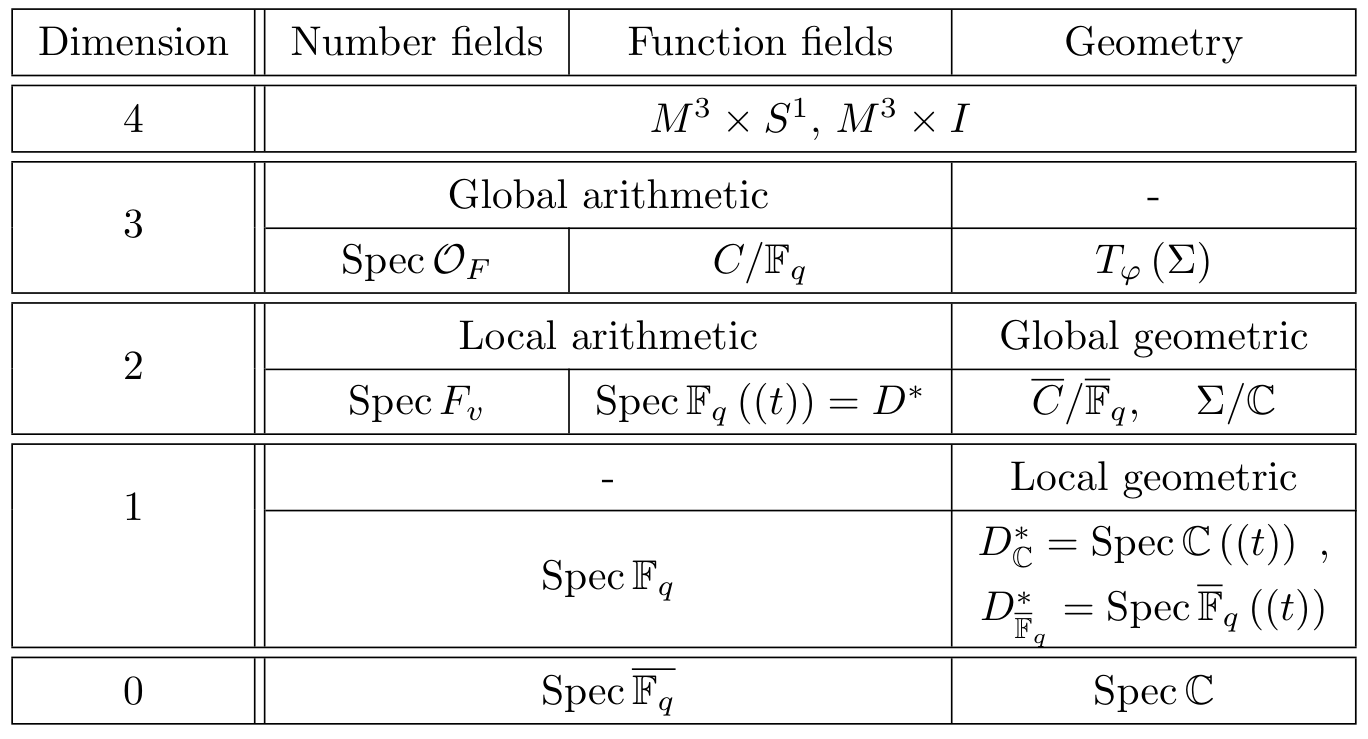
\includegraphics[width=0.82\textwidth]{table1-3.png}
\end{table}

\subsection{$\mathcal{A}$-侧}

$\mathcal{A}$-侧（或自守/磁侧）TFT $\mathcal{A}_G$ 是一台巨大的机器，能做的事很多，
如表 \ref{tab:1-1}。目前唯一能认出的东西是：它把三维流形 $M$ 送到某个向量空间
$\mathcal{A}_G(M)$。我们把 $\Spec\mathcal{O}_F$ 看成三维流形，而对应的赋值正是前面
一直在讨论的向量空间：
\begin{equation}\tag{1.30}\label{eq:1.30}
\mathcal{A}_G(\Spec\mathcal{O}_F)
  =L^2(\mathcal{M}_{G,F})\quad\text{或}\quad H^*(\mathcal{M}_{G,F}).
\end{equation}

\begin{srcrem}{8}
如式 (1.19) 所暗示的，注意 $\Gamma\backslash G/K$ 是所论三维流形上某个东西的模空间，
而不是三维流形本身。
\end{srcrem}

\subsection{结构（重奏）}

事实证明，第 1.1.2 节中自守形式理论的种种“铃铛与哨子”，与 TFT 的种种“铃铛与哨子”
完美地对齐了。

\paragraph{数域}
式 (1.30) 中的赋值形式化了如下想法：我们得到了一个由群与数域标记的向量空间
$L^2(\mathcal{M}_{G,F})$。

\paragraph{导子/分歧数据}
回想分歧数据是一串素数。它体现为三维流形中的一个链环（一族纽结），并允许奇点。
在物理中，它们表现为（余维 $2$ 的）\emph{缺陷}。于是我们先前看到的结构，
体现为该理论的缺陷。

\paragraph{Hecke 代数}
Hecke 算子对应场论中的线缺陷（余维 $3$）。物理上，这相当于沿时空中某个环路
“产生磁单极子”。

\paragraph{周期/状态}
它们对应边界条件，即余维 $1$ 的缺陷。

\paragraph{Langlands 函子性}
从 $G$ 过渡到 $H$，可以解释为穿过畴壁（同样是余维 $1$ 的缺陷）。

\subsection{$\mathcal{B}$-侧}

从数论的观点看，$\mathcal{B}$-侧（或谱侧）是困难的部分，因为数域的 Galois 群
（及其表示）非常难。也就是说，$\mathcal{B}$-侧是问题，而 $\mathcal{A}$-侧是答案。
但从几何的观点看恰好相反，因为 Riemann 面的基本群非常容易。
$\mathcal{B}$-侧研究的是 Galois 表示空间的代数几何。

% [Tutor Note: 原文此处印作 “The B-wide is about studying...”，其中 “B-wide” 显然是
%  “B-side” 的笔误（p.19）。译文按 B-side 处理。]

回想一下：给定三维流形（或数域 $F$），$\mathcal{A}$-侧关心算术局部对称空间
$\mathcal{M}_{G,F}$ 的拓扑。$\mathcal{M}_{G,F}$ 与 $F$ 的几何有关，所以 $\mathcal{A}$-侧
关心 $F$ 的几何的拓扑。

$\mathcal{B}$-侧关心 $F$ 的拓扑的代数。具体如下。对流形 $M$（任意维），可以构造
$\pi_1(M)$。于是 $M$ 上秩 $n$ 局部系统的集合为
\begin{equation}\tag{1.31}\label{eq:1.31}
\Loc_n M=\bigl\{\pi_1(M)\to\mathrm{GL}_n\C\bigr\}.
\end{equation}
局部系统看起来像秩 $n$ 的局部常值层（或带平坦联络的向量丛），有时也称为\emph{特征簇}
（character variety）。然后可以研究 $\C[\Loc_n M]$。

也可以用喜欢的复 Lie 群 $G$ 替换 $\mathrm{GL}_n$，得到
\begin{equation}\tag{1.32}\label{eq:1.32}
\Loc_{G^{\vee}}M=\bigl\{\pi_1(M)\to G^{\vee}\bigr\}.
\end{equation}
它只依赖于 $M$ 的拓扑。

若把数域看成三维流形，则 $\pi_1$ 是 Galois 群的替身，所以这是 Galois 群表示的空间。
TFT 把任意三维流形 $M^3$ 送到 $\Loc_{G^{\vee}}$ 上的函数：
\begin{equation}\tag{1.33}\label{eq:1.33}
\mathcal{B}_{G^{\vee}}\bigl(M^3\bigr)=\C\bigl[\Loc_{G^{\vee}}M\bigr].
\end{equation}

\begin{srcrem}{9}
这一侧写下来比 $\mathcal{A}$-侧容易得多；但若 $M$ 是数域，Galois 群可能非常难以理解。
其余那些“铃铛与哨子”在这里也都容易定义。
\end{srcrem}

\subsection{汇合}

在表 \ref{tab:1-3} 的所有设定中，我们要么作自守测量（附上 $\mathcal{M}_{G,F}$ 并研究其拓扑），
要么取 Galois 群（或 $\pi_1$），由它构造一个簇，再研究其上的代数函数。我们要解释的想法是：
Langlands 纲领是这两个庞大包裹之间的等价，但要对“Langlands 对偶群” $G$ 与 $G^{\vee}$ 而言：
\begin{equation}\tag{1.34}\label{eq:1.34}
\mathcal{A}_G\simeq\mathcal{B}_{G^{\vee}}.
\end{equation}

\begin{srcrem}{10}
在几何设定中已证明的内容比算术设定多，但即便对 Riemann 面的几何 Langlands，
仍是一个未解决的问题。
\end{srcrem}

这实际上是一种把一族猜想组织起来的猜想式方式。

% ============================================================================
% 第 2 章 谱分解（Spectral decomposition）
% 原文 pp. 21--28，Lecture 3（2021-01-26）、Lecture 4（2021-01-28）
% ============================================================================
\chapter{谱分解}\label{ch:02}

\begin{keytakeaways}
本章给出全书反复使用的方法论母题：\term{谱分解}{spectral decomposition}。给定一种“空间”范畴及其上的函数代数 $\cO$，则 $\cO$ 的右伴随 $\Spec$ 把交换代数重新解释为几何对象；反过来，一个模（或表示）就沿 $\Spec\,A$ 铺展成一个层。作者依次列出五部“谱字典”：有限集、紧支撑连续函数（Gelfand--Naimark 定理）、测度空间、代数几何、有理同伦论。第 2.3 节说明经典谱定理的三个版本——矩阵的 Jordan 标准形（代数几何）、von Neumann 投影值测度（可测）、局部常值复形（同伦）——都是同一图景的特例。最后 2.3.4 用“可观测量代数作用于态空间”的物理语言重述这一机制，并指出连续谱中特征向量应被余特征向量（分布）取代：这一区别在后续章节的对偶与反常现象中反复出现。
\end{keytakeaways}

\begin{flushright}\small 第 3 讲；2021 年 1 月 26 日\end{flushright}

\section{什么是谱？}

\begin{sectionkey}
通过函子 $\cO\colon \text{空间}\to\text{交换代数}$ 及其右伴随 $\Spec$ 的伴随关系，把“从代数恢复几何”这一问题形式化；本节列举若干具体“谱字典”，说明 $\Spec$ 在不同范畴中的化身。
\end{sectionkey}

基本想法是：我们从几何的世界出发，也就是我们有一个“空间”的概念（例如代数几何、拓扑……），给定这样一个空间 $X$，我们给它配上某种函数集合 $\cO(X)$。这些函数可以有各种不同的风味，但它们总构成某种交换代数，甚至可能带有更多结构。我们将借助这些函数来把握空间的几何。运算 $\cO$ 其实是一个函子，即若有一个空间之间的态射 $\pi\colon X\to Y$，我们就得到拉回态射 $\pi^{*}\colon \cO(Y)\to \cO(X)$。

关于这一套设置的一个基本问题是：我们能在多大程度上逆转这个操作？于是从任意交换代数出发，我们想理解能在多大程度上从中得到几何。范畴论告诉我们，该考虑的是 $\cO$ 的一个右伴随，我们称之为 $\Spec$。它们构成伴随这一事实意味着：
\begin{equation}\tag{2.1}
\operatorname{Map}_{\mathbf{Spaces}}(X,\Spec\,R)
= \Hom_{\mathbf{Ring}^{op}}\bigl(\cO(X),R\bigr)
= \Hom_{\mathbf{Ring}}\bigl(R,\cO(X)\bigr).
\end{equation}
% [Tutor Note: 这里伴随的方向容易记反。$\cO$ 是反变函子，故其“右伴随”应理解为在 $\mathbf{Ring}^{op}$ 与 $\mathbf{Spaces}^{op}$ 上的左伴随；若忘记取 $op$，就会把 $\Spec$ 误认为左伴随。正确读法是：$\Spec\,R$ 表示“以 $R$ 为函数环的自由空间”，而 (2.1) 表明这种自由性对一切测试空间成立。另注意 $\operatorname{Map}_{\mathbf{Spaces}}$ 必须理解为 plain hom-set（0-截断），否则伴随性只在同伦意义下成立。]

用分析的语言，我们或许可以把 $\Spec\,R$ 看作一个“弱解”，意思是它是“找一个与 $R$ 相伴的空间”这一问题的形式解。它是一个把任意测试空间映为集合的函子，但并不保证真有一个诚实的空间与它相符。

\begin{srcrem}{11}
我们可能必须调整所考虑的范畴，使得
\begin{equation}\tag{2.2}
\cO(\Spec\,R)=R,
\end{equation}
因为这不是伴随性直接给出的。
\end{srcrem}

要点在于，对某一类好的空间，人们可以希望从空间上的函数恢复出空间：$X=\Spec\,\cO(X)$。

\begin{srcrem}{12}
“谱”这个词在数学的许多地方被使用。它们基本上都是一回事，只有同伦论中的谱例外。
\end{srcrem}

\subsection{有限集}

设 $X$ 是有限集，$k$ 是域。则 $k$ 值函数 $\cO(X)$ 可表为
\begin{equation}\tag{2.3}
\cO(X)=\prod_{x\in X}k,
\end{equation}
可以把它想成对角 $X\times X$ 矩阵。

\subsection{紧支撑连续函数}

Gelfand 发展了这一哲学的下述版本。作为我们的空间范畴，考虑局部紧 Hausdorff 空间 $X$ 构成的范畴，态射取连续映射。作为函数空间，我们取 $C_v(X)$，即消失于无穷的连续 $\C$ 值函数空间。这属于交换 $C^{*}$-代数范畴。它们是带有 $*$ 运算（应想成共轭）的 Banach $\C$-代数，该运算 $\C$-反线性且与范数相容。给定任意交换 $C^{*}$-代数 $A$，相伴的谱 $m\text{-}\Spec\,A$ 称为 \term{Gelfand 谱}{Gelfand spectrum}，作为集合它由 $A$ 的极大理想组成。可以把它写成
\begin{equation}\tag{2.4}
m\text{-}\Spec\,A=\Hom_{\C^{*}}(A,\C),
\end{equation}
即 $A$ 的一维酉表示。于是伴随性说的是：
\begin{equation}\tag{2.5}
m\text{-}\Spec\,A=\Hom_{\C^{*}}(A,\C)=\operatorname{Map}(\mathrm{pt},m\text{-}\Spec\,A).
\end{equation}

\begin{srcthm}{1}\textbf{（Gelfand--Naimark）}
$C_v$ 与 $m\text{-}\Spec$ 给出范畴等价。
\end{srcthm}

关于这个定理的更多细节，见例如 [aHRW10]。
% [Tutor Note: 记号 $C_v(X)$ 并非通用记号，通常写作 $C_0(X)$（contract 支撑/消失于无穷）。若 $X$ 非紧，$C_0(X)$ 不含单位元，此时应在单位化代数 $C_0(X)^+$ 上取极大理想，或改用“本原理想/特征”，否则 (2.4) 的 $\Hom_{\C^*}(A,\C)$ 会漏掉零同态之外的信息。作者在正文中默认的应是“含单位的交换 $C^*$-代数”与紧 Hausdorff 空间，非紧情形要靠单位化补救；这是引用 Gelfand--Naimark 时最常见的隐藏约定。]

\subsection{测度空间}

有一个更粗的版本：从测度空间 $X$ 出发，配上（原文 “take attach” 疑为笔误）有界函数 $L^{\infty}(X)$。这构成交换 von Neumann 代数。这同样是范畴等价。

\subsection{代数几何}

我们将聚焦于代数几何的设定。交换代数一侧的范畴就取交换环范畴 $\mathbf{cRing}$。几何一侧取局部环空间范畴。这意思只是说，在每个点上都有“取值”的概念。

函子
\begin{equation}\tag{2.6}
(X,\cO_X)\mapsto \cO(X)
\end{equation}
有伴随
\begin{equation}\tag{2.7}
\Spec\,R \leftarrow R.
\end{equation}
仿射概形构成 $\Spec$ 的像：
\begin{equation}\tag{2.8}
\begin{array}{ccc}
\text{局部环空间} & \longrightarrow & \mathbf{cRing}\\
\uparrow & \qquad\swarrow_{\Spec} &\\
\text{仿射概形} & &
\end{array}
\end{equation}
% 原文内嵌图 p022_d1.png（裁剪含 “nged spaces” 等正文残片，不可直接使用），此处按原版面重排。
% [Tutor Note: (2.8) 的交换图应读成：$\Spec\colon \mathbf{cRing}^{op}\to\mathbf{LocRingSpaces}$ 与“整体截面”函子 $\Gamma$ 的伴随关系在仿射对象上的像；竖箭头表示“仿射概形 $\hookrightarrow$ 局部环空间”的满子范畴包含。作者用图把 $\Spec$ 画成从 $\mathbf{cRing}$ 指向仿射概形，实际方向是反变的，读图时须注意箭头两端是范畴而非函子。]

于是仿射概形与交换环等价这一点本质上是构造中自带的。

这并没有真正捕捉到代数几何中我们想研究的大部分内容，因为人们通常关心一般概形，即局部看起来是仿射的局部环空间。处理这一点的一种办法是真正把几何对象想成：
\begin{equation}\tag{2.9}
\operatorname{Fun}(\mathbf{Ring}^{op},\mathbf{Set})
=\operatorname{Fun}(\mathbf{Aff},\mathbf{Set})
\subset \mathbf{Geometry}.
\end{equation}

\subsection{拓扑}

在同伦论中，我们可能从空间的同伦范畴出发，转向某种函数概念，例如上同调 $H^{*}(X;\Z)$。它位于分次交换环范畴中。这并不直接导致好的谱理论，但若我们记住多一点结构就可以。取而代之，从带连续映射的空间范畴出发，然后取有理链 $C_*^{\Q}$，得到交换微分分次 $\Q$-代数。这就是 Quillen--Sullivan 有理同伦论。\footnote{这一点也应归功于 Mandell。另见 Yuan 的论文 [Yua19]。}事实证明，单连通空间在有理同伦等价下的范畴，等价于在第 0 次为 $\Q$、第 1 次为 $0$ 的交换微分分次代数范畴。

\section{谱分解}

\begin{sectionkey}
对交换环 $R$ 上的模 $V$，利用张量积把 $V$ 沿 $\Spec\,R$ 铺展成拟凝聚层 $\underline{V}$；有限集情形的分解就是按特征子空间分解，而一般情形引出“支撑”与拟凝聚层范畴。
\end{sectionkey}

设 $R$ 是某个域 $k$ 上的交换环。交换环通常通过对它的模的研究而出现。于是设 $V\in R\text{-}\mathbf{mod}$，即有一个映射
\begin{equation}\tag{2.10}
R\to \End(V).
\end{equation}
现在我们想把 $V$ 分解为 $\Spec\,R$ 上的某个层 $\underline{V}$。我们利用 $R\text{-}\mathbf{mod}$ 是对称幺半范畴，故有张量积 $\otimes_R$，于是可对开集 $U\subset\Spec\,R$ 定义
\begin{equation}\tag{2.11}
\underline{V}(U)=V\otimes_R \cO(U).
\end{equation}
然后就可以谈 $v\in V$ 的\term{支撑}{support}：
\begin{equation}\tag{2.12}
\operatorname{Supp}(v)\subset X.
\end{equation}

\begin{srcex}{6}
若 $X$ 有限，即 $R=\prod_{x\in X}k$，则通过要求向量支撑在单点，我们得到分解 $V=\bigoplus_{x\in X}V_x$。但对每个点 $x$，我们都得到一个赋值态射：
\begin{equation}\tag{2.13}
\lambda\colon R\xrightarrow{ev_x}k,
\end{equation}
它与点 $x$ 相伴。和之前一样，可以把它想成一维 $R$-模，因为 $k=\End(k)$。因此改变记号，我们可以把分解写成
\begin{equation}\tag{2.14}
V=\bigoplus_{\lambda\in X}V_\lambda w.
\end{equation}
在这一语言中，分解中的空间正是 $\lambda$-特征空间：
\begin{equation}\tag{2.15}
V_\lambda=\Hom_{R\text{-}\mathbf{mod}}(k_\lambda,V)
=\{v\in V\mid r\cdot v=\lambda(r)v\}.
\end{equation}
\end{srcex}
% [Tutor Note: 印刷版 (2.14) 末尾多出一个 $w$，从上下文看是排版残留（应与 (2.11) 中带下划线的 $\underline{V}$ 记号无关，也不进入任何公式）。照录于此；正确写法应为 $V=\bigoplus_{\lambda\in X}V_\lambda$。另注意 (2.12) 的支撑本应定义为 $\Spec\,R$ 中的闭子集而非 $X$，此处 $X$ 是作者对“底空间”的泛称；在有限集情形二者一致，但一般 $R$ 上应说 $\operatorname{Supp}(v)\subset\Spec\,R$。]

其中 $k_\lambda$ 是 $R$ 上的一维模，$R$ 通过映射 $\lambda$ 作用。

这一描述是通过在一个点处取值给出的，但点既开又闭，所以我们也可把它描述为限制：
\begin{equation}\tag{2.16}
V_\lambda=V\otimes_{\cO(X)=R}k_\lambda,
\end{equation}
因此这个向量空间同时实现为 $\Hom$ 和张量，因为这些点碰巧既开又闭。

定义拟凝聚层范畴为
\begin{equation}\tag{2.17}
\begin{aligned}
\mathrm{QCoh}(X=\Spec\,R) &:= R\text{-}\mathbf{mod}\\
&\ \ \uparrow\\
\mathrm{Coh}(X) &:= R\text{-}\mathbf{mod}_{f.g.}
\end{aligned}
\end{equation}
注意一般 $X$ 只是局部地形如 $\Spec\,R$，所以 $\mathrm{QCoh}(X)$ 只是局部地形如 $R\text{-}\mathbf{mod}$。

\section{谱定理}

\begin{sectionkey}
经典的谱定理（矩阵的 Jordan 形、自伴算子的投影值测度、拓扑空间上局部常值复形）统一为“$A$-模沿 $\Spec\,A$ 层化”的同一机制；2.3.4 给出物理诠释：可观测量代数作用于态空间，测量结果就是层的支撑。
\end{sectionkey}

\subsection{代数几何版本}

设 $V$ 是向量空间，$M\in\End\,V$。可以把 $M$ 想成 $M\in\Hom_{\mathbf{Set}}(\mathrm{pt},\End\,V)$，但 $\End\,V$ 不只是集合。它是 $k$ 上的结合代数，所以实际上
\begin{equation}\tag{2.18}
M\in\Hom_{\mathbf{Set}}(\mathrm{pt},\operatorname{Forget}\End\,V).
\end{equation}
这为与自由 $k$-代数构造的伴随性作好铺垫。一个生成元上的自由代数就是 $k[x]$，于是伴随性说：
\begin{equation}\tag{2.19}
\Hom_{\mathbf{Set}}(\mathrm{pt},\operatorname{Forget}\End\,V)
=\Hom_{k\text{-}\mathbf{Alg}}(k[x],\End\,V).
\end{equation}
我们在这里看到的是：给 $V$ 配上某个 $M\in\End\,V$ 等价于让 $V$ 成为 $k[x]$ 上的模。也就是说，给 $V$ 配上 $M\in\End\,V$ 等价于 $V$ 是 $\Spec\,k[x]=\bA^1$ 上某个拟凝聚层的整体截面。也就是说，$V$ 铺展到 $\bA^1$ 上。

为使之精确，假设 $V$ 有限生成，即层 $\underline{V}$ 凝聚。则 $V$ 有如下作为商与子空间的分解：
\begin{equation}\tag{2.20}
V_{torsion}\hookrightarrow V\twoheadrightarrow V_{tor.\,free},
\end{equation}
其中
\begin{equation}\tag{2.21}
V_{torsion}=\bigcup_{\lambda\in\bA^1}\{v\in V\mid \operatorname{Supp}v=\lambda\}.
\end{equation}
对主理想整环上的普通模（$k[x]$ 是主理想整环）有：
\begin{equation}\tag{2.22}
V\simeq \underbrace{V_{tor}}_{\text{离散谱}}\oplus\underbrace{V_{free}}_{\text{连续谱}},
\end{equation}
其中
\begin{equation}\tag{2.23}
V_{free}=k[x]^{\oplus r}
\end{equation}
以及
\begin{equation}\tag{2.24}
V_{tor}=\bigoplus_{\lambda\in\Spec}V_{\hat\lambda},
\end{equation}
其中 $V_{\hat\lambda}$ 是支撑在 $\lambda$ 处的子空间。事实证明
\begin{equation}\tag{2.25}
V_{\hat\lambda}=\bigoplus_i k[x]/(x-\lambda)^{\ell_i},
\end{equation}
即对这个空间中的任一元素，$(x-\lambda)$ 的某个幂将其零化，所以这些是\term{广义特征空间}{generalized eigenspace}。这个分解恰是 Jordan 标准形。
% [Tutor Note: (2.21) 用并集而非直和，是因为不同 $\lambda$ 上的支撑集合可能相交于 0（即同时在两处支撑的向量只能为 0）；对有限生成模，实际只有有限多个 $\lambda$ 使 $V_{\hat\lambda}\neq 0$，所以该并是有限并、无收敛问题。(2.24) 的下标写成 $\lambda\in\Spec$ 是省略了 $\Spec\,k[x]=\bA^1$；$\hat\lambda$ 表示“以 $\lambda$ 为中心的广义特征空间”，即 (2.25) 中的 $k[x]/(x-\lambda)^{\ell_i}$ 部分，注意它与 (2.16) 的 $V_\lambda$（真特征空间）不同：后者是前者的商。]

特征向量是使 $\lambda v=xv$（或按定义 $Mv$）的某元素 $v\in V$。但这等同于
\begin{equation}\tag{2.26}
\Hom_{k[x]}(k_\lambda,V)
\end{equation}
的一个元素。所以这就是人们可称为“在 $\lambda\in\bA^1$ 处按概形论意义支撑的截面”。

另一方面，纤维
\begin{equation}\tag{2.27}
V\otimes_{k[x]}k_\lambda
\end{equation}
自然地是 $V$ 的商（而非子），所以它们是某种\term{余特征向量}{co eigenvector}。

在连续谱中没有特征向量：作为自由模，$k[x]$ 不含任何特征向量。

\begin{srcex}{7}
考虑自由情形。只需考虑 $V=k[x]$，因为否则它只是它的若干拷贝的直和。此时 $X=\cO_{\bA^1}$。没有广义特征向量（因为对某个 $N\gg0$ 和某个 $\lambda\in\bA^1$，$(x-\lambda)^N=0$）。不过有很多余特征向量。对任意 $\lambda\in\bA^1$，有映射
\begin{equation}\tag{2.28}
V\twoheadrightarrow k_\lambda.
\end{equation}
这是一个分布，即
\begin{equation}\tag{2.29}
\Hom(V,k)
\end{equation}
的一个元素。于是对每个 $\lambda\in\bA^1$，得到
\begin{equation}\tag{2.30}
\Hom(V,k)\ni\delta_\lambda\colon V\twoheadrightarrow k_\lambda.
\end{equation}
\end{srcex}

基本例子是 $V=L^2(\R)$ 和 $M=x$。则 $V_\lambda$ 由支撑在 $x$ 处的函数组成，但一个也没有。我们想说 $\delta_\lambda$，但它不是 $L^2$。对偶算子 $M^{\vee}=d/dx$ 有大致为 $e^{i\lambda x}$ 的特征向量，但它们也不是 $L^2$。

这就是连续谱的样子。当你按 $x$ 或 $d/dx$ 的作用分解 $\bA^1$ 上的函数时，在某种意义上它是\term{直积分}{direct integral}，这与直和不同。你所积分的对象实际上并不是子集。于是我们可以把 $\bA^1$ 上的函数想成“一个点上的函数”的某种连续直和，但这些函数不作为子空间存在。在此情形中它们作为商存在，而非子空间。这在无挠情形更简单，但这是连续谱的一般特征。这并不是分析中的奇怪/特殊事实，因为即使在代数（多项式）层面我们也能看到它。

\subsection{可测版本}

代替矩阵 $M$，我们考虑 Hilbert 空间 $V=\mathcal{H}$ 上的自伴算子 $A$。则 von Neumann 谱定理告诉我们，$\R$ 上有一个“层”（投影值测度）$\pi_A$，且
\begin{equation}\tag{2.31}
A=\int_{\R}x\,d\pi_A.
\end{equation}
投影值测度可按如下方式想成一个层 $\underline{\pi_A}$。对可测集 $U\subset\R$，配上投影下的像：
\begin{equation}\tag{2.32}
\underline{\pi_A}(U)=\pi_A(U).
\end{equation}
所以这是某种 Hilbert 空间层。没有拓扑要与它相容，但它确实满足可加性：规则
\begin{equation}\tag{2.33}
U\mapsto \langle w,\pi_A(U)v\rangle
\end{equation}
定义了 $\R$ 上的 $\C$-值测度。所以这是可测世界中的层版本。
% [Tutor Note: (2.32) 左右两端用同一字母 $\pi_A$ 表示两个不同对象：左边带下划线的是层 $\underline{\pi_A}$，右边是投影算子值测度（对可测集取投影算子）。这种“同一符号、两种范畴”的写法是本节最容易混淆处。另注意 (2.31) 的积分只在 $A$ 自伴时才是实轴上的谱积分；若 $A$ 非自伴（或非正规），应改在 $\C$ 上取谱测度，且 (2.34) 的 $\Spec(A)$ 不再自动是实子集。]

于是式 (2.31) 是说，Hilbert 空间 $\mathcal{H}$ 以某种方式在 $\R$ 上层化，使得 $A$ 通过坐标函数 $x$ 作用，正如上述代数几何设定中那样。于是谱是一个可测子集
\begin{equation}\tag{2.34}
\Spec(A):=\operatorname{Supp}\pi_A\subset\R.
\end{equation}

\begin{srcex}{8}
若 $\mathcal{H}$ 有限维，则谱是离散的点集，分解就是按特征空间分解。
\end{srcex}

\subsection{同伦版本}

我们已看到代数几何中有拟凝聚层、测度论中有投影值测度，现在在代数拓扑中我们有如下。若 $R=C^{*}(X)$，则
\begin{equation}\tag{2.35}
R\text{-}\mathbf{mod}\hookrightarrow \Loc(X),
\end{equation}
其中 $\Loc(X)$ 由 $X$ 上局部常值复形组成。

基本想法是：若我们有 $X$ 上上链的一个模型：
\begin{equation}\tag{2.36}
\to R^{\oplus j}\to R^{\oplus i}\to M,
\end{equation}
则得到 $M$ 由常值层给出的表示：
\begin{equation}\tag{2.37}
\to k_X^{\oplus j}\to k_X^{\oplus i}\to\underline{M},
\end{equation}
其中要点是
\begin{equation}\tag{2.38}
C^{*}(X)=\End^{*}(k_X,k_X).
\end{equation}
或者更直接地，我们可以把层定义为
\begin{equation}\tag{2.39}
\underline{M}(U)=M\otimes_{C^{*}(X)}C^{*}(X).
\end{equation}
% [Tutor Note: 印刷版 (2.39) 右端写作 $C^{*}(X)$，但若如此则右边恒等于 $M$，与开集 $U$ 无关，不可能定义出层。正确形式应是 $\underline{M}(U)=M\otimes_{C^{*}(X)}C^{*}(U)$：用 $U$ 上的上链把常数模 $M$ “局部化”。这里照录原文并加校勘；读者可按修正后的公式理解后面的陈述。(2.35) 的嵌入也不是逐点单射，而是在拟同构意义下把 $R$-模视为 $X$ 上的局部常值复形。]

\begin{flushright}\small 第 4 讲；2021 年 1 月 28 日\end{flushright}

\subsection{物理诠释：可观测量与态}

我们已看到，从某种风味的交换代数 $A$ 出发，可以构造几何对象 $\Spec\,A$。然后 $A$ 上的模 $M$ 铺展成 $\Spec\,A$ 上的层。代数 $A$ 可看成某物理系统的\term{可观测量}{observable}代数。态的集合构成 $A$ 上的模，因而落入这一框架。

让我们退一步。总体想法是，我们试图通过空间上的函数（即进行观测）来把握这个空间的几何。回忆 $\Spec\,A$ 的定义性质：只要有一个空间 $X$ 和映射 $A\to\cO(X)$（其中 $A$ 交换），就得到映射
\begin{equation}\tag{2.40}
X\to\Spec\,A.
\end{equation}
可以把映射 $A\to\cO(X)$ 想成在空间上挑选出满足 $A$ 的关系的一些函数（可观测量）。例如若只有一个函数，这就是从空间到直线的映射，于是空间将在其上分解。一般地，空间会在更高维的底上分解。所以这是用函数测量空间的一种方式。

模的谱分解是这一点的线性化版本。我们把 $X$ 换成它的线性化版本，例如 $\cO(X)$，它就变成 $A$ 上的模。即 $A$ 上的模 $M$ 是映射 $X\to\Spec\,A$ 的线性化版本。若只有一个函数，这对应映射 $X\to\Spec\,k[x]=\bA^1$。同样，单个矩阵（向量空间的自同态）给出 $\bA^1$ 上的一个层。

在量子力学中，我们没有相空间。我们只有一个向量空间 $\mathcal{H}$（相空间的某种线性化版本），称为\term{态 Hilbert 空间}{Hilbert space of states}。可观测量是 $\mathcal{H}$ 上的算子。在物理中我们关心实在性，所以可能坚持可观测量自伴的条件：
\begin{equation}\tag{2.41}
\mathcal{O}=\mathcal{O}^{*}.
\end{equation}
通常我们不会强加这个条件。对可观测量 $\mathcal{O}\circlearrowleft\mathcal{H}$，谱分解告诉我们 $\mathcal{H}$ 在 $\R$ 上层化（作为投影值测度）。底是 $\R$，因为这是单个算子生成的代数的 $\Spec$。这是从经典相空间 $M$ 和单个可观测量 $M\to\R$ 出发、再把 $M$ 在 $\R$ 上分解的类比。

一个\term{态}{state}是元素 $|\varphi\rangle\in\mathcal{H}$。给定一个态和一个算子 $\mathcal{O}$，这个态成为层 $\mathcal{H}$ 的一个截面，即我们得到这个向量的特征空间分解。给定一个截面，我们首先能问的是支撑。这正是我们所做测量“居住”的地方。

利用范数我们可以做得更精确。事实证明，$\|\varphi\|^2$ 是 $\R$ 上的概率测度，告诉我们预期这个态定位在哪里。例如，可取可观测量 $\mathcal{O}$ 在态 $\varphi$ 中的期望值：
\begin{equation}\tag{2.42}
\langle\mathcal{O}\rangle_\varphi
=\frac{\langle\varphi|\mathcal{O}|\varphi\rangle}{\langle\varphi|\varphi\rangle}.
\end{equation}
这是如下式子的连续版本：
\begin{equation}\tag{2.43}
\frac{1}{\langle\varphi|\varphi\rangle}
\sum_{\lambda\in\Spec\,\mathcal{O}}
\lambda\bigl\|\operatorname{Proj}_{\mathcal{H}_\lambda}|\varphi\rangle\bigr\|^2
=
\frac{1}{\langle\varphi|\varphi\rangle}
\sum_{\lambda,\psi_i}
\lambda\langle\psi_i|\varphi\rangle|\psi_i\rangle
\end{equation}
其中 $\psi_i$ 是特征向量的一组基。
% [Tutor Note: 印刷版 (2.43) 右端明显有误：$|\psi_i\rangle$ 是未配对的右矢，且与左端（正数）量纲不符；按 Jordan 谱分解应写成 $\frac{1}{\langle\varphi|\varphi\rangle}\sum_{\lambda,\psi_i}\lambda\,\langle\psi_i|\varphi\rangle\langle\varphi|\psi_i\rangle$，即 $\lambda|\langle\psi_i|\varphi\rangle|^2$。这里照录原文并标出。另注意 (2.42) 的期望值用 $\langle\varphi|\varphi\rangle$ 归一化，与通常“态已归一化”的约定不同；作者在全书中保持这一不归一化的约定，在后续出现 $\langle\mathcal{O}\rangle$ 的地方须与此一致。]

\begin{srcrem}{13}
要给出一个量子力学系统，我们还需要指定\term{哈密顿量}{Hamiltonian} $H$。这是一个特定的可观测量（$\mathcal{H}$ 上的自伴算子），扮演能量泛函的角色。$H$ 的本征态是系统的稳态。这让我们把 $\mathcal{H}$ 铺展到 $\R$ 上，得到能量本征态。我们将在 $H=0$ 的拓扑设定中工作，即我们只看 $0$-特征空间。所以这个分解与我们的关切有些正交。
\end{srcrem}

% ============================================================================
% 第 3 章 Fourier 理论/阿贝尔对偶（Fourier theory/abelian duality）
% 原文 pp. 29--44，Lecture 5（2021-02-02）、Lecture 6（2021-02-04）
% 说明：原文内嵌交换图（p029_d1、p030_d1、p031_d1、p032_d1、p034_d1--d3、
%       p036_d1、p037_d1）的裁剪件均含正文残片或缺标签，故各图按原版面
%       用 LaTeX 数组重排；文件名见各处注释。
% ============================================================================
\chapter{Fourier 理论与阿贝尔对偶}\label{ch:03}

\begin{keytakeaways}
本章把上一章的谱分解机器用于最古典的情形：交换群 $G$ 在其表示上的作用。由于所有算子 $\rho(g)$ 彼此交换，谱由 $G$ 的\term{特征标}{character}（一维酉表示）组成，即对偶群 $G^{\vee}$；Fourier 变换就是“沿 $G^{\vee}$ 层化”的显式版本。作者依次处理：有限群（群代数 $\C G$ 与其交换性）、局部紧 Abel 群（Pontrjagin 对偶，$L^1$ 群代数的 Gelfand 谱）、$\R$ 与环面（经典 Fourier 变换，微分 $\leftrightarrow$ 乘以坐标）、Cartier 对偶（代数群、Hopf 代数与余模、形式完备化）。第 3.7 节把上述对偶统一为 Pontrjagin--Poincaré 对偶 $H^i(M,G)^{\vee}\simeq H^{n-i}(M,G^{\vee})$，并以 A-侧（$\Z$ 系数）/B-侧（$\C^{\times}$ 系数）在 1--4 维的例子（T-对偶、镜像对称、电磁对偶的雏形）作结，汇总于表 3.1。
\end{keytakeaways}

我们已看到，只要有一个“谱字典”，我们就得到谱分解的概念：模变成层，而层的概念取决于具体语境。这给了我们把模代数铺展到空间的几何或拓扑上的一种方式。

为使之有用，我们需要交换代数的有趣来源。交换算子的一种自然来源是有一个 Abel 群 $G$ 作用在向量空间 $V$ 上：给定态射
\begin{equation}\tag{3.1}
\rho\colon G\to\Aut(V),
\end{equation}
我们得到一族算子 $\{\rho(g)\}_{g\in G}$，并可用这些算子对 $V$ 作谱分解。这正是 Fourier 理论的内容。所以我们把 Fourier 理论看成谱分解的某种特例。

\section{特征标}

\begin{sectionkey}
交换群表示的谱由其\term{特征标}{character}（一维表示）构成；所有特征标在逐点乘法下又组成对偶群 $G^{\vee}$。本节建立“表示 $\leftrightarrow$ 对偶群上的层”这一字典的最初版本。
\end{sectionkey}

设 $V$ 是 Abel 群 $G$ 的表示，即有一个映射
\begin{equation}\tag{3.2}
\begin{array}{ccc}
G & \longrightarrow & \Aut(X)\ \subset\ \End(V)\\[2pt]
g & \longmapsto & T_g
\end{array}
\end{equation}
使得 $T_gT_h=T_{gh}$。
% 原文内嵌图 p029_d1.png（裁剪含 “Au” 等正文残片），此处按原版面重排。
% [Tutor Note: 印刷版 (3.2) 写作 $\Aut(X)$，但按上下文（$g\mapsto T_g$ 是 $V$ 上的算子、且右侧为 $\End(V)$）应为 $\Aut(V)$。这是原文笔误，照录并标出。另注意 $\Aut(V)\subset\End(V)$ 只是幺半群包含：$G$ 的群同态经此包含成为到乘法幺半群的映射，这正是下一节 (3.6)--(3.8) 要用“幺半群而非群”作伴随的原因。]

\begin{srcex}{9}
若 $G$ 作用在空间 $X$ 上，而 $V$ 是 $X$ 上的函数，则得到 $G$ 在 $V$ 上的作用。
\end{srcex}

\begin{srcex}{10}
$G$ 总作用在自身之上，因此它作用在 $G$ 自身的函数上。这就是\term{正则表示}{regular representation}。
\end{srcex}

现在我们要作谱分解。首先需要知道谱是什么，所以我们提出如下问题。

\textbf{问题 1.} 可能的特征值是什么？

设 $v\in V$ 是特征向量：
\begin{equation}\tag{3.3}
g\cdot v=\chi(g)v,
\end{equation}
其中
\begin{equation}\tag{3.4}
\chi\colon G\to\Aut_{\C}\,V=\C^{\times}\subset\C
\end{equation}
是群同态，即 $G$ 的一个\term{特征标}{character}。于是可能的特征值是特征标：
\begin{equation}\tag{3.5}
G^{\vee}=\{\text{特征标}\}=\Hom_{\mathbf{Grp}}\bigl(G,\C^{\times}\bigr).
\end{equation}
这就是谱，即我们将在 $G^{\vee}$ 上作谱分解。

\section{有限 Fourier 变换}

\begin{sectionkey}
对有限群 $G$，表示等价于群代数 $\C G$ 上的模；$\Spec(\C G,\ast)=G^{\vee}$ 给出“Fourier 变换 = 沿对偶群层化”的第一个严格版本，并引出对偶群与双对偶同构。
\end{sectionkey}

现在设 $G$ 是有限群。\footnote{这是一个简化假设，这样我们不必担心所考虑的是“哪一类”函数。}我们最终会假设 $G$ 是 Abel 群，但现在还不需要。我们想看到 $G^{\vee}$ 出现在谱处。对复表示 $V$ 有群映射 $G\to\Aut\,V$，但它与包含
\begin{equation}\tag{3.6}
\begin{array}{ccc}
G & \longrightarrow & \Aut\,V\ \subset\ \End(V)\\
& \searrow\llap{\scriptsize 幺半群映射} &
\end{array}
\end{equation}
的复合是一个幺半群映射。换言之，$V$ 给出
\begin{equation}\tag{3.7}
\Hom_{\mathbf{Monoid}}\bigl(G,\operatorname{Forget}(\End\,V)\bigr)
\end{equation}
的一个元素。

和之前一样，我们有伴随性：
\begin{equation}\tag{3.8}
\Hom_{\mathbf{Monoid}}\bigl(G,\operatorname{Forget}(\End\,V)\bigr)
=\Hom_{\C\text{-}\mathbf{Alg}}(?,\End\,V),
\end{equation}
其中缺的项应是某种自由构造。事实证明，答案是\term{群代数}{group algebra}：
\begin{equation}\tag{3.9}
?=\C G.
\end{equation}
这是由标量乘法与 $G$ 的元素之和自由生成的代数。由于群有限，这只是
\begin{equation}\tag{3.10}
\C G=\Bigl\{\sum_{g\in G}f(g)\cdot g\Bigr\},
\end{equation}
其中 $f\colon G\to\C$ 是任意函数。确实我们应把 $f$ 想成测度而非函数。$G$ 有限时没有区别，但对任意 $g\in G$ 我们都想要一个典范元素
\begin{equation}\tag{3.11}
\delta_g=1\cdot g\in\C G,
\end{equation}
意思是系数来自某个在 $g$ 处为 $1$、别处为 $0$ 的 $f$，而这一般不是函数。
% 原文内嵌图 p030_d1.png（裁剪只含 “Aut V/⊂/monoid map” 与箭头），此处按原版面重排。
% [Tutor Note: 当 $G$ 非交换时 $\C G$ 非交换，$\Spec$ 无从谈起；因此本章最终必须限制到 Abel 群（作者随后即如此假设）。(3.10) 把 $\C G$ 写成“函数之和”，实际只在 $G$ 有限时成立；一般 $G$ 应写成有限支撑函数（即测度）的代数，这就是正文紧接着强调“应把 $f$ 想成测度”的原因。]

我们可以把 $\C G$ 想成由元素 $\delta_g$（$g\in G$）生成。代数结构来自卷积：
\begin{equation}\tag{3.12}
\delta_f\ast\delta_g=\delta_{fg}.
\end{equation}
一般地
\begin{align}
f_1\ast f_2&=\sum_g f_1(g)g\ast\sum_h f_2(h)h\tag{3.13}\\
&=\sum_k\Bigl(\sum_{gh=k}f_1(g)f_2(h)\Bigr)k\tag{3.14}\\
&=\sum_k\sum_g f_1(g)f_2(kg^{-1})\cdot k.\tag{3.15}
\end{align}

可用乘法映射 $\mu\colon G\times G\to G$ 表达卷积。有两个投影 $\pi_1$ 与 $\pi_2$：
\begin{equation}\tag{3.16}
\begin{array}{ccc}
G\times G & \xrightarrow{\ \mu\ } & G\\
\swarrow_{\pi_1} & & \searrow^{\pi_2}\\
G & & G
\end{array}
\end{equation}
% 原文内嵌图 p031_d1.png（仅两支对角箭头带 π 标签），此处按原版面重排。

把 $f_1$ 沿 $\pi_1$ 拉回、$f_2$ 沿 $\pi_2$ 拉回，得到 $G\times G$ 上的函数：
\begin{equation}\tag{3.17}
f_1\boxtimes f_2:=\pi_1^{*}f_1\,\pi_2^{*}f_2.
\end{equation}
再沿 $\mu$ 推前，结果就是卷积：
\begin{equation}\tag{3.18}
f_1\ast f_2=\mu_{*}(f_1\boxtimes f_2)=\int_{\mu}f_1\boxtimes f_2.
\end{equation}
要点是：只要有可这样拉回与推前的对象，就能以这种方式定义群代数。

对 $G\circlearrowleft V$，我们把这一切扩充为 $\C G\circlearrowleft V$ 的作用。于是 $G$ 是 Abel 群当且仅当 $(\C G,\ast)$ 是交换代数。所以现在 $G$ 的表示论将在其上作层化的根本对象是
\begin{equation}\tag{3.19}
\Spec(\C G,\ast),
\end{equation}
而事实证明
\begin{equation}\tag{3.20}
\Spec(\C G,\ast)=G^{\vee},
\end{equation}
即
\begin{equation}\tag{3.21}
(\C G,\ast)\simeq\bigl(\cO(G^{\vee}),\cdot\bigr).
\end{equation}

这是 Fourier 变换的第一个版本。想法是：映射 $\Spec\,k\to\Spec\,A$ 等同于态射 $A\to k$，而后者恰是 $G$ 的一维表示，即一个特征标。在此对应下，特征标 $\chi_t\in\C G$（$t\in G^{\vee}$）对应点 $\delta_t\in\cO(G^{\vee})$（$t\in G^{\vee}$）。此外，平移 $g$ 对应乘以 $g^{\vee}$，即特征标
\begin{equation}\tag{3.22}
t\mapsto\chi_t(g).
\end{equation}
% [Tutor Note: (3.21) 的对偶性要成立必须限制在 Abel 群 $G$ 上；$\Spec(\C G,\ast)$ 中的 $\ast$ 提醒读者这里取的是卷积乘法。另注意 (3.22) 的 $g^{\vee}$ 是指 $g$ 在对偶群中对应的特征标 $\chi\mapsto\chi(g)$，而不是某个新变量；下一小节 (3.26) 的双对偶映射会把它讲清楚。]

我们可以稍微改写这一等价，使“这是 Fourier 变换的某种版本”更明显。若 $f$ 是 $G$ 上的函数，则可写
\begin{equation}\tag{3.23}
f=\sum_{t\in G^{\vee}}\hat f(t)\cdot\chi_t.
\end{equation}
这只是用特征标基表示 $f$。然后可把 $\hat f(t)$ 恢复为 $f$ 在这组正交归一的基中的系数。我们还有
\begin{equation}\tag{3.24}
f\ast(-)=\hat f\cdot(-).
\end{equation}

\subsection{隐藏的对称性}

这里有一个隐藏的对称性。$G^{\vee}$ 本身在逐点乘法下是 Abel 群，即
\begin{equation}\tag{3.25}
\chi_{t\cdot s}:=\chi_t\cdot\chi_s.
\end{equation}
把相应的 Abel 群称为 $G$ 的\term{对偶群}{dual group}。

要看出这是一个好的对偶，注意有一个重言映射
\begin{equation}\tag{3.26}
\begin{array}{ccc}
G & \xrightarrow{\ \sim\ } & G^{\vee\vee}\\[2pt]
g & \longmapsto & \{\chi\mapsto\chi(g)\},
\end{array}
\end{equation}
它实际上是同构。

我们可以用更对称的方式建立这一切。有两个投影：
\begin{equation}\tag{3.27}
\begin{array}{ccc}
& G\times G^{\vee} &\\
\swarrow_{\pi_1} & & \searrow^{\pi_2}\\
G & & G^{\vee}
\end{array}
\end{equation}
% 原文内嵌图 p032_d1.png（仅两支对角箭头带 π 标签），此处按原版面重排。
以及一个重言对象，称为\term{万有特征标}{universal character}，生活在 $G\times G^{\vee}$ 上：
\begin{equation}\tag{3.28}
\begin{array}{c}
\chi(-,-)\\[-2pt]
\downarrow\\[-2pt]
G\times G^{\vee}
\end{array},
\end{equation}
即 $G\times G^{\vee}$ 上的函数，由
\begin{equation}\tag{3.29}
\chi(g,t)=\chi_t(g)=\chi_g(t)
\end{equation}
给出。

于是 $f\in\operatorname{Fun}(G)$ 的 Fourier 变换由如下步骤给出：拉到 $G\times G^{\vee}$ 上，乘以 $\chi$，再沿 $\pi_2$ 推前求和：
\begin{equation}\tag{3.30}
f\mapsto\pi_{2*}\bigl(\pi_1^{*}f\cdot\chi\bigr).
\end{equation}
显式地，Fourier 变换是
\begin{equation}\tag{3.31}
\hat f(t)=\sum_g f(g)\overline{\chi(g,t)}
\end{equation}
与
\begin{equation}\tag{3.32}
f(g)=\sum_t\hat f(t)\chi(g,t).
\end{equation}
% [Tutor Note: (3.31) 的复共轭不能丢：在有限 Abel 群上 $\overline{\chi(g,t)}=\chi(g,t)^{-1}$，它正是逆变换中“正交关系”的来源，也是 (3.32) 不含共轭的原因。若把 (3.31)(3.32) 视为互逆变换，还必须补上归一化因子 $1/|G|$（或把 $f$ 视为测度、$\hat f$ 视为函数），作者在这里用的是“测度--函数”约定，故两式表面上不对称。]

我们已同时对角化了所有 $g\in G$ 在 $\operatorname{Fun}(G)$ 上的作用。

对任何带 $G$ 作用的 $V$，我们得到 $(\C G,\ast)$ 在 $V$ 上的作用，于是 $V$ 在 $G^{\vee}$ 上作谱分解，即
\begin{equation}\tag{3.33}
V=\bigoplus_{t\in G^{\vee}}V_{\chi_t},
\end{equation}
其中 $G$ 在子空间 $V_{\chi_t}$ 上按 $\chi_t$ 指定的特征值作用。

这给出有限 Abel 群复表示论的完整图景。同样的形式体系在任何有 Abel 群的设定中都适用。我们将聚焦于拓扑群与代数群的设定。一切看起来大体相同，区别只在于我们考虑哪一类函数。

\section{Pontrjagin 对偶}

\begin{sectionkey}
对局部紧 Abel 群，\term{Pontrjagin 对偶}{Pontrjagin duality}用酉特征标群 $G^{\vee}$ 取代有限群情形下的特征标集合；$L^1$ 群代数的 Gelfand 谱与 Fourier 变换把分析问题翻译为 $G^{\vee}$ 上的函数代数问题。
\end{sectionkey}

设 $G$ 是局部紧 Abel（LCA）群。

\begin{srcex}{11}
$\Z$、$\mathrm{U}(1)$、$\R$、$\Q_p$ 与 $\Q_p^{*}$ 都是（非有限的）例子。
\end{srcex}

定义对偶为\term{酉特征标}{unitary character}之集
\begin{equation}\tag{3.34}
G^{\vee}=\Hom_{\mathbf{TopGrp}}\bigl(G,\mathrm{U}(1)\bigr).
\end{equation}

\begin{srcrem}{14}
不应太惊讶于把 $\C^{\times}$ 换成 $\mathrm{U}(1)\subset\C^{\times}$。若 $G$ 有限，所有特征标理论本来就由 $\mathrm{U}(1)$ 捕获。
\end{srcrem}
% [Tutor Note: 对一般 LCA 群，$G^{\vee}$ 要取紧开拓扑才成为拓扑群（Pontrjagin 定理）；(3.34) 只写了集合。“$G$ 紧 $\Leftrightarrow$ $G^{\vee}$ 离散”这一条（见 p.~35）正是紧开拓扑的直接推论，后文 (3.50)--(3.51) 用它解释 $e^{2\pi inx}\in L^2$ 与 $\delta_n\in\ell^2$ 的差别。]

\subsection{群代数}

谱将再次是群代数的 $\Spec$，但我们需要确定此语境下群代数的恰当定义。

给 $G$ 装备 Haar 测度。之前我们有计数测度，可以在函数与测度之间自由转换（因此特别地它们都既可推前也可拉回）。

现在 $L^1(G)$ 以与式 (3.18) 完全相同的方式具有卷积结构：
\begin{equation}\tag{3.35}
f_1\ast f_2=\int_{g\in G}f_1(h)f_2(gh^{-1})\,dg.
\end{equation}
% [Tutor Note: 印刷版 (3.35) 的被积函数用了自由变量 $h$，而积分变量是 $g$，这在原文中即不一致。按 (3.18) 的推前定义应写成 $\int_{g\in G}f_1(g)f_2(g^{-1}h)\,dg$，或把积分变量改为 $h$。叉积次序（$gh^{-1}$ 还是 $g^{-1}h$）取决于群乘法约定，翻译时照录原文，读者按 $f_1\ast f_2(h)=\int f_1(g)f_2(g^{-1}h)dg$ 校正即可。]

和之前一样，这个卷积来自一个伴随。也就是说，它在 $C^{*}$-代数世界中满足一条泛性质。若有一个表示
\begin{equation}\tag{3.36}
G\to\End(V),
\end{equation}
则它对应一个 $C^{*}$-代数态射
\begin{equation}\tag{3.37}
\bigl(L^1(G),\ast\bigr)\to\End(V).
\end{equation}
% [Tutor Note: 严格说 $L^1(G)$ 只是 Banach $*$-代数而非 $C^*$-代数（$C^*$-包络才得到群 $C^*$-代数 $C^*(G)$）；作者说“$C^*$-代数世界”是口语化的说法。用 $L^1(G)$ 的好处是（对 Abel $G$）Gelfand 理论直接给出 $G^{\vee}$，无需先取包络。]

谱是 Gelfand 谱：
\begin{equation}\tag{3.38}
m\text{-}\Spec\bigl(L^1(G),\ast\bigr)=G^{\vee}.
\end{equation}
这是 Fourier 变换的一个版本，它说：
\begin{equation}\tag{3.39}
\bigl(L^1(G),\ast\bigr)\simeq\bigl(C_v(G^{\vee}),\cdot\bigr),
\end{equation}
其中 $C_v$ 表示消失于无穷的函数。另一个版本说有一个重言映射
\begin{equation}\tag{3.40}
G\to G^{\vee\vee},
\end{equation}
它是同构。

再次地，这可写成对称的形式：
\begin{equation}\tag{3.41}
f\mapsto\pi_{2*}\bigl(\pi_1^{*}f\cdot\chi\bigr),
\end{equation}
其中
\begin{equation}\tag{3.42}
\begin{array}{ccc}
& \chi &\\
& \downarrow &\\
& G\times G^{\vee} &\\
\swarrow_{\pi_1} & & \searrow^{\pi_2}\\
G & & G^{\vee}
\end{array}.
\end{equation}
% 原文内嵌图 p034_d1.png（含 G×G∨ 与两支投影箭头、上方 χ 的标签为正文），此处按原版面重排。

对 $G$ 上任何函数或分布概念，都可作此 Fourier 变换操作。问题是：给定输入的函数类型，另一侧得到什么类型的函数？对 $L^2$ 函数我们简单地得到：
\begin{equation}\tag{3.43}
L^2(G)\xrightarrow{\ \sim\ }L^2(G).
\end{equation}
这些 Fourier 变换概念都有相同的一般特征，其中包括：

（i）群元素平移变成逐点乘法。

（ii）卷积也变成逐点乘法。

（iii）特征标对应点。
% [Tutor Note: (3.43) 右端照印本写作 $L^2(G)$，按 Fourier 变换的定义应为 $L^2(G^{\vee})$（Plancherel 定理：Fourier 变换是 $L^2(G)\to L^2(G^{\vee})$ 的等距同构）。这是原文的记号笔误，特此标出。]

\subsection{Fourier 级数}

取 $G=\mathrm{U}(1)$。则
\begin{equation}\tag{3.44}
G^{\vee}=\Hom_{\mathbf{TopGrp}}\bigl(\mathrm{U}(1),\mathrm{U}(1)\bigr)=\Z,
\end{equation}
其中 $n\in\Z$ 对应
\begin{equation}\tag{3.45}
x\mapsto e^{2\pi inx}.
\end{equation}
于是 Fourier 变换建立等价
\begin{equation}\tag{3.46}
L^2\bigl(\mathrm{U}(1)\bigr)\xrightarrow{\ \sim\ }L^2(\Z)=\ell^2.
\end{equation}
和之前一样，这是对称的。有万有特征标
\begin{equation}\tag{3.47}
\chi\colon (x,n)\mapsto e^{2\pi inx},
\end{equation}
生活在 $\mathrm{U}(1)\times\Z$ 上，并有通常的投影：
\begin{equation}\tag{3.48}
\begin{array}{ccc}
& \mathrm{U}(1)\times\Z &\\
\swarrow & & \searrow\\
\mathrm{U}(1) & & \Z
\end{array}.
\end{equation}
% 原文内嵌图 p034_d2.png、p034_d3.png（分别只含一支投影箭头），此处按原版面重排。

于是可以反着读。特征标
\begin{equation}\tag{3.49}
\Z\to\mathrm{U}(1)
\end{equation}
由 $1\in\Z$ 的像决定，所以 $\Z$ 的特征标由 $\mathrm{U}(1)$ 的点标号。

一般地，在 Pontrjagin 对偶中，$G$ 紧当且仅当 $G^{\vee}$ 离散。具体地，对 $n\in\Z$ 有
\begin{equation}\tag{3.50}
e^{2\pi inx}\in L^2,
\end{equation}
因为 $G$ 紧。类似地，因为 $\Z$ 离散，
\begin{equation}\tag{3.51}
\delta_n\in\ell^2.
\end{equation}

\begin{flushright}\small 第 5 讲；2021 年 2 月 2 日\end{flushright}

\section{Fourier 变换}

\begin{sectionkey}
在 $\R^n$、环面与格上具体化 Pontrjagin 对偶：万有特征标 $e^{2\pi i\langle x,t\rangle}$ 给出经典 Fourier 变换；微分算子 $d/dx$ 对应乘以坐标 $t$，从而把“群论一侧”翻译为“几何一侧”。
\end{sectionkey}

回忆 $\mathrm{U}(1)$ 的 Pontrjagin 对偶是 $\Z$。特征标 $\mathrm{U}(1)\to\mathrm{U}(1)$ 由 $z\mapsto z^{n}$（$n\in\Z$）给出。类似地，$\Z$ 的对偶是 $\mathrm{U}(1)$。

可把 $\mathrm{U}(1)$ 换成环面 $T$，它定义为
\begin{equation}\tag{3.52}
T=\R^{d}/\Lambda=\Lambda\otimes_{\Z}\mathrm{U}(1),
\end{equation}
其中 $\Lambda\subset\Z^{d}$ 是满秩格。$T$ 的对偶是对偶格：
\begin{equation}\tag{3.53}
T^{\vee}=\Lambda^{\vee}.
\end{equation}
类似地，格 $\Lambda$ 的对偶是对偶环面：
\begin{equation}\tag{3.54}
T^{\vee}=\Lambda^{\vee}\otimes_{\Z}\mathrm{U}(1).
\end{equation}
% [Tutor Note: (3.53) 与 (3.54) 的左边都印作 $T^{\vee}$，但二者说的是不同对象的对偶：环面的对偶是格 $\Lambda^{\vee}$（离散），格的对偶是环面 $\Lambda^{\vee}\otimes_{\Z}\mathrm{U}(1)$。作者用同一个符号 $T^{\vee}$ 是记号滥用；后文 (3.81)(3.124) 中的 $T^{\vee}$ 一律指“对偶环面”。这是阅读本节最容易出错处。]

经典 Fourier 变换取 $G$ 为实向量空间。对 $G=\R_x$，对偶是另一个 $\R$：$G^{\vee}=\R_t$。用与之前相同的操作、万有特征标
\begin{equation}\tag{3.55}
\chi(x,t)=e^{2\pi ixt},
\end{equation}
得到通常的 Fourier 变换。对一般实向量空间，对偶是对偶向量空间，特征标是
\begin{equation}\tag{3.56}
\chi(x,t)=e^{2\pi i\langle x,t\rangle},
\end{equation}
其中配对是向量空间与其对偶之间的通常配对。

回忆在 $\mathrm{U}(1)$ 与 $\Z$ 的对偶语境中，特征标对应点。现在情形不同：特征标不再是 $L^2$（因为 $\R$ 不像 $\mathrm{U}(1)$ 那样紧），点也不孤立（因为 $\R$ 不像 $\Z$ 那样离散）。但我们仍有
\begin{equation}\tag{3.57}
f(x)=\int_{\R}\hat f(t)e^{2\pi ixt}\,dt.
\end{equation}

微分 $d/dx$ 的运算对应另一侧的乘以 $t$。我们应把 $d/dx$ 想成群平移的无穷小版本，而平移此前变成乘法。所以这是同一框架的一部分：一侧的群论对应于另一侧的几何。

一般地，设 $G$ 是李群，其 Lie 代数 $\fg$ 交换。有从 $\fg$ 到 $G$ 上向量场的映射
\begin{equation}\tag{3.58}
\fg\to\Vect G\subset\mathrm{Diff}(G),
\end{equation}
并且在
\begin{equation}\tag{3.59}
\operatorname{Forget}\colon \mathbf{Alg}_{\mathrm{Assoc.}}\to\mathbf{Lie}\text{-}\mathbf{Alg}
\end{equation}
与函子
\begin{equation}\tag{3.60}
U\colon \mathbf{Lie}\text{-}\mathbf{Alg}\to\mathbf{Alg}_{\mathrm{Assoc.}}
\end{equation}
之间有伴随，后者把 Lie 代数送到\term{泛包络代数}{universal enveloping algebra}。$\fg$ 交换，所以泛包络代数就是对称代数
\begin{equation}\tag{3.61}
U(\fg)=\operatorname{Sym}^{*}\fg.
\end{equation}
$U\fg$ 现在是作用在 $C^{\infty}(G)$ 上的交换代数。因此可在
\begin{equation}\tag{3.62}
\Spec\,U\fg=\fg^{*}
\end{equation}
上作谱分解/层化。例如对作用在 $\R_x$ 上的 $d/dx$，
\begin{equation}\tag{3.63}
\fg^{*}=\R_t=\Spec_{\R}\R[d/dx=t].
\end{equation}
% [Tutor Note: (3.63) 印刷版右端为 “$\Spec\R\R[d/dx=t]$”，其中连续出现两个 $\R$ 是排版重复，应读作 $\Spec_{\R}\R[d/dx=t]$：即在实系数多项式环 $\R[d/dx]$ 上取 $\Spec$，得到 $\R_t$。这里 $\fg=\R$（$G=\R$ 的交换 Lie 代数），$\fg^{*}=\R_t$ 是“动量/频率”坐标所在的直线，与 (3.57) 中 $t$ 的角色一致。]

\begin{srcex}{12}
$\mathrm{U}(1)$ 的对偶是 $\Z\subset\R_t$。
\end{srcex}

\section{在量子力学中}

\begin{sectionkey}
经典相空间的 $T^{*}M$ 与量子态空间 $L^2(M)$ 给出同一对偶的物理版本：位置算子与动量算子互为 Fourier 对偶；在 $M=\R^n$ 上对角化动量即 Fourier 变换，这就是一维 Abel 对偶（“一维镜像对称”）。
\end{sectionkey}

在我们看到 Fourier 变换如何出现在量子力学中之前，先考虑经典力学。若想建模一个在流形 $M$ 中运动的粒子，则相空间是余切丛 $T^{*}M$，$M$ 上有位置坐标 $q$，纤维方向有动量坐标 $p$。可观测量构成：
\begin{equation}\tag{3.64}
\text{$M$ 上的函数}\otimes\operatorname{Sym}TM.
\end{equation}
在量子力学中，态空间被 $\mathcal{H}=L^2(M)$ 取代。可观测量包含 $\mathrm{Diff}(M)$，即 $M$ 上的微分算子。在其中我们有两块：
\begin{equation}\tag{3.65}
\begin{array}{ccc}
\text{$M$ 上的函数} & \longrightarrow & \mathrm{Diff}(M)\\
TM & \nearrow &
\end{array},
\end{equation}
其中
\begin{equation}\tag{3.66}
p_j=i\frac{d}{dq_j}.
\end{equation}
在经典力学中类似的两块交换。但这里它们差一项才交换：切向量 $\xi\in TM$ 与函数 $f\in\operatorname{Fun}(M)$ 必须满足
\begin{equation}\tag{3.67}
\xi f=f\xi+\hbar f'.
\end{equation}
% [Tutor Note: (3.66) 取 $p_j=i\,d/dq_j$（数学约定，$\hbar$ 已吸收进 $p$），此时 $[p_j,q_k]=i\delta_{jk}$；而 (3.67) 又写成 $\xi f=f\xi+\hbar f'$，两式的归一化并不一致——若按 (3.66)，(3.67) 右端应为 $i f'$（或把 $p$ 改回物理约定 $-i\hbar\partial$）。此外 (3.67) 中 $f'$ 应理解为 $\xi(f)$，即沿 $\xi$ 的方向导数，而非对某个坐标的偏导。这是本节最容易混用的符号。]
% 原文内嵌图 p036_d1.png（仅含两支射入 Diff(M) 的箭头），此处按原版面重排。

总结起来，态看起来像“可观测量的平方根”。位置算子
\begin{equation}\tag{3.68}
q_j\cdot(-)
\end{equation}
被对角化，而动量算子作为导数作用。

我们也可转到\term{动量图景}{momentum picture}，即改为对角化 $p_i$（导数）。对 $M=\R^{n}$，我们有不变向量场的自然基（这是群的好处）。现在可同时对角化
\begin{equation}\tag{3.69}
p_j=i\frac{d}{dx_j}
\end{equation}
以识别
\begin{equation}\tag{3.70}
L^2\bigl(\R^{n}_{q}\bigr)\simeq L^2\bigl(\R^{n}_{p}\bigr),
\end{equation}
这就是 Fourier 变换。人们可以说，这把 $G$ 的量子力学与 Pontrjagin 对偶 $G^{\vee}$ 的量子力学等同起来。这是 Abel 对偶的一维情形，或“一维镜像对称”。

\section{Cartier 对偶}

\begin{sectionkey}
把 Fourier 对偶搬进代数几何：代数群由点函子定义，\term{Cartier 对偶}{Cartier dual} $G^{\vee}=\Hom_{\mathbf{GrpAlg}}(G,\GG_m)$ 在 Hopf 代数层面就是 $\cO(G)^{*}$；有限 Abel 群概形的表示论等价于对偶群上的拟凝聚层。形式完备化（例 19）说明为何需要幂零理想。
\end{sectionkey}

这就是我们一直在做的同一套 Fourier 理论，但处于代数几何语境，即我们考虑代数函数而非连续函数等。我们最终会看到这种对偶出现在物理（电磁对偶）以及数论（类域论）中。

要在代数几何世界中说一个群是什么，需要回顾\term{点函子}{functor of points}的概念。对一个簇 $X$，可联系一个函子 $\mathbf{cRing}\to\mathbf{Set}$，把环 $R$ 送到
\begin{equation}\tag{3.71}
X(R)=\Hom(\Spec\,R,X).
\end{equation}
事实证明，指定这个函子等同于指定 $X$ 本身。

一个簇 $G$ 是\term{代数群}{algebraic group}，若相联系的点函子 $\mathbf{cRing}\to\mathbf{Set}$ 提升为取值于群范畴的函子：
\begin{equation}\tag{3.72}
\begin{array}{ccc}
\mathbf{cRing} & \longrightarrow & \mathbf{Set}\\
& \searrow & \uparrow\\
& \mathbf{Grp} &
\end{array},
\end{equation}
% 原文内嵌图 p037_d1.png（含虚线与竖直箭头），此处按原版面重排。
即
\begin{equation}\tag{3.73}
G(R)=\Hom(\Spec\,R,G)
\end{equation}
是一个群。

\begin{srcrem}{15}
有时在代数群的定义中还假设别的东西，我们这里不假设。
\end{srcrem}
% [Tutor Note: 点函子的 $R$ 取遍所有交换环（不只是域），这是“概形论”代数群与“经典”代数群的关键差别：例如 $\Z$ 作为代数群只在此意义下才是群概形。(3.72) 中的虚线提升不是自动的，它等价于给定 $G(R)$ 的群结构对 $R$ 函子化；作者略去的“群运算与结构态射相容”条件通常还要求乘法、单位、逆都是簇态射。]

\begin{srcex}{13}
考虑 $\bA^1=\GG_a$。作为函子，它送
\begin{equation}\tag{3.74}
R\mapsto (R,+).
\end{equation}
这说的是 $\operatorname{Map}(X,\bA^1)=\cO(X)$。
\end{srcex}

\begin{srcex}{14}
考虑 $\bA^1\setminus 0=\GG_m=\Spec\,k[t,t^{-1}]$。作为函子它送
\begin{equation}\tag{3.75}
R\mapsto (R^{\times},\cdot).
\end{equation}
\end{srcex}

\begin{srcex}{15}
整数构成代数群，其点函子由
\begin{equation}\tag{3.76}
\Z\colon R\mapsto(\Z,+)
\end{equation}
给出。
\end{srcex}

设 $G$ 是 Abel（代数）群。$G$ 的\term{Cartier 对偶}{Cartier dual}是
\begin{equation}\tag{3.77}
G^{\vee}=\Hom_{\mathbf{GrpAlg}}(G,\GG_m),
\end{equation}
其中对偶化对象 $\GG_m$ 来自 $\Aut_k=\GG_m$。

\begin{srcex}{16}
设 $G=\Z/n$。Cartier 对偶是
\begin{equation}\tag{3.78}
\Z/n^{\vee}=\Hom(\Z/n,\GG_m)\simeq\mu_n,
\end{equation}
其中 $\mu_n$ 表示 $n$ 次单位根。作为函子，它送
\begin{equation}\tag{3.79}
R\mapsto \text{$R$ 中的 $n$ 次单位根}.
\end{equation}
\end{srcex}

\begin{srcex}{17}
整数的对偶是 $\Z^{\vee}\simeq\GG_m$，因为 $\Z\to\GG_m$ 由 $1$ 的像决定。类似地，
\begin{equation}\tag{3.80}
\GG_m^{\vee}=\Hom_{\mathbf{TopGrp}}(\GG_m,\GG_m)\simeq\Z=\{z\mapsto z^{n}\}.
\end{equation}
\end{srcex}

\begin{srcex}{18}
更一般地，格 $\Lambda$ 的对偶是对偶环面：
\begin{equation}\tag{3.81}
T^{\vee}=\Lambda^{\vee}\otimes_{\Z}\GG_m,
\end{equation}
所以在 $\C$ 上它大致形如 $(\C^{\times})^{\operatorname{rank}\Lambda}$。类似地，环面 $T$ 与对偶格 $\Lambda^{\vee}$ 互换。
\end{srcex}

为避免技术性，假设 $G$ 有限。\footnote{形式上我们假设 $G$ 是有限 Abel 群概形。}考虑 $G$ 上函数的集合 $\cO(G)$。对偶化并取 $\Spec$ 得到对偶群：
\begin{equation}\tag{3.82}
G^{\vee}=\Spec\,\cO(G)^{*}.
\end{equation}
与其谈群代数，$G$ 上的函数具有群\term{余代数}{coalgebra}的结构如下。$G$ 上的乘法映射诱导 $\cO(G)$ 上的余积：
\begin{equation}\tag{3.83}
\begin{array}{ccc}
G\times G & \xrightarrow{\ \mu\ } & G\\
\cO(G) & \xrightarrow{\ \Delta:=\mu^{*}\ } & \cO(G)\otimes\cO(G)
\end{array}.
\end{equation}
这使 $\cO(G)$ 成为 \term{Hopf 代数}{Hopf algebra}，即 $\cO(G)$ 有乘法与余乘法 $\Delta$。事实上，这是有限维交换且余交换的 Hopf 代数。这些 Hopf 代数的研究结果等价于有限 Abel 群概形的研究。

\begin{srcex}{19}\textbf{（“Fourier 变换”）}
设 $\operatorname{char}k=0$。$\GG_a$ 的 Cartier 对偶是它自身的形式完备化：
\begin{equation}\tag{3.84}
\GG_a^{\vee}=\widehat{\GG}_a,
\end{equation}
其中 $\GG_a$ 的形式完备化由
\begin{equation}\tag{3.85}
\widehat{\GG}_a=\bigcup\Spec\,k[t]/(t^{n})
\end{equation}
给出。$n$ 维向量空间 $V$ 的 Cartier 对偶是对偶的完备化：
\begin{equation}\tag{3.86}
V^{\vee}=\widehat{V^{*}}.
\end{equation}
考虑 $\GG_a=\Spec\,k[x]$，即
\begin{equation}\tag{3.87}
\GG_a=\Spec\,k[x].
\end{equation}
它的特征标应是
\begin{equation}\tag{3.88}
e^{xt}=\sum\frac{(xt)^{n}}{n!},
\end{equation}
但我们需要它是有限和。这在 $t$ 幂零时有意义，即存在 $N\gg0$ 使 $t^{N}=0$。
% [Tutor Note: (3.85) 的并集写成 $\bigcup_n\Spec\,k[t]/(t^n)$ 是（形式）归纳极限而非普通概形：每个 $\Spec\,k[t]/(t^n)$ 是加厚点，其并集是形式概形 $\widehat{\GG}_a$，作为函子它把 $R$ 送到 $R$ 的幂零元集。作者在下一段用“$t$ 幂零/接近 0”来直观解释这一点。另注意 (3.87) 单独作为一条编号公式只是重述 $\GG_a=\Spec\,k[x]$，真正的“特征标公式”是 (3.88)。]
所以当这一点成立，即 $t$ “接近 $0$”时，函数 $e^{\langle x,t\rangle}$ 对 $x\in V$、$t\in V^{*}$ 有定义，并且是 $V$ 的特征标。

类似地，完备化的对偶是 $\GG_a$：
\begin{equation}\tag{3.89}
\GG_a=\widehat{\GG_a}^{\vee}.
\end{equation}
回忆 Fourier 对偶交换
\begin{equation}\tag{3.90}
\bigl(\operatorname{Fun}(G),\ast\bigr)\simeq\bigl(\operatorname{Fun}(G^{\vee}),\cdot\bigr).
\end{equation}
于是 $\Rep(G)$ 在 $G^{\vee}$ 上作谱分解。在代数几何中，表示 $V$ 是 $\cO(G)$ 的\term{余模}{comodule}。即有映射 $G\times V\to V$，取函数得到映射
\begin{equation}\tag{3.91}
V\to\cO(G)\otimes V.
\end{equation}
此外，
\begin{equation}\tag{3.92}
\Rep(G)\simeq\cO(G)\text{-}\mathbf{comod}\simeq\cO(G^{\vee})\text{-}\mathbf{mod}\simeq\QC(G^{\vee}).
\end{equation}
\end{srcex}

\subsection{Fourier 级数例子}

\begin{srcex}{20}
对 $G=\Z$，表示范畴由
\begin{equation}\tag{3.93}
\Rep(\Z)=k[z,z^{-1}]\text{-}\mathbf{mod}
\end{equation}
给出，其中 $z$ 是 $1\in\Z$ 的作用。此作用必须可逆，故包含 $z^{-1}$。于是对偶告诉我们：
\begin{equation}\tag{3.94}
\Rep(\Z)=k[z,z^{-1}]\text{-}\mathbf{mod}=\cO(\GG_m)\text{-}\mathbf{mod}=\QC(\GG_m).
\end{equation}
\end{srcex}

\begin{srcex}{21}
向量空间加一个自同态（矩阵）给出
\begin{equation}\tag{3.95}
\QC\bigl(\bA^1=\Spec\,k[z]\bigr),
\end{equation}
但若是自同构（可逆矩阵）则得到
\begin{equation}\tag{3.96}
\Rep(\Z)\leftrightarrow\QC\bigl(\bA^1\setminus\{0\}\bigr).
\end{equation}
\end{srcex}

\begin{srcex}{22}
在代数几何中
\begin{equation}\tag{3.97}
\Rep(\GG_m)=\text{$\Z$-分次向量空间}=\QC(\Z),
\end{equation}
其中
\begin{equation}\tag{3.98}
V\simeq\bigoplus_{n\in\Z}V_n,
\end{equation}
且 $z\in\GG_m$ 按 $z^{n}$ 作用于 $V_n$。
\end{srcex}
% [Tutor Note: (3.97) 的右边写成 $\QC(\Z)$ 看起来奇怪，但它正是 (3.94) 的对称版本：$\Rep(G)\simeq\QC(G^{\vee})$，取 $G=\GG_m$ 时 $G^{\vee}=\Z$，故 $\Rep(\GG_m)\simeq\QC(\Z)$。注意区分：$\QC(\Z)$ 是 $\Z$（作为离散概形）上的拟凝聚层，即 $\Z$-分次向量空间；而 $\QC(\GG_m)$ 是 $k[z,z^{-1}]$-模。两者在 Fourier 对偶下互换，不要与 (3.94) 的 $\QC(\GG_m)$ 混淆。]

\begin{srcex}{23}\textbf{（拓扑例子）}
下面是一个来自拓扑的 Fourier 级数例子。设 $M^{3}$ 是紧可定向三维流形。\footnote{这将是做电磁学的三维流形。这个 Cartier 对偶将给出电磁对偶。若把数域想成三维流形，则这种对偶落入类域论的框架。}设
\begin{equation}\tag{3.99}
G=\operatorname{Pic}M^{3}
\end{equation}
由 $M^{3}$ 上复线丛（或 $\mathrm{U}(1)$-丛）的同构类组成。这在张量积下构成 Abel 群。可把它想成
\begin{equation}\tag{3.100}
G=\operatorname{Map}\bigl(M^{3},B\mathrm{U}(1)\bigr),
\end{equation}
其中 $B\mathrm{U}(1)$ 表示 $\mathrm{U}(1)$ 的分类空间。同伦意义下可把 $B\mathrm{U}(1)$ 想成
\begin{equation}\tag{3.101}
B\mathrm{U}(1)\simeq\C\PP^{\infty}\simeq K(\Z,2).
\end{equation}
对 $L\in G$，可附上第一 Chern 类
\begin{equation}\tag{3.102}
c_1(L)\in H^{2}(M,\Z),
\end{equation}
它是线丛的完全不变量。所以可取
\begin{equation}\tag{3.103}
G=\Lambda=H^{2}(M,\Z).
\end{equation}
Cartier 对偶是
\begin{equation}\tag{3.104}
G^{\vee}\simeq\Lambda^{\vee}\otimes_{\Z}\GG_m
=\Hom\bigl(H_1(M,\Z),\GG_m\bigr)
=\Hom\bigl(\pi_1(M),\GG_m\bigr),
\end{equation}
其中最后一行来自 $H_1=\pi_1^{\mathrm{ab}}$，而从交换化出发的 $\Hom$ 与从整个群出发的 $\Hom$ 相同。但这正是 $M$ 上的平坦 $\C^{\times}$-丛，即
\begin{equation}\tag{3.105}
G^{\vee}=\Loc_{\C^{\times}}(M).
\end{equation}
这不应太令人惊讶，因为 $G$ 看起来像 $\Z^{n}$，而 Cartier 对偶 $G^{\vee}$ 看起来像 $(\C^{\times})^{n}$。

还可把线丛换成环面丛，即从 $\mathrm{U}(1)$ 过渡到 $\mathrm{U}(1)^{n}\simeq T$。则
\begin{equation}\tag{3.106}
\Bun_T(M)\leftrightarrow\Loc_{T^{\vee}}M,
\end{equation}
其中 $\Loc_{T^{\vee}}M$ 由 $M$ 上平坦 $T^{\vee}$-丛的同构类组成。左边仍像格 $\Lambda$，右边仍像环面 $(\C^{\times})^{n}$。
\end{srcex}

\begin{flushright}\small 第 6 讲；2021 年 2 月 4 日\end{flushright}

\begin{srcex}{24}\textbf{（Fourier 级数）}
取 $\Z$ 为我的 Abel 群 $G$。于是我们有几种对偶概念。一种是
\begin{equation}\tag{3.107}
\Hom_{\mathbf{TopGrp}}\bigl(\Z,\mathrm{U}(1)\bigr)=\mathrm{U}(1),
\end{equation}
另一种是
\begin{equation}\tag{3.108}
\Hom_{\mathbf{TopGrp}}(\Z,\GG_m)=\GG_m,
\end{equation}
即若在 $\C$ 上就是 $\C^{\times}$。

区别在于我们所考虑的函数论。第一种情形有等价
\begin{equation}\tag{3.109}
\ell^2=L^2(\Z)\simeq L^2\bigl(\mathrm{U}(1)\bigr),
\end{equation}
第二种情形有
\begin{equation}\tag{3.110}
\C[\Z]\simeq\cO(\C^{\times}).
\end{equation}
注意
\begin{equation}\tag{3.111}
\cO(\C^{\times})=\C[z,z^{-1}]\subset L^2\bigl(\mathrm{U}(1)\bigr),
\end{equation}
以及
\begin{equation}\tag{3.112}
\C[\Z]\subset\ell^2.
\end{equation}
所以代数版本在某种意义上位于解析故事内部。
\end{srcex}
% [Tutor Note: (3.110) 的 $\C[\Z]$ 是群代数（有限支撑函数），其 Gelfand/代数对偶是 $\cO(\C^{\times})=\C[z,z^{-1}]$；这正是 (3.94) 的另一种写法。(3.111)--(3.112) 说明代数对象（多项式/Laurent 多项式）作为 $L^2$ 的稠密子空间嵌入解析对象，但反之不成立：解析完成包含了代数版本没有的极限点。这一“代数 $\subset$ 解析”的包含关系在第 3.7 节的 A-侧/B-侧对比中会以“有限支撑 vs 局部常值”的形式再次出现。]

\paragraph{题外话 1}
对任何群 $G$，表示论有许多不同版本，可看成来自群代数的不同版本。在对偶一侧，这对应于 $G^{\vee}$ 上的不同结构。

例如，若把群代数取为 von Neumann 代数意义，则得到 $G^{\vee}$ 作为测度空间。若从 $C^{*}$-代数意义的群代数出发，则得到 $G^{\vee}$ 作为（局部紧）拓扑空间。若从离散/代数群代数出发，则得到 $G^{\vee}$ 作为代数簇。
% [Tutor Note: 题外话 1 是全章的方法论总结：同一“对偶群”集合 $G^{\vee}$ 上可装三种不同结构（测度 / 拓扑 / 代数），取决于群代数取哪一类完备化。这不是三种不同的对偶，而是同一对象的三种“几何化身”；第 3.7 节的 A-侧（离散/代数）与 B-侧（紧/解析）之分正是这一点的体现。]

\section{Pontrjagin--Poincaré 对偶}

\begin{sectionkey}
把 Pontrjagin/Fourier 对偶与 Poincaré 对偶结合：$H^{i}(M,G)^{\vee}\simeq H^{n-i}(M,G^{\vee})$。以 A-侧（$\Z$ 系数）与 B-侧（$\C^{\times}$ 系数）在 1--4 维的实例说明 T-对偶、镜像对称与电磁对偶的共同结构（表 3.1）。
\end{sectionkey}

现在我们要给出一系列 Pontrjagin/Fourier 对偶的例子，它们基本上是同一个例子，但会更有趣，因为我们将引入一些拓扑。所有这些对偶陈述的汇总见表 3.1。

设 $M^{n}$ 是紧可定向流形。$M$ 的上同调群将是我们研究对偶理论的 Abel 群。这个对偶说，对 Abel 群 $G$，
\begin{equation}\tag{3.113}
H^{i}(M,G)^{\vee}\simeq H^{n-i}(M,G^{\vee}).
\end{equation}
为使自己相信这建立在正确的基础上，可验证如下配对是非退化的：
\begin{equation}\tag{3.114}
H^{i}(M,G)\otimes H^{n-i}(M,G^{\vee})
\to H^{n}(M,G\otimes G^{\vee})
\to H^{n}\bigl(M,\mathrm{U}(1)\bigr)
\to\mathrm{U}(1),
\end{equation}
其中最后的映射是积分。

下述例子的“维数”最终将对应于相应场论的维数，即我们考虑的几何对象实际上比所列维数低一维，以便得到向量空间。带 $\Z$ 系数的一侧将称为 \term{A-侧}{A-side}，带 $\C^{\times}$ 系数的一侧将称为 \term{B-侧}{B-side}。
% [Tutor Note: (3.113) 的成立需要 $M$ 紧可定向、$G$ 取合适的（有限或紧）系数，并且对偶取 Pontrjagin 对偶（连续特征标）；(3.114) 的第一支用 $G\otimes G^{\vee}\to\mathrm{U}(1)$ 的求值配对，第二支用 $H^{n}(M,\mathrm{U}(1))\cong\mathrm{U}(1)$（紧可定向 $n$ 维流形上的积分），最后一支即积分。若 $M$ 非紧或系数带拓扑，需要改用 Borel--Moore 同调/紧支撑对偶，这是后续章节（电磁对偶的边界条件）会再遇到的细节。]

\subsection{一维}

在此情形我们只是有 A-侧 $\operatorname{Map}(\mathrm{pt},\Z)=\Z$ 与 B-侧 $\operatorname{Map}(\mathrm{pt},\C^{\times})=\C^{\times}$ 互换。可以把它说成：$\Z$ 上的量子力学就是 $\C^{\times}$ 的 QM，意思是这些上面的某类函数空间由 Fourier 理论等同。

\subsection{二维}

二维中的一种对偶是在
\begin{equation}\tag{3.115}
H^{0}(S^{1},\Z)\qquad\text{与}\qquad H^{1}(S^{1},\C^{\times})
\end{equation}
之间，意思是这些上面的函数被等同。注意可把 A-侧写成
\begin{equation}\tag{3.116}
H^{0}(S^{1},\Z)=\pi_0\bigl(\operatorname{Map}(S^{1},\Z)\bigr)=[S^{1},\Z].
\end{equation}
B-侧是
\begin{equation}\tag{3.117}
H^{1}(S^{1},\C^{\times})=\bigl|\Loc_{\C^{\times}}S^{1}\bigr|,
\end{equation}
其中 $\bigl|\Loc_{\C^{\times}}S^{1}\bigr|$ 表示 $\Loc_{\C^{\times}}S^{1}$ 的底层空间，它是一个栈。

A-侧看起来就像 $\Z$，B-侧看起来就像 $\C^{\times}$。这就是我们在做“同一个”例子的意义。

A-侧是到 $\Z$ 的映射的理论，B-侧是某种 $\mathrm{U}(1)$ 规范理论。所谓规范理论，我们只是指在处理局部系统或主丛。

\paragraph{题外话 2（局部系统）}
设 $X$ 是拓扑空间，$G$ 是群（带离散拓扑）。则 $\Loc_G X$ 由 $X$ 上的主 $G$-丛组成。这些是局部同构于常值层 $G$ 的层。也可把它想成
\begin{equation}\tag{3.118}
\Loc_G X=\{\pi_1(X)\to G\},
\end{equation}
其中给定主 $G$-丛，相联系的 $\pi_1$ 表示是\term{单值表示}{monodromy representation}。

若只关心同构类，则这是
\begin{equation}\tag{3.119}
H^{1}(X,G)=\bigl|\Loc_G X\bigr|.
\end{equation}
% [Tutor Note: (3.118) 用的是 $\pi_1(X)\to G$ 的表示/同态集合，但严格说 $\Loc_G X$ 是群胚（每个对象带自同构），(3.119) 才对同构类取 $\pi_0$；$\bigl|\cdot\bigr|$ 就是取 $\pi_0$。(3.117) 中 $S^1$ 的底层空间是栈：$\Loc_{\C^{\times}}S^{1}\simeq \C^{\times}//\Z$（由绕数作用），其“点”比同构类多。]

\subsection{二维}

二维中这种对偶的另一个版本在 A-侧有
\begin{equation}\tag{3.120}
H^{1}(S^{1},\Z),
\end{equation}
在 B-侧有
\begin{equation}\tag{3.121}
H^{0}(S^{1},\C^{\times}),
\end{equation}
即到带离散拓扑的 $\C^{\times}$ 的映射。

在 A-侧：
\begin{equation}\tag{3.122}
H^{1}(S^{1},\Z)=[S^{1},B\Z],
\end{equation}
以及
\begin{equation}\tag{3.123}
B\Z=K(\Z,1)=S^{1}.
\end{equation}
所以 A-侧是到 $S^{1}$ 的映射，B-侧也是到 $\C^{\times}$（$S^{1}$ 的某种版本）的映射。这两个空间由有时称为\term{标量场}{scalar field}的东西组成。

这种对偶理论称为 \term{T-对偶}{T-duality} 或\term{镜像对称}{mirror symmetry}，也称为 $R\leftrightarrow 1/R$ 对偶。
% [Tutor Note: 原文 3.7.2 与 3.7.3 的标题相同（都是 “Two dimensions”），并非重复印刷，而是两个互补的陈述：(3.115) 取 $(H^0,H^1)$，(3.120) 取 $(H^1,H^0)$，即交换 A/B 两侧的同调次数。表 3.1 中两行 “2” 分别对应这两条。T-对偶的半径 $R\leftrightarrow1/R$ 正是这里 $H^1(S^1,\Z)$ 的“格”与 $H^0(S^1,\C^{\times})$ 的“对偶环面”之间的互换在半径上的体现。]

再次，作为群，A-侧就是 $\Z$，B-侧只是 $S^{1}$ 的某种版本。在所有这些例子中有用的一点是把 $\Z$ 换成格 $\Lambda$。对偶结果在
\begin{equation}\tag{3.124}
H^{1}(S^{1},\Lambda)\qquad\text{与}\qquad H^{0}\bigl(S^{1},T^{\vee}_{\C}\bigr)
\end{equation}
之间，其中可把
\begin{equation}\tag{3.125}
H^{1}(S^{1},\Lambda)=[S^{1},T]
\end{equation}
想成，其中 $T$ 是紧格
\begin{equation}\tag{3.126}
\Lambda\otimes_{\Z}S^{1}
\end{equation}
的环面。要点是我们交换到环面的映射与到对偶环面的映射。

\subsection{三维}

设 $\Sigma$ 是紧可定向二维流形。则有对偶
\begin{equation}\tag{3.127}
H^{1}(\Sigma,\Z)\qquad\text{与}\qquad H^{1}(\Sigma,\C^{\times}).
\end{equation}
B-侧是 $\bigl|\Loc_{\C^{\times}}\Sigma\bigr|$，所以 B-侧是三维规范理论（即涉及主丛）。A-侧是
\begin{equation}\tag{3.128}
H^{1}(\Sigma,\Z)=[\Sigma,B\Z=S^{1}],
\end{equation}
所以这是标量场。于是到圆的映射与主丛互换。

\subsection{三维}

另一种方式，在三维中得到对偶
\begin{equation}\tag{3.129}
H^{2}(\Sigma,\Z)\qquad\text{与}\qquad H^{0}(\Sigma,\C^{\times}).
\end{equation}
可把
\begin{equation}\tag{3.130}
H^{2}(\Sigma,\Z)=H^{1}\bigl(\Sigma,\mathrm{U}(1)\bigr)
=[\Sigma,B\mathrm{U}(1)=K(\Z,2)]
\end{equation}
看作由 $\mathrm{U}(1)$-主丛（即线丛）组成，所以这是某种规范理论。另一方面，
\begin{equation}\tag{3.131}
H^{0}(\Sigma,\C^{\times})=[\Sigma,\C^{\times}]
\end{equation}
由标量场组成。所以主丛与到圆的映射互换。再次可升级到环面与格。

\paragraph{题外话 3（向量丛与主丛的字典）}
设 $\mathcal{P}\to X$ 是 $\mathrm{U}(1)$-丛。则可取乘积 $\mathcal{P}\times_{\mathrm{U}(1)}\C$ 构造线丛。一般地若有主 $G$-丛，则有群的一个表示，于是得到向量丛。

反之，若 $\mathcal{L}\to X$ 是线丛，可取它与平凡丛的 $\Hom$：$\Hom(\mathcal{L},X\times\C)$，这是主 $G\mathrm{U}(1)$-丛。
% [Tutor Note: 题外话 3 末尾的 “$G\mathrm{U}(1)$-丛” 是排版错误，应为 “$\mathrm{U}(1)$-丛”：从线丛 $\mathcal{L}$ 出发，$\Hom(\mathcal{L},X\times\C)$ 的纤维是 $\Hom(\C,\C)\cong\C$，但可逆元给出 $\C^{\times}=\mathrm{U}(1)_{\C}$，故得到主 $\C^{\times}$-丛（即 $\mathrm{U}(1)$-丛）。另注意原文把 “principal bundle” 与 “gauge theory” 混用，是课程口语传统，指的都是带联络的主丛。]

\begin{table}[htbp]
  \centering
  \caption{各维数下 Pontrjagin--Poincaré 对偶的例子汇总。（原文 p.~44，Table 3.1）}
  \label{tab:3-1}
  \begin{tabular}{c c c}
    \toprule
    维数 & A-侧 & B-侧\\
    \midrule
    1 & $\operatorname{Map}(\mathrm{pt},\Z)=\Z$ & $\operatorname{Map}(\mathrm{pt},\C^{\times})=\C^{\times}$\\
    2 & $H^{0}(S^{1},\Z)$ & $H^{1}(S^{1},\C^{\times})=\bigl|\Loc_{\C^{\times}}S^{1}\bigr|$\\
    2 & $H^{1}(S^{1},\Z)=[S^{1},S^{1}]$ & $H^{0}(S^{1},\C^{\times})$\\
    3 & $H^{1}(\Sigma,\Z)=[\Sigma,S^{1}]$ & $H^{1}(\Sigma,\C^{\times})=\bigl|\Loc_{\C^{\times}}\Sigma\bigr|$\\
    3 & $H^{2}(\Sigma,\Z)=[\Sigma,B\mathrm{U}(1)]$ & $H^{0}(\Sigma,\C^{\times})$\\
    \bottomrule
  \end{tabular}
\end{table}

\subsection{四维}

四维情形重要，因为两侧都将是规范理论。假设上同调中无挠。对偶在
\begin{equation}\tag{3.132}
H^{2}(M^{3},\Z)\qquad\text{与}\qquad H^{1}(M^{3},\C^{\times})
\end{equation}
之间。

B-侧可写成
\begin{equation}\tag{3.133}
H^{1}(M^{3},\C^{\times})=\bigl|\Loc_{\C^{\times}}M\bigr|,
\end{equation}
即某种规范理论，因为我们在处理 $\C^{\times}$-丛。A-侧是
\begin{equation}\tag{3.134}
[M,K(\Z,2)],
\end{equation}
而同伦型上
\begin{equation}\tag{3.135}
K(\Z,2)=B\mathrm{U}(1)=\C\PP^{\infty}.
\end{equation}
所以 A-侧是
\begin{align}
[M,K(\Z,2)]&=\pi_0\operatorname{Map}(M,\C\PP^{\infty})\tag{3.136}\\
&=\pi_0(\text{$M$ 上的线丛})\tag{3.137}\\
&=\text{线丛}/\sim,\tag{3.138}
\end{align}
即线丛的同构类，所以也是某种规范理论。
% [Tutor Note: 本节标题是“四维”，但 (3.132)--(3.138) 中出现的流形都写作 $M^{3}$：按 3.7 开头声明“几何对象比场论维数低一维”，四维理论的 A-侧应是三维空间 $M^{3}$ 上的线丛/规范场（而 B-侧是 $M$ 上的平坦 $\C^{\times}$-丛）。这里的 $M$ 与 $M^{3}$ 指同一个流形，只是作者在 (3.133) 中省略了上标；[M,K(\Z,2)] 的 $M$ 也应读作 $M^{3}$。这是原文记号不一致处，不影响结论。]

于是等价的向量空间是两侧上的函数。形式陈述是：A-侧上有限支撑函数（或若我们不考虑空间的 $\pi_0$，则局部常值函数）等价于 B-侧上的代数函数。

所有这些对偶陈述的汇总见表 3.1。
% 原文 p.~41 右上角有一 PDF 注释框「transition between lectures」（指向例 24），无数学内容，故不录入正文。

% ============================================================================
%  第 4 章 电磁对偶（原书 pp. 45--60）
%  译自 David Ben-Zvi, "Between Electric-Magnetic Duality and the Langlands Program"
%  Lecture notes by Jackson Van Dyke, UT Austin, Spring 2021.
% ============================================================================
\chapter{电磁对偶}\label{ch:04}

\begin{keytakeaways}
本章把电磁对偶讲成一个可以精确陈述的数学机制。$U(1)$ 规范理论的场空间
$\cC(M)$ 是一个（无穷维）交换 Lie 群，它（非典范地）分裂为格
$\Lambda=H^{2}(M,\Z)$、环面 $T=H^{1}(M,U(1))$ 与向量空间 $V$ 的乘积；把
$F$ 换成 $\star F$ 相当于在这个群上做 Fourier 变换（Pontrjagin 对偶），于是
格（磁通量）与环面（电通量）互换，\emph{'t Hooft} 算子与 Wilson 算子互换。
二维时这退化为 $R\leftrightarrow 1/R$ 的 T-对偶。为了摆脱度量与分析上的困难，
作者随后转入拓扑扭转：把量子力学扩充为 $\mathcal{N}=1,2,4$ 超对称代数，并在
$Q$-上同调中把 Hilbert 空间取成形如 $H^{\bullet}_{U(1)}(\cC(M))$ 的等变上同调。
由此得到 A、B 两类拓扑理论：A-扭转研究 $\mathrm{Pic}(M)$ 的拓扑，B-扭转研究
$\Loc_{\C^{\times}}(M)$ 的代数几何，而电磁对偶恰好交换二者。最后用类时线缺陷与
面缺陷（分歧／螺线管）说明“造磁单极子”与“造电粒子”的对偶。
\end{keytakeaways}

我们此前见过的那些对偶陈述，都只是电磁对偶投下的一个影子。我们将追随
Witten [DEF$^{+}$99]、Freed [Fre00] 以及 Freed--Moore--Segal [FMS07] 的讲法。

\section{经典场论}
\begin{sectionkey}
先在最简单的二维与三维情形里观察对偶的原型：把一个周期标量场 $\varphi$ 的
1-形式 $u=d\varphi$ 换成 $\star u$，方程的形状保持不变，但其几何含义从
“调和映射”变成了“Maxwell 方程”，尺度 $R$ 也变成 $1/R$。
\end{sectionkey}

\subsection{二维}
\label{sec:4-1-1}

我们先研究二维经典场论。设 $\Sigma$ 为黎曼 2-流形。

考虑一个\term{周期标量场}{periodic scalar field}，即一个光滑映射：
\begin{equation}\tag{4.1}
\varphi\in \mathrm{Map}_{C^{\infty}}(\Sigma,S^{1}).
\end{equation}

现在有一个自然的经典场方程要求它满足：\term{调和映射方程}{harmonic map equation}。

方便起见，引入 $\Sigma$ 上的 1-形式 $u=d\varphi$，于是可以写下这组方程：
\begin{equation}\tag{4.2}
\begin{cases}
du=0\\
d\star u=0
\end{cases}.
\end{equation}

第一个方程自动成立，因为 $u$ 已经是恰当形式。第二个方程等价于
$\star d\star u=0$，而这又等价于 $\varphi$ 是调和的。

我们把 (4.2) 写成这种形式，是因为它在 $u\mapsto\star u$ 之下是对称的。换言之，
标量 $\varphi$（满足 $d\varphi=u$）的理论，与某个 $\varphi^{\vee}$（满足
$d\varphi^{\vee}=\star u$）所对应的理论是同一个理论。如果要把度量也纳入考虑，
那么我们研究的是映入某个半径 $R$ 的圆的调和映射，而对偶理论研究的则是映入半径
$1/R$ 的圆的调和映射。这就是 $R\leftrightarrow 1/R$ 对偶。

\begin{srcrem}{16}
对微分形式而言，Poincaré 对偶是由 Hodge 星 $\star$ 实现的，所以我们离之前
所处的地方并不远。
\end{srcrem}

% [Tutor Note: 此处 $\star$ 的归一化约定很关键：$\star\star=\pm1$（黎曼 2-流形上
% 对 1-形式 $\star^{2}=+1$，对 3-维 Lorentz 流形上的 2-形式 $\star^{2}=-1$）。
% 作者在 (4.9) 中取 $B^{\vee}=-\star_{3}E$、在 (4.10) 中取 $E^{\vee}=\star_{3}B$，
% 正是为保证 $(\star F)$ 的分量恰为 $(B^{\vee},E^{\vee})$；若采用相反的 Hodge 星
% 约定，这两个符号会同时反号，$R\leftrightarrow 1/R$ 的结论不变。]

\subsection{三维}
\label{sec:4-1-2}

在三维情形可以玩同样的把戏。设 $\varphi\in \mathrm{Map}_{C^{\infty}}(\Sigma,S^{1})$
为标量场，并令 $u=d\varphi$。我们再次把调和映射方程写成这个漂亮的形式：
\begin{equation}\tag{4.3}
\begin{cases}
du=0\\
d\star u=0
\end{cases}.
\end{equation}

% [Tutor Note: 原文这一段的定义域仍写作 $\Sigma$，但本小节标题与上下文都是三维，
% 因此这里应理解为 3-流形 $M^{3}$；照原样保留记号 $\Sigma$，读者按 $M^{3}$ 理解即可。]

现在从 $u$ 过渡到 $\star u$，是从 1-形式过渡到 2-形式，所以它甚至不再是同一类
对象了。记 $F=\star u$。局部上可以写成
\begin{equation}\tag{4.4}
F=dA
\end{equation}
其中 $A$ 是某个 1-形式，于是我们得到方程
\begin{equation}\tag{4.5}
\begin{cases}
dF=0\\
d\star F=0
\end{cases},
\end{equation}
这正是三维 Maxwell 方程。因此标量场 $\varphi$ 的理论对偶于一个满足 Maxwell
方程的场 $F$ 的理论。

\section{四维／Maxwell 理论入门}
\begin{sectionkey}
在四维 Minkowski 空间中把电场 $E$ 与磁场 $B$ 组装成场强
$F=B-dt\wedge E$，则真空 Maxwell 方程在 $F\leftrightarrow\star F$ 下对称，
这给出 $E\leftrightarrow B$ 的对偶；有源情形下电、磁流的引入会破坏这一对称，
而势 $A$ 的存在（$F=dA$）正是破坏的来源，它导致 Dirac 电荷量子化与
Bohm--Aharonov 效应。
\end{sectionkey}

\term{电场}{electric field}是一个 1-形式 $E\in\Omega^{1}(\R^{3})$，
\term{磁场}{magnetic field}是一个 2-形式 $B\in\Omega^{2}(\R^{3})$。
从相对论的角度看，更好的做法是考虑一个复合的对象，称为\term{场强}{field strength}：
\begin{equation}\tag{4.6}
F=B-dt\wedge E\in\Omega^{2}(M^{4}).
\end{equation}
其中 $M^{4}$ 是 Minkowski 空间。也就是说，我们需要把 $E$ 变成 2-形式，于是用
时间来楔它，这样才能从 $B$ 中把它减掉。

真空中的 Maxwell 方程是：
\begin{equation}\tag{4.7}
\begin{cases}
dF=0\\
d\star F=0
\end{cases}.
\end{equation}
注意它在交换 $F$ 与 $\star F$ 之下是对称的。一些代数运算表明：
\begin{equation}\tag{4.8}
\star F=B^{\vee}-dt\wedge E^{\vee},
\end{equation}
其中 $B^{\vee}$ 是 $E$ 的三维 Hodge 星：
\begin{equation}\tag{4.9}
B^{\vee}=-\star_{3}E,
\end{equation}
类似地
\begin{equation}\tag{4.10}
E^{\vee}=\star_{3}B.
\end{equation}
结论就是：Maxwell 方程在交换 $E$ 与 $B$ 之下是对称的。

如果不在真空中，即存在某些流，那么 Maxwell 方程变成：
\begin{equation}\tag{4.11}
\begin{cases}
dF=j_{B}\\
d\star F=j_{E}
\end{cases}
\end{equation}
其中 $j_{B}$ 是\term{磁流}{magnetic current}，$j_{E}$ 是\term{电流}{electric current}。
它们是 3-形式 $j_{B},j_{E}\in\Omega^{3}(M^{4})$。

这些流的含义在于它们与总电荷有关：
\begin{equation}\tag{4.12}
\int_{M^{3}}j_{B}=Q_{B},
\qquad
\int_{M^{3}}j_{E}=Q_{E},
\end{equation}
这里取 $M^{4}=M^{3}\times\R$。若使用 Stokes 定理，就得到 Gauss 定律。它说：
对闭曲面 $\Sigma\subset M^{3}$，磁通量可以表示为
\begin{equation}\tag{4.13}
b_{\sigma}=\int_{\Sigma}F=\#\,Q_{B,\Sigma}
\end{equation}
其中 $\#$ 是某个标量，$Q_{B,\Sigma}$ 是 $\Sigma$ 内的总磁荷。类似地，电通量为
\begin{equation}\tag{4.14}
e_{\Sigma}=\int_{\Sigma}\star F=\#\,Q_{E,\Sigma}.
\end{equation}

% [Tutor Note: (4.13)、(4.14) 右端的 “$\#$” 是作者留的占位符，原书从未给出它
% 的具体数值。按 Gauss 单位制，$b_{\Sigma}=\int_{\Sigma}F=4\pi Q_{B,\Sigma}$，
% 即在 SI 有理化单位制之外出现 $4\pi$ 因子；这说明这里的 $\#$ 实际是与单位制
% 约定有关的常数（例如 $4\pi$），而不是数学上的未知量。]
% [Tutor Note: (4.13) 左边下标误作 $\sigma$（应随右端作 $\Sigma$），而 (4.19)
% 中积分域写作 $\sigma$、右端又保留未展开的 \texttt{[Sigma]}，这三处是同一处
% 排版疏漏；译文按原样保留 $\sigma$ 并在 (4.19) 处以 $[\Sigma]$ 呈现。]

如果你学过电磁学，大概记得 (4.13) 的右端是 0。这是因为现实中似乎不存在任何
磁单极子，即 $Q_{B}=0$，于是 Gauss 定律说 $\int_{\Sigma}F=0$。正是由于这一性质，
我们可以引入电磁势 $A$，写成：
\begin{equation}\tag{4.15}
F=dA.
\end{equation}
注意这在电与磁之间破坏了对称性，因为 $dF=0$ 现在自动成立。特别地，这意味着
$j_{B}=0$。回忆我们应当考虑
\begin{equation}\tag{4.16}
\nabla=d+A,
\end{equation}
把它看作 $M$ 上某个 $U(1)$-丛上的联络。

场强 $F$ 是有意义的东西，但势 $A$ 带有某种含混性，因为它是 $F$ 的某种原函数。
这种含混性由\term{规范变换}{gauge transformation}
\begin{equation}\tag{4.17}
\nabla\rightsquigarrow g^{-1}\nabla g
\end{equation}
刻画，其中 $g\colon M\to U(1)$。类似地
\begin{equation}\tag{4.18}
A\mapsto A+g^{-1}dg,
\end{equation}
也就是说，$A$ 被平移了某个导数，而这不影响 $F$。

事实上，这是可以被实验测量到的。它称为 \term{Bohm--Aharonov 效应}{Bohm--Aharonov effect}。
即使 $F=0$（平坦联络，即 $E=0$、$B=0$），这个联络的单值性仍是可观测的：
带电粒子沿环路运动时会获得一个相位。

现在可以把这一切设想成任意定向黎曼 4-流形上的联络。当我们从 $F$ 过渡到
$\nabla=d+A$ 时，就实现了 \term{Dirac 电荷量子化}{Dirac charge quantization}，
它大致是说，基本粒子的电荷必须是整数值（在某个重整化之后）。令
$M^{4}=M^{3}\times\R$。于是 $\nabla$ 现在是某个任意线丛 $L$ 上的联络，而
$F$ 和之前一样是 2-形式。即使没有带电粒子，我们仍然有通量：
\begin{equation}\tag{4.19}
b_{\Sigma}=\frac{1}{2\pi i}\int_{\sigma}F=\langle c_{1}(L),[\Sigma]\rangle
\end{equation}
这是 $H^{2}$ 与 $H_{2}$ 之间的配对，因为
\begin{equation}\tag{4.20}
c_{1}(L)\in H^{2}(M,\Z),\qquad [\Sigma]\in H_{2}(M,\Z)
\end{equation}
其中 $\Sigma\subset M^{3}$ 是闭曲面。类似地
\begin{equation}\tag{4.21}
e_{\Sigma}=\int_{\Sigma}\star F.
\end{equation}

% [Tutor Note: (4.20) 原文第二行印作 “$[\Sigma](L)\in H_{2}(M,\Z)$”，多出的
% “$(L)$” 显然是笔误：$[\Sigma]$ 是曲面 $\Sigma$ 的基本类，与线丛 $L$ 无关。
% 译文已按数学含义排为 $[\Sigma]$，并在批注中保留原文痕迹。]
% [Tutor Note: (4.19) 中 $\frac{1}{2\pi i}\int F$ 取值为整数，正是第一 Chern
% 类的 de Rham 代表；这里 $F$ 的归一化（$U(1)$ 的生成元取 $2\pi i\mathbb{Z}$）
% 决定了 Dirac 量子化条件，与 (4.9) 的 Hodge 星符号约定相互独立。]

\section{量子场论}
\begin{sectionkey}
在 Hamilton 形式中，$M^{d-1}\times\R$ 上的量子场论被看成 $M^{d-1}$ 上场空间上的
量子力学。对 Maxwell 理论，Hilbert 空间粗略地就是 $L^{2}(\cC(M^{3}))$；$\cC(M)$
是交换 Lie 群，其分层 $\Lambda\times T\times V$ 给出磁通量的格与电通量的环面，
这为下一节的 Pontrjagin 对偶搭好舞台。
\end{sectionkey}

我们将采用 Hamilton 形式。粗略地说，$M^{d-1}\times\R$ 上的\term{量子场论}{quantum field theory}（QFT）
（把 $M^{d-1}\times\R$ 想成空间乘时间）将是 $M^{3}$ 上某个场空间上的量子力学。
于是我们研究附着在固定时间切片上的 Hilbert 空间，它粗略地是
\begin{equation}\tag{4.22}
L^{2}\bigl(M^{d-1}\text{ 上的场}\bigr).
\end{equation}

% [Tutor Note: 原文这里把空间维数在 $M^{d-1}$ 与 $M^{3}$ 之间来回切换：若
% 时空是 $M^{d-1}\times\R$，则时间切片应是 $M^{d-1}$ 而非 $M^{3}$；下一段的
% (4.23) 又回到 $M^{3}$（此时 $d=4$）。这是讲义随写随改留下的记号不一致，
% 不影响结论，阅读时统一取 $d=4$ 即可。]

在电磁学中，我们从场强 $F$ 出发，然后把它替换成这个联络 $A$。按照上面的启发，
这意味着在 Maxwell 理论中，Hilbert 空间粗略地是
\begin{equation}\tag{4.23}
\cH=\text{“}L^{2}\text{”}\bigl(\cC(M^{3})\bigr)
\end{equation}
其中 $\cC$ 记录线丛 $L$ 与 $U(1)$ 联络 $\nabla$ 的同构类。也就是说，它由联络的
同构类 $|\mathrm{conn}(M)|$ 组成。联络总是有自同构的（至少有圆上的旋转），
但我们只看同构类的集合。

有必要指出，$\cC(M)$ 是一个（无穷维）交换 Lie 群，群运算由张量积给出。交换
Lie 群都形如
\begin{equation}\tag{4.24}
\Lambda\times T\times V
\end{equation}
其中 $\Lambda$ 是某个有限格，$T$ 是某个有限维环面，$V$ 是某个无穷维向量空间。
我们会或多或少忽略 $V$。基本的想法是：对偶两边同时出现格与环面。

现在我们遵循 [FMS07]。可以取第一 Chern 类（底层线丛的同构类）
\begin{equation}\tag{4.25}
\cC(M)\xrightarrow{\ c_{1}\ }H^{2}(M,\Z).
\end{equation}
格就是从这里来的。这是\emph{总}磁通量，其含义是：与曲面配对时，我们得到穿过
该曲面的通量。我们也可以取曲率
\begin{equation}\tag{4.26}
\cC(M)\xrightarrow{\ F\ }\Omega^{2}_{\Z}(M).
\end{equation}
整系数微分形式与整系数的 $H^{2}$ “对话”，于是我们有一个短正合列：
\begin{equation}\tag{4.27}
\begin{array}{ccccccc}
0 & \longrightarrow & \Omega^{1}(M)/\Omega^{1}_{\Z}(M) & \longrightarrow & \cC(M) & \xrightarrow{\ c_{1}\ } & H^{2}(M,\Z)\longrightarrow 0\\[8pt]
 & & \Big\uparrow & & & & \Big\uparrow\\[4pt]
0 & \longrightarrow & \cC_{\mathrm{flat}}(M) & \longrightarrow & \cC(M) & \xrightarrow{\ F\ } & \Omega^{2}_{\Z}(M)\longrightarrow 0
\end{array}
\end{equation}
其中
\begin{equation}\tag{4.28}
\cC_{\mathrm{flat}}(M)=|\Loc_{U(1)}M|=H^{1}(M,\R/\Z)=U(1)\otimes_{\Z}H^{1}(M,\Z)
\end{equation}
是维数为 $b_{1}(M)$ 的环面。有一个映射
\begin{equation}\tag{4.29}
\cC(M)\to\Lambda=H^{2}(M,\Z)
\end{equation}
指向磁通量，而在它的内部有一个环面：
\begin{equation}\tag{4.30}
T=|\Loc_{U(1)}M|\to\cC(M).
\end{equation}

% [Tutor Note: (4.27) 的两个短正合列本来在书中以交换图排版（竖直箭头连接
% $\Omega^{1}/\Omega^{1}_{\Z}$ 与 $\cC_{\mathrm{flat}}$、以及 $H^{2}$ 与
% $\Omega^{2}_{\Z}$）；这里用 \texttt{array} 重排，箭头的连接关系与原图一致。
% 关键点是右端：$H^{2}(M,\Z)$ 与 $\Omega^{2}_{\Z}(M)$ 之间的竖直箭头表示
% “整系数形式的上同调类”这一比较映射，而非 Chern 类映射。]

现在我们将看到，电磁对偶恰好对应于 $\cC(M)$ 上的 Pontrjagin 对偶。我们将能够
用两种方式写出同一个 Hilbert 空间，并且在某种意义上，一边的磁场测量对偶于
另一边的电场测量。

\section{量子场论}
\begin{sectionkey}
本节给出 Lagrangian 形式的示意性框架：对配边 $M$，路径积分
$e^{-S(\varphi)/\hbar}\mathcal{D}\varphi$ 定义一个从 $\cF(\partial M_{\mathrm{in}})$
上的函数到 $\cF(\partial M_{\mathrm{out}})$ 上函数的积分变换 $Z(M)$，它就是
时间演化算子；这正是把拓扑场论的“配边 $\Rightarrow$ 算子”翻译成分析语言的地方。
\end{sectionkey}

\subsection{Lagrangian 形式}
\label{sec:4-4-1}

\begin{flushright}\small 〔课次过渡〕第 7 讲；2021 年 2 月 9 日\end{flushright}

我们将做 $d$ 维的欧氏量子场论。首先给出 Lagrangian 形式的示意性概览。想法是：
对 $d$-流形 $M$，我们附着上一个\term{场空间}{space of fields} $\cF(M)$。
这些是我们空间上的某些局部量，例如函数或丛的截面。

对任意场 $\varphi\in\cF(M)$，可以附着上\term{作用量}{action} $S(\varphi)\in\C$。
这是规定经典运动方程的一种方式。与其去解某个运动方程，不如研究这个函数 $S$
的临界点。

在量子场论中，我们在 $\cF(M)$ 上做某种“概率论”，其“测度”由下式给出：
\begin{equation}\tag{4.31}
e^{-S(\varphi)/\hbar}\mathcal{D}\varphi.
\end{equation}
可以把这东西想成状态空间上的一个“原味”测度，然后被作用量 $S$ 加权。想法是：
当 $\hbar\to0$ 时，它集中到运动方程的解上。我们并不打算让它在数学上严格化，
这只是示意。

对闭的 $M^{d}$，可以附着上\term{配分函数}{partition function}，即这个场空间的
体积（总测度）：
\begin{equation}\tag{4.32}
Z(M)=\int_{\cF(M)}e^{-S(\varphi)/\hbar}\mathcal{D}\varphi.
\end{equation}
这并不是一个很有趣的量，我们常常通过归一化使它等于 1。更有趣的计算对象是
算子的期望值。

\begin{srcex}{25}
算子（具体说，$x\in M$ 处的\term{局部算子}{local operator} $\mathcal{O}_{x}$）
的一个例子，是由在 $x\in M$ 处取值（做一次测量）所给出的 $\cF(M)$ 上的泛函。
\end{srcex}

现在可以取这次测量的期望值：
\begin{equation}\tag{4.33}
\langle \mathcal{O}_{x}\rangle=\frac{\displaystyle\int_{\cF(M)}\mathcal{O}_{x}(\varphi)\,e^{-S(\varphi)/\hbar}\mathcal{D}\varphi}{Z(M)},
\end{equation}
其中我们除以 $Z(M)$ 来归一化测度。接着我们还可以计算\term{关联函数}{correlation function}，
即在不同点做若干次不同测量。

还有“无序”算子：插入这种算子意味着我们去看在 $x$ 处具有指定奇点的场。也就是说，
我们考虑所有场 $\cF(M\setminus\{x\})$，而该算子大致是某个指定奇点空间上的 delta
函数，即它挑出在 $x$ 处具有某种指定奇点的那些场。

% [Tutor Note: “无序算子”与下一段的“有序算子”相对：有序（local）算子作用在
% 场空间上的泛函上，而无序（disorder）算子改变所考虑的场空间本身（引入奇点）。
% 这一区分在第 4.5.1 节会以 't Hooft 算子（改变 $c_{1}$，即无序型）与 Wilson
% 算子（依赖联络，即有序型）的形式再次出现，务必对照阅读。]

\subsection{时间演化}
\label{sec:4-4-2}

设 $M$ 是带边黎曼流形：
\begin{equation}\tag{4.34}
\partial M=\partial M_{\mathrm{in}}\sqcup\partial M_{\mathrm{out}}.
\end{equation}
这是从 $\partial M_{\mathrm{in}}$ 到 $\partial M_{\mathrm{out}}$ 的一个黎曼
\term{配边}{bordism}。图 \ref{fig:4-1} 给出了图示。

\begin{srcex}{26}
设 $N$ 是 $(n-1)$-流形。则 $M=N\times I$ 是从 $N$ 到自身的 $d$ 维配边。
\end{srcex}

% [Tutor Note: 例 26 中若 $N$ 是 $(n-1)$-流形，则 $N\times I$ 应是 $n$ 维配边；
% 原文写作 $d$ 维，是 $n$ 与 $d$ 记号的混用（本段讨论一般的 $d$ 维理论，但
% 例子取的是 $d=n$）。]

\begin{figure}[htbp]
  \centering
  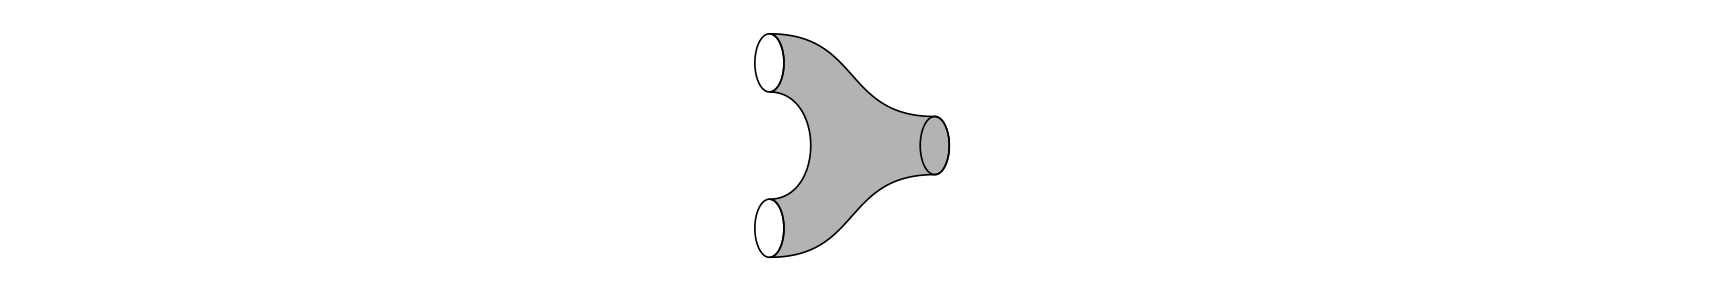
\includegraphics[width=0.55\textwidth]{figure4-1.png}
  \caption{从两个 $S^{1}$ 的无交并到单个 $S^{1}$ 的配边。（原文 p.~50，Figure 4.1）}
  \label{fig:4-1}
\end{figure}

这给出场的一个对应：
\begin{equation}\tag{4.35}
\begin{array}{cc}
\multicolumn{2}{c}{\cF(M)}\\[4pt]
\swarrow & \searrow\\[2pt]
\cF(\partial M_{\mathrm{in}}) & \cF(\partial M_{\mathrm{out}})
\end{array}
\end{equation}

% [Tutor Note: (4.35) 原书是一个交换图：$\cF(M)$ 在上，两条斜箭头分别指向
% $\cF(\partial M_{\mathrm{in}})$ 与 $\cF(\partial M_{\mathrm{out}})$。这里用
% \texttt{array} 重排，保留原编号；箭头方向与原图一致（都是“限制到边界”）。]

泛函 $e^{-S(\varphi)/\hbar}\mathcal{D}\varphi$ 生活于 $\cF(M)$ 之上，于是我们
得到一个积分变换：先拉回，乘以这个泛函，再积分（推出）。

这个积分变换给出 $\cH_{\mathrm{in}}$ 与 $\cH_{\mathrm{out}}$ 之间的算子 $Z(M)$，
其中
\begin{equation}\tag{4.36}
\cH_{\mathrm{in}}=\text{$\cF(\partial_{\mathrm{in}})$ 上的泛函},
\end{equation}
而
\begin{equation}\tag{4.37}
\cH_{\mathrm{out}}=\text{$\cF(\partial_{\mathrm{out}})$ 上的泛函}.
\end{equation}
于是
\begin{equation*}
\bigl(Z(M)(f)\bigr)(\varphi_{\mathrm{out}})
=\int_{\varphi|_{\partial \mathrm{out}}=\varphi_{\mathrm{out}}}f(\varphi|_{\partial \mathrm{in}})\,e^{-S(\varphi)/\hbar}\mathcal{D}\varphi
=\pi_{\mathrm{out}*}\Bigl(\pi^{*}_{\mathrm{in}}(f)\,e^{-S(\varphi)/\hbar}\mathcal{D}\varphi\Bigr).
\end{equation*}
这个算子就是\term{时间演化算子}{time evolution operator}。

\begin{srcrem}{17}（Hamilton 形式与 Lagrangian 形式）
在 Hamilton 形式中，我们从 Hilbert 空间 $\cH$ 出发，它附着在一个时间切片上。
然后还应当给出一个 Hamilton 算子 $H$，此时时间演化由算子 $e^{iTH/\hbar}$ 给出。
之后我们有一个可观测量的代数，并做各种测量。

另一方面，在 Lagrangian 形式中，我们从场空间与作用量出发。Lagrangian 表述非常
灵活，因为它允许我们定义这些推出—拉回算子，而 Hamilton 形式中的 Hilbert 空间
与时间演化算子（即 Hamilton 量）正是由此恢复出来的。
\end{srcrem}

\begin{srcex}{27}
一维量子场论就是量子力学。设 $X$ 是黎曼靶空间。那么场空间可能是
$\cF(\R)=\mathrm{Maps}(\R,X)$。$S$ 的临界点将是 $X$ 中的测地线。Hilbert 空间是
\begin{equation}\tag{4.38}
\cH=L^{2}(\mathrm{Maps}(\mathrm{pt},X))=L^{2}(X),
\end{equation}
而 Hamilton 量是 Laplace 算子 $\Delta$。
\end{srcex}

要把这一切严格化需要大量的工作。我们也不想使用任何微扰技术，因为我们并不
一定希望 $\hbar$ 很小。我们将把它当作示意性的指南，并形式地过渡到拓扑情形。

\section{量子 Maxwell 理论}
\begin{sectionkey}
四维 $U(1)$ 规范理论的经典作用量由 Yang--Mills 项与拓扑项
$\theta\int F\wedge F$ 组成；在 $M^{4}=M^{3}\times\R$ 上，Hilbert 空间是
$L^{2}(\cC(M^{3}))$，而 $\cC(M^{3})$ 按 $\Lambda=H^{2}(M,\Z)$、平坦联络环面 $T$
与向量空间 $V$ 分裂。't Hooft 算子实现 $\Lambda$ 的平移，Wilson 算子实现 $T$ 的
特征，二者分别对应磁与电的测量。
\end{sectionkey}

我们考虑一个四维量子场论。$4$-流形 $M^{4}$ 上的场空间由带联络 $d+A$ 的
$U(1)$-丛组成（$A$ 是电磁势），模去规范等价，即模去规范变换的作用。

经典运动方程是 Maxwell 方程：
\begin{equation}\tag{4.39}
\begin{cases}
dF=0\\
d\star F=0
\end{cases},
\end{equation}
其中 $F$ 是曲率。于是我们得到作用量
\begin{equation}\tag{4.40}
S=\frac{g}{2\pi i}\int_{M}F\wedge\star F+\theta\int_{M}F\wedge F.
\end{equation}

第二项中的积分只是在计算线丛的 $c_{1}^{2}=p_{1}$。这一项
\footnote{原文此处有旁注：“constants?”（是常数吗？）。}被称为\term{拓扑项}{topological term}。

% [Tutor Note: (4.40) 的归一化是 Maxwell 理论中最容易搞混的地方。通常写
% $S=\frac{1}{4e^{2}}\int F\wedge\star F+\frac{i\theta}{8\pi^{2}}\int F\wedge F$；
% 作者把 Yang--Mills 系数记成 $\frac{g}{2\pi i}$、把拓扑项系数记成 $\theta$，
% 这只是把 $g,\theta$ 吸收进定义。要点是：$\int F\wedge F$ 只依赖线丛的同构类，
% 因而在连续形变下不变（这就是它被称为“拓扑项”的原因）；在 $U(1)$ 情形它等于
% $c_{1}^{2}=p_{1}$ 的积分，取整数值，故 $\theta$ 以 $2\pi$ 为周期。]

想法是：Hilbert 空间附着在一个特定的时间切片上。于是假设可以写成
$M^{4}=M^{3}\times\R$，此时 Hilbert 空间是
\begin{equation}\tag{4.41}
\cH=L^{2}\bigl(\cC(M^{3})\bigr)
\end{equation}
其中 $\cC(M^{3})$ 表示 $M^{3}$ 上带联络的线丛模规范变换所得的集合。
$\cC(M^{3})$ 是一个交换 Lie 群，并且有一个到可能线丛同构类的格的映射：
\begin{equation}\tag{4.42}
\cC(M^{3})\xrightarrow{\ c_{1}\ }\Lambda=H^{2}(M,\Z),
\end{equation}
此外它还有一个由平坦联络构成的子环面：
\begin{equation}\tag{4.43}
T=\{\text{平坦联络}\}\simeq H^{1}(M,\R/\Z=U(1))\simeq BH^{1}(M,\Z)\to\cC(M^{3}),
\end{equation}
其中 $U(1)$ 取离散拓扑。于是 $\cH$ 的最后一个因子由一个无穷维向量空间 $V$
给出。也就是说，存在一个（非典范的）分裂 $\cC(M)\simeq\Lambda\times T\times V$。

% [Tutor Note: (4.43) 中出现的 “$BH^{1}(M,\Z)$” 在书中没有定义，$B$ 记号很
% 可能是笔误或作者自己的速记。数学上应读作 $T\simeq\Hom(H_{1}(M),\R/\Z)
% \simeq H^{1}(M,\Z)\otimes_{\Z}\R/\Z$；若坚持 $U(1)$ 取离散拓扑，则 $T$ 成为
% 一个无穷离散群，“环面”的说法只在通常拓扑下成立。]

\subsection{算子}
\label{sec:4-5-1}

现在我们要在 $\cH$ 上辨认出一些从这套设定中自然出现的算子（即可观测量）。
首先要说的是，$\cH$ 有一个由 $\Lambda=H^{2}(M,\Z)$ 给出的显然分次。这已经挑出了
一些算子，例如告诉你处在哪个连通分支上。这就是磁通量，所以说这是按磁通量的
分次。

\subsection*{Dirac／'t Hooft 算子}

$\Lambda$ 也作用在 $\cH$ 上，给出 \emph{'t Hooft 算子}。
\footnote{严格说来，'t Hooft 算子是这些东西的非阿贝尔推广。这些算子实际上与
Dirac 单极子有关，但“Dirac 算子”一词早已另有含义，那样叫会造成混淆。}
如果已经选定了分裂 $\cC(M)\simeq\Lambda\times T\times V$，那么这个作用就只是平移。
也就是说，这些算子平移磁通量。回忆通量大致记录了所包围的单极子数目。所以
物理上这些算子产生磁单极子。

更精确地说，设 $\gamma$ 是 $M$ 中的简单闭曲线。注意它定义了一个类
\begin{equation}\tag{4.44}
[\gamma]\in H_{1}(M,\Z)\simeq H^{2}(M,\Z)\simeq\Lambda.
\end{equation}
相应的算子如下所述地沿 $\gamma$ 引入一个单极子。想法是：$\gamma$ 位于
$M^{3}\times I$ 中某个特定的时间切片上，而我们研究的是 $M\times I$ 上沿
$\gamma$ 带一个单极子的电磁学，如图 \ref{fig:4-2}。

换言之，我们考虑场 $\cC(M\times I\setminus\gamma)$，即联络可能沿 $\gamma$ 有
奇点。于是我们把这个纽结挖去，这在我们的 4-流形上引入了一个新的边界分支：
纽结的环绕（纽结管状邻域的边界），它看起来像 $S^{2}\times S^{1}$。然后我们可以
考虑在这个边界上具有特定积分的联络。特别地，我们可以要求
\begin{equation}\tag{4.45}
\frac{1}{2\pi i}\int_{S^{2}}F=1.
\end{equation}
把所得的场空间记作
\begin{equation}\tag{4.46}
\cC(M\times I\setminus\gamma)_{c_{1}=1}.
\end{equation}
注意，物理上这就是说曲面 $S^{2}\times S^{1}\subset M^{3}\times I$ 包含磁荷 1。
数学上我们看到的是：我们无法把这个联络延拓过这条曲线。物理上我们看到的是
沿着这条曲线的一个单极子。

\begin{figure}[htbp]
  \centering
  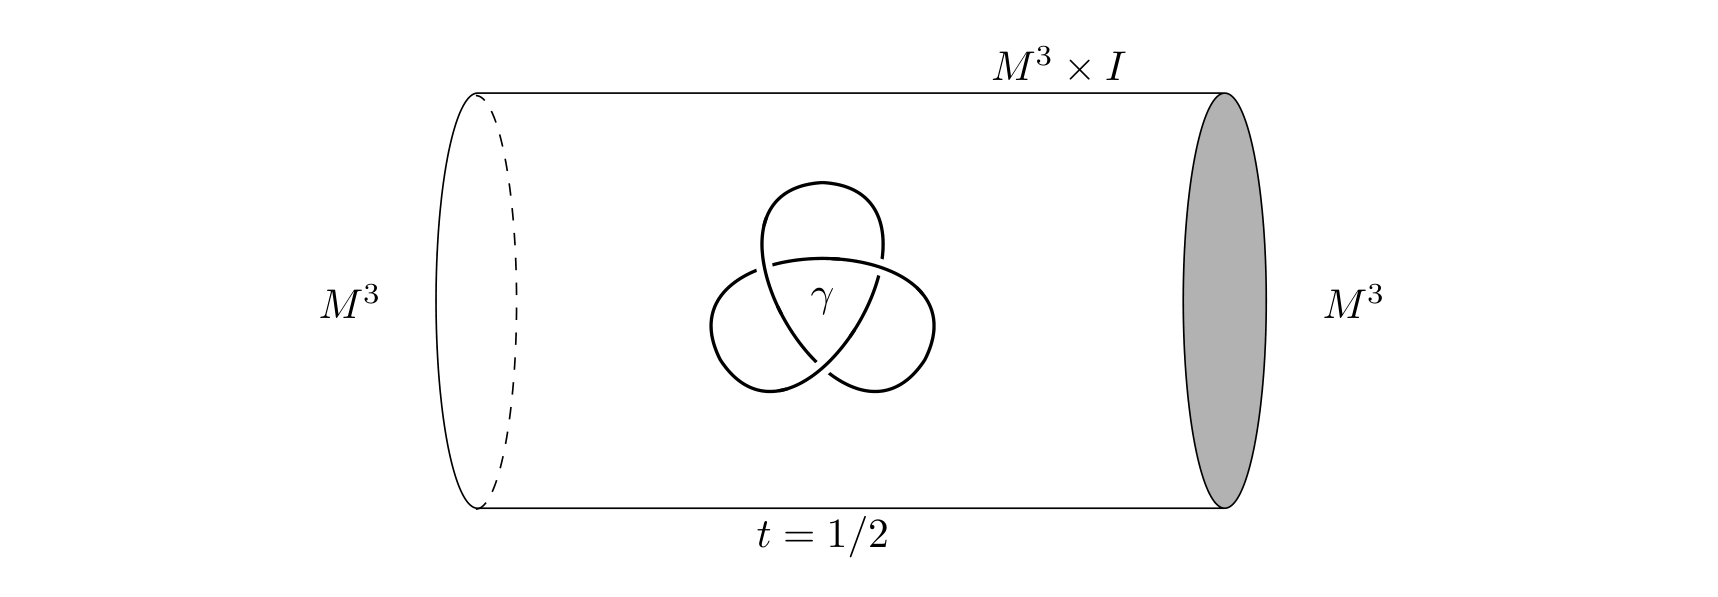
\includegraphics[width=0.55\textwidth]{figure4-2.png}
  \caption{环路 $\gamma$ 位于 $M^{3}\times I$ 的某个时间切片中，比如 $t=1/2$。
  我们可以把它挖去，所得 4-流形上的场可能沿 $\gamma$ 出现奇点；要求绕 $\gamma$
  的一个邻域的边界积分等于 1，便给出 $\gamma$ 邻域内部具有受控奇点的场空间。
  物理上这沿着 $\gamma$ 引入一个磁单极子。（原文 p.~52，Figure 4.2）}
  \label{fig:4-2}
\end{figure}

真正的算子是这样定义的。4-流形 $M\times I\setminus\gamma$ 是从 $M^{3}$ 到自身
的配边，因此像往常一样定义了一个对应与积分变换（Feynman 路径积分）：
\begin{equation}\tag{4.47}
\begin{array}{c}
\begin{array}{ccc}
 & \cC(M\times I\setminus\gamma)_{c_{1}=1} & \\[4pt]
{\scriptstyle\pi_{\mathrm{in}}}\swarrow & & \searrow{\scriptstyle\pi_{\mathrm{out}}}\\[4pt]
\cC\bigl(M^{3}_{\mathrm{in}}\bigr) & & \cC\bigl(M^{3}_{\mathrm{out}}\bigr)
\end{array}\\[10pt]
\cH\xrightarrow{\ \pi_{\mathrm{out}*}\bigl(e^{-S(\varphi)/\hbar}\mathcal{D}\varphi\,\pi^{*}_{\mathrm{in}}(-)\bigr)\ }\cH
\end{array}
\end{equation}
物理上，这个算子把状态空间沿时间演化，在此期间沿 $\gamma$ 引入一个单极子，
然后再把它移除。数学上它把 Chern 类平移 $[\gamma]$，也就是说，它只是与一个
具有指定 Chern 类的平坦线丛做张量积
\begin{equation}\tag{4.48}
c_{1}=[\gamma]\in H^{2}(M,\Z).
\end{equation}

% [Tutor Note: (4.47) 的交换图在原文中由“顶空间 + 两个投影 $\pi_{\mathrm{in}},
% \pi_{\mathrm{out}}$ + 底部的两个 $\cH$”构成，底部水平箭头标出的是积分核
% $\pi_{\mathrm{out}*}(e^{-S/\hbar}\mathcal{D}\varphi\,\pi^{*}_{\mathrm{in}}(-))$；
% 这里用 \texttt{array} 重排，保留了全部箭头与编号。“挖去 $\gamma$ 后$c_1=1$”
% 意味着联络在环绕 $S^{2}\times S^{1}$ 上的积分非零，故不能延拓——这正是
% 't Hooft 算子作为“无序算子”的几何含义。]

\subsection*{Wilson 环路算子}

另一方面，还有更简单的可观测量，称为 \term{Wilson 环路算子}{Wilson loop operator}。
仍设 $\gamma\subset M$ 是简单闭曲线。它决定了 $\cC(M)$ 上的一个函数 $W_{\gamma}$：
\begin{equation}\tag{4.49}
W_{\gamma}\colon (\cL,\nabla)\mapsto \text{沿 }\gamma\text{ 的和乐}\in U(1)\subset\C.
\end{equation}
我们可以画与图 \ref{fig:4-2} 同样的图，但我们对它做的事情完全不同。我们仍然把
$\gamma$ 想成位于 $M\times I$ 内某个时间切片上。现在，随着时间演化，我们做沿
$\gamma$ 的和乐测量。所以这与例 25 中局部算子的例子是同一类测量，只不过现在
测量是沿一个环路做的，因此称为线／环算子。这仍然给出一个对应与积分变换，
只不过现在变换的核由函数 $W_{\gamma}$ 给出：
\begin{equation}\tag{4.50}
\begin{array}{c}
\begin{array}{ccc}
 & \cC(M\times I) & \\[4pt]
{\scriptstyle\pi_{\mathrm{in}}}\swarrow & & \searrow{\scriptstyle\pi_{\mathrm{out}}}\\[4pt]
\cC\bigl(M^{3}_{\mathrm{in}}\bigr) & & \cC\bigl(M^{3}_{\mathrm{out}}\bigr)
\end{array}\\[10pt]
\cH\xrightarrow{\ \pi_{\mathrm{out}*}\bigl(W_{\gamma}\,\pi^{*}_{\mathrm{in}}(-)\bigr)\ }\cH
\end{array}
\end{equation}
要点是：我们可以把联络空间上的函数乘以这个函数 $W_{\gamma}$。所以按照我们
呈现 Hilbert 空间的方式，这些 Wilson 算子已经被对角化了。

Wilson 环路 $W_{\gamma}$ 是平坦联络空间作用的本征函数：
\begin{equation}\tag{4.51}
T=\cC_{\flat}(M)\simeq H^{1}(M,U(1)).
\end{equation}
它通过张量积作用在 $\cC(M)$ 上，因此也作用在 $L^{2}(\cC(M))$ 上。本征值由沿
$\gamma$ 的单值性给出：给定一个平坦联络（$H^{1}(M,U(1))$ 的元素），取沿
$\gamma$ 的单值性便典范地得到 $U(1)$ 的一个元素，而这正是在做 Fourier 级数。
这些 $W_{\gamma}$ 就是这个环面 $T$ 的特征。

\subsection{电磁对偶}
\label{sec:4-5-2}

注意，当我们研究 't Hooft 算子时，我们关注的是格的作用，并且有按磁通量的分次。
现在我们关注环面作用，并且可以对角化。这给出按 $T$ 的特征的分解，而这些特征
构成格 $H^{2}(M,\Z)$：
\begin{equation}\tag{4.52}
\cH=\bigoplus_{e\in H^{2}(M,\Z)}\cH_{e},
\end{equation}
这可以解释为按电通量的分次。

从磁分次过渡到电分次，恰好是对场空间的环面部分做 Fourier 变换。一般说来，
电磁对偶可以看成在我们场的 Lie 群上做 Fourier 级数。它具体地识别出
\begin{equation}\tag{4.53}
L^{2}\bigl(\cC_{U(1)}(M)\bigr)\simeq L^{2}\bigl(\cC_{U(1)^{\vee}}(M)\bigr),
\end{equation}
其中左边是 $F$ 侧，右边是 $\star F$ 侧。这个群总是分裂为格、环面与向量空间
（我们忽略最后一个）。$F$ 侧与 $\star F$ 侧分别对应如下分裂：
\begin{equation}\tag{4.54}
\Lambda_{B}\times T_{E}\times\mathrm{Vect}
\qquad\qquad
\Lambda_{E}\times T_{B}\times\mathrm{Vect}.
\end{equation}
$\Lambda_{B}$ 是磁通量的格，$T_{B}$ 是它的对偶环面，$\Lambda_{E}$ 是电通量的格，
$T_{E}$ 是它的对偶环面。在 $F$（左）侧，Wilson 环路算子被对角化；在 $\star F$
（右）侧，'t Hooft 算子被对角化。类似地，磁的 $b$ 分次变成电的 $e$ 分次。

% [Tutor Note: (4.53) 这个“等式”只在忽略向量空间因子 $V$ 的意义下成立：两边
% 的 $L^{2}$ 都含有同一个 $L^{2}(V)$ 因子，作者把它略去。真正的内容是
% Pontrjagin 对偶 $L^{2}(T)\simeq L^{2}(\Lambda^{\vee})$，以及
% $L^{2}(\Lambda)\simeq L^{2}(T^{\vee})$，即 Fourier 变换交换 $\Lambda$ 与 $T$。
% 把 $\Lambda_B\times T_E$ 与 $\Lambda_E\times T_B$ 对照 (4.54)，就能看出
% “$F$ 侧对角化 Wilson、$\star F$ 侧对角化 't Hooft” 的含义。]

\section{二维中的阿贝尔对偶}
\begin{sectionkey}
二维的电磁对偶就是 T-对偶（镜像对称）。场空间
$\mathrm{Map}(S^{1},S^{1}_{R})$ 是交换 Lie 群，Hilbert 空间
$L^{2}$ 的分解按绕数由 $H^{1}(S^{1},\Z)$ 分级；对偶理论以
$R\leftrightarrow1/R$ 的靶空间出现，其分级改由 $H^{0}(S^{1},U(1))$ 给出，
两套算子（'t Hooft 型与 Wilson 型）在对偶下互换。
\end{sectionkey}

回忆这被称为 T-对偶，或镜像对称。场空间是 $\mathrm{Map}(M,S^{1})$，或者更一般地
映入某个环面 $T$。我们在 $S^{1}$ 上的 Hilbert 空间 $\cH$ 于是是
\begin{equation}\tag{4.55}
L^{2}\bigl(\mathrm{Map}(S^{1},S^{1}_{R})\bigr).
\end{equation}
注意 $\mathrm{Map}(S^{1},S^{1})$ 在逐点乘法之下又是一个交换 Lie 群，即我们用
的是靶空间的群结构而非源空间的。这里也有一个到格的映射：它按
$H^{1}(S^{1},\Z)$ 分次，这是通过取绕数给出的。

对偶地，我们可以研究：
\begin{equation}\tag{4.56}
L^{2}\left\langle \mathrm{Maps}\left\langle S^{1},(S^{1}_{R})^{\vee}=S^{1}_{1/R}\right\rangle\right\rangle.
\end{equation}
它按 $H^{0}(S^{1},U(1))$ 分次，与上面的分次对偶。我们有一个由平移绕数给出的
算子（'t Hooft 算子的类似物），以及由在一点取值给出的算子（Wilson 算子的
类似物），而对偶交换它们。

% [Tutor Note: (4.55)--(4.56) 中“$S^{1}_{R}$”表示半径 $R$ 的圆。T-对偶的
% 标准陈述是：半径 $R$ 的圆上的自由玻色子等价于半径 $1/R$（在 $\alpha'=1$
% 的单位下）的圆上的自由玻色子，同时把动量模与绕数模互换。这里的分级
% $H^{1}(S^{1},\Z)=\Z$（绕数）与 $H^{0}(S^{1},U(1))$（取值）正是这一互换的
% 代数表现。原文用双重尖括号 $\langle\langle\cdots\rangle\rangle$ 排版，是一个
% 排版习惯，不影响含义。]

\section{拓扑量子力学／量子场论}
\begin{sectionkey}
量子力学之所以难，是因为要处理分析。Witten 的超对称技巧把
$L^{2}(X)$ 换成微分形式 $\Omega^{\bullet}(X)$，并加入 de Rham 微分 $Q=d$ 与
$Q^{*}=d^{*}$，使得 $H=[Q,Q^{*}]$，于是 $H$ 在 $Q$-上同调上为零：
时间被“导出地”杀死了，剩下的只是 $X$ 的上同调。
\end{sectionkey}

想法是：量子力学之所以难，是因为它涉及分析。在通常的量子力学中，我们从一点
出发，附着上一个 Hilbert 空间 $\cH$。然后对一个长度为 $T$ 的区间，我们附着上
酉时间演化算子
\begin{equation}\tag{4.57}
e^{iTH/\hbar}.
\end{equation}
在\term{拓扑量子力学}{topological quantum mechanics}（TQM）中，我们想杀死时间，
即我们希望 $H=0$。最朴素的解释方式是限制到基态。但闭流形上不存在非常值的
有界调和函数。所以这样一来我们把整个理论都杀死了。

Witten [Wit82] 引入了如下技巧，通过\term{超对称}{supersymmetry}（SUSY）
在导出的意义下杀死时间。设 $X$ 是黎曼流形。我们不用 $L^{2}(X)$，而是把
Hilbert 空间扩充为 $L^{2}$ 微分形式，即我们加入新的场，于是得到一个由超 Lie 群
给出的更大对称群。现在考虑：什么作用在微分形式上？首先是 Laplace 算子
$H=\Delta$。我们还有 de Rham 微分 $Q=d$ 及其伴随 $Q^{*}=d^{*}$。还有一个给出
$\Z$-分次的 $U(1)$ 作用。这套算子称为 $\mathcal{N}=1$ 超对称代数。于是我们有
算子 $H$（次数 0）、$Q$（次数 1）与 $Q^{*}$（次数 $-1$）。这些算子大多交换：
\begin{equation}\tag{4.58}
[Q^{*},Q^{*}]=[Q,Q]=0,
\end{equation}
\begin{equation}\tag{4.59}
[Q,H]=[Q^{*},H]=0,
\end{equation}
除了
\begin{equation}\tag{4.60}
[Q,Q^{*}]=H.
\end{equation}
$[Q,Q]=0$ 可以解释为 $d^{2}=0$。另一个关系是
\begin{equation}\tag{4.61}
\Delta=dd^{*}+d^{*}d,
\end{equation}
它说的是 $Q^{*}$ 给出从 $H$ 到 $0$ 的一个同伦。特别地，这意味着在
$Q$-上同调上，$H$ 的作用为 0。

于是我们加入了新场，得到了更大的对称代数。这个代数中的一个算子是平方为零的
奇算子，我们称之为微分。在相应的上同调上，$H$ 为零。所以我们在导出的意义下
杀死了时间。于是拓扑量子力学给 $X$ 附着上复形
\begin{equation}\tag{4.62}
\bigl(\Omega^{\bullet}(X),d\bigr),
\end{equation}
或者 $H^{*}(X)$。在第一种情形 $H$ 同伦于 0，在后一种情形 $H=0$。这就是从
量子力学中恢复 de Rham 上同调的方式。

% [Tutor Note: 这里“杀死时间”的准确含义是：在 $Q$-上同调（即把 $Q$-恰当形式
% 视为零）中，$H=[Q,Q^{*}]$ 作用为零，于是时间演化 $e^{iTH/\hbar}$ 在同调上
% 变成恒等。注意 $[Q,Q^{*}]=H$ 的符号依赖于 $Q^{*}$ 取 $d^{*}$ 还是 $-d^{*}$；
% 若取 $Q^{*}=-d^{*}$，则右边多一个负号，但“在 $Q$-上同调上 $H=0$”的结论不变。]

我们将永远不处理真正意义上的量子场论。相反，我们要做的是这种拓扑扭转。注意在
这套设定中，理论只拓扑地依赖于 $X$。结论就是：我们正在杀死对黎曼度量的依赖，
这会让日子好过得多。

\begin{flushright}\small 第 8 讲；2021 年 2 月 11 日\end{flushright}

\section{拓扑量子力学}
\begin{sectionkey}
TQM 的两种实现：A-型取 $(\Omega^{\bullet}(X),d)$，得上同调
$H^{\bullet}_{dR}(X)$；B-型取 $(\Omega^{0,\bullet}(X),\bar\partial)$，得
Dolbeault 上同调 $H^{0,*}(X)$。进一步还有 $\mathcal{N}=2$（Kähler 流形，
Lefschetz $\mathrm{SL}_{2}$ 作用）与 $\mathcal{N}=4$（超 Kähler 流形，
$\mathrm{Spin}(5)$ 作用）的版本。
\end{sectionkey}

\begin{flushright}\small 〔课次过渡〕\end{flushright}

形式地建立这套东西的方式是：有一个 $d=1$、$\mathcal{N}=1$ 的超对称代数作用在
$\cH$ 上。$d=1$ 意味着我们在做量子力学，而 $\mathcal{N}=1$ 只是说超对称的量
最少。

TQM 有两种自然的实现。第一种是 \emph{A-型} TQM。取 $X$ 为黎曼流形，那么
Hilbert 空间由微分形式组成：
\begin{equation}\tag{4.63}
\cH=\Omega^{\bullet}(X),
\end{equation}
Hamilton 量 $H=\Delta$ 是 Laplace 算子，$Q=d$ 是 de Rham 微分，而
$Q^{*}=d^{*}$ 是关于度量的伴随。分次是形式上的通常分次，上同调是
\begin{equation}\tag{4.64}
H^{\bullet}(\cH)=H^{\bullet}_{dR}(X).
\end{equation}

还有另一种实现，称为 \emph{B-型} TQM。此时取 $X$ 为复流形。Hilbert 空间是
\begin{equation}\tag{4.65}
\cH=\Omega^{0,\bullet}(X),
\end{equation}
即含 $\bar\partial$ 的形式。SUSY 算子由 $Q=\bar\partial$、$Q^{*}=\bar\partial^{*}$
与 $H=\Delta_{\bar\partial}$ 给出。上同调是 Dolbeault 上同调：
\begin{equation}\tag{4.66}
H^{0}(\cH)=H^{0,*}(X)=R\Gamma(\cO_{X}).
\end{equation}

这两种都是 1 维 $\mathcal{N}=1$ 超对称代数的实现。还有
$\mathcal{N}=2$ TQM。一个这样的例子来自研究 Kähler 流形 $X$。Hilbert 空间
仍然是微分形式：
\begin{equation}\tag{4.67}
\Omega^{\bullet,\bullet}(X).
\end{equation}
它是双分次的，而不像之前那样只有一个分次；它带有一批算子，例如
$\partial$、$\bar\partial$、$\partial^{*}$ 与 $\bar\partial^{*}$。
Kähler 恒等式告诉我们相应的 Laplace 算子相等：$\Delta_{\bar\partial}=\Delta_{d}$。

对数学家而言，有下面这个深刻的定理。我们有一个 $\mathrm{SU}(2)$ 在
$\Omega^{\bullet,\bullet}(X)$ 上的作用，可以把它想成来自复化
$\mathrm{SU}(2)\subset \mathrm{SL}_{2}\C$。这些就是 Lefschetz 算子。对角部分
给出上同调分次，然后有一个提升算子（与 Kähler 形式作交）和一个下降算子。
数学上这是关于 Kähler 流形整体上同调的一个非常深刻的陈述（硬 Lefschetz 定理）。
物理上这是在计算什么样的超对称代数作用在我们的 Hilbert 空间上，而这个
$\mathrm{SU}(2)$ 作用就是 R-对称。要点在于我们找到了一个很大的超对称代数。

$\mathcal{N}=1$ 超对称代数编码了黎曼流形的 Hodge 理论。这个 $\mathcal{N}=2$
超对称代数编码了复 Hodge 理论。还有 $\mathcal{N}=4$ TQM。此时我们研究紧超
Kähler 流形 $X$ 上的微分形式：$\Omega^{\bullet}(X)$。超 Kähler 情形下 Lefschetz
$\mathrm{SL}_{2}$ 作用的类似物是 $\mathrm{Spin}(5)$ 的作用。想法是：若把所有
Lefschetz $\mathrm{SL}_{2}$ 拼在一起，就得到一个 $\mathrm{Spin}(5)$。这是一个
我们不会写下来的超 Lie 群的一部分。从物理的观点看，这只是在研究这个流形上的
粒子理论时，对“周围坐着哪些算子”做的一个自然计算。

\begin{srcrem}{18}
还有 $\mathcal{N}=8$ 超对称。这些不同的超对称代数实际上是按存在的奇算子
（又称超荷 $Q$）的数目来区分的。例如 $\mathcal{N}=1$ 有两个，
$\mathcal{N}=2$ 有四个，$\mathcal{N}=4$ 有八个，而 $\mathcal{N}=8$ 有十六个。
\end{srcrem}

% [Tutor Note: 原文末句作 “$\mathcal{N}=8$ had 16”，时态 “had” 是笔误，
% 应为 “has”。另外“奇算子个数 = $2\mathcal{N}$”这一计数只在
% $\mathcal{N}\le 4$ 时与通常的物理约定一致；对 $\mathcal{N}=8$，超荷通常
% 计入其反粒子共轭，实际独立超荷数会因维数约化约定而不同，阅读时以原文的
% 计数为准即可。]

% [Tutor Note: (4.66) 中 $R\Gamma(\cO_{X})$ 的写法只在 $X$ 紧合（例如射影）
% 时才与 $H^{0,*}(X)$ 同构；一般复流形上应写作 $H^{0,*}_{\bar\partial}(X)$
% 与 $R\Gamma(\cO_X)$ 的导出范畴对象，而不是相等。作者在此处把
% “$H^{0}(\cH)$” 与 Dolbeault 上同调等同，是按紧 Kähler 情形书写的。]

TQM 乃至最终 TQFT 的一般哲学是：加入场，使得有一个大的超 Lie 群（超对称代数）
作用。我们要找两样东西：
\begin{enumerate}
\item Hamilton 量是恰当的：$H=[Q,-]$（即我们杀死了时间\footnote{即时间演化被
变得平凡。}），以及
\item $T=[Q,-]$，即度量依赖是恰当的（即我们杀死了几何）。
\end{enumerate}
\term{能量动量张量}{stress energy tensor} $T$ 是 QFT 中的一个对象，它衡量对
度量的依赖。数学上 $T$ 是等距不变性的导出版本。Costello--Gwilliam [CG17] 中
对此有很好的解释。

\subsection{拓扑 Maxwell 理论}
\label{sec:4-8-1}

我们想取光的量子理论（普通 Maxwell 理论），加入一些场，并找出超对称代数。
然后我们挑一个 $Q$ 并过渡到上同调。这将是一个 $\mathcal{N}=4$ 的 GL-扭转理论。
特别地，这个 $\mathcal{N}=4$ 意味着有大量超对称：将会有十六个超荷。

之前，我们的场空间由一个线丛与一个联络 $\nabla=d+A$ 的选择组成。现在我们要
加入：
\begin{itemize}
\item 流形上的一个 1-形式 $\sigma$（\term{Higgs 场}{Higgs field}），
\item 一个复标量 $u$，以及
\item 四个费米子（奇场）（我们不会太关注它们）。
\end{itemize}
Hilbert 空间原本是 $\cH=L^{2}(\cC(M))$。现在，在 A-扭转中，3-流形 $M^{3}$ 被
附着到这个空间的\emph{上同调}上：$H^{\bullet}(\cC(M))$。我们现在有一个大得多
的场空间，但在上同调层面这其实没有区别，因为引入这些新场并没有改变空间的
拓扑。但结果是：我们不要通常的上同调，我们要的是关于联络自同构等变的上同调，
即我们要的是：
\begin{align}
\cH&=H^{\bullet}(\text{联络}/\text{规范等价})\tag{4.68}\\
&=H^{\bullet}_{U(1)}\bigl(\cC(M)\bigr).\tag{4.69}
\end{align}
这是在联络空间上做 de Rham 意义下的拓扑量子力学。

% [Tutor Note: (4.69) 的下标 $U(1)$ 指对联络的自同构群（每点的 $U(1)$ 旋转，
% 即规范变换）取等变上同调。若只取通常上同调，$H^{\bullet}(\cC(M))$ 会因
% 每个连通分支上的 $BU(1)$ 因子而多出 $\C[u]$；等变化正是为了把规范自由度
% 正确地商掉，这一点在 (4.73) 中体现为显式的 $BU(1)$ 因子。]

还有另一个版本，称为 B-扭转。现在我们把场修改为把
\begin{equation}\tag{4.70}
\nabla+i\sigma=d+(A+i\sigma)
\end{equation}
看成 $\C^{\times}$-丛上的联络，而不是 $U(1)$-丛上的联络。附着到 $M^{3}$ 的
向量空间是 $\Loc_{\C^{\times}}(M)$ 上的 Dolbeault TQM。这只是说，该向量空间是
$\Loc_{\C^{\times}}(M)$ 上全纯函数的（某个导出版本）。

现在我们把 A-侧重新表述，以便与此前见过的东西联系起来。记
$\mathrm{Pic}(M)$ 为联络空间 $\cC(M)$ 的底层拓扑空间，即它不探测 $M$ 的黎曼
几何。$H^{0}(\mathrm{Pic}(M))$ 由联络空间 $\cC(M)$ 上的局部常值函数组成，即
\begin{align}
H^{0}\bigl(\mathrm{Pic}(M)\bigr)&=\C\bigl[\pi_{0}(\cC(M))\bigr]\tag{4.71}\\
&=\C\bigl[H^{2}(M,\Z)\bigr],\tag{4.72}
\end{align}
这正是我们之前在表 3.1 所总结的讨论中附着到 $M$ 上的同一个向量空间。这个空间
的完整上同调是：
\begin{equation}\tag{4.73}
H^{\bullet}\bigl(\mathrm{Pic}(M)\bigr)=H^{\bullet}\bigl(\Lambda\times T\times V\times BU(1)\bigr).
\end{equation}
之前我们只看到 $\Lambda=H^{2}(M,\Z)$，但现在我们将看到
\begin{itemize}
\item $T=H^{1}(M,U(1))$ 的上同调（一个外代数），
\item 向量空间对上同调没有贡献，但我们还会看到
\item $BU(1)$ 的上同调，它看起来像 $\C[u]$。
\end{itemize}
所以这就是做完拓扑扭转之后我们 Hilbert 空间的形状；在 B-侧也会有与这些额外的
外代数与对称代数部分相对应的因子。

% [Tutor Note: (4.72) 原文直接写作 $\C[H^{2}(M,\Z)]$，跳过了
% $\C[\pi_{0}(\cC(M))]$ 中“$\pi_0$ 由 $c_1$ 给出”这一步：由于
% $\cC(M)\to\Lambda$ 的纤维是连通的环面，$\pi_{0}(\cC(M))\cong\Lambda$。
% 另外注意 $\C[\Lambda]$ 是群代数，与 (4.75) 中
% $\C[T^{\vee}_{\C}]$ 的对偶关系正是 Fourier 变换。]

在 B-侧，我们看空间 $\Loc_{\C^{\times}}M$。在忽略一些导出因子之后，它看起来像
一个复环面 $\Loc_{\C^{\times}}M\simeq T^{\vee}_{\C}$，由那些分解为
\begin{equation}\tag{4.74}
\begin{array}{ccc}
\pi_{1}(M) & \longrightarrow & \C^{\times}\\[2pt]
\searrow & & \uparrow\\[2pt]
 & H_{1}(M) &
\end{array}
\end{equation}
的映射 $\pi_{1}(M)\to\C^{\times}$ 组成。$H_{1}(M)$ 看起来像 $\Lambda$
（由 Poincaré 对偶），所以这部分是格 $\Lambda$ 的对偶环面。回忆 Fourier 级数
识别出
\begin{equation}\tag{4.75}
\C\bigl[H^{2}(M,\Z)\bigr]
\qquad\text{以及}\qquad
\C\bigl[T^{\vee}_{\C}\bigr],
\end{equation}
而现在我们还有一些额外的（导出）因子，来自 $H^{2}(M,\C)$ 与 $H^{3}(M,\C)$。
$H^{2}(M,\C)$ 因子对应 A-侧的外代数因子，而 $H^{3}(M,\C)$ 因子对应 A-侧的
对称代数因子。

于是我们又一次有了 Fourier 变换的概念，它交换：
\begin{equation}\tag{4.76}
\Lambda=H^{2}(M,\Z)
\qquad\text{以及}\qquad
T^{\vee}_{\C}=|\Loc_{\C^{\times}}(M)|,
\end{equation}
而这原来只是 A-扭转与 B-扭转之间对偶的次数 0 部分，在那里我们有这个额外的
外代数与额外的对称代数。要旨：
\begin{itemize}
\item 规范群为 $T$ 的 A-扭转超 Maxwell 理论研究 $\mathrm{Pic}(M)$ 的拓扑，以及
\item 规范群为 $T^{\vee}$ 的超 Maxwell 理论的 B-扭转版本研究
$\Loc_{\C^{\times}}(M)$ 的代数几何。
\item 电磁对偶交换这两者。
\end{itemize}
总结见表 4.1。

\begin{srcrem}{19}
我们看了两种不同的扭转，即超对称代数的两种不同实现，也就是两个不同的荷。
我们也可以取这两者的任意线性组合，从而得到一个新的拓扑理论。换言之，这是
一个由量子 Maxwell 理论产生的 $\PP^{1}$ 族的可能拓扑理论。A、B 两种扭转则是
$\PP^{1}$ 的两个端点。在一端只剩下磁现象，在另一端只剩下电现象。
\end{srcrem}

\begin{table}[htbp]
  \centering
  \caption{超 Maxwell 理论的拓扑 A、B 扭转总结。（原文 p.~59，Table 4.1）}
  \label{tab:4-1}
  \small
  \begin{tabular}{ll}
    \toprule
    A-侧 & B-侧\\
    \midrule
    $\mathrm{Pic}$ 的拓扑 & $\Loc$ 的代数几何\\
    $\Lambda=H^{2}(M,\Z)$ & $T^{\vee}_{\C}=|\Loc_{\C^{\times}}(M)|$\\
    't Hooft 算子（按 $\gamma^{\vee}\in H^{2}(M,\Z)$ & Wilson 算子（乘以沿 $\gamma$\\
    \quad 平移格（磁通量）） & \quad 的单值性）\\
    产生磁单极子 & 产生电粒子\\
    磁侧 & 电侧\\
    \bottomrule
  \end{tabular}
\end{table}

% [Tutor Note: 表 4.1 原文以图像排版，这里按可用内容重排为 \texttt{tabular}，
% 以便检索与缩放；表中第 3 行“'t Hooft 算子 vs Wilson 算子”两栏内各有两行
% 说明，重排时用 \texttt{\textbackslash quad} 手动换行，语义与原文一致。]

\subsection{缺陷}
\label{sec:4-8-2}

电磁学中还有两种被称为\term{缺陷}{defect}的“物理操作”，我们将在拓扑层面
描述它们。它们相当于改变我们所考虑的场，例如引入奇点。

\subsection*{类时线缺陷}

我们要考虑的第一种缺陷是“类时”的 't Hooft 环／线。考虑点 $x\in M^{3}$。
于是我们可以考虑在 $x$ 处存在一个单极子的电磁学。数学上这意味着我们看联络
空间：
\begin{equation}\tag{4.77}
\mathrm{Pic}(M\setminus x)=|\cC(M\setminus x)|=\bigsqcup_{n}\mathrm{Pic}(M,nx),
\end{equation}
其中
\begin{equation}\tag{4.78}
\mathrm{Pic}(M,nx)=\{A\in\mathrm{Pic}(M\setminus x)\mid c_{1}=n\text{ 在 }x\text{ 处的球面上}\}.
\end{equation}
例如 $\cC(M,x)$ 是电荷 1 的分支。于是现在通过对 $\cC(M\setminus x)$ 做线性化
（取 $L^{2}$ 或 $H^{*}$），我们得到一个新的 Hilbert 空间。

对偶地（在 B-侧），我们有一个“类时”的 Wilson 环／线。对 $x\in M$，我们取
场为：
\begin{equation}\tag{4.79}
\Loc_{\C^{\times}}(M,x),
\end{equation}
即带有 $x$ 处纤维的一个平凡化的平坦 $\C^{\times}$ 联络。物理上这被解释为加入
一个\term{重}{heavy}带电粒子\footnote{“重”只是说我们不把它作为一个新场加进来
并与之一起做场论。}，但它在这一点上破坏了规范对称性。这个新的场空间
$\Loc_{\C^{\times}}(M,x)$ 是 $\Loc_{\C^{\times}}(M)$ 上的一个 $\C^{\times}$-丛：
\begin{equation}\tag{4.80}
\begin{array}{c}
\Loc_{\C^{\times}}(M,x)\\[2pt]
\downarrow\;{\scriptstyle\C^{\times}}\\[2pt]
\Loc_{\C^{\times}}(M)
\end{array}
\end{equation}
在 B-侧我们引入了一个额外的 $\C^{\times}$ 因子，而在 A-侧通过允许不同的电荷，
我们引入了一个额外的 $\Z$ 因子。Fourier 级数将识别这些因子：
\begin{equation}\tag{4.81}
H^{*}\bigl(\mathrm{Pic}(M\setminus x)\bigr)\simeq\C\bigl[\Loc_{\C^{\times}}(M,x)\bigr].
\end{equation}
这是电磁对偶的又一个实例：产生一个磁单极子，对应着产生一个带电粒子。

\subsection*{面缺陷}

另一类缺陷是\term{面缺陷}{surface defect}，也称为分歧，或引入螺线管。想法是：
我们有一根长管，外面绕着一圈导线，然后让电流通过它，这就在管内部产生一个磁场。
所以这是 3-流形 $M^{3}$ 的一个 1 维子空间，而把它与时间做乘积，$M\times I$，
就定义了一个曲面。

在 B-侧，这引入了电场的奇点，即我们的场是：
\begin{equation}\tag{4.82}
\Loc_{\C^{\times}}(M\setminus\beta).
\end{equation}
绕 $\beta$ 的和乐在 $H_{1}$ 中引入一个额外的 $\Z$ 因子。

磁的（A-侧）版本中，场由同一个联络空间 $\cC(M)$ 给出，但带有沿 $\beta$ 的
一个平凡化。这有什么用？沿一个环路的平凡化（或两个平凡化之差）是从
$\beta=S^{1}$ 到 $U(1)$ 的映射。它有绕数，所以我们得到 $\Z$ 多个场的连通分支。
这与 B-侧绕 $\beta$ 的和乐带来的额外 $\C^{\times}$ 对偶。所以这是 Fourier 级数
的又一个版本。具体地说，它识别出
\begin{equation}\tag{4.83}
\C\bigl[\Loc_{\C^{\times}}(M\setminus\beta)\bigr]\simeq H^{*}\bigl(\cC(M\text{ 沿 }\beta\text{ 平凡化})\bigr).
\end{equation}

% [Tutor Note: (4.81)、(4.83) 中 $\C[\Loc(\cdots)]$ 表示“该空间上的函数空间”
% （或函数空间的导出版本），并不是群代数；只有当 $\Loc$ 是离散群时才与群代数
% 重合。作者在 (4.72) 中 $\C[H^{2}(M,\Z)]$ 用的是群代数含义，两处记号相同而
% 含义不同，这是本书记号的一个陷阱。]
% [Tutor Note: 本节两类缺陷的物理含义不同：类时 't Hooft 线是“沿一条时间方向的
% 线插入磁流”，它改变 $\pi_{0}$（即 $c_{1}$），对应 A-侧增加 $\Z$；类时 Wilson
% 线是“沿一条时间方向的线做和乐测量”，它改变纤维的平凡化，对应 B-侧增加
% $\C^{\times}$。面缺陷（螺线管／分歧）则是沿一个曲面插入，二者的对偶由 Fourier
% 级数在“额外 $\Z$”与“额外 $\C^{\times}$”之间互换给出，与 (4.19)--(4.21) 中
% 的 Dirac 量子化是同一回事。]


% ============================================================================
%  第 5 章 类域论（原书 pp. 61--74）
%  译自 David Ben-Zvi, "Between Electric-Magnetic Duality and the Langlands Program"
%  Lecture notes by Jackson Van Dyke, UT Austin, Spring 2021.
% ============================================================================
\chapter{类域论}\label{ch:05}

\begin{keytakeaways}
数论（具体说是类域论）是与拓扑、物理并列的另一类对偶来源。对 数域 $F$，
理想类群 $\mathcal{C}\ell(F)=\mathrm{Pic}(\Spec\cO_{F})$ 是有限群，而（非分歧）
类域论把它与 Galois 群联系起来：$\mathcal{C}\ell(F)\simeq\Gal(F^{ur,ab}/F)$ 恰是
Hilbert 类域的自同构群。取特征便得到 Pontrjagin 对偶
$\Loc_{\GG_{m}}(\cO_{F})=\Hom(\mathcal{C}\ell(F),\C^{\times})$。在函数域情形，
$\mathrm{Pic}(C)$ 与“非分歧 Weil 群的交换化”$W_{C}^{ur,ab}$ 之间的对照（定理 2）
给出 $(\mathrm{Pic}(C))^{\vee}\simeq\Loc_{1}(C)$，即 $\mathrm{Pic}$ 上的函数与
$\Loc$ 上的函数之间的 Fourier 变换；此时 Hecke 算子 $L\mapsto L(x)$ 扮演
't Hooft 算子的角色，而 $\rho\mapsto\rho(\mathrm{Fr}_{x})$ 扮演 Wilson 算子的
角色。把 $\Spec\cO_{F}$ 看成（无向的）3-流形，这套对偶就是 Artin--Verdier
对偶。最后允许分歧：物理上挖去一个结与在结上做平凡化互为对偶；算术上温和分歧的
局部系统 $\Loc_{1}(C\setminus S)^{tame}$ 对偶于在 $S$ 上平凡化的线丛
$\mathrm{Pic}(C,S)$，而局部类域论 $\widehat{K^{\times}}\simeq\Gal^{ab}$ 说明这些
群在 $\F_{q}^{\times}$ 与 $\widehat{\Z}$ 上的商正好对应拓扑情形里看到的那些因子。
\end{keytakeaways}

拓扑与物理给了我们一类有趣的对偶陈述。数论，具体说是\term{类域论}{class field theory}
（CFT），是另一类来源。$\mathrm{Pic}$ 的拓扑（例如局部常值函数）仍将与 $\Loc$
的代数几何（例如代数函数）互换。但在这个语境中我们需要重新解释 $\mathrm{Pic}$
与 $\Loc$。

% [Tutor Note: 这里的缩写 CFT 指 class field theory（类域论），但在数学物理
% 文献中 CFT 通常指 conformal field theory（共形场论）。本书第四章讨论的是
% 拓扑场论与超对称，本章讨论的是类域论；阅读时务必按上下文区分这两个 CFT。]

设 $F/\Q$ 是数域。记 $\mathcal{C}\ell(F)$ 为\term{理想类群}{ideal class group}。
可以把它看成：
\begin{equation}\tag{5.1}
\mathcal{C}\ell(F)=\mathrm{Pic}(\Spec\cO_{F}),
\end{equation}
它由 $\Spec\cO_{F}$ 上的线丛组成，即秩 1 投射 $\cO_{F}$-模模同构。具体地说，
类群是
\begin{equation}\tag{5.2}
\mathcal{C}\ell(F)=\text{$\cO_{F}$ 的分式理想}\big/\text{主理想}.
\end{equation}
注意这是一个交换群。事实证明 $\mathcal{C}\ell(F)$ 还是有限群，其阶是 $F$ 的一个
重要不变量，称为\term{类数}{class number}。类域论的一般哲学是把类群与 Galois 群
联系起来。

\section{非分歧类域论}
\begin{sectionkey}
非分歧类域论把理想类群与 Galois 群的交换化等同起来：
$\mathcal{C}\ell(F)\simeq\Gal(F^{ur,ab}/F)=\Aut(\text{Hilbert 类域})$。取特征后，
$\Loc_{\GG_{m}}(\cO_{F})=\Hom(\mathcal{C}\ell(F),\C^{\times})=\mathcal{C}\ell(F)^{\vee}$，
这正是算术拓扑字典中“$\Spec\cO_{F}$ 像 3-流形”的 Poincaré 对偶，即
Artin--Verdier 对偶。
\end{sectionkey}

非分歧类域论识别出：
\begin{equation}\tag{5.3}
\C\bigl[\mathcal{C}\ell(F)\bigr]\simeq\C\bigl[\Loc_{\GG_{m}}(\cO_{F})\bigr].
\end{equation}
但我们需要明确在这个语境中 $\Loc$ 是什么。我们总可以把 $\Loc$ 想成由 $\pi_{1}$
的表示组成，也可以写成：
\begin{equation}\tag{5.4}
\pi_{1}(M)=\Aut\bigl(\widetilde{M}\bigr),
\end{equation}
其中 $\widetilde{M}$ 是 $M$ 的万有覆叠。在这个语境中我们有
\begin{equation}\tag{5.5}
\Gal(E/F)=\Aut_{F}(E),
\end{equation}
而万有覆叠的类似物是 $F$ 的\term{最大非分歧扩张}{maximal unramified extension}，
记作 $F^{ur}$。于是 $\pi_{1}$ 的类似物是
\begin{equation}\tag{5.6}
\pi_{1}^{\text{ét}}(\Spec\cO_{F})=\Gal(F^{ur}/F).
\end{equation}

% [Tutor Note: (5.3) 原文印作 “$\C[\mathcal{C}\ell(f)]$”，其中 $f$ 小写，
% 明显是 $F$ 的笔误。另外这里 $\C[-]$ 是“函数空间”的记号（更准确地说，
% 是对于有限群 $\mathcal{C}\ell(F)$ 的函数空间），与 (4.72) 中群代数的含义
% 相同；两边都是有限维的，因为 $\mathcal{C}\ell(F)$ 有限。]

\begin{figure}[htbp]
  \centering
  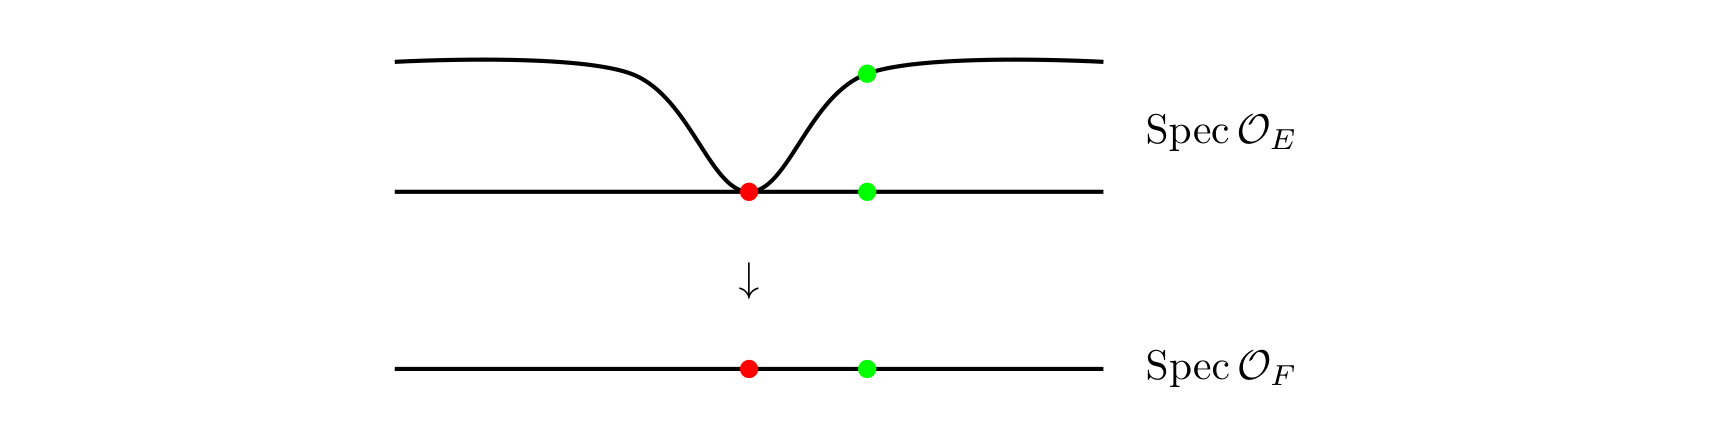
\includegraphics[width=0.72\textwidth]{figure5-1.png}
  \caption{一个在红点处分歧（左）、在绿点处非分歧（右）的扩张。（原文 p.~62，Figure 5.1）}
  \label{fig:5-1}
\end{figure}

% 说明：figure5-1.png 已包含整幅原图（上层 Spec O_E、中间竖直箭头、下层 Spec O_F）；
% figures/inline/p062_d1.png 只是同一图上半部分的放大裁剪，故此处不再重复插入。

我们取 $F^{ur}$，是因为我们要考虑 $\Spec\cO_{F}$ 的覆叠，而不是 $F$ 本身的
覆叠。我们说 $E/F$ 在素理想 $\mathfrak{p}$ 处\term{非分歧}{unramified}，如果
\begin{equation}\tag{5.7}
\cO_{E}\otimes_{\cO_{F}}\cO_{F}/\mathfrak{p}\;(=\cO_{E}/\mathfrak{p})
\end{equation}
是域的乘积，即它没有幂零元。想法是：有 $\Spec\cO_{E}$ 生活在 $\Spec\cO_{F}$
之上，而我们不希望出现图 \ref{fig:5-1} 那样的分叉。也就是说，如果看基中一点的
原像，我们希望得到域的乘积。如果出现幂零，那就说明该点处有某种有趣的几何，
我们现在想避开它。任意扩张在分歧点之外仍将扮演覆叠空间的作用。
$E/F$ 在 $\infty$ 处\term{非分歧}{unramified}，如果它们之间没有 $\C/\R$ 型的
扩张。例如 $F$ 是全虚的。想法是：与 $\R$ 做张量积对应于限制到无穷远处的邻域。
但这只是一堆 $\R$ 与 $\C$ 的拷贝：
\begin{equation}\tag{5.8}
\cO_{F}\otimes_{\Q}\R=\R^{r}\times\C^{s},
\end{equation}
然后我们要求从 $F$ 到 $E$ 的过程绝不涉及从 $\R$ 到 $\C$ 的扩张。

现在基础打好了，我们可以陈述：非分歧类域论告诉我们
\begin{equation}\tag{5.9}
\mathcal{C}\ell\simeq\Gal\bigl(F^{ur,ab}/F\bigr)=\Aut(\text{Hilbert 类域}),
\end{equation}
其中 \term{Hilbert 类域}{Hilbert class field} 是 $F$ 的最大交换扩张，且处处非分歧。

为了与此前所见的东西建立联系，我们应当研究这个 Galois 群的特征。也就是说，
一边我们有 $\mathrm{Pic}$ 的类似物 $\mathcal{C}\ell$，另一边 $\Loc$ 的类似物是：
\begin{equation}\tag{5.10}
\Hom\bigl(\Gal(F^{ur}/F),\C^{\times}\bigr).
\end{equation}
要点是：映入交换群的同态会分解到交换商上：
\begin{equation}\tag{5.11}
\Hom\bigl(\Gal(F^{ur}/F),\C^{\times}\bigr)
=\Hom\bigl(\Gal(F^{ur,ab}/F),\C^{\times}\bigr).
\end{equation}

\begin{srcrem}{20}
$\Gal(F^{ur}/F)$ 是 $\pi_{1}(\Spec\cO_{F})$ 的类似物，而
$\Gal(F^{ur,ab}/F)$ 是 $H_{1}(\Spec\cO_{F})$ 的类似物。所以这两个 $\Hom$ 空间
相等，类比于从 $\pi_{1}(\Spec\cO_{F})$ 出发的态射分解过它的交换化
$H_{1}(\Spec\cO_{F})$。
\end{srcrem}

% [Tutor Note: 这里“类似物”的层次要对齐：拓扑侧是
% $\pi_{1}\to H_{1}=\pi_{1}^{ab}$，算术侧是
% $\Gal(F^{ur}/F)\to\Gal(F^{ur,ab}/F)$。注意 (5.9) 已经用了交换化，
% 所以 (5.10)--(5.11) 的分解正是“特征只看见交换商”这一事实的特例；
% 反过来，这也说明单靠特征无法恢复非交换的 $\Gal(F^{ur}/F)$。]

于是由 (5.9)，这就是类群的 Pontrjagin 对偶：
\begin{align}
\Loc_{\GG_{m}}(\cO_{F})&=\Hom\bigl(\Gal(F^{ur}/F),\C^{\times}\bigr)\tag{5.12}\\
&=\Hom\bigl(\Gal(F^{ur,ab}/F),\C^{\times}\bigr)\tag{5.13}\\
&=\Hom\bigl(\mathcal{C}\ell(F),\C^{\times}\bigr)\tag{5.14}\\
&=\mathcal{C}\ell(F)^{\vee}.\tag{5.15}
\end{align}

\begin{srcrem}{21}
Artin--Verdier 对偶是 $\Spec\cO_{F}$ 上 Poincaré 对偶的类似物。这是我们建立
算术拓扑字典的基础，该字典说数域（或更确切地说 $\Spec\cO_{F}$）类比于
一个 3-流形。回忆对 3-流形而言 $\mathrm{Pic}$ 与 $\Loc$ 之间的对偶就是
Poincaré 对偶，而这个类域论的重述正是 Artin--Verdier 对偶的陈述。但
Artin--Verdier 对偶的建立依赖于类域论，所以这并不是用来证明类域论的方向。
\end{srcrem}

\begin{srcrem}{22}
算术拓扑字典告诉我们 $\Spec\cO_{F}$ 对应于一个 3-流形。结果表明它是一个
\emph{无向}的 3-流形。也就是说，对偶化对象不是常值对象。这种定向的缺失类比于
以下差别：
\begin{itemize}
\item $\Z/n$ 与单位根 $\mu_{n}$，
\item $\Q/\Z$ 与 $\mu_{\infty}$，
\item $\C^{\times}$ 与 $\GG_{m}$，等等。
\end{itemize}
结果表明，对偶化对象不是 $\Z$，而是 Tate 扭 $\Z(1)$（$\mu_{n}$ 相对于
$\Z/p\Z$ 的代数闭包）。在 Gauss 定律中，或者在计算线丛的 Chern 类时，
我们遇到过一些 $2\pi i$ 因子。它们正是由这一现象来解释的。
\end{srcrem}

% [Tutor Note: $\Z(1)=\varprojlim\mu_{n}$ 是 Tate 模，其“取向”相当于选取
% 一个相容的单位根系统；$\R$ 上的对应物是 $2\pi i\Z$。这就是为什么 (4.19)
% 中的 $b_{\Sigma}=\frac{1}{2\pi i}\int F$ 与 (5.80) 的 Lefschetz 对偶里
% 都会出现 $2\pi i$：算术侧用 $\Z(1)$ 代替 $\Z$，等价于在拓扑侧把常值系数
% 换成带 twist 的系数。原文说“$\mu_n$ with respect to the algebraic closure
% of $\Z/p\Z$”，准确说法应是“相对于 $\Spec\F_{p}$ 的代数闭包的 $p$-进 Tate 模”。]

把 $\Gal^{ur}$ 的特征与 $\mathcal{C}\ell^{\vee}_{F}$ 等同起来的结论是：我们得到
一个 Fourier 变换
\begin{equation}\tag{5.16}
\C[\mathcal{C}\ell_{F}]\simeq\C\bigl[\Loc_{1}(\Spec\cO_{F})\bigr],
\end{equation}
其中 $\Loc_{1}$ 定义为 $\Gal^{ur}$ 的特征。

\begin{flushright}\small 第 9 讲；2021 年 2 月 23 日\end{flushright}

\begin{srcex}{28}
若 $F=\Q$，则两边都是平凡的。
\end{srcex}

\section{函数域}
\begin{sectionkey}
在函数域情形，$\mathrm{Pic}(C)$（线丛模同构）与“非分歧 Weil 群的交换化”
$W_{C}^{ur,ab}$ 满足同样的三条性质：都满射到 $\Z$、都交换、且对每个 $k$-点有
截面。定理 2 断言它们在投射有限完备化上同构；取特征后得到
$(\mathrm{Pic}(C))^{\vee}\simeq\Loc_{1}(C)$，从而有 $\mathrm{Pic}$ 与 $\Loc$
之间的 Fourier 变换，Hecke 算子对应于 't Hooft 算子，Frobenius 的特征值对应于
Wilson 算子。
\end{sectionkey}

设 $C$ 是某个域 $k$ 上的光滑射影曲线。对它我们可以附着上\term{函数域}{function field}
$F=k(C)$，即 $C$ 上有理函数构成的域。我们也可以考虑 \term{Picard 群}{Picard group}
$\mathrm{Pic}(C)$，其 $k$-点由下式给出：
\begin{align}
\mathrm{Pic}(C)(k)&=\{\text{$C$ 上的线丛}\}/\sim\tag{5.17}\\
&=\{\text{局部自由秩 1 的 $\cO_{C}$-模}\}\tag{5.18}\\
&=\{\text{除子}\}/\{\text{主除子}\}\tag{5.19}\\
&=H^{1}(C,\cO^{\times})\tag{5.20}
\end{align}
最后一行我们用转移函数（即 Čech 上链）来刻画线丛。每个线丛都有一个\term{次数}{degree}，
它是整数。如果把线丛想成由和式 $\sum_{x\in C}n_{x}x$ 给出，那么这具体地由映射
\begin{equation}\tag{5.21}
\begin{array}{ccc}
\mathrm{Pic} & \xrightarrow{\ \deg\ } & \Z\\[2pt]
\sum_{x\in C}n_{x}x & \longmapsto & \sum n_{x}
\end{array}
\end{equation}
给出，它满射，其核为
\begin{equation}\tag{5.22}
0\to \mathrm{Jac}\to\mathrm{Pic}\to\Z\to 0,
\end{equation}
其中 $\mathrm{Jac}$ 是\term{Jacobi 簇}{Jacobian}，即次数为 0 的线丛。对任意
选定的 $x\in C$，我们都得到一份 $\Z x\hookrightarrow\mathrm{Pic}$，即这个扩张是
可裂的，且对曲线上每个点都有一个截面。

若 $k=\F_{q}$ 有限，这与我们从 $C$ 的（平展）基本群看到的东西类似。它不以 $\Z$
为商，而是以\term{投射有限完备化}{profinite completion}\footnote{回忆投射有限
完备化是所有有限商的逆向极限。} $\widehat{\Z}$ 为商：
\begin{equation}\tag{5.23}
\pi_{1}^{\text{ét}}(C)\twoheadrightarrow\widehat{\Z}=\pi_{1}^{\text{ét}}(\Spec k).
\end{equation}
想法是：曲线 $C$ 生活在 $\Spec k$ 之上，于是对 $\Spec k$ 的一个覆叠，我们可以
把它拉回成 $C$ 的覆叠 $\widetilde{C}$。这对应于从 $C$ 的基本群到 $\Spec k$ 的
基本群的映射。这与上面的情形看起来非常相似：$\mathrm{Pic}$ 以 $\Z$ 为商，
但有两个主要区别：
\begin{enumerate}
\item $\pi_{1}^{\text{ét}}$ 不是交换的，以及
\item $\widehat{\Z}$ 不是 $\Z$。
\end{enumerate}
我们可以用两种不同方式处理。第一件可做的事是把
$\pi_{1}^{\text{ét}}=\Gal^{ur}(F)$ 换成 $C$ 的\term{非分歧 Weil 群}{unramified Weil group}，
记作 $W_{C}^{ur}$。想法是我们想让 $\Spec k$ 看起来更像 $S^{1}$，于是把
$\widehat{\Z}$ 换成 $\Z$，而 $W_{C}^{ur}$ 就是 $\Z$ 在
$\pi_{1}^{\text{ét}}$ 中的原像：
\begin{equation}\tag{5.24}
\begin{array}{ccc}
\pi_{1}^{\text{ét}} & \longrightarrow & \widehat{\Z}\\[2pt]
\uparrow & & \uparrow\\[2pt]
W_{C}^{ur} & \longrightarrow & \Z
\end{array}
\end{equation}
另一件可做的事是过渡到交换化：$W_{C}^{ur,ab}$，它以 $\Z$ 为商：
\begin{equation}\tag{5.25}
W_{C}^{ur,ab}\twoheadrightarrow\Z.
\end{equation}
对每个点 $x\in C(k)$ 这个映射也有一个截面，正如上面 $\mathrm{Pic}$ 的情形。
一个点是映射 $x\colon\Spec k\to C$，几何上这给出一个映射
\begin{equation}\tag{5.26}
\widehat{\Z}=\pi_{1}^{\text{ét}}(k)\to\pi_{1}^{\text{ét}}(C),
\end{equation}
它就是相应的截面。图景是：$\Spec k$ 是圆的类似物，而 $C$ 是纤维化于其上的
3-流形的类似物。于是 $C$ 的一个 $k$-点就是一个截面，即 $C$ 中的一个环路。
总结一下，断言是：$\mathrm{Pic}$ 与 $W_{C}^{ur,ab}$ 二者都

% [Tutor Note: (5.24) 中 $W_{C}^{ur}$ 的定义是
% $W_{C}^{ur}:=(\pi_{1}^{\text{ét}})^{-1}(\Z)\subset\pi_{1}^{\text{ét}}$，
% 其中 $\Z\subset\widehat{\Z}$ 是自然包含。这个构造的意义在于：把
% $\Gal(\overline{\F}_{q}/\F_{q})\cong\widehat{\Z}$ 换成它的稠密子群 $\Z$
% （Frobenius 生成的子群），就得到“几何基本群 + Frobenius”的半直积结构；
% 这使 Weil 群成为比 $\pi_{1}^{\text{ét}}$ 更接近拓扑基本群的对象。]

\begin{itemize}
\item 满射到 $\Z$，
\item 交换，且
\item 对每个 $x\in C(k)$ 都有截面。
\end{itemize}

我们可以不改变有限域的图景，而改为改动 $\mathrm{Pic}$。回忆 $\mathrm{Pic}$ 是
$\Z$ 被 Jacobi 簇扩张，而后者在有限域上是有限群。因此 $\mathrm{Pic}$ 的所有
“无穷部分”都来自 $\Z$。于是我们可以把 $\mathrm{Pic}$ 换成它的投射有限完备化
$\widehat{\mathrm{Pic}}$。这样我们就得到一个对象：它满射到 $\widehat{\Z}$，
并且对每个点 $x\in C$ 有截面。无论如何，定理的内容就是它们匹配。

\begin{srcthm}{2}（非分歧类域论）
存在一个映射 $\mathrm{Pic}\to\pi_{1}^{\text{ét},ab}$，它在投射有限完备化上
是同构。等价地，我们有一个同构
\begin{equation}\tag{5.27}
\mathrm{Pic}\simeq W_{C}^{ur,ab},
\end{equation}
它保持取线丛次数的运算，并保持与 $x\in C$ 相关联的截面。
\end{srcthm}

% [Tutor Note: 定理 2 的准确含义是：$\mathrm{Pic}(C)$ 与
% $\pi_{1}^{\text{ét}}(C)^{ab}$ 的投射有限完备化同构，即
% $\widehat{\mathrm{Pic}(C)}\cong\pi_{1}^{\text{ét}}(C)^{ab}$；由于
% $\mathrm{Pic}$ 已是 $\Z$ 被有限群 $\mathrm{Jac}$ 的扩张，取完备化只是把
% $\Z$ 换成 $\widehat{\Z}$。这就是为什么 (5.27) 右边写 $W_C^{ur,ab}$：
% $W_C^{ur,ab}$ 正是以 $\Z$ 为商（而非 $\widehat\Z$）的那个版本。原文的
% “isomorphism on profinite completions” 一句容易误读成“两个群本身同构”，
% 实际上只是完备化后同构。另外，本章的定理编号是 “定理 2”“定理 3”，与章节号
% 无关（第 1 章的定理 1 未出现在本章），这是原书的全局编号方式，译文照原样保留。]

\begin{srcex}{29}
若 $C=\PP^{1}$，则两边都只是 $\Z$。对亏格更高的曲线这会更有趣。
\end{srcex}

现在我们要用更接近此前见过的 Pontrjagin 对偶的方式重新表述这一点。定理 2 蕴含
$\mathrm{Pic}$ 的特征与 $W_{C}^{ur,ab}$ 的特征相同，但一旦取特征，我们就无法
察觉交换化，所以
\begin{align}
\text{$\mathrm{Pic}$ 的特征}&\simeq\text{$W_{C}^{ur,ab}$ 的特征}\tag{5.28}\\
&\simeq\text{$W_{C}^{ur}$ 的特征}\tag{5.29}\\
&\simeq\text{$\pi_{1}^{\text{ét}}(C)$ 的特征}\tag{5.30}\\
&\simeq\text{$C$ 上秩 1 的局部系统}.\tag{5.31}
\end{align}
也就是说，$\mathrm{Pic}(C)$ 的 Pontrjagin 对偶是：
\begin{equation}\tag{5.32}
\bigl(\mathrm{Pic}(C)\bigr)^{\vee}\simeq\Loc_{1}(C).
\end{equation}
由此我们可以作出的一类陈述是：存在一个 Fourier 变换，把 $\mathrm{Pic}$ 上的
函数与 $\Loc$ 上的函数等同起来。

在 $\mathrm{Pic}$ 上的函数之中，我们有特征。特征条件，即要求
$\chi(gh)=\chi(g)\chi(h)$，等价于要求
\begin{equation}\tag{5.33}
\mu^{*}\chi=\pi_{1}^{*}\chi\boxtimes\pi_{2}^{*}\chi,
\end{equation}
其中
\begin{equation}\tag{5.34}
\begin{array}{ccc}
\mathrm{Pic}\times\mathrm{Pic} & \xrightarrow{\ \mu\ } & \mathrm{Pic}\\[2pt]
{\scriptstyle\pi_{1}}\swarrow & & \searrow{\scriptstyle\pi_{2}}\\[2pt]
\mathrm{Pic} & & \mathrm{Pic}
\end{array}
\end{equation}

% [Tutor Note: (5.33) 中 $\boxtimes$ 是外张量积：$\chi$ 是 $\mathrm{Pic}$ 上的
% 函数，$\pi_{1}^{*}\chi\boxtimes\pi_{2}^{*}\chi$ 是 $\mathrm{Pic}\times
% \mathrm{Pic}$ 上的函数。这是“乘法特征”的函子性表述，也可写成
% $\mu^{*}\chi=\chi\otimes\chi$。对一般（非交换）群，特征只对应一维表示，
% 这正是为什么下面只考虑交换的 $\mathrm{Pic}$。]

等价地，它们是 $\mathrm{Pic}$ 在自身上平移作用的本征函数。但 $\mathrm{Pic}$ 由
$\Z_{x}$（$x\in C$）生成，所以一个特征等同于 $\mathrm{Pic}$ 上的函数 $f$，它
对所有 $x\in C$ 的 $\Z_{x}$ 作用都是本征函数。具体地说，对 $x\in C$，这个作用
把 $\cL\in\mathrm{Pic}$ 送到线丛 $\cL(x)$，即 $\cL$ 在除子上多加了一个 $1\cdot x$。
成为本征函数意味着：
\begin{equation}\tag{5.35}
f(\cL(x))=\gamma_{x}\cdot f(\cL),
\end{equation}
其中 $\gamma_{x}$ 是一个数。

在这个 Fourier 变换下，这些本征函数应当变成 $\Loc$ 上类似 delta 函数的东西。
元素 $\rho\in\Loc$ 是一个表示：
\begin{equation}\tag{5.36}
\rho\colon\pi_{1}^{\text{ét}}\to e^{\times}
\end{equation}
其中 $e$ 是某个系数域（例如 $\C$）。那么 $f$ 是本征函数当且仅当
\begin{equation}\tag{5.37}
f(\cL(x))=\rho(\mathrm{Fr}_{x})\cdot f(\cL).
\end{equation}
想法是：一个局部系统对曲线上每个点给出一族本征值
$\gamma_{x}=\rho(\mathrm{Fr}_{x})$，即 $\rho\in\Loc$ 决定了 $\Z_{x}$（$x\in C$）
的本征值。

算子 $\cL\mapsto\cL(x)$ 是一个 \term{Hecke 算子}{Hecke operator}。它们扮演的是
第 4.5.1 节中 't Hooft／Dirac 单极子算子的角色：那些算子通过平移作用在
$H^{2}(M)\simeq\Lambda$ 上，并由环路 $\gamma\in H_{1}(M)$ 标记。回忆我们那时把
它想成 $H^{2}(M)=\pi_{0}(\mathrm{Pic})$。

另一方面，我们有第 4.5.1 节中的 Wilson 算子。对 3-流形 $M$，我们送
\begin{equation}\tag{5.38}
\Loc_{1}(M)\ni\rho\mapsto W_{\gamma}(\rho)=\rho\text{ 绕 }\gamma\text{ 的单值性}.
\end{equation}
现在我们要送
\begin{equation}\tag{5.39}
\Loc_{1}\ni\rho\mapsto\rho(\mathrm{Fr}_{x}).
\end{equation}
又一次，在所有这些情形中，我们都在把 $\mathrm{Pic}$ 的代数几何作为 $\Loc$ 的
拓扑的实现来研究，反之亦然。

\subsection{Loc}
\label{sec:5-2-1}

现在解释一点关于如何思考 $\Loc$ 的事情。在代数几何中，我们无法完全“接触”
$\pi_{1}$，因为我们只有有限覆叠。

\begin{srcex}{30}
考虑去心的仿射直线 $\bA^{1}\setminus\{0\}$。我们无法接触万有覆叠，因为它是
指数映射 $\exp\colon\bA^{1}\to\bA^{1}\setminus\{0\}$，而这不是代数函数。但我们
可以接触它的有限覆叠，因为 $t^{1/n}$ 是代数的。
\end{srcex}

于是我们首先可能研究的是形如
\begin{equation}\tag{5.40}
\pi_{1}\to\mu_{n}\subset\Q/\Z
\end{equation}
的映射。此外，当 $\operatorname{char}k=p$ 时，只有阶与 $p$ 互素的覆叠理论才
“如预期地”运作。所以我们需要选一个与 $p=\operatorname{char}k$ 不同的素 $\ell$，
然后可以研究映射
\begin{equation}\tag{5.41}
\pi_{1}\to\Z/\ell^{n}.
\end{equation}
但关于 $\ell$ 取逆向极限就得到 $\Z_{\ell}$，于是我们可以理解映入
$\Z_{\ell}$ 的表示；我们还可以向上张量，即沿
\begin{equation}\tag{5.42}
\Z/\ell^{n}\leftarrow\Z_{\ell}\subset\Q_{\ell}\subset\overline{\Q}_{\ell}
\end{equation}
提升表示。

结论就是：这引导出一套良好的 $\ell$-进表示理论：
\begin{equation}\tag{5.43}
\pi_{1}\to\mathrm{GL}_{n}\bigl(\overline{\Q}_{\ell}\bigr),
\end{equation}
即在特征 $p$ 中的 $\ell$-进局部系统理论。一个好性质是：作为域，
$\overline{\Q}_{\ell}\simeq\C$，但这并不保持拓扑。

所以当我们说秩 1 局部系统时，我们真正指的是连续态射：
\begin{equation}\tag{5.44}
\Loc_{1}=\Hom_{cts}\bigl(\Gal^{ur}(C),\overline{\Q}_{\ell}^{\times}\bigr).
\end{equation}
更一般地，每当我们讨论 $\C$-函数时，其实都应当取
$\overline{\Q}_{\ell}$-值的函数。只要 $\ell\neq p$，所得的理论与 $\ell$ 无关。

% [Tutor Note: (5.42) 的链条是
% $\Z/\ell^{n}\leftarrow\Z_{\ell}\subset\Q_{\ell}\subset\overline{\Q}_{\ell}$，
% 方向很重要：$\Z_{\ell}$ 是 $\Z/\ell^{n}$ 的逆向极限，所以表示沿着反向的
% 箭头“下降”；而 $\overline{\Q}_{\ell}$ 是 $\Q_{\ell}$ 的代数闭包，其上的
% 连续表示理论（而非任意域同态）才是“与 $\ell$ 无关”的那一套。作者说
% “$\overline{\Q}_{\ell}\simeq\C$ 作为域”，其非典范同构确实存在，但它不保持
% 拓扑（$\overline{\Q}_{\ell}$ 上没有与 $\C$ 相容的拓扑），所以不能用它把
% $\ell$-进表示直接翻译成复表示；“与 $\ell$ 无关”是更精细的同构陈述。]

\subsection{Pic}
\label{sec:5-2-2}

对光滑射影曲线 $C/k$，我们要把 $\mathrm{Pic}(C)$ 描述成形如
\begin{align}
\mathrm{Pic}(C)&=\text{除子}/\text{主除子}\tag{5.45}\\
&=\bigoplus_{x\in C}\Z\big/\text{unit}\,k(C)\tag{5.46}
\end{align}
的东西。

设 $\cL$ 是线丛。我们要通过它的转移函数来描述它。我们可以在一般位置平凡化
$\cL$，即存在 $\cL$ 的一个亚纯截面 $s$，等价地，在有限多个点
$\{x_{i}\}_{i}$ 之外存在函数的同构
\begin{equation}\tag{5.47}
s\colon\cO|_{C\setminus\{x_{i}\}_{i}}\xrightarrow{\ \sim\ }\cL|_{C\setminus\{x_{i}\}_{i}}.
\end{equation}
另一方面，我们可以（更民主地）在任意 $x\in C$ 的附近平凡化 $\cL$。形式地说，
$x$ 处的圆盘是
\begin{equation}\tag{5.48}
D_{x}=\Spec(\cO_{x})=\Spec(k[[t]]),
\end{equation}
其中 $\cO_{x}$ 是 $x$ 处的完备局部环，而我们在 $C$ 上选好了坐标 $t$。当我们把
$\cL$ 拉回到 $D_{x}$ 时，它自动被平凡化。因此截面 $s$ 在这有限多个点附近有非零
的 Laurent 展开，即
\begin{equation}\tag{5.49}
[s]\in K_{x}\simeq k((t)),
\end{equation}
其中 $K_{x}$ 是 $\cO_{x}$ 的分式域。

现在我们可以测量截面 $s$ 在 $x$ 处的次数：
\begin{equation}\tag{5.50}
\deg_{x}s\in K_{x}^{\times}/\cO_{x}^{\times},
\end{equation}
这里我们模去 $\cL$ 在 $D_{x}$ 上平凡化方式的改变。用坐标 $t$ 表示，这就是
\begin{align}
K_{x}^{\times}/\cO_{x}^{\times}&=k((t))^{\times}/k[[t]]^{\times}\tag{5.51}\\
&=\bigl\{a_{-N}t^{-N}+\cdots\bigr\}\big/\bigl\{b_{0}+b_{1}t+\cdots\mid b_{0}\neq0\bigr\}.\tag{5.52}
\end{align}

% [Tutor Note: (5.46) 原文写作 “$\bigoplus_{x\in C}\Z/\text{unit}\,k(C)$”。
% 这里的 “unit $k(C)$” 指 $k(C)$ 的单位群 $k(C)^{\times}$，即主除子所模去的
% 对象：$\mathrm{Pic}(C)=\bigoplus_{x\in C}\Z\big/k(C)^{\times}$（通过
% $f\mapsto\sum_x v_{x}(f)x$ 把 $k(C)^{\times}$ 嵌入形式和）。作者用
% “unit $k(C)$” 是想强调模去的是函数域的单位（非零函数），但写成商环的
% 样子容易误解为“$\Z$ 模掉一个环”。]

现在是一个代数练习：可以强制 $a_{-N}=1$，且其余 $a_{i}=0$。因此这被等同于
整数：
\begin{equation}\tag{5.53}
K_{x}^{\times}/\cO_{x}^{\times}\simeq\Z.
\end{equation}
这个描述并不是很“高效”。对变化的线丛，我们必须变化那个使我们能平凡化 $\cL$
的开集 $U=C\setminus\{x_{i}\}$。处理的办法是“把所有点都去掉”。于是考虑线丛
$\cL$ 配备一个有理截面\footnote{注意我们不去说极点在哪里。所以我们就只在函数域
上平凡化 $\cL$。}以及对所有 $x\in C$ 的 $\cL|_{D_{x}}$ 的一个平凡化。现在我们要
描述这样的数据所构成的空间。我们知道对每个点 $x\in C$ 都得到非零的 Laurent
级数，所以第一猜测可能是 $K_{x}^{\times}$ 的乘积；但这实际上是\term{限制乘积}{restricted product}，
因为对任何特定的线丛，只有有限多个点处会出问题：
\begin{align}
{\prod_{x\in C}}'{K_{x}^{\times}}&=\bigl\{(\gamma_{x})\in K_{x}^{\times}\bigm|\gamma_{x}\in\cO_{x}^{\times}\text{ 对除有限多个 }x\text{ 之外的所有 }x\bigr\}\tag{5.54}\\
&\subset\prod_{x\in C}K_{x}^{\times}.\tag{5.55}
\end{align}

所以这有点“过头”了：我们得到了巨量的数据，现在要把它“剥掉”。于是考虑只配备
一个有理截面（而不是处处平凡化）的线丛。我们可以通过模去平凡化方式的改变来
得到它们，即配备有理截面的线丛构成：
\begin{align}
{\prod}'K_{x}^{\times}\big/{\prod}\cO_{x}^{\times}&={\prod}'\bigl(K_{x}^{\times}/\text{unit}\,\cO_{x}\bigr)\tag{5.56}\\
&={\prod}'\Z\tag{5.57}\\
&=\Bigl\{\text{有限的 }\sum_{x\in C}a_{x}x\Bigr\}\tag{5.58}\\
&=\text{除子}.\tag{5.59}
\end{align}

现在我们需要通过在左边取商来摆脱对有理截面的选择：
\begin{align}
\mathrm{Pic}&=\{\text{线丛}\}\tag{5.60}\\
&=F^{\times}\backslash{\prod}'K_{x}^{\times}\big/{\prod}\cO_{x}^{\times}\tag{5.61}\\
&=F^{\times}\backslash{\prod}'\Z,\tag{5.62}
\end{align}
这恰好就是除子模主除子。左边的商是模去有理截面的改变，右边的商是模去 $D_{x}$
上平凡化方式的改变。

\begin{flushright}\small 〔课次过渡〕第 10 讲；2021 年 2 月 25 日\end{flushright}

这是 $\mathrm{Pic}(C)$ 的\term{阿黛尔描述}{adèlic description}。我们可以把它
改写成：
\begin{equation}\tag{5.63}
\mathrm{Pic}(C)=\mathrm{GL}_{1}(F)\backslash\mathrm{GL}_{1}(\bA_{F})/\mathrm{GL}_{1}(\cO_{\bA_{F}}),
\end{equation}
其中 $\bA_{F}$ 是 $F$ 的阿黛尔：
\begin{equation}\tag{5.64}
\bA_{F}:={\prod_{x\in C}}'K_{x}.
\end{equation}
其中 $K_{x}$ 是完备局部域。在它内部是整数环：
\begin{equation}\tag{5.65}
\cO_{\bA}=\prod_{x\in C}\cO_{x},
\end{equation}
其中 $\cO_{x}$ 是完备局部环。

\begin{srcrem}{23}
这个描述可能显得过头，因为我们把它写成了某个巨大对象的商。这与用除子来定义
$\mathrm{Pic}$ 显得过头是同一个意思：在模去主除子之前，所有除子的集合是巨大的。
\end{srcrem}

（非分歧的）\term{伊代尔类群}{idèle class group}（即伊代尔构成的群）是：
\begin{equation}\tag{5.66}
\mathrm{GL}_{1}(\bA_{F})=\bA_{F}^{\times}.
\end{equation}

\subsection*{算术版本}

现在我们把这段讨论与算术情形中的对应物联系起来。对数域 $F$，可以这样
构造 $F$ 的伊代尔：
\begin{equation}\tag{5.67}
\bA_{F}={\prod_{v\ \text{places}}}'F_{v},
\end{equation}
其中 $F_{v}$ 是完备局部域（例如 $\Q_{p}$、$\R$、$\C$、……），类似地
\begin{equation}\tag{5.68}
\cO_{\bA}=\prod_{\text{primes}}\cO_{v}.
\end{equation}

然后，为了抓住 $\mathrm{Pic}$ 的类似物，我们可以顺着函数域情形的思路猜出：
非分歧伊代尔类群是
\begin{equation}\tag{5.69}
\mathrm{GL}_{1}(F)\backslash\mathrm{GL}_{1}(\bA_{F})/\mathrm{GL}_{1}(\cO_{\bA})
=F^{\times}\backslash{\prod}'F_{v}^{\times}\big/{\prod_{v}}\cO_{v}^{\times}.
\end{equation}
这里缺少一个来自无穷远位的因子，我们可以这样补上。在有限位处，包含
$F^{\times}\supset\cO^{\times}$ 看起来像 $\Q_{p}^{\times}\supset\Z_{p}^{\times}$。
描述 $\Z_{p}^{\times}$ 的一种方式是：它是关于 $p$-进拓扑的极大紧子群。于是我们
可以用这一点来确定无穷远处该怎么做。特别地，令 $K_{\infty}$ 是 $F_{v}^{\times}$ 的
极大紧子群，并在右边额外对它取商：
\begin{equation}\tag{5.70}
\mathrm{GL}_{1}(F)\backslash\mathrm{GL}_{1}(\bA_{F})/\mathrm{GL}_{1}(\cO_{\bA})\cdot K_{\infty}
=F^{\times}\backslash{\prod}'F_{v}^{\times}\big/{\prod_{v}}\cO_{v}^{\times}\cdot K_{\infty}.
\end{equation}
注意在无穷远处，$F_{v}^{*}\simeq\R^{\times}$ 或 $\C^{\times}$，所以极大紧子群
分别是 $\Z/2$ 与 $\mathrm{SO}(2)$。因此我们只除掉了这些额外的 $\R^{\times}$ 与
$\C^{\times}$ 拷贝的一部分。具体地说，我们仍然保留一些 $\R_{+}$ 的因子。

想法是：这与 $\mathcal{C}\ell$ 非常接近：
\begin{equation}\tag{5.71}
\mathcal{C}\ell_{F}=\pi_{0}\bigl(F^{\times}\backslash\mathrm{GL}_{1}(\bA)/\mathrm{GL}_{1}(\cO)\cdot K_{\infty}\bigr).
\end{equation}
换句话说：存在一个从非分歧伊代尔类群到 $\mathcal{C}\ell_{F}$ 的商映射，由取
$\pi_{0}$ 给出，即模去来自无穷远位的剩余 $\R_{+}$ 拷贝。

现在回忆 $\mathcal{C}\ell$ 同构于 $\Gal^{ur,ab}$：
\begin{equation}\tag{5.72}
F^{\times}\backslash\mathrm{GL}_{1}(\bA)/\mathrm{GL}_{1}(\cO)\cdot K_{\infty}
\twoheadrightarrow\mathcal{C}\ell_{F}\simeq\Gal^{ur,ab}.
\end{equation}

% [Tutor Note: (5.71)--(5.72) 中 $\mathrm{GL}_{1}(\bA)$ 与 $\mathrm{GL}_{1}(\cO)$
% 省略了下标 $F$，应读作 $\mathrm{GL}_{1}(\bA_{F})$ 与
% $\mathrm{GL}_{1}(\cO_{\bA_{F}})$。另外这里的 $\pi_{0}$ 是在拓扑群意义下取的：
% 由于 $\R_{+}$ 连通而其他因子紧，连通分支数正是由这些 $\R_{+}$ 因子贡献的。]

特别地，如果我们看那些不探测 $\R$ 与 $\C$ 拷贝的特征（例如有限阶特征或连续
特征），那么这些群上的特征将会一致。

这与我们在拓扑中看到的东西很接近。回忆我们考虑过带联络的线丛空间
$\mathrm{Pic}(M^{3})=\mathrm{Map}(M^{3},BU(1))$，它的 $\pi_{0}$ 由
$H^{2}(M,\Z)$ 给出。伊代尔类群的\footnote{原文此处有旁注：“Pic notation”
（$\mathrm{Pic}$ 记号）。}单位分支可以这样描述。我们的第一猜测是：
\begin{equation}\tag{5.73}
\R^{r}_{+}\times\R^{s}_{+}
\end{equation}
其中 $r$ 是 $F$ 的实嵌入个数，$s$ 是复嵌入对的个数。这是因为我们域的无穷部分
是
\begin{equation}\tag{5.74}
F\otimes_{\Q}\R=\R^{r}\times\C^{s},
\end{equation}
而当我们模去极大紧子群时，对 $\R$ 与 $\C$ 都只得到 $\R_{+}$ 的拷贝。然后我们在
右边模去一个无聊的对角拷贝，在左边模去 $F$ 中的单位：
\begin{equation}\tag{5.75}
\cO_{F}^{\times}\backslash\R^{r}_{+}\times\R^{s}_{+}\big/\R_{+}.
\end{equation}

\begin{srcthm}{3}（Dirichlet 单位定理）
$\cO_{F}^{\times}\simeq\mu_{\infty}(\cO_{F})\times\Z^{r+s-1}$，即单位只是那些
显然的单位（$F$ 中所有单位根）再加上一个格。
\end{srcthm}

因此伊代尔类群的连通分支是：
\begin{equation}\tag{5.76}
\pi_{0}\bigl(F^{\times}\backslash\mathrm{GL}_{1}(\bA)/\mathrm{GL}_{1}(\cO)\cdot K_{\infty}\bigr)
\simeq U(1)^{r+s-1}.
\end{equation}
所以如果我们研究伊代尔类群的上同调，就得到一个秩为 $r+s-1$ 的外代数。

% [Tutor Note: (5.76) 原文排作 “$=\simeq U(1)^{r+s-1}$”，等号与 $\simeq$ 重复，
% 是排版笔误；这里只保留 $\simeq$。另外严格说连通分支本身是
% $(\R_{+})^{r+s-1}$ 的紧商，而 $\R_{+}\cong\R$ 可缩，所以它的同伦型才是
% $U(1)^{r+s-1}$；作者说“连通分支是 $U(1)^{r+s-1}$”应理解为同伦等价，
% 这也正是下一句“上同调是秩 $r+s-1$ 的外代数”的依据。]

这是非分歧情形的完整故事。但这是一个非常强的限制条件，特别是在数论中。

\section{分歧}
\begin{sectionkey}
允许分歧后，$\Loc$ 与 $\mathrm{Pic}$ 都要相应改变：物理上沿纽结 $\gamma$ 取
$\Loc_{1}(M^{3}\setminus\gamma)$ 会多出 $\C^{\times}$，而在相对意义下取
$\mathrm{Pic}(M^{3},\gamma)$（沿 $\gamma$ 平凡化）会多出 $\Z$；这正是从
Poincaré 对偶过渡到 Lefschetz 对偶（相对上同调）。算术上，温和分歧的
$\Loc_{1}(C\setminus S)^{tame}$ 对偶于 $\mathrm{Pic}(C,S)$，而局部类域论
$\widehat{K^{\times}}\simeq\Gal^{ab}$ 给出与拓扑情形相同的 $\Z$、$\F_{q}^{\times}$
商。
\end{sectionkey}

\subsection{物理侧}
\label{sec:5-3-1}

回忆在物理语境中（第 4.8.1 节）我们有 $\mathrm{Pic}(M^{3})$，它由带联络的线丛
组成。所谓带联络的线丛，我们指的只是 $\mathrm{Map}(M,BU(1))$。
\footnote{原文此处有旁注：“Pic notation”（$\mathrm{Pic}$ 记号）。}
特别地它有
\begin{equation}\tag{5.77}
\pi_{0}=H^{2}(M,\Z),\qquad \pi_{1}=H^{1}(M,\Z).
\end{equation}
我们把它与
\begin{equation}\tag{5.78}
\Loc_{1}(M^{3})=\Hom\bigl(\pi_{1}(M),\C^{\times}\bigr)
\end{equation}
相匹配，匹配的意思是它们上面的函数被等同起来：
\begin{equation}\tag{5.79}
H^{0}\bigl(\mathrm{Pic}(M^{3})\bigr)\leftrightarrow\C\bigl[\Loc_{1}M^{3}\bigr].
\end{equation}
然后，在第 4.8.2 节中，我们讨论了面缺陷／螺线管，其中我们看的是
$\Loc_{1}(M^{3}\setminus\gamma)$，对某个闭 1-流形 $\gamma\hookrightarrow M^{3}$，
例如一个纽结或链环。也就是说，我们允许沿 $\gamma$ 的奇点。$\Loc_{1}$ 现在对
链环的每个分支多出一个 $\C^{\times}$ 拷贝，所以我们也需要改变 $\mathrm{Pic}$。

为了改变 $\mathrm{Pic}$，我们不是沿 $\gamma$ 引入奇点，而是相对于它来工作，
于是考虑 $\mathrm{Pic}(M^{3},\gamma)$，它由在 $\gamma$ 上带一个平凡化的线丛组成。
这给 $\mathrm{Pic}$ 对 $\gamma$ 的每个分支引入一个额外的 $\Z$ 因子。

\begin{srcrem}{24}
若从拓扑上想，在引入分歧之前，我们有（带系数的）Poincaré 对偶：
$\pi_{0}\mathrm{Pic}=H^{2}(M,\Z)$ 与 $H^{1}(M,U(1))$。引入分歧对应于从
Poincaré 对偶过渡到 Lefschetz 对偶，后者是相对上同调的版本：
\begin{equation}\tag{5.80}
H^{2}((M,N),\Z)^{\vee}\simeq H^{1}(M\setminus N,\C^{\times}).
\end{equation}
所以我们在一边相对于纽结工作，在另一边把它去掉。
\end{srcrem}

% [Tutor Note: (5.80) 的 Lefschetz 对偶通常写成
% $H^{k}((M,N),\Z)^{\vee}\cong H^{n-k}(M\setminus N,\Z)$（或带局部系）。
% 这里 $n=3$、$k=2$，右边得到 $H^{1}$；系数 $\C^{\times}$ 来自
% $\Loc_{1}=\Hom(\pi_{1},\C^{\times})$ 的系数群，与左边的 $\Z$ 系数并不严格
% 对偶（$\Hom(\Z,\C^{\times})=\C^{\times}$ 才是正确配对）。所以这个等式应理解为
% “Pontrjagin 对偶意义下的配对”而非同调系数上的 Poincaré 对偶。]

\subsection{算术情形}
\label{sec:5-3-2}

现在我们想在数论中做同样的事，即在有限域上的曲线或数域上做。我们不
打算讲完整的故事，只讲\term{温和分歧}{tame ramification}。

在 $\C$ 上，
\begin{equation}\tag{5.81}
D^{\times}=\Spec\C((t))
\end{equation}
是某种版本的圆，确实
\begin{equation}\tag{5.82}
\pi_{1}(D^{\times})=\Z.
\end{equation}
在代数几何中，我们真正应当考虑的是：
\begin{equation}\tag{5.83}
\pi_{1}^{\text{ét}}(D^{\times})=\widehat{\Z}.
\end{equation}
这意味着 $\C((t))$ 的所有扩张都对应于取坐标的方根：
$\C((t))\to\C((t^{1/N}))$。

在算术中，事情要有趣得多。去心圆盘的类似物是：
\begin{equation}\tag{5.84}
D^{\times}_{\F_{q}}=\Spec\F_{q}((t))\qquad\qquad\Spec\Q_{p},
\end{equation}
只不过现在 $\pi_{1}^{\text{ét}}$ 更丰富。这种丰富性有两个来源。其一是我们有一个
到 Frobenius 的商：
\begin{equation}\tag{5.85}
\pi_{1}^{\text{ét}}\bigl(D^{\times}_{\F_{q}}\bigr)\twoheadrightarrow\widehat{\Z}.
\end{equation}
有人可能会反对说，这只是因为在非代数闭域上工作的缘故。但即使过渡到
$\overline{\F}_{q}((t))$，它仍然有复杂的基本群。不过其中有一部分模仿了我们在
几何中看到的东西，称为\term{温和惯性群}{tame inertia group}。想法是：
$\pi_{1}^{\text{ét}}(D^{\times}_{\F_{q}})$ 与 $\Gal(\overline{\Q}_{p})$ 都有一个
由
\begin{equation}\tag{5.86}
\Gamma=\bigl(\{F,m\mid FmF^{-1}=m^{q}\}\bigr)^{\wedge}
\end{equation}
给出的商，其中 $q$ 是剩余域的阶，$F$ 代表 Frobenius（$m$ 代表单值性）。它满射到
Frobenius 部分，而单值性部分坐在里面：
\begin{equation}\tag{5.87}
\widehat{\Z}_{m}\to\Gamma\twoheadrightarrow\widehat{\Z}_{F}.
\end{equation}
这是相当几何的东西。我们有某个东西绕着我们去掉的点转（单值性），又有
Frobenius，而它们通过 $FmF^{-1}=m^{q}$ 相关联。想法是：在算术情形中，这个
平展基本群告诉我们的东西多得多，但温和惯性才是看起来像几何情形的那部分。

% [Tutor Note: (5.86) 中的 $\Gamma$ 是“带 Frobenius 作用的惯性群”的完备化：
% $m$ 生成惯性（即绕去心点的单值性）的 pro-$\ell$ 部分，$F$ 是 Frobenius 的
% 提升，关系 $FmF^{-1}=m^{q}$ 表示 Frobenius 在惯性上通过 $q$ 次幂作用。
% 这个群正是局部域 $K$ 的 Weil--Deligne 群的 tame 商；它的交换化
% $\Gamma^{ab}\cong\F_{q}^{\times}\times\widehat{\Z}$ 出现在 (5.100) 中。
% 注意这里的 $F$ 同时被用作域 $F$ 与 Frobenius，原文没有区分，容易混淆。]

在数论中，我们的 $\Loc$ 是 $F$ 的 Galois 群的表示（这里 $F$ 或是曲线
$\F_{q}(C)$ 上的有理函数域，或是数域）：
\begin{equation}\tag{5.88}
\Loc=\bigl\{\Gal_{F}\to\mathrm{GL}_{1}(\overline{\Q}_{\ell})\bigr\}.
\end{equation}
对有限子集 $S\subset C$（或 $S\subset F$ 的素理想），我们可以看 $\Loc$ 中在
$S$ 的点处温和分歧的元素，记作 $\Loc_{1}(C\setminus S)^{tame}$。

\begin{srcrem}{25}
这就像第 4.5.1 节中我们允许沿纽结的奇点。只不过在物理中，我们不需要控制这些
奇点有多奇异。现在我们需要控制，办法就是要求分歧是温和的。
\end{srcrem}

于是你可能会问，如何把它与某个版本的 $\mathrm{Pic}$ 匹配起来。断言是：
Pontrjagin 对偶交换
\begin{equation}\tag{5.89}
\Loc_{1}(C\setminus S)^{tame}
\qquad\text{与}\qquad
\mathrm{Pic}(C,S),
\end{equation}
其中 $\mathrm{Pic}(C,S)$ 由 $C$ 上在 $S$ 上带一个平凡化的线丛组成。

回忆我们曾把它想成：
\begin{equation}\tag{5.90}
\mathrm{Pic}_{C}=F^{\times}\backslash{\prod}'\Z.
\end{equation}
回忆定理 2 中 $\mathrm{Pic}$ 与 $\pi_{1}^{\text{ét}}$ 的基本比较，正是基于匹配
这些 $\Z$ 的拷贝。具体说，它们来自：对曲线上每个点，我们有一个
$\mathrm{Pic}\to\Z$ 的截面；对每个 Frobenius，Galois 群中有一个 $\Z$ 拷贝。
现在我们有了更丰富的描述：
\begin{equation}\tag{5.91}
\mathrm{Pic}_{C}=F^{\times}\backslash{\prod_{x\in C}}'K^{\times}\Big/{\prod_{x\in C}}\cO^{\times}.
\end{equation}

回忆这个商描述来自：从 ${\prod}'K^{\times}$ 出发，即带一般平凡化与每个点附近
平凡化的线丛，然后模去这些额外数据。现在只考虑在左边取商：
\begin{equation}\tag{5.92}
F^{\times}\backslash{\prod}'K^{\times}\twoheadrightarrow\mathrm{Pic}_{C},
\end{equation}
它由在每个 $x\in C$ 附近带一个平凡化的线丛组成。也就是说，我们模去了对一般
平凡化的选择。(5.92) 中的群就是伊代尔类群。\footnote{在此之前，它其实是
非分歧伊代尔类群。}

在每个点附近选一个平凡化仍然是巨量的数据。这样做的好处是，它让我们对“在哪里
取什么数据”变得灵活，例如我们可能只要求在某有限个点附近取有限阶的平凡化。
于是取有限子集 $S\subset C$，并对 $x\in S$ 给定重数 $n_{x}$。然后我们可以考虑
$\mathrm{Pic}$ 中那些在所有 $x\in S$ 处带有 $n_{x}$ 阶平凡化的元素。所谓平凡化
到 $n_{x}$ 阶，我们指的是下面这样。点 $x$ 的 $n$ 阶邻域坐在 $x$ 周围的圆盘里：
\begin{equation}\tag{5.93}
\Spec k[t]/t^{n}\hookrightarrow D_{x}=\Spec k[[t]],
\end{equation}
我们不是要求丛的无穷 Taylor 级数截面，而是要求一个有限阶 $n_{x}$ 的截面。这给出
一个中间商 $\mathrm{Pic}_{S}$：
\begin{equation}\tag{5.94}
\begin{array}{ccc}
\mathrm{GL}_{1}(\text{unit}\,F)\backslash\mathrm{GL}_{1}(\bA_{C}) & & \\[4pt]
\downarrow & \searrow & \swarrow\\[4pt]
\mathrm{Pic}=\mathrm{GL}_{1}(F^{\times})\backslash\mathrm{GL}_{1}(\bA_{C})/\mathrm{GL}_{1}(\cO_{\bA}) & & \mathrm{Pic}(C,S)
\end{array}
\end{equation}
由
\begin{equation}\tag{5.95}
\mathrm{Pic}_{S}=\mathrm{GL}_{1}(F)\backslash\mathrm{GL}_{1}(\bA_{F})\Big/
\prod_{x\notin S}\mathrm{GL}_{1}(\cO_{X})\times\prod_{x\in S}\mathrm{GL}^{(n_{x})}_{1}(\cO_{x}),
\end{equation}
% [Tutor Note: (5.95) 的第一处因子印作 $\prod_{x\notin S}\mathrm{GL}_{1}(\cO_{X})$，
% 下标 $X$ 与同式其余各处的 $x$ 不一致（右侧是 $\mathrm{GL}^{(n_{x})}_{1}(\cO_{x})$，
% 下文 (5.96) 亦是 $\cO_{x}$）。按上下文应读作 $\cO_{x}$，即 $x\notin S$ 处的
% 完备化局部环；此处照原书保留 $X$，不改动公式。
% [译者按（无外部依据）：判断仅依据 (5.95) 同式内部的下标对照。]]
定义，其中 $\mathrm{GL}^{(n)}_{1}(\cO_{x})$ 由 $\mathrm{GL}_{1}(\cO_{x})$ 中
模 $t^{n}$ 同余于 1 的元素构成。也就是说，它们由圆盘上线丛平凡化方式的改变
（到 $n$ 阶为常值）构成。所以最上面是带处处无穷阶平凡化的 $\mathrm{Pic}$ 的元素，
最下面就是 $\mathrm{Pic}$，中间是在每个 $x\in S$ 处带 $n_{x}$ 阶平凡化的
$\mathrm{Pic}$ 的元素。具体地说：
\begin{equation}\tag{5.96}
\cO_{x}^{\times}=\bigl\{a_{0}+a_{1}t+a_{2}t^{2}+\cdots\bigm|a_{0}\neq0\bigr\},
\end{equation}
以及
\begin{equation}\tag{5.97}
\mathrm{GL}^{(n)}_{1}(\cO_{x})=\{1+a_{n}t^{n}+\cdots\}.
\end{equation}

\begin{srcex}{31}
设 $S$ 是 $C$ 的有限点集，且对所有 $x\in S$ 取 $n_{x}=1$。则
$\mathrm{Pic}(C,S)$ 由那些在 $x\in S$ 处纤维被平凡化的线丛组成。它向下映射到
$\mathrm{Pic}(C)$，纤维为 $\cO^{\times}/(\cO^{\times})^{(1)}=k^{\times}$。
\end{srcex}

% [Tutor Note: (5.94) 原文顶部节点写作 “$\mathrm{GL}_{1}(\text{unit}\,F)
% \backslash\mathrm{GL}_{1}(\bA_{C})$”，其中 “unit $F$” 在书中没有定义，
% 从上下文（“无穷阶平凡化处处”）与 (5.95) 的商结构看，它应指
% $\mathrm{GL}_{1}(F)$（或 $F^{\times}$）而非某个 “unit” 对象。这里照原文
% 保留 “unit $F$” 的字样，并在批注中指出。图的箭头关系是：
% 顶部 $\to$ $\mathrm{Pic}$（竖直）、顶部 $\to\mathrm{Pic}(C,S)$（斜向）、
% $\mathrm{Pic}(C,S)\to\mathrm{Pic}$（斜向）；此处用 \texttt{array} 重排，
% 箭头方向与原图一致。]

回忆 $\pi_{1}^{\text{ét}}D^{\times}$ 是复杂的，但它有这个商 $\Gamma$：
\begin{equation}\tag{5.98}
\pi_{1}^{\text{ét}}(D^{\times})\twoheadrightarrow\Gamma
=\bigl(\{F,m\mid FmF^{-1}=m^{q}\}\bigr)^{\wedge}.
\end{equation}
但我们只考虑映入某个交换群的映射：
\begin{equation}\tag{5.99}
\begin{array}{ccc}
\pi_{1}^{\text{ét}}D^{\times} & \longrightarrow & \Gamma\\[2pt]
 & \searrow & \downarrow\\[2pt]
 & & \text{交换群}
\end{array}
\end{equation}
所以它们过交换化分解：
\begin{equation}\tag{5.100}
\Gamma/[\Gamma,\Gamma]\simeq\F_{q}^{\times}\times\widehat{\Z}.
\end{equation}
现在我们要把它与 $K^{\times}$ 比较。$K^{\times}/\cO^{\times}=\Z$ 是我们的次数，
然后：
\begin{equation}\tag{5.101}
\F_{q}^{\times}\times\Z\simeq K^{\times}/\cO^{\times(1)}\to K^{\times}/\cO^{\times}=\Z,
\end{equation}
而这正是 Galois 群中同一个 $\F_{q}^{\times}\times\Z$。

\begin{equation}\tag{5.102}
\widehat{K^{\times}}\simeq\mathrm{Gal}^{ab}\overline{K_{x}}/K_{x}.
\end{equation}
这是局部类域论的第一个实例，它说：
\begin{equation}\tag{5.103}
\widehat{K^{\times}}\simeq\mathrm{Gal}\,\overline{K_{x}}/K_{x}.
\end{equation}
右端有一个由 Frobenius 给出的到 $\widehat{\Z}$ 的商，左端有一个由次数给出的到
$\widehat{\Z}$ 的商。我们还有到 $\F_{q}^{\times}$ 的商。所以这些商揭示出这些群中
我们在拓扑语境里看到的那部分。正如物理中那样，这个局部类域论给出如下对偶：
\begin{equation}\tag{5.104}
\mathrm{Pic}(C,S)\qquad\text{与}\qquad\Loc(C\setminus S)^{tame}.
\end{equation}

% [Tutor Note: (5.102) 与 (5.103) 的差别在于是否写出 “$ab$”：局部类域论的
% 标准陈述是 $\widehat{K^{\times}}\cong\Gal(K^{ab}/K)$，而 (5.103) 写成
% $\Gal\overline{K_{x}}/K_{x}$（略去 $ab$）只有在取完备化/取交换商的意义下才
% 成立。作者的意图是：(5.102) 是带 $ab$ 的精确陈述，(5.103) 是同一事实的
% 简写；$\widehat{\phantom{K}}$ 表示投射有限完备化。]
% [Tutor Note: (5.104) 与 (5.89) 是同一个对偶的两次陈述：物理侧是
% “挖去 $\gamma$ 后的 $\Loc$” vs “沿 $\gamma$ 平凡化的 $\mathrm{Pic}$”，
% 算术侧是 “在 $S$ 处温和分歧的局部系统” vs “在 $S$ 上平凡化的线丛”。
% 关键在于两者的“额外因子”必须匹配：$\Loc$ 一侧每去掉一个点就多一个
% $\C^{\times}$（或 $\Q_{\ell}^{\times}$），而 $\mathrm{Pic}$ 一侧每平凡化
% 一个点就多一个 $\Z$（或 $\F_{q}^{\times}\times\Z$），这由 Fourier 变换
% 在 $\Z$ 与 $\C^{\times}$ 之间互换。]


% ============================================================================
%  第 6 章  扩展 TFT
% ============================================================================
\chapter{扩展 TFT}\label{ch:06}

\begin{flushright}
\small 第 11 讲；2021 年 3 月
\end{flushright}

\begin{keytakeaways}
本章把前面反复出现的“分歧”现象从余维 1 提升到余维 2：闭 $(n-1)$-流形配一个向量空间，
而闭 $(n-2)$-流形配一个范畴。Atiyah--Segal 公理把一个对称幺半函子
$Z\colon(\Bord_{n-1,n},\sqcup)\to(\Vect,\otimes)$ 作为（非扩展）TFT 的定义，其配分函数沿余维 1
子流形粘合时的局部性，正好对应于 $Z(M_1\sqcup_N M_2)$ 的因子化；但要沿余维 2 的 $N$ 粘合状态空间，
就需要 2-层扩展场论 $Z\colon(\Bord_{n-2,n},\sqcup)\to(\cC,\otimes)$，并要求 $\cC$ 是 $\Vect$ 的
去环路（$\End_\cC(1_\cC)=\Vect$）。物理上，对 3-流形中的纽结 $K$ 取管状邻域边界 $N$，
边界上的层 $\cE_N$ 经拉回给出修改后的态空间 $\Gamma(M,\pi_N^*\cE_N)$；Dirichlet 与 von Neumann
边界条件分别对应摩天楼层与常值层。本章随后在两个阿贝尔对偶的二维例子与四维拓扑 Maxwell 理论中
验证这一机制，得到余维 2 的阿贝尔对偶即 Fourier--Mukai 变换
$\Loc(\operatorname{Pic}\Sigma)\simeq\QC(\Loc)$；最后把带分歧类域论表述为 $K_x^\times$ 的表示
与 $D_x^\times$ 上特征局部系统（层）之间的对应，为局部与整体类域论的几何化埋下伏笔。
\end{keytakeaways}

\section{分歧}

\begin{sectionkey}
本节回顾螺线管与 Dirac 单极子这两个物理上的分歧例子，并把“在边界上提条件”统一表述为
“在边界场空间上取一个层，再沿限制映射拉回并取整体截面”；余维 2 的数据由此第一次以范畴/层的面目出现。
\end{sectionkey}

我们已经在扩展 TFT 中见过分歧的概念，现在考虑更高余维的版本。这意味着我们正在
“提升范畴层次”，从向量空间提升到范畴。

这将把我们已经见过的某些例子形式化。在物理中我们有两个分歧的例子。
第一个是 Maxwell 理论中的\term{螺线管}{solenoid}概念。此时我们在流形 $M^3$ 中有某个纽结，
然后考虑 $H^2((M,N),\Z)$，其中 $N$ 是纽结的管状邻域的边界。其对偶为
\begin{equation}\tag{6.1}\label{eq:6.1}
H^2\bigl((M,N),\Z\bigr)^{\vee}\simeq H^1\bigl(M\setminus N,\C^{\times}\bigr).
\end{equation}
于是想法是：$H^2((M,N),\Z)$ 由配备纽结上平凡化的线丛组成，而
$H^1(M\setminus N,\C^{\times})$ 是沿纽结带奇点的平坦联络。

我们还有 Dirac 单极子，其中考虑 $H^2(M\setminus N,\Z)$，这里 $N$ 是一个小球的边界。
可以把它想成在该点带奇点的线丛。其对偶为
\begin{equation}\tag{6.2}\label{eq:6.2}
H^2\bigl(M\setminus N,\Z\bigr)^{\vee}\simeq H^1\bigl((M,N),\C^{\times}\bigr),
\end{equation}
我们可以把它理解为在该点带平凡化的平坦联络。

类似的事情出现在算术情形。我们有线丛与平坦联络之间的 Cartier 对偶：
\begin{equation}\tag{6.3}\label{eq:6.3}
\operatorname{Pic}(C)^{\vee}\simeq \Loc_1 C .
\end{equation}
在左边可以添加\term{水平结构}{level structure}，即在子集 $S\subset C$ 上添加平凡化。
在右边可以在 $S\subset C$ 处添加奇点。于是带分歧的类域论告诉我们：一边添加水平结构，
如何对应于另一边添加奇点。

现在我们想从物理观点更系统地解释如何添加高余维的数据。

回忆在场论中，我们研究流形 $M$ 上的场 $\cF(M)$。若 $M$ 有边界 $\partial M=N$，
则得到映射
\begin{equation}\tag{6.4}\label{eq:6.4}
\cF(M)\xrightarrow{\ \pi_N\ }\cF(N).
\end{equation}

% [Tutor Note: 这里及式 (6.5) 中 $\Gamma$ 的第一个变元其实是场空间 $\cF(M)$，而不是流形 $M$ 本身；
%  作者对 $M$ 与 $\cF(M)$ 的记号有混用。严格地说，(6.5) 应写作 $\Gamma(\cF(M),\pi_N^*\cE_N)$，
%  其中 $\pi_N\colon\cF(M)\to\cF(\partial M)$ 是限制映射。后文 (6.19)--(6.21) 改用 $\cF(\cdot)$ 才是准确写法。]

在（单极子和螺线管的）例子中，我们随后对 $N$ 提条件（要么允许奇点，要么要求平凡化）。
我们可以如下“一次性”地陈述。设 $\cE_N$ 是 $\cF(\partial M)$ 上任意层。回忆我们把一个向量空间
附着到 $M$，即 $\cF(M)$ 上函数（或上同调等）的向量空间。现在我们想用边界数据 $\cE_N$ 修改它。
具体地，我们可以把 $\cE_N$ 拉回到 $M$，得到 $\pi_N^*\cE_N$。这是 $M$ 上的层，
故可取整体截面得到新的向量空间
\begin{equation}\tag{6.5}\label{eq:6.5}
\Gamma\bigl(M,\pi_N^*\cE_N\bigr).
\end{equation}
这是附着到 $M$ 的 Hilbert 空间的修改版本。于是我们得到附着到 $M$ 与某个 $\cE_N$ 的数据的向量空间，
而 $\cE_N$ 扮演我们对 $N$ 所提条件（奇点或平凡化）的角色。

\begin{srcrem}{26}
对任意 $\pi\colon X\to Y$ 与 $\cE\in\Shv(Y)$，我们有
\begin{align}
\Gamma(X,\pi^*\cE)&=\Gamma(Y,\pi_*\pi^*\cE)\tag{6.6}\label{eq:6.6}\\
&=\Gamma(Y,\cE\otimes\pi_*k_X).\tag{6.7}\label{eq:6.7}
\end{align}
于是对任意 $X$ 都可附着 $\pi_*k_X\in\Shv(Y)$，与这个对象配对就给出一个向量空间；
或者我们也可以把这理解为通过拉回 $\cE$ 而附着到 $X$ 的向量空间。
\end{srcrem}

\subsection{拓扑 Maxwell 理论}

在拓扑 Maxwell 理论（第 4.8.1 节）中，A-侧处理的是
\begin{equation}\tag{6.8}\label{eq:6.8}
H^*\bigl(\cC(M)\bigr),
\end{equation}
其中 $\cC(M)$ 是 $M$ 上带联络的线丛构成的空间。现在修改它以还原相对版本，即
\begin{equation}\tag{6.9}\label{eq:6.9}
H^2\bigl((M,N),\Z\bigr)
\end{equation}
或
\begin{equation}\tag{6.10}\label{eq:6.10}
H^2\bigl(M\setminus N,\Z\bigr).
\end{equation}
回忆联络空间的分量由
\begin{equation}\tag{6.11}\label{eq:6.11}
\pi_0\cC(M)\simeq H^2(M,\Z)
\end{equation}
给出，故可以把 $H^2(M,\Z)$ 想成连通分量上的局部常值函数。要点是联络空间在拓扑上是
\begin{equation}\tag{6.12}\label{eq:6.12}
\cC(M)=\operatorname{Map}\bigl(M,K(\Z,2)\bigr)=\operatorname{Map}\bigl(M,BU(1)\bigr),
\end{equation}
故其分量由 $H^2(M,\Z)$ 给出。

于是 Maxwell 理论中的 Hilbert 空间是 $\cC(M)$ 上常值层的上同调。
现在想通过取不同层的上同调来修改它。我们有从 $M$ 到边界 $\partial M=N$ 的限制
\begin{equation}\tag{6.13}\label{eq:6.13}
\operatorname{Map}\bigl(M,K(\Z,2)\bigr)\xrightarrow{\ \pi_N\ }\operatorname{Map}\bigl(N,K(\Z,2)\bigr),
\end{equation}
故可以从边界上的层出发，把它拉回 $M$ 并取上同调。

例如，在
\begin{equation}\tag{6.14}\label{eq:6.14}
\operatorname{Map}\bigl(N,K(\Z,2)\bigr)=\operatorname{Map}\bigl(N,BU(1)\bigr)
\end{equation}
内部有常值映射，即存在一个点
\begin{equation}\tag{6.15}\label{eq:6.15}
i\colon \{\mathrm{pt}\}\hookrightarrow \operatorname{Map}\bigl(N,BU(1)\bigr),
\end{equation}
由把 $N$ 送到 $\mathrm{pt}\in BU(1)$ 的映射给出。考虑该点处的摩天楼层 $i_*\C$，并把它取作我们的层：
\begin{equation}\tag{6.16}\label{eq:6.16}
\cE_N=i_*\C .
\end{equation}
然后把它拉回 $M$ 得到 $\pi^*\cE_N$，其上同调为
\begin{equation}\tag{6.17}\label{eq:6.17}
H^*\bigl(\cC(M),\pi^*\cE\bigr)
=H^*\bigl(\text{$M$ 上的线丛，加上 $N$ 上的平凡化}\bigr).
\end{equation}
这是 Dirichlet 边界条件。特别地，我们可以把相对上同调 $H^2((M,N),\Z)$ 还原为如下纤维积的 $\pi_0$：
\begin{equation}\tag{6.18}\label{eq:6.18}
\begin{array}{ccc}
\square & \longrightarrow & \operatorname{Map}\bigl(M,K(\Z,2)\bigr)\\[2pt]
\downarrow & & \downarrow\\[2pt]
\mathrm{pt} & \longrightarrow & \operatorname{Maps}\bigl(M,K(\Z,2)\bigr)
\end{array}
\end{equation}

% [Tutor Note: 式 (6.18) 在原文中是不完整的：左上角只印出一个方框占位符，右下角写作
%  $\mathrm{Maps}(M,K(\Z,2))$。按上下文（相对上同调 = 纤维积的 $\pi_0$），左上应为纤维积
%  $X=\mathrm{pt}\times_{\operatorname{Map}(N,K(\Z,2))}\operatorname{Map}(M,K(\Z,2))$，
%  右下应为 $\operatorname{Map}(N,K(\Z,2))$（限制映射的靶）。这里照原文保留方框，
%  以便读者核对源文；理解时请按上述纤维积补全。]

设 $K\subset M$ 是一个纽结，$N$ 是 $K$ 的管状邻域的边界。记 $M_0$ 为去掉纽结后得到的、
以 $\partial M_0=N$ 为边界的流形。于是若要还原 $M_0$ 的上同调，只需取 $\cF(N)$ 上的常值层
并把它拉回到 $\cF(M_0)$。这是 von Neumann 边界条件。

重申一下：给定 $M$ 上的场，我们可以沿 $K\subset M$ 如下地加条件。我们有映射
\begin{equation}\tag{6.19}\label{eq:6.19}
\cF\bigl(M\setminus K=:M_0\bigr)\to\cF(\partial M_0),
\end{equation}
于是可以取右边的层，把它们拉回 $\cF(M_0)$，并取 $\cF(M_0)$ 以该层为系数的上同调。

例如，常值层 $\C$ 的拉回仍是常值层，然后我们取
\begin{equation}\tag{6.20}\label{eq:6.20}
H^*\bigl(\cF(M\setminus K),\pi^*\C=\C\bigr)=H^*\bigl(\cF(M\setminus K)\bigr),
\end{equation}
即我们允许沿 $K$ 有任意的奇点。

也可以考虑摩天楼层 $i_*\C$，其中 $i\colon \mathrm{pt}\hookrightarrow\partial M_0$。这给出
\begin{equation}\tag{6.21}\label{eq:6.21}
H^*\bigl(\cF(M\setminus K),\pi^*i_*\C\bigr)
=H^*\bigl(\text{联络，加上 $N$ 上的平凡化}\bigr).
\end{equation}

总之，我们可以把边界上的层看成给 $M$ 附着新向量空间的各种方式的来源。

\section{扩展 TFT}

\begin{sectionkey}
本节系统引入 Atiyah--Segal 公理与 2-层扩展场论：闭 $n$-流形给数、闭 $(n-1)$-流形给向量空间、
闭 $(n-2)$-流形给范畴；并说明 4 维 TFT 中的纽结如何通过“去掉管状邻域再沿边界加层”实现余维 2 的分歧。
\end{sectionkey}

$n$ 维 TFT 的粗略想法，是把一个数附着到闭 $n$-流形 $P$ 上。可以把它想成 $P$ 上所有场构成的
空间的某种体积。然后对闭 $(n-1)$-流形，我们附着了一个向量空间，并把它想成 $M$ 上场空间的泛函空间。
现在我们想对闭 $(n-2)$-流形附着某种范畴。这同样是场空间的某种线性化，
但现在是 $\cF(N)$ 上层的范畴。

\begin{figure}[htbp]
  \centering
  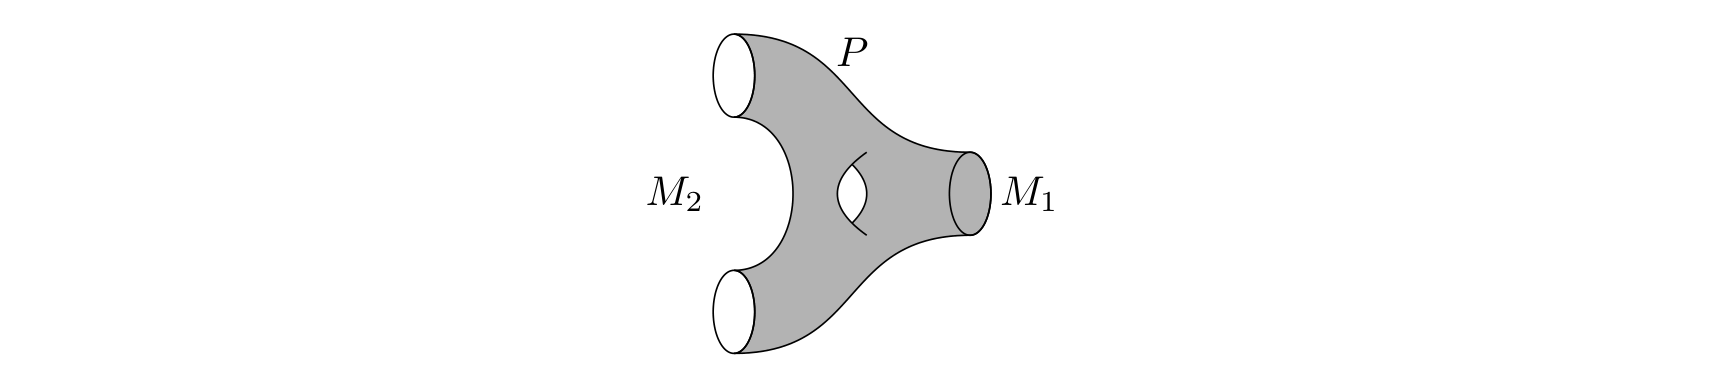
\includegraphics[width=0.58\textwidth]{figure6-1.png}
  \caption{两个对象（闭 $(n-1)$-流形）$M_1$ 与 $M_2$ 之间在 $\Bord_{n-1,n}$ 中的一个态射，
  是以为 $M_1\sqcup M_2$ 边界的 $n$-流形 $P$。（原文 p.~78，Figure 6.1）}
  \label{fig:6-1}
\end{figure}

\begin{figure}[htbp]
  \centering
  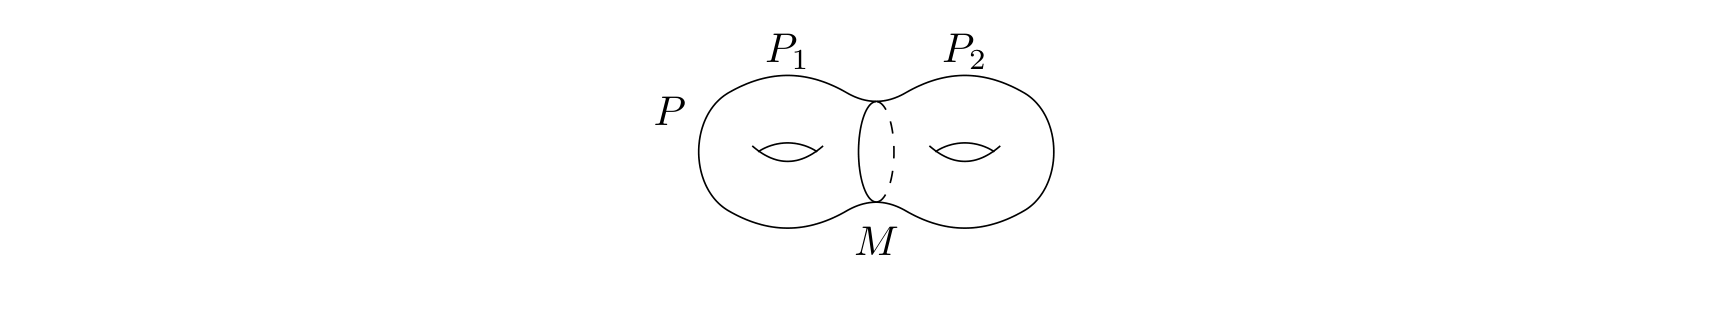
\includegraphics[width=0.55\textwidth]{figure6-2.png}
  \caption{闭 $n$-流形分解为沿 $M$ 相交的两块 $P_1$ 与 $P_2$。（原文 p.~78，Figure 6.2）}
  \label{fig:6-2}
\end{figure}

\subsection{Atiyah--Segal TFT}

一个 Atiyah--Segal（非扩展）TFT 是对称幺半函子
\begin{equation}\tag{6.22}\label{eq:6.22}
\bigl(\Bord_{n-1,n},\sqcup\bigr)\xrightarrow{\ Z\ }\bigl(\Vect,\otimes\bigr).
\end{equation}
$\Bord_{n-1,n}$ 的对象是（定向的\footnote{我们可以要求配边带有不同的切结构；这里只取定向的。}）
闭 $(n-1)$-流形。$\Vect$ 的对象是（复）向量空间。于是闭 $(n-1)$-流形 $M$ 送到某个向量空间 $Z(M)$。
$\Bord_{n-1,n}$ 中的态射 $P\colon M_1\to M_2$ 是一个 $n$-流形 $P$，其边界
$\partial M=M_1\sqcup M_2$，如图 \ref{fig:6-1}。

要理解为什么应该这样想，我们需要把注意力从状态向量空间移开，暂时重新聚焦于闭 $n$-流形 $P$ 上的
配分函数 $Z(P)$。想法是：Atiyah--Segal 对 TFT 的这种形式化，编码了配分函数的局部性。
也就是说，若把 $P$ 切成两块 $P_1$ 与 $P_2$ 并沿 $M$ 粘合（如图 \ref{fig:6-2}），
则 $Z(P)$ 分解为
\diageq{6.23}{0.42\textwidth}{p078_d3.png}

我们更关心 $(n-1)$-流形 $M$ 上的状态向量空间。想法是同样可以把 $Z(M)$ 分解为来自 $M$ 的分解的
“局部块”：
\begin{equation}\tag{6.24}\label{eq:6.24}
M=M_1\sqcup_N M_2,
\end{equation}
其中 $N$ 的余维为 2。我们希望写成
\begin{equation}\tag{6.25}\label{eq:6.25}
Z(M)=\bigl\langle Z(M_1),Z(M_2)\bigr\rangle_{Z(N)},
\end{equation}
但 Atiyah--Segal 形式化没有告诉我们如何做到这一点。这正是扩展场论的基本想法，
它归功于 Freed、Lawrence、Baez--Dolan 等（原文此处只标注了 “cite”，未给出具体文献）。

% [Tutor Note: 式 (6.25) 中的 $\langle-,-\rangle_{Z(N)}$ 是范畴中的 Hom/张量配对（在 2-范畴里即
%  “沿 $Z(N)$ 的态射空间”），不是 Hilbert 空间的内积。若把 $Z(N)$ 想成 $\Shv(\cF(N))$，
%  则这个配对就是层范畴中的 $\otimes_{\Shv(\cF(N))}$ 与 Hom。作者用尖括号是为了提示与
%  向量空间内积的类比，但切勿按内积（共轭线性）理解。]

\begin{figure}[htbp]
  \centering
  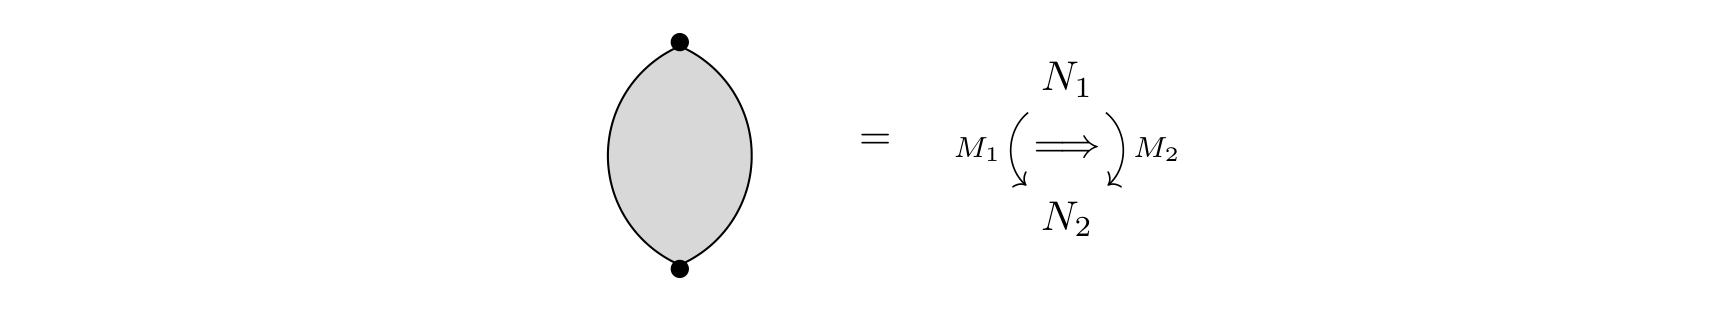
\includegraphics[width=0.6\textwidth]{figure6-3.png}
  \caption{这个带角的流形是 $\Bord_{0,2}$ 中两个 1-态射之间的一个 2-态射。（原文 p.~79，Figure 6.3）}
  \label{fig:6-3}
\end{figure}

基本上，我们需要把某种对象附着到余维 2 的空间。

为形式化这一点，我们定义某种 2-范畴 $\Bord_{n-2,n}$。对象是闭 $(n-2)$-流形 $N$，
态射是以 $N_1\sqcup N_2$ 为边界的 $(n-1)$-流形，2-态射是带角的 $n$-流形。
两个 1-态射之间 2-态射的例子见 $\Bord_{0,2}$ 中的图 \ref{fig:6-3}。

2-层 TFT 是对称幺半函子
\begin{equation}\tag{6.26}\label{eq:6.26}
Z\colon\bigl(\Bord_{n-2,n},\sqcup\bigr)\to\bigl(\cC,\otimes\bigr),
\end{equation}
其中 $(\cC,\otimes)$ 是某个对称幺半 2-范畴。除对称幺半外，我们还希望这个函子如下地还原
“1-层”（即 Atiyah--Segal）形式化。空 $(n-2)$-流形 $\emptyset_{n-2}$ 是 $\Bord_{n-2,n}$ 的单位。
函子是对称幺半的，意味着它被送到单位 $1\in\cC$。空 $(n-2)$-流形的自同态是
\begin{equation}\tag{6.27}\label{eq:6.27}
\End_{\Bord_{n-2,n}}\bigl(\emptyset_{n-2}\bigr)=\Bord_{n,n-1},
\end{equation}
因为空 $\{n-2\}$-流形到自身的配边由闭 $(n-1)$-流形组成。于是我们可能要求 $\cC$ 是 $\Vect$ 的
一个\term{去环路}{delooping}。这只是说
\begin{equation}\tag{6.28}\label{eq:6.28}
\End_{\cC}(1_{\cC})=\Vect .
\end{equation}
此时函子 $Z$ 决定了映射
\begin{equation}\tag{6.29}\label{eq:6.29}
\End_{\Bord_{n-2,n}}\bigl(\emptyset_{n-2}\bigr)=\Bord_{n,n-1}\to\Vect=\End(1_{\cC}).
\end{equation}

无论 $\cC$ 是什么，我们都得到想要的局部性：若 $M=M_1\sqcup_N M_2$，则函子性告诉我们
\begin{equation}\tag{6.30}\label{eq:6.30}
\begin{array}{ccc}
1_{\cC} & \xrightarrow{\ Z(M_1)\ } Z(N) \xrightarrow{\ Z(M_2)\ } & 1_{\cC}\\[6pt]
& \Downarrow{\scriptstyle Z(M)} &
\end{array}
\end{equation}

$\cC$ 的一个自然选择是 $\mathrm{Cat}_{\C}$。其对象是 $\Vect_{\C}$ 上的充实范畴，
1-态射是线性函子，2-态射是线性自然变换。还有别的选择，但这在某种意义下是最基本的一个。
现在我们要把场论延拓到余维 2，以编码分歧。也就是说，我们想要一种方式把余维 2 的 $N$
附着到某个范畴，并（非正式地）把它想成 $\Shv(\cF(N))$。

设 $M$ 是闭 3-流形，$Z$ 是 4 维 TFT，$K\subset M$ 是一个纽结。那么管状纽结的补集 $M_0$ 有边界
$\partial M_0=N$。于是这给出函子
\begin{equation}\tag{6.31}\label{eq:6.31}
Z(N)\xrightarrow{\ Z(M_0)\ } Z(\emptyset)=\Vect .
\end{equation}

% [Tutor Note: 式 (6.27)--(6.29) 是“去环路”条件的标准表述，但 2-范畴 $\cC$ 的环路
%  $\End_\cC(1_\cC)$ 只在 $\cC$ 是单对象 2-范畴（即带 $E_1$ 结构的幺半范畴）时才是通常意义的
%  幺半范畴。此处作者取 $n=2$ 的例子（$\Bord_{0,2}$）作直观；对一般的 $n$，$\Bord_{n-2,n}$
%  是 $n$-范畴，去环路需迭代。严格的完全扩展 TFT 由配边假设（cobordism hypothesis，
%  Lurie）刻画：$Z$ 由 $Z(\mathrm{pt})$ 作为可对偶对象唯一决定。建议对照 [Lur09] 第 2.3 节。]

想法是：我们从某个向量空间 $Z(M)$ 出发，沿边界按某个条件修改它，得到向量空间 $Z(M_0)$。

我们去掉的东西的内部，即纽结的环面邻域，记作 $M_1$，它定义了函子 $\Vect\to Z(N)$；
函子性给出
\begin{equation}\tag{6.32}\label{eq:6.32}
\begin{array}{ccc}
\Vect & \xrightarrow{\ Z(M_1)\ } Z(N) \xrightarrow{\ Z(M_0)\ } & \Vect\\[6pt]
& \Downarrow{\scriptstyle Z(M)} &
\end{array}
\end{equation}
这就是扩展场论编码我们一直讨论的边界条件的方式。

\section{阿贝尔对偶的例子}

\begin{sectionkey}
本节把第 3 章的两个二维阿贝尔对偶例子放到余维 2 的分歧下重新审视：A-侧的场空间由同伦型决定，
B-侧必须取栈（而不能只取同构类），于是“点”上的范畴一边是分次向量空间、另一边是 $\C^\times$ 的表示；
这两者由 Fourier 对偶（Pontrjagin 对偶的范畴化）等同。
\end{sectionkey}

回忆第 3 章的阿贝尔对偶。特别是第 3.7.2 节、第 3.7.3 节与第 4.6 节中的二维例子。
现在我们在这些例子中加入余维 2 的分歧来讨论。

\subsection{二维情形}

回忆第一个例子把 A-侧的 $H^0(S^1,\Z)$ 与 B-侧的 $H^1(S^1,\C^{\times})$ 交换。
在 A-侧，场由
\begin{equation}\tag{6.33}\label{eq:6.33}
\cF(-)=\operatorname{Maps}(-,\Z)
\end{equation}
给出，故在连通流形上场看起来就是 $\Z$。唯一余维为 2 的子流形是点，而附着到点的范畴是
\begin{equation}\tag{6.34}\label{eq:6.34}
Z(\mathrm{pt})=\Shv(\Z)=\Vect^{\Z\text{-gr}},
\end{equation}
即分次向量空间的范畴。

在 B-侧，我们把 $H^1(S^1,\C^{\times})$ 解释为 $S^1$ 上 $\C^{\times}$-局部系统的同构类。
这建议我们的场空间应该是
\begin{equation}\tag{6.35}\label{eq:6.35}
\cF(-)=\Loc_{\C^{\times}}(-).
\end{equation}
若真的只考虑同构类构成的集合，我们不会得到附着到点的范畴：$\Loc_{\C^{\times}}(\mathrm{pt})$
只是单点，故与另一侧不匹配。相反，我们必须把它想成一个栈。它仍然是点，
但带 $\C^{\times}$ 通过自同构的作用。也就是说，它是栈
\begin{equation}\tag{6.36}\label{eq:6.36}
B\C^{\times}=\mathrm{pt}/\C^{\times}.
\end{equation}
取层时得到
\begin{equation}\tag{6.37}\label{eq:6.37}
\Shv\bigl(\cF(\mathrm{pt})\bigr)=\Shv\bigl(\mathrm{pt}/\C^{\times}\bigr)
=\Rep\bigl(\C^{\times}\bigr)\simeq\Vect^{\Z\text{-gr}}.
\end{equation}
$\C^{\times}$ 的表示与分次向量空间之间的等同如下给出。给定 $\C^{\times}$ 的表示 $V$，得到分次
\begin{equation}\tag{6.38}\label{eq:6.38}
V=\bigoplus_{n\in\Z}V_n,
\end{equation}
其中 $V_n$ 是 $z\in\C^{\times}$ 以 $z^n$ 作用的部分。

% [Tutor Note: (6.36)--(6.37) 是本章的关键机制，也是初学者最容易出错的地方：
%  $\Loc_{\C^\times}(\mathrm{pt})$ 作为集合只是一个点，但作为栈它是 $B\C^\times=\mathrm{pt}/\C^\times$，
%  其上的拟凝聚层/局部系统给出 $\Rep(\C^\times)\simeq\Vect^{\Z\text{-gr}}$。
%  若在 A-侧同样只取同构类，就丢掉了 $\Z$-分次结构，两边不可能等同。
%  另外需注意：$\Shv(\Z)$ 这里指 $\Z$（离散群）上局部系统的范畴，等价于分次向量空间，
%  而不是 $\Z$ 上层的导出范畴。]

我们可以如下把它看成 Pontrjagin 对偶的某种版本。可以把 $\Shv(\Z)$ 想成带逐点乘法的
$\C[\Z]$ 的模：
\begin{equation}\tag{6.39}\label{eq:6.39}
\Shv(\Z)=(\C[\Z],\cdot)\text{-mod}.
\end{equation}
对偶地，$\C^{\times}$ 的表示可以想成带卷积的 $\C[\C^{\times}]$ 的模：
\begin{equation}\tag{6.40}\label{eq:6.40}
\Rep\bigl(\C^{\times}\bigr)=(\C\C^{\times},*)\text{-mod}.
\end{equation}
这一对偶断言这两个范畴等价。在 B-侧我们真正看的是 $\C^{\times}$ 上代数函数的余模，
即 $\C[\C^{\times}]$-comod；也就是说，$\Z$ 上函数的模是 $\C^{\times}$ 上函数的余模。

\subsection{二维情形}

回忆第 3.7.3 节与第 4.6 节，那里讨论了二维阿贝尔对偶的另一个例子。A-侧由 $H^1(S^1,\Z)$ 上的
函数给出，B-侧由 $H^0(S^1,\C^{\times})$ 上的函数给出。这是 T-对偶或镜像对称的基本例子。

在 A-侧，我们可以把它想成
\begin{equation}\tag{6.41}\label{eq:6.41}
H^1(S^1,\Z)=H^0(S^1,B\Z).
\end{equation}
这建议场空间由
\begin{equation}\tag{6.42}\label{eq:6.42}
\cF(-)=\operatorname{Maps}\bigl(-,B\Z=S^1\bigr)
\end{equation}
给出，故
\begin{equation}\tag{6.43}\label{eq:6.43}
\cF(\mathrm{pt})=S^1=B\Z .
\end{equation}
于是所要的范畴是它上面的某种层，我们取为局部常值的：
\begin{equation}\tag{6.44}\label{eq:6.44}
\Shv(B\Z):=\Loc(S^1)=\Rep(\Z)=(\C\Z,*)\text{-mod}.
\end{equation}
这个范畴的另一个名字是 $T^*S^1$ 的（卷绕）Fukaya 范畴。要点是：$T^*S^1$ 的辛拓扑就是
$S^1$ 的普通拓扑。

在 B-侧，圆周上的场由 $H^0(S^1,\C^{\times})$ 给出，这告诉我们场是到带离散拓扑的 $\C^{\times}$ 的映射：
\begin{equation}\tag{6.45}\label{eq:6.45}
\cF(-)=\operatorname{Maps}\bigl(-,\C^{\times}_{\mathrm{disc}}\bigr).
\end{equation}
特别地，
\begin{equation}\tag{6.46}\label{eq:6.46}
\cF(\mathrm{pt})=\C^{\times},
\end{equation}
而自然的层范畴将是拟凝聚的\footnote{这与 A-侧我们所用的局部常值层形成对比。}：
\begin{equation}\tag{6.47}\label{eq:6.47}
\Shv_B\bigl(\C^{\times}\bigr):=\QC\bigl(\C^{\times}\bigr)
=(\C[\C^{\times}],\cdot)\text{-mod}
=\C[z,z^{-1}]\text{-mod}.
\end{equation}

% [Tutor Note: 原文第 6.3 节的两个子节标题都写作 “Two-dimensions”，这是作者的重复，
%  并非排版偶然（源文 p.79 与 p.80 均如此）。这里按原文照译，便于对照；
%  内容上两小节分别处理 $H^0\leftrightarrow H^1$ 与 $H^1\leftrightarrow H^0$ 两组对偶。]

再次看到，这在模仿我们在 Pontrjagin 对偶情形所见。在 A-侧我们有带卷积的 $\C[\Z]$ 的模，
在 B-侧我们有带逐点乘法的 $\C[\C^{\times}]$ 的模。

换言之，可以把 $\C[z,z^{-1}]$ 想成 $\C^{\times}$ 上的函数，或想成 $\Z$ 的群代数 $\C[\Z]$：
\begin{equation}\tag{6.48}\label{eq:6.48}
\text{$\C^{\times}$ 上的函数}=\C[z,z^{-1}]=\C[\Z],
\end{equation}
故一个模既可以看作圆周上的局部系统，也可以看作 $\C^{\times}$ 上的层。

这是同调镜像对称的第一个例子：
\begin{equation}\tag{6.49}\label{eq:6.49}
\operatorname{Fuk}^{wr}\bigl(T^*S^1\bigr)=\Loc(S^1)\simeq\QC\bigl(\C^{\times}\bigr).
\end{equation}

\section{四维 Maxwell 理论}

\begin{sectionkey}
本节把四维拓扑 Maxwell 理论的对偶降到余维 2（曲面）：A-侧的 $\operatorname{Pic}\Sigma$
与 B-侧的 $\C^\times$-局部系统 $\Loc_{\C^\times}(\Sigma)$ 上的层范畴，经由 Fourier--Mukai 变换等同；
这也给出 $G=\mathrm{GL}_1$ 的 Betti 几何 Langlands 对应的一个初等例子。
\end{sectionkey}

回忆第 4.8.1 节的四维 Maxwell 理论。这个对偶把 A-侧线丛的拓扑与 B-侧平坦线丛的代数几何交换。
回忆这个对偶把 A-侧的 $H^2(M^3,\Z)$ 与 B-侧的 $H^1(M^3,\C^{\times})$ 交换。
现在我们要把第 4.5.1 节中余维 1 的缺陷降到余维 2，即降到曲面。

\subsection{A-侧}

设 $\Sigma$ 是曲面。在 A-侧我们有
\begin{equation}\tag{6.50}\label{eq:6.50}
H^2(-,\Z)=\pi_0\Bigl(\operatorname{Map}\bigl(-,\underbrace{BU(1)}_{K(\Z,2)}\bigr)\Bigr),
\end{equation}
即我们在探测某个更大对象的连通分量。这建议我们的场应该类似
\begin{equation}\tag{6.51}\label{eq:6.51}
\cF(-)=\operatorname{Map}\bigl(-,BU(1)\bigr).
\end{equation}
我们把这些记作 $\operatorname{Pic}\Sigma$：
\begin{equation}\tag{6.52}\label{eq:6.52}
\cF(\Sigma)=\operatorname{Pic}\Sigma:=\operatorname{Map}\bigl(\Sigma,BU(1)\bigr).
\end{equation}
为更清楚地看出与线丛的等同，在 $\Sigma$ 上取一个复结构（于是它现在是 Riemann 面）。
然后可以看 $\Sigma$ 上全纯/代数线丛构成的空间 $\operatorname{Pic}\Sigma$。这是代数几何的对象，
但我们只关心其拓扑。故此空间不依赖复结构，但选一个复结构让我们能显式地实现这个空间。
它适合短正合列
\begin{equation}\tag{6.53}\label{eq:6.53}
0\to\operatorname{Jac}\Sigma\to\operatorname{Pic}\Sigma\xrightarrow{\ \deg\ }\Z\to 0,
\end{equation}
其中 $\operatorname{Jac}\Sigma$ 由 0 次线丛组成。断言是 $\operatorname{Jac}\Sigma$ 是实维 $2g$ 的环面，
故拓扑上它就是
\begin{equation}\tag{6.54}\label{eq:6.54}
\operatorname{Jac}\Sigma\simeq \C^g/\Z^{2g}.
\end{equation}

\begin{srcrem}{27}
我们又一次忽略了这些线丛的自同构，它们会贡献额外的（栈性）因子 $BU(1)$。
\end{srcrem}

我们如下得到显式描述。指数短正合列
\begin{equation}\tag{6.55}\label{eq:6.55}
0\to\Z\to\cO\to\cO^{\times}\to 0
\end{equation}
给出
\begin{equation}\tag{6.56}\label{eq:6.56}
0\to H^1(\Sigma,\cO)/H^1(\Sigma,\Z)\to H^1(\Sigma,\cO^{\times})
\to H^2(\Sigma,\Z)=\Z\to 0,
\end{equation}
故
\begin{equation}\tag{6.57}\label{eq:6.57}
\operatorname{Jac}\simeq K\bigl(H^1(\Sigma,\Z),1\bigr),
\end{equation}
即以 $H^1(\Sigma,\Z)$ 为 $\pi_1$ 的环面。

因此，这个阿贝尔范畴可以写成
\begin{align}
\Loc(\operatorname{Pic}\Sigma)
&=\Vect^{\Z\text{-gr}}\otimes\Loc(\operatorname{Jac}\Sigma)\tag{6.58}\label{eq:6.58}\\
&=\Rep_{\Z\text{-gr}}\bigl(\Lambda=H^1(\Sigma,\Z)\bigr)\tag{6.59}\label{eq:6.59}\\
&=\Vect^{\Z\text{-gr}}\otimes\bigl(\C[H^1(\Sigma,\Z)],*\bigr).\tag{6.60}\label{eq:6.60}
\end{align}

\begin{flushright}
\small 第 12 讲；2021 年 3 月 4 日
\end{flushright}

\subsection{B-侧}

现在我们来检查在 B-侧该做什么，那里我们研究 $\C^{\times}$-局部系统的代数几何。
也就是说，对曲面 $\Sigma$（不必带复结构），我们考虑
\begin{align}
\Loc_{\C^{\times}}(\Sigma)
&=\Hom\bigl(\pi_1(\Sigma),\C^{\times}\bigr)/\C^{\times}\tag{6.61}\label{eq:6.61}\\
&=\Hom\bigl(H_1(\Sigma,\Z),\C^{\times}\bigr)/\C^{\times}\tag{6.62}\label{eq:6.62}\\
&\simeq\bigl(H^1(\Sigma,\Z)\otimes_{\Z}\C^{\times}\bigr)/\C^{\times}.\tag{6.63}\label{eq:6.63}
\end{align}
现在应该附着某种（层）范畴。我们在做代数几何，故自然的层范畴是
\begin{equation}\tag{6.64}\label{eq:6.64}
\QC\bigl(\Loc_{\C^{\times}}\Sigma\bigr)
=\bigl(\C[\Loc_{\C^{\times}}(\Sigma)],\cdot\bigr)\text{-mod}
\otimes\Rep\bigl(\C^{\times}\bigr).
\end{equation}
这个函数环可以写成
\begin{equation}\tag{6.65}\label{eq:6.65}
\C\bigl[\Loc_{\C^{\times}}(\Sigma)\bigr]=\C\bigl[H^1(\Sigma,\Z)\bigr].
\end{equation}
现在由 Poincaré 对偶有 $H^1(\Sigma,\Z)\simeq H_1(\Sigma,\Z)$。又已见
$\Rep\C^{\times}=\Vect^{\Z\text{-gr}}$。

现在可以把这与 A-侧式 \eqref{eq:6.60} 比较。带卷积的格代数 $(\C\Lambda,*)$ 通过 Fourier 级数
与 $(\C[T^{\vee}],\cdot)$ 等同。这意味着这两个代数上的模相同，即
\begin{equation}\tag{6.66}\label{eq:6.66}
\Loc K(\Lambda,1)\simeq\QC\bigl(T^{\vee}_{\C}\bigr).
\end{equation}
这里左端是 $\Loc\operatorname{Jac}(\Sigma)$，右端是 $\QC(\Loc)$ 但忽略了 $\C^{\times}$ 的额外作用。

于是结论是
\begin{equation}\tag{6.67}\label{eq:6.67}
\Loc\operatorname{Pic}(\Sigma)\simeq\QC(\Loc).
\end{equation}
这就是我们对余维 2 的拓扑 Maxwell 理论的阿贝尔对偶。

\begin{srcrem}{28}
这是 Fourier--Mukai 变换的第一个例子，即层范畴的 Fourier 变换版本。
\end{srcrem}

\begin{srcrem}{29}
这是 $G=\mathrm{GL}_1$ 的 Betti 几何\footnote{“几何”只是指我们在范畴层面看问题。}
Langlands 对应的陈述。
\end{srcrem}

% [Tutor Note: 式 (6.56) 的长正合列容易看漏一处：$H^1(\Sigma,\cO)/H^1(\Sigma,\Z)$ 中的
%  $H^1(\Sigma,\Z)$ 通过指数正合列嵌入 $H^1(\Sigma,\cO)$，这一步用的是 $H^2(\Sigma,\Z)=\Z$
%  与 $H^2(\Sigma,\cO)=0$（对紧 Riemann 面）。于是 $\operatorname{Jac}\simeq K(H^1(\Sigma,\Z),1)$，
%  其复结构来自 $H^1(\Sigma,\cO)/H^1(\Sigma,\Z)$。另注意 (6.66) 中对偶环面 $T^{\vee}_{\C}$ 的
%  下标是复数域：这里的“Fourier 对偶”是在复环面层面，$\pi_1$ 与 $H^1$ 互换。]

\subsection{带分歧的电磁对偶}

我们想写出带分歧的一般电磁对偶。这将包括 Dirac 单极子（第 4.5.1 节）与螺线管（第 4.8.2 节）。
回忆曲面 $\Sigma$ 作为 3-流形 $M_0=M\setminus K$ 的边界出现，其中 $K\subset M$ 是一个纽结。

在 A-侧，我们有（限制）映射
\begin{equation}\tag{6.68}\label{eq:6.68}
\operatorname{Pic}(M_0)\xrightarrow{\ \pi\ }\operatorname{Pic}(\Sigma),
\end{equation}
这里我们仍只从拓扑上考虑 $\operatorname{Pic}$。设 $\cE\in\Loc(\operatorname{Pic}\Sigma)$。
则得到
\begin{equation}\tag{6.69}\label{eq:6.69}
\pi^*\cE\in\Loc\bigl(\operatorname{Pic}(M_0)\bigr),
\end{equation}
并且可以附着如下向量空间：
\begin{equation}\tag{6.70}\label{eq:6.70}
\Gamma\bigl(\operatorname{Pic}(M_0),\pi^*\cE\bigr).
\end{equation}
这是我们说“用某些分歧数据修改 $Z(M)$”的方式。

在 B-侧，我们也可以限制
\begin{equation}\tag{6.71}\label{eq:6.71}
\Loc_{\C^{\times}}M_0\xrightarrow{\ \pi^{\vee}\ }\Loc_{\C^{\times}}\Sigma,
\end{equation}
然后可以把 $\cE^{\vee}\in\QC(\Loc_{\C^{\times}}\Sigma)$ 拉回，得到
\begin{equation}\tag{6.72}\label{eq:6.72}
\pi^{\vee*}\cE^{\vee}\in\QC\bigl(\Loc_{\C^{\times}}M_0\bigr),
\end{equation}
并且可以附着如下向量空间：
\begin{equation}\tag{6.73}\label{eq:6.73}
\Gamma\bigl(M_0,\pi^{\vee*}\cE^{\vee}\bigr).
\end{equation}
于是带分歧的电磁对偶通过 Fourier--Mukai 变换交换 $\cE$ 与 $\cE^{\vee}$。特别地，它告诉我们
\begin{equation}\tag{6.74}\label{eq:6.74}
\Gamma\bigl(\operatorname{Pic}M_0^3,\pi^*\cE\bigr)
\simeq\Gamma\bigl(\Loc_{\C^{\times}}M,\pi^{\vee*}\cE^{\vee}\bigr).
\end{equation}
层 $\cE$ 与 $\cE^{\vee}$ 规定边界条件，例如 Dirichlet 或 Neumann。例如 $\cE^{\vee}$ 可能是
$\Loc_{\C^{\times}}(\Sigma)$ 中某个轨迹的结构层。于是我们看的是沿该轨迹带有特定奇点的局部系统，
即 $\Loc M_0$ 中那些限制到边界 $\Sigma$ 后落到特定子集的元素。

% [Tutor Note: 式 (6.74) 的记号与上下文不完全一致：左端的 $M_0^3$ 应即三维流形 $M_0$（上标 $3$
%  表示维数），右端的 $\Loc_{\C^{\times}}M$ 按限制映射 (6.71) 的源应为 $\Loc_{\C^{\times}}M_0$
%  （去掉纽结后的流形），而不是整个 $M$。作者混用了 $M$ 与 $M_0$。理解时以 (6.73) 为准：
%  两边分别是 $\Gamma(\operatorname{Pic}(M_0),\pi^*\cE)$ 与 $\Gamma(M_0,\pi^{\vee*}\cE^{\vee})$。]

\section{带分歧的类域论}

\begin{sectionkey}
本节把 3-流形/纽结的拓扑图景平移到曲线 $C/\F_q$ 与其上一点 $x$：$K_x^\times$ 的作用代替了
边界层的拉回，局部类域论给出 $K_x^\times$ 的表示与 $D_x^\times$ 上秩 1 局部系统（即
$\Gal(\overline{K}_x/K_x)$ 的特征）的对偶，而整体类域论把 $\operatorname{Pic}$ 的“带水平结构版本”
与在 $S$ 处分歧的 Galois 特征对应起来。
\end{sectionkey}

设 $C/\F_q$ 是有限域上的曲线。对点 $x\in C$，我们想在这一点“允许分歧”。
考虑分歧曲线内 $x$ 周围的穿孔圆盘：
\begin{equation}\tag{6.75}\label{eq:6.75}
\Spec K_x=D_x^{\times}\hookrightarrow C\setminus x .
\end{equation}
注意 $K_x\simeq \F_q((t))$。这幅图是“管状邻域的边界位于 3-流形内部”的类比：
\begin{equation}\tag{6.76}\label{eq:6.76}
N=\partial\bigl(\text{$K$ 的管状邻域}\bigr)\hookrightarrow M_0=M\setminus K .
\end{equation}
所以现在切除的是点（而不是纽结），并且我们要理解的是这个穿孔圆盘，
而不是纽结管状邻域的边界。

在 B/Galois 侧，我们看的是 $\Loc_1(C\setminus x)$。无论这些是什么，它们都可以限制到穿孔圆盘：
\begin{align}
\Loc_1(C\setminus x)\to\Loc_1 D^{\times}
&=\Hom_{cts}\bigl(\Gal(\overline{K}_x/K_x),\overline{\Q}_{\ell}^{\times}\bigr)\tag{6.77}\label{eq:6.77}\\
&=\Hom_{cts}\bigl(\Gal^{ab}(\overline{K}_x/K_x),\overline{\Q}_{\ell}^{\times}\bigr).\tag{6.78}\label{eq:6.78}
\end{align}
也就是说，我们研究的是 Abel 化 Galois 群的特征，但它们作为 $D^{\times}$ 上的局部系统出现。
于是现在的想法是：研究 $C\setminus x$ 上带有绕该穿孔点的特定分歧数据的局部系统。

在 A-侧，我们看的是 $\operatorname{Pic}C$。回忆第 5.2.2 节中它的阿黛尔描述：
\begin{align}
\operatorname{Pic}C
&=F^{\times}\Big\backslash\sideset{}{'}\prod_{y\in C}K_y^{\times}
\Big/\prod_{y\in C}\cO_y^{\times}\tag{6.79}\label{eq:6.79}\\
&=F^{\times}\Big\backslash\sideset{}{'}\prod\Z .\tag{6.80}\label{eq:6.80}
\end{align}
对穿孔曲线有类似的描述：
\begin{equation}\tag{6.81}\label{eq:6.81}
\operatorname{Pic}(C\setminus x)
=F^{\times}\Big\backslash\sideset{}{'}\prod_{y\in C\setminus x}K_y^{\times}
\Big/\prod_{y\in C\setminus x}\cO_y^{\times}.
\end{equation}
我们可以把它写成
\begin{align}
\operatorname{Pic}(C\setminus x)
&=F^{\times}\Big\backslash\sideset{}{'}\prod_{y\in C\setminus x}K_y^{\times}
\Big/\prod_{y\in C\setminus x}\cO_y^{\times}\tag{6.82}\label{eq:6.82}\\
&=\operatorname{Pic}C\Big/\bigl(\Z_x=K_x^{\times}/\cO_x^{\times}\bigr),\tag{6.83}\label{eq:6.83}
\end{align}
这里我们模掉的是“加减这个点 $x$ 的拷贝”。然后也可以把它写成
\begin{align}
\operatorname{Pic}(C\setminus x)
&=F^{\times}\Big\backslash\sideset{}{'}\prod_{y\in C\setminus x}K_y^{\times}
\Big/\prod_{y\in C\setminus x}\cO_y^{\times}\tag{6.84}\label{eq:6.84}\\
&=\operatorname{Pic}C\Big/\bigl(\Z_x=K_x^{\times}/\cO_x^{\times}\bigr)\tag{6.85}\label{eq:6.85}\\
&=\operatorname{Pic}(C,\widehat{x})\big/K_x^{\times},\tag{6.86}\label{eq:6.86}
\end{align}
其中 $\operatorname{Pic}(C,\widehat{x})$ 定义为 $C$ 上配备 $D_x$ 上平凡化的线丛。
故我们在右边模掉这个平凡化。

$\operatorname{Pic}(C,\widehat{x})$ 映到 $\operatorname{Pic}C$，其纤维由平凡化的改变给出，
并有中间对象 $\operatorname{Pic}(C,nx)$（$n\in\Z^{+}$）：
\begin{equation}\tag{6.87}\label{eq:6.87}
\begin{array}{ccc}
\operatorname{Pic}(C,\widehat{x}) & \xrightarrow{\ \cO_x^{\times}\ } & \operatorname{Pic}(C)\\[2pt]
\searrow & & \nearrow\\[2pt]
& \operatorname{Pic}(C,nx) &
\end{array}
\end{equation}
其中 $\operatorname{Pic}(C,nx)$ 由 $\operatorname{Pic}(C)$ 中在 $x$ 周围有 $n$ 阶平凡化的对象组成。
这个说法告诉我们：要研究穿孔曲线，并不需要真的穿孔。只要理解 $K_x^{\times}$ 如何作用，
就可以研究 $C$ 上配备平凡化的丛。

% [Tutor Note: 原文 (6.81)--(6.86) 有重复排版：式 (6.81) 与 (6.82) 的左端表达式相同，
%  (6.84) 与 (6.82)、(6.85) 与 (6.83) 分别重复（源文 p.84--85）。这里照原文保留，
%  只为便于对照；逻辑上只需 (6.81)--(6.83) 与 (6.86)。另外 (6.79) 中的 $\prod'$ 表示
%  限制直积：除有限多个因子外，$K_y^{\times}$ 的因子都落在 $\cO_y^{\times}$ 中。]

无论如何，$\operatorname{Pic}(C,\widehat{x})$ 上有 $K_x^{\times}$ 的作用。所以我们将看
$\operatorname{Pic}(C,\widehat{x})$ 上的函数，并在这个作用下分解它们。从 TFT 的观点，
我们说得略有不同。也就是说，我们有限制
\begin{equation}\tag{6.88}\label{eq:6.88}
\begin{array}{ccc}
\operatorname{Pic}(C\setminus x) & = & \operatorname{Pic}(C,\widehat{x})/K^{\times}\\[2pt]
\downarrow & & \downarrow\\[2pt]
\operatorname{Pic}(D_x^{\times}) & = & \mathrm{pt}/K^{\times},
\end{array}
\end{equation}
并且可以取一个层并在 $\operatorname{Pic}(C,\widehat{x})$ 上取整体截面，即前推到 $\mathrm{pt}/K_x^{\times}$。
研究这幅图等价于研究 $K^{\times}$ 在 $\operatorname{Pic}(C,\widehat{x})$ 上的作用。

数论学家会告诉你，你不想要“无限水平结构”。我们有 $K=\F_q((t))$。于是
\begin{equation}\tag{6.89}\label{eq:6.89}
K^{\times}=\F_q((t))^{\times}\supset\cO^{\times}=\F_q[[t]].
\end{equation}
它还包含这些子群：
\begin{equation}\tag{6.90}\label{eq:6.90}
K^{\times}\supset\cO^{\times}\supset\cO^{\times(1)}\supset\cdots\supset\cO^{\times(n)}\supset\cdots
\end{equation}
其中属于 $\cO^{\times(n)}$ 只意味着你形如 $(1+t^n)(-)$。

之前，商 $K^{\times}/\cO^{\times}=\Z$ 给我们除子。故在非分歧情形，我们有 $\Z$ 作用在
$\operatorname{Pic}(C)$ 上。现在当我们添加水平结构，即从 $\operatorname{Pic}(C)$ 过渡到
$\operatorname{Pic}(C,nx)$ 时，我们有 $K^{\times}/\cO^{\times(n)}$ 的作用。

所以我们做的是看 $K^{\times}$ 的\term{光滑表示}{smooth representation}，即每个向量都被某个
$\cO^{\times(N)}$（$N\gg 0$）固定。若给它作用的那个东西以离散拓扑，这等价于拓扑连续性。

现在要建立如下图景的类比：对以 $\partial M_0=\Sigma$ 为边界的 3-流形 $M_0$，我们得到
\begin{equation}\tag{6.91}\label{eq:6.91}
Z(M_0)\in Z(\Sigma).
\end{equation}
这里的类比如下。对 $C/\F_q$ 与 $x\in C$，我们可以附着
\begin{equation}\tag{6.92}\label{eq:6.92}
\operatorname{Pic}(C,\widehat{x}).
\end{equation}
现在我们要考虑
\begin{equation}\tag{6.93}\label{eq:6.93}
\C\bigl[\operatorname{Pic}(C,\widehat{x})\bigr],
\end{equation}
具体地把它想成 $K_x^{\times}$ 的表示。这可以看作取常值层 $k_{\operatorname{Pic}(C\setminus x)}$
并前推，得到
\begin{equation}\tag{6.94}\label{eq:6.94}
\pi_*k\in\Shv\bigl(\mathrm{pt}/K^{\times}\bigr)=\operatorname{Pic}\bigl(D^{\times}\bigr),
\end{equation}
即 $K^{\times}$ 的一个表示。

于是在 A-侧，我们有来自带无限水平结构的 $\operatorname{Pic}$（即 $\operatorname{Pic}(C,\widehat{x})$，
或某个有限水平结构 $\operatorname{Pic}(C,nx)$）的 $K^{\times}$ 表示。

在 B-侧，我们有层 $\cO_{\Loc(C\setminus x)}$，把它前推得到 $\Loc_1(D^{\times})$ 上的层，
即 $D^{\times}$ 上函数的模。现在我们需要注 28 中 Fourier--Mukai 变换的类比。

这正是局部类域论的内容。

整体类域论说
\begin{equation}\tag{6.95}\label{eq:6.95}
\Gal^{ab,ur}\simeq\widehat{\operatorname{Pic}},
\end{equation}
其中 $\widehat{\operatorname{Pic}}$ 表示 profinite 完备化。局部类域论的陈述是：存在典范映射
\begin{equation}\tag{6.96}\label{eq:6.96}
K_x^{\times}\to\Gal^{ab}\bigl(\overline{K}_x/K_x\bigr),
\end{equation}
它在 profinite 完备化之后是同构：
\begin{equation}\tag{6.97}\label{eq:6.97}
\widehat{K_x^{\times}}\xrightarrow{\ \sim\ }\Gal^{ab}\bigl(\overline{K}_x/K_x\bigr).
\end{equation}
这告诉我们，$K^{\times}$ 的群环与如下对象 Pontrjagin 对偶：
\begin{equation}\tag{6.98}\label{eq:6.98}
\Hom\bigl(\Gal^{ab}(\overline{K}_x/K_x),\overline{\Q}_{\ell}^{\times}\bigr)
=\Hom\bigl(\Gal(\overline{K}_x/K_x),\overline{\Q}_{\ell}^{\times}\bigr)
=\Loc_1(C).
\end{equation}
换言之，
\begin{equation}\tag{6.99}\label{eq:6.99}
\bigl(\overline{\Q}_{\ell}^{\times}[K^{\times}],*\bigr)
\simeq\bigl(\overline{\Q}_{\ell}^{\times}[\Loc_1],\cdot\bigr).
\end{equation}
这类似于在 Riemann 面情形我们把 $\pi_1\operatorname{Jac}=\Lambda$ 与 $\C[T^{\vee}]$ 交换。
现在过渡到模，得到
\begin{equation}\tag{6.100}\label{eq:6.100}
\Rep\bigl(K^{\times}\bigr)=\QC(\Loc_1 C).
\end{equation}
要把这样的陈述在技术上精确化需要大量工作。故局部陈述是：穿孔圆盘上的局部系统与
$K^{\times}$ 的表示有关。而整体陈述是：附着到穿孔曲面的向量空间，即 $K^{\times}$ 的表示，
等同于带有指定分歧的局部系统。

% [Tutor Note: 式 (6.98) 末项在原文中写作 $\Loc_1(C)$（源文 p.86）。按上下文，这里应是
%  $K_x$ 的局部域对应，即 $D_x^{\times}$（或 $C\setminus x$）上秩 1 局部系统的范畴
%  $\Loc_1(D_x^{\times})=\Loc_1(C\setminus x)$，而不是整条曲线 $C$ 上的 $\Loc_1(C)$。
%  这可能是作者把 $C$ 与 $C\setminus x$（或 $D^\times$）混写；同类混写在 (6.74) 中也出现过。
%  另外 (6.95) 的 $\Gal^{ab,ur}$ 是整体类域论中的“非分歧 Abel 化 Galois 群”，
%  而 (6.96)--(6.97) 是局部对应，二者不可混用。]

\section{数域的分歧}

\begin{sectionkey}
本节把上一节的函数域图景逐字搬到数域：局部类域论给出 $K_v^{\times}$ 到局部 Abel 化 Galois 群的
典范映射（在 profinite 完备化后为同构），整体类域论则把带 $S$ 外非分歧条件的阿黛尔商与
在 $S$ 处分歧的 Galois 特征对应起来。
\end{sectionkey}

对数域，陈述非常相似。局部类域论说：对 $F$ 的非 Archimedes 位 $v$，即 $\cO_F$ 中的一个素元，
存在自然映射
\begin{equation}\tag{6.101}\label{eq:6.101}
K_v^{\times}\to\Gal^{ab}\bigl(\overline{K}/K\bigr),
\end{equation}
它在 profinite 完备化上是同构：
\begin{equation}\tag{6.102}\label{eq:6.102}
\widehat{K_v^{\times}}\xrightarrow{\ \sim\ }\Gal^{ab}\bigl(\overline{K}/K\bigr).
\end{equation}
我们可以把这理解为：把 $K^{\times}$ 的表示与 $\mathrm{GL}_1$ 上的函数模、以及 Galois 表示
等同起来（例如取 $K_v=\Q_p$）。

整体类域论说如下。$\operatorname{Pic}(C,\widehat{x})$ 的类比是
\begin{equation}\tag{6.103}\label{eq:6.103}
F^{\times}\Big\backslash\prod_v K^{\times}\Big/\prod_{v\notin S}\cO^{\times},
\end{equation}
而这个东西上的函数带有
\begin{equation}\tag{6.104}\label{eq:6.104}
\prod_{v\in S}K_v^{\times}
\end{equation}
的作用。故我们可以在这个作用下分解它们。这将与在 $S$ 处分歧的 Galois 群的特征（上的函数）相匹配。

% [Tutor Note: 原文 (6.103)--(6.104) 中 $S$ 的含意需要小心：$S$ 是“允许分歧”的有限位集，
%  故在 $S$ 外取整（$\prod_{v\notin S}\cO^{\times}$），而作用来自 $S$ 内的 $K_v^{\times}$。
%  注意 (6.103) 中 $\prod_v$ 的上标 $'$（限制直积）在原文 p.87 被省略，严格写法应为
%  $F^{\times}\backslash\prod'_v K^{\times}/\prod_{v\notin S}\cO^{\times}$。
%  此外 p.87 的原文把 “E.g.\ think $K_v=\Q_p$” 插在句子中间，导致 “representations of
%  $K^\times$ with modules for functions on $\mathrm{GL}_1$ Galois representations” 一句
%  语序破碎；这里按数学含义译出，但源文的断句确实可疑。]

\begin{flushright}
\small 第 13 讲；2021 年 3 月 9 日
\end{flushright}

% ============================================================================
%  第 7 章  几何类域论
% ============================================================================
\chapter{几何类域论}\label{ch:07}

\begin{keytakeaways}
本章讨论几何类域论（即函数域上的类域论）的几何形式。核心论点是：
$\operatorname{Pic}$ 上带有“乘性”性质的秩 1 局部系统（特征局部系统/特征层），
与曲线 $C$ 上的秩 1 局部系统一一对应；其机制是把 Abel--Jacobi 映射
$\mathrm{AJ}\colon C\hookrightarrow\operatorname{Pic}^1\hookrightarrow\operatorname{Pic}$
提升为群完备化 $\operatorname{Sym}^\bullet C\to\operatorname{Pic}$ 上的层论陈述，
从而把 $C$ 上局部系统的延拓问题转化为沿 Abel--Jacobi 的拉回问题。
所使用的工具包括：Jacobian 的 Albanese 性质、Dold--Thom 定理（$\operatorname{Sym}^\infty$ 的
同伦群即同调）、Fourier--Mukai 变换、Hecke 特征性质以及 Deligne 的证明。
主要结论是式 \eqref{eq:7.35}：特征局部系统与秩 1 局部系统之间的范畴等价；
本章最后把几何 CFT 解释为 $\Loc(\operatorname{Pic})$ 的谱分解，为后续非阿贝尔版本作铺垫。
\end{keytakeaways}

设 $\Sigma$ 是 Riemann 面。则 $\operatorname{Pic}\Sigma$ 适合如下短正合列
\begin{equation}\tag{7.1}\label{eq:7.1}
0\to\operatorname{Jac}\Sigma\to\operatorname{Pic}\Sigma\to\Z\to 0,
\end{equation}
而 Jacobian 是一个格，即它是
\begin{equation}\tag{7.2}\label{eq:7.2}
V/H^1(\Sigma,\Z)
\end{equation}
（对某个向量空间 $V$）。这意味着，由 Poincaré 对偶，
\begin{equation}\tag{7.3}\label{eq:7.3}
\pi_1(\operatorname{Jac})\simeq H_1(\Sigma,\Z)=\pi_1^{ab}(\Sigma),
\end{equation}
故 $\pi_1(\operatorname{Jac})$ 就是 $\pi_1(\Sigma)$ 的 Abel 化。

结果是，对阿贝尔群 $A$ 有
\begin{equation}\tag{7.4}\label{eq:7.4}
\Loc_A(\Sigma)=\bigl\{\pi_1(\Sigma)\to A\bigr\}\big/\sim
\end{equation}
这等同于
\begin{equation}\tag{7.5}\label{eq:7.5}
\Loc_A(\operatorname{Jac}\Sigma)=\bigl\{\pi_1(\operatorname{Jac})\to A\bigr\}\big/\sim,
\end{equation}
因为到阿贝尔群的映射不检测源是否已 Abel 化。也就是说，$\Sigma$ 的阿贝尔 $A$-覆盖与
$\operatorname{Jac}(\Sigma)$ 的阿贝尔 $A$-覆盖一一对应。

我们可以通过特征来理解有限阿贝尔群，故不妨取 $A=\mathrm{GL}_1\C=\C^{\times}$。例如可以写
\begin{equation}\tag{7.6}\label{eq:7.6}
\Loc_A\Sigma=\Hom\bigl(A^{\vee},\Loc_1\Sigma\bigr).
\end{equation}
这只是说这里的主要内容是
\begin{equation}\tag{7.7}\label{eq:7.7}
\Loc_1\Sigma\simeq\Loc_1\bigl(\operatorname{Jac}=\operatorname{Pic}^0\bigr).
\end{equation}

我们可以更典范地表达这一点。最重要的要素是 Abel--Jacobi 映射：
\begin{equation}\tag{7.8}\label{eq:7.8}
\Sigma\to\operatorname{Pic}^1\Sigma .
\end{equation}
点 $x\in\Sigma$ 送到除子 $1\cdot x\in\operatorname{Pic}^1\Sigma$。当然 $\operatorname{Pic}^1\simeq\operatorname{Pic}^0$。
Abel 与 Jacobi 当年会这样写：给定基点 $e\in\Sigma$，我们得到映射（它也通常被称为
Abel--Jacobi 映射）
\begin{equation}\tag{7.9}\label{eq:7.9}
\Sigma\to\operatorname{Jac},
\end{equation}
其中 $x$ 送到 $x-e$。

拉回是
\begin{equation}\tag{7.10}\label{eq:7.10}
\operatorname{AJ}^*\colon\Loc_1\bigl(\operatorname{Pic}^1\bigr)
\xrightarrow{\ \sim\ }\Loc_1(\Sigma),
\end{equation}
故 $\operatorname{AJ}^*$ 把 $\operatorname{Pic}^1$ 的 $A$-覆盖与 $\Sigma$ 的 $A$-覆盖等同。
所以这是比之前那个双射更典范的写法。

% [Tutor Note: 式 (7.3) 中 $H_1(\Sigma,\Z)=\pi_1^{ab}(\Sigma)$ 用的是 Hurewicz 定理；
%  而 $\pi_1(\operatorname{Jac})\simeq H_1(\Sigma,\Z)$ 需要先知道 $\operatorname{Jac}=V/H_1$
%  是环面。注意 (7.2) 里 $V/H^1(\Sigma,\Z)$ 的 $H^1$ 实为 $H_1$ 的格（原文写作上同调），
%  且 $V$ 是 $H^0(\Sigma,\Omega^1)^{\vee}$；两者通过 Poincaré 对偶等同，但符号上不要混淆
%  $H_1$（格）与 $H^1$（对偶格）。]

\section{Albanese 性质}

\begin{sectionkey}
本节说明 $\operatorname{Pic}$ 之所以“看见”曲线，是因为它满足 Albanese 性质：
从 $\Sigma$ 到任意阿贝尔群概形的映射都经由 Abel--Jacobi 分解；对曲线，
Albanese 簇恰好就是 Jacobian，而它与 Picard 簇互为对偶。
\end{sectionkey}

到此为止我们看到的东西，实际上都在表达 Jacobian 的所谓 \term{Albanese 性质}{Albanese property}。
对高维簇，可以附着两个不同的阿贝尔簇：Picard 与 Albanese，它们互为对偶。
其想法是：这从根本上不是关于除子/线丛的事实，而是关于 0 维闭链的事实。
它们恰好在维数 1 时重合。

设 $A$ 是阿贝尔群概形\footnote{经典上人们可能取 $A$ 为阿贝尔簇；最现代的版本
可能是取 $A$ 为阿贝尔群栈。}。给定概形映射 $\Sigma\to A$（$A$ 为阿贝尔群），
Albanese 性质说它可以分解为
\begin{equation}\tag{7.11}\label{eq:7.11}
\begin{array}{ccc}
\Sigma & \xrightarrow{\qquad} & A\\[2pt]
\downarrow{\scriptstyle \operatorname{AJ}_e}
& \nearrow{\scriptstyle \text{（虚线）}} & \\[2pt]
\operatorname{Pic} & &
\end{array}
\end{equation}
换言之，
\begin{equation}\tag{7.12}\label{eq:7.12}
\operatorname{AJ}^*\colon\Hom_{Grp}\bigl(\operatorname{Pic}\Sigma,A\bigr)
\xrightarrow{\ \sim\ }\operatorname{Map}(\Sigma,A).
\end{equation}
我们可以把这理解为：$\operatorname{Pic}$ 是由 $\Sigma$“自由生成”的阿贝尔群概形。

\begin{srcrem}{30}
对光滑射影的 $X$，存在一个阿贝尔簇 $\operatorname{Alb}(X)$，称为 \term{Albanese 簇}{Albanese variety}，
它满足上述泛性质。（通常把它定义为 0-闭链模去某个等价关系。）
于是经典的陈述是存在典范映射 $X\to\operatorname{Alb}(X)$。对曲线而言，Albanese 簇恰好与
Jacobian 相同。Albanese 簇是一个环面，其基本群是 $H_1$。这是 Picard 簇的对偶阿贝尔簇。
相应地，$\operatorname{Pic}^0$ 的基本群是 $H^1$。
\end{srcrem}

% [Tutor Note: Remark 30 里“Albanese 的基本群是 $H_1$，故对偶的 $\operatorname{Pic}^0$ 的
%  基本群是 $H^1$”这句话容易读反：$\operatorname{Alb}(X)$ 与 $\operatorname{Pic}^0(X)$ 互为对偶
%  阿贝尔簇，对偶把 $H_1$ 与 $H^1$ 互换，而不是说二者相等。对曲线，
%  $\operatorname{Alb}(\Sigma)=\operatorname{Jac}\Sigma$ 的 $\pi_1$ 是 $H_1(\Sigma,\Z)$，
%  $\operatorname{Pic}^0$ 的 $\pi_1$ 则是对偶格 $H^1(\Sigma,\Z)$。另 (7.11) 中的虚线箭头
%  表示泛性质给出的映射；原文画作从 $\operatorname{Pic}$ 到 $A$ 的虚线。]

\section{Dold--Thom 定理}

\begin{sectionkey}
本节先陈述拓扑的 Dold--Thom 定理（$\operatorname{Sym}^\infty(X,x)$ 的同伦群等于 $X$ 的同调），
再给出其代数几何类比：对称积 $\operatorname{Sym}^\bullet\Sigma$ 到 $\operatorname{Pic}^\bullet\Sigma$
的 Abel--Jacobi 映射在商掉有效除子的截面信息后，于高次数处是单连通纤维的丛，
从而在高次数上诱导 $\pi_1$ 的同构。
\end{sectionkey}

Dold--Thom 定理把带基点空间 $(X,x)$ 的同调与 $\operatorname{Sym}^{\infty}(X,x)$ 联系起来。
可以把 $\operatorname{Sym}^{\infty}(X,x)$ 想成由 $X$ 构造的“自由交换幺半群”。
具体地，定理说它的同伦群就是 $X$ 的同调。现在我们想陈述它的代数几何类比。

我们有如下映射：
\begin{equation}\tag{7.13}\label{eq:7.13}
\begin{array}{rcl}
\Sigma & \longleftrightarrow & \operatorname{Pic}^1\\[2pt]
\operatorname{Sym}^2\Sigma & \longrightarrow & \operatorname{Pic}^2\\[2pt]
(x,y) & \longmapsto & x+y\\[2pt]
& \cdots &\\[2pt]
\operatorname{Sym}^d\Sigma & \longrightarrow & \operatorname{Pic}^d
\end{array}
\end{equation}
它们组装起来给出映射
\begin{equation}\tag{7.14}\label{eq:7.14}
\operatorname{AJ}^{\bullet}\colon\operatorname{Sym}^{\bullet}(\Sigma)\to\operatorname{Pic}^{\bullet}(\Sigma).
\end{equation}
$\operatorname{Sym}^{\bullet}\Sigma$ 的元素就是所谓的\term{有效除子}{effective divisor}。
也就是说，它是点的带正系数的线性组合。这等同于一个线丛 $L$ 与一个全纯截面
$\sigma\in\Gamma(L)$。即它没有极点，但确实有一些零点，这些零点决定了点的带权组合。
从这个观点看，$\operatorname{AJ}^{\bullet}$ 映射就是忘掉截面。换言之，$\operatorname{AJ}^{\bullet}$
的纤维为
\begin{equation}\tag{7.15}\label{eq:7.15}
(\operatorname{AJ}^{\bullet})^{-1}(L)=\PP\bigl(H^0(\Sigma,L)\bigr),
\end{equation}
这里取射影化，因为除子只把截面确定到相差一个标量。

Riemann--Roch 定理说，当 $d>2g-2$ 时 $H^1(\Sigma,L)=0$，故我们只得到一个射影空间丛
$\PP^{d-g}$。因此若看足够高的次数，这些空间 $\operatorname{Sym}^{\bullet}$ 与
$\operatorname{Pic}$ 看起来更相似。要点是这些射影空间单连通，故对 $d\gg 0$，
$\operatorname{AJ}^{\bullet}$ 在 $\pi_1$ 上是同构。

想法是：我们要更好地理解 $\Loc(\operatorname{Pic})$ 与 $\Loc_1\Sigma$ 之间的关系。回忆
\begin{equation}\tag{7.16}\label{eq:7.16}
\Loc(\operatorname{Pic})\simeq\QC(\Loc_1\Sigma).
\end{equation}
这是我们要理清的东西。问题在于 $\Sigma$ 只看到了 $\operatorname{Pic}$ 的单个分量。
但要理解 $\Loc_1\Sigma$，我们必须把不同的分量联系起来。这正是几何类域论的陈述要说的。

% [Tutor Note: (7.15) 里的 Riemann--Roch 需要补充前提：$L$ 的次数为 $d$，且 $d>2g-2$ 时
%  $h^1(L)=0$，于是 $h^0(L)=d-g+1$，纤维 $\PP(H^0(L))$ 的维数是 $d-g$，故写作
%  $\PP^{d-g}$ 丛。作者说“这些射影空间单连通，所以 $\operatorname{AJ}^\bullet$ 在 $\pi_1$
%  上同构”，严格论证需要纤维连通（或单连通）且底空间局部平凡的长正合列；这里单连通性
%  只用到了 $\PP^n$ 单连通这一事实。另注意 Dold--Thom 定理的精确陈述是
%  $\pi_i(\operatorname{Sym}^\infty(X,x))\cong H_i(X;\Z)$（$i\ge 1$），且需 $(X,x)$ 为
%  CW 复形；代数几何类比中“群完备化”对应 $\operatorname{Sym}^\bullet$ 的 Grothendieck 群。]

\section{回顾：非分歧 CFT}

\begin{sectionkey}
本节回顾非分歧类域论在函数域上的经典形式：$C$ 上秩 1 局部系统 $E$ 给出
$\operatorname{Pic}$ 的特征 $\chi_E$；$\chi_E$ 在单点修改 $L(x)=L\otimes\cO(x)$ 上的取值
就是 $E$ 在 $x$ 处 Frobenius 元素上的取值，这提示了 $E$ 与 $\chi_E$ 之间的函子性对应。
\end{sectionkey}

回忆曲线 $C/\F_q$ 的非分歧 CFT。其陈述是：$C$ 上秩 1 局部系统对应于 $\operatorname{Pic}$ 的特征。
具体地，我们从 $E\in\Loc_1(C)$ 出发，并附着 $\chi_E$，即 $\operatorname{Pic}$ 的一个特征。
回忆“是特征”意味着
\begin{equation}\tag{7.17}\label{eq:7.17}
\chi_E(L\otimes M)\simeq\chi_E(L)\cdot\chi_E(M).
\end{equation}
但这与 $E$ 有何关系？回忆 $\operatorname{Pic}$ 由 $\Z x$（$x\in C$）生成。于是我们可以如下刻画
$\chi_E$ 所满足的条件。我们知道
\begin{equation}\tag{7.18}\label{eq:7.18}
\chi_E\bigl(L(x)\bigr)=\chi_E\bigl(L\otimes\cO(x)\bigr),
\end{equation}
其中 $\cO(x)$ 是相伴除子为 $1\cdot x$ 的线丛。由特征性质，
\begin{align}
\chi_E\bigl(L(x)\bigr)&=\chi_E\bigl(L\otimes\cO(x)\bigr)\tag{7.19}\label{eq:7.19}\\
&=\chi_E\bigl(\cO(x)\bigr)\cdot\chi_E(L),\tag{7.20}\label{eq:7.20}
\end{align}
而这个数 $\chi_E(\cO(x))$ 应该是局部系统 $E$ 在 $\mathrm{Fr}_x$（$x$ 处的 Frobenius 元素）上的值。
注意 $\cO(x)=\operatorname{AJ}(x)$，故值 $\chi_E(\cO(x))$ 确实是关于曲线的某种东西。

% [Tutor Note: (7.18) 与 (7.19) 在原文中把同一个等式写了两遍（源文 p.91），这是重复，
%  这里照原文保留。另需注意 $\chi_E(\cO(x))$ 是 $E$ 在闭点 $x$ 的 Frobenius 上的取值，
%  严格说需要先固定 $E$ 在基点的纤维（因为局部系统只在同构意义下确定），
%  这就是为什么完整陈述要取 $C$ 上的“点+平凡化”或采用 $\pi_1$ 的表示。
%  此外 $\cO(x)=\operatorname{AJ}(x)$ 只在 $\operatorname{Pic}^1$ 的模型下成立。]

\section{特征层}

\begin{sectionkey}
本节把上一节的特征条件几何化：特征局部系统是带乘法同构
$\mu^*\chi\simeq\chi\boxtimes\chi$ 的局部系统，且自动是秩 1 的；等价地，
它给出扩张 $0\to k^\times\to A_\chi\to A\to0$，即元素 $\chi\in\operatorname{Ext}^1(\operatorname{Pic},\GG_m)$。
沿单点修改的取值 $\chi(L(x))$ 给出 Hecke 特征性质，这是几何 CFT 的关键输入。
\end{sectionkey}

现在要陈述几何\footnote{这意味着我们在看层。}版本。设 $C/k$ 是任意域上的曲线
（若只要 $k=\C$，则 $\Sigma$ 是 Riemann 面）。我们不再有 Frobenius 元素，
故不能自动形成这类陈述，但可以表述别的东西。考虑 $\operatorname{Pic}(C)$ 上的
\term{特征局部系统}{character local system}。它们满足乘性，正如普通特征一样。
具体地，特征局部系统是局部系统 $\chi\in\Loc(\operatorname{Pic})$，并带有同构
\begin{equation}\tag{7.21}\label{eq:7.21}
\mu^*\chi\xrightarrow{\ \sim\ }\chi\boxtimes\chi,
\end{equation}
其中 $\mu\colon\operatorname{Pic}\times\operatorname{Pic}\to\operatorname{Pic}$。
它还需要满足结合性关系。

\paragraph{题外话 4.}
我们可以把特征 $\chi_E$ 的定义 (7.17) 改写为要求
\begin{equation}\tag{7.22}\label{eq:7.22}
\mu^*\chi_E=\chi_E\boxtimes\chi_E .
\end{equation}
于是我们可以对层坚持同样的条件，即
\begin{equation}\tag{7.23}\label{eq:7.23}
\mu^*\chi\xrightarrow{\ \sim\ }\chi\boxtimes\chi,
\end{equation}
或等价地
\begin{equation}\tag{7.24}\label{eq:7.24}
\chi|_{L\otimes M}\simeq\chi|_L\otimes\chi|_M .
\end{equation}
我们可以在任何有层生活于其上的东西上做特征层的定义。断言是：它们总是秩 1 的。想法是
\begin{equation}\tag{7.25}\label{eq:7.25}
\chi(0+a)\cong\chi(a),
\end{equation}
故 $\chi(0)$ 是 1 维的，且有单位性质把它等同于 $k$。然后
$\chi(a-a)\cong\chi(0)\cong\chi(a)\to\chi(-a)$。这意味着全空间是 $A$ 上的 $k^{\times}$-torsor：
\begin{equation}\tag{7.26}\label{eq:7.26}
\begin{array}{c}
A_{\chi}=\operatorname{Tot}(\chi)^{\times}\\[2pt]
\downarrow{\scriptstyle k^{\times}}\\[2pt]
A
\end{array}
\end{equation}
于是陈述是：$\chi$ 是特征，当且仅当 $A_{\chi}$ 是阿贝尔群，即它定义扩张
\begin{equation}\tag{7.27}\label{eq:7.27}
0\to k^{\times}\to A_{\chi}\to A\to 0 .
\end{equation}
所以我们实际是在说 $\chi\in\operatorname{Ext}^1(\operatorname{Pic},\GG_m)$，
即 $\chi$ 是特征当且仅当它是同态
\begin{equation}\tag{7.28}\label{eq:7.28}
\chi\colon\operatorname{Pic}\to B\GG_m .
\end{equation}

设 $\chi$ 是 $\operatorname{Pic}C$ 上的特征局部系统。则
\begin{equation}\tag{7.29}\label{eq:7.29}
\chi(L\otimes M)\simeq\chi(L)\otimes\chi(M).
\end{equation}
正如普通特征一样，我们可以看 $L$ 在单点 $x\in C$ 处的修改：
\begin{equation}\tag{7.30}\label{eq:7.30}
\chi\bigl(L(x)\bigr)
=\chi\Bigl(\underbrace{\cO(x)}_{=\operatorname{AJ}(x)}\Bigr)\otimes\chi(L).
\end{equation}
设 $L_{\chi}=\operatorname{AJ}^*\chi\in\Loc_1 C$。于是这说的是
\begin{equation}\tag{7.31}\label{eq:7.31}
\chi\bigl(L(x)\bigr)\simeq L_{\chi}|_x\to\chi(L).
\end{equation}
我们可以在族中陈述这一点。我们有图
\begin{equation}\tag{7.32}\label{eq:7.32}
\begin{array}{ccc}
\operatorname{Pic}\times\operatorname{Pic} & \xrightarrow{\ \otimes\ } & \operatorname{Pic}\\[2pt]
\uparrow{\scriptstyle \operatorname{AJ}\times\operatorname{id}}
& \nearrow{\scriptstyle \mu_C}
& \uparrow{\scriptstyle L(x)}\\[2pt]
C\times\operatorname{Pic} & & (x,L)
\end{array}
\end{equation}
而陈述是：我们有等同
\begin{equation}\tag{7.33}\label{eq:7.33}
\mu_C^*\chi\simeq L\boxtimes\chi .
\end{equation}
这称为 \term{Hecke 特征性质}{Hecke eigenproperty}。这应该足以完全确定 $\chi$ 的乘性。

% [Tutor Note: 式 (7.31) 原文用右箭头 “$\to$” 把 $L_{\chi}|_x$ 与 $\chi(L)$ 连接起来，
%  但由 (7.30) 应读作张量积：$\chi(L(x))\simeq L_{\chi}|_x\otimes\chi(L)$。
%  这是原文的笔误（源文 p.92），此处照原文保留箭头，理解时按张量积。
%  另 (7.26) 中的 $\operatorname{Tot}(\chi)^{\times}$ 是把 $k^\times$-torsor 去掉零截面
%  得到的 $k^\times$-丛；说 $A_\chi$ 是阿贝尔群即该 torsor 有群结构，
%  等价于 $\chi$ 给出 $\operatorname{Pic}$ 到 $B\GG_m$ 的同态，即 $\operatorname{Ext}^1$ 类。]

\section{几何 CFT}

\begin{sectionkey}
本节陈述几何类域论的主定理：$\chi\mapsto L_\chi=\operatorname{AJ}^*\chi$ 给出
$\operatorname{Pic}$ 上特征局部系统与 $C$ 上秩 1 局部系统之间的等价。证明（Deligne）分两步：
先把局部系统延拓到 $\operatorname{Sym}^\bullet C$，再利用高次数时纤维 $\PP^{d-g}$ 单连通
而下降到 $\operatorname{Pic}$；最后把几何 CFT 解释为 $\Loc(\operatorname{Pic})$ 的谱分解。
\end{sectionkey}

几何 CFT 说，映射
\begin{equation}\tag{7.34}\label{eq:7.34}
\chi\mapsto L_{\chi}=\operatorname{AJ}^*\chi
\end{equation}
给出等价
\begin{equation}\tag{7.35}\label{eq:7.35}
\bigl\{\text{$\operatorname{Pic}$ 上的特征局部系统}\bigr\}
\simeq\bigl\{\text{$C$ 上秩 1 局部系统}\bigr\}.
\end{equation}
之前我们用一些 $\pi_1$ 计算得知：$\operatorname{Pic}$ 的一个分量上的局部系统与 $C$ 上的局部系统相同。
但现在我们看的是整个 $\operatorname{Pic}$ 上、具有极强特征性质的局部系统。
而断言是：若取这样的特征，它完全由限制得到的 $C$ 上秩 1 局部系统决定。

我们已经有一个方向的映射。在 $\operatorname{Pic}$ 内部有
\begin{equation}\tag{7.36}\label{eq:7.36}
\operatorname{AJ}\colon C\hookrightarrow\operatorname{Pic}^1\subset\operatorname{Pic}.
\end{equation}
但我们应当设想我们有整个 $\operatorname{Sym}^{\bullet}C\to\operatorname{Pic}$：
\begin{equation}\tag{7.37}\label{eq:7.37}
\begin{array}{ccc}
\operatorname{Sym}^{\bullet}C & \xrightarrow{\qquad} & \operatorname{Pic}\\[2pt]
\uparrow & & \uparrow\\[2pt]
C & \xrightarrow{\ \operatorname{AJ}\ } & \operatorname{Pic}^1
\end{array}
\end{equation}
$\operatorname{Sym}^{\bullet}C$ 像是由 $C$ 生成的自由幺半群，而 $\operatorname{Pic}(C)$ 像是由 $C$
生成的自由阿贝尔群。故此映射是某种\term{群完备化}{group completion}。
断言将是：$C$ 上任一秩 1 局部系统 $L$ 都典范地延拓到 $\operatorname{Sym}^{\bullet}C$，
然后下降到 $\operatorname{Pic}$，即“群完备化”。

\begin{proof}[Deligne 给出的证明]
从 $C$ 上的局部系统 $L$ 出发。首先把它延拓到 $\operatorname{Sym}^{\bullet}C$。
在 $\operatorname{Sym}^d C$ 上定义局部系统 $L^{(d)}$ 为
\begin{equation}\tag{7.38}\label{eq:7.38}
L^{(d)}\Bigl(\sum_{i=1}^{d}x_i\Bigr)=\bigotimes_i L(x_i).
\end{equation}
这对任意 $d$ 定义了 $\operatorname{Sym}^d X$ 上秩 1 的局部系统。更形式地，我们从 $L$ 出发，
在 $C^d$ 上构造 $L^{\boxtimes d}$；然后前推得到 $\pi_*L^{\boxtimes d}$，
其中 $\pi\colon C^d\to\operatorname{Sym}^d$。再取对称群下的不变量：
\begin{equation}\tag{7.39}\label{eq:7.39}
\bigl(\pi_*L^{\boxtimes d}\bigr)^{S_d}.
\end{equation}
现在需要下降到 $\operatorname{Pic}C$。

关键点是：$\PP^{d-g}$（当 $d\gg 0$ 时映射 $\operatorname{Sym}^d\to\operatorname{Pic}^d$ 的纤维）
单连通，故 $\operatorname{Sym}^{\bullet}C\to\operatorname{Pic}C$ 在足够高的次数上是同构。
因此 $L^{(d)}$ 下降到 $\operatorname{Pic}^d$，即
\begin{equation}\tag{7.40}\label{eq:7.40}
L^{(d)}\simeq\operatorname{AJ}^{d*}\bigl(\chi_L^d\bigr),
\end{equation}
其中 $\chi_L^d$ 是 $\operatorname{Pic}^d$ 上的局部系统。

于是从 $L$ 出发，我们构造了 $\operatorname{Pic}^d$ 上（$d\gg 0$）满足乘性的 $\chi_L^{\bullet}$。
然后存在 $\chi_L^{\bullet}$ 到整个 $\operatorname{Pic}$ 的唯一延拓，且仍满足乘性。
于是这给出公式
\begin{equation}\tag{7.41}\label{eq:7.41}
\chi(D)=\chi(D_1)\otimes\chi(D_2)^{-1},
\end{equation}
其中 $D=D_1-D_2$，$D_1$ 与 $D_2$ 是次数 $d\gg 0$ 的有效除子。
\end{proof}

\begin{srcrem}{31}
这个证明我们遵循 [Bha]。那里还提到，同样的证明对带分歧的几何 CFT 也适用。
故对点集 $S\subset C$：
\begin{equation}\tag{7.42}\label{eq:7.42}
\operatorname{AJ}\colon C\setminus S\hookrightarrow\operatorname{Pic}(C,S),
\end{equation}
其中 $\operatorname{Pic}(C,S)$ 由在 $S$ 附近平凡化的线丛组成。
\end{srcrem}

我们想把几何 CFT 想成 $\Loc(\operatorname{Pic})$ 的\term{谱分解}{spectral decomposition}。

% [Tutor Note: (7.42) 原文写作 “$S\subset\sigma$”（源文 p.93），其中 $\sigma$ 应为 $C$，
%  这是把曲线记号 $C$ 误写成 $\sigma$（也可能与某个子集记号混用）。此处按数学含义译作 $S\subset C$。
%  另证明中 “$\PP^{d-g}$ 是 $\operatorname{Sym}^d\to\operatorname{Pic}^d$ 的纤维” 依赖
%  Riemann--Roch（$d>2g-2$ 时 $h^1=0$），且“单连通”指的是纤维 $\PP^{d-g}$ 单连通；
%  严格地说，还需要 $\operatorname{Sym}^d\to\operatorname{Pic}^d$ 在 $d\gg0$ 时是纤维丛，
%  这由 Riemann--Roch 保证。最后，“谱分解”一词在此是类比：几何 CFT 把
%  $\Loc(\operatorname{Pic})$ 分解为沿特征层的直和，正如调和分析把函数空间按特征分解。]

\begin{flushright}
\small 第 14 讲；2021 年 3 月 11 日
\end{flushright}

% ============================================================================
%  第 8 章  谱分解 2.0：Tannakian 重构（原文 pp.~95--114）
% ============================================================================
\chapter{谱分解 2.0：Tannakian 重构}\label{ch:08}

\begin{keytakeaways}
本章把“见交换性即见几何”这一格言提升一个范畴层级。核心想法是：把交换环$R$的模范畴$R$-mod连同$\otimes_R$看成一个“范畴化的交换环”，于是可以问它的“谱”是什么。由此得到一个函子$\QC\colon\mathrm{Stacks}\to(\otimes\text{-}\mathrm{Cat})^{\mathrm{op}}$的右伴随$\Spec$，即\term{Tannakian 重构}{Tannakian reconstruction}；对 1-仿射栈有$X\simeq\Spec\QC(X)$，一般几何栈只有典范映射$X\to\Spec\QC(X)$（见 (8.20)）。
作为另一类来源，群表示范畴带有\term{纤维函子}{fiber functor}，其自同构群把$\Spec\Rep(G)$还原为$BG$及其 pro-代数完备化；$\Z$-分次向量空间、局部系统、域扩张都是其例。
把 Pontrjagin 对偶范畴化即得\term{Fourier--Mukai 对偶}{Fourier--Mukai duality}：$\Shv(G)$上的卷积给出 1-移位 Cartier 对偶$G^{\vee}[1]$；对 Abel 簇它退化为 Mukai 的导出等价，并给出秩 1 的 Betti 与 de Rham 几何类域论。de Rham 空间把平坦联络翻译成$\QC(X_{dR})$，最终得到$\mathcal D_{\mathrm{Jac}}$-mod$\simeq\QC(\mathrm{Conn}^{\flat}_1 C)$以及 Hitchin 系统的秩 1 自对偶——这正是第 9 章非阿贝尔推广的起点。
\end{keytakeaways}

% ---------------------------------------------------------------- 原文 p.95
基本主题是：只要你看到交换性，它就指示着几何。现在我们把这个主题再提升一档。若$R$交换，则可以考虑范畴$R$-mod。这个范畴本身在运算
\begin{equation}\tag{8.1}
(M,N)\longmapsto M\otimes_{R}N
\end{equation}
下就是交换的。这使$R$-mod成为一个\term{对称幺半范畴}{symmetric monoidal category}（或$\otimes$-范畴）。粗略地说，这是一个 Abel 范畴，并带有某些“良好性质”，例如我们可能要求它对任意直和封闭。我们心中主要的例子，也是一定满足任何良好性质的例子，就是$R$-mod。于是我们有张量积
\begin{equation}\tag{8.2}
\otimes\colon \cC\times\cC\longrightarrow \cC
\end{equation}
以及单位对象$1\in\cC$，而后它们须满足若干公理：恒等公理
\begin{equation}\tag{8.3}
1\otimes(-)\simeq(-)\otimes 1,
\end{equation}
若交换两次就回到恒等：
% 校订注：原裁件左右各被切掉一段（读成「N≅N⊗M≅M」，并丢掉下方 id 弧）。
% 2026-11-19 由原 PDF p.95 以 400 dpi 重裁整幅。
\diageq{8.4}{0.42\textwidth}{p095_d1.png}
此外还有关于$\otimes$的结合性（五边形公理）与交换性（六边形公理）条件。

此前我们只是用$R$-模来做谱分解。现在我们则把$R$-mod本身看成某种（范畴化的）交换环。对仿射概形$X=\Spec R$，基本上可以定义
\begin{equation}\tag{8.5}
\QC(X)=R\text{-mod},
\end{equation}
而且张量积也匹配。但并非许多概形都是仿射的。在某种意义上，这正是代数几何与微分拓扑的主要差别：在微分拓扑中$C^{\infty}$函数可以捕捉任何空间，而在代数几何中（代数）函数只能捕捉很小一类簇。不过，在代数几何中一旦用层替换函数，我们就获得大得多的灵活性。对任何概形$X$都有
\begin{equation}\tag{8.6}
X=\varinjlim_{i}\Spec R_{i},
\end{equation}
即$X$由仿射概形拼成。类似地
\begin{equation}\tag{8.7}
\QC(X)=\varprojlim_{i}R_{i}\text{-mod}.
\end{equation}
要点在于：若有一个映射
\begin{equation}\tag{8.8}
\Spec S=Y\xrightarrow{\ f\ }X=\Spec R,
\end{equation}
即环映射$R\to S$，则得到函子
\begin{equation}\tag{8.9}
(-)\otimes_{R}S\colon R\text{-mod}\xrightarrow{\ f^{*}\ }S\text{-mod},
\end{equation}
也就是函子
\begin{equation}\tag{8.10}
f^{*}\colon \QC(X)\to\QC(Y).
\end{equation}
关键事实是$f^{*}$实际上是对称幺半函子：张量积送到张量积，单位$R$送到单位$S$，并保持所有额外结构。也就是说，我们可以把$\QC(X)$作为对称幺半范畴由局部片段$R_i$-mod拼出来：$R_i$-mod的张量积在整体上诱导出正确的张量积。

这一切是说，$\QC(X)$具有如下泛性质：每当有一个仿射映射$f\colon\Spec R\to X$，就得到函子$f^{*}\colon\QC(X)\to R$-mod，并且它保持张量积。换言之，我们有一个运算
\begin{equation}\tag{8.11}
\QC\colon\mathrm{Sch}\to(\otimes\text{-}\mathrm{Cat})^{\mathrm{op}}.
\end{equation}
这是如下运算的范畴化类比：
\begin{equation}\tag{8.12}
\cO\colon\mathrm{Spaces}\to(\mathrm{cRing})^{\mathrm{op}}.
\end{equation}

\begin{srcrem}{32}
我们可以把$\QC$定义在更大的源范畴上，例如栈的范畴$\mathrm{Stacks}$，甚至前栈（prestack）的范畴。要点只在于：对象可以形式地写成仿射概形的余极限。
\end{srcrem}

于是从代数几何得到了$\otimes$-范畴的一大来源。可以把它视为$\otimes$-范畴的几何来源。这是我们的“大本营”。对我们而言，当一个$\otimes$-范畴是某个空间的层时，我们才算“理解”了它。我们将把任意的“交换环”与这些形如$R$-mod的“基本”几何例子作比较来检验它们。这意味着我们所提的“问题”会带有几何偏好。我们有函子
\begin{equation}\tag{8.13}
\QC\colon\mathrm{Stacks}\to(\otimes\text{-}\mathrm{Cat})^{\mathrm{op}},
\end{equation}
并想构造它的右伴随
\begin{equation}\tag{8.14}
\Spec\colon(\otimes\text{-}\mathrm{Cat})^{\mathrm{op}}\to\mathrm{Stacks}.
\end{equation}
所以我们从一个$\otimes$-范畴$\cC$出发，想构造某个代数几何空间（例如栈）$\Spec\cC$。这是$\cC$在代数几何世界中的最佳逼近。技术上，该伴随性说$\Spec(\cC,\otimes,1)$由如下性质刻画：
\begin{equation}\tag{8.15}
\Hom_{\mathrm{Stacks}}(X,\Spec\cC)=\Hom_{\otimes\text{-}\mathrm{Cat}}(\cC,\QC(X)).
\end{equation}
这类似于我们在 2.1 节式 (2.1) 中刻画环的$\Spec$的方式。它归结为
\begin{equation}\tag{8.16}
\Hom_{\mathrm{Stacks}}(\Spec R,\Spec\cC)=\Hom_{\otimes\text{-}\mathrm{Cat}}(\cC,R\text{-mod}),
\end{equation}
于是我们把它定义成环上的函子
\begin{equation}\tag{8.17}
\mathrm{cRing}\to\mathrm{Grpd},
\end{equation}
其定义为
\begin{equation}\tag{8.18}
R\longmapsto \Spec\cC(R),
\end{equation}
其中
\begin{equation}\tag{8.19}
\Spec\cC(R):=\Hom_{\otimes\text{-}\mathrm{Cat}}(\cC,R\text{-mod}).
\end{equation}
参考文献见 [Lur04] 与 [BHL17]。\footnote{原文此处右侧有橙色批注“cite”，即作者提示应在此补入引文。}

该伴随性蕴涵：对任何$X$都有典范映射
\begin{equation}\tag{8.20}
X\to\Spec\QC(X).
\end{equation}
可以把这看成$X$的某种 1-仿射化（或“Tannakization”）。这正像我们总有一个到通常仿射化的映射
\begin{equation}\tag{8.21}
X\to\Spec\cO(X),
\end{equation}
后者曾是$X$的最佳仿射逼近。

现在让我们检验这确实还原了旧的$\Spec$概念。设$\cC=S$-mod，$S\in\mathrm{cRing}$，并考虑$\otimes$-函子
\begin{equation}\tag{8.22}
F\colon \cC\to R\text{-mod}.
\end{equation}
它告诉我们$1\in\cC$被送到$R\in R$-mod。因为$F$是函子，我们得到映射
\begin{equation}\tag{8.23}
\End(1)\to\End_{R\text{-mod}}(R)=R.
\end{equation}
可以把$\End(1)$看作附着于$\cC$的交换环。也就是说，有一个映射
\begin{equation}\tag{8.24}
\Hom_{\otimes}(\cC,R\text{-mod})\to\Hom_{\mathrm{cRing}}(\End(1),R),
\end{equation}
而目标中的元素更容易理解。若$\cC=S$-mod，则$\cC$由$1=S$生成。这意味着任何$S$-模都可以从$S$出发用消解构造。换个说法：$\Hom_{S\text{-mod}}(S,-)$就是底层的 Abel 群。结论是，任何$\otimes$-函子$S$-mod$\to R$-mod都来自环映射$S\to R$，因此
\begin{equation}\tag{8.25}
\Spec S\text{-mod}=\Spec S.
\end{equation}
也就是说，在$\cC=S$-mod上，我们的新$\Spec$还原了旧的$\Spec$概念。

% ---------------------------------------------------------------- 原文 p.98
\medskip
\noindent 要点在于：大多数概形/栈没有足够的函数，所以
\begin{equation}\tag{8.26}
\Spec\cO(X)\neq X.
\end{equation}
于是我们要问：在范畴层面上一层，我们是否更走运？答案是我们确实更走运：我们确实有足够的拟凝聚层来“看见”大多数栈。主要问题在于函数不能推前，只有分布/测度才能推前；但一旦范畴化，我们就有推前函子。

\begin{srcthm}{4}
若$X$是几何栈，则
\begin{equation}\tag{8.27}
X\xrightarrow{\ \sim\ }\Spec\QC(X)
\end{equation}
是同构。也就是说，$X$是 Tannakian 的/范畴仿射的。
\end{srcthm}

几何栈的概念包含我们在实践中遇到的一切，特别地包含任何拟紧概形。我们将采用的定义是：\term{几何栈}{geometric stack}是具有仿射对角的拟紧栈。在实践中这意味着我们可以把$X$显式地写成某个仿射$U$的商，即模去某个仿射群胚$G$的作用。其想法是：只要我们允许来自群胚$G$的某些关系，就能用仿射概形把它拼出来。

\begin{srcex}{32}
若$X$是概形，则映射$f\colon\Spec R\to X$与映射$f^{*}\colon\QC(X)\to R$-mod是同一回事。
\end{srcex}

\begin{srcex}{33}
设$f\colon\Spec k\to X$是$X$的一个点。则它对应于映射
\begin{equation}\tag{8.28}
f^{*}\colon\QC(X)\to\Vect_{k}.
\end{equation}
\end{srcex}

% ================================================================
\section{表示范畴}\label{sec:8.1}
\begin{sectionkey}
除$\cC=\QC(X)$之外，群的表示范畴是 Tannakian 对偶的典型例子：\term{纤维函子}{fiber functor}$\Rep_k(G)\to\Vect_k$使$\Spec\Rep_k(G)$为一个“点模去群胚作用”的空间。本节给出若干自然带有纤维函子的$\otimes$-范畴，并说明它们分别重构出$\GG_m$、基本群与绝对 Galois 群。
\end{sectionkey}

除$\cC=\QC(X)$之外，群的表示范畴是 Tannakian 对偶最典型的例子。设$G$是群，则范畴$\Rep_k(G)$是$\otimes$-范畴：对象是带有$G$-作用的$k$-向量空间，态射是保持$G$-作用的线性映射。单位是平凡表示$1=k$，张量积是向量空间通常的张量积配上对角的$G$-作用。

为计算$\Spec(\Rep(G))$，我们要考虑这个范畴上的额外结构。我们有一个忠实$\otimes$-函子
\begin{equation}\tag{8.29}
\Rep_k G\to\Vect_k,
\end{equation}
即源范畴中的映射单射地进入目标范畴中的映射。这称为\term{纤维函子}{fiber functor}：对任何幺半范畴$(\cC,\otimes,1)$，从$\cC\to\Vect_k$的忠实$\otimes$-函子都称为纤维函子。拥有纤维函子实际上是在说$\Spec\cC$被一个点覆盖，即我们有一个忠实平坦映射
\begin{equation}\tag{8.30}
\mathrm{pt}\to\Spec\cC,
\end{equation}
也就是说，作为空间它是“一个点模去某个群胚的作用”。

\begin{srcrem}{33}
拥有纤维函子与例子$\cC=\QC(X)$在某种意义上是正交的。这里我们得到函子
\begin{equation}\tag{8.31}
i^{*}\colon\cC=\QC(X)\to\Vect_k,
\end{equation}
其中$i\colon\Spec k\to X$，但它们杀掉大部分对象。这说得通：$\Spec(\QC(X))$一般不应被一个点覆盖。
\end{srcrem}

% ---------------------------------------------------------------- 原文 p.99
设$G$是仿射代数群，即$G$是仿射簇。这意味着
\begin{equation}\tag{8.32}
\Spec(\Rep(G))=BG=\mathrm{pt}/G.
\end{equation}
它确实被一个点覆盖：
\begin{equation}\tag{8.33}
G\rightrightarrows \mathrm{pt}\to \mathrm{pt}/G.
\end{equation}
对带有某个纤维函子$F$的一般$\cC$，我们得到群$G=\Aut(F)$，并且
\begin{equation}\tag{8.34}
\Spec\cC=BG^{\mathrm{proalg}},
\end{equation}
其中$G^{\mathrm{proalg}}$是$G$的 pro-代数完备化。这是通过研究代数表示能从$G$中看到的东西。

下面我们要寻找（自然界中）自然带有纤维函子的$\otimes$-范畴。由此可以产生群。这听起来有点抽象，直到我们意识到它无处不在。

\begin{srcex}{34}
再次考虑带有额外结构的向量空间。考虑$\Vect^{\Z\text{-}\mathrm{gr}}$，即$\Z$-分次向量空间的范畴。张量积由下式给出：
\begin{equation}\tag{8.35}
(M^{\bullet}\otimes N^{\bullet})_k=\bigoplus_i M^{i}\otimes N^{k-i}.
\end{equation}
它带有函子
\begin{equation}\tag{8.36}
\Vect^{\Z\text{-}\mathrm{gr}}\xrightarrow{\ F\ }\Vect,
\end{equation}
这是一个纤维函子。这意味着我们得到群$G$使得$\Vect^{\Z\text{-}\mathrm{gr}}\simeq\Rep G$。此时$G=\GG_m$：
\begin{equation}\tag{8.37}
\Vect^{\Z\text{-}\mathrm{gr}}\simeq\Rep\GG_m\simeq\QC(B\GG_m),
\end{equation}
这是我们以前见过的等价。

这是$\Z$与$\GG_m$之间 Fourier 对偶的范畴版本。类似地，格分次表示与$T^{\vee}$的表示之间有等价：
\begin{equation}\tag{8.38}
\Vect^{\Lambda\text{-}\mathrm{gr}}\simeq\QC(BT^{\vee}).
\end{equation}
Pontrjagin 对偶告诉我们：$G$紧致对偶于$G^{\vee}$离散。现在$\Z$的离散性体现在$\Vect^{\Z\text{-}\mathrm{gr}}$的半单性上。这等价于$G$约化。在特征$0$中，“约化”甚至可以被定义为要求
\[
\QC(\mathrm{pt}/G)=\Rep G\quad\text{半单}.
\]
% [Tutor Note: 这里“半单 $\Leftrightarrow$ 约化”的判据只在特征 0（更一般地，在约化群的表示完全可约的设定）下成立；正特征时$\Rep G$的半单性对应更强的条件（$G$的约化性不足以保证完全可约，例如$\mathrm{SL}_2$在特征 2 下的表示）。作者此处以特征 0 为前提，读者勿将其当作一般定理。]
\end{srcex}

\begin{srcex}{35}
“纤维函子”这个名字就来源于此。设$X$是连通拓扑空间。由此我们将构造一个带纤维函子的$\otimes$-范畴。该范畴是$\Loc(X)$，即$X$上\term{局部系统}{local system}的范畴。它有点式张量给出的张量结构。现在取基点$x\in X$，这给出函子
\begin{equation}\tag{8.39}
F_x\colon\Loc(X)\xrightarrow{\ \text{在 }x\text{ 处取纤维}\ }\Vect_k.
\end{equation}
我们定义张量积的方式使它成为张量函子。$X$（合宜且）连通意味着$F_x$忠实（即若一个局部系统在$x$处为$0$，则它处处为$0$）。

这告诉我们得到 Tannakian 群$G$，使得$\Loc(X)=\Rep(G)$。$G$本质上就是以$x$为基点的基本群$\pi_1(X,x)$。其想法是：$\pi_1$在$k$-向量空间上的表示，与$X$上的$k$-局部系统是同一回事，只要把局部系统送到它的单值性。形式陈述是
\begin{equation}\tag{8.40}
G=\pi_1^{\mathrm{pro}\text{-}\mathrm{alg}}(X,x),
\end{equation}
即只通过研究有限维表示所能看到的$\pi_1$的那一部分。
\end{srcex}

% ---------------------------------------------------------------- 原文 p.100
\begin{srcex}{36}
设$\cC=\Vect_k$，其中$k\neq\bar k$。则我们可以与$\bar k$作张量，得到函子
\begin{equation}\tag{8.41}
\Vect_k\xrightarrow{\ (-)\otimes_k\bar k\ }\Vect_{\bar k}.
\end{equation}
这是纤维函子，并且
\begin{equation}\tag{8.42}
\Vect_k\simeq\Rep\bigl(\Gal_{\bar k/k}\bigr).
\end{equation}
\end{srcex}

% ================================================================
\section{Fourier--Mukai 理论}\label{sec:8.2}
\begin{sectionkey}
把 Tannakian 机器用在“范畴化的群代数”$\Shv(G)$（以卷积为乘法）上，就得到 1-移位的 Cartier/Fourier--Mukai 对偶$G^{\vee}[1]$。对$\Z$它给出$B\GG_m$，对 Abel 簇它给出 Mukai 的导出等价$\QC(A)\simeq\QC(A^{\vee}[1])$；de Rham 化之后，Jac 的自对偶升级为 Betti 与 de Rham 两种几何 CFT。
\end{sectionkey}

我们下一批例子来自“Fourier--Mukai”理论。我们将沿用 Pontrjagin 对偶的同一逻辑。要点是：交换环的一个好来源是 Abel 群的群代数。同样地，对特定的张量范畴我们可以玩 Tannakian 游戏。设$G$交换，乘法为$\mu\colon G\times G\to G$。那么我们总可以推前层，于是得到函子
\begin{equation}\tag{8.43}
\Shv(G)\times\Shv(G)\xrightarrow{\ \mu_{*}\ }\Shv(G).
\end{equation}
它把层$\cF$与$\cG$送到\term{卷积}{convolution}积$\cF*\cG$。这个运算对任何群都有意义，但当$G$交换时它使$\Shv(G)$成为$\otimes$-范畴（即卷积交换）。

\begin{srcrem}{34}
我们有意对$\Shv$的含义含糊其辞。例如在拓扑中可取局部系统，在代数几何中可取$\QC$，等等；但在任何设定下这仍是$\otimes$-范畴。
\end{srcrem}

我们可以定义$G$的\term{1-移位 Cartier/Fourier--Mukai 对偶}{1-shifted Cartier/Fourier--Mukai dual}为
\begin{equation}\tag{8.44}
G^{\vee}[1]:=\Spec(\Shv(G),*).
\end{equation}
现在我们处于更像“Fourier 变换”的境地：从$G$出发，过渡到$\Shv(G)$——某种范畴化的群代数——再借 Tannakian 机器得到新的空间/群。

\begin{srcex}{37}
设$G=\Z$。则$\Shv(\Z)=\Vect^{\Z\text{-}\mathrm{gr}}$，而卷积运算就是分次向量空间的张量积：
\begin{equation}\tag{8.45}
(M\otimes N)_n=\bigoplus_i M_i\otimes N_{n-i}.
\end{equation}
于是
\begin{equation}\tag{8.46}
\Spec(\Shv(\Z),*)=B\GG_m=\Z^{\vee}[1].
\end{equation}
回忆通常的对偶是$\Z^{\vee}\simeq\GG_m$。
\end{srcex}

\begin{flushright}\small 第 15 讲；2021 年 3 月 23 日\end{flushright}

\subsection{Cartier}
\begin{sectionkey}
在 Cartier 对偶成立的设定中，$G^{\vee}=\Spec(\C G,*)$；范畴化后，$\QC(G^{\vee})\simeq\QC(BG)$，于是$G$与“其通常 Cartier 对偶的$B$”互换，这正是“1-移位 Cartier 对偶”名称的由来。
\end{sectionkey}

考虑 Cartier 对偶成立的设定，例如$G$是有限群概形。回忆 3.6 节：$G$的 Cartier 对偶是
\begin{equation}\tag{8.47}
G^{\vee}=\Spec(\C G,*).
\end{equation}
要点是：以$*$为乘法的$G$上的函数，与以$\cdot$为乘法的$G^{\vee}$上的函数等同。过渡到模，我们得到
\begin{equation}\tag{8.48}
\Rep(G)\simeq\QC(G^{\vee}).
\end{equation}
但我们也可把$\Rep(G)$理解为分类空间上的层：
\begin{equation}\tag{8.49}
\Rep(G)\simeq\QC(BG).
\end{equation}
若我们真的想要层的等价（就像我们有函数的等价那样），那么得到：结论是我们得到层的等价
\begin{equation}\tag{8.50}
\QC(G^{\vee})\simeq\QC(BG),
\end{equation}
所以这个 Fourier--Mukai 对偶把$G$与“其通常 Cartier 对偶的$B$”互换；这就是我们把 Fourier--Mukai 对偶称为 1-移位 Cartier 对偶的原因。这正是例 37 中所见：$\Z$与$B\GG_m$互换。

让我们更有条理地说明这一点。我们想更好地理解$G^{\vee}[1]$。它的$k$-点是$\otimes$-函子，从$G$上的层（带卷积）到$k$-向量空间：
\begin{equation}\tag{8.51}
(\QC(G),*)\to(\Vect_k,\otimes).
\end{equation}
现在我们要看这告诉了我们关于群本身的什么。我们把$\Vect_k$看成
\begin{equation}\tag{8.52}
\Vect_k=\End(\Vect_k).
\end{equation}
其想法是：映射 (8.51) 是$(\QC(G),*)$的“范畴化一维表示”，类比于一维表示$G\to\mathrm{GL}(k)\simeq k^{\times}$，或等价地
\begin{equation}\tag{8.53}
\C G\to\End(k)\simeq k.
\end{equation}
所以一个$k$-点是
\begin{equation}\tag{8.54}
\QC(G)\to\End(\Vect_k),
\end{equation}
而我们可以把它限制到可逆元$G$上，得到映射
\begin{equation}\tag{8.55}
G\to\Aut(\Vect_k).
\end{equation}
注意这些自同构正是“与线作张量”给出的：
\begin{equation}\tag{8.56}
\Aut(\Vect_k)=(\text{线},\otimes)=B\GG_m.
\end{equation}
$B\GG_m$是栈世界中的群对象，即作为函子它取值于 Picard 群胚（对象可逆的对称幺半群胚）。它的$R$-点由下式给出：
\begin{equation}\tag{8.57}
B\GG_m(R)=(R\text{-线},\otimes).
\end{equation}

% ---------------------------------------------------------------- 原文 p.102
上述讨论的结论是：$G^{\vee}[1]$的$k$-点相当于映射
\begin{equation}\tag{8.58}
G\to B\GG_m.
\end{equation}
回忆$B\GG_m$在例 37 中作为$\Z$的 1-移位 Cartier 对偶出现；现在我们说$B\GG_m$一般地扮演重要角色。

回忆$\Spec(\C G,*)$的点是$G$的特征：
\begin{equation}\tag{8.59}
G\to\GG_m=\Aut(k).
\end{equation}
断言是：同样的分析在上一层也成立，即$\Spec(\Shv(G),*)$的点是范畴特征/特征层：
\begin{equation}\tag{8.60}
G\to B\GG_m=(\text{线},\otimes).
\end{equation}
这与我们在 7.4 节讨论过的概念相同。其想法是：它把线$L_g$一致地附着到元素$g\in G$上，即这是$G$上的线丛$L$。这个映射实际上是同态，所以该线丛是乘性的；我们以前把它写成条件
\begin{equation}\tag{8.61}
\mu^{*}L\simeq L\boxtimes L.
\end{equation}
这只是把$L_{gh}=L_g\otimes L_h$以族的形式写出。于是断言是
\begin{align}
G^{\vee}[1]&\cong\Hom_{\mathrm{Grp}}(G,B\GG_m)\tag{8.62}\\
&=\text{乘性线丛}.\tag{8.63}
\end{align}
而乘性线丛由到$\GG_m$的$\mathrm{Ext}^1$给出：
\begin{align}
G^{\vee}[1]&=\mathrm{Ext}^{1}_{\mathrm{GrpAb}}(G,\GG_m)\tag{8.64}\\
&=\text{$G$被$\GG_m$的扩张}.\tag{8.65}
\end{align}

\begin{srcrem}{35}
通常的交换群概形与交换群栈生活在$\mathrm{Sch}^{\mathrm{Aff}}=\mathrm{Ring}^{\mathrm{op}}$上 Abel 群层的导出范畴中。Fourier--Mukai 对偶记号里的这个移位，字面上就是该导出范畴中的一次移位。
\end{srcrem}

\subsection{Fourier}
\begin{sectionkey}
在乘积$G\times G^{\vee}[1]$上存在万有线丛$\mathcal L$，由它可写出 Fourier--Mukai 变换$\cF\mapsto\pi_{2*}(\pi_1^{*}\cF\otimes\mathcal L)$，这是 3.2、3.4 节 Fourier 变换的层论类比。
\end{sectionkey}

有了这套设置，我们现在可以写出一个版本的 Fourier 变换。在乘积$G\times G^{\vee}[1]$上存在一个万有线丛$\mathcal L$，因为$G^{\vee}[1]$中的一个点指定了$G$上的一个线丛：
% 注：原文此处有裁剪图 figures/inline/p102_d1.png（仅含中间对象与箭头，两端对象被裁掉）；为信息完整起见，本处按原版面以 LaTeX 重排该交换图。
\begin{equation}\tag{8.66}
\begin{array}{ccc}
 & \mathcal L &\\[-4pt]
 & \downarrow &\\[-6pt]
 & G\times G^{\vee}[1] &\\[-2pt]
 \pi_1\swarrow & & \searrow\pi_2\\[-2pt]
 G & & G^{\vee}[1].
\end{array}
\end{equation}
现在，对合宜的\footnote{见注 36。}$G$，我们可以写出 \term{Fourier--Mukai 变换}{Fourier--Mukai transform}：
\begin{equation}\tag{8.67}
\begin{array}{ccc}
\QC(G) & \longrightarrow & \QC(G^{\vee}[1])\\
\cF & \longmapsto & \pi_{2*}(\pi_1^{*}\cF\otimes\mathcal L).
\end{array}
\end{equation}
这是 3.2 与 3.4 节 Fourier 变换的层论类比。

\begin{srcrem}{36}（何谓“合宜的$G$”？）
回忆 3.6 节：通常的 Cartier 对偶需要相当严格的条件，例如我们可能要求有限群概形（有限维$k$-代数的$\Spec$）才能真正奏效。而现在这个对偶在远为一般的设定中成立。这是因为层比函数稳健得多：层多得多，且行为好得多。
\end{srcrem}

\subsection{Mukai}
\begin{sectionkey}
Mukai 的原始例子取$G=A$为 Abel 簇：此时$A^{*}\simeq A^{\vee}[1]$，Fourier--Mukai 变换是导出范畴的等价$\mathcal D(A)\xrightarrow{\sim}\mathcal D(A^{*})$；由于纤维是环面（非仿射），必须把一切导出化。
\end{sectionkey}

Mukai 引入的原始例子取$G=A$为\term{Abel 簇}{abelian variety}，即交换的、连通的、射影代数群，例如椭圆曲线（带代数结构的紧复环面）。例如我们可以取 Riemann 面的 Jacobian$\mathrm{Jac}(C)$。对偶 Abel 簇记作$A^{*}$，是对偶的紧环面。结果是
\begin{equation}\tag{8.68}
A^{*}\simeq A^{\vee}[1],
\end{equation}
即$A^{*}$是$A$上乘性线丛的汇集。这意味着我们有一个 Fourier--Mukai 变换，它是导出范畴的等价
\begin{equation}\tag{8.69}
\mathcal D(A)\xrightarrow{\ \sim\ }\mathcal D(A^{*}),
\end{equation}
但从现在起，我们就用$\QC$来记拟凝聚层的导出范畴。基本问题在于：公式 (8.67) 中的推前不是正合函子，因为纤维是环面，不是仿射的。所以若$G$非仿射，公式 (8.67) 不能天真地写，但把一切导出化就能修正。
于是得到等价
\begin{equation}\tag{8.70}
\QC(A)\xrightarrow{\ \sim\ }\QC(A^{\vee}[1]).
\end{equation}
所以这比低一层的情形稳健得多。我们不需要有限、不需要仿射、不需要任何东西。这对我们将遇到的一切都成立。Laumon 有一篇很好的文章 [Lau91]，从这一观点在很大的一般性下算出了大量例子。

\begin{srcrem}{37}
注意我们只是在说 Fourier--Mukai 变换是某一类特殊的积分变换。文献中有些地方把“Fourier--Mukai 变换”用来指任意积分变换。问题在于：导出范畴上所有合理的函子都可以表示成积分变换，所以把它们都叫作 Fourier--Mukai 就没有意义了。我们只用 Fourier--Mukai 变换指如上所述的变换，特别地它应像通常的 Fourier 变换那样把乘法与卷积互换。
\end{srcrem}

\begin{srcrem}{38}（谱分解）
对$(\cC,*)$作用在$\mathcal M$上，我们得到$\QC(\Spec\cC)$的模范畴
\begin{equation}\tag{8.71}
\QC(\Spec\cC).
\end{equation}
这给出$\Spec\cC$上的范畴层。由 Gaitsgory 的 1-仿射性，这实际上是$\QC(\Spec\cC)$上的模与$\Spec\cC$上的范畴层之间的等价。
\end{srcrem}

% ---------------------------------------------------------------- 原文 p.104
\begin{srcex}{38}
设$C$是 Riemann 面。Riemann、Abel 与 Jacobi 证明了$\mathrm{Jac}$是自对偶的：
\begin{equation}\tag{8.72}
\mathrm{Jac}(C)\simeq(\mathrm{Jac}(C))^{*}.
\end{equation}
这是$H_1$与$H^1$之间 Poincar\'e 对偶的一个版本。

我们用$\mathrm{Pic}(C)$记$C$上线丛的栈，即
\begin{equation}\tag{8.73}
\mathrm{Pic}(C)=|\mathrm{Pic}(C)|\times B\GG_m,
\end{equation}
其中$|\mathrm{Pic}(C)|$是通常的 Picard 概形。可以把$\mathrm{Pic}(C)$描述为三部分：次数、次数$0$的线丛、以及自同构：
\begin{equation}\tag{8.74}
\mathrm{Pic}\,C\cong\Z\times\mathrm{Jac}\times B\GG_m.
\end{equation}
取对偶得到
\begin{equation}\tag{8.75}
(\mathrm{Pic}(C))^{*}=\mathrm{Pic}(C)^{\vee}[1]\simeq B\GG_m\times\mathrm{Jac}\times\Z,
\end{equation}
即$\mathrm{Pic}$像$\mathrm{Jac}$一样自对偶，但以一种更有趣的方式：自同构与次数互换。于是$\mathrm{Pic}\,C$上的层与它自身之间有 Fourier--Mukai 变换，其中不同的次数对应这个稳定化子$\GG_m$的不同作用。
这个例子与类域论有关。讨论在 8.2.4 节继续。
\end{srcex}

\subsection{Betti CFT}
\begin{sectionkey}
Betti 几何类域论研究$\mathrm{Pic}$的拓扑：带卷积的局部系统范畴$(\Loc(\mathrm{Pic}),*)$的谱是秩$1$局部系统的栈$\Loc_1 C$，于是$(\Loc(\mathrm{Pic}),*)\simeq(\QC(\Loc_1 C),\otimes)$；这是$\mathrm{Pic}$的 1-移位 Cartier 对偶。
\end{sectionkey}

上一个例子与类域论有关。到目前为止（例如第 7 章），我们讨论的是可称为 \term{Betti 类域论}{Betti class field theory}（CFT）的东西。我们研究作为交换群的$\mathrm{Pic}$，并附着以带卷积的局部系统范畴
\begin{equation}\tag{8.76}
(\Loc(\mathrm{Pic}),*),
\end{equation}
它是$\otimes$-范畴。取$\Spec$得到
\begin{equation}\tag{8.77}
\Spec(\Loc(\mathrm{Pic}),*)\simeq\Loc_1 C,
\end{equation}
即$C$上秩$1$局部系统的栈。\footnote{原文此处右侧有橙色批注框：“From here on, Loc denotes the category and $\underline{\mathrm{Loc}}$ denotes the stack. Need to fix earlier.”（“从这里起，Loc 表示范畴，Loc 表示栈。需要修正前面。”）按：本译本以$\Loc$记范畴、以$\underline{\Loc}$记相应的栈，与原文正文一致。}

也许更有启发性地说，这是在说
\begin{equation}\tag{8.78}
(\Loc(\mathrm{Pic}),*)\simeq(\QC(\Loc_1 C),\otimes).
\end{equation}
我们没有陈述过这一点，但在第 7 章我们陈述过：给定局部系统$L$，它对应一个特征局部系统$\chi_L$。这延拓为 Fourier--Mukai 变换，即上面的等价。所以我们可以把这理解为：$\mathrm{Pic}$的 1-移位 Cartier 对偶是$\Loc$。

我们可以更富启发性地写出如下。在$\mathrm{Pic}\times\Loc_1$上存在万有特征局部系统$\chi$：
% 注：原文此处有裁剪图 figures/inline/p104_d2.png（仅含中间对象与箭头）；本处按原版面以 LaTeX 重排该交换图。另，同页的橙色批注框 p104_d1.png 已译入脚注。
\begin{equation}\tag{8.79}
\begin{array}{ccc}
 & \chi &\\[-4pt]
 & \downarrow &\\[-6pt]
 & \mathrm{Pic}\times\Loc_1 &\\[-2pt]
 \swarrow & & \searrow\\[-2pt]
 \mathrm{Pic} & & \Loc_1.
\end{array}
\end{equation}

% ---------------------------------------------------------------- 原文 p.105
这意味着$\chi$在$\mathrm{Pic}$“方向”上是局部系统，而在$\Loc_1$方向上是拟凝聚层。

\begin{srcrem}{39}
这就是 Betti 图景不如 de Rham 图景对称的意义所在。在 Betti 世界，我们把$\mathrm{Pic}$当作纯拓扑对象，而把$\Loc_1$当作代数几何对象。在 de Rham 版本中，两侧会对称得多，但两侧也都更复杂。
\end{srcrem}

无论如何，由同样的积分变换形式，我们得到等同
\begin{equation}\tag{8.80}
\Loc(\mathrm{Pic})\simeq\QC(\Loc_1),
\end{equation}
其特点之一如下。对$x\in C$，由该点的倍数得到同态$\Z\to\mathrm{Pic}$。相应地另一侧有同态$\Loc_1 C\to B\GG_m$，由$L\mapsto L|_x$给出。所以上述等同的实现方式使“从$\Z$出发的映射”对偶于“到$B\GG_m$的映射”。更一般地，我们可以用$\Z x$作用在局部系统上，即对线丛$L$作 Hecke 修正$L\mapsto L(x)$。在对偶下它们等同于与$\Loc_1$上的线丛$W_x$作张量。这个线丛正是映射$W_x\colon\Loc_1\to B\GG_m$，因为到$B\GG_m$的映射等同于源上的线丛。
% [Tutor Note: 这里把“次数”与“自同构”互换的做法（(8.75)）是理解本段的关键：$\mathrm{Pic}$上的 Hecke 修正（改变次数，即乘以$\Z x$）在对偶侧变成与$W_x$作张量（改变$\GG_m$-稳定化子的作用），二者互为 Fourier--Mukai 对应。核对符号时注意$W_x$是到分类栈$B\GG_m$的映射而非函数。]

\subsection{de Rham CFT}
\begin{sectionkey}
用 de Rham 空间$X_{dR}=X/\widehat\Delta$把平坦联络纳入几何：$\QC(X_{dR})=\mathcal D_X$-mod。对向量空间得到优美的自对偶$V^{\vee}_{dR}[1]\simeq V^{*}_{dR}$，从而$\mathcal D(V)\simeq\mathcal D(V^{*})$；对 Abel 簇则给出$\mathcal D_{\mathrm{Jac}}$-mod$\simeq\QC(\mathrm{Conn}^{\flat}_1(C))$。
\end{sectionkey}

现在我们将基于 Laumon [Lau91] 与 Rothstein [Rot96] 对 1-移位 Cartier 对偶玩一些漂亮的技巧。想法是：从$\mathrm{Jac}$的这个自对偶出发，搭建出看起来像类域论的东西。

\subsection*{de Rham 空间}
为此我们需要找到新的 Abel 簇，办法是引入所谓的 de Rham 空间/函子。对簇$X$（或概形、栈等等），有伴随的对象$X_{dR}$，称为\term{de Rham 空间}{de Rham space}。可以把它想成$X$按“无穷小接近”这一等价关系取的商。更形式地，
\begin{equation}\tag{8.81}
X_{dR}=X/\widehat\Delta,
\end{equation}
其中$\widehat\Delta$是对角的形式邻域。它不能表示为概形，但作为点函子仍有意义，即我们至少可以在它上面做代数几何。不过对我们而言，它其实只是 D-模的替身，理由如下。由于它是代数几何的对象，我们可以考虑它上面的层，即$X$上对这一等价关系等变的层：
\begin{equation}\tag{8.82}
\QC(X_{dR})=\QC(X)^{\widehat\Delta}.
\end{equation}
换言之，它的对象是$\cF\in\QC(X)$，以及对所有无穷小接近的$x,y$给出的等同
\begin{equation}\tag{8.83}
\cF_x\xrightarrow{\ \sim\ }\cF_y.
\end{equation}
这令人想起平坦联络：它恰好给出这类数据。所以这是“带平坦联络的$X$上的层”的一个版本。结果它等同于$X$上 D-模的范畴：
\begin{equation}\tag{8.84}
\QC(X_{dR})=\mathcal D_X\text{-mod}.
\end{equation}

% ---------------------------------------------------------------- 原文 p.106
$\mathcal D_X$-mod是$\QC(X)$中带环作用的拟凝聚层$\cF$的范畴：
\begin{equation}\tag{8.85}
\mathcal D(U)\circlearrowleft\cF(U),
\end{equation}
对仿射开集$U$。这只是在说我们有一个映射
\begin{equation}\tag{8.86}
T_X\to\End(\cF),
\end{equation}
满足 Leibniz 法则：对任意两个向量场$\xi_1$与$\xi_2$，$[\xi_1,\xi_2]$以$\xi_1$与$\xi_2$的交换子作用（平坦性），并且它们满足
\begin{equation}\tag{8.87}
\xi f=f\xi+f^{\prime}.
\end{equation}
换言之，$\cF$是带平坦联络的拟凝聚层：
\begin{equation}\tag{8.88}
\nabla\colon\cF\to\cF\otimes\Omega^{1},
\end{equation}
其中$\nabla^{2}=0$。

\subsection*{回到 Fourier--Mukai 理论}
设$G$是 Abel 群。则$G_{dR}$可写成商
\begin{equation}\tag{8.89}
G_{dR}=G/\widehat G,
\end{equation}
其中$\widehat G$是$G$的\term{形式群}{formal group}，即单位元的形式邻域。这是说：在群的情形，$x$无穷小接近$y$当且仅当$xy^{-1}\in\widehat G$，即$xy^{-1}$无穷小接近单位元。这使我们能给 3.6 节所有喜爱的 Cartier 对偶例子加一点“风味”（de Rham 风味）。

回忆例 19：$\bA^{1}$的 Cartier 对偶由$\bA^{1}$的形式完备化给出：
\begin{equation}\tag{8.90}
(\bA^{1})^{\vee}=\widehat{\bA^{1}},
\end{equation}
更一般地
\begin{equation}\tag{8.91}
V^{\vee}=\widehat{(V^{*})}.
\end{equation}
这意味着 Fourier--Mukai 对偶是
\begin{equation}\tag{8.92}
V^{\vee}[1]=B\widehat{(V^{*})}.
\end{equation}
同样地
\begin{equation}\tag{8.93}
\widehat{V}^{\vee}[1]=BV^{*}.
\end{equation}
当我们玩下面这个技巧时事情就有趣了。设$V$是某个向量空间。$V$是 Abel 群，所以$V_{dR}$是商
\begin{equation}\tag{8.94}
V_{dR}=V/\widehat V,
\end{equation}
或者我们可以把它想成链复形
\begin{equation}\tag{8.95}
V_{dR}=\big[\widehat V\to V\big].
\end{equation}

% ---------------------------------------------------------------- 原文 p.107
于是我们得到美妙的自对偶：
\begin{align}
V^{\vee}_{dR}[1]&=\big[\widehat V\to V\big]^{\vee}[1]\tag{8.96}\\
&=\big[\widehat{V^{*}}\to V^{*}\big]\tag{8.97}\\
&=V^{*}_{dR}.\tag{8.98}
\end{align}
换一种写法：
\begin{equation}\tag{8.99}
\bigl(V/\widehat V\bigr)^{\vee}[1]=V^{*}/\widehat{V^{*}}.
\end{equation}
这告诉我们$V$与$V^{*}$上的 D-模被等同：
\begin{equation}\tag{8.100}
\mathcal D(V)\simeq\mathcal D(V^{*}).
\end{equation}
% [Tutor Note: (8.96)–(8.98) 的对偶计算用到了“对偶把复形反向并移位”的约定：$\widehat V\to V$的导出对偶是$V^{*}\to\widehat{V^{*}}$，再加上$[1]$恰好把它移回正向。若采用相反的同调/上同调约定，中间一步的$[1]$位置会移动；这是核对此处符号时最易出错之处。]

\begin{srcex}{39}
例如
\begin{equation}\tag{8.101}
\mathcal D_{\bA^{1}}=\C\langle x,\partial_x\rangle/(\partial_x x-x\partial_x=1),
\end{equation}
而另一方面
\begin{equation}\tag{8.102}
\mathcal D_{\bA^{1*}}=\C\langle y,\partial_y\rangle/(\partial_y y-y\partial_y=1).
\end{equation}
但$\mathcal D_{\bA^{1}}$有一个有趣的自同构：
\begin{equation}\tag{8.103}
x\longmapsto\partial_x,\qquad \partial_x\longmapsto -x,
\end{equation}
这恰是 Fourier 变换下发生的事。这个自同构给出模范畴之间的等价
\begin{equation}\tag{8.104}
\mathbb F\colon\mathcal D_{\bA^{1}}\text{-mod}\to\mathcal D_{\bA^{1}}\text{-mod},
\end{equation}
称为\term{Fourier 变换}{Fourier transform}，它在对象上作为向量空间是恒等，但通过交换（带符号地）$x$与$\partial_x$的作用来改变作用。

一般地我们得到 Fourier 变换
\begin{equation}\tag{8.105}
\mathcal D_V\text{-mod}\simeq\mathcal D_{V^{*}}\text{-mod}.
\end{equation}
\end{srcex}

\begin{srcex}{40}（与$\R$上通常 Fourier 变换的关系）
设$\varphi$是广义函数，它给出$\bA^{1}$的一个模$M_{\varphi}\in\mathcal D_{\bA^{1}}$-mod，即
\begin{equation}\tag{8.106}
\mathcal D_{\bA^{1}}\text{-mod}=\{L\varphi\mid L\in\mathcal D_{\bA^{1}}\}\subset\R\ \text{上的广义函数}.
\end{equation}
断言是
\begin{equation}\tag{8.107}
\mathbb F(M_{\varphi})=M_{\mathbb F(\varphi)}.
\end{equation}
所以这确实是向量空间通常的 Fourier 变换。
\end{srcex}
% [Tutor Note: (8.106) 原文写作“$\mathcal D_{\bA^1}$-mod $=\{L\varphi\mid L\in\mathcal D_{\bA^1}\}$”，左右两端并不真正相等（左边是整个模范畴），应理解为“$M_\varphi$是由$\varphi$生成的循环模，即$\mathcal D_{\bA^1}\varphi$”。此外原文“for $\bA_{\bA^1}$”亦为笔误，应为“for the Weyl algebra $\mathcal D_{\bA^1}$”。此处照译并加注。]

% ---------------------------------------------------------------- 原文 p.108
Laumon 与 Rothstein [Lau91, Rot96] 指出，在任何 Abel 簇上都可以做同样的事，特别地可在$\mathrm{Jac}(C)$上做。于是令$A=\mathrm{Jac}(C)$。则如通常那样$A_{dR}=A/\widehat A$，而断言是
\begin{equation}\tag{8.108}
A^{\vee}_{dR}[1]\simeq\mathrm{Conn}_{1}(C),
\end{equation}
即$C$上秩$1$平坦联络的空间。事实上，我们已看到的内容足以说明
\begin{equation}\tag{8.109}
A_{dR}=\bigl(\mathrm{Jac}/\widehat{\bA^{1}}\bigr),
\end{equation}
所以其对偶是$\mathrm{Jac}$上的$\bA^{1}$-丛，这正是$\mathrm{Conn}_{1}(C)$。于是从 Jacobian 的自对偶出发，形式地应用这个 Cartier 对偶，就得到陈述$A^{\vee}_{dR}[1]\simeq\mathrm{Conn}_{1}(C)$，它看起来与 Betti 设定中的非常相似。这意味着（取$\QC$之后）有
\begin{equation}\tag{8.110}
\mathcal D_{\mathrm{Jac}}\text{-mod}\simeq\QC(\mathrm{Conn}_{1}(C)),
\end{equation}
其中同样地左端有某个$\chi_L$对应于右端任意$L$。这就是 de Rham 几何 CFT。
% [Tutor Note: (8.109) 原文把$\mathrm{Jac}$按形式群取商，但严格地说$\mathrm{Jac}$在单位元处的形式群是$(\widehat{\bA^1})^{g}$（$g$为亏格），原文记号从简。此处照译，读者应按$A_{dR}=A/\widehat A$理解。]

\begin{flushright}\small 第 16 讲；2021 年 3 月 25 日\end{flushright}

% ================================================================
\section{Betti 与 de Rham：对比}\label{sec:8.3}
\begin{sectionkey}
A-模型研究拓扑而 B-模型研究代数几何。余维 1 的缺陷附着以场空间上的函数，A-侧需在 Betti、de Rham、辛三种“局部常值”概念中作选择；余维 2 则附着以层范畴，A-侧需在局部常值层、平坦向量丛、Fukaya 范畴之间作选择。Betti 与 de Rham 的区别正是“改变层论”。
\end{sectionkey}

回忆我们的总体范型是两类场论（或两类“计算”）之间的对偶。一侧称为 \term{A-模型}{A-model}，研究拓扑；另一侧称为 \term{B-模型}{B-model}，研究代数几何。

要把它精确化涉及许多选择，而这些选择在 A-侧与 B-侧表现得非常不同。对余维$1$的东西我们附着以场空间上的函数。在 B-侧这些将是代数函数，所以我们需要选择如何把场空间看成代数簇（或代数几何世界中的其他东西）。在 A-侧我们处理的是局部常值函数，所以需要选择某种方式把“局部常值函数”形式化。我们可以用三种方式形式化这一概念：

\begin{enumerate}
\item Betti：沿道路常值的函数。过渡到导出版本就得到$H^{*}_{B}$，即通常的拓扑上同调。
\item de Rham：导数为零的函数。过渡到导出版本就得到$H^{*}_{dR}$，即通常的 de Rham 上同调。这等价于相伴 de Rham 空间上的函数。
\item 辛：与其研究$X$的拓扑，我们可以研究$T^{*}X$的辛拓扑（Floer 理论等）。
\end{enumerate}

要点是：在 A-侧我们不需要选择场空间上的结构，但确实需要选择所考虑函数的类型。在 B-侧我们确实需要选择场空间上的结构，但函数的概念没有歧义。

在余维$2$，我们附着以场空间上的某个层范畴。同样地，在 B-侧我们需要把场空间看成代数簇。所以这又是一个选择，但所考虑的层概念没有歧义\footnote{还有$\IndCoh$，但它其实只是$\QC$的一个版本，在其中我们更小心地处理空间的奇点。}：我们只取场空间的$\QC$。在 A-侧我们不需要选择场空间上的任何结构，但确实需要指定所考虑的层论类型。同样地，A-侧上的层论有三个版本：

\begin{enumerate}
\item[3.] 辛：$T^{*}X$的 Fukaya 范畴的某个版本。
\item[1.] Betti：局部常值有限秩层，即局部看起来像$U\times\C^{r}$。这说明我们可以沿道路作平行移动。
\item[2.] de Rham：平坦向量丛，即局部有$V\simeq U\times\C^{r}$并带 de Rham 联络。也就是说，Betti 情形我们看常值截面，而现在我们看带 de Rham 微分的截面。平坦性是“导数为$0$”的一种说法，即对“无穷小接近”这一等价关系等变。
\end{enumerate}

局部常值有限秩层与平坦向量丛之间有对应：对平坦向量丛可以附着以单值性。这是 \term{Riemann--Hilbert 对应}{Riemann--Hilbert correspondence} 的平凡情形。
我们把有限维局部系统的范畴与平坦联络的范畴分别写作
\begin{equation}\tag{8.111}
\Loc^{\mathrm{fd}}(X)\simeq\mathrm{Conn}^{\flat}(X).
\end{equation}
这里一个要点是：这两个层概念各自坐落在非常不同的更大范畴中。在 de Rham 侧它坐落在
\begin{equation}\tag{8.112}
\mathrm{Conn}^{\flat}(X)\subset\mathcal D_X\text{-mod}=\QC(X_{dR}),
\end{equation}
我们回忆后者是$X$上带平坦联络的拟凝聚层范畴，这是一种要求导数消失的方式。在 Betti 侧它坐落在
\begin{equation}\tag{8.113}
\Loc^{\mathrm{fd}}(X)\hookrightarrow\Loc(X)=\Rep(\pi_1(X)),
\end{equation}
即我们要求沿道路常值的东西。

\begin{srcrem}{40}
$\Loc$坐落在更大的可构造层范畴中，后者是带“奇点”的局部系统。
\end{srcrem}

\subsection{$\C^{\times}$：Betti 与 de Rham 之比较}
\subsection*{Betti 版本}
\begin{sectionkey}
对$X=\C^{\times}$，Betti A-侧是$\Loc(\C^{\times})=\Rep(\Z)\simeq\QC(\GG_m)$；小对象（秩 1 局部系统$L_\mu$）对应摩天楼层$O_\mu$，而大对象（如万有覆盖的推前）则不对应。
\end{sectionkey}

为展示$D$-mod与$\Loc$有多么不同，我们考虑最简单的例子：$X=\C^{\times}$。A-侧的 Betti 版本是
\begin{align}
\Loc\bigl(\C^{\times}\bigr)&=\Loc\bigl(S^{1}\bigr)\tag{8.114}\\
&=\Loc(B\Z)\tag{8.115}\\
&=\Rep(\Z).\tag{8.116}
\end{align}
注意我们没有加任何有限性条件。现在可以通过写
\begin{align}
\Rep(\Z)&=\C\Z\text{-mod}\tag{8.117}\\
&=\C[z,z^{-1}]\text{-mod}\tag{8.118}\\
&=\QC(\GG_m)\tag{8.119}
\end{align}
来做 Cartier 对偶。

% ---------------------------------------------------------------- 原文 p.110
我们写$\GG_m$是因为这其实是我们出发时的$\C^{\times}$的对偶环面，即这里真正出现的是$\Z$与$\GG_m$之间的 Cartier 对偶。所以 Betti A-侧是范畴$\Loc(\C^{\times})$，而 B-侧是范畴$\QC(\GG_m)$。现在我们可以写出一些基本对象：对任何$\mu\in\GG_m$得到摩天楼层$O_\mu\in\QC(\GG_m)$。它对应于单值性为$\mu$的秩一局部系统，记作$L_\mu\in\Loc(\C^{\times})$。这些是$\C^{\times}$上的特征层。所以这两个范畴的等价使得这些“小”对象相匹配：
\begin{equation}\tag{8.120}
\begin{array}{ccc}
\Loc(\C^{\times}) & \simeq & \QC(\GG_m)\\
\{L_\mu\} & \longleftrightarrow & \{O_\mu\}.
\end{array}
\end{equation}
也有一些非常不同的、“大”的对象。例如我们还可以考虑“万有覆盖”层。考虑万有覆盖
\begin{equation}\tag{8.121}
\C\xrightarrow{\ \exp\ }\C^{\times},
\end{equation}
并推前常值层，得到$\exp_{*}\C$，它是对应于另一侧$O_{\GG_m}$的自由秩$1$$\Z$-模：
\begin{equation}\tag{8.122}
\exp_{*}\C\leftrightarrow O_{\GG_m}.
\end{equation}
% [Tutor Note: 注意此处 Betti 与 de Rham 的对照点：Betti 侧允许无限秩对象（如$\exp_*\C$），而 de Rham 侧的 D-模都是“小”的、由有限数据生成；反之 de Rham 侧有支撑在点上的对象（如$\delta_1$），Betti 侧看不到。两类范畴只在“有限秩/摩天楼层”这一公共部分上一致，见 (8.131)。]

\subsection{de Rham 版本}
\begin{sectionkey}
de Rham 故事是 Mellin 变换的版本：$\mathcal D_{\C^{\times}}$-mod$\simeq\Delta_{\C}$-mod$=\QC(\C/\Z)$，而 Betti 侧是$\Loc(\C^{\times})\simeq\QC(\C^{\times})$。二者只在有限秩局部系统与点处摩天楼层这一公共部分一致。
\end{sectionkey}

de Rham 故事是 \term{Mellin 变换}{Mellin transform} 的一个版本。经典的 Mellin 变换是群$\R_{+}$的 Fourier 变换。当然$\R_{+}$在$\exp$下同构于$\R$，所以可以把这看作以加法记号对$\R$作 Fourier 变换。于是对$\R_{+}$上的函数$f$，Mellin 变换是
\begin{equation}\tag{8.123}
\widehat f(s)=\int f(z)z^{s}\,\frac{dz}{z}.
\end{equation}
其想法是：对$s\in\C$，$z^{s}$是$\R_{+}$的特征；若写$z=e^{x}$，则$z^{s}=e^{sx}$，这是$\R$的 Fourier 变换中出现过的$\R$的特征。

正如我们把 Fourier 变换改写成 D-模的语言，我们想对 Mellin 变换做同样的事。考虑$\C^{\times}$上的微分算子环
\begin{equation}\tag{8.124}
\mathcal D_{\C^{\times}}=\C\bigl\langle t,t^{-1},\partial\bigr\rangle/(\partial t=t\partial+t),
\end{equation}
其中可以把$\partial$想成$t\partial/\partial t$。我们可以换生成元，把它写成
\begin{equation}\tag{8.125}
\mathcal D_{\C^{\times}}\simeq\C\bigl\langle s,\sigma,\sigma^{-1}\bigr\rangle/(s\sigma=\sigma s+\sigma).
\end{equation}
可以把$\C\langle t,t^{-1},\partial\rangle$看成由$\C[t,t^{-1}]$（即$\C^{\times}$上的函数）添加微分$\partial$构成；可以把$\C\langle s,\sigma,\sigma^{-1}\rangle$看成由$\C[s]$（即$\C$上的函数）添加移位$\sigma$与$\sigma^{-1}$构成。所以在第二种情形我们研究的是$\Z$通过平移在$\C$上的作用。这些被称为$\C$上的\term{差分算子}{difference operator}。

现在过渡到模：
\begin{align}
\mathcal D_{\C^{\times}}\text{-mod}&\simeq\Delta_{\C}\text{-mod}\tag{8.126}\\
&=\QC(\C)^{\Z}\tag{8.127}\\
&=\QC(\C/\Z),\tag{8.128}
\end{align}

% ---------------------------------------------------------------- 原文 p.111
其中$\Delta_{\C}$-mod表示差分算子。总之，A-侧的 de Rham 版本纳入等价
\begin{equation}\tag{8.129}
\mathcal D_{\C^{\times}}\text{-mod}\simeq\QC(\C/\Z),
\end{equation}
对比之下 Betti 版本是等价
\begin{equation}\tag{8.130}
\Loc\C^{\times}\simeq\QC(\C^{\times}).
\end{equation}
在复分析中$\C/\Z$与$\C^{\times}$是同一个东西，但在代数几何中它们本性完全不同（因为指数映射不是代数的）。

有一个公共部分，由有限秩局部系统与点处摩天楼层组成：
\begin{equation}\tag{8.131}
\begin{array}{ccc}
\mathcal D_{\C^{\times}}\text{-mod} & \simeq & \QC(\C/\Z)\\
\uparrow & & \uparrow\\
\text{有限秩} & & \text{点}\\
\downarrow & & \downarrow\\
\Loc(\C^{\times}) & \simeq & \QC(\C^{\times}).
\end{array}
\end{equation}
我们在 Betti 版本中见过这个对应，现在认定它的 de Rham 版本。对$\lambda\in\C^{\times}$，可以试着解微分方程$(t\partial-\lambda)f=0$。从 D-模的观点，这定义了
\begin{equation}\tag{8.132}
M_{\lambda}=\mathcal D_{\C^{\times}}/(t\partial-\lambda)\in\mathcal D_{\C^{\times}}\text{-mod}.
\end{equation}
% [Tutor Note: 原文此处写 $\lambda\in\C^{\times}$，但下文说 $t\partial$ 以 $\lambda$ 作用、$M_\lambda$ 是 $\lambda$ 次齐次的，故 $\lambda$ 应取在 $\C$ 中（它是 $t\partial$ 的特征值）；下文“$M_\lambda\simeq M_{\lambda+n}$（$n\in\Z$）”与“只依赖 $\mu=\exp\lambda\in\C^{\times}$”也印证这一点。此处照译原文，读者按 $\lambda\in\C$ 理解即可。[译者按（无外部依据）：由上下文内部一致性判定。]]
$M_{\lambda}$是$\C^{\times}$上的平凡线丛，但它带有平坦联络
\begin{equation}\tag{8.133}
\nabla=d-\lambda\,\frac{dt}{t},
\end{equation}
其中$\partial=t\partial/\partial t$以$\lambda$作用。$t\partial/\partial t\,f=\lambda f$是说$f$是$\lambda$次齐次的，即$z^{\lambda}$是解这个方程的解析函数。

所以对任何$\lambda$我们都有这个平坦联络，但结果对任何$n\in\Z$有$M_{\lambda}\simeq M_{\lambda+n}$。事实上，同构意义下$M_{\lambda}$只依赖于$\mu=\exp(\lambda)$，即单值性。对$[\lambda]\in\C/\Z$，或等价地对$\mu\in\C^{\times}$，我们以前有摩天楼层$O_{[\lambda]}$，现在它被等同于这个$M_{\lambda}$。结果是$M_{\lambda}\simeq L_\mu$（同前）。

回忆 Betti 故事中我们有这个万有覆盖层。D-模世界中没有类似的东西。例如
\begin{equation}\tag{8.134}
O_{\C/\Z}=\C[s]\ \circlearrowleft\ \Z\ \text{通过平移},
\end{equation}
对应于$1\in\C^{\times}$处 delta 函数的 D-模
\begin{equation}\tag{8.135}
\C[\partial]\cdot\delta_1.
\end{equation}
这看起来一点也不像万有覆盖层。这只是为了说明：小片段（摩天楼层）在两个故事中是一致的，但大对象并不匹配。$\C^{\times}$上的 D-模有所有这些奇怪的、支撑在有限多个点上或带奇点的对象；另一方面，$\C^{\times}$上的局部系统可能有无限秩，但看不出两个点的区别，因为它们是局部常值的。

这些只是这个对偶的两种风味。在 B-侧我们有$\C/\Z$对$\C^{\times}$，它们在解析上相同，但在代数上不同，所以我们改变了簇。在 A-侧我们改变层论，即这一改变对应于把$\C^{\times}$上的$\mathcal D$换成$\Loc$。

% ================================================================
\section{几何 CFT}\label{sec:8.4}
\begin{sectionkey}
在 A-侧底层空间始终是$\mathrm{Pic}(C)$，但有两种线性化方式：Betti 侧$\Loc(\mathrm{Pic})$与 de Rham 侧$\mathcal D_{\mathrm{Pic}}$-mod。前者给出$(\Loc(\mathrm{Pic}),*)\simeq(\QC(\Loc_1 C),\otimes)$，后者给出导出等价$\mathcal D_{\mathrm{Pic}}$-mod$\simeq\QC(\mathrm{Conn}^{\flat}_1(C))$。把 Jac 换成$T^{*}\mathrm{Jac}$并作形变量子化，就得到 Hitchin 系统的秩 1 自对偶。
\end{sectionkey}

主要陈述是：$C$上的 Abel 局部系统与$\mathrm{Jac}$上的局部系统相对应。或者更强的版本：$C$上秩一局部系统对应于$\mathrm{Pic}$上的特征局部系统。

在 A-侧，底层空间始终是$\mathrm{Pic}(C)$。我们研究它的拓扑，所以这大致是$\Z\times\mathrm{Jac}$，还带一个我们忽略的$B\GG_m$因子。但我们有两种把它线性化的方式：
\begin{equation}\tag{8.136}
\Loc(\mathrm{Pic})\qquad\text{与}\qquad \mathcal D_{\mathrm{Pic}}\text{-mod}.
\end{equation}
Betti 侧是$\Loc(\mathrm{Pic})$，它由$\pi_1(\mathrm{Jac})$的$\Z$-分次表示组成：
\begin{equation}\tag{8.137}
\pi_1(\mathrm{Jac})=H_1(C,\Z)\simeq\Z^{2g}.
\end{equation}

\begin{srcrem}{41}
这里有一个轻微的导出修正，来自$\mathrm{Pic}$中的$B\GG_m$因子，并不很有趣。
\end{srcrem}

现在做 de Rham 版本。由于$\mathrm{Jac}$不是仿射的，这一侧较难写下。$\mathcal D_{\mathrm{Pic}}$是$\QC(\mathrm{Pic})$连同向量场的作用。这是个 Abel 群，所以这等同于单位元处切空间的作用：
\begin{equation}\tag{8.138}
T_e\mathrm{Jac}=H^{1}(C,\cO).
\end{equation}
这些范畴看起来不同，但包含相同的基本对象。我们得到几何 CFT 的两个对应陈述，即两个 Fourier--Mukai 对偶。第一个是 Betti CFT：
\begin{equation}\tag{8.139}
\Loc(\mathrm{Pic})\simeq\QC(\Loc_1 C).
\end{equation}
$\QC(\Loc_1 C)$由$\C[\Loc_1]$的$\Rep(\GG_m)$-值模组成。
\begin{equation}\tag{8.140}
\Loc_1=\bigl\{\pi_1\to\C^{\times}\bigr\}=H^{1}(C,\Z)\otimes\C^{\times},
\end{equation}
所以其上的函数是
\begin{equation}\tag{8.141}
H_1(C,\Z)\otimes\C[z,z^{-1}].
\end{equation}
我们已经看到 A-侧有$H_1(X,\Z)$的表示，所以这些 Abel 范畴匹配。在$\QC(\Loc_1 C)$内部我们有$L$处的摩天楼层$O_L$，它们对应于特征层/几何特征$\chi_L$。

de Rham CFT 看起来类似，但某种意义上困难得多。现在等价只是导出等价：
\begin{equation}\tag{8.142}
\mathcal D_{\mathrm{Pic}}\text{-mod}\simeq\QC\bigl(\mathrm{Conn}^{\flat}_1 C\bigr).
\end{equation}
$\mathrm{Conn}^{\flat}_1 C$不是仿射的，而$\mathcal D_{\mathrm{Pic}}$-mod不是整体生成的，所以我们不能像 Betti 情形那样把同构具体写成环的同构。
% [Tutor Note: “不能写成环的同构”的障碍在于$\mathrm{Conn}^{\flat}_1 C\to\mathrm{Jac}$只是仿射丛而非仿射簇，因此两侧都不是仿射的；这正是 Betti 情形（$\Loc_1 C$为仿射簇）与 de Rham 情形的本质差别。作者在 (8.146)–(8.147) 之后用纤维维数$g$再次强调了这一点。]

回忆$\mathrm{Jac}$自对偶，故有导出等价
\begin{equation}\tag{8.143}
(\QC(\mathrm{Jac}),*)\simeq(\QC(\mathrm{Jac}),\otimes).
\end{equation}
然后我们想把两侧分别增强：左边从$\QC$到 D-模，右边从$\mathrm{Jac}$（即线丛）到平坦线丛。幸运的是，这可以由抽象废话相当容易地做到。有一个忠实遗忘函子
\begin{equation}\tag{8.144}
\mathcal D_{\mathrm{Jac}}\text{-mod}\to\QC(\mathrm{Jac}),
\end{equation}

% ---------------------------------------------------------------- 原文 p.113
因为 D-模是拟凝聚层，且对$\widehat{\mathrm{Jac}}$等变，即对$\mathrm{Jac}$上向量场的作用等变。另一侧有遗忘函子
\begin{equation}\tag{8.145}
\QC\bigl(\mathrm{Jac}^{\flat}=\mathrm{Conn}^{\flat}_1\bigr)\to\QC(\mathrm{Jac}),
\end{equation}
我们只是忘掉联络，因为$\QC(\mathrm{Conn}^{\flat}_1)$的元素是$\mathrm{Jac}$上的拟凝聚层，并带纤维上函数的作用。所以我们只需检验：在这个等价下这两者被等同。

于是我们有映射$\mathrm{Conn}^{\flat}_1 C\to\mathrm{Jac}$，其纤维为$\Gamma(\mathrm{Jac},\Omega^{1})$：
% 注：原文此处有裁剪图 figures/inline/p113_d1.png（仅为遗忘函子箭头的一小段，无法独立成图）；本处按原版面以 LaTeX 重排该三角图。
\begin{equation}\tag{8.146}
\begin{array}{ccc}
\Gamma(\mathrm{Jac},\Omega^{1}) & \longrightarrow & \mathrm{Conn}^{\flat}_1 C\\[2pt]
& \downarrow{\scriptstyle\text{Forget}} &\\[2pt]
& \mathrm{Jac}\simeq(S^{1})^{2g}, &
\end{array}
\end{equation}
以及
\begin{equation}\tag{8.147}
\Gamma(\mathrm{Jac},\Omega^{1})=T^{*}_e\mathrm{Jac}\simeq H^{0}\bigl(C,\Omega^{1}\bigr),
\end{equation}
所以这是纤维维数为$g$（$C$的亏格）的仿射丛。这与$\Loc_1(C)\simeq(\C^{\times})^{g}$看起来非常不同。这里$\mathrm{Conn}^{\flat}_1$是$\mathrm{Jac}\simeq(S^{1})^{2g}$上的仿射丛，纤维看起来像$\C^{g}$，即环面上的仿射丛；而$\Loc_1(C)\simeq(\C^{\times})^{g}$是仿射簇。
% [Tutor Note: 注意$\mathrm{Conn}^{\flat}_1 C$与$\Loc_1(C)$虽然作为实流形都同胚于$(S^1)^{2g}\times$纤维，但前者是$\C^g$上的仿射丛（复结构、代数几何对象），后者是$(\C^\times)^g$（仿射簇）。作者借此说明 de Rham 与 Betti 两侧的几何性质相反。]

\begin{srcrem}{42}
Betti 故事在某些方面更初等，例如它是 Abel 等价，但你会失去 de Rham 故事中的美妙之处：两侧都处于代数几何的世界。
\end{srcrem}

再次回忆$\mathrm{Jac}$自对偶，故有导出等价
\begin{equation}\tag{8.148}
(\QC(\mathrm{Jac}),*)\simeq(\QC(\mathrm{Jac}),\otimes).
\end{equation}
我们可以通过从$\mathrm{Jac}$过渡到
\begin{equation}\tag{8.149}
T^{*}\mathrm{Jac}=\mathrm{Jac}\times H^{0}(C,\Omega)
\end{equation}
来增强它。称
\begin{equation}\tag{8.150}
H^{0}(C,\Omega)=\mathrm{Hitch}_1
\end{equation}
为秩$1$ Hitchin 空间。这给出所谓的 \term{Hitchin 系统的自对偶}{self-duality of the Hitchin system}（秩$1$情形）：
\begin{equation}\tag{8.151}
\QC(T^{*}\mathrm{Jac})\simeq\QC(T^{*}\mathrm{Jac}).
\end{equation}
从此出发，我们可以用保持对偶的方式形变两侧。在左边，我们将作形变量子化。有一个从$T^{*}X$上的函数到$X$上微分算子的自然形变：
\begin{equation}\tag{8.152}
\begin{array}{rcl}
\hbar=0 & & \cO(T^{*}X)=\C[x_i,\xi_i]\\[2pt]
& \downarrow &\\[2pt]
\hbar=1 & & \mathcal D_X=\C\langle x_i,\partial_{x_i}\rangle/(\partial_{x_i}x_i-x_i\partial_{x_i}=\delta_{ij}\hbar).
\end{array}
\end{equation}
% [Tutor Note: (8.152) 的交换关系指标不自洽：左边只有$x_i,\partial_{x_i}$，右边却出现$\delta_{ij}$。正确写法应为$\partial_{x_i}x_j-x_j\partial_{x_i}=\delta_{ij}\hbar$（$i,j$独立取值），这是 Weyl 代数的标准关系；照译并加注。]

% ---------------------------------------------------------------- 原文 p.114
换言之，我们可以从$\QC(T^{*}\mathrm{Jac})$过渡到
\begin{equation}\tag{8.153}
\mathcal D_{\mathrm{Jac}}\text{-mod}.
\end{equation}
在右边我们则改为形变空间，从
\begin{equation}\tag{8.154}
\QC(T^{*}\mathrm{Jac})\ \rightsquigarrow\ \QC\bigl(\mathrm{Conn}^{\flat}_1\bigr)
\end{equation}
过渡。所以我们从$\QC(T^{*}\mathrm{Jac})$出发，可以用两种不同方式形变它：
\begin{equation}\tag{8.155}
\begin{array}{ccc}
\QC(T^{*}\mathrm{Jac}) & \simeq & \QC(T^{*}\mathrm{Jac})\\[2pt]
\downarrow{\scriptstyle\text{形变量子化}} & & \downarrow{\scriptstyle\text{形变空间}}\\[2pt]
\mathcal D_{\mathrm{Jac}}\text{-mod} & & \QC\bigl(\mathrm{Conn}^{\flat}_1\bigr).
\end{array}
\end{equation}

\begin{srcrem}{43}
在形变空间之后，我们还可以再作形变量子化，这就给出$\mathrm{Jac}$上的扭曲 D-模。在形变量子化之后，我们也可以把$D$-模形变为扭曲 D-模，所以若再走一步就回到等价。
\end{srcrem}

\begin{srcrem}{44}
D-模是带额外结构的拟凝聚层：在拟凝聚层范畴上有一个 monad，其模恰是 D-模。这一额外结构实际上由某个代数关于卷积的作用给出。一旦这样表述，就很清楚：在对偶的另一侧，我们会得到拟凝聚层连同某个代数关于张量积的作用。这只是在说我们考虑的是基上某个仿射对象上的层，而$\mathrm{Conn}^{\flat}_1$确实是$\mathrm{Jac}$上的仿射丛。
\end{srcrem}

% ============================================================================
%  第 9 章  非阿贝尔（原文 pp.~115--132）
% ============================================================================
\chapter{非阿贝尔}\label{ch:09}

\begin{keytakeaways}
本章要把 Abel 对偶推广到非交换群。直接的障碍是：$G$非交换时群代数$\C G$非交换，于是没有现成的谱分解，也就没有明显的“对偶”对象$\Spec(\C G,*)$；我们必须从别处找到交换性，而它自然来自 TFT。
第一步是把$\mathrm{Pic}(C)$换成非阿贝尔的对应物：主$G$-丛的模空间$\Bun_G(C)$，以及其上的（几何）自守形式。Weil 描述把$\Bun_G$写成整体域上的二重商$G(F)\backslash G(\bA)/G(\cO)$；数域情形给出局部对称空间$\Gamma\backslash G_\R/K$。
由于$\Bun_G$不是群，其函数上没有卷积，对称性改由 Hecke 代数$\cH_{G,K}=\C[K\backslash G/K]$（群胚代数）提供。逐点的局部 Hecke 代数彼此交换，Satake 定理说它是多项式代数；Harish-Chandra 同构给出交换微分算子环作为其无穷小版本。最后以$G=\mathrm{PGL}_2$、$K=\Q_p$的 Bruhat--Tits 树为例，把这一切画成树上的“径向平均”算子。
\end{keytakeaways}

\begin{flushright}\small 第 17 讲；2021 年 3 月 30 日\end{flushright}

我们的目标是为非交换群发展 Abel 对偶的类比。基本问题是：若从非交换的$G$出发，则群代数$\C G$非交换，于是并不立刻有谱分解的理论，也就没有明显的“对偶”概念——因为以前对偶就是$\Spec(\C G,*)$。所以我们需要在某处找到某种交换性，以便描述某种对偶。这种交换性会以自然的方式从 TFT 来到我们这里。

可以从场论出发，但我们改从最终要解决的“问题”出发。基本上，第一个问题是我们需要把$\mathrm{Pic}(C)$换成某个非阿贝尔的对应物，这就是自守形式的理论。

% ================================================================
\section{自守形式}\label{sec:9.1}
\begin{sectionkey}
把线丛换成主$G$-丛，就得到非阿贝尔几何类域论的舞台$\Bun_G(C)$。在有限域上取函数得到（非分歧）自守函数，取上同调得到上同调自守形式；在一般域上取层则得到几何自守形式。Weil 定理把$\Bun_G$实现为二重商，从而暴露出大量 Hecke 对称性。
\end{sectionkey}

\subsection{$G$-丛}
\begin{sectionkey}
主$G$-丛是局部平凡、带$G$-作用的纤维丛；其模空间$\Bun_G(C)$在$G=\GG_m$时还原 Picard 栈。
\end{sectionkey}

设$C$是域$k$上的光滑射影曲线。我们主要关心有限域情形$k=\F_q$，或$k=\C$——此时研究的是紧 Riemann 面。在几何 CFT 中，我们研究$\mathrm{Pic}(C)$上的函数（$k=\F_q$情形）或层（一般情形），而$\mathrm{Pic}(C)$由$C$上线丛的同构类组成。

把线丛换成向量丛，或更一般地换成所谓\term{主 $G$-丛}{principal $G$-bundle}，就得到非阿贝尔类比。设$G$是$k$上的代数群。我们通常要求它仿射，但之后甚至会假设它约化。\footnote{目前只需把“约化”理解为：$G$是熟悉的 Lie 群之一，如$\mathrm{GL}_n,\mathrm{SO}_n,\mathrm{Sp}_n,\dots$}则$C$上的主$G$-丛是丛
\begin{equation}\tag{9.1}
\begin{array}{c}
P\\
\downarrow\\
C
\end{array}
\end{equation}
带$G$-作用，并使得局部地\footnote{一般地这其实应是 \'etale 局部，但在曲线上用 Zariski 拓扑就足够了。}在开集$U$上丛看起来是平凡的：
\begin{equation}\tag{9.2}
P|_{U}\simeq U\times G.
\end{equation}

\begin{srcex}{41}
若$G=\mathrm{GL}_n$，则$C$上的主$G$-丛就是$C$上秩$n$的向量丛。
\end{srcex}

现在可以考虑模空间$\Bun_G(C)$，它其实是$C$上主$G$-丛的模空间（或栈）。其$R$-点由
\begin{equation}\tag{9.3}
\Bun_G(C)(R)=\{C\times\Spec R\ \text{上的 }G\text{-丛}\}/\sim
\end{equation}
给出，即$C$上$G$-丛的$R$-族。

\begin{srcex}{42}
$G=\mathrm{GL}_1=\GG_m$的情形还原 Picard 栈：
\begin{align}
\Bun_{\mathrm{GL}_1}(C)&=\mathrm{Pic}(C)\tag{9.4}\\
&=|\mathrm{Pic}(C)|\times pt/\GG_m.\tag{9.5}
\end{align}
\end{srcex}

所以对曲线$C$我们附着这个空间$\Bun_G(C)$，然后在这个空间上做函数论，这就是非阿贝尔几何 CFT。

\subsection{自守函数}
\begin{sectionkey}
在有限域上忘掉栈结构，得到$G$-丛同构类的离散集；其上的（带增长条件的）函数即非分歧自守函数。
\end{sectionkey}

设$k=\F_q$是有限域，考虑$\Bun_G(C)(\F_q)$。我们可以忘掉栈结构，得到$G$-丛同构类的离散集$|\Bun_G(C)(\F_q)|$。

\begin{srcdef}{2}
$C$上关于$G$的（非分歧）\term{自守函数}{automorphic function}是
\begin{equation}\tag{9.6}
|\Bun_G(C)(\F_q)|
\end{equation}
上的函数，可能带增长条件，例如紧支撑。
\end{srcdef}
% [Tutor Note: 原文此处误写作$\Bun_g(C)(\F_q)$（下标小写$g$），应为$\Bun_G$。另注意“非分歧”指只允许在$C$的有限多个点上分歧；一般情形还需要在指定分歧除子处引入 level 结构，参见 9.1.3 节末的 level $N$ 版本。]

\subsection{Weil 描述}
\begin{sectionkey}
$G$-丛在一般点处平凡、在任意点处形式平凡，两组平凡化在重叠处给出限制直积中的元素，于是$\Bun_G$被实现为二重商$G(F_C)\backslash\prod'_xG(K_x)/\prod G(\cO_x)$。数域情形完全类似，只需把$K_x$换成$\Q_p$或$\R$。
\end{sectionkey}

这个描述对任何域都成立。首先要说的是：$C$上的$G$-丛在一般点处平凡，即任何$P\to C$都有有理截面，也就是说它可以在某个有限点集之外被平凡化。另一说法是：任何$G$-丛在任意$x\in C$附近都是形式平凡的，即它可以在任意点附近被平凡化。由所有这些数据，我们得到
\begin{equation}\tag{9.7}
\prod_{x\in C}{}^{\prime}\,G(K_x)
\end{equation}
中的一个元素，具体如下。对$x\in C$有 Taylor 级数的完备局部环$\cO_x$，它位于 Laurent 级数的局部域中：$\cO_x\subset K_x$。于是我们有一个丛、一个在某个点之外处的平凡化、一个在该点附近的平凡化；在重叠处，两个平凡化之差定义了$G(K_x)$中的一个元素。限制直积
\[
\prod{}^{\prime}
\]
的意思是：除有限多个$x$之外，我们得到的是$G(\cO_x)$而非$G(K_x)$中的元素。

定理如下。

\begin{srcthm}{5}（Weil）
对$k=\F_q$，
\begin{align}
|\Bun_G(C)(k)|&=G(F_C)\backslash\prod_{x\in C}{}^{\prime}G(K_x)\Big/\prod G(\cO_x)\tag{9.8}\\
&=G(F_C)\backslash G(\bA_C)/G(\cO_{\bA_C}).\tag{9.9}
\end{align}
\end{srcthm}

% ---------------------------------------------------------------- 原文 p.117
回忆这与 5.2.2 节中的陈述相同。\term{Beauville--Laszlo 定理}{Beauville--Laszlo theorem}说，我们确实可以用形式过渡数据粘出一个$G$-丛：若有一个点周围圆盘上的丛、该点之外的丛、以及它们之间的过渡数据，就得到整体上真正的丛。这并非自动成立，因为这不是一个真正的开覆盖（形式幂级数的$\Spec$并不是开集）。

回忆 Abel 情形，对点$x\in C$我们有局部因子
\begin{equation}\tag{9.10}
|\mathrm{GL}_1(K_x)/\mathrm{GL}_1(\cO_x)|=\bigl|K_x^{\times}/\cO_x^{\times}\bigr|\simeq\Z,
\end{equation}
即这些商仍是群。这是线丛除子描述的来源。非阿贝尔情形我们改为所谓\term{仿射 Grassmann 流形}{affine Grassmannian}
\begin{equation}\tag{9.11}
\Gr_G=G(K_x)/G(\cO_x).
\end{equation}
这不是群，因为我们不再模去正规子群。可以把它想成由$C$上的一个$G$-丛以及$C\setminus x$上的一个平凡化组成。

这个 Weil 定理在数域设定中有显然的类比。

\subsection*{数域版本}
首先要确定的是理元类群的$G$-类比。设$F/\Q$是有限扩张，例如$F=\Q$。则我们要写一个与前面类似的二重商：
\begin{equation}\tag{9.12}
G(\Q)\backslash G(\bA_\Q)/G(\cO_{\bA_\Q}).
\end{equation}
回忆域$F$的\term{阿黛尔环}{adèle ring}是
\begin{equation}\tag{9.13}
\bA_F=\prod_{v}{}^{\prime}F_v.
\end{equation}
对$\Q$的情形：
\begin{equation}\tag{9.14}
\bA_\Q=\prod_{p}{}^{\prime}\Q_p\times\R,
\end{equation}
其中
\begin{equation}\tag{9.15}
\prod_{p}{}^{\prime}\Q_p=\bA_{\mathrm{fin}}=\widehat{\Z}\otimes_{\Z}\Q
\end{equation}
是有限阿黛尔。因此有
\begin{equation}\tag{9.16}
G(\bA_\Q)=G(\bA_{\mathrm{fin}})\times G(\R).
\end{equation}
注意
\begin{equation}\tag{9.17}
G(\Q)\subset G(\bA_\Q)
\end{equation}
构成离散子群。于是可以构造
\begin{equation}\tag{9.18}
G(\Q)\backslash G(\bA_\Q)/G(\widehat{\Z})\times K_\infty,
\end{equation}
其中$K_\infty\subset G(\R)$紧。可以把这看成$\Bun_G(\Q)$所扮演的角色。这里有一个自然的子群要考虑。首先注意实 Lie 群是子群$G(\R)\hookrightarrow G(\bA_\Q)$。在左边我们要模去
\begin{equation}\tag{9.19}
\prod{}^{\prime}G(\Q_p)\supset G(\Q)\cap\prod G(\Z_p)=G(\Z).
\end{equation}

% ---------------------------------------------------------------- 原文 p.118
于是由初等代数得到
\begin{equation}\tag{9.20}
G(\Z)\backslash G(\R)/K_\infty\hookrightarrow G(\Q)\backslash G(\bA_\Q)/G(\widehat{\Z})\times K_\infty.
\end{equation}
断言是：这是一个连通分支，并且对一类合宜的群（单连通、半单），这将是双射。\footnote{原文此处右侧有橙色批注：“cite: M. Emerton: classical and $p$-adic modular forms.”（提示引用 M. Emerton 的《经典与 $p$-进模形式》。）}

这里最基本的情形是$G=\mathrm{GL}_2$。于是我们要问的是类似$\Bun_2(\Spec\Z)$的东西，这只是“在$\infty$处平凡化的秩$2$$\Z$-模”的诗意记号。
设$\mathcal B$由$\R^{2}=\C$的$R$-基组成，即
\begin{align}
\mathcal B&\simeq\mathrm{Iso}_{\R}\bigl(\Z^{2}\otimes_{\Z}\R,\R^{2}\bigr)=\mathrm{GL}_2\R\tag{9.21}\\
&\simeq\C^{\times}\times\C\setminus\R.\tag{9.22}
\end{align}
与最后一行的同构由基$(z_1,z_2)$送到对$(z_1,z_2/z_1)$给出。

现在可以考虑（更有趣的）空间
\begin{equation}\tag{9.23}
\mathcal L=\C\simeq\R^{2}\ \text{中的格}.
\end{equation}
这样的格是自由秩$2$的$\Z$-模，并带同构$\Lambda\otimes_{\Z}\R\xrightarrow{\sim}\C$。这等同于
\begin{equation}\tag{9.24}
\mathcal L=\mathrm{GL}_2\Z\backslash\mathcal B,
\end{equation}
即我们模去$\mathrm{GL}_2\Z$在$\Lambda\simeq\Z^{2}$上的作用。应把$\mathcal L$看成$\Spec\Z$上秩$2$丛（在无穷远处平凡化）的一个版本。

$\mathcal L$有各种变体，例如$\mathcal L(N)$由格连同模$N$的一个固定基组成：
\begin{equation}\tag{9.25}
\mathcal L/N\simeq(\Z/N\Z)^{\oplus 2},
\end{equation}
即秩$2$丛连同$(N)\subset\Spec\Z$上的一个平凡化。还有$\overline{\mathcal L}$，由格模去$\C$-位似组成，于是
\begin{equation}\tag{9.26}
\overline{\mathcal L}=\mathrm{GL}_2\Z\backslash\mathcal B/\C^{\times}=\mathrm{PSL}_2\Z\backslash\mathbb H.
\end{equation}

\begin{srclem}{6}
$\mathcal L\simeq\mathrm{GL}_2\Q\backslash\mathrm{GL}_2\bA/\mathrm{GL}_2\cO_\bA$。
\end{srclem}
这个引理依赖两件事：
\begin{itemize}
\item $\mathrm{GL}_2\Z=\mathrm{GL}_2\Q\cap\mathrm{GL}_2\widehat{\Z}$，以及
\item $\mathrm{GL}_2(\bA_{\mathrm{fin}})=\mathrm{GL}_2(\cO_\bA)\mathrm{GL}_2\Q$。
\end{itemize}
其想法是：从$\mathcal L\simeq\mathrm{GL}_2\Z\backslash\mathrm{GL}_2\R$出发，然后要在右边再模去另一个子群。一个选择是极大紧子群$\mathrm{O}_2\subset\mathrm{GL}_2\R$；也可以取中心$\R^{\times}\subset\mathrm{GL}_2\R$。二者合起来“撑开”我们以前模去的这个$\C^{\times}$。经典模形式就出现在这里：它们是$\mathrm{PSL}_2(\Z)\backslash\mathbb H$上某个线丛的全纯截面，外加增长条件。它们坐在$\mathrm{GL}_2(\Z)\backslash\mathcal L$上所有函数构成的空间里：
\begin{equation}\tag{9.27}
\mathrm{GL}_2(\Z)\backslash\mathcal L.
\end{equation}
$\mathrm{GL}_2/\Q$的\term{自守形式}{automorphic form}是
\begin{equation}\tag{9.28}
\mathrm{GL}_2\Q\backslash\mathrm{GL}_2\bA/\mathrm{GL}_2\cO_\bA
\end{equation}
上的函数$\varphi$，

% ---------------------------------------------------------------- 原文 p.119
它在$\mathrm{GL}_2\R$上光滑，并满足增长条件。这个增长条件是无穷素位$\R$上的条件。我们也可以做 level $N$ 的版本，此时改为取
\begin{equation}\tag{9.29}
\mathrm{GL}_2\Q\backslash\mathrm{GL}_2\bA/\mathrm{GL}_2\cO_\bA^{(N)}
\end{equation}
上的函数。

\begin{srcex}{43}
这对其他群也成立。考虑正交丛的模空间。固定一个偶格，即自由$\Z$-模$V$与二次型
\begin{equation}\tag{9.30}
q\colon V\to\Z.
\end{equation}
于是可以定义正交群：
\begin{equation}\tag{9.31}
\Aut(V,q)=\mathrm{O}_q(\Q)\backslash\mathrm{O}_q(\bA)/\mathrm{O}_q(\cO_\bA).
\end{equation}
它由$q$的亏格中的二次型的同构类组成。这意味着我们考虑的是“模每个$N$都与$q$等同”的二次型。
\end{srcex}

所以对任何$G$与$F$，可以写出$F$上的$\Bun_G$：
\begin{equation}\tag{9.32}
G(F)\backslash G(\bA_F)/G(\cO_\bA)\times K_\infty.
\end{equation}
在有限域上的函数域设定中，这是离散集，所以不必担心在这个空间上取什么样的函数。现在它看起来像“实 Lie 群模去极大紧子群与一个格”。具体如下。$F$的 Archimedes 完备化是
\begin{equation}\tag{9.33}
F\otimes_{\Q}\R=\R^{\times s_1}\times\C^{\times s_2}.
\end{equation}
于是$G$的 Archimedes 部分是如下实 Lie 群，记作$G_\R$：
\begin{equation}\tag{9.34}
G_\R=G(F\otimes_{\Q}\R)=G(\R)^{\times s_1}\times G(\C)^{\times s_2}.
\end{equation}
所以我们要看的是空间
\begin{equation}\tag{9.35}
[G]_F:=\Gamma\backslash G_\R/K,
\end{equation}
其中$K$极大紧，$\Gamma=G(\cO_F)$是格。这称为\term{算术局部对称空间}{arithmetic locally symmetric space}。为避免指定函数类型，我们可以直接过渡到上同调。
% [Tutor Note: (9.33)–(9.34) 中上标“$\times s_i$”是原文记号，读作“取$s_i$个拷贝”（即$(\R^\times)^{s_1}\times(\C^\times)^{s_2}$等）。这里$s_1$是$F$的实素位个数，$s_2$是复素位个数，故$[F:\Q]=s_1+2s_2$。]

\subsection{上同调自守形式}
\begin{sectionkey}
把函数换成上同调，就不必操心函数类型。对紧致的局部对称空间，$H^*([G]_F)$就是群上同调$H^*(G(\Z),\C)$；Eichler--Shimura 同构说明经典模形式坐在$\mathrm{SL}_2$的上同调自守形式中。
\end{sectionkey}

现在我们从函数过渡到上同调，这样就不必关心所考虑函数的类型。这导致\term{上同调自守形式}{cohomological automorphic forms}：
\begin{equation}\tag{9.36}
H^{*}\bigl(G(F)\backslash G(\bA)/G(\cO)\times K\bigr).
\end{equation}
在小心处理连通分支之后，这是
\begin{equation}\tag{9.37}
H^{*}\bigl(G(F)\backslash G(\bA)/G(\cO)\times K\bigr)=H^{*}\bigl([G]_F=G(\Z)\backslash G_\R/K\bigr).
\end{equation}
这个局部对称空间可缩，所以
\begin{equation}\tag{9.38}
H^{*}([G]_F)=H^{*}(G(\Z),\C)
\end{equation}
% [Tutor Note: (9.37)–(9.38) 中的$G(\Z)$应理解为$\Gamma=G(\cO_F)$：对一般数域$F$，整环是$\cO_F$，$G(\Z)$只是$F=\Q$时的写法。作者在此沿用$\Q$的记号。]
只是群上同调。更一般地，对$G(\Z)$作用在$V_\C$上，可以把上式换成
\begin{equation}\tag{9.39}
H^{*}(G(\Z),V_\C)=H^{*}\bigl([G]_F,\text{局部系统}\bigr).
\end{equation}

有一个所谓 \term{Eichler--Shimura 同构}{Eichler--Shimura isomorphism}（即$\mathrm{SL}_2\Z\backslash\mathbb H$上的 Hodge 理论），它说经典模形式坐在$\mathrm{SL}_2$的上同调自守形式中。所以不必谈论带增长条件的全纯函数，我们可以把一切实现在上同调中。

回忆函数域情形中$[G]_F$的类比是$\Bun_G(C)(\F_q)$，然后我们取函数。但离散集的上同调就是其上的函数：
\begin{equation}\tag{9.40}
\mathrm{Funct}\bigl(\Bun_G(C)(\F_q)\bigr)=H^{*}\bigl(\Bun_G(C)(\F_q)\bigr).
\end{equation}

\subsection{几何自守形式}
\begin{sectionkey}
用层替换函数就得到几何自守形式$\Shv(\Bun_G(C))$，即自守层；它应当在 TFT 中出现在曲面层面，正如 Abel 情形中的$\Sigma\mapsto\Shv(\mathrm{Pic}\,\Sigma)$。由于$\Bun_G$不是群，Hecke 算子不交换，因此不能直接做谱分解——这正是需要 TFT 的地方。
\end{sectionkey}

更一般地，我们可以考虑“几何”自守形式。这与几何 CFT 含义相同：我们研究层而非函数。于是对任何域$k$与$C/k$，\term{几何自守形式}{geometric automorphic forms}是
\begin{equation}\tag{9.41}
\Shv(\Bun_G(C)).
\end{equation}
这些就是所谓的自守层。我们希望它出现在曲面层面的 TFT 中，因为它类似于 Abel 故事中的
\begin{equation}\tag{9.42}
\Sigma\mapsto\Shv(\mathrm{Pic}\,\Sigma).
\end{equation}

\begin{srcrem}{45}
这个自守层范畴将成为我们的基本研究对象之一。一个动机来源是：它直接推广了我们以前的东西——把$\mathrm{GL}_1$换成$\mathrm{GL}_n$就得到这些丛的模空间，我们可以试着对它们做在 CFT 中做过的事。另一个动机来源是数域情形：那里的丛空间正是我们从数论中看到的局部对称空间。
\end{srcrem}

基本问题在于：与$\mathrm{Pic}=\Bun_{\mathrm{GL}_1}$不同，$\Bun_G$不是群，甚至没有自然作用其上的群：当我们构造
\begin{equation}\tag{9.43}
\mathrm{SL}_2\Z\backslash\mathbb H=\mathrm{SL}_2\Z\backslash\mathrm{SL}_2\R/\mathrm{SO}_2
\end{equation}
时，两侧都模去了群，所以没有余地让别的东西作用。我们会发现存在称为 Hecke 算子的东西确实在作用，但它们不交换，所以不能完全做谱分解。这就是我们将用到 TFT 想法之处。

\begin{flushright}\small 第 18 讲；2021 年 4 月 1 日\end{flushright}
% [Tutor Note: 原文此处在“This is where we will use ideas from TFT.”之后标有橙色批注“transition”，提示讲次过渡；本译本以讲次标记保留该信息。]

回忆我们有这个阿黛尔一致化图景：
\begin{align}
|\Bun_G(C)(\F_q)|&=G(F_C)\backslash\prod_{x}{}^{\prime}G(K_x)\Big/\prod G(\cO_x)\tag{9.44}\\
&=G(F_C)\backslash G(\bA_C)/G(\cO_\bA).\tag{9.45}
\end{align}
然后我们要研究其上的函数。这是离散集，所以所取函数的概念没有歧义。但我们想在某些作用下分解它们，所以需要回答下面的问题。

\medskip
\noindent\textbf{问题 2.}\ 什么作用在自守形式上？

% ---------------------------------------------------------------- 原文 p.121
问题在于$\Bun_G$不是群；而当$G=\mathrm{GL}_1$时$\Bun_G=\mathrm{Pic}$自然是群，所以其上的函数有卷积的概念。幸运的是，这个空间具有形式$X/K$，其中$X$是带群$G$作用的空间，$K\subset G$是子群。所以我们从带$G$-对称性的空间$X$出发，现在的问题是：$X/K$上剩下什么对称性？在我们的情形，出发点是限制直积$\prod'_{x\in C}G(K_x)$，在右边模去 Taylor 级数群$G(\cO_x)$，再在左边模去整体域$G(F_C)$。所以我们有巨量的对称性：在曲线上每一点都有$G(K_x)$，而我们只模去了它“一半”，即每点的 Taylor 级数。我们也可以改为构造理元类群的类比
\begin{equation}\tag{9.46}
G(F_c)\backslash\prod{}^{\prime}G(K_x),
\end{equation}
其中右边不模去，于是有巨群
\begin{equation}\tag{9.47}
\prod G(K_x)
\end{equation}
的作用，而且它们彼此全部交换。也就是说，$G(K_x)$本身非交换，但各个副本之间交换。所以我们有巨量对称性。当我们再模去 Taylor 级数部分$\prod G(\cO_x)$时，可以希望其中一部分对称性保留下来。这正是 Hecke 代数的想法：它们捕捉这种残余对称性。

% ================================================================
\section{Hecke 代数}\label{sec:9.2}
\begin{sectionkey}
对有限群$G$作用在有限集$X$上、$K\subset G$，$X/K$上的函数即$K$-不变量$\C[X]^K$；其自同构（作为函子）由$\C[K\backslash G/K]$表示，这就是 Hecke 代数。它在球表示子范畴上与$\Rep(G)$等价，并在一般设定中给出双陪集代数、群胚代数与卷积结构。
\end{sectionkey}

设$G$是作用在有限集$X$上的有限群，$K\subset G$是子群。这些假设只是为了方便；我们将看到的特征会推广到其他设定。我们要回答的问题是：

\medskip
\noindent\textbf{问题 3.}\ 什么作用在$\C[X/K]$上？

你在群论中最先学到的答案是$K$在$G$中的正规化子$N_G(K)$。但有时$N_G(K)=K$，它平凡地作用。所以这真的只有在按群的元素来思考时才是正确答案。相反，我们应该按群代数$\C G$来思考。$\C G$作用在$X$上的函数上，而$X/K$上的函数等同于$X$上的$K$-不变函数：
\begin{equation}\tag{9.48}
\C[X/K]=\C[X]^{K}.
\end{equation}
现在我们要理解$G$-表示的$K$-不变量，即把
\begin{equation}\tag{9.49}
(-)^{K}\colon\Rep G\to\Vect
\end{equation}
看成函子，并想理解它的自同构$\End\bigl((-)^{K}\bigr)$。每当你想要计算函子的自同构时，都应当问它是否可表示（好的函子可表示），即是否存在$G$-表示$V_{G,K}$使得
\begin{equation}\tag{9.50}
(-)^{K}=\Hom(V_{G,K},-).
\end{equation}
要点是 $\Hom$-$\otimes$伴随给出
\begin{equation}\tag{9.51}
V^{K}=\Hom_{\C K}(\C,V|_{K})=\Hom_{\C G}(\C G\otimes_{\C K}\C,V).
\end{equation}
% [Tutor Note: (9.51) 原文印作“$\C G\otimes_{\C K}\otimes\,\C$”，多了一个$\otimes$，应为$\C G\otimes_{\C K}\C$；此处已按数学含义排版，特此说明。]

% ---------------------------------------------------------------- 原文 p.122
这是 Frobenius 互反律的一个版本：
\begin{equation}\tag{9.52}
\Hom_{\C K}\bigl(\C,\operatorname{Res}^{K}_{G}V\bigr)=\Hom_{\C G}\bigl(\operatorname{Ind}^{G}_{K}\C,V\bigr).
\end{equation}
结论是，表示$(-)^K$的对象是
\begin{equation}\tag{9.53}
V_{G,K}=\operatorname{Ind}^{G}_{K}\C=\C G\otimes_{\C K}\C.
\end{equation}
可以把它想成
\begin{align}
V_{G,K}&=\operatorname{Ind}^{G}_{K}\C=\C G\otimes_{\C K}\C\tag{9.54}\\
&=\{f\colon G\to\C\mid f(gk)=f(g)\}\tag{9.55}\\
&=\C[G/K]=\C[G]^{K},\tag{9.56}
\end{align}
其中我们隐含地用了“有限群上函数与测度相同”这一事实，即我们最终真正得到的应该是$G$上的$K$-不变测度。

\term{Hecke 代数}{Hecke algebra}$\cH_{G,K}$是
\begin{align}
\cH_{G,K}&:=\End\bigl((-)^{K}\bigr)=\End_{\Rep(G)}V_{G,K}=\Hom_{\C G}(V_{G,K},V_{G,K})\tag{9.57}\\
&=(V_{G,K})^{K}=\C[G/K]^{K}\tag{9.58}\\
&=\C[K\backslash G/K].\tag{9.59}
\end{align}
这告诉我们：双陪集上的函数带有典范的代数结构。

有一类特殊的抽象废话（Barr--Beck）说的是下面这件事。我们发现函子$(-)^K$分解为
\begin{equation}\tag{9.60}
\begin{array}{ccc}
\Rep(G) & \xrightarrow{\ (-)^{K}\ } & \Vect\\[2pt]
& \searrow & \nearrow{\scriptstyle\text{Forget}}\\[2pt]
& \cH_{G,K}\text{-mod} &
\end{array}
\end{equation}
可以把$\cH_{G,K}$-mod看成离$\Rep(G)$不太远，即它可能不是等价，但在某类表示上可能是等价。例如我们可以考虑$\Rep(G)$中由$K$-不变量生成的$G$-表示构成的子范畴。比如不可约表示$V$由$K$-不变量生成当且仅当$V^{K}$非平凡。称这些为\term{球表示}{spherical representation}。于是抽象废话告诉我们这是等价：
\begin{equation}\tag{9.61}
\begin{array}{ccc}
\Rep(G) & \xrightarrow{\ (-)^{K}\ } & \cH_{G,K}\text{-mod}\\
\{\text{由 }K\text{-不变量生成}\} & \xleftarrow{\ \sim\ } &
\end{array}
\end{equation}
换一种说法：这个球表示子范畴由$V_{G,K}$生成。也就是说，不可约表示$V$是球的当且仅当它出现在$V_{G,K}$分解为不可约表示的过程中。

% ---------------------------------------------------------------- 原文 p.123
\begin{srcrem}{46}
“球”这个词可追溯到球调和函数的研究。$2$-球面$S^{2}$上的$L^{2}$函数$L^{2}(S^{2})$被$\mathrm{SO}_3$作用。于是可以在该作用下分解$L^{2}(S^{2})$。这有时在高中化学中讲授：不同类型的原子轨道与$\mathrm{SO}_3$的不同不可约表示有关。与我们这里的联系是：$G=\mathrm{SO}_3$，$K=\mathrm{SO}_2$，而$S^{2}=\mathrm{SO}_3/\mathrm{SO}_2$。
\end{srcrem}

现在把$\C[K\backslash G/K]$上的代数结构明确写出。先把群代数$\C G$改写如下。我们有乘法与投影映射：
\begin{equation}\tag{9.62}
\begin{array}{ccc}
& G\times G &\\[-2pt]
\pi_1\swarrow & \downarrow{\scriptstyle\mu} & \searrow\pi_2\\[-2pt]
G & G & G
\end{array}
\end{equation}
于是卷积由下式给出：
\begin{equation}\tag{9.63}
f*h=\mu_{*}\bigl(\pi_1^{*}f\cdot\pi_2^{*}h\bigr).
\end{equation}
我们可以取同一个图并模去$K$，得到
\begin{equation}\tag{9.64}
\begin{array}{ccc}
& K\backslash G\times G/K &\\[-2pt]
\pi_1\swarrow & \downarrow{\scriptstyle\mu} & \searrow\pi_2\\[-2pt]
K\backslash G & K\backslash G/K & G/K
\end{array}
\end{equation}
我们还可以走得更远，对中间的$K$-作用取平衡积。于是得到图
\begin{equation}\tag{9.65}
\begin{array}{ccc}
& K\backslash G\times^{K}G/K &\\[-2pt]
\pi_1\swarrow & \downarrow{\scriptstyle\mu} & \searrow\pi_2\\[-2pt]
K\backslash G/K & K\backslash G/K & K\backslash G/K
\end{array}
\end{equation}
这个图说明我们有双不变函数的子代数
\begin{equation}\tag{9.66}
\C[G]^{K\times K}\subset\C[G].
\end{equation}
群论告诉我们
\begin{equation}\tag{9.67}
K\backslash G/K=G\backslash(G/K\times G/K),
\end{equation}
其中模去对角作用。于是其上的函数是
\begin{align}
\C[K\backslash G/K]&=\C[G/K\times G/K]^{G}\tag{9.68}\\
&\subset\C[G/K\times G/K]\tag{9.69}\\
&=G/K\times G/K\text{-矩阵}.\tag{9.70}
\end{align}

% ---------------------------------------------------------------- 原文 p.124
我们可以如下说明为何称它们为$G/K\times G/K$-矩阵。若$X$是有$n$个元素的有限集，则$\C[X\times X]$就是$n\times n$矩阵，即$\End\C[X]$。于是矩阵乘法有如上所述的推-拉描述：
\begin{equation}\tag{9.71}
\begin{array}{ccc}
& X\times X\times X &\\[-2pt]
\pi_{12}\swarrow & \downarrow{\scriptstyle\pi_{13}} & \searrow\pi_{23}\\[-2pt]
X\times X & X\times X & X\times X
\end{array}
\end{equation}
这一切是说
\begin{equation}\tag{9.72}
(\C G,*)\subset\C[G\times G],\ \text{矩阵},
\end{equation}
而事实上它等于
\begin{equation}\tag{9.73}
\C G=\C[G\times G]^{\mathrm{diag}G}.
\end{equation}

\subsection{群胚版本}
\begin{sectionkey}
把$\Spec$换成群胚$\mathrm{pt}/G$，双陪集$K\backslash G/K$就是作用于$\mathrm{pt}/K$、商为$\mathrm{pt}/G$的群胚；Hecke 代数是它的群胚代数，而“作用”的残余结构由一个下降群胚描述。
\end{sectionkey}

回忆我们有群胚$\mathrm{pt}/G$，即“点上的$G$-丛”的群胚。有从$\mathrm{pt}$出发的映射，于是可作纤维积
\begin{equation}\tag{9.74}
\begin{array}{ccc}
& \mathrm{pt}\times_{\mathrm{pt}/G}\mathrm{pt} &\\[-2pt]
\swarrow & & \searrow\\[-2pt]
\mathrm{pt} & & \mathrm{pt}\\
& \searrow & \swarrow\\
& \mathrm{pt}/G &
\end{array}
\end{equation}
可以把它看成“$G$是什么”的一种说法，因为
\begin{equation}\tag{9.75}
\mathrm{pt}\times_{\mathrm{pt}/G}\mathrm{pt}=\Aut(\text{平凡 }G\text{-丛})=G.
\end{equation}
更一般地，对子群$K$有映射$\mathrm{pt}/K\to\mathrm{pt}/G$，可以作纤维积
\begin{equation}\tag{9.76}
\begin{array}{ccc}
& \mathrm{pt}/K\times_{\mathrm{pt}/G}\mathrm{pt}/K &\\[-2pt]
\swarrow & & \searrow\\[-2pt]
\mathrm{pt}/K & & \mathrm{pt}/K\\
& \searrow & \swarrow\\
& \mathrm{pt}/G &
\end{array}
\end{equation}
它就是
\begin{equation}\tag{9.77}
\mathrm{pt}/K\times_{\mathrm{pt}/G}\mathrm{pt}/K\simeq K\backslash G/K\simeq G\backslash(G/K\times G/K).
\end{equation}
可以把这些看成矩阵，只是底不再是点。一般想法是：我们有$X\to Y$（对我们即$\mathrm{pt}/K\to\mathrm{pt}/G$），并考虑$X\times_YX$上的函数；即若
% ---------------------------------------------------------------- 原文 p.125
$X$是有限集，则这些是某种“块对角矩阵”，其中按$X$在$Y$中的像把$X$的点聚成块。

这告诉我们：$K\backslash G/K$是作用在$\mathrm{pt}/K$上、商为$\mathrm{pt}/G$的群胚。结论是$\cH_{G,K}$是$K\backslash G/K$的群胚代数：
\begin{equation}\tag{9.78}
\cH_{G,K}=\C K\backslash G/K.
\end{equation}
$G$在$X$上作用的数据等同于一个映射
\begin{equation}\tag{9.79}
X/G\to\mathrm{pt}/G.
\end{equation}
给定作用，我们只取商；给定到$\mathrm{pt}/G$的映射，可以构造$X$为
\begin{equation}\tag{9.80}
X=(X/G)\times_{\mathrm{pt}/G}\mathrm{pt}.
\end{equation}
回忆我们一开始问的是：对$G$-空间$X$，什么作用在$X/K$的（函数）上？也可以在空间层面问：一旦模去子群，是否还有对称性剩下？同样地，正规化子作用，但即使没有非平凡正规化子，也总有一个典范群胚作用在$X/K$上。把所有图合起来就得到它。$X/K$是$X/G$沿映射$\mathrm{pt}/K\to\mathrm{pt}/G$的拉回：
\begin{equation}\tag{9.81}
\begin{array}{ccc}
& K\backslash G/K &\\[-2pt]
& \downarrow &\\[-2pt]
X/K & \longrightarrow & \mathrm{pt}/K\\
\downarrow & & \downarrow\\
X/G & \longrightarrow & \mathrm{pt}/G
\end{array}
\end{equation}
而每当某个东西被拉回，这个下降群胚$K\backslash G/K$就会作用在它上面。

更具体地，我们有如下事实。回忆投影$p$与作用$a$：
\begin{equation}\tag{9.82}
\begin{array}{ccc}
& X\times G &\\[-2pt]
p\swarrow & & \searrow a\\[-2pt]
X & & X
\end{array}
\end{equation}
如以前一样，可以模去$K$得到
\begin{equation}\tag{9.83}
\begin{array}{ccc}
& X/K\times_{\mathrm{pt}/K}K\backslash G/K &\\[-2pt]
p\swarrow & & \searrow a\\[-2pt]
X/K & & X/K
\end{array}
\end{equation}
其中中间项是平衡积：
\begin{equation}\tag{9.84}
X/K\times_{\mathrm{pt}/K}K\backslash G/K\simeq X\times^{K}G/K.
\end{equation}
要点如下：我们从群作用出发，模去了子群。我们得到的不是映射，而是这个对应；这就是原来群作用留下的残余。

换一种说法如下。在$X/K$之上有由$X$给出的主$K$-丛。$K$作用在$G/K$上，于是可以取$X$上相伴的$G/K$-丛，而这个构造正是它。

% ---------------------------------------------------------------- 原文 p.126
\subsection{例子}
\begin{sectionkey}
$K=1$给$\cH=\C G$，$K=G$给$\cH=\C$；$G(\F_q)$与 Borel 给出有限 Hecke 代数$\cH_q=\C[K\backslash G/K]=\C[W]$；$G=K\times K$给交换的类函数代数。
\end{sectionkey}

\begin{srcex}{44}
若$K=1\subset G$，则$K\backslash G/K=G$，所以$\cH_{G,K}=\C G$。
\end{srcex}

\begin{srcex}{45}
若$K=G\subset G$，则$G\backslash G/G=\mathrm{pt}/G$，所以$\cH_{G,K}=\C$。
\end{srcex}

\begin{srcex}{46}
设$G=G(\F_q)$是任意 Lie 群的$\F_q$-点，$K=B(\F_q)$是 Borel 子群。例如$G=\mathrm{GL}_2$，$B$是上三角矩阵。于是得到\term{有限 Hecke 代数}{finite Hecke algebra}
\begin{equation}\tag{9.85}
\cH_{G,K}=\cH_q=\cH_{G,q},
\end{equation}
即
\begin{equation}\tag{9.86}
\cH_q=\C[K\backslash G/K].
\end{equation}
注意
\begin{equation}\tag{9.87}
\mathcal B:=G/K=G(\F_q)/B(\F_q)
\end{equation}
由$\F_q^{n}$中的旗组成；一旦在左边模去$B(\F_q)$，我们就得到 Bruhat 胞腔的汇集，它与 Weyl 群双射，于是
\begin{equation}\tag{9.88}
\cH_{G,K}=\C[W].
\end{equation}
若$G=\mathrm{GL}_n$，则$W=S_n$是对称群。然而$\C[W]$并不是作为代数的 Weyl 群群代数。

双陪集的另一种写法是
\begin{equation}\tag{9.89}
G(\F_q)\backslash\mathcal B\times\mathcal B,
\end{equation}
其中模去对角作用。即我们取两面旗，问在允许任意矩阵（$G(\F_q)$的元素）作用时它们有什么不变量，也就是旗的相对位置。

若$G=\mathrm{SL}_2$，则$\mathcal B=\PP^{1}(\F_q)$。给定$\PP^{1}$中两点，坐标无关地只能问一件事：它们相等还是不等。于是
\begin{equation}\tag{9.90}
\mathrm{SL}_2(\F_q)\backslash\mathcal B\times\mathcal B
\end{equation}
由这个$\mathrm{SL}_2(\F_q)$作用在$\PP^{1}$上的轨道组成，即“不等”部分与“相等”部分。于是有两个基本函数：$T$，即“不等”子集的特征函数；以及$1$，即“相等”子集的特征函数。需要计算的唯一关系是
\begin{equation}\tag{9.91}
T*T(\text{相等})=q,\qquad T*T(\text{不等})=q-1.
\end{equation}
它们来自
\begin{equation}\tag{9.92}
\#\bigl(\bA^{1}\bigr)=q,
\end{equation}
\begin{equation}\tag{9.93}
\#(\GG_m)=q-1.
\end{equation}
于是得到关系$T^{2}=(q-1)T+q$，可以写成
\begin{equation}\tag{9.94}
(T+1)(T-q)=0.
\end{equation}
所以此时 Hecke 代数由单个生成元生成，满足这个二次关系。

当$q=1$时，这只是说$T^{2}=1$，于是得到对称群$S_2$的群代数，而$S_2$正是$\mathrm{SL}_2$的 Weyl 群。
\end{srcex}
% [Tutor Note: (9.91) 的核对方式：$T*T$在“相等”点处的值等于从该点出发满足“中间点与两端均不等”的中间点个数，即$\#\bA^1=q$；在“不等”点处的值则等于中间点与其中一端相等的个数，即$\#\GG_m=q-1$。于是$T^2=(q-1)T+q\cdot 1$，与 (9.94) 一致。]

% ---------------------------------------------------------------- 原文 p.127
Hecke 代数通常不交换，但也可能交换。

\begin{srcex}{47}
设$G=K\times K$，子群是对角嵌入的$K\subset K\times K=G$。断言是：对所有$K$，$\cH_{K\times K,K}$交换。首先注意
\begin{align}
K\backslash G/K&=K\backslash K\times K/K\tag{9.95}\\
&=K/K\tag{9.96}
\end{align}
其中模去$K$在自身上的共轭作用。所以$\cH_{K\times K,K}$由$K$上的共轭不变函数组成，即$K$上的类函数，而后者的乘法确实交换。事实上，更抽象地
\begin{equation}\tag{9.97}
\cH_{K\times K,K}=\End_{\C K\otimes\C K^{\mathrm{op}}}\C K=Z(\C K).
\end{equation}
\end{srcex}

\begin{srcrem}{47}
这是一个与群无关的一般事实。对任何代数$A$，把$A$看成左右自身上的模，其自同构给出中心：
\begin{equation}\tag{9.98}
Z(A)=\End_{A\otimes A^{\mathrm{op}}}A.
\end{equation}
\end{srcrem}

这一点意义在于：我们将看到作用在自守形式上的 Hecke 代数交换。这真正是 Langlands 纲领的诞生之处。需要花些时间建立的是：它们由于结构性原因而交换，尽管仅用双陪集写出的东西一般并不给你交换性。

\begin{flushright}\small 第 19 讲；2021 年 4 月 6 日\end{flushright}

\subsection{我们情形中的 Hecke 代数}
\begin{sectionkey}
在$\Bun_G$或数域的局部对称空间上，二重商的展示给出形如$K\backslash G_\R/K$的对称性；对$\mathrm{SL}_2$它由距离$r$处的球平均算子$O_r$实现。Harish-Chandra 定理说不变微分算子是交换多项式代数，而 Satake 定理把局部 Hecke 代数也说成多项式代数。
\end{sectionkey}

我们主要关心的例子是$\Bun_G C$或其在数域中的类比。于是我们关心这些空间由其双商展示而来的对称性。例如数域情形我们考虑形如
\begin{equation}\tag{9.99}
\Gamma\backslash G_\R/K
\end{equation}
的空间，其中$G_\R$是实 Lie 群，$K$极大紧，$\Gamma$是格。例如若$G_\R=\mathrm{SL}_2$，则$K=\mathrm{SO}_2$，而$G_\R/\mathrm{SO}_2=\mathbb H$是双曲空间。于是可以取$\Gamma=\mathrm{SL}_2\Z$，局部对称空间是
\begin{equation}\tag{9.100}
\mathrm{SL}_2\Z\backslash\mathbb H=\mathrm{SL}_2\Z\backslash\mathrm{SL}_2\R/\mathrm{SO}_2.
\end{equation}
我们把$X=\Gamma\backslash G_\R$，于是空间具有形式
\begin{equation}\tag{9.101}
X/K=\Gamma\backslash G_\R/K.
\end{equation}
于是我们由
\begin{equation}\tag{9.102}
K\backslash G_\R/K
\end{equation}
得到对称性。

让我们在$G_\R=\mathrm{SL}_2$、$K=\mathrm{SO}_2$、$\Gamma=\mathrm{SL}_2\Z$的情形感受一下这种对称性是什么样子。此时我们由
\begin{equation}\tag{9.103}
\mathrm{SO}_2\backslash\mathrm{SL}_2\R/\mathrm{SO}_2=\mathrm{SO}_2\backslash\mathbb H
\end{equation}
得到对称性。

% ---------------------------------------------------------------- 原文 p.128
回忆可以把双曲空间想成上半空间，于是右边这个$\mathrm{SO}_2$是$i\in\mathbb H$的稳定化子，以旋转方式作用。这些在上半空间看起来不太像旋转，但若改用$\mathbb H$的圆盘模型，它们确实像旋转。轨道集看起来像$\R_{+}$，即从$i\in\mathbb H$出发的所有（双曲度量下的）距离。在圆盘模型中它像区间$[a,b)$，而在半空间模型中更像一条射线。于是断言是：我们从双陪集得到$G_\R/K$上函数上与$G_\R$交换的算子。

若固定$r\in\R_{+}$，就得到算子，它把$\mathbb H$上的函数$f$送到函数
\begin{equation}\tag{9.104}
(O_r*f)(z)=\int_{|w-z|=r}f(w).
\end{equation}
即给定一个函数，得到新函数：在$z\in\mathbb H$处沿距$z$为$r$的点平均旧函数。

\begin{srcclaim}{1}
这些算子全部交换，并下降到$\Gamma\backslash\mathbb H$。
\end{srcclaim}

同一现象的另一种表现如下。可以把双陪集想成在对角群作用下不变的一对对陪集：
\begin{equation}\tag{9.105}
K\backslash G/K=G\backslash(G/K\times G/K).
\end{equation}
即对称性由$G/K$上函数上与左$G$-作用交换的算子实现。在此之中可以看$G/K$上的$G$-不变微分算子：
\begin{equation}\tag{9.106}
\mathrm{Diff}^{G}(G/K).
\end{equation}
空间$X$上的微分算子是函数上的自同构，且是局部的，即$(O*f)(x)$只依赖于$f$在$x$处的 Taylor 级数。也就是说，我们看的是“矩阵”支撑在对角线上的算子。

\begin{srcrem}{48}
这个定义在代数几何语境中成立，事实上这正是 Grothendieck 的定义。
\end{srcrem}

\begin{srcthm}{7}（Harish-Chandra）
对称空间$G_\R/K$（$K$极大紧）上的$G_\R$-不变微分算子$\mathrm{Diff}_{G_\R}(G_\R/K)$构成交换环。事实上它是多项式环$\C[\mathfrak a^{*}]^{W}$，其中$\mathfrak a$是$G/K$的 Cartan，$W$是$G/K$的 Weyl 群。
\end{srcthm}

\begin{srcex}{48}
令$G_\R/K=\mathrm{SL}_2\R/\mathrm{SO}_2=\mathbb H$。于是得到$\C[\Delta_{\mathbb H}]$，其中$\Delta_{\mathbb H}$是双曲 Laplacian。
\end{srcex}

对一般对称空间我们得到更高阶的“Laplacian”，它们全部交换。所以这是 Hecke 代数的微分算子版本，而 Harish-Chandra 告诉我们它只是由 Laplace 算子的高阶类比生成的交换代数。

\begin{srcex}{49}（“通常的”/群上的 Harish-Chandra 同构）
设$G$是实约化 Lie 群，即紧 Lie 群的复化。考虑$G$上在左右乘法下都不变的微分算子：$\mathrm{Diff}_{G\times G}(G)$。这些是什么？首先，左不变微分算子是$\mathfrak g=\Vect_G(G)$的泛包络代数：
\begin{equation}\tag{9.107}
\mathrm{Diff}_{G}(G)=U\mathfrak g.
\end{equation}
\end{srcex}

% ---------------------------------------------------------------- 原文 p.129
所以若要求两侧都不变，就得到$U\mathfrak g$的$G$-不变元素，即中心：
\begin{equation}\tag{9.108}
\mathrm{Diff}_{G\times G}(G)=(U\mathfrak g)^{G}=Z(U\mathfrak g).
\end{equation}
于是 Harish-Chandra 同构说这是$\mathfrak h^{*}$上的$W$-不变函数：
\begin{equation}\tag{9.109}
Z(U\mathfrak g)\simeq\C[\mathfrak h^{*}]^{W},
\end{equation}
其中$\mathfrak h$是 Cartan 子代数，$W$是 Weyl 群。也就是说，我们看某个向量空间$\mathfrak h^{*}$，取其上的函数，并要求它们在反射群$W$下不变。Chevalley 有一个定理说，在这种一般情形我们只得到多项式代数：
\begin{equation}\tag{9.110}
\C[\mathfrak h^{*}]^{W}\simeq\C[p_1,\dots,p_{\ell}],
\end{equation}
其中$\ell=\dim\mathfrak h=\mathrm{rank}\,G$。

所以对我们的情形，想法是：当$G$紧时，$G\times G$作用在$G=G\times G/G_{\mathrm{diag}}$上（于是$G$扮演以前紧子群$K$的角色）。

有一个由 Knop 给出的更一般的 Harish-Chandra 同构：当我们有球簇$G\circlearrowleft X$时，\footnote{原文此处右侧有橙色批注“cite”，提示应在此补入 Knop 的引文。}
\begin{equation}\tag{9.111}
\mathcal D_G(X)\simeq\C[\mathfrak a_X]^{W_X},
\end{equation}
其中$\mathfrak a$是某个与$X$相伴的 Cartan，$W_X$是某个与$X$相伴的 Weyl 群。

这个定理提示：若我们看$\Gamma\backslash G_\R/K$上的函数，则（把它想成$G_\R$的商）这个空间带有由$\mathrm{Diff}_{G_\R}(G_\R/K)$给出的自然交换对称代数。但在我们的情形，作用的东西多得多。这个漂亮的展示$\Gamma\backslash G_\R/K$隐藏了大量对称性。我们还有展示
\begin{align}
\Gamma\backslash G_\R/K&\simeq G(F)\backslash G(\bA_F)/G(\cO_\bA)\tag{9.112}\\
&=G(F)\backslash\prod_{x}{}^{\prime}G(K_x)/G(\cO_x).\tag{9.113}
\end{align}
这样写时，我们看到大量 Hecke 对称性出现。每一点都有一个因子$G(K_x)/G(\cO_x)$。然后有由模去整体群$G(F)$给出的“秘制酱料”或“胶水”。无论如何，每个因子都有自己的 Hecke 对称性，且与$G(F)$的作用交换。即
\begin{equation}\tag{9.114}
G(F)\backslash\prod_{x}{}^{\prime}G(K_x)/G(\cO_x)
\end{equation}
上的函数带有巨代数的作用，后者由对所有$x\in C$的张量积给出，因子是相伴于
\begin{equation}\tag{9.115}
G(\cO_x)\backslash G(K_x)/G(\cO_x)
\end{equation}
的“局部”Hecke 代数，它们彼此全部交换。

\begin{srcthm}{8}（Satake）
这个双陪集上紧支撑函数的 Hecke 代数
\begin{equation}\tag{9.116}
\C_c\bigl[G(\cO_x)\backslash G(K_x)/G(\cO_x)\bigr]
\end{equation}
也是多项式代数。
\end{srcthm}

% ---------------------------------------------------------------- 原文 p.130
在数域设定中我们看$K\simeq\Q_p$，整数环为$K\supset\cO=\Z_p\subset\Q_p$。然后构造
\begin{equation}\tag{9.117}
G(\Z_p)\backslash G(\Q_p)/G(\Z_p).
\end{equation}
在函数域设定中我们有余级数$K\cong\F_q((t))$与 Taylor 级数$\cO=\F_q[[t]]$，然后构造
\begin{equation}\tag{9.118}
G(\F_q[[t]])\backslash G(\F_q((t)))/G(\F_q[[t]]).
\end{equation}
现在考虑例子$G=\mathrm{PGL}_2$，试着说明这些 Hecke 算子长什么样。我们要画出空间$G(K)/G(\cO)$，其中$K$是$\Q_p$或$\F_p((t))$。为固定记号，令
\begin{equation}\tag{9.119}
G(K)/G(\cO)=\mathrm{PGL}_2(\Q_p)/\mathrm{PGL}_2(\Z_p).
\end{equation}
它由$\Q_p^{2}$中的$\Z_p$-格模去位似组成。这是什么意思？我们有$\Lambda\subset\Q_p^{2}$，它是$\Z_p$-子模。“是格”意味着反转$p$之后得到$\Q_p^{2}$：
\begin{equation}\tag{9.120}
\Lambda\otimes_{\Z_p}\Q_p=\Q_p^{2},
\end{equation}
例如$\Lambda_0=\Z_p^{2}\subset\Q_p^{2}$是标准格。一些线性代数告诉我们，$\mathrm{GL}_2(\Q_p)$的作用把任何格送到标准格。格的另一个例子是
\begin{equation}\tag{9.121}
p\Z_p^{2}\subset\Q_p^{2}.
\end{equation}
若$\Lambda_0$由$e_1$与$e_2$张成，则$p\Z_p^{2}$由$\{pe_1,pe_2\}$张成。但在$\Lambda_0$与$p\Lambda$之间还有一些中间格：
\begin{equation}\tag{9.122}
\Lambda_0\subset\langle e_1,pe_2\rangle\subset p\Lambda_0.
\end{equation}
考虑一个图，顶点对应于$\Q_p^{2}$中模去位似的格，并把两个顶点$\Lambda$与$\Lambda'$用边相连，如果模去位似后
\begin{equation}\tag{9.123}
\Lambda\subset\Lambda'\subset p\Lambda.
\end{equation}
可以验证这是一个等价关系，因为
\begin{equation}\tag{9.124}
p^{-1}\Lambda\subset\Lambda\subset\Lambda'\subset p\Lambda.
\end{equation}
所得的图称为$\mathrm{PGL}_2/\Q_p$的\term{建筑}{building}，但这个图其实只是一棵树。事实上，对$\Q_2$，结果得到一棵$3$-正则树。我们的第一个顶点对应格$\Lambda_0$。然后问有多少格$\Lambda'$可以被夹在$\Lambda_0\subset\Lambda'\subset p\Lambda_0$之间。$\Lambda'$的数据等价于
\begin{equation}\tag{9.125}
\Lambda_0/p\Lambda_0\simeq\F_p^{2}
\end{equation}
中的一条直线。换句话说我们得到$\PP^{1}(\F_p)$中的一个点。点的个数是$|\PP^{1}(\F_p)|=p+1$。结论是每个顶点$\Lambda$都有三个邻居，即得到如图 9.1 所示的$3$-正则树。

一般而言，这个图的顶点由
\begin{equation}\tag{9.126}
G(K)/G(\cO)
\end{equation}
给出，

\begin{figure}[htbp]
  \centering
  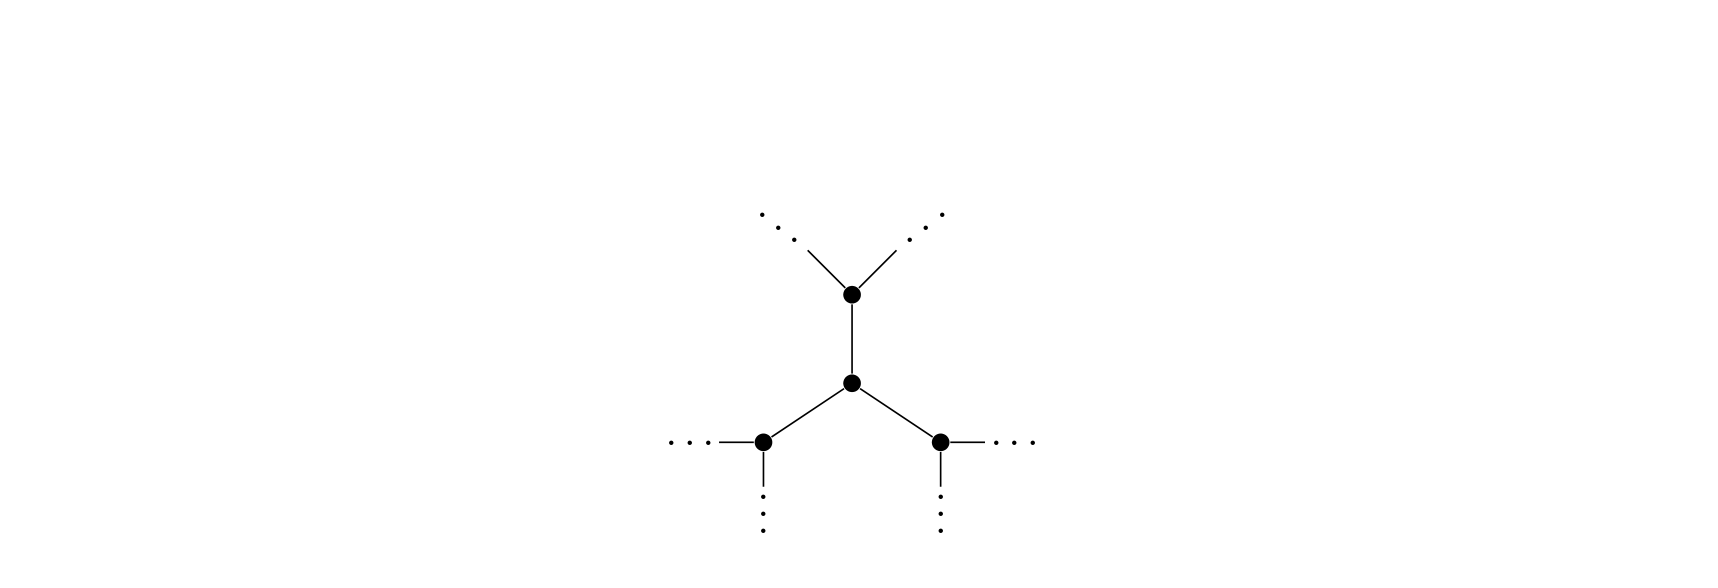
\includegraphics[width=0.4\textwidth]{figure9-1.png}
  \caption{$\mathrm{PGL}_2$在$\Q_2$上的建筑是一棵$3$-正则树。图中画出了构成$\mathrm{PGL}_2/\Q_2$建筑的无限$3$-正则树的$4$个顶点。完整的建筑见图 9.2。（原文 p.~131，Figure 9.1）}
  \label{fig:9-1}
\end{figure}

\begin{figure}[htbp]
  \centering
  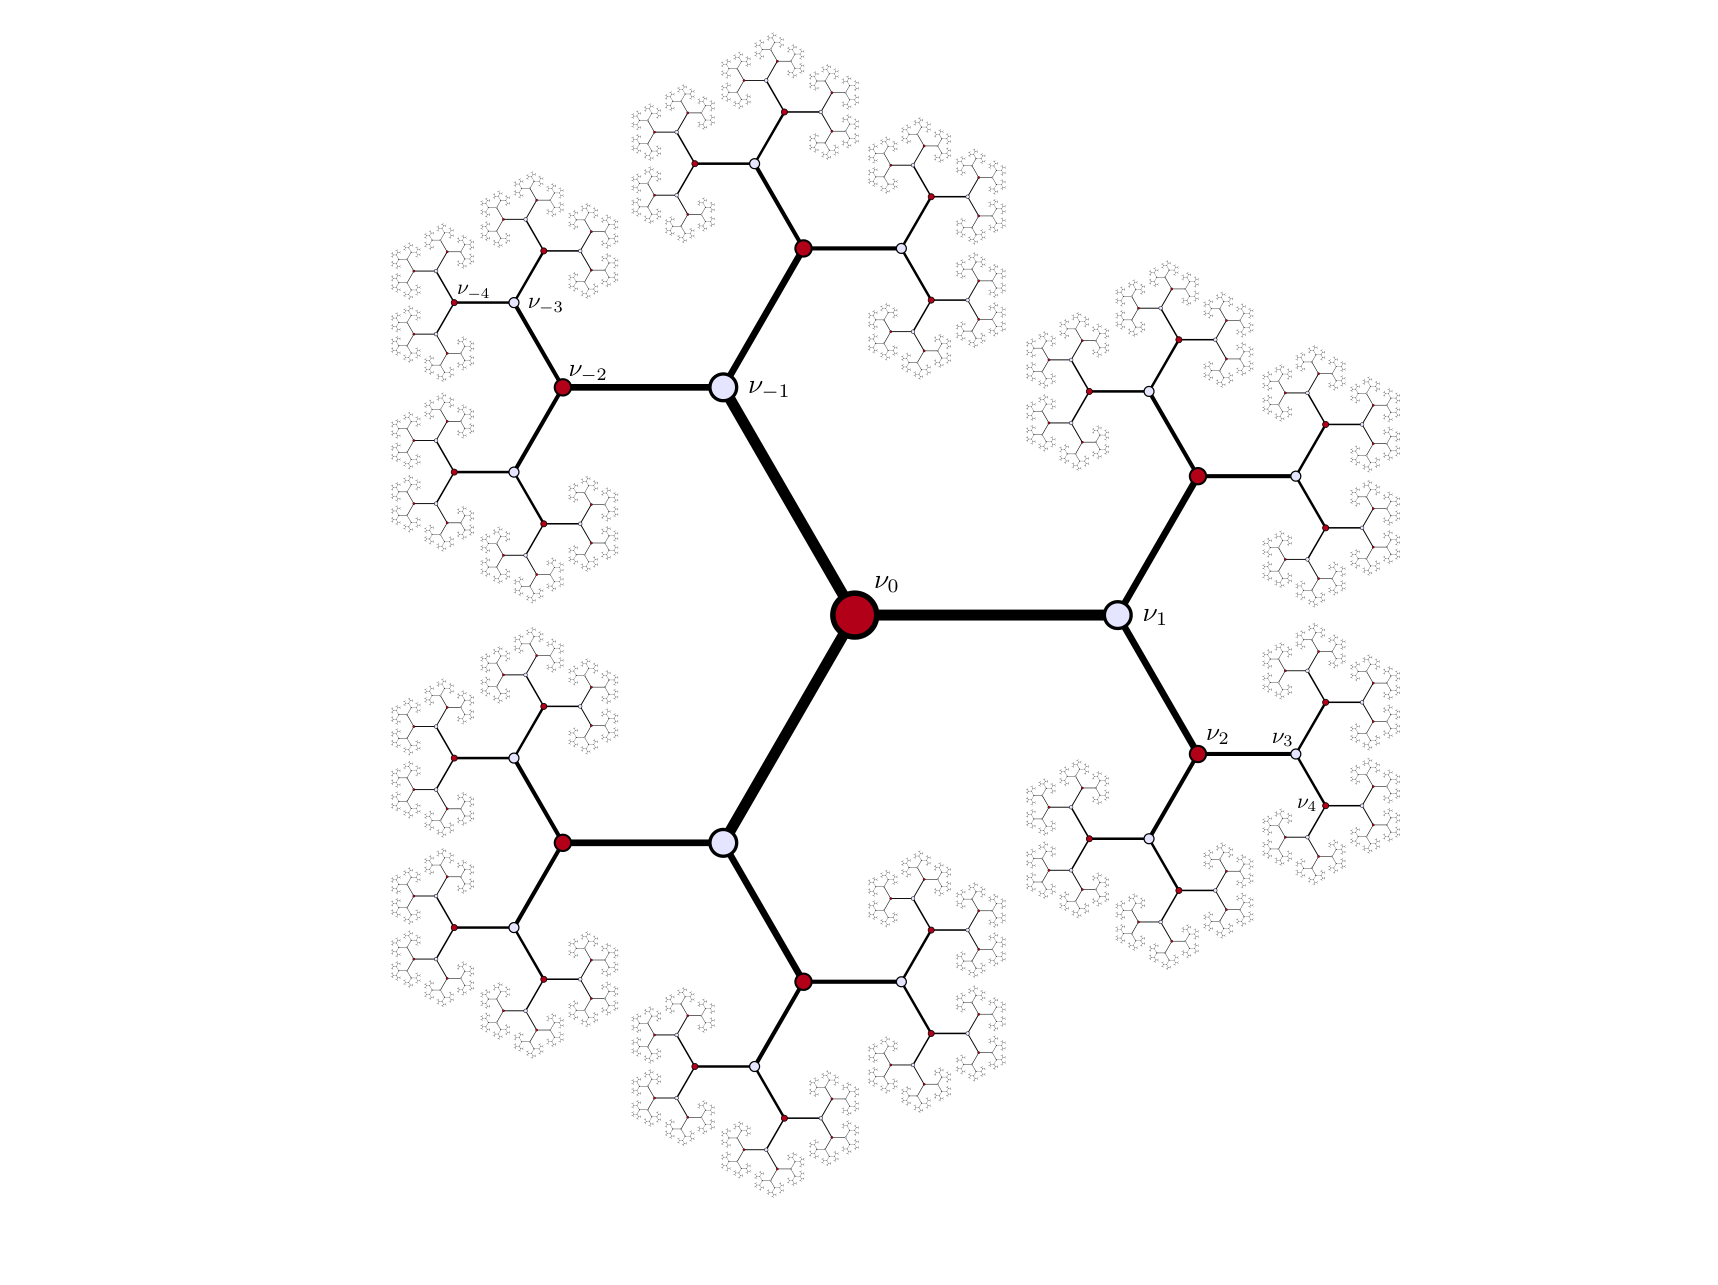
\includegraphics[width=0.78\textwidth]{figure9-2.png}
  \caption{$\mathrm{PGL}_2$在$\Q_2$上的建筑。$G(\cO)$-轨道是围绕中心的同心“圆环”状顶点集，并以颜色区分。图取自 [Cas14]。（原文 p.~131，Figure 9.2）}
  \label{fig:9-2}
\end{figure}

% ---------------------------------------------------------------- 原文 p.132
这也称为$G$的仿射 Grassmann 流形。这是双曲空间的$p$-进类比。想法是顶点在无穷远处聚集，正如双曲空间的圆盘模型。美妙之处在于，双曲空间的许多标准特征都反映在这棵树的几何中。

双商
\begin{equation}\tag{9.127}
G(\cO)\backslash G(K)/G(\cO)
\end{equation}
对应于这棵建筑上的$G(\cO)=\mathrm{PGL}_2(\Z_p)$-轨道。回忆在实际的双曲空间$\mathbb H$中，$i$的稳定化子是$G(\cO)$，其他$G(\cO)$-轨道由它们到某点$i$的距离标记。这里我们有类似的图景。$G(\cO)$是$\Q_p^{2}$中模去伸缩的$\Lambda_0=\Z_p^{2}$的稳定化子，即图 9.1 中间这个点的稳定化子等于$G(\cO)$。然后其他轨道同样是这些同心“圆环”，由到$\Lambda_0$的距离标记，只是现在距离由树度量给出，即边数。所以轨道对应于$\Z_{+}$。

于是 Hecke 算子如下。“树 Laplacian”$T_{p^n}$把$G(K)/G(\cO)$上的函数$f$送到在固定距离$n$的点上取平均的函数：
\begin{equation}\tag{9.128}
(T_{p^n}f)(v)=\sum_{\operatorname{dist}(w,v)=n}f(w).
\end{equation}
同样地，这些全部交换，而且我们发现这些算子的代数就是多项式代数$\C[T_p]$。

所以只要把$\Bun_G$写成
\begin{equation}\tag{9.129}
\Bun_G=G(F)\backslash\prod{}^{\prime}G(K_x)/G(\cO_x),
\end{equation}
我们就得到所有这些代数的作用，且它们彼此交换。目前还不清楚的是：这些代数每一个自身是交换的。
% [Tutor Note: 末句是本章的悬念，也是后续各章的主题：局部 Hecke 代数$\C_c[G(\cO)\backslash G(K)/G(\cO)]$的交换性由 Satake 同构（定理 8）保证，但“整体”Hecke 代数的交换性需要 TFT/几何 Langlands 的解释。阅读时勿把两个层级的交换性混为一谈。]

% ============================================================================
%  第 10 章 拓扑场论中的算子与缺陷
%  译自 Ben-Zvi 讲义第 133–178 页（PDF 页码）
% ============================================================================
\chapter{拓扑场论中的算子与缺陷}\label{ch:10}

\begin{keytakeaways}
本章把“态—算子—缺陷”的量子力学直觉提升为拓扑场论的范畴语言。核心观点是：一个 $n$ 维 TFT 就是从配边范畴到对称幺半范畴的函子 $\mathcal{Z}$——$(n-1)$-维流形给出对象（态空间），$n$ 维配边给出态射；正定向点给 $V$，负定向点给对偶 $V'$，而 1 维 TFT 的公理（求值与余求值满足的“Zorro 之痕”关系）自动蕴含 $V$ 可对偶且有限维。于是“算子”被解释为把正点与负点并置的配边，或等价地解释为两个一维理论之间的界面；界面的复合由“碰撞”配边给出，这为 Hecke 代数、Bernstein 中心与谱分解提供了统一的物理来源。二维 Yang--Mills 理论（有限群）是贯穿全章的模型：边界条件对应表示，局部算子给出交换代数、真空模空间与 B-模型。最后用带奇点的配边假设处理线算子与曲面缺陷，说明高维时局部算子交换、线算子在 3 维为辫状、4 维及以上为对称；并把这套结构落到四维拓扑 Maxwell 理论与几何 Langlands 的 Hecke 对应上。
\end{keytakeaways}

% ============================================================================
\section{态空间}\label{sec:10-1}

\begin{sectionkey}
一维 TFT 就是拓扑量子力学；其配边范畴公理（求值与余求值的 Zorro 关系）恰好等价于“态空间可对偶且有限维”。这为后文“态即边界条件、算子即界面”的整套语言奠定基础。
\end{sectionkey}

一维量子场论就是量子力学。于是我们有一个态空间，即 Hilbert 空间 $H$，并且它被一个可观测量的结合代数 $A$ 所作用。通常 $A$ 由 $H$ 上的全部算子组成。示意性的图像是：$H$ 由某一确定时刻的全部态组成。于是，若有一个态 $\psi\in H_{t_0}$，我们可以在 $t_0$ 之后的某个时刻放置一个算子 $\mathcal{O}$，而经过该算子之后我们得到一个新态 $\mathcal{O}*\psi\in H_{t_1}$。心中要有的图像是：
\begin{equation}\tag{10.1}
\begin{array}{ccc}
\psi_0\in H_{t_0} & \xrightarrow{\ \ \mathcal{O}\ \ } & \mathcal{O}*\psi_0\in H_{t_1}
\end{array}
\end{equation}

这一切在\term{拓扑量子力学}{topological quantum mechanics}中都变得容易得多。

一维 TFT（即拓扑量子力学）是一个对称幺半函子：
\begin{equation}\tag{10.2}
\mathcal{Z}\colon \big(\Bord_1^{\mathrm{or}},\sqcup\big)\longrightarrow\big(\Vect_{\C},\otimes\big).
\end{equation}
$\Bord_1^{\mathrm{or}}$ 的对象是 $0$-流形，但它们是 1-定向的：也就是说，我们为 $n$ 维 TFT 画的所有图像都是 $n$ 维的，因为配边带有 $n$ 维的切向结构。换个说法：你面对的不只是一个 $0$-流形，而是某个\emph{定向} $n$-流形的芽。所以这里可以认为对象是附带一个小的定向区间的 $0$-流形。因此只有两个 1-定向的 $0$-流形：
\begin{equation}\tag{10.3}
\bullet\!\!\longrightarrow \qquad\qquad \longleftarrow\!\!\bullet
\end{equation}
于是函子 $\mathcal{Z}$ 把它们送到两个向量空间：
\begin{equation}\tag{10.4}
\mathcal{Z}\big(\bullet\!\!\longrightarrow\big)=V, \qquad\qquad
\mathcal{Z}\big(\longleftarrow\!\!\bullet\big)=V'.
\end{equation}

\begin{srcrem}{49}
$V$ 最终将是我们的态空间。
\end{srcrem}

现在我们要注意的是，TFT 的公理决定了 $V$ 与 $V'$ 之间的一种密切关系。在 $\Bord_1^{\mathrm{or}}$ 中，从这两个对象的不交并到单位（即空的 $0$-流形 $\varnothing_0$）存在一个自然的态射：
\begin{equation}\tag{10.5}
\big(\bullet\!\!\longrightarrow\big)\;\sqcup\;\big(\longleftarrow\!\!\bullet\big)\;\longrightarrow\;\varnothing_0,
\end{equation}
也就是说，它是：
\diageq{10.6}{0.09\textwidth}{p134_d1.png}
函子 $\mathcal{Z}$ 是对称幺半的，因此它把这个配边送到一个函子，我们称之为求值：
\begin{equation}\tag{10.7}
\mathrm{ev}\colon V\otimes V'\longrightarrow \mathcal{Z}(\varnothing_0)=\C.
\end{equation}
我们还有相反的配边：
\diageq{10.8}{0.09\textwidth}{p134_d2.png}
它给出余求值：
\begin{equation}\tag{10.9}
\mathrm{coev}\colon \C\longrightarrow V\otimes V'.
\end{equation}
这些映射满足一个很好的关系，称为\term{Zorro 之痕}{Mark of Zorro}，因为它来自如下配边：
\diageq{10.10}{0.20\textwidth}{p134_d3.png}
分解这个配边，我们看到函子 $\mathcal{Z}$ 把它送到如下复合：
\begin{equation}\tag{10.11}
V\;\xrightarrow{\ 1\otimes\mathrm{coev}\ }\;V\otimes V'\otimes V\;\xrightarrow{\ \mathrm{ev}\otimes 1\ }\;V,
\end{equation}
\diagram[0.13\textwidth]{p134_d4.png}
其中下图满足交换，即这些映射复合成恒等，因为我们可以把那个配边拉直，而它必须诱导 $V$ 上的恒等映射。

% [Tutor Note: 这里（10.11）下方的小弧箭头即 $\mathrm{id}$；Zorro 关系就是“拉直配边”给出的复合等于恒等。方向务必核对：求值 $V\otimes V'\to\C$、余求值 $\C\to V\otimes V'$，两者顺序不能交换，否则得到的不是对偶公理而是它的转置。]

一旦展开定义，这就是用范畴论的方式说 $V$ 是一个\term{可对偶对象}{dualizable object}，其对偶为 $V'$。这蕴含 $V$ 事实上是有限维的，且 $V'=V^{*}$。

我们可以这样总结：有一个自然的求值映射 $V\otimes V^{*}\to\C$，以及一个自然的恒等映射 $\C\to\End(V)$。而对有限维的 $V$ 有 $V\otimes V^{*}\simeq\End(V)$，于是我们有：
\begin{equation}\tag{10.12}
\begin{array}{ccc}
V\otimes V^{*} & \xrightarrow{\ \ \mathrm{ev}\ \ } & \C\\[5pt]
{\scriptstyle \mathrm{Tr}}\Big\downarrow & & \Big\downarrow{\scriptstyle \mathrm{id}}\\[5pt]
\C & \xrightarrow{\ \ \underset{\mathrm{Tr}(\mathrm{id})=\dim(V)}{\sum e_i\otimes e^i}\ \ } & \End(V)
\end{array}
\end{equation}

% [Tutor Note: （10.12）的四个箭头分别是：上边 $\mathrm{ev}$、左边 $\mathrm{Tr}$（从 $V\otimes V^{*}$ 到 $\C$）、右边 $\mathrm{id}$（从 $\C$ 到 $\End(V)$）、下边 $\sum_i e_i\otimes e^{i}$。注意左右两条竖边的方向不同，容易画反；这里 $e_i$ 与 $e^{i}$ 是对偶基，$\mathrm{Tr}(\mathrm{id})=\dim V$ 正是“对偶配对 + 缩并”给出的维数。]

% ============================================================================
\section{算子}\label{sec:10-2}

\begin{sectionkey}
有限维性把“算子”变成配边：$V\otimes V^{*}=\End(V)$ 对应正点与负点的并置，乘法由把两个这样的对象“焊接”起来的配边给出，作用则由“算子贴着态”的配边给出。
\end{sectionkey}

我们已经看到，$\mathcal{Z}$ 把正定向点送到有限维向量空间 $V$，把负定向点送到对偶空间。这个向量空间 $V$ 就是态空间。现在我们要在这幅图像里找到算子。首先，由于 $V$ 是有限维的，我们有 $V\otimes V^{*}=\End(V)$，它由 $V$ 上的全部算子组成。如果你愿意，这就是 $\mathcal{Z}$ 赋予 $\Bord_1^{\mathrm{or}}$ 的如下对象的值：
\begin{equation}\tag{10.13}
\big(\bullet\!\!\longrightarrow\big)\;\sqcup\;\big(\longleftarrow\!\!\bullet\big)\quad=\quad\bullet\!\!\longrightarrow\!\!\bullet\!\!\longrightarrow
\end{equation}

\begin{srcrem}{50}
眼下我们把这个配边看作式~(10.13) 的左端。下文式~(10.20) 将使用其右端的解读。
\end{srcrem}

代数结构来自如下配边：
\diageq{10.14}{0.20\textwidth}{p135_d3.png}
因为 $A$ 把它送到一个乘法映射：
\begin{equation}\tag{10.15}
\End(V)\otimes\End(V)\longrightarrow \End(V).
\end{equation}
$\End(V)$ 在 $V$ 上的作用来自如下配边：
\diageq{10.16}{0.19\textwidth}{p135_d4.png}
因为 $\mathcal{Z}$ 把它送到一个映射：
\begin{equation}\tag{10.17}
\End(V)\otimes V\longrightarrow V.
\end{equation}

% [Tutor Note: 原文此处写“因为 $A$ 把它送到一个乘法映射”，其中 $A$ 是上一节的可观测量代数；按上下文这里应为 $\mathcal{Z}$，即函子把配边送到乘法映射。记号混用是原稿的笔误，照译并在此指出。]

% ============================================================================
\section{界面}\label{sec:10-3}

\begin{sectionkey}
界面是“两种理论之间的态射”，严格化为双色（蓝/红）配边上的函子。一维情形下，双色场论恰好等价于“一对向量空间 $V,W$ 加上一个映射 $\mathcal{O}\colon W\to V$”，于是态射就是算子、态就是 $\C\to V$ 的界面。
\end{sectionkey}

我们可以用界面的语言同时表述算子与态。设 $V$ 与 $W$ 是两个有限维向量空间。于是可以构造 TFT $\mathcal{Z}_V$ 与 $\mathcal{Z}_W$，其中 $\mathcal{Z}_V$ 把正点送到 $V$，$\mathcal{Z}_W$ 把正点送到 $W$。现在我们来定义 $\mathcal{Z}_V$ 与 $\mathcal{Z}_W$ 之间\term{界面}{interface}（即态射）的概念。

一个界面被编码在\term{双色场论}{bipartite field theory}的概念中，后者是一个函子 $\Bord_1^{\mathrm{or,bi}}\to\Vect$，并满足下面概述的若干性质。范畴 $\Bord_1^{\mathrm{or,bi}}$ 与 $\Bord_1^{\mathrm{or}}$ 相同，只是对象与态射都是\emph{双色流形}。这意味着流形被分解为两部分，我们称之为“蓝”部与“红”部。例如：
\begin{equation}\tag{10.18}
\textcolor{blue}{\rule[0.55ex]{2.6em}{1.1pt}}\!\!\bullet\!\!\textcolor{red}{\rule[0.55ex]{2.6em}{1.1pt}}
\end{equation}
是一个双色 $1$-流形。于是有些双色流形全蓝，有些全红，有些两色兼有。我们对双色场论 $\mathcal{Z}$ 的一项要求是：在完全为红的流形 $R$ 上，$\mathcal{Z}(R)=\mathcal{Z}_V(R)$；在完全为蓝的流形 $B$ 上，$\mathcal{Z}(B)=\mathcal{Z}_W(B)$。然后还有被分解为蓝部与红部的流形。上面的例子给出从蓝色区间到红色区间的一个配边，因此它给出一个映射 $\mathcal{O}\colon W\to V$。所以这个双色流形是我们加进范畴中的一种新的配边。

现在可以证明：这样的双色一维场论对应于一对向量空间 $V,W$，并配有一个映射：
\begin{equation}\tag{10.19}
\mathcal{O}\colon W\longrightarrow V.
\end{equation}
要点是：我们得到一个场论的范畴（态射即界面），它恰好等价于向量空间的范畴。我们要把它想成：$V$ 与 $W$ 沿一个界面相遇，在那里关于 $V$ 的量子力学变成关于 $W$ 的量子力学。

\begin{srcex}{50}
若 $V=W$，则自界面由算子 $\mathcal{O}\in\End(V)$ 标记。其想法是：在两条线相遇的地方，看起来正是 (10.13) 的右端：
\begin{equation}\tag{10.20}
\bullet\!\!\longrightarrow\!\!\bullet\!\!\longrightarrow
\end{equation}
\end{srcex}

同样，一个态 $\psi\in V$ 等同于一个映射 $\C\to V$，它把 $1\mapsto\psi\in V$。于是我们可以把它写成从“平凡”理论 $\mathcal{Z}_{\C}$ 到 $\mathcal{Z}_V$ 的一个界面。我们不去画平凡理论，于是可以把态看成一种新的边界条件：
\begin{equation}\tag{10.21}
\overset{\textstyle V}{\underset{\textstyle \psi}{\bullet\!\!-\!\!-\!\!-\!\!-\!\!-}}
\end{equation}
这里可以想象平凡理论位于 $\psi$ 的左侧。

% [Tutor Note: 界面方向的约定最容易出错：$\mathcal{O}\colon W\to V$ 表示“把蓝（$W$）接到红（$V$）”，与 (10.13) 中“正点 $\sqcup$ 负点”的解读一致；若把 $V$ 与 $W$ 的位置对调，得到的就是 $\mathcal{O}^{T}\colon V^{*}\to W^{*}$ 而不是同一个界面。另外 (10.21) 中“平凡理论在左侧”对应 $\C\to V$ 的箭头方向，画图时不要把它画成 $V\to\C$。]

\begin{flushright}\small 第 20 讲；2021 年 4 月 8 日\end{flushright}

% ============================================================================
\section{二维 TFT}\label{sec:10-4}

\begin{sectionkey}
从一维升到二维，配边成为 2-范畴：对象是 0-流形、1-态射是带 2 维切向结构的区间、2-态射是带角的曲面。二维 TFT 把闭曲面送到数、把 1-流形送到向量空间；而“边界条件”之所以天然构成范畴，是因为存在“界面之间的界面”。
\end{sectionkey}

我们将讨论二维 TFT，着眼于研究算子与缺陷。特别地，我们希望看到 TFT 的内在结构，以及它如何反映在表示论中。

\subsection{基本设定}\label{sec:10-4-1}

设 $\Bord_2^{\mathrm{or}}$ 为定向配边 2-范畴。其对象可以看作带 2 维切空间的 $0$-流形。1-态射是 $0$-流形之间的 $1$-流形配边，我们仍把它视为带有 2 维切空间。我们给配边装备的这个切空间，既是一种记录维数的方式，也是一种指定定向、标架以及其他切向结构的方式。例如，我们可以把一个 $1$-态射画成：
\diageq{10.22}{0.18\textwidth}{p136_d2.png}

2-态射是带角的 $2$-流形。例如，下面是上述 $1$-态射到自身的一个 $2$-态射：
\diageq{10.23}{0.18\textwidth}{p137_d1.png}
我们不久前在图~6.3 中见过同一个配边。

这个 $2$-范畴的重要之处在于：它关于不交并运算是\term{对称幺半}{symmetric monoidal}的，单位由空集 $\varnothing$ 给出。

\begin{srcrem}{51}
配边成族出现，也就是带有分类空间。例如，亏格 $g$ 的闭曲面可以看成从空的 $1$-流形 $\varnothing_1$ 到自身的配边。这些配边构成一个族，由 $\mathrm{B}\,\mathrm{Diff}(\Sigma^{g})$ 给出，而后者等同于亏格 $g$ 曲线的模空间 $\mathcal{M}_g$。
\end{srcrem}

\term{二维 TFT}{two-dimensional TFT}是对称幺半函子：
\begin{equation}\tag{10.24}
\mathcal{Z}\colon\big(\Bord_2^{\mathrm{or}},\sqcup,\varnothing\big)\longrightarrow\big(\mathcal{C},\otimes,1\big).
\end{equation}
这是定义，但我们早已知道二维 TFT 应当给曲面赋数：$\mathcal{Z}(\Sigma)\in\C$；给 $1$-流形赋向量空间 $\mathcal{Z}(N)\in\Vect_{\C}$。这还可以换一种说法。如果我们截断到 $\Bord_{[1,2]}^{\mathrm{or}}$，即不包含角，那么我们实际上应当落到：
\begin{equation}\tag{10.25}
\Bord_{[1,2]}^{\mathrm{or}}\longrightarrow \Vect_{\C}.
\end{equation}
但描述这个截断配边范畴的另一种方式是：空 $0$-流形的自同态
\begin{equation}\tag{10.26}
\End(\varnothing_0),
\end{equation}
也就是说，如果我们想在顶层得到数、在下一层得到向量空间，那么就应当有
\begin{equation}\tag{10.27}
\Vect_{\C}=\End(1_{\C}).
\end{equation}
现在，除这个截断函子之外，要确定 $\mathcal{Z}$ 还需要的额外数据只是一个对象 $\mathcal{Z}(\mathrm{pt})\in\mathcal{C}$。但我们可以用一种典范的方式让这一点更具体。给定任意对象 $C\in\mathcal{C}$，可以附上一个 $\C$-线性范畴：
\begin{equation}\tag{10.28}
\Hom(1_{\C},C).
\end{equation}
我们在一个 $2$-范畴中，所以这确实构成一个范畴；它是 $\C$-线性的，因为可以与单位的自同态作前复合。于是若你有一个函子 $\mathcal{Z}\colon\Bord_2\to\mathcal{C}$，它就提升为：
\begin{equation}\tag{10.29}
\begin{array}{ccc}
\Bord_2 & \longrightarrow & \mathcal{C}\\[3pt]
& \searrow & \Big\downarrow\\[3pt]
& & \mathrm{Cat}_{\C}
\end{array}
\end{equation}
实践中 $\mathcal{C}\to\mathrm{Cat}_{\C}$ 要么是等价，要么是全嵌入。

\begin{srcex}{51}
设 $\mathcal{C}$ 是结合代数的 Morita $2$-范畴。也就是说：对象是结合代数，$A$ 与 $A'$ 之间的 $1$-态射是双模 ${}_A B_{A'}$，$2$-态射是双模之间的映射。它作为 $\C$-线性范畴的全子范畴嵌入，嵌入方式是把一个结合代数送到它的模范畴。
\end{srcex}

% [Tutor Note: 这里 $\mathrm{Cat}_{\C}$ 是 $\C$-线性范畴的 $2$-范畴；(10.29) 的三角形表示“$\Bord_2\to\mathcal{C}$ 可以提升为取值在 $\mathrm{Cat}_{\C}$ 中的函子”，提升的构造就是 (10.28)：$C\mapsto\Hom(1,C)$。注意 $\Hom(1,C)$ 是范畴而不是集合，这是 $2$-范畴与普通范畴的关键差别。]

\subsection{界面与高阶范畴}\label{sec:10-4-2}

现在我们要用 TFT 的语言、而非范畴论的语言来解释这一运算。回忆我们有 TFT 之间\term{界面}{interface}的概念，它是拓扑场论之间的一种“映射”。为此我们使用双色（bipartite）$2$-流形。设 $\mathcal{Z}$ 与 $\mathcal{W}$ 是两个取值在同一范畴中的场论：
\begin{equation}\tag{10.30}
\mathcal{Z},\,\mathcal{W}\colon \Bord_2\longrightarrow \mathcal{C}.
\end{equation}
从 $\mathcal{Z}$ 到 $\mathcal{W}$ 的态射是双色范畴 $\Bord_2^{\mathrm{bi}}$ 上的一个函子。我们不给出正式定义，但一个闭的双色 $2$-流形实际上就是带“红部”与“蓝部”的闭 $2$-流形，如图~10.1。想法是：这个理论通过把 $\mathcal{Z}$ 作用到红色流形上、把 $\mathcal{W}$ 作用到蓝色流形上而给出，此外还有来自这些被分解的流形各被赋予什么的额外信息。我们可以通过记录定向来跟踪它是态射 $\mathcal{Z}\to\mathcal{W}$ 还是 $\mathcal{W}\to\mathcal{Z}$。

\begin{figure}[htbp]
  \centering
  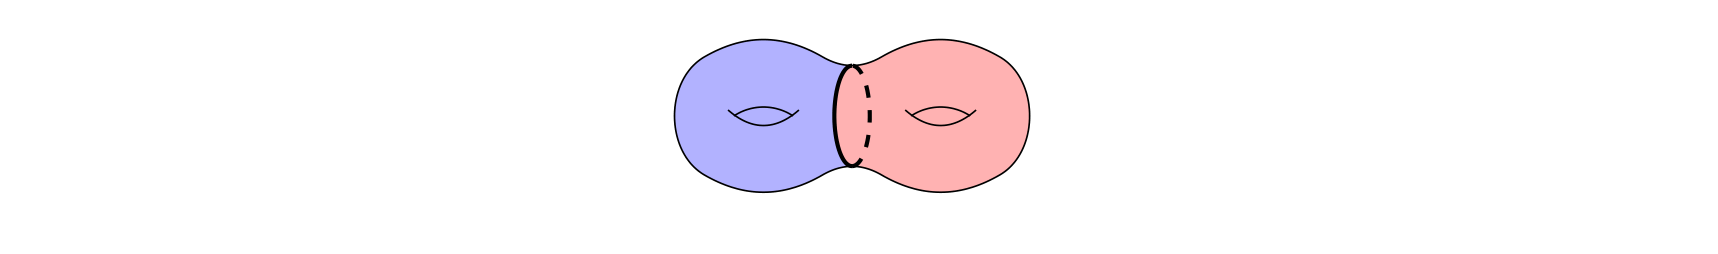
\includegraphics[width=0.26\textwidth]{figure10-1.png}
  \caption{一个闭的双色 $2$-流形。（原文 p.~138，Figure 10.1）}
  \label{fig:10-1}
\end{figure}

利用某种带奇点的配边假设版本，这些界面对应于映射：
\begin{equation}\tag{10.31}
\mathcal{Z}(\mathrm{pt})\longrightarrow\mathcal{W}(\mathrm{pt}).
\end{equation}
这个态射来自双色配边：
\begin{equation}\tag{10.32}
\text{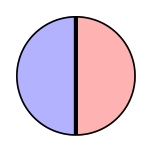
\includegraphics[width=0.045\textwidth]{p138_d2.png}}\;=\;
\textcolor{blue}{\rule[0.55ex]{1.6em}{1.1pt}}\!\!\bullet\!\!\textcolor{red}{\rule[0.55ex]{1.6em}{1.1pt}},
\end{equation}
于是整个结构由 $\mathcal{Z}$、$\mathcal{W}$ 以及理论赋予这个配边的值决定。

设 $C=\mathcal{Z}(\mathrm{pt})$。则 $\Hom(1,C)$ 对应于与 $1$ 相伴的平凡理论和理论 $\mathcal{Z}$ 之间的界面。我们可以把它们画成 $\mathcal{Z}$ 与“空”之间的界面：
\diageq{10.33}{0.16\textwidth}{p138_d3.png}
这就是所谓的 $\mathcal{Z}$ 的\term{边界条件}{boundary condition}或边界理论。

所谓“$\mathcal{C}$ 的对象”（其中 $C\in\mathcal{C}$），按定义指的是底范畴 $\Hom(1,C)$ 的对象。它们等同于态射 $1\to\mathcal{Z}_C$，而后者等同于 $\mathcal{Z}_C$ 的边界理论。$\mathcal{Z}_C$ 的边界理论实际上意味着：我们把函子 $\mathcal{Z}$ 延拓到带一个标记边界分支的 $2$-流形上。也就是说，我仍然看 $2$-流形，但其中一个边界分支标以 $B$，而流形内部标以 $\mathcal{Z}$。

\begin{srcrem}{52}
这是一般构造的一个特例，我们之后会更详细地看到。即：对 TFT $\mathcal{Z}$ 的余维 $k$ 的\term{缺陷理论}{defect theory}意味着把 $\mathcal{Z}$ 从 $n$-流形延拓到带嵌入的、被标记的余维 $k$ 子流形的 $n$-流形上。把这样的延拓记作 $\mathcal{D}_k$，于是我们可以用字母 $\mathcal{D}$ 标记这些子流形。
\end{srcrem}

\begin{figure}[htbp]
  \centering
  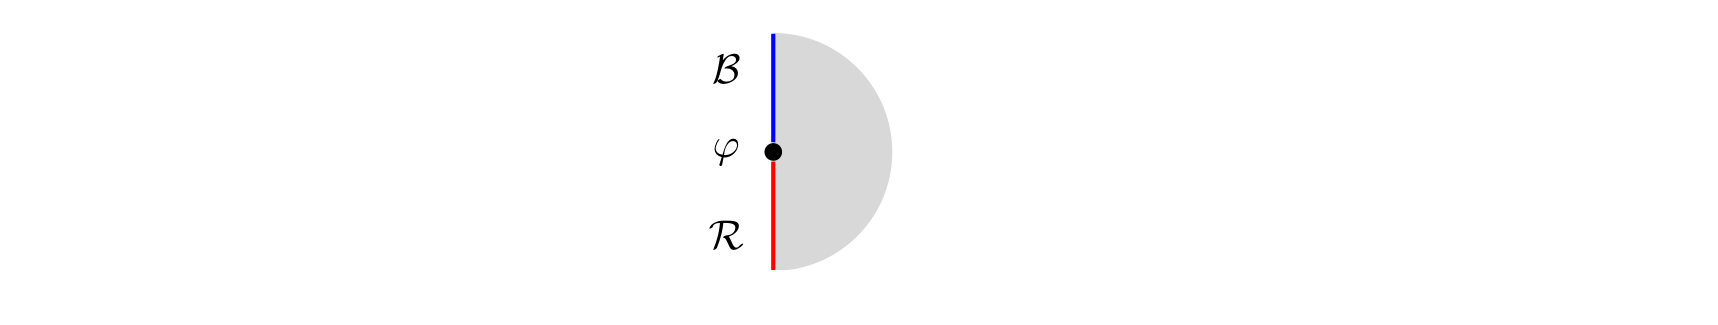
\includegraphics[width=0.24\textwidth]{figure10-2.png}
  \caption{两个界面之间的界面。这是一个带角配边，对应于边界条件 $\mathcal{B},\mathcal{R}\in\Hom(1,\mathcal{Z}(\mathrm{pt}))$ 之间的映射 $\varphi\colon\mathcal{B}\to\mathcal{R}$。（原文 p.~139，Figure 10.2）}
  \label{fig:10-2}
\end{figure}

如果我们在余维 $1$，那么子流形把流形分成两部分，即它是双色流形，于是我们可以用不同的理论标记任一部分。或者我们可以把两部分都标以 $\mathcal{Z}$，这时得到 $\End(\mathcal{Z})$。如果一侧标以平凡理论，就得到边界条件。这里真正发生的是：$0$-球面是不连通的，所以余维 $1$ 子流形的链环不连通，于是每个分支上做什么存在选择。

要点是：二维 TFT $\mathcal{Z}$ 的边界条件构成一个范畴，尽管 $\mathcal{Z}(\mathrm{pt})$ 本身可能不是范畴。任何 $\mathcal{B}\in\Hom(1,\mathcal{Z}(\mathrm{pt}))$ 对应于 $\mathcal{Z}$ 与平凡理论之间的一个界面。作为 $2$-范畴中 $\Hom$ 的对象，意味着它们按定义就构成一个范畴。但这些对象之所以是范畴的对象，其物理原因是存在界面之间的界面，如图~10.2。这对应于边界条件 $\mathcal{B},\mathcal{R}\in\Hom(1,\mathcal{Z}(\mathrm{pt}))$ 之间的映射 $\mathcal{B}\to\mathcal{R}$。

图~10.2 是从如下对象出发的新的带角配边：
\begin{equation}\tag{10.34}
\textcolor{black}{\rule[-1.1ex]{0.8pt}{1.1ex}}\!\!\bullet\!\!\textcolor{red}{\rule[-1.1ex]{0.8pt}{1.1ex}}
\quad\longrightarrow\quad
\textcolor{blue}{\rule[-1.1ex]{0.8pt}{1.1ex}}\!\!\bullet\!\!\textcolor{red}{\rule[-1.1ex]{0.8pt}{1.1ex}}
\end{equation}
这是完全合格的带标记边界的 $1$-流形，于是理论把它们赋予某个向量空间。所以从 $\mathcal{B}$ 到 $\mathcal{R}$ 的界面全体构成一个向量空间。这个向量空间已经是理论的一部分。特别地，它就是如下赋值：
\begin{equation}\tag{10.35}
\mathcal{Z}\big(\textcolor{blue}{\bullet}\!\!\longrightarrow\!\textcolor{red}{\bullet}\big).
\end{equation}
我们可以把这个区间看成奇点的\term{链环}{link}。这些向量空间就是 $\Hom(\mathcal{B},\mathcal{R})$。配边：
\diageq{10.36}{0.17\textwidth}{p139_d2.png}
或等价的“马裤对”（pair of chaps）配边：
\diageq{10.37}{0.20\textwidth}{p140_d1.png}
二者都诱导复合映射：
\begin{equation}\tag{10.38}
\Hom(\mathcal{B},\mathcal{G})\otimes\Hom(\mathcal{G},\mathcal{R})\longrightarrow\Hom(\mathcal{B},\mathcal{R}).
\end{equation}
因此这些向量空间像范畴中的态射一样复合。

同样的想法在任意维数都成立。对 $n$ 维 TFT，我们可以构造边界理论的 $(n-1)$-范畴，其中对象是边界条件，$1$-态射是边界条件之间的界面，$2$-态射是界面之间的界面，如此一直进行到第 $(n-1)$ 层，因为理论是 $n$ 维的。

% [Tutor Note: 这里是全章第一个容易混淆的地方：$\mathcal{Z}(\mathrm{pt})$ 可能不是范畴，但它的“边界条件”却按定义构成范畴 $\Hom(1,\mathcal{Z}(\mathrm{pt}))$。“界面之间的界面”之所以存在，是因为余维 1 子流形的链环是 $S^{0}$（两个点），两个端点可以各自独立地选择边界条件。(10.34) 中的颜色正是标记两个端点所接的边界条件，复合则由 (10.37) 的“马裤对”配边给出。]

\subsection{有限群的二维 Yang--Mills 理论}\label{sec:10-4-3}

这也称为无扭转的 \term{Dijkgraaf--Witten 理论}{untwisted Dijkgraaf--Witten theory}。设 $G$ 是有限群。于是我们定义一个二维 TFT：
\begin{equation}\tag{10.39}
\mathcal{Z}_G\colon \Bord_2^{\mathrm{or}}\longrightarrow \mathrm{Cat}_{\C},
\end{equation}
其构造方式是把流形上 $G$-局部系统的空间线性化。

这将是一个\term{拉格朗日场论}{Lagrangian field theory}，意思如下。我们有这个配边范畴 $\Bord_2^{\mathrm{or}}$，然后从它出发有一个场的构造，取值落在某种几何对象（如群胚）中，然后我们再线性化（例如取层），落到 $\mathrm{Cat}_{\C}$ 中：
\begin{equation}\tag{10.40}
\begin{array}{ccccc}
\Bord_2^{\mathrm{or}} & \xrightarrow{\ F\ } & \mathrm{Grpd} & \xrightarrow{\ \mathrm{Shv}\ } & \mathrm{Cat}_{\C}\\[4pt]
& \searrow & & \swarrow & \\
& & \scriptstyle \mathcal{Z}=\mathrm{Shv}(F(-)) & &
\end{array}
\end{equation}
若 $\Sigma$ 是闭的 $2$-流形，则 $\mathcal{Z}_G(\Sigma)$ 是 $\Sigma$ 上 $G$-局部系统的个数。回忆 $G$-局部系统由下式给出：
\begin{equation}\tag{10.41}
\Loc_G\Sigma=\{\pi_1\Sigma\to G\}\big/\!\sim,
\end{equation}
但当我们数它们时，要按自同构加权：
\begin{equation}\tag{10.42}
\mathcal{Z}_G(\Sigma)=\sum_{P\in\Loc_G\Sigma}\frac{1}{|\Aut(P)|}.
\end{equation}
若 $N^1$ 是 $1$-流形，我们赋予：
\begin{equation}\tag{10.43}
\mathcal{Z}_G\big(N^1\big)=\C\big[\Loc_G N\big],
\end{equation}
这里我们只是把 $\Loc_G N$ 看作有限群胚。若 $P^0$ 是 $0$-流形，则
\begin{equation}\tag{10.44}
\mathcal{Z}_G\big(P^0\big)=\Vect\big(\Loc_G P^0\big).
\end{equation}

例如，
\begin{equation}\tag{10.45}
\mathcal{Z}_G\big(S^1\big)=\C\big[\Loc_G S^1\big]=\C\left[\frac{G}{G}\right],
\end{equation}
它们是\emph{类函数}。对零维流形 $\mathrm{pt}$ 我们有：
\begin{align}
\mathcal{Z}_G(\mathrm{pt})&=\Vect\big(\Loc_G(\mathrm{pt})\big)\tag{10.46}\\
&=\Vect\big(\mathrm{pt}/G\big)\tag{10.47}\\
&=\Rep(G).\tag{10.48}
\end{align}
设 $M$ 是从 $N_{\mathrm{in}}$ 到 $N_{\mathrm{out}}$ 的配边。取 $\Loc_G$ 给出群胚的对应（span，即双拉回图）：
\begin{equation}\tag{10.49}
\begin{array}{ccc}
& \Loc_G M &\\[4pt]
\swarrow & & \searrow\\[4pt]
\Loc_G N_{\mathrm{in}} & & \Loc_G N_{\mathrm{out}}
\end{array}
\end{equation}
在这些群胚上取函数给出：
\begin{equation}\tag{10.50}
\pi_{\mathrm{out},*}\pi_{\mathrm{in}}^{*}\colon \C\big[\Loc_G N_{\mathrm{in}}\big]\longrightarrow\C\big[\Loc_G N_{\mathrm{out}}\big].
\end{equation}
这就是流形之间的配边如何变成相应函数空间之间的映射。

\textbf{问题 4.} 如何看出 $G$ 的\emph{表示}？

抽象地说我们有 $\mathcal{Z}_G(\mathrm{pt})=\Rep(G)$。于是表示 $V\in\Rep(G)$ 等同于 $\mathcal{Z}_G(\mathrm{pt})$ 的一个对象，而后者等同于一个函子 $\Vect\to\Rep(G)$，它把 $\C$ 送到 $V$。也就是说，这是从平凡理论到 $\mathcal{Z}_G$ 的一个界面，即 $\mathcal{Z}_G$ 的一个边界条件。

但这与“带颜色的边界”有什么关系？给定 $G$ 的表示 $V$（我们把它想成“红色”），我们可以把 $\mathcal{Z}_G$ 延拓到带红色边界分支的流形上。例如，我们有一种新的 $1$-配边：
\begin{equation}\tag{10.51}
\textcolor{red}{\bullet}\!\!-\!\!-\!\!-\!\bullet
\end{equation}
它对应于对象 $V\in\mathcal{Z}_G(\mathrm{pt})$。

同样，一个边界分支被标为红色的柱面给出 $\mathcal{Z}_G(S^1)$ 的一个元素。这个元素恰好是 $V$ 的\term{特征}{character}：$\chi_V\in\C\big[G/G\big]$。

物理的解释如下。$V\in\Rep(G)$ 当然是一个向量空间，所以我们可以把它看成定义拓扑量子力学理论的态空间。但把它变成表示，意味着我们把一维理论\emph{耦合}到了体（bulk）规范理论 $\mathcal{Z}_G$ 上。所以我们考虑的是一个量子力学理论，它生活在某些 $1$-流形上，而这些 $1$-流形是某个体的边界，在那个体上我们有理论 $\mathcal{Z}_G$。

\begin{srcex}{52}
回忆正则表示 $\mathrm{Reg}=\C[G]$。它对应于 $\mathcal{Z}_G$ 的 Dirichlet 边界条件。平凡表示 $\C$ 对应于 Neumann 边界条件。
\end{srcex}

我们对这些边界条件能做的主要事情，是讨论它们之间的界面。于是，如果我有一个表示 $V$，以及一个蓝色的表示 $W$，那么一个界面：
\diageq{10.52}{0.15\textwidth}{p142_d1.png}
是 $\mathcal{Z}_G$ 赋予该奇点的链环的那个向量空间的一个元素：
\begin{equation}\tag{10.53}
\mathcal{Z}\big(\textcolor{red}{\bullet}\!\!-\!\!-\!\!-\!\textcolor{blue}{\bullet}\big)=\Hom_{\Rep(G)}(V,W).
\end{equation}
而复合由这种缺陷的碰撞、也就是“马裤对”配边来实现。

现在我们将用场的语言来写边界条件的范畴。带有 $G$ 作用的集合是 $G$ 的表示的一个简单来源，因为 $G\curvearrowright X$ 蕴含 $\C[X]$ 是 $G$-表示。于是我们可以认为边界条件由 $G\curvearrowright X$ 指定，而这里我们暗中把它与表示 $\C[X]$ 联系起来。在体内部我们有 $\Loc_G$，所以总的场空间由 $G$-局部系统连同边界上相伴 $X$-丛的一个截面组成。也就是说，我们把整个曲面映射到 $\mathrm{pt}/G$（这就是为什么得到 $\Loc_G$），然后在标以 $X$ 的边界上，把这个映射提升到 $X/G$：
\begin{equation}\tag{10.54}
\begin{array}{ccc}
& & X/G\\[4pt]
& \nearrow & \Big\downarrow\\[4pt]
\partial\Sigma & \xrightarrow{\qquad} & \mathrm{pt}/G
\end{array}
\end{equation}

\begin{srcex}{53}
若 $X=G$（于是我们考虑的是正则表示），则 $X/G=\mathrm{pt}$，我们考虑的是 $G$-局部系统连同边界上的一个平凡化，这就是 Dirichlet 边界条件。
\end{srcex}

\begin{flushright}\small（原稿批注：transition。）\end{flushright}

% [Tutor Note: 本节有三处约定需要记牢。(1) 边界条件的颜色：红/蓝对应 $V$/$W$，界面方向是 $\Hom_{\Rep(G)}(V,W)$，即 (10.53) 的 $\mathcal{Z}(\text{红}\to\text{蓝})$，不要与反方向的 $\Hom(W,V)$ 混淆。(2) 正则表示 $\C[G]$ 对应 Dirichlet 边界条件、平凡表示 $\C$ 对应 Neumann，这与下一节 $X=G/1$ 对 Dirichlet、$X=\mathrm{pt}=G/G$ 对 Neumann 的“几何”说法是同一件事。(3) 柱面上的元素是特征 $\chi_V$，而不是维数 $\dim V$；维数只在把柱面闭合（再取迹）时出现。]

\begin{flushright}\small 第 21 讲；2021 年 4 月 13 日\end{flushright}

% ============================================================================
\section{拉格朗日理论中的边界条件}\label{sec:10-5}

\begin{sectionkey}
在拉格朗日理论中，边界条件不是“约束”而是“额外结构”：要求到目标 $Y$ 的映射在边界上提升到某个 $Z\to Y$。对有限群 Yang--Mills，$Z\to Y$ 等价于一个 $G$-空间，于是边界条件就是表示；边界条件之间的界面则是 $H\backslash G/K$ 型的双陪集，其复合给出 Hecke 代数。
\end{sectionkey}

基本的图像是：我们考虑从某个时空 $\Sigma$ 到某个目标 $Y$ 的映射理论，即场是映射，而我们对它作线性化。我们可能允许 $\Sigma$ 有边界，然后可以在边界上施加条件。例如，若选取某个子流形 $Z\subset Y$，我们可能要求映射 $\psi\colon\Sigma\to Y$ 把 $\partial\Sigma$ 送到 $Z$：
\begin{equation}\tag{10.55}
\varphi|_{\partial\sigma}\subset Z.
\end{equation}

\begin{srcrem}{53}
为了表述这个问题，我们并不需要 $Z$ 是子流形。我们可以只取某个映射 $Z\to Y$，并要求到 $Y$ 的映射在边界上提升到 $Z$：
\begin{equation}\tag{10.56}
\begin{array}{ccc}
\partial\Sigma & \longrightarrow & Z\\[4pt]
\downarrow & & \downarrow\\[4pt]
\Sigma & \xrightarrow{\ \ \varphi\ \ } & Y
\end{array}
\end{equation}
\end{srcrem}

于是现在我们既有 $\varphi\colon\Sigma\to Y$，又有 $\varphi|_{\partial\Sigma}$ 提升到 $Z$ 的数据：
\begin{equation}\tag{10.57}
\widetilde{\varphi}_{\partial}\colon\partial\Sigma\longrightarrow Z.
\end{equation}

要点是：我们并不是真的在施加一个条件，而是在添加一个映射的额外结构。因此，\emph{边界理论}（boundary theory）可能是比“边界条件”更好的名字。

回忆我们当时研究的是有限群的 Yang--Mills 理论。这是目标为 $Y=\mathrm{pt}/G$ 的理论。于是映射 $\varphi\colon\Sigma\to\mathrm{pt}/G$ 给出 $\Sigma$ 上的一个 $G$-丛。对有限群 $G$，这意味着我们得到的正是 $\Loc_G\Sigma$。

给出一个映射 $Z\to Y=\mathrm{pt}/G$，等价于给出空间 $G\curvearrowright X$。具体地说，对于一个映射：
\begin{equation}\tag{10.58}
\begin{array}{c}
Z\\[-2pt]
\downarrow\\[-2pt]
Y=\mathrm{pt}/G
\end{array}
\end{equation}
我们可以把 $G$-空间 $G\curvearrowright X$ 构造为纤维积：
\begin{equation}\tag{10.59}
\begin{array}{ccc}
X & \longrightarrow & Z\\[4pt]
\downarrow & & \downarrow\\[4pt]
\mathrm{pt} & \longrightarrow & Y=\mathrm{pt}/G
\end{array}
\end{equation}
反之，从一个 $G$-空间 $G\curvearrowright X$ 出发，我们可以构造：
\begin{equation}\tag{10.60}
\begin{array}{c}
Z=X/G\\[-2pt]
\downarrow\\[-2pt]
Y=\mathrm{pt}/G
\end{array}
\end{equation}
因此，一个 $G$-空间 $G\curvearrowright X$ 给出一个边界理论。在此之前我们有
\begin{equation}\tag{10.61}
\Loc_G(\Sigma)=\{\Sigma\to\mathrm{pt}/G\}.
\end{equation}
当 $\Sigma$ 有边界时，我们就可以要求提升到：
\begin{equation}\tag{10.62}
\begin{array}{ccc}
\partial\Sigma & \xrightarrow{\ \ \widetilde{\varphi}_{\partial}\ \ } & X/G\\[4pt]
\downarrow & & \downarrow\\[4pt]
\Sigma & \xrightarrow{\ \ \varphi\ \ } & \mathrm{pt}/G
\end{array}
\end{equation}
这些构成：
\begin{equation}\tag{10.63}
\Loc_G^{X}(\Sigma,\partial\Sigma).
\end{equation}
具体地说，$\varphi$ 对应于一个 $G$-丛：
\begin{equation}\tag{10.64}
\begin{array}{c}
\mathcal{P}\\[2pt]
{\scriptstyle G}\downarrow\\[2pt]
\Sigma
\end{array}
\end{equation}
而提升 $\widetilde{\varphi}_{\partial}$ 的数据等价于相伴 $X$-丛的一个截面：
\begin{equation}\tag{10.65}
\begin{array}{c}
P|_{\partial\Sigma}\times^{G}X\\[2pt]
\downarrow\\[2pt]
\partial\Sigma
\end{array}
\end{equation}
其纤维看起来像 $X$，而过渡数据由作用 $G\curvearrowright X$ 给出。

\textbf{练习 1.} 证明：提升到 $X/G$ 的数据等价于这个相伴 $X$-丛的一个截面。

这个数据也等价于一个 $G$-等变映射 $\mathcal{P}|_{\partial\Sigma}\to X$。

\begin{srcrem}{54}
用物理学的话说，我们是在边界上把 $\Sigma$-模型耦合到 $X$、而体内是 $G$-规范理论。也就是说，在边界上我们有一个低一维的、映入 $X$ 的映射理论，在内部我们有一个关于 $G$-丛的理论，然后把它们拼在一起构造这个耦合理论的场。
\end{srcrem}

\begin{srcex}{54}
若 $X=G/H$，则相伴 $X$-丛的截面 $\mathcal{P}\times^{G}X=\mathcal{P}\times^{G}G/H$ 等同于把 $\mathcal{P}$ 从 $G$ 约化到 $H$。也就是说，这等同于把 $\mathcal{P}$ 写成由某个 $H$-丛诱导出来的。

例如若 $X=G=G/1$，则相伴 $X$-丛的截面等同于 $\mathcal{P}|_{\partial\Sigma}$ 的一个平凡化。这是 Dirichlet 边界条件的规范理论版本。回忆在我们的二维 TFT $\mathcal{Z}_G$（Yang--Mills 理论）中，边界条件对应于 $\Rep(G)$。具体地，一个 $G$-空间给出表示 $\C[X]$。与 $X=G/1$ 相伴的边界条件对应于正则表示 $\C[G]\in\Rep(G)$。

另一个极端是 $X=\mathrm{pt}=G/G$。这就是所谓的 Neumann 条件。它对应于平凡表示 $\C\in\Rep(G)$。
\end{srcex}

% [Tutor Note: (10.55) 中原文写作 $\varphi|_{\partial\sigma}\subset Z$，下标是小写 $\sigma$，而全章其余地方用 $\Sigma$；这应是原稿笔误，照译于此指出。另一个更实质的易错点是“边界条件”的措辞：如作者强调的，它其实是“把映射在边界上提升到 $Z$”的额外结构，而不是对场施加的等式约束；这正是 $X=G/1$ 给出 Dirichlet（平凡化）、$X=\mathrm{pt}$ 给出 Neumann（无附加数据）的原因。]

\subsection{边界条件之间的界面}\label{sec:10-5-1}

现在我们来考虑边界条件之间的界面，在线性化之后它们将对应于表示之间的映射。考虑由表示 $V$ 与 $W$ 给出的两个边界条件。假设 $V$ 来自 $G$-空间 $X_1$，而 $W$ 来自 $G$-空间 $X_2$。那么考虑它们之间的一个界面：
\diageq{10.66}{0.13\textwidth}{p144_d1.png}
这个界面被什么标记？我们已经看到它对应于表示的一个映射；但用 $G$-空间 $X_i$ 来说，我们构造纤维积：
\begin{equation}\tag{10.67}
\begin{array}{ccc}
T & \longrightarrow & X_2/G\\[4pt]
\downarrow & & \downarrow\\[4pt]
X_1/G & \longrightarrow & \mathrm{pt}/G
\end{array}
\end{equation}
而这个界面由如下东西标记：
\diageq{10.68}{0.13\textwidth}{p144_d3.png}

这正是放在这里的自然之物：如果我们在边界的一部分上有一个到 $X_1$ 的提升，在边界的另一部分上有一个到 $X_2$ 的提升，那么在重叠处我们应当提升到某个映射到 $T$ 的东西。

\begin{srcex}{55}
若 $X_1=G/H$ 且 $X_2=G/K$，则 $X/G=\mathrm{pt}/H$ 且 $X_2/G=\mathrm{pt}/K$，于是纤维积为：
\begin{equation}\tag{10.69}
\begin{array}{ccc}
H\backslash G/K & \longrightarrow & \mathrm{pt}/K\\[4pt]
\downarrow & & \downarrow\\[4pt]
\mathrm{pt}/H & \longrightarrow & \mathrm{pt}/G
\end{array}
\end{equation}
也就是说：如果我们在 $\Sigma$ 上有一个 $G$-丛，它在边界的一部分上把结构群从 $G$ 约化到 $H$，在边界的另一部分上从 $G$ 约化到 $K$，那么在重叠处我们就同时约化到 $H$ 和 $K$，而这些由到 $H\backslash G/K$ 的映射给出。也就是说，$\mathrm{pt}/H$ 与 $\mathrm{pt}/K$ 之间的几何/拉格朗日界面由 $H\backslash G/K$ 给出。自界面由 $K\backslash G/K$ 给出。

形象地说我们有：
\begin{equation}\tag{10.70}
H\backslash G/K=\begin{array}{ccc}
& \mathrm{pt}/G &\\[-5pt]
& \bullet &\\[3pt]
\bullet & \longrightarrow & \bullet\\[-6pt]
\mathrm{pt}/H & & \mathrm{pt}/K
\end{array}
\end{equation}
也就是说，我们在内部有一个 $G$-丛，它在一个端点约化为 $H$-丛、在另一个端点约化为 $K$-丛。所有这类丛构成的空间就是 $H\backslash G/K$。
\end{srcex}

\textbf{问题 5.} 这幅图像如何与我们之前的图像联系起来？

我们此前已经稍微看到了这一点，基本想法是：它们通过“从奇点过渡到其链环”联系起来。链环是奇点的一个小管状邻域的边界。所以在这个例子里，我们研究的是 $\mathrm{pt}/H$ 与 $\mathrm{pt}/K$ 之间的界面，而链环是那个绿色区间：
% 校订注：原译文只嵌左侧半圆盘裁件、以中文括注代替右侧绿色区间，且裁件右缘把 pt/G 截成 pt。
% 2026-11-19 由原 PDF p.145 以 400 dpi 重裁整幅（左盘 ≃ 右区间），改为单张图示方程。
\diageq{10.71}{0.46\textwidth}{p145_d2.png}

\subsection{边界条件之间界面的复合}\label{sec:10-5-2}

现在我们要理解界面的复合。Hecke 代数正是以这种方式从物理中获得代数结构的。

物理的图像（称为\term{算子乘积展开}{operator product expansion}，简称 OPE）是：我们有两个界面，但从远处看它看起来像两个界面：
\begin{equation}\tag{10.72}
\text{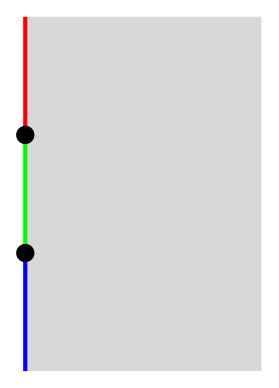
\includegraphics[width=0.11\textwidth]{p146_d1.png}}\quad\simeq\quad
\text{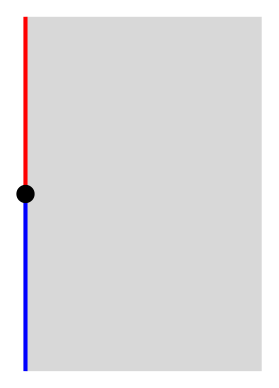
\includegraphics[width=0.11\textwidth]{p146_d2.png}},
\end{equation}
形式上我们可以按 (10.71) 附近的讨论取奇点的链环，得到：
\begin{equation}\tag{10.73}
\text{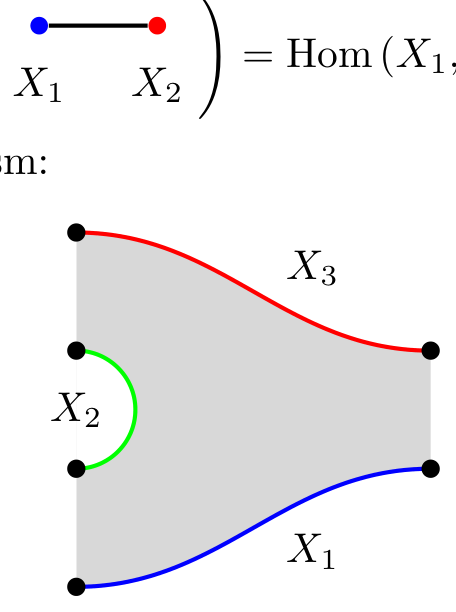
\includegraphics[width=0.22\textwidth]{p146_d3.png}}\;=\;\Hom(X_1,X_2).
\end{equation}
然后“马裤对”配边：
\diageq{10.74}{0.17\textwidth}{p146_d4.png}
诱导出复合映射：
\begin{equation}\tag{10.75}
\Hom(X_1,X_2)\otimes\Hom(X_2,X_3)\longrightarrow\Hom(X_1,X_3).
\end{equation}
Hecke 代数出现在我们考虑三个边界上都约化到 $K$ 的 $G$-丛时：
\begin{equation}\tag{10.76}
\text{（与 (10.74) 相同的“马裤对”配边，只是三个边界 }K,K,K\text{ 都被标以 }K\text{）}
\end{equation}
这幅图给出乘法映射：
\begin{equation}\tag{10.77}
\C[K\backslash G/K]\otimes\C[K\backslash G/K]\longrightarrow\C[K\backslash G/K].
\end{equation}
这就是 Hecke 代数的物理再解释。

\begin{srcex}{56}
若 $K=1$（Dirichlet 边界条件），则 $K\backslash G/K=G$，而这幅图恢复出群代数 $\C G$。
\end{srcex}

\begin{srcex}{57}
若 $K=G$（Neumann 边界条件），则场空间是 $\mathrm{pt}/G$。但 $\C[\mathrm{pt}/G]=\C$，于是 Hecke 代数是 $\End_{\Rep}(\C)=\C$。
\end{srcex}

% [Tutor Note: Example 55 中原文写“$X/G=\mathrm{pt}/H$”，按上下文应为 $X_1/G=\mathrm{pt}/H$（$X_2/G=\mathrm{pt}/K$ 才是另一个），这是原稿的指标笔误，照译并指出。另需注意 $K\backslash G/K$ 的复合正是卷积：$K=1$ 时退化为群代数 $\C G$，$K=G$ 时退化为 $\C$，这两个极端之间才是真正非交换的 Hecke 代数。此外 (10.76) 原图为与 (10.74) 同样的“马裤对”配边，仅把三个边界标号都改成 $K$。]

对向量空间 $V$，有 $\End(V)\curvearrowright V$。若 $V\in\Rep(G)$，则我们可能得到更有趣的结构 $\End_G(V)\curvearrowright V$。例如若 $V=\C[G/K]$，则存在 $\mathcal{H}_{G,K}=\End_G V$ 的作用。这些代数不交换，因此不符合谱分解的框架，也就是说没有可供我们使用的 Fourier 理论。于是我们当时在寻找交换对称性。随后我们注意到：尽管 Hecke 代数一般不交换，但有时它们确实交换。

我们见过的唯一这样的例子是 $G\subset G\times G$。这里我们有 Hecke 代数
\begin{align}
\mathcal{H}_{G\times G,G}&=\End_{G\times G}\C[G]\tag{10.78}\\
&=\C\big[G\backslash(G\times G)/G\big]\tag{10.79}\\
&=\C\left[\frac{G}{G}\right].\tag{10.80}
\end{align}
我们可以把它写成：
\begin{equation}\tag{10.81}
\mathcal{H}_{G\times G,G}=\mathcal{Z}_{G\times G}\!\left(\begin{array}{ccc}
& G\times G &\\[-3pt]
& \bullet\!\!-\!\!-\!\!-\!\!-\!\!\bullet &\\[-3pt]
G & & G
\end{array}\right),
\end{equation}
也就是说，我们看的是区间上的 $G\times G$-丛，端点上约化到 $G$。这等同于区间上的两个 $G$-丛，再加上边界上的一个等同。更诗意地说，我们在研究\emph{意大利饺}（ravioli）上的 $G$-丛：
\begin{equation}\tag{10.82}
I\sqcup_{I\backslash\mathrm{pt}}I\;=\;\text{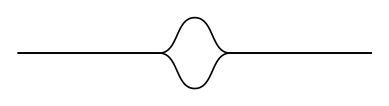
\includegraphics[width=0.10\textwidth]{p147_d1.png}}.
\end{equation}
既然我们只是在做拓扑，就可以稍微松一口气，把它看成圆周上的 $G$-局部系统：
\begin{equation}\tag{10.83}
\Loc_G\!\left(\begin{array}{c}G\\[1pt] \text{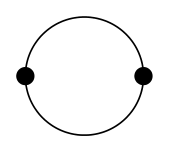
\includegraphics[width=0.05\textwidth]{p147_d2.png}}\\[1pt] G\end{array}\right).
\end{equation}
换句话说，我们看的是圆周上的 $G$-理论，而不是区间上带这些特定边界条件的 $G\times G$-理论。

\begin{srcrem}{55}
这个技巧对一般的 Hecke 代数没有类比。
\end{srcrem}

另一种写法如下。我们考虑 Yang--Mills 理论 $\mathcal{Z}_{G\times G}$，并考虑对角边界条件的自界面：
\diageq{10.84}{0.15\textwidth}{p147_d3.png}
现在我们可以想象把体上的 $G\times G$-理论拆成两份，每一份都标以 $G$-理论：
\begin{equation}\tag{10.85}
\text{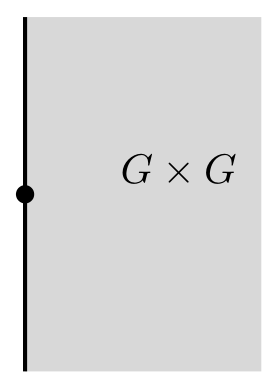
\includegraphics[width=0.10\textwidth]{p148_d1.png}}\;=\;\text{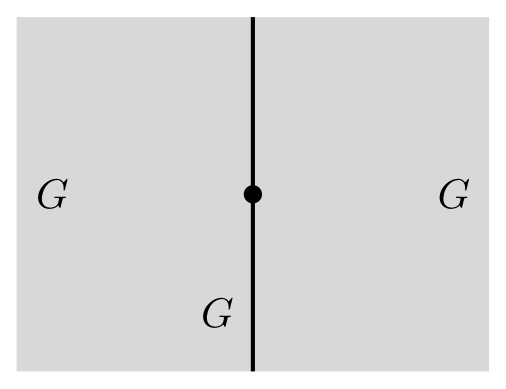
\includegraphics[width=0.17\textwidth]{p148_d2.png}}
\end{equation}
这就是说：$G\times G$-理论的边界条件等同于 $G$-理论的自界面。我们可以把它推广到群的乘积：$G\times H$ 的边界条件等同于 $G$-理论与 $H$-理论之间的界面。

代数上（在足够的对偶性之下），我们这里做的是：
\begin{equation}\tag{10.86}
\Hom(V,W)=V^{*}\otimes W,
\end{equation}
其中左边是界面，右边是乘积理论的边界条件。我们使用的对偶性是 $\C[G]$ 的自对偶性：
\begin{align}
\C[G\times G]\text{-}\mathbf{mod}&=\C[G]\otimes\C[G]\text{-}\mathbf{mod}\tag{10.87}\\
&=\C[G]^{\mathrm{op}}\otimes\C[G]\text{-}\mathbf{mod}\tag{10.88}\\
&=\C[G]\text{-}\mathbf{mod}\text{-}.\tag{10.89}
\end{align}

\begin{srcrem}{56}
这是场论的一个一般事实。一旦理解了边界条件，就理解了界面，反之亦然：场论之间的界面等同于乘积理论的一个边界条件。
\end{srcrem}

\textbf{问题 6.} 为什么 $\mathcal{H}=\mathcal{H}_{G\times G,G}=\C\left[\frac{G}{G}\right]$ 是交换的？

原因是 $\mathcal{H}$ 由 $\mathcal{Z}_G$ 的平凡自界面组成，而后者构成 $\End\big(\mathrm{id}_{\Rep(G)}\big)$。这是 $\Rep(G)$ 的\term{Bernstein 中心}{Bernstein center}。对任意范畴 $\mathcal{C}$，Bernstein 中心是
\begin{equation}\tag{10.90}
\mathcal{Z}(\mathcal{C}):=\End(\mathrm{id}_{\mathcal{C}}).
\end{equation}
断言是：它总是交换的，因为我有两个“方向”来复合这些算子。也就是说，$\mathcal{Z}(\mathcal{C})=\End(\mathrm{id})$ 带有两个相容的幺半结构。一方面，我们可以沿恒等界面碰撞两个界面。另一方面，我们可以把恒等界面的两份自身碰撞，得到：
\begin{equation}\tag{10.91}
\mathrm{id}\circ\mathrm{id}=\mathrm{id}.
\end{equation}
第二种复合对一般的 Hecke 代数没有类比。

\textbf{练习 2.} 带有两个相容幺半结构的集合是交换幺半群。

这是拓扑中 Eckmann--Hilton 论证的玩具版本，后者证明 $\pi_2(X)$ 是交换的。

% [Tutor Note: (10.89) 原文写作“$=\C[G]\text{-}\mathrm{mod}\text{-}$”，末尾的短横线表示右侧还有一个作用未写出，完整写法应为 $\C[G]\text{-}\mathrm{mod}\text{-}\C[G]$（即 $\C[G]$-双模）；这是原文的省略式写法。真正关键的一步是 $\C[G\times G]=\C[G]\otimes\C[G]$ 与 $\C[G]\simeq\C[G]^{\mathrm{op}}$（$g\mapsto g^{-1}$）给出 (10.87)--(10.89) 的链，从而把“乘积理论”翻译成“界面”。]

\begin{srcex}{58}
若 $\mathcal{C}=A\text{-}\mathbf{mod}$，则
\begin{align}
\mathcal{Z}(\mathcal{C})&=\End(\mathrm{id}_{A\text{-}\mathbf{mod}})\tag{10.92}\\
&=\End({}_A A_A),\tag{10.93}
\end{align}
因为如下函子等价：
\begin{equation}\tag{10.94}
(-)\otimes{}_A A_A=\mathrm{id}_{A\text{-}\mathbf{mod}}.
\end{equation}
我们再一次把体上的 $A\otimes A^{\mathrm{op}}$ 理论（边界上带 $A$）“展开”，得到一个体上为 $A$-理论、带平凡界面的理论。但这正好是代数的中心：
\begin{align}
\mathcal{Z}(\mathcal{C})&=\End({}_A A_A)\tag{10.95}\\
&=\mathrm{Z}(A).\tag{10.96}
\end{align}
\end{srcex}

于是对任意范畴 $\mathcal{C}$，我们有一个交换代数 $\mathcal{Z}(\mathcal{C})$。然后我们可以考虑空间：
\begin{equation}\tag{10.97}
\mathcal{M}_{\mathcal{C}}:=\Spec\mathcal{Z}(\mathcal{C}).
\end{equation}
之后我们应当尝试用 $\mathcal{M}_{\mathcal{C}}$ 上的谱分解来理解 $\mathcal{C}$。

\begin{srcex}{59}
若 $\mathcal{C}=A\text{-}\mathbf{mod}$，则我们在 $\Spec\mathrm{Z}(A)$ 上做谱分解。
\end{srcex}

这可能有趣，也可能没有意思，因为中心可能是平凡的。例如在量子力学中，可观测量代数像 Weyl 代数，其中心平凡，于是我们什么也得不到。但断言是：高维 QFT 具有内在的交换性。想法如下。我们考虑体上的理论 $\mathcal{Z}_G$，带一个平凡界面。这等价于理论 $\mathcal{Z}_G$ 有一个 $0$ 维奇点。而这是一个\emph{局部算子}。所以结论是：这种交换性实际上来自局部算子，而不是来自边界条件。

\subsection{物理学中的局部算子}\label{sec:10-5-3}

\term{局部算子}{local operator}是某种局域在时空中一点附近的可观测量。形式上大概是这样的。想法是：在时空中一点的周围，我们考虑半径为 $\epsilon$ 的球面 $S^{n-1}_{\epsilon}$。然后考虑当 $\epsilon\to0$ 时这个球面上的态，它们组成局部算子。所以这类似于该点的一个小去心邻域上场的泛函。注意我们允许在该点处有奇性。

物理学家会告诉你：给定 $x$ 点处的局部算子 $\mathcal{O}_x$，我们可以取期望值：
\begin{equation}\tag{10.98}
\langle\mathcal{O}_x\rangle=\int_{\mathrm{Fields}}\mathcal{O}_x(\varphi)\,e^{-S(\varphi)}\,D\varphi,
\end{equation}
其中我们在 $M\setminus x$ 上对场 $\varphi$ 积分。更一般地，我们有不同点处算子之间的关联函数：
\begin{equation}\tag{10.99}
\big\langle\mathcal{O}_x\mathcal{O}'_y\mathcal{O}''_z\big\rangle=\int \mathcal{O}_x(\varphi)\,\mathcal{O}_y(\varphi)\,\mathcal{O}''_z(\varphi)\,e^{-S(\varphi)}\,D\varphi.
\end{equation}
物理学家还会告诉你的另一件事是\term{算子乘积展开}{operator product expansion}（OPE）：我们尝试取这些点碰撞的极限。于是若从远处看，这些点看起来彼此很近，处于同一个小球内，因此看起来像一个新的复合算子。

在（共形以及）TFT 中，我们有\term{态—算子对应}{state-operator correspondence}：
\begin{equation}\tag{10.100}
\mathcal{Z}\big(S^{n-1}\big)=\text{局部算子的空间},
\end{equation}
其中我们不再需要担心球面的半径。于是 $M\setminus B_{\epsilon}(x)$（即该点某邻域的补）是一个从 $S^{n-1}$ 到 $\varnothing$ 的配边，它给出期望值：
\begin{equation}\tag{10.101}
\langle-\rangle\colon \mathcal{Z}\big(S^{n-1}\big)\longrightarrow\mathcal{Z}(\varnothing_{n-1})=\C.
\end{equation}
所以我们可以直接把局部算子的空间定义为对余维 $1$ 球面的赋值。

\begin{srcex}{60}
考虑有限群 $G$ 的二维 Yang--Mills 理论 $\mathcal{Z}_G$。则局部算子是：
\begin{equation}\tag{10.102}
\mathcal{Z}_G\big(S^1\big)=\C\left[\frac{G}{G}\right].
\end{equation}
对 $\gamma\in\frac{G}{G}$，我们有 delta 函数 $\delta_{\gamma}\in\C\left[\frac{G}{G}\right]$。设 $\Sigma$ 是闭的拓扑曲面。则 $\Sigma\setminus D_x$（即绕该点的一个圆盘的补）是一个配边 $S^1\to\varnothing$。这给出
\begin{equation}\tag{10.103}
\langle-\rangle\colon\C\left[\frac{G}{G}\right]\longrightarrow\C.
\end{equation}
于是
\begin{equation}\tag{10.104}
\langle\delta_{\gamma}\rangle=\#\Loc_G(\Sigma\setminus D,\gamma)
\end{equation}
是绕 $x$ 有单值 $\gamma$ 的 $G$-局部系统的数目。注意这依赖于所处的 Riemann 曲面。
\end{srcex}

关键点是：$\mathcal{H}_{G\times G,G}$ 正好是 $\mathcal{Z}_G$ 中局部算子的代数，而通过画如下图形：
\begin{equation}\tag{10.105}
\text{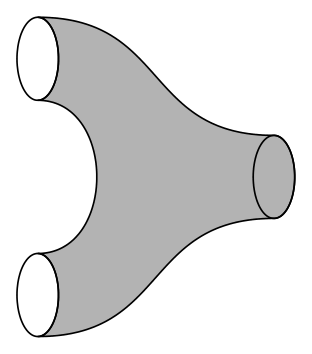
\includegraphics[width=0.12\textwidth]{p150_d1.png}}\;=\;\text{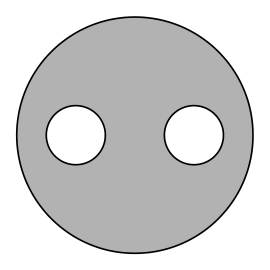
\includegraphics[width=0.11\textwidth]{p150_d2.png}}
\end{equation}
我们得到一个交换的代数结构，因为我们可以让 $x$ 与 $y$ 互相绕行。所以 TFT 中的局部算子（维数 $\ge2$）构成交换代数。

% [Tutor Note: (10.98) 中的积分是形式记号：TFT 中并无真正的测度 $D\varphi$，作者只是借用物理写法来表达“对去心邻域的场求和”。真正严格的表述是 (10.100)--(10.101)：局部算子就是 $\mathcal{Z}(S^{n-1})$，而期望值是从 $S^{n-1}$ 到 $\varnothing$ 的配边所给的线性泛函。另外 (10.104) 的 $\delta_\gamma$ 是共轭类 $\gamma$ 上的 delta 函数，在 $G$ 有限时 $\langle\delta_\gamma\rangle$ 就是一个加权计数，依赖 $\Sigma$ 的拓扑（亏格）。]

\begin{flushright}\small 第 22 讲；2021 年 4 月 15 日\end{flushright}

% ============================================================================
\section{局部算子}\label{sec:10-6}

\begin{sectionkey}
TFT 中的局部算子是 $Z(S^{n-1})$，而把两点处的球面“挤”到一起给出乘法；对 $n\ge2$，$S^{n-1}$ 的链环有足够空间让两点互换，故乘积交换。取谱得到真空模空间，一切东西都成为其上的模——这就是 TFT 的谱分解。
\end{sectionkey}

在\emph{拓扑}场论中，局部算子组成 $\mathcal{Z}\big(S^{n-1}\big)$。

\begin{figure}[htbp]
  \centering
  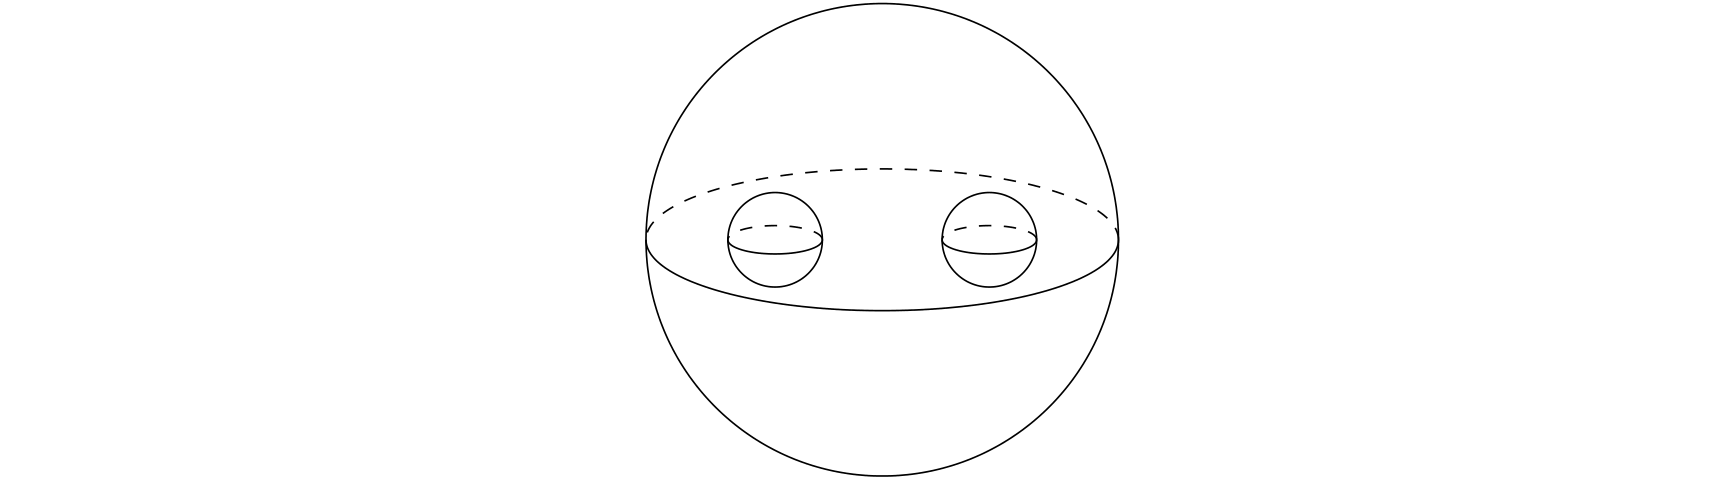
\includegraphics[width=0.30\textwidth]{figure10-3.png}
  \caption{挖去两个小 $3$-球之后的 $3$-球。这是从 $S^2\sqcup S^2$ 到 $S^2$ 的配边。（原文 p.~151，Figure 10.3）}
  \label{fig:10-3}
\end{figure}

% [Tutor Note: 原文 Figure 10.4 只有图题、没有图形（p151 留白），疑为原稿遗漏；本译本照译图题而绝不伪造图形。该图本应画出“挖去三个 $3$-球”的情形，用来看乘积的结合性：中间的球面把两个小球隔开，从而两种“先乘哪一对”的顺序给出同一条配边。下文的 (10.108)--(10.110) 正是这一结合性的二维图示版本。]

\begin{figure}[htbp]
  \centering
  \caption{一个挖去三个 $3$-球的 $3$-球。我们可以把其中两个看成位于某个中间球面之内，这就显示了由图~10.3 所定义的乘积的结合性。（原文 p.~151，Figure 10.4；原缺图形）}
  \label{fig:10-4}
\end{figure}

\subsection{代数结构}\label{sec:10-6-1}

考虑 $n$ 维圆盘 $D^n$ 中的两个点。挖去这两个点的小邻域之后，我们得到图~10.3，它是如下配边：
\begin{equation}\tag{10.106}
S^{n-1}\sqcup S^{n-1}\longrightarrow S^{n-1}.
\end{equation}
TFT $\mathcal{Z}$ 把它送到映射：
\begin{equation}\tag{10.107}
\mathcal{Z}\big(S^{n-1}\big)\otimes\mathcal{Z}\big(S^{n-1}\big)\longrightarrow\mathcal{Z}\big(S^{n-1}\big).
\end{equation}
于是我们得到一族局部算子的乘积，由 $D^n$ 中两个球的位置构型来标记。因为 $\mathcal{Z}$ 是拓扑场论，它在“两点位于 $n$-圆盘中”的构型空间上是局部常值的，所以只依赖于该构型空间的 $\pi_0$。那么这个构型空间的 $\pi_0$ 是什么？

若 $n=1$，则我们考虑的是一个区间内两个（各含一点的、小区间的）点。于是有两种情形：$x$ 在 $y$ 之前，或 $y$ 在 $x$ 之前。所以这个空间不连通，也就是说，我们有两个先验不同的乘积：$\mathcal{O}_x*\mathcal{O}'_y$ 与 $\mathcal{O}'_y*\mathcal{O}_x$。于是我们得到一个结合但未必交换的代数。

（原稿批注：fix fig.\ 10.4——此处待补图~10.4。）事实上，我们在任意维数都能得到结合性。要看到这一点，考虑图~10.4。这个配边是图~10.3 的两份的复合。在二维情形，我们从一个较大的圆盘中挖去两个小圆盘，如图~10.5。

\begin{figure}[htbp]
  \centering
  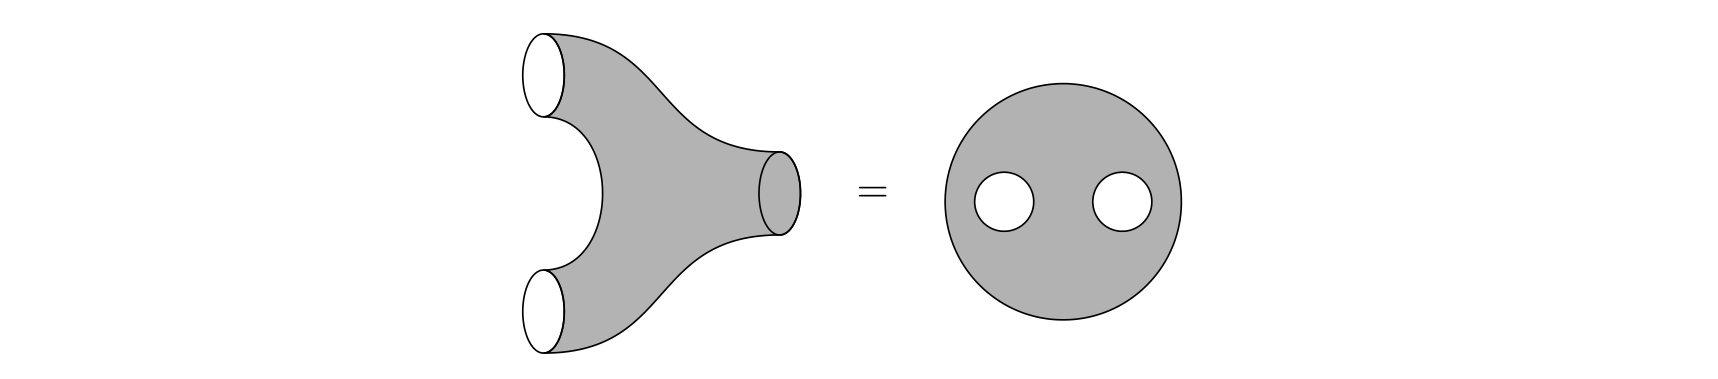
\includegraphics[width=0.34\textwidth]{figure10-5.png}
  \caption{“马裤”配边。这是从 $S^1\sqcup S^1$ 到 $S^1$ 的配边。（原文 p.~152，Figure 10.5）}
  \label{fig:10-5}
\end{figure}

于是复合对应于：
\diagram[0.16\textwidth]{p152_d3.png}
即 (10.108)（上方第一幅：两个“马裤”沿中间的管复合）、(10.109)（中间一幅：它同伦于一个挖去三个小圆盘的圆盘）与 (10.110)（下方一幅：它又同伦于先右后左的另一种复合），这就证明了结合性。
\begin{equation}\tag{10.108}
\text{两副“马裤”沿中间管道复合}
\end{equation}
\begin{equation}\tag{10.109}
\text{同伦于：一个圆盘挖去三个小圆盘}
\end{equation}
\begin{equation}\tag{10.110}
\text{又同伦于：交换左右顺序后的复合}
\end{equation}
若 $n>1$，则圆盘中一对圆盘（或同伦地，一对点）的构型空间是连通的。这告诉我们：
\begin{equation}\tag{10.111}
\big(\mathcal{Z}(S^{n-1}),\,*\big)
\end{equation}
是一个交换代数。

\begin{srcrem}{57}
这是拓扑量子场论的一个关键特征。量子力学本质上不交换，但一旦进入更高维数，我们就有了这种交换性。
\end{srcrem}

% [Tutor Note: 结合性的两张图不要“从字面上”看混：(10.108) 是“先粘左边一对、再粘第三个”，(10.110) 是“先粘右边一对、再粘第一个”，两者都同伦于 (10.109)（一个圆盘挖去三个小圆盘），所以乘积结合。交换性则是另一回事：它需要两点在构型空间中可以互换，这只有当 $n\ge2$（此时 $\pi_0$ 为单点，甚至 $n\ge3$ 时基本群平凡）才成立。]

\subsection{谱分解}\label{sec:10-6-2}

正如我们已经看到的，一般原则是：如果有人递给你一个交换代数，你就应当取它的 $\Spec$。于是给定 $n$ 维 TFT（$n>1$），我们可以定义一个仿射簇：
\begin{equation}\tag{10.112}
\mathcal{M}_{\mathcal{Z}}^{0}:=\Spec\Big(\mathcal{Z}\big(S^{n-1}\big),\,*\Big).
\end{equation}
这称为\term{真空模空间}{moduli space of vacua}，即这个空间的一点是场论的一个\term{真空}{vacuum}。真空是定义配分函数、期望值等所需数据的一部分。例如，对定义在 $\R^{n}$ 上的量子场论，我们可能尝试定义 $\R^{n}$ 上的配分函数，但由于 $\R^{n}$ 非紧，它不会被良好定义。所以我们需要在无穷远处固定一些数据，也就是在无穷远处紧化；而我们这里看到的是 $\mathcal{Z}\big(S^{n-1}\big)$ 的一个元素。

\begin{srcrem}{58}
我们最初是通过看非常靠近一点的算子（例如在\emph{紫外}）而遇见 $\mathcal{Z}\big(S^{n-1}\big)$ 的。现在我们看到 $\mathcal{Z}\big(S^{n-1}\big)$ 通过看非常远的地方（即在无穷远）而出现。这两者一致，因为\emph{拓扑}量子场论不知道大球面与小球面的区别。换句话说，对拓扑场论，紫外与红外变得相同。在通常的量子场论中，真空与局部算子之间的联系没有这么直接。
\end{srcrem}

给定局部算子 $\mathcal{O}$ 与真空 $\langle0\rangle$，我们可以定义 $\mathcal{O}$ 的真空期望值，即某个数，写作 $\langle0|\mathcal{O}|0\rangle$。所以我们只需把真空看成为使这些期望值有良好定义而需要选择的东西。也就是说，算子给出真空空间上的函数。在 TFT 的框架里，我们将用这一点作为真空的\emph{定义}：真空是 $\Spec\mathcal{Z}\big(S^{n-1}\big)$ 中的一点。

要点是：TFT 同义反复地在其模空间 $\mathcal{M}_{\mathcal{Z}}^{0}$ 上谱分解。也就是说，TFT 中的一切都是 $\mathcal{Z}\big(S^{n-1}\big)$ 上的线性对象。

这是一个代数，所以它当然作用于自身；但周围还有许多其他自然的模。设 $M$ 是 $(n-1)$-流形。那么断言是：$\mathcal{Z}(M)$ 是 $\mathcal{Z}\big(S^{n-1}\big)$ 上的模。考虑配边 $M\times I$，它诱导 $\mathcal{Z}(M)$ 上的恒等映射。然后在区间的某一点处，我们可以认为插入了一个算子，即在该点周围挖去一个小球，得到图~10.6。所得的流形 $(M\times I)\setminus D_x$ 是一个（原稿批注：redo figure——此图待重画）配边：
\begin{equation}\tag{10.113}
M\sqcup S^{n-1}\longrightarrow M,
\end{equation}
它诱导映射：
\begin{equation}\tag{10.114}
\mathrm{act}_x\colon \mathcal{Z}(M)\otimes\mathcal{Z}\big(S^{n-1}\big)\longrightarrow\mathcal{Z}(M).
\end{equation}
这个映射通过画与图~10.4 类似的图把 $\mathcal{Z}(M)$ 实现为模。因此我们可以把 $\mathcal{Z}(M)$ 看成模空间上的层：
\begin{equation}\tag{10.115}
\mathcal{Z}(M)\in \QC\big(\mathcal{M}_{\mathcal{Z}}^{0}\big)=\mathcal{Z}\big(S^{n-1}\big)\text{-}\mathbf{mod}.
\end{equation}

\begin{figure}[htbp]
  \centering
  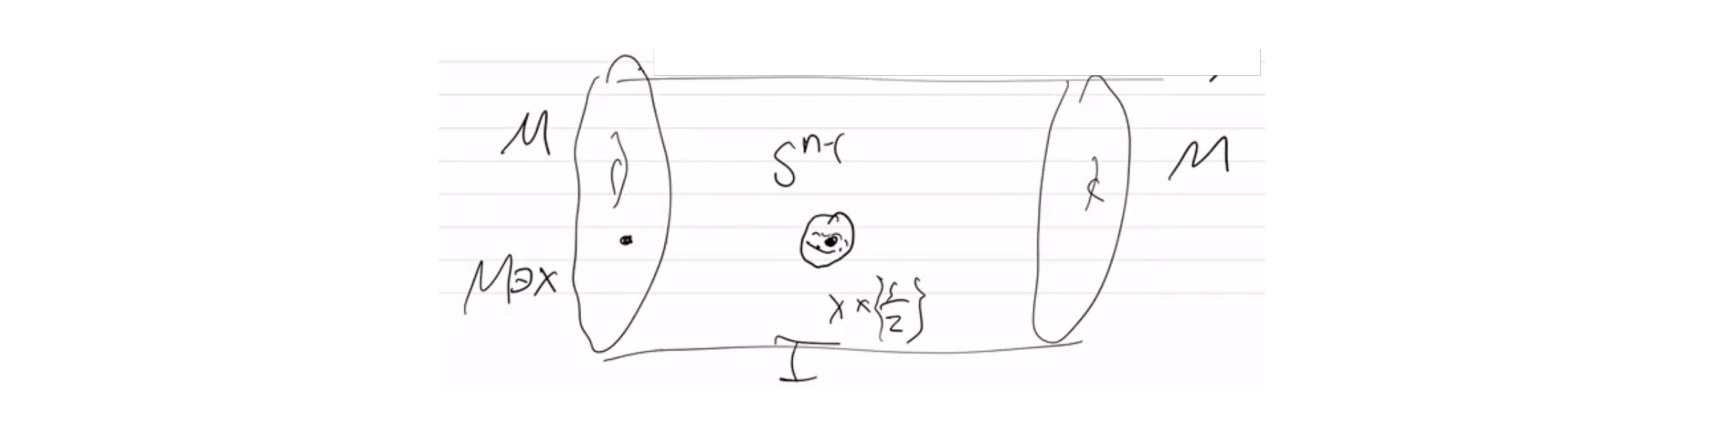
\includegraphics[width=0.55\textwidth]{figure10-6.png}
  \caption{从 $M^{n-1}\times I$ 中挖去一个小球，得到从 $M^{n-1}\sqcup S^{n-1}$ 到 $M^{n-1}$ 的配边。这诱导出 $\mathcal{Z}\big(M^{n-1}\big)$ 上的模结构。（原文 p.~154，Figure 10.6）}
  \label{fig:10-6}
\end{figure}

\begin{srcrem}{59}
对每一点 $x\in M$，我们都有 $\mathcal{Z}\big(S^{n-1}\big)$ 在 $\mathcal{Z}(M)$ 上的作用。于是这个巨大的张量积 $\otimes_{x\in M}\mathcal{Z}\big(S^{n-1}\big)$ 作用在 $\mathcal{Z}(M)$ 上，但实际上它通过所谓的\term{因子化同调}{factorization homology}分解：
\begin{equation}\tag{10.116}
\int_{M}\mathcal{Z}\big(S^{n-1}\big),
\end{equation}
它由从 $M$ 到真空模空间的局部常值映射上的函数组成：
\begin{equation}\tag{10.117}
\mathcal{O}\big(\mathrm{Map}_{\mathrm{l.c.}}(M,\mathcal{M}_{\mathcal{Z}})\big).
\end{equation}
\end{srcrem}

% [Tutor Note: (10.112) 的 $\Spec$ 里是交换代数 $(\mathcal{Z}(S^{n-1}),*)$，而不是某个向量空间；$\mathcal{M}_{\mathcal{Z}}^{0}$ 是“真空模空间”，它未必光滑、未必约化。(10.116) 的因子化同调 $\int_M$ 不是普通积分，而是把每一点的局部算子代数沿着 $M$ 装配起来的余极限；当 $M$ 连通时它常退化为 $\mathcal{Z}(S^{n-1})$，这正是 (10.115) 中 $\QC(\mathcal{M}^0_{\mathcal{Z}})=\mathcal{Z}(S^{n-1})\text{-}\mathbf{mod}$ 的来源。]

\subsection{二维 TFT}\label{sec:10-6-3}

局部算子组成态空间 $\mathcal{Z}\big(S^1\big)$。上一次我们研究它时，考虑的是 $\mathcal{Z}$ 与自身之间的恒等界面，然后取 $\End(\mathrm{id}_{\mathcal{C}})$（其中 $\mathcal{C}$ 是边界条件的范畴）。回忆这是 Bernstein 中心
\begin{equation}\tag{10.118}
\End(\mathrm{id}_{\mathcal{C}})=\mathcal{Z}(\mathcal{C}).
\end{equation}
所以这与 $\mathcal{Z}\big(S^1\big)$ 相同。若 $\mathcal{Z}=\mathcal{Z}_G$ 是有限群 $G$ 的二维 Yang--Mills 理论，则
\begin{equation}\tag{10.119}
\mathcal{Z}_G\big(S^1\big)=\C\left[\frac{G}{G}\right]
\end{equation}
（带卷积）是群代数 $\C G$ 的中心。

真空模空间是：
\begin{align}
\mathcal{M}_{\mathcal{Z}_G}^{0}&=\Spec\mathcal{Z}_G\big(S^1\big)\tag{10.120}\\
&=\Spec\C\left[\frac{G}{G}\right]\tag{10.121}\\
&=:\widehat{G},\tag{10.122}
\end{align}
我们将称之为群 $G$ 的\term{酉对偶}{unitary dual}。断言是：$\widehat{G}$ 是 $G$ 的不可约表示的等价类的集合。有限群的表示由 Maschke 定理分解为不可约表示：
\begin{equation}\tag{10.123}
\Rep(G)\simeq\bigoplus_{\text{不可约表示 }V_\lambda\text{ 的等价类}}(\Vect)\otimes V_\lambda.
\end{equation}
也就是说，任何表示可以写成：
\begin{equation}\tag{10.124}
V\simeq\bigoplus_{\lambda\in\widehat{G}}V_\lambda^{\oplus m_\lambda}.
\end{equation}
换言之：
\begin{equation}\tag{10.125}
\Rep(G)\simeq\Vect\big(\widehat{G}\big)=\QC\big(\widehat{G}\big).
\end{equation}
这是谱分解的一个版本。

我们说 $\mathcal{Z}\big(M^{n-1}\big)$ 是 $\mathcal{Z}\big(S^{n-1}\big)$ 上的模。但在二维情形我们得不到太多东西，因为没有多少紧的 $1$-流形。不过我们确实有有意思的带边界的 $1$-流形，例如
\begin{equation}\tag{10.126}
\textcolor{red}{\bullet}\!\!-\!\!-\!\!-\!\!-\!\!\textcolor{blue}{\bullet},
\end{equation}
其中 $V,W\in\Rep(G)$。然后我们有从这个流形到自身、并挖去一个小圆盘的配边：
\diageq{10.127}{0.17\textwidth}{p155_d1.png}
因此 $\mathcal{Z}\big(S^1\big)$ 作用在：
\begin{equation}\tag{10.128}
\mathcal{Z}\big(S^1\big)\curvearrowright
\mathcal{Z}\Big(\textcolor{red}{\bullet}\!\!-\!\!-\!\!-\!\!-\!\!\textcolor{blue}{\bullet}\Big)
=\Hom(V,W)
\end{equation}
也就是说，范畴 $\Rep(G)$ 在 $\mathcal{Z}\big(S^1\big)$-模中富化。等价地，这是一个 $\mathcal{Z}\big(S^1\big)$-线性范畴。

这并不是有限群理论的特例。在任意二维 TFT 中，边界条件的范畴 $\mathcal{C}$ 都是 $\mathcal{Z}\big(S^1\big)=\mathcal{Z}(\mathcal{C})$-线性的。事实上任意范畴 $\mathcal{C}$ 都在 $\mathcal{Z}(\mathcal{C})=\End(\mathrm{id})$ 上线性。这是使 $\mathcal{C}$ 线性的泛代数。也就是说，$\mathcal{C}$ 中的 $\Hom$ 空间自然地落在 $\QC(\Spec\mathcal{Z}(\mathcal{C}))$ 中。想法是：$\mathcal{C}$ 构成 $\mathcal{M}=\Spec\mathcal{Z}(\mathcal{C})$ 上的范畴层。这意味着 $\Hom$ 空间被升级为该空间上的层，即它们是 $\mathcal{Z}(\mathcal{C})$ 上的模。

一般地，我们可以说 $\mathcal{C}$ 是 $R$-线性的，如果 $\Hom$ 空间是 $R$-模，或者等价地，如果存在映射 $R\to\mathcal{Z}(\mathcal{C})$。如果我们处于“大”的设定，即 $\mathcal{C}$ 有足够多的余极限（余完备），那么这等价于说 $\mathcal{C}$ 是 $R\text{-}\mathbf{mod}$ 上的模范畴。

于是我们有三个不同的想法，我们希望把它们内化为同一件事：
\begin{enumerate}
\item $\mathcal{C}$ 构成（拟凝聚的）范畴层；
\item $\mathcal{C}$ 是 $R$-线性的，即存在映射 $R\to\mathcal{Z}(\mathcal{C})$；
\item $\mathcal{C}$ 是 $R\text{-}\mathbf{mod}$ 上的模范畴。
\end{enumerate}
也就是说：$\mathcal{C}$ 是 $\Spec R$ 上的（拟凝聚）范畴层，等价于存在映射 $R\to\mathcal{Z}(\mathcal{C})$，等价于 $\mathcal{C}$ 在 $R$-模中富化，这又说明 $\mathcal{C}$ 带有 $(\mathbf{mod}\text{-}R,\otimes_R)$ 的作用。最后这个刻画看起来有点不同。为了对 $M\in R\text{-}\mathbf{mod}$ 与 $C\in\mathcal{C}$ 定义 $M\otimes C$ 之类的东西，我们先把 $M$ 消解为自由模的复形：
\begin{equation}\tag{10.129}
\cdots\longrightarrow R^{\oplus n_2}\longrightarrow R^{\oplus n_1}\longrightarrow M,
\end{equation}
其中映射是元素在 $R$ 中的矩阵。我们知道 $\mathcal{C}$ 与自由模 $R^{\oplus n_1}$ 的张量积就是 $\mathcal{C}^{\oplus n_1}$。由于范畴是 $R$-线性的，我们可以把这些同样的矩阵写成如下对象之间的映射：
\begin{equation}\tag{10.130}
\cdots\longrightarrow \mathcal{C}^{\oplus n_2}\longrightarrow \mathcal{C}^{\oplus n_1},
\end{equation}
而这是 $M\otimes C$ 的一个消解。这里正是我们用到余极限假设的地方：我们需要写下这些消解并在最后取其余极限。例如群/结合代数的模满足这一点。

\paragraph{局部化}

若 $\mathcal{C}$ 是 $R\text{-}\mathbf{mod}$ 上的模，我们可以在 $\Spec R$ 上定义它的局部化。回忆对通常的模，我们把 $M$ 关于 $R$ 的局部化定义为：
\begin{equation}\tag{10.131}
\underline{M}(U)=M\otimes_R\mathcal{O}(U),
\end{equation}
其中 $U\subset\Spec R$ 是开集。要点是：$\mathcal{O}(U)=R[S^{-1}]$（对某个乘性子集 $S$），于是 $\underline{M}(U)=M[S^{-1}]$。这给出 $R\text{-}\mathbf{mod}$ 与 $\Spec R$ 上拟凝聚层之间的范畴等价。

在范畴的设定下同样的图像也适用。设 $\mathcal{C}\curvearrowright R\text{-}\mathbf{mod}$，于是我们可以构造：
\begin{equation}\tag{10.132}
\underline{\mathcal{C}}(U)=\mathcal{C}\otimes_{R\text{-}\mathbf{mod}}R[S^{-1}]\text{-}\mathbf{mod},
\end{equation}
其中 $U=\Spec R[S^{-1}]$。这就是把 $\mathcal{C}$ 中所有来自 $S\subset R$ 的态射求逆所得的范畴。

对结合代数 $A$（例如 $\C G$），$A\text{-}\mathbf{mod}$ 在 $\Spec\mathcal{Z}(A)$ 上成层。类似地，$\Rep(G)$ 在 $\widehat{G}$ 上成层；而我们可以把表示分解为不可约表示这一事实给出：
\begin{equation}\tag{10.133}
\Rep(G)\simeq\QC\big(\widehat{G}\big).
\end{equation}
这听起来像某种 Fourier 变换的版本，但它并不是典范的。这幅图像里有点可疑之处。同义反复地为真的事情是：$\Rep(G)$ 在中心上成层。给定 $\widehat{G}$ 的任意子集 $S$，我们可以构造 $\Rep(G)$ 的一个直和项，由所有特征落在 $S$ 中的表示组成。但为了得到 $\Rep(G)$ 与 $\Vect^{\widehat{G}}$ 之间的等同，我们需要选取同构类的代表元。另一种办法是，Wedderburn 定理（有限群的 Peter--Weyl 定理）告诉我们：
\begin{equation}\tag{10.134}
\C G\simeq\bigoplus_{V_\lambda\ \text{不可约}}\End(V_\lambda),
\end{equation}
其中 $\End(V_\lambda)=M_{n_\lambda\times n_\lambda}(\C)$，而 $n_\lambda=\dim V_\lambda$。也就是说，$\C G$ 分解为 $\widehat{G}$ 上若干个结合代数的直和，而这些结合代数原来是除代数上的矩阵代数。

这可不是小问题。如果记录“实性”，即考虑实表示，这个同构就不再成立。于是我们考虑 $G$ 的实表示，并看不可约特征的集合 $\widehat{G}$，它带有自然的实结构。不可约表示 $V$ 有三种类型。Schur 引理告诉我们，我们得到 $\R$ 的某个扩域上的除代数：
\begin{equation}\tag{10.135}
\End(V)=\begin{cases}\R\\ \C\\ \HH\end{cases}.
\end{equation}
$\R$ 与 $\HH$ 对应于对偶的实点：$\widehat{G}_{\R}$。复的情形意味着对偶中有复共轭成对的点，即特征不是实值的。但即使特征实值，$\End(V)$ 也不一定是 $\R$，而只是 $\R$ 上的某个除代数。这告诉我们：Wedderburn 分解并不给出 $V$ 的自同态，我们得到的是这个四元数版本。于是 $\QC\big(\widehat{G}\big)$ 作为可逆模范畴非平凡地作用在 $\Rep_{\R}(G)$ 上。也就是说，$\Rep_{\R}(G)$ 是一个范畴化的线丛（$\QC\big(\widehat{G}\big)$ 的可逆模），即一个\term{Gerbe}{Gerbe}。这些对应于 Brauer 群的元素（例如四元数 $\HH$ 在 $\R$ 的 Brauer 群中）。这个 gerbe 与物理学中所谓的\term{反常}{anomaly}有关。

同义反复地为真的是：$\mathcal{C}$ 在 $\mathcal{M}$ 上成层。最简单的答案就是它恰为 $\QC(\mathcal{M})$ 本身。下一个最复杂的情形是 gerbe（$\QC$ 的反常或扭转版本），或者还可能更复杂。

对二维 TFT $\mathcal{Z}$，我们附上局部算子的交换环 $\mathcal{Z}\big(S^1\big)$，它是 $\mathcal{Z}$ 中可观测量代数的一个版本；我们通过用这些算子作用来做观测。于是我们发现 $\mathcal{Z}$ 在 $\mathcal{M}_{\mathcal{Z}}$ 上成层。

\begin{srcrem}{60}
Mednykh 公式告诉我们：
\begin{align}
\mathcal{Z}_G\big(\Sigma^{g}\big)&=\#\Loc_G\Sigma^{g}\tag{10.136}\\
&=\sum_{\chi\in\widehat{G}}\left(\frac{|G|}{\dim(V_\chi)}\right)^{2g-2}.\tag{10.137}
\end{align}
\end{srcrem}

\begin{flushright}\small（原稿批注：transition。）\end{flushright}

\begin{flushright}\small 第 23 讲；2021 年 4 月 20 日\end{flushright}

到目前为止我们已经看到：
\begin{itemize}
\item $\mathcal{Z}\big(S^{n-1}\big)$（局部算子的空间）对 $n\ge2$ 构成交换环；
\item $\mathcal{Z}\big(M^{n-1}\big)$ 自然地是 $\mathcal{Z}\big(S^{n-1}\big)$ 上的模；
\item $\mathcal{Z}\big(N^{n-2}\big)$ 自然地在 $\mathcal{Z}\big(S^{n-1}\big)$ 上线性。
\end{itemize}
我们只对二维 TFT 看到了最后一点，但它在一般情形也成立。要看到这一点，考虑从 $N^{n-2}\times I$ 到自身的恒等配边，即 $(N^{n-2}\times I)\times I$。然后我们挖去一个小圆盘，得到如下配边：
\diageq{10.138}{0.17\textwidth}{p157_d2.png}
这里我们把那个点看成 $N^{n-2}$，也就是说，我们暗中把整幅图与 $N^{n-2}$ 作乘积。于是我们有
\begin{equation}\tag{10.139}
\mathcal{Z}\big(\textcolor{red}{\bullet}\!\!-\!\!-\!\!-\!\!\textcolor{blue}{\bullet}\big),
\end{equation}
它是 $\mathcal{Z}\big(N^{n-2}\big)$ 中的一个 $\Hom$-空间，实际上是交换环 $\mathcal{Z}\big(S^{n-1}\big)$ 上的模。

然后我们发现，可以用如下簇来组织这个结构：
\begin{equation}\tag{10.140}
\mathcal{M}_{\mathcal{Z}}^{\mathrm{aff}}=\mathcal{M}_{\mathcal{Z}}^{0}:=\Spec\mathcal{Z}\big(S^{n-1}\big),
\end{equation}
称为真空模空间。想法是：我们可以把任意的理论 $\mathcal{Z}$ 与一个拉格朗日场论联系起来，后者的场空间是映入 $\mathcal{M}_{\mathcal{Z}}^{0}$ 的映射空间。这些就是我们将在下一节定义的 B-模型。

\begin{srcex}{61}
若 $\mathcal{Z}_G$ 是有限群 $G$ 的二维 Yang--Mills 理论，则 $\mathcal{M}_{\mathcal{Z}}^{0}=\widehat{G}$，这就给出 $\mathcal{Z}$ 分解为不可约部分。
\end{srcex}

% [Tutor Note: (10.136) 左边原文印作 $\mathcal{Z}_G(\Sigma^{G})$，上标是大写 $G$，按意义应为亏格 $g$（右边写的是 $\Sigma^{g}$ 与 $2g-2$），这是原稿的笔误，照译并指出。另外“$\Rep(G)$ 在 $\widehat{G}$ 上成层”并不是典范的：如作者所述，要把它变成真正的 $\QC(\widehat{G})$，需要选代表元；实表示的情形只能得到 gerbe，这正是物理上“反常”的几何来源。]

% ============================================================================
\section{B-模型}\label{sec:10-7}

\begin{sectionkey}
对任意交换环 $R$，用“局部常值映射”构造截断的 B-模型：$(n-1)$-流形给函数环、$(n-2)$-流形给模范畴，推拉由对应给出。于是任一 TFT 都能与它的谱上的 B-模型比较，谱分解就是说“理论是高一维 B-模型的边界条件”。
\end{sectionkey}

设 $R$ 是交换环（等价地，可以想成簇 $X=\Spec R$）。由它我们可以构造任意维数的（截断）TFT。这里“截断”的意思是：我们不去关心给最高维配边附上数。这是一个拉格朗日场论，所以对流形 $M$ 我们有场的概念，由下式给出：
\begin{equation}\tag{10.141}
\mathrm{Map}(M,\Spec R=X).
\end{equation}
我们如何让光滑流形与仿射簇之间产生有趣的相互作用？我们将考虑它们之间能考虑的“最笨”的相互作用：局部常值映射。也就是说，我们考虑：
\begin{equation}\tag{10.142}
\mathrm{Map}_{\mathrm{lc}}(M,X)=\mathrm{Map}(\pi_0(M),X).
\end{equation}
用环的语言，这就是：
\begin{equation}\tag{10.143}
\mathrm{Map}_{\mathrm{lc}}(M,X)=\Spec\big(R\otimes\pi_0(M)\big).
\end{equation}
然后我们可以如下定义 $X=\Spec R$ 上的（截断）$n$ 维 B-模型。对 $(n-1)$-流形我们赋予：
\begin{equation}\tag{10.144}
B_X^{n}\big(M^{n-1}\big)=\mathcal{O}\big(\mathrm{Map}(M,X)\big)=R\otimes\pi_0(M).
\end{equation}
对 $(n-2)$-流形我们赋予：
\begin{equation}\tag{10.145}
B_X^{n}\big(N^{n-2}\big)=\QC\big(\mathrm{Map}(N,X)\big)=\big(R\otimes\pi_0(N)\big)\text{-}\mathbf{mod}.
\end{equation}
然后可以由如下对应（span，即双拉回图）定义你想要的任何推拉运算：
\begin{equation}\tag{10.146}
\begin{array}{ccc}
& \mathrm{Map}(M,X) &\\[4pt]
\swarrow & & \searrow\\[4pt]
\mathrm{Map}(\partial_{\mathrm{in}},X) & & \mathrm{Map}(\partial_{\mathrm{out}},X)
\end{array}
\end{equation}

这与谱分解有什么关系？我们从一个 $n$ 维 TFT $\mathcal{Z}$ 出发，然后构造了这个环 $\big(\mathcal{Z}(S^{n-1}),*\big)$，并由它定义 B-模型
\begin{equation}\tag{10.147}
B_{\mathcal{M}_{\mathcal{Z}}^{0}}^{n}.
\end{equation}
朴素的想法是：$\mathcal{Z}$ 看起来像理论 $B_{\mathcal{M}_{\mathcal{Z}}^{0}}^{n}$。

\begin{srcex}{62}
考虑有限群 $G$ 的二维 Yang--Mills 理论 $\mathcal{Z}_G$。则 $\mathcal{M}_{\mathcal{Z}}^{0}=\widehat{G}$，
\begin{equation}\tag{10.148}
\mathcal{Z}_G\big(S^1\big)=\C\left[\frac{G}{G}\right]\simeq\C\big[\widehat{G}\big]
\end{equation}
是局部算子的环，而
\begin{equation}\tag{10.149}
\mathcal{Z}_G(\mathrm{pt})=\Rep(G)\simeq\QC\big(\widehat{G}\big),
\end{equation}
它也是 $B_{\mathcal{M}_{\mathcal{Z}}^{0}}^{2}(\mathrm{pt})$。也就是说，我们只看这个类函数环就能重建理论。
\end{srcex}

\begin{srcrem}{61}
镜像对称正是这类想法。事实上，Gross--Siebert 的“内蕴镜像对称”就是紧密仿照这个想法构造的。从一个有意思的理论出发（原稿批注：cite——此处需补文献），即引用辛拓扑中的 A-模型；然后构造一个簇（镜像），作为局部算子环的谱。接着镜像对称说：你出发时的 A-模型与你所构造的 B-模型是等价的。
\end{srcrem}

即使对有限群 $G$，$\Rep_{\R}G$ 也不会恰好等于朴素的答案 $\QC\big(\widehat{G}\big)$。

相反，靠抽象废话，我们得到如下结果。我们知道 $\mathcal{Z}\big(M^{n-1}\big)$ 是 $\mathcal{Z}\big(S^{n-1}\big)$ 上的模。我们通过与区间作乘积并插入一个局部算子而得到这个结构，也就是如图~10.6 那样挖去一个小球。所以实际上，对 $M$ 中每一点我们都得到一个模结构族，使得当我们沿两点之间的路径走时，相应的作用被等同起来。也就是说，它局部常值地依赖于 $x\in M$。于是我们自然得到：$\mathcal{Z}(M)$ 是 $\mathcal{Z}\big(S^{n-1}\big)$ 的 $\pi_0(M)$ 多份拷贝上的模，即如下作用：
\begin{equation}\tag{10.150}
\pi_0(M)\otimes\mathcal{Z}\big(S^{n-1}\big)=\mathcal{O}\big(\mathrm{Map}(M,\mathcal{M}_{\mathcal{Z}}^{0})\big).
\end{equation}
所以我们并没有得到这个向量空间与这个环之间的同构，而是得到：$\mathcal{Z}(M)$ 是 $\mathcal{O}\big(\mathrm{Map}(M,\mathcal{M}_{\mathcal{Z}}^{0})\big)$ 上的模，即它是一个对象：
\begin{equation}\tag{10.151}
\mathcal{Z}(M)\in \QC\big(\mathcal{M}_{\mathcal{Z}}^{0}\big),
\end{equation}
也就是说
\begin{equation}\tag{10.152}
\mathcal{Z}(M)\in B_{\mathcal{M}_{\mathcal{Z}}^{0}}^{n+1}(M).
\end{equation}
同样，$\mathcal{Z}(N)$ 是 $R$-线性范畴，但实际上它可以细化为一个在 $\pi_0(N)\otimes R$ 上线性的范畴，即
\begin{equation}\tag{10.153}
\mathcal{Z}(N)\in B_{\mathcal{M}_{\mathcal{Z}}^{0}}^{n+1}(N)=\text{$\mathcal{M}_{\mathcal{Z}}^{0}$ 上的范畴层 $2$-范畴}.
\end{equation}

总结一下：场论的谱分解是这样说的。我们从 $n$ 维 TFT $\mathcal{Z}$（即我们的态）出发。然后我们有可观测对象（局部算子），它们作用在态上。我们可以把它重新表述为：
\begin{equation}\tag{10.154}
\mathcal{Z}(-)\in B_{\mathcal{M}_{\mathcal{Z}}^{0}}^{n+1}(-).
\end{equation}
等价地说，理论 $\mathcal{Z}$ 是这个高一维的 B-模 $B_{\mathcal{M}_{\mathcal{Z}}^{0}}^{n+1}$ 的边界条件。也就是说，我们把 $M\times I$ 带一个红色（标以 $\mathcal{Z}$ 的）边界：
\diageq{10.155}{0.15\textwidth}{p159_d2.png}
我们最初把边界条件想成群表示，或一般地，想成范畴的对象。我们这里所做的只是同一想法的更精致版本。

回忆我们当时正走向这些四维 A-模型。我们只讨论了群 $G=\mathrm{GL}_1$ 的情形，其中我们得到拓扑 Maxwell 理论 $\mathcal{A}_{\mathrm{GL}_1}$。这个理论赋予三维流形 $M^3$ 的向量空间 $\mathcal{A}_{\mathrm{GL}_1}(M^3)$，是 $\mathrm{Pic}(M^3)$ 上的局部常值函数。回忆 $\mathrm{Pic}(M^3)$ 是 $U(1)$-联络模规范等价的空间。现在我们可以问局部算子是什么，并尝试像上面那样玩谱分解的游戏。

回忆 $\mathrm{Pic}(M)$ 看起来像格 $H^2(M,\Z)$ 与一个环面的交叉，后者有 $\pi_1=H^1(M,\Z)$。局部算子将来自对 $S^3$ 的赋值，但 $S^3$ 既没有 $H^2$ 也没有 $H^1$，所以我们得到
\begin{equation}\tag{10.156}
\mathrm{Pic}\big(S^3\big)=\mathrm{pt}.
\end{equation}
如果我们对自同构小心一点，这里可能得到 $BU(1)$ 之类的东西。无论如何，其上的局部常值函数是平凡的，所以我们没有任何局部算子。在导出版本中我们会得到：
\begin{equation}\tag{10.157}
H^{*}\big(BU(1)\big)=\C[u],
\end{equation}
但这仍然不太有意思/有用。

% [Tutor Note: 本节要抓住“比较”的逻辑：任给交换环 $R$ 都有截断 B-模型 $B^n_X$（局部常值映射），它是“最简单的拉格朗日理论”；对任意 TFT $\mathcal{Z}$，用它的局部算子环造出 $B^{n+1}_{\mathcal{M}^0_{\mathcal{Z}}}$，谱分解的准确内容就是 (10.152)--(10.154)：$\mathcal{Z}$ 是该 B-模型的边界条件，而不是说 $\mathcal{Z}$ 与它相等。$R\otimes\pi_0(M)$ 是“每个连通分支一份 $R$”的简写，不要理解成真的张量积。]

% ============================================================================
\section{缺陷}\label{sec:10-8}

\begin{sectionkey}
把“标记点”换成“嵌入子流形”，局部算子的故事就推广为缺陷：余维 $k$ 缺陷由 $Z(S^{k-1})$ 标记。线算子（$k=2$）随维数升高依次得到 $E_1$、$E_2$、$E_\infty$ 结构；四维时线算子的谱给出 $\mathcal{M}^1_Z$，它是 $\mathcal{M}^0_Z$ 的仿射化。
\end{sectionkey}

现在我们要把关于局部算子的故事推广到线算子。为此我们将引入一般的缺陷算子，而这又需要讨论配边假设。

\subsection{配边假设}\label{sec:10-8-1}

（原稿批注：fix and cite——此处需补文献。）配边假设由 Baez--Dolan 提出，并由 Hopkins--Lurie、Lurie、Ayala--Francis、Schommer--Pries 证明。配边假设是拓扑场论中的某些概念与范畴论中的某些概念之间的等价。我们将把它看成从范畴数据构造拓扑场论的方法。也可以反过来看，即把它看成对“为什么各种图示演算能描述范畴论”的解释：它告诉我们，可以画图而不必去想范畴。

\term{扩展拓扑场论}{extended topological field theory}是配边范畴的一个表示，即一个对称幺半函子：
\begin{equation}\tag{10.158}
\mathcal{Z}\colon\big(\Bord_n^{\square},\sqcup\big)\longrightarrow\big(\mathcal{C},\otimes\big),
\end{equation}
其中 $\square$ 可以是任意选定的\term{切向结构}{tangential structure}。例如，我们可能要求配边是定向的、标架的，或一般地具有 $G$-结构（只要有一个映射 $G\to O(n)$）。若 $G=1$，则 $G$-结构就是 $n$-标架。若 $G=SO(n)$，则 $G$-结构等价于在 $M$ 上选取一个定向。若 $G=O(n)$，则 $M$ 上的 $G$-结构不包含任何额外结构。无论如何，要画的基本图像是：这个范畴中的流形总带有 $n$ 维切丛。也就是说，与一个点不同，我们可以画一小块 $\R^n$。

配边假设说：场论 $\mathcal{Z}$ 的结构完全由数据 $\mathcal{Z}(\mathrm{pt})\in\mathcal{C}$ 决定，但要服从：
\begin{itemize}
\item 可对偶性（有限性条件）；
\item 自对偶结构（这依赖于 $\square$）。
\end{itemize}
对一维理论，可对偶性问的是赋予点的向量空间是否有对偶。自对偶约束与切向结构的选择有关。

\subsection{带奇点的配边假设}\label{sec:10-8-2}

（原稿批注：Cite——此处需补文献。）这出现在 Lurie 的工作中，是 Baez--Dolan 的一个猜想（称为\emph{tangle 猜想}）的推广。我们把配边假设描述为拓扑场论与范畴论之间的某种等价。到目前为止，配边假设的陈述只告诉我们对象层面的等价，并没有反映我们在范畴论中看到的某些图示结构，例如态射、高阶态射、自同态等等——而这些在带奇点的配边假设的帮助下会变得更明显。一般的想法是：我们现在描述的是定义在更大源上的场论，即定义在带某些指定奇点的配边上的场论，而这些奇点将与某些范畴结构相匹配。

\begin{figure}[htbp]
  \centering
  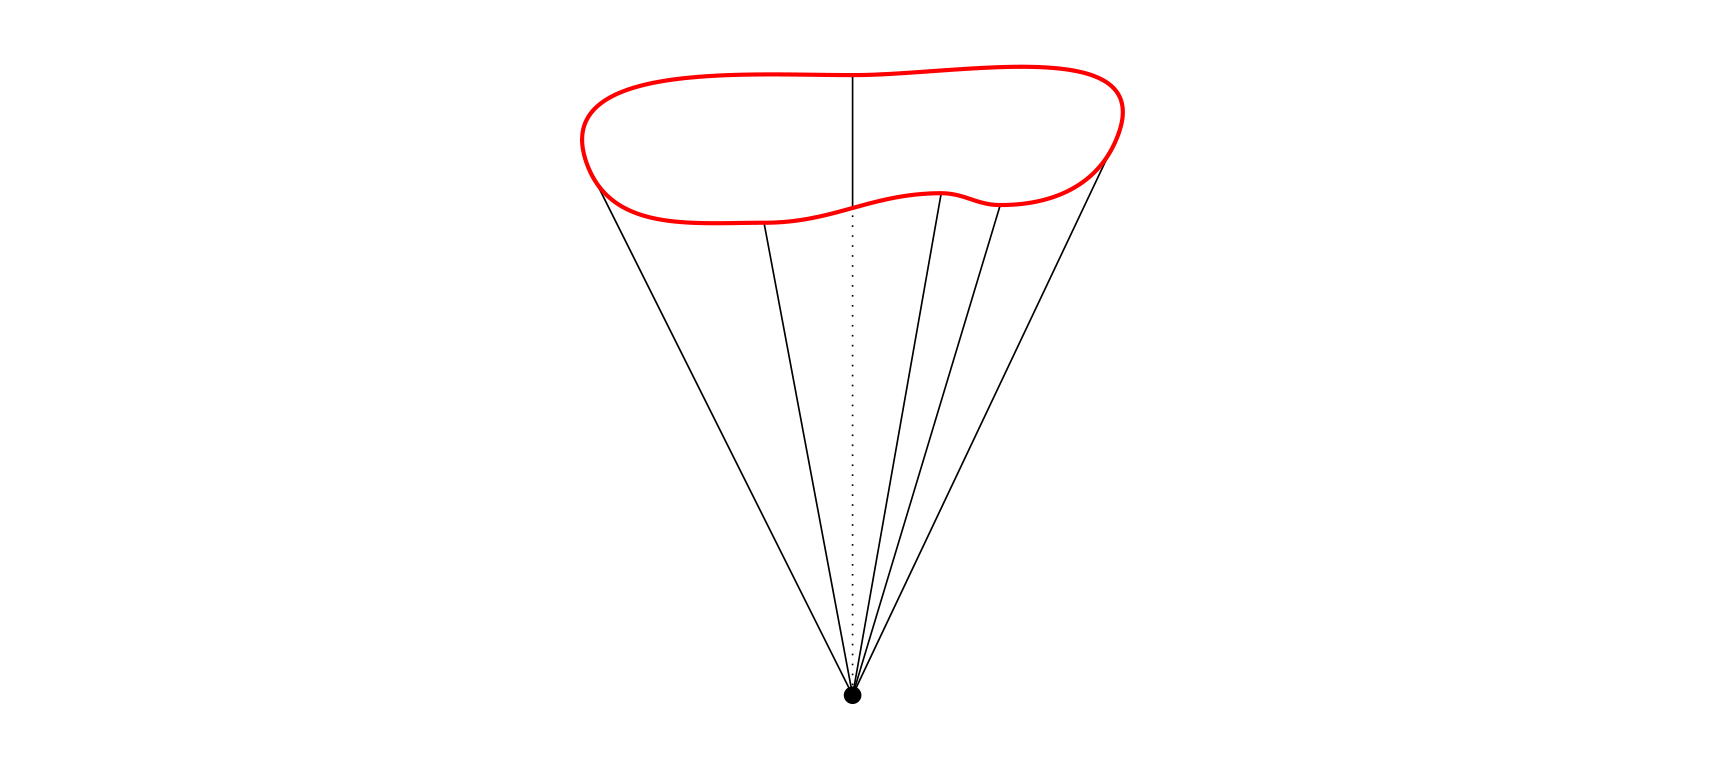
\includegraphics[width=0.42\textwidth]{figure10-7.png}
  \caption{流形 $M$ 的锥：先把 $M$ 与一个区间作乘积，然后把一端上整个 $M$ 的拷贝商掉。原来的流形用红色标出。（原文 p.~161，Figure 10.7）}
  \label{fig:10-7}
\end{figure}

给定流形 $M$，我们可以通过构造 $M$ 上的\term{锥}{cone}来造出奇点，其定义为：
\begin{equation}\tag{10.159}
C(M):=(M\times I)\big/(M\times\{0\}),
\end{equation}
如图~10.7。奇异点周围的链环是 $M$。我们想加入同样风味的奇点。例如，我们可能允许链环由某个流形给出的奇点，或者做某种分层版本，用这样的锥归纳地构造。

带奇点的配边假设粗略地说：从带可能的 $C(M)$-奇点的 $\Bord_n$ 到 $(\mathcal{C},\otimes)$ 的对称幺半函子，等价于：
\begin{enumerate}
\item $\mathcal{Z}\colon\Bord_n\to\mathcal{C}$（或等价地，一个对象 $C\in\mathcal{C}$），连同
\item $\mathcal{Z}(M)$ 的一个对象，即一个态射：
\begin{equation}\tag{10.160}
1\longrightarrow\mathcal{Z}(M).
\end{equation}
\end{enumerate}
想法是：$M$ 上的锥是一条从 $\varnothing$ 到 $M$ 的新配边，$\mathcal{Z}$ 把它送到映射 $1\to\mathcal{Z}(M)$，即 $\mathcal{Z}(M)$ 的一个元素。我们唯一需要的情形是 $M$ 为球面。当我们取以球面为模型的锥时，这其实并不是真正的奇点，但我们仍然可以想象：在构造以球面为模型的锥时指定了一个标记点。例如，如果我们看带标记点的 $\Bord_n$，那么带奇点的配边假设说这个标记点等价于指定一个对象 $\mathcal{O}\in\mathcal{Z}\big(S^{n-1}\big)$，而这是一个局部算子。所以这就是我们已经看到的东西。如果你愿意，这就是局部算子的态—场对应。

这告诉我们：如果我们看 $n$-流形连同嵌入的 $(k-1)$-流形，那么我们需要看奇点的链环（即嵌入子流形），它是一个球面 $S^{n-k}$。所以我们需要给出 $\mathcal{Z}\big(S^{n-k}\big)$ 的一个元素。这些被称为\term{缺陷算子}{defect operator}。例如，线缺陷/线算子是嵌入的 $1$-流形，它们对应于一个态的选择
\begin{equation}\tag{10.161}
L\in\mathcal{Z}\big(S^{n-2}\big).
\end{equation}
所以以前局部算子是向量空间 $\mathcal{Z}\big(S^{n-1}\big)$ 的元素，而现在赋值 $\mathcal{Z}\big(S^{n-2}\big)$ 是线算子的范畴。同样地，$\mathcal{Z}\big(S^{n-3}\big)$ 是曲面缺陷的 $2$-范畴。

要点是：给定 $n$ 维 TFT $\mathcal{Z}$，一旦我们指定了一个元素 $L\in\mathcal{Z}\big(S^{n-2}\big)$（满足适当的可对偶性条件），我们就可以把理论延拓到带任意嵌入 $1$-流形的流形上。也就是说，对任意纽结 $K\subset M$，我们得到新的值：
\begin{equation}\tag{10.162}
\mathcal{Z}_L(M\supset K).
\end{equation}

\begin{srcex}{63}
若 $n=3$，这就是说：我们需要指定一个元素 $L\in\mathcal{Z}\big(S^{n-2}\big)$ 来确定一个纽结不变量。
\end{srcex}

我们看到 $\mathcal{Z}\big(S^{n-1}\big)$ 构成交换环（$n\ge2$），然后取 $\Spec$：
\begin{equation}\tag{10.163}
\mathcal{M}_{\mathcal{Z}}^{0}=\Spec\mathcal{Z}\big(S^{n-1}\big),
\end{equation}
并在其上谱分解，即把态研究成局部算子上的模。

现在我们要对线算子玩同样的游戏。所以考虑线算子的范畴 $\mathcal{Z}\big(S^{n-2}\big)$。事实上，正如局部算子的向量空间构成代数那样，它也构成一个张量范畴。这个乘积仍然来自所谓的 OPE，但现在是线算子的 OPE 而不是局部算子的。乘积来自图~10.3 中的配边，只不过现在我们把它看成生活在四维空间中，即球面是 $n$ 维空间中绕两条嵌入线的链环 $S^{n-2}$（而不是 $n$ 维空间中绕两个点的链环 $S^{n-1}$）。

换句话说，得到这个结构所需的数据是（更大的）圆盘内部点（或圆盘）的构型。这与我们为局部算子画过的图是同一幅，只是我们现在忽略了更多的维数，所以范畴的层级跳了一级。也就是说，$\mathcal{Z}\big(S^{n-2}\big)$ 带有由“大圆盘内一对圆盘”的构型（局部常值地）标记的乘法。（这意味着它定义在小 $(n-1)$-圆盘算子之上，后者也称为 $E_{n-1}$-结构。）

\begin{srcex}{64}
例如，二维的线算子是余维 $1$ 的，于是我们有由区间内的区间标记的乘法。所以乘法是结合的但不交换。这是一个 $E_1$-结构。
\end{srcex}

\begin{srcex}{65}
在三维中我们有“马裤”：
\diageq{10.164}{0.13\textwidth}{p163_d1.png}
它是从 $S^1\sqcup S^1$ 到 $S^1$ 的配边，因此告诉我们 $\mathcal{Z}\big(S^1\big)$ 有一个运算 $*$，它局部常值地依赖于圆盘内两点的构型空间。更精确地说，我们是指：给定构型之间的一条路径，我们就得到相应乘法之间的一个同构。也就是说，我们得到从基本群胚出发的映射：
\begin{equation}\tag{10.165}
\pi_{\le1}\big(\mathrm{Conf}_2 D^2\big)\otimes\mathcal{Z}\big(S^1\big)^{\otimes2}\longrightarrow\mathcal{Z}\big(S^1\big).
\end{equation}
\end{srcex}
圆盘中两点对的这个空间是连通的，所以在局部算子层面这个乘法是交换的。现在这只说明我们有一个同构 $L_1*L_2\simeq L_2*L_1$，但当我们把它平方时，并不能保证得到恒等：
\begin{equation}\tag{10.166}
L_1*L_2\xrightarrow{\ \sim\ }L_2*L_1\xrightarrow{\ \sim\ }L_1*L_2
\qquad\big(\text{复合是否为 }\mathrm{id}?\big)
\end{equation}
于是我们发现：$\mathcal{Z}\big(S^1\big)$ 仍是幺半的，但现在它甚至是\term{辫状幺半}{braided monoidal}的，即这个乘法运算满足辫关系。我们可以想象圆盘中多个点的构型通过一个辫变成另一个构型：
\diageq{10.167}{0.16\textwidth}{p163_d3.png}
这给出一个同构：
\begin{equation}\tag{10.168}
L_1*L_2*L_3\longrightarrow L_3*L_2*L_1,
\end{equation}
而辫关系说这些同构满足辫群的关系。

所以在二维，线算子是 $E_1$，即一个幺半范畴。在三维，线算子是 $E_2$，即一个辫状幺半范畴。但在四维及以上，线算子是 $E_\infty$，即对称幺半的。于是基本群胚是：
\begin{equation}\tag{10.169}
\pi_{\le1}\big(\mathrm{Conf}_2 D^{\ge3}\big)=0,
\end{equation}
所以我们平方得到恒等：
\begin{equation}\tag{10.170}
L_1*L_2\xrightarrow{\ \sim\ }L_2*L_1\xrightarrow{\ \sim\ }L_1*L_2
\qquad\big(\text{复合 }=\mathrm{id}\big).
\end{equation}
也就是说，这些空间不只是连通的，事实上还是\emph{单连通}的。

% [Tutor Note: (10.163) 原文写的是 $\mathcal{M}^0_{\mathcal{Z}}=\Spec\mathcal{Z}(S^{m-1})$，上标 $m$ 与上下文（$n$ 维理论）不符，应为 $S^{n-1}$，这是原稿的笔误。(10.166) 与 (10.170) 的区别正是 $\pi_1$ 的作用：$D^2$ 中两点构型空间的基本群是 $\Z$（绕数），所以交换两次只给出辫关系而不保证恒等；而在 $\ge3$ 维，构型空间单连通，平方才是恒等，于是得到对称幺半 $E_\infty$。]

现在我们可以陈述结论了。在四维及以上，线算子：
\begin{equation}\tag{10.171}
\big(\mathcal{Z}\big(S^2\big),*\big)
\end{equation}
构成张量范畴，于是我们可以定义：
\begin{equation}\tag{10.172}
\mathcal{M}_{\mathcal{Z}}^{1}:=\Spec\Big(\mathcal{Z}\big(S^2\big),*\Big).
\end{equation}
这是 $\mathcal{M}_{\mathcal{Z}}^{0}$ 的一个加细。具体地说，它由仿射化给出：
\begin{equation}\tag{10.173}
\mathcal{M}_{\mathcal{Z}}^{1}\twoheadrightarrow\mathcal{M}_{\mathcal{Z}}^{0},
\qquad \mathcal{M}_{\mathcal{Z}}^{0}=\mathrm{Aff}\big(\mathcal{M}_{\mathcal{Z}}^{1}\big).
\end{equation}

% [Tutor Note: (10.171) 原文本应是一个范畴 $\big(\mathcal{Z}(S^2),*\big)$，而 (10.172) 才是对它的谱；这里把“取谱”的对象与谱本身分开写更清楚。$\mathcal{M}^1_{\mathcal{Z}}\to\mathcal{M}^0_{\mathcal{Z}}$ 是仿射化，一般不是同构：线算子比局部算子知道严格更多的信息（见 Remark 64）。]

\begin{flushright}\small（原稿批注：transition。）\end{flushright}

\begin{flushright}\small 第 24 讲；2021 年 4 月 22 日\end{flushright}

% ============================================================================
\subsection{局部算子与线算子}\label{sec:10-8-3}

\begin{sectionkey}
缺陷就是“流形上的标记子流形”，其余维为 $k$ 时由 $Z(S^{k-1})$ 标记。四维时线算子（余维 2）构成张量范畴，其谱 $\mathcal{M}^1_Z$ 是 $\mathcal{M}^0_Z$ 的仿射化；因此线算子严格比局部算子知道得更多。
\end{sectionkey}

回忆 TFT 中的缺陷算子是我们的 TFT 在各维球面上的值：
\begin{itemize}
\item $\mathcal{Z}\big(S^{n-1}\big)$ 由局部算子组成；
\item $\mathcal{Z}\big(S^{n-2}\big)$ 由线算子组成；
\item $\mathcal{Z}\big(S^{n-3}\big)$ 由曲面算子组成，等等。
\end{itemize}
当 $n$（理论的维数）足够大而缺陷的维数足够小时，缺陷构成交换代数。也就是说，一旦球面有足够的空间互相绕行，“碰撞”得到的乘积就变成交换的。例如我们看到，对 $n=1$ 局部算子只是结合的；但对 $n>1$ 它们是交换的。类似地，线算子在 $n=2$ 时结合，$n=3$ 时辫状，$n\ge4$ 时对称。

我们主要关心四维 TFT 中的线算子。它们构成对称幺半范畴 $\big(\mathcal{Z}\big(S^2\big),*\big)$，于是我们取谱：
\begin{equation}\tag{10.174}
\mathcal{M}_{\mathcal{Z}}^{1}:=\Spec\Big(\mathcal{Z}\big(S^2\big),*\Big).
\end{equation}
回忆局部算子 $\mathcal{Z}\big(S^{n-1=3}\big)$ 构成交换代数，所以我们也可以对它取谱，得到：
\begin{equation}\tag{10.175}
\mathcal{M}_{\mathcal{Z}}^{0}=\Spec\mathcal{Z}\big(S^{n-1}\big).
\end{equation}

\textbf{问题 7.} $\mathcal{M}_{\mathcal{Z}}^{1}$ 与 $\mathcal{M}_{\mathcal{Z}}^{0}$ 之间的关系是什么？也就是说，线算子与局部算子之间的关系是什么？

看这个关系的一种方式是用下面这幅漫画。考虑一个局部算子，即大片的“空无一物”中间的一个蓝色小点：
\diageq{10.176}{0.12\textwidth}{p164_d2.png}

我们可以把它解释为：它其实坐在一条透明的、画成红色的线上：
\diageq{10.177}{0.12\textwidth}{p165_d1.png}
也就是说，我们把局部算子看成坐在一条\emph{平凡}的 $1$ 维缺陷上。这个平凡缺陷是线算子上卷积结构的单位。也就是说，\textbf{局部算子等同于平凡线算子的自界面}。

\paragraph{悬垂}

结果表明，这幅图像可以用“对球面作悬垂”来重新表述。假设我们在研究 $S^{n-2}$，它作为一条线的链环出现。那么线算子 $\mathcal{Z}\big(S^{n-2}\big)$ 有一个 特殊的对象：
\begin{equation}\tag{10.178}
\mathcal{Z}\big(D^{n-1}\big)\in\mathcal{Z}\big(S^{n-2}\big),
\end{equation}
因为我们可以把圆盘看成一个配边：
\diageq{10.179}{0.21\textwidth}{p165_d2.png}
即从 $S^{n-2}\to\varnothing$ 的配边。

断言是：这个 特殊的对象就是单位。回忆我们的乘法来自“马裤”配边：
\diageq{10.180}{0.12\textwidth}{p165_d3.png}
于是用圆盘作乘法就是恒等，因为一旦把“马裤”与圆盘复合起来，我们就得到：
\begin{equation}\tag{10.181}
\text{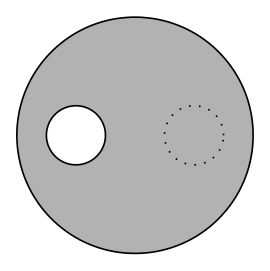
\includegraphics[width=0.10\textwidth]{p165_d4.png}}\;\simeq\;
\text{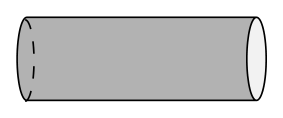
\includegraphics[width=0.10\textwidth]{p165_d5.png}}\;\simeq\;S^{n-2}\times I,
\end{equation}
而这是恒等配边。

我们也可以把圆盘与自身复合，形成一个球面：
\begin{equation}\tag{10.182}
\text{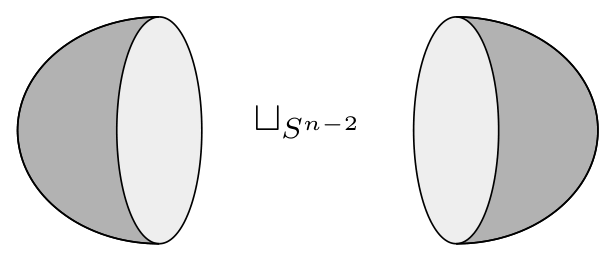
\includegraphics[width=0.15\textwidth]{p166_d1.png}}\;=\;
\text{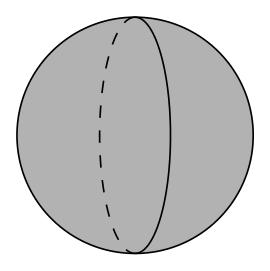
\includegraphics[width=0.09\textwidth]{p166_d2.png}}\;=\;S^{n-1}.
\end{equation}
这恰好就是把 $S^{n-2}$ 悬垂得到 $S^{n-1}$ 的过程。要点是：这幅图给出
\begin{equation}\tag{10.183}
\mathcal{Z}\big(S^{n-1}\big)=\Hom_{\mathcal{Z}(S^{n-2})}\Big(\mathcal{Z}\big(D^{n-1}\big),\mathcal{Z}\big(D^{n-1}\big)\Big)
=\End_{\mathcal{Z}(S^{n-2})}(1).
\end{equation}
也就是说，$\mathcal{Z}\big(S^{n-1}\big)$ 是 $\mathcal{Z}\big(S^{n-2}\big)$ 中单位的自同态。

\begin{srcrem}{62}
如果我们更小心地处理标架等等，圆盘的两份复合起来给出的是\emph{意大利饺}（ravioli）/UFO：
\begin{equation}\tag{10.184}
\text{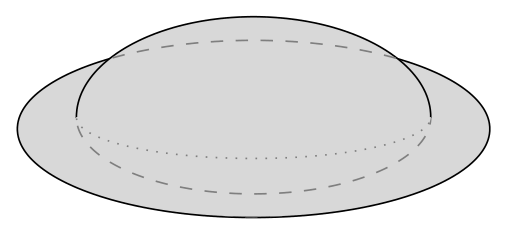
\includegraphics[width=0.15\textwidth]{p166_d3.png}}\;=\;
D^{n-1}\sqcup_{D^{n-1}\backslash\mathrm{pt}}D^{n-1}\;=\;
\text{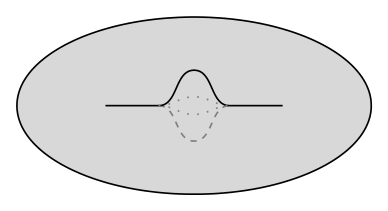
\includegraphics[width=0.12\textwidth]{p166_d4.png}}.
\end{equation}
\end{srcrem}

结论是：局部算子 $\mathcal{Z}\big(S^{n-1}\big)$ 被等同于：
\begin{equation}\tag{10.185}
\mathcal{Z}\big(S^{n-1}\big)=\End\big(1_{\mathcal{Z}(S^{n-2})}\big)=\End(\text{平凡线算子}).
\end{equation}

\begin{srcrem}{63}
这与 \S10.4.3、例~58、\S10.6.3、\S10.7（例~62）中的做法是同一招；在那里我们说：
\begin{equation}\tag{10.186}
\mathcal{Z}_G\big(S^1\big)=\C\left[\frac{G}{G}\right]=\End({}_G\C_G G),
\end{equation}
并把它中的 ${}_G\C_G G$ 解释为 $\mathcal{Z}_G$ 的平凡线缺陷。
\end{srcrem}

这对任意球面都是一般构造。例如，线算子由平凡曲面算子的自同态给出。

\paragraph{仿射化}

于是我们通过 TFT 看到了局部算子与线算子之间的关系，但现在我们想从谱的角度来看它。回忆我们有 $\mathcal{M}_{\mathcal{Z}}^{0}=\Spec\mathcal{Z}\big(S^{n-1}\big)$ 与 $\mathcal{M}_{\mathcal{Z}}^{1}=\Spec\mathcal{Z}\big(S^{n-2}\big)$。我们刚刚看到的是：$\mathcal{Z}\big(S^{n-1}\big)$ 由 $\mathcal{Z}\big(S^{n-2}\big)$ 中单位/平凡对象（即 $\big(\mathcal{M}_{\mathcal{Z}}^{1},\otimes\big)$）的自同态给出。我们知道 $\QC\big(\mathcal{M}_{\mathcal{Z}}^{1},\otimes\big)$ 中的单位是结构层：
\begin{equation}\tag{10.187}
\mathcal{O}_{\mathcal{M}_{\mathcal{Z}}^{1}}\in\QC\big(\mathcal{M}_{\mathcal{Z}}^{1},\otimes\big),
\end{equation}
所以这就是说：
\begin{align}
\mathcal{Z}\big(S^{n-1}\big)&=\mathcal{O}\big(\mathcal{M}_{\mathcal{Z}}^{0}\big)\tag{10.188}\\
&=\End_{\QC(\mathcal{M}_{\mathcal{Z}}^{1})}\big(\mathcal{O}_{\mathcal{M}_{\mathcal{Z}}^{1}}\big)\tag{10.189}\\
&=\Hom\big(\mathcal{O}_{\mathcal{M}_{\mathcal{Z}}^{1}},\mathcal{O}_{\mathcal{M}_{\mathcal{Z}}^{1}}\big)\tag{10.190}\\
&=\Gamma\big(\mathcal{O}_{\mathcal{M}_{\mathcal{Z}}^{1}}\big),\tag{10.191}
\end{align}
因为从 $\mathcal{O}$ 到任何东西的 $\Hom$ 就是那个东西的整体截面。也就是说
\begin{equation}\tag{10.192}
\mathcal{M}_{\mathcal{Z}}^{0}=\Spec\Gamma\big(\mathcal{O}_{\mathcal{M}_{\mathcal{Z}}^{1}}\big)=:\mathrm{Aff}\big(\mathcal{M}_{\mathcal{Z}}^{1}\big),
\end{equation}
因为这就是仿射化的定义。这是代数几何中的一般构造：
\begin{equation}\tag{10.193}
X\longrightarrow\mathrm{Aff}(X):=\Spec\big(\mathcal{O}(X)\big),
\end{equation}
它在如下意义下是泛的：从 $X$ 到仿射簇的任何映射都经过到 $\mathrm{Aff}(X)$ 的映射分解。也就是说，给定一个概形（或栈），我们可以考虑其上的函数；这并不能知道关于它的一切（即大多数对象不是仿射的），但我们仍可以对它取 $\Spec$ 得到仿射化：一个“逼近”原概形的仿射对象。

于是我们有
\begin{equation}\tag{10.194}
\mathcal{M}_{\mathcal{Z}}^{1}\twoheadrightarrow\mathcal{M}_{\mathcal{Z}}^{0}
\end{equation}
是仿射化，即 $\mathcal{M}_{\mathcal{Z}}^{1}$ 是 $\mathcal{M}_{\mathcal{Z}}^{0}$ 的一个新的、改进的版本；也就是说，一般地，线算子严格知道得比局部算子多。

\begin{srcrem}{64}
仿射化可能丢掉大量信息。例如，射影空间 $\PP^{n}$ 的仿射化是一个点，而像 $BG$ 这样的栈的仿射化也是一个点。要点是：代数栈的世界远不止函数环。
\end{srcrem}

于是我们看到：取单位自同态这一范畴论操作，对应于悬垂这一拓扑操作，又对应于相应模空间的仿射化这一代数几何操作。

\begin{srcrem}{65}
我们还可以进一步构造与曲面算子相联系的某个对象 $\mathcal{M}_{\mathcal{Z}}^{2}$：
\begin{equation}\tag{10.195}
\cdots\longrightarrow\mathcal{M}_{\mathcal{Z}}^{2}\longrightarrow\mathcal{M}_{\mathcal{Z}}^{1}\longrightarrow\mathcal{M}_{\mathcal{Z}}^{0}.
\end{equation}
我们不需要这些更高的版本，但 $\mathcal{M}_{\mathcal{Z}}^{1}$ 的构造对我们非常有用。
\end{srcrem}

% [Tutor Note: (10.183)--(10.186) 的核心等式链是 $\mathcal{Z}(S^{n-1})=\End_{\mathcal{Z}(S^{n-2})}(1)$：局部算子是线算子范畴中单位的自同态。这就解释了为什么“局部算子环 = 线算子范畴的中心”。取 $\Spec$ 之后，$1\mapsto\mathcal{O}$（结构层），$\End(\mathcal{O})=\Gamma(\mathcal{O})$ 是整体截面，于是 $\mathcal{M}^0_{\mathcal{Z}}=\Spec\Gamma(\mathcal{O}_{\mathcal{M}^1_{\mathcal{Z}}})$ 恰是仿射化。(10.186) 中 ${}_G\C_G G$ 是双模记号（群的左、右作用）。]

从一个四维 TFT 我们构造了栈 $\mathcal{M}_{\mathcal{Z}}^{1}$，即 TFT $\mathcal{Z}$ 的谱。这对于下面的事情很有用。想法是：这给出我们用所谓 B-模型（\S10.7 引入的简单拉格朗日 TFT）所作的逼近以及与它们的关系。也就是说，我们可以问：$\mathcal{Z}$ 与“映入其模空间/谱 $\mathcal{M}_{\mathcal{Z}}^{1}$ 的映射理论”有多接近？设 $X$ 是簇或栈。回忆对任意 $n$，我们可以构造 $n$ 维截断 TFT，称为 B-模型 $B_X^{n}$，它把 $(n-1)$-流形送到：
\begin{equation}\tag{10.196}
B_X^{n}\big(M^{n-1}\big)=\mathcal{O}\big(\mathrm{Map}_{\mathrm{lc}}(M,X)\big),
\end{equation}
其中映射（场）是局部常值的。对 $X$ 是栈的情形，我们可以做一些比简单构造
\begin{equation}\tag{10.197}
\mathrm{Map}_{\mathrm{lc}}(M,X)=\mathrm{Map}(\pi_0M,X)
\end{equation}
更有意思的事（这是 $X$ 只是簇时我们做的）。回忆栈是函子 $\mathrm{Ring}\to\mathrm{Grpd}$。对 $M$ 为流形，我们可以构造基本群胚
\begin{equation}\tag{10.198}
\pi_{\le1}M,
\end{equation}
其对象是点，态射是模同伦的路径。于是现在我们可以把局部常值映射解释为：
\begin{equation}\tag{10.199}
\mathrm{Map}_{\mathrm{lc}}(M,X)=\mathrm{Map}(\pi_{\le1}M,X).
\end{equation}
要点是：任何流形 $M$ 给出一个函子 $\mathrm{Ring}\to\mathrm{Grpd}$，它就是常函子
\begin{equation}\tag{10.200}
R\mapsto\pi_{\le1}(M).
\end{equation}
因此我们可以把流形与栈看成生活在
\begin{equation}\tag{10.201}
\mathrm{Functors}(\mathrm{Ring},\mathrm{Grpd})
\end{equation}
中。现在我们可以在函子的这个公共范畴中计算 $\mathrm{Map}_{\mathrm{lc}}(M,X)$。其结果是：这些映射记住了 $M$ 的基本群胚，而不仅仅是 $\pi_0$。

\begin{srcex}{66}
设 $X=\mathrm{pt}/G$，$G$ 有限。则
\begin{equation}\tag{10.202}
\mathrm{Map}_{\mathrm{slc}}(M,\mathrm{pt}/G)=\Loc_G M.
\end{equation}
于是 $X$ 的 B-模型由把这个空间 $\mathrm{Map}_{\mathrm{lc}}(M,X)$ 线性化给出：
\begin{align}
B_X^{n}\big(M^{n-1}\big)&=\mathcal{O}\big(\mathrm{Map}_{\mathrm{lc}}(M,X)\big)\tag{10.203}\\
B_X^{n}\big(N^{n-2}\big)&=\QC\big(\mathrm{Map}_{\mathrm{lc}}(N,X)\big)\tag{10.204}\\
B_X^{n}\big(P^{n-3}\big)&=\mathrm{ShvCat}\big(\mathrm{Map}_{\mathrm{lc}}(P,X)\big).\tag{10.205}
\end{align}
\end{srcex}

\paragraph{故事的寓意}

于是我们从 $n$ 维 TFT $\mathcal{Z}$ 出发，构造了谱 $\mathcal{M}_{\mathcal{Z}}^{1}$。由它可以构造两样东西：$B_{\mathcal{M}_{\mathcal{Z}}^{1}}^{n}$ 或 $B_{\mathcal{M}_{\mathcal{Z}}^{1}}^{n+1}$。于是 $\mathcal{Z}$ 在代数几何中最好的逼近是 $B_{\mathcal{M}_{\mathcal{Z}}^{1}}^{n}$。更好的认识是：$\mathcal{Z}$ 在 $\mathcal{M}_{\mathcal{Z}}^{1}$ 上线性，即 $\mathcal{Z}$ 是 $B_{\mathcal{M}_{\mathcal{Z}}^{1}}^{n+1}$ 的边界。

回忆 $\mathcal{Z}\big(N^{n-2}\big)$ 被 $\mathcal{Z}\big(S^{n-2}\big)$ 作用，于是我们发现：对 $N^{n-2}$ 的每一点，$\mathcal{Z}\big(N^{n-2}\big)$ 都有 $\mathcal{Z}\big(S^{n-2}\big)$ 上的模结构。也就是说，不做任何选择，我们就得到 $\mathcal{Z}\big(S^{n-2}\big)$ 的 $\pi_0(N)$ 多份拷贝的一个作用。但实际上我们可以把 $\pi_0$ 换成 $\pi_{\ge1}$。所以之前我们有的是：若两点之间存在通路，则相应的作用同构。现在我们有的是：对它们之间的每条路径都有一个作用之间的同构。也就是说，模结构关于 $x\in N$ 局部常值，于是我们实际上有“从 $N$ 到模空间的局部常值映射”的 $\QC$ 的作用：
\begin{equation}\tag{10.206}
\mathcal{Z}\big(N^{n-2}\big)\curvearrowright\QC\big(\mathrm{Map}_{\mathrm{lc}}(N,\mathcal{M}_{\mathcal{Z}}^{1})\big).
\end{equation}
也就是说，我们有一个范畴 $\mathcal{Z}\big(N^{n-2}\big)$，还有另一个范畴
\begin{equation}\tag{10.207}
B_{\mathcal{M}_{\mathcal{Z}}^{1}}^{n}(N)=\QC\big(\mathrm{Map}_{\mathrm{slc}}(N,\mathcal{M}_{\mathcal{Z}}^{1})\big),
\end{equation}
而前者是后者的模。即 $\mathcal{Z}\big(N^{n-2}\big)$ 是 $B_{\mathcal{M}_{\mathcal{Z}}^{1}}^{n}(N)$ 的一个对象，后者是 $\mathcal{M}_{\mathcal{Z}}^{1}$ 上的范畴层。

\begin{srcrem}{66}
这是把所有这些线算子装配成作用于 $\mathcal{Z}\big(N^{n-2}\big)$ 的对象的一般方式。这个过程称为\term{因子化同调}{factorization homology}。常用如下记号：
\begin{align}
\int_M R&=\mathcal{O}\big(\mathrm{Map}_{\mathrm{lc}}(M,\Spec(R))\big),\tag{10.208}\\
\int_M (\mathcal{C},\otimes)&=\QC\big(\mathrm{Map}_{\mathrm{slc}}(M,\Spec(\mathcal{C}))\big),\tag{10.209}
\end{align}
后者是范畴的情形。
\end{srcrem}

现在我们将看到 $\mathrm{Map}_{\mathrm{slc}}(N,\mathcal{M}_{\mathcal{Z}}^{1})$ 具有恰当类型的结构。对一点 $x\in N$ 我们得到求值映射：
\begin{equation}\tag{10.210}
\begin{array}{c}
\mathrm{Map}_{\mathrm{lc}}(N,\mathcal{M}_{\mathcal{Z}}^{1})\\[2pt]
\downarrow{\scriptstyle \mathrm{ev}_x}\\[2pt]
\mathcal{M}_{\mathcal{Z}}^{1}
\end{array}
\end{equation}
于是我们得到拉回映射：
\begin{equation}\tag{10.211}
\mathrm{ev}_x^{*}\colon \QC\big(\mathcal{M}_{\mathcal{Z}}^{1}\big)\longrightarrow\QC\big(\mathrm{Map}_{\mathrm{lc}}(N,\mathcal{M}_{\mathcal{Z}}^{1})\big).
\end{equation}
所以如果我们有 $\QC\big(\mathrm{Map}_{\mathrm{lc}}(N,\mathcal{M}_{\mathcal{Z}}^{1})\big)$ 在 $\mathcal{Z}\big(N^{n-2}\big)$ 上的作用，我们也得到 $\QC\big(\mathcal{M}_{\mathcal{Z}}^{1}\big)$ 的作用：
\begin{equation}\tag{10.212}
\mathrm{ev}_x^{*}\colon \QC\big(\mathcal{M}_{\mathcal{Z}}^{2}\big)=\mathcal{Z}\big(S^{n-2}\big)\longrightarrow
\QC\big(\mathrm{Map}_{\mathrm{lc}}(N,\mathcal{M}_{\mathcal{Z}}^{2})\big)\curvearrowright\mathcal{Z}\big(N^{n-2}\big).
\end{equation}

\begin{srcrem}{67}
这个图表告诉我们这个操作的局部—整体相容性。也就是说：我们从与点 $x\in N$ 相联系的这些作用出发，它们装配在一起给出更大空间 $\QC\big(\mathrm{Map}_{\mathrm{lc}}(N,\mathcal{M}_{\mathcal{Z}}^{1})\big)$ 的一个作用，然后这些求值映射再把局部的作用取回来。
\end{srcrem}

局部—整体部分要证明的一般定理是：带有对每个 $x\in N$（局部常值地依赖于 $x$）的 $(\mathcal{C},\otimes)$ 的作用的范畴，等价于带有如下作用的范畴：
\begin{equation}\tag{10.213}
\mathcal{C}^{\otimes N}:=\int_N\mathcal{C}:=\QC\big(\mathrm{Map}_{\mathrm{slc}}(N,\Spec\mathcal{C})\big),
\end{equation}
其中 $\mathcal{C}$ 是 Tannakian 的（$\mathcal{C}=\QC(\Spec\mathcal{C})$）。

所以结论是：任意 $n$ 维 TFT $\mathcal{Z}$ 都是 $B_{\mathcal{M}_{\mathcal{Z}}^{1}}^{n+1}$ 的边界条件，即 $\mathcal{Z}(N)$ 在 $\mathrm{Map}_{\mathrm{lc}}(N,\mathcal{M}_{\mathcal{Z}}^{1})$ 上成层。

% [Tutor Note: (10.212) 中的 $\mathcal{M}^2_{\mathcal{Z}}$ 疑为 $\mathcal{M}^1_{\mathcal{Z}}$ 的笔误：这一段的语境全是线算子的谱 $\mathcal{M}^1_{\mathcal{Z}}$ 与 $\mathcal{Z}(S^{n-2})$，而 $\mathcal{M}^2_{\mathcal{Z}}$ 直到 Remark 65 才作为曲面算子的对象正式定义、且并未再使用。照译并指出。另注意 $\mathrm{Map}_{\mathrm{lc}}$ 与 $\mathrm{Map}_{\mathrm{slc}}$（带基本群胚的局部常值映射）的区别正是 (10.199) 与 (10.202) 的差别。]

% ============================================================================
\subsection{回到拓扑 Maxwell 理论}\label{sec:10-8-4}

\begin{sectionkey}
用上一节的抽象机器处理 4 维拓扑 Maxwell 理论 $\mathcal{A}_{\mathrm{GL}_1}$：其线算子是 $\Z$-分次向量空间，谱是 $\mathrm{pt}/\mathbb{G}_m$，于是电侧 $\QC(\Loc_1\Sigma)$ 作用在磁侧 $\mathcal{A}(\Sigma)$ 上。Fourier 变换把这个作用说成“$\mathcal{A}(\Sigma)$ 是 $\mathcal{B}(\Sigma)$ 上的秩 $1$ 自由模”。
\end{sectionkey}

回忆（来自 \S4.5、\S4.8.1、\S6.1.1 与 \S6.4）我们有一个 TFT $\mathcal{A}_{\mathrm{GL}_1}$，它把三维流形送到 $\mathrm{Pic}(M)$ 上的局部常值函数空间。对 Riemann 曲面我们有几个不同的版本。Betti 版本是：
\begin{equation}\tag{10.214}
\mathcal{A}_{\mathrm{GL}_1}\big(\Sigma^2\big)=\Loc\big(\mathrm{Pic}\,\Sigma\big),
\end{equation}
而在 de Rham 版本中我们有：
\begin{equation}\tag{10.215}
\mathcal{A}_{\mathrm{GL}_1}\big(\Sigma^2\big)=\mathbf{D}\text{-}\mathbf{Mod}\big(\mathrm{Pic}\,\Sigma\big).
\end{equation}
回忆这两个范畴并不相同，但非常相似。对于我们眼下要做的事，选哪一个都无所谓。

于是，靠上述抽象废话，对每一点 $x\in\Sigma^2$ 我们都得到 $\mathcal{A}(S^2)$（线算子）在 $\mathcal{A}(\Sigma^2)$ 上的作用。对 $S^2=\Sigma$ 我们选取一个复结构，于是可以把它想成 $\PP^1$，并且有
\begin{equation}\tag{10.216}
\mathcal{A}\big(S^1\big)=\Loc\big(\mathrm{Pic}(\PP^1)\big)=\Loc(\Z)=\Vect^{\Z\text{-gr}},
\end{equation}
其中复合积就是分次向量空间的张量积，即由 $\Z$ 上的群结构诱导的乘积。我们可以把这理解为：当我们有时……

\begin{srcrem}{68}
复合积由整数加法诱导，这一事实是 Gauss 定律的一个版本。这个复合积由配边 $\PP^1\sqcup\PP^1\to\PP^1$ 诱导（即从一个 $3$-球内部挖去两点）。我们可以想象在这两点处各有一个磁单极子，整数值被解释为它们的磁通量；然后当我们看得更远——即进入大的/目标 $\PP^1$ 内部——时，磁通量相加。
\end{srcrem}

也就是说，我们的线算子（'t Hooft/Dirac 线算子）对应于 $\Z$-分次向量空间。这告诉我们：我们的模空间由对 $\Vect^{\Z\text{-gr}}$ 作 Tannakian 重构给出。回忆例~37 中我们有：
\begin{equation}\tag{10.217}
\mathcal{M}_{\mathcal{A}_{\mathrm{GL}_1}}=\Spec\big(\Vect^{\Z\text{-gr}}\big)=\mathrm{pt}/\mathbb{G}_m.
\end{equation}
因此：
\begin{align}
\mathrm{Map}_{\mathrm{lc}}\big(\Sigma,\mathcal{M}_{\mathcal{A}}^{1}\big)&=\mathrm{Map}_{\mathrm{lc}}\big(\Sigma,\mathrm{pt}/\mathbb{G}_m\big)\tag{10.218}\\
&=\Loc_1(\Sigma).\tag{10.219}
\end{align}
所以我们发现 $\mathcal{A}(\Sigma^2)$ 被 $\QC(\Loc_1\Sigma)$ 作用，而回忆（来自 \S6.4.2）这正是 B-侧赋予曲面 $\Sigma$ 的东西：
\begin{equation}\tag{10.220}
\QC\big(\Loc_1\Sigma\big)=\mathcal{B}(\Sigma).
\end{equation}
于是我们发现：磁理论 $\mathcal{A}(\Sigma)$ 被电理论 $\mathcal{B}(\Sigma)$ 作用。但这并不是我们所说的。我们说过它们等价。于是我们接下来要说明的是：$\mathcal{A}(\Sigma)$ 是一个秩 $1$ 自由模，因此一旦选定一个生成元，它就同构于 $\mathcal{B}(\Sigma)$；也就是说，我们只需跟踪单位。

\begin{srcrem}{69}
我们讲了一阵子电磁对偶，把它说成涉及交换群论的 Fourier 变换。我们在这里发现的是：你并不真的需要那套交换群论。只从场论 $\mathcal{A}$ 出发，谱/电侧就是我们能内在地从 $\mathcal{A}$ 构造出来的东西。
\end{srcrem}

所以结论是：自守侧是
\begin{equation}\tag{10.221}
\mathcal{A}_G\big(\Sigma^2\big)=\Shv\big(\Bun_G(\Sigma)\big),
\end{equation}
（其中 $\mathcal{A}_G$ 是参数 $\Psi=0$ 的 GL-扭转 $\mathcal{N}=4$ 超 Yang--Mills 理论），然后由它我们构造某种谱侧 $\QC(-)$，后者作用在 $\mathcal{A}_G(\Sigma)$ 上。几何 Langlands 猜想说这两者是相同/密切相关的。

% [Tutor Note: (10.216) 左边原文印作 $\mathcal{A}(S^1)$，但线算子的链环在四维中是 $S^2$，且本段讨论的是 $S^2=\Sigma\cong\PP^1$ 上的线算子，故这里应为 $\mathcal{A}(S^2)$，是原稿的指标笔误。链路上：$\mathrm{Pic}(\PP^1)=\Z$ 是离散空间，其上的局部系统 (= $\Loc(\Z)$) 就是 $\Z$-分次向量空间，这正是 (10.216) 右边写成 $\Vect^{\Z\text{-gr}}$ 的原因；而 $\QC(\Loc_1\Sigma)$ 与 $\Loc(\mathrm{Pic}\,\Sigma)$ 是同一个范畴的两种描述（Tannakian / Fourier 对偶），这是几何 Langlands 中“电—磁”两侧的关键识别。]

\begin{flushright}\small 第 25 讲；2021 年 4 月 22 日\end{flushright}

% ============================================================================
\subsection{拓扑 Maxwell 理论}\label{sec:10-8-5}

\begin{sectionkey}
把对每一点的局部作用装配起来就是因子化同调 $\int_\Sigma R$；对 $\mathcal{A}_{\mathrm{GL}_1}$，这给出 $\QC(\Loc_{\mathbb{G}_m}\Sigma)$ 作用于磁侧。Fourier 变换的现代表述是“自守侧是谱侧的秩 $1$ 自由模”，由此进入几何 Langlands 的 Hecke 对应。
\end{sectionkey}

（原稿批注：transition。）回忆我们有一个四维 TFT $\mathcal{Z}$，对一个拓扑曲面 $\Sigma$，我们看 $\mathcal{Z}(\Sigma)$。它有一个对称代数，即局部算子代数 $\mathcal{Z}\big(S^2\big)$，它作用在 $\mathcal{A}(\Sigma)$ 上。特别地，对每一点 $x\in\Sigma$ 我们都可以挖去一个球：
\begin{equation}\tag{10.222}
x\in\Sigma\times\{i\}\subset\Sigma\times I
\end{equation}
得到一个配边 $\Sigma\sqcup S^2\to\Sigma$，$\mathcal{Z}$ 把它送到作用 $\mathcal{Z}\big(S^2\big)\otimes\mathcal{Z}(\Sigma)\to\mathcal{Z}(\Sigma)$。也就是说，对每一点 $x\in\Sigma$ 我们都得到一个作用。然后给定从 $x$ 到 $y$ 的一条路径，我们得到相应作用的等同；类似地，给定路径之间的路径（以此类推），我们得到等同之间的等同（以此类推）。于是从 TFT 我们得到一个交换代数（在范畴中）的作用，由 $x\in\Sigma$ 标记，关系由路径给出，关系之间的关系由路径之间的路径给出，以此类推。

这就是如下一般构造。给定交换代数 $R$（在任意带某些余极限的对称幺半（高阶）范畴 $(\mathcal{C},\otimes)$ 中）以及拓扑空间 $\Sigma$。那么，把 $\Sigma$ 只看成单纯集，我们可以构造 $R\otimes\Sigma$，它仍是 $\mathcal{C}$ 中的交换代数。简言之，它就是 $R^{\otimes\#\mathrm{vertices}(\Sigma)}$，关系由 $1$-单形给出，以此类推。这称为 $R$ 在 $\Sigma$ 上的\term{因子化同调}{factorization homology}，记作
\begin{equation}\tag{10.223}
\int_\Sigma R=R\otimes\Sigma.
\end{equation}
当交换环 $R$ 足够好（Tannakian）时，它有具体的几何描述：
\begin{equation}\tag{10.224}
R\otimes\Sigma=\mathcal{O}\big(\mathrm{Map}_{\mathrm{lc}}(\Sigma,\Spec(R))\big).
\end{equation}
对好的张量范畴 $R$（而不是交换环），我们有：
\begin{equation}\tag{10.225}
R\otimes\Sigma=\QC\big(\mathrm{Map}_{\mathrm{lc}}(\Sigma,\Spec(R))\big).
\end{equation}
现在我们将用它来研究规范理论。回忆我们处于拓扑 Maxwell 理论 $\mathcal{A}_{\mathrm{GL}_1}$ 的设定中。它没有局部算子，但有有意思的线算子，即余维 $3$ 缺陷。我们在 \S4.5.1 见过这些缺陷。给定三维流形 $M^3$，我们可以在一点处造一个 Dirac 磁单极子，并通过在这个点周围的 $2$-球面上给定某个磁通量，得到向量空间 $\mathcal{A}(M)$ 的一个新版本。同一想法的另一种变体如下。考虑 $M^3$ 并让时间流逝，即考虑 $M^3\times I$；余维 $3$ 的奇点将是 $M^3\times I$ 中的一个圈/纽结。这个奇点的链环将是 $S^2$，而现在我们可以研究这个柱面 $M^3\times I$ 上的丛，它们在 $2$-球面上有某个整的 Chern 类/通量。前一种线算子的表现修改了赋予 $M^3$ 的向量空间，后一种图像则给出 $\mathcal{Z}(M)$ 与自身之间的算子。

我们知道线算子组成 $\mathcal{Z}\big(S^2\big)$，在这个情形中它由下式给出：
\begin{equation}\tag{10.226}
\mathcal{A}_{\mathrm{GL}_1}\big(S^2\big)=\text{$\mathrm{Pic}(S^2)$ 上的层}=\Vect^{\Z\text{-gr}}.
\end{equation}
也就是说，给定三维流形 $M$、一点 $p\in M$ 以及一个 $\Z$-分次向量空间，我们得到赋予 $M$ 的 Hilbert 空间的一个新版本，它是按不同电荷/单极数加权的和。我们还有分次维数：
\begin{equation}\tag{10.227}
\dim_{\mathrm{gr}}\colon \Vect^{\Z\text{-gr}}\longrightarrow\C^{\Z},
\end{equation}
即给定 $\Z$-分次向量空间，我们得到整数的一个复线性组合。回忆我们在 $M\times I$ 中用单极数的复线性组合来标记纽结。所以这些分次向量空间给我们这些线算子，我们可以把它们绕在四维流形中真正的纽结/圈上。
% [Tutor Note: 这里的字典是：$\mathrm{Pic}(S^2)=\Z$ 是离散空间，其上的局部系统就是 $\Z$-分次向量空间，第 $k$ 个分量对应单极数 $k$ 的态；于是线算子范畴 $\mathcal{A}_{\mathrm{GL}_1}(S^2)=\Vect^{\Z\text{-gr}}$。(10.227) 的 $\dim_{\mathrm{gr}}$ 把每个分次维数读成一个整数，这正是把线算子绕在纽结上时按单极数加权的“迹”。[译者按（无外部依据）：由本章 (10.214)、(10.226)--(10.227) 及 Remark 68 的 Gauss 定律讨论推得]]

要点是：在规范理论中，余维 $3$ 缺陷有很大的活动空间。更详细地说：在 $3$ 维及以上我们可以看余维 $3$ 缺陷，其链环是 $2$-球面，而 $S^2$ 上 Yang--Mills 方程的解很有意思。这里我们谈的是交换情形，它只由单极数给出；现在我们将考虑非交换情形。这种一般类型的算子称为 \term{'t Hooft 算子}{'t Hooft operator}。

于是我们有：$\mathcal{A}_{\mathrm{GL}_1}(\Sigma)$ 被 $\Vect^{\Z\text{-gr}}$ 在每一点 $x\in\Sigma$ 处作用。我们可以把这些作用装配成 $\Sigma\otimes\Vect^{\Z\text{-gr}}$ 的作用，它可以写成：
\begin{align}
\Sigma\otimes\Vect^{\Z\text{-gr}}&=\Sigma\otimes\Rep(\mathbb{G}_m)\tag{10.228}\\
&=\Sigma\otimes\QC\big(\mathrm{pt}/\mathbb{G}_m\big)\tag{10.229}\\
&=\QC\big(\mathrm{Map}_{\mathrm{slc}}(\Sigma,\mathrm{pt}/\mathbb{G}_m)\big)\tag{10.230}\\
&=\QC\big(\Loc_{\mathbb{G}_m}(\Sigma)\big).\tag{10.231}
\end{align}
这个范畴正是 B-侧/电侧/谱侧赋予 $\Sigma$ 的东西：
\begin{equation}\tag{10.232}
\mathcal{B}_{\mathrm{GL}_1}(\Sigma):=\Sigma\otimes\mathcal{A}_{\mathrm{GL}_1}\big(S^2\big)=\QC\big(\Loc_{\mathbb{G}_m}(\Sigma)\big).
\end{equation}
所以 B/电/谱侧作用在 A/磁/自守侧上。一旦我们认识到 $\mathcal{A}$ 是 $\mathcal{B}$ 上的秩 $1$ 自由模，这就归结为“这些理论（在 Fourier 变换下）等价”的陈述。

我们可以在 Fourier 变换的层面看到这是如何运作的。我们习惯于 Fourier 变换给出同构：
\begin{equation}\tag{10.233}
\big(\mathrm{Fun}(G),*\big)\simeq\big(\mathrm{Fun}(G^{\vee}),\cdot\big),
\end{equation}
但我们可以把它重新表述为：$\mathrm{Fun}(G)$ 是 $\mathrm{Fun}(G^{\vee},\cdot)$ 上的秩 $1$ 模，带一个 特殊的单位。也就是说，我们有一个作用：
\begin{equation}\tag{10.234}
\big(\mathrm{Fun}(G^{\vee},\cdot)\big)\curvearrowright\mathrm{Fun}(G),
\end{equation}
由与特征作卷积给出。然后我们断言 $\mathrm{Fun}(G^{\vee})$ 事实上是秩 $1$ 自由模。对 $G$ 是群，$\delta_e\in\mathrm{Fun}(G)$ 是单位，所以我们可以作用在 $\delta_e$ 上得到：
\begin{equation}\tag{10.235}
\mathrm{Fun}(G^{\vee})\xrightarrow{\ \sim\ }\mathrm{Fun}(G).
\end{equation}
然后 Fourier 变换说这是同构。所以我们想把观点转变为以这种方式看待 Fourier 变换。

在 Betti 版本中，对 $\Sigma$ 为 Riemann 曲面，我们附上一个范畴：
\begin{equation}\tag{10.236}
\mathcal{A}_{\mathrm{GL}_1}(\Sigma)=\Loc\big(\mathrm{Pic}(\Sigma)\big).
\end{equation}
现在我们需要选一个单位，以便得到与“它作为模所依托的东西”的等同。我们想说的是 $\mathrm{Pic}$ 的单位处的摩天楼层层：$\mathcal{O}\in\mathrm{Pic}$。在 de Rham 版本中我们有 $\mathcal{A}_{\mathrm{GL}_1}(\Sigma)=\mathbf{D}\text{-}\mathbf{Mod}(\mathrm{Pic})$，所以我们可以直接取它。但在 Betti 版本中，这个摩天楼层层实际上并不在 $\Loc(\mathrm{Pic}(\Sigma))$ 中，所以我们需要找一个替代物如下。我们有包含：
\begin{equation}\tag{10.237}
i\colon\{\mathcal{O}\}\hookrightarrow\mathrm{Pic},
\end{equation}
然后我们可以取 $\mathrm{Pic}$ 的万有覆盖（关于基点 $\mathcal{O}$），它给出一个可缩空间 $\widetilde{\mathrm{Pic}}$ 映射到 $\mathrm{Pic}$：
\begin{equation}\tag{10.238}
\begin{array}{ccc}
\{\mathcal{O}\} & \xrightarrow{\ i\ } & \mathrm{Pic}\\[4pt]
& \searrow{\scriptstyle \widetilde{\pi}} & \uparrow{\scriptstyle \widetilde{\pi}}\\[4pt]
& & \widetilde{\mathrm{Pic}}
\end{array}
\end{equation}
% [Tutor Note: 图中 $\{\mathcal{O}\}\to\mathrm{Pic}$ 是包含 $i$；两条标作 $\widetilde{\pi}$ 的箭头分别是基点的提升 $\{\mathcal{O}\}\to\widetilde{\mathrm{Pic}}$ 与覆盖投影 $\widetilde{\mathrm{Pic}}\to\mathrm{Pic}$，二者复合即 $i$。正因为 $\widetilde{\mathrm{Pic}}$ 可缩，常层 $k$ 在它上面就是“平凡数据”，沿 $\widetilde{\pi}$ 前推（(10.239) 的 $\widetilde{\pi}_*(k)$）便得到 $\Loc(\mathrm{Pic})$ 中一个并非有限秩的局部系统——它是 de Rham 版本中单位处摩天楼层层的替身。[译者按（无外部依据）：由本章 (10.237)--(10.241) 与 Example 67 的 $p_*k$ 构造推得]]
然后我们把常层前推，得到单位：
\begin{equation}\tag{10.239}
\widetilde{\pi}_*(k)\in\Loc\big(\mathrm{Pic}(\Sigma)\big).
\end{equation}

\begin{srcex}{67}
回忆 $\Loc(S^1)\simeq\QC(\mathbb{G}_m)$。单位 $\mathcal{O}_1\in\QC(\mathbb{G}_m)$ 对应于圆周上如下局部系统。考虑万有覆盖：
\begin{equation}\tag{10.240}
p\colon\R\longrightarrow S^1.
\end{equation}
然后我们可以把常层前推，得到对应于单位的局部系统：
\begin{equation}\tag{10.241}
p_*k.
\end{equation}
这是一个有点奇怪的对象，例如它不是有限秩的（任意点上的纤维是 $\Z$），但断言是：作用在这个单位对象上给出 Fourier 变换。
\end{srcex}

理论 $\mathcal{A}_G$ 将线性化 $\Bun_G$，其中 $G$ 是 $\C$ 上的约化群（例如 $\mathrm{GL}_n(\C)$、$\mathrm{SO}_n(\C)$、$\mathrm{Sp}_n(\C)$、$E_8$ 等等）。口号是：理论 $\mathcal{A}_G$ 研究 $\Bun_G$ 的\emph{拓扑}。

\begin{srcex}{68}
对 $F$ 为数域，回忆 \S5.2.2：
\begin{equation}\tag{10.242}
\mathcal{A}_G\big(\Spec\mathcal{O}_F\big)=H^{*}\big(\Bun_G(\Spec\mathcal{O}_F)\big),
\end{equation}
其中我们写：
\begin{equation}\tag{10.243}
\Bun_G(\Spec\mathcal{O}_F)=G(F)\backslash G(\mathbb{A})/G(\mathcal{O}_{\mathbb{A}}).
\end{equation}
\end{srcex}

\begin{srcex}{69}
对函数域 $C/\F_q$，我们可以研究 $\Bun_G$ 上紧支撑的复值函数：
\begin{equation}\tag{10.244}
C_c\big[\Bun_G(C)(\F_q)\big].
\end{equation}
\end{srcex}

于是我们把 $\mathcal{A}_G$ 想成一个线性化 $G$-丛空间的理论。存在一个良定义的四维 TFT $\mathcal{A}_G$（物理意义下），称为规范群为 $G_c$（$G$ 的紧形式）的“A-扭转”四维 $\mathcal{N}=4$ 超 Yang--Mills 理论。这在开创性论文 [KW07] 中研究过。$\mathcal{A}_G$ 没有完全成熟的数学定义，但我们确实知道如何在曲面上赋值。若 $C$ 是 Riemann 曲面，我们研究模栈 $\Bun_G(C)$，并附上一个层范畴：
\begin{equation}\tag{10.245}
\Shv\big(\Bun_G(C)\big),
\end{equation}
它将有各种风味（Betti（可构造层）、de Rham（D-模）、restricted 等等），但它们总是拓扑层。所以我们研究的是 $\Bun_G(C)$ 的拓扑，而不是它的代数几何。

现在关键点是：我们可以研究 $\mathcal{A}_G$ 中的线算子。

\begin{srcrem}{70}
“没有”局部算子（除非在某种导出意义下，而且即使如此也不太有意思），所以线算子才是一切有趣事情发生的地方。
\end{srcrem}

主要原则是研究 't Hooft 单极。即：Yang--Mills 理论中有有意思的余维 $3$ 奇点，它们对应于研究四维空间中一条线的链环，即 $2$-球面。线算子由这个球面上的 $G$-丛标记，选定复结构后我们可以把它看成 $\PP^1$。Grothendieck--Birkhoff 分解告诉我们 $\PP^1$ 上丛的如下事实。为简单起见取 $G=\mathrm{GL}_n$。分解说：若 $V$ 是 $\PP^1$ 上的 $\mathrm{GL}_n$-丛（秩 $n$ 向量丛），则 $V$ 是线丛的直和：
\begin{equation}\tag{10.246}
V\simeq L_1\oplus L_2\oplus\cdots\oplus L_n,
\end{equation}
唯一到置换。换言之，它的点与 $\mathrm{GL}_n$ 相伴的余权格双射：
\begin{equation}\tag{10.247}
\Bun_n\PP^1\simeq\Z^n/S_n,
\end{equation}
其中 $S_n$ 是对称群。于是 $\PP^1$ 上这些向量丛都给我有意思的线算子，并由某种组合对象标记。

我们想用代数几何来写这个，但问题在于我们把曲面 $C$ 与时间区间 $I$ 作乘积，而从代数几何的角度这并不真的说得通。所以我们将通过坍缩时间维来重新解释这幅图：
\begin{equation}\tag{10.248}
\text{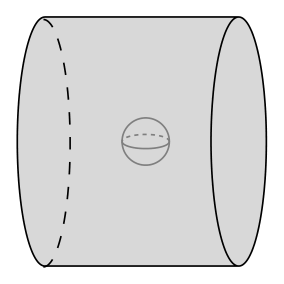
\includegraphics[width=0.10\textwidth]{p174_d1.png}}\quad;\quad
\text{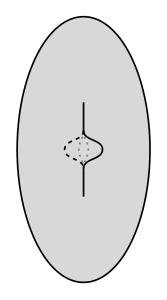
\includegraphics[width=0.055\textwidth]{p174_d2.png}}.
\end{equation}
形式上，当我们坍缩时间时，我们从
\begin{equation}\tag{10.249}
(C\times I)\setminus x\ \rightsquigarrow\ C\sqcup_{C\setminus x}C
\end{equation}
过渡。

回忆我们可以把局部算子看成平凡线缺陷的自同态。坍缩时间之后，这幅图告诉我们同一陈述的高维版本：\textbf{线算子是平凡曲面缺陷的自同态}。即考虑平凡曲面缺陷：
\begin{equation}\tag{10.250}
\{x\}\times I\times\R\subset C\times I\times\R.
\end{equation}
那么线缺陷 $\{x\}\times\{i\}$ 可以看成平凡曲面缺陷的一个自同态。要点是：当我们改为把线算子看成来自 $C\sqcup_{C\setminus x}C$ 时，它仍然是平凡曲面缺陷的自同态。

我们可以描述 $C\sqcup_{C\setminus x}C$ 上的 $G$-丛：
\begin{align}
\Bun_G\big(C\sqcup_{C\setminus x}C\big)&=\Bun_G(C)\times_{\Bun_G(C\setminus x)}\Bun_G(C)\tag{10.251}\\
&=\Big\{P_1,P_2\in\Bun_G(C),\ P_1|_{C\setminus x}\xrightarrow{\ \sim\ }P_2|_{C\setminus x}\Big\},\tag{10.252}
\end{align}
即这样的丛由 $C$ 上的一对丛以及在 $x$ 之外的同构组成。有一个 $G$-丛空间（即我们理论的场）的对应：
\begin{equation}\tag{10.253}
\begin{array}{ccc}
& \mathrm{Hecke}_x=\Bun_G\big(C\sqcup_{C\setminus x}C\big) &\\[4pt]
\swarrow & & \searrow\\[4pt]
\Bun_G(C) & & \Bun_G(C).
\end{array}
\end{equation}
于是我们可以把这个对应看成通过对 $\Bun_G$ 的任何线性化作推—拉来定义其上的算子。这就是我们解释线算子作用的方式。显式地
\begin{equation}\tag{10.254}
\mathcal{A}_G(C)=\Shv\big(\Bun_G(C)\big)
\end{equation}
（对某种拓扑的层概念），然后我们将用这个 Hecke 对应的推—拉在其上构造算子。

我们可以把从 $C$ 到 $C\sqcup_{C\setminus x}C$ 的过渡看成粘一个气泡：
\begin{equation}\tag{10.255}
D\sqcup_{D\setminus x}D\;=\;\text{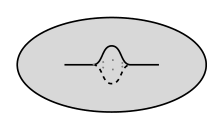
\includegraphics[width=0.075\textwidth]{p175_d3.png}}
\end{equation}
粘到 $C$ 上、沿 $x\in C$ 周围的某个圆盘 $D$：
\begin{equation}\tag{10.256}
C\sqcup_{C\setminus x}C=C\sqcup_D\big(D\sqcup_{D\setminus x}D\big)
\;=\;\text{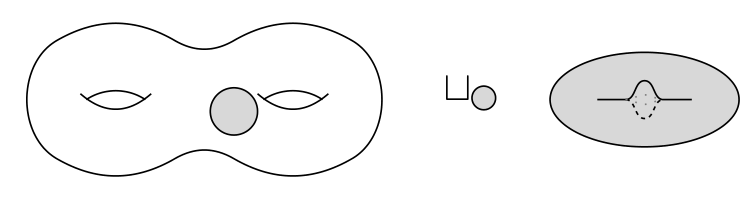
\includegraphics[width=0.22\textwidth]{p175_d4.png}}.
\end{equation}
用 $G$-丛来说，这意味着我们可以写：
\begin{align}
\mathrm{Hecke}_x&=\Bun_G\big(C\sqcup_{C\setminus x}C\big)\tag{10.257}\\
&=\Bun_G(C)\times_{\Bun_G(C\setminus x)}\Bun_G(C)\tag{10.258}\\
&=\Bun_G(C)\times_{\Bun_G(D)}\Big(\Bun_G(D)\times_{\Bun_G(D^{*})}\Bun_G(D)\Big).\tag{10.259}
\end{align}
即：与其把 $\mathrm{Hecke}_x$ 的元素描述为在 $x$ 之外带同构的一对 $G$-丛，我们可以把它们想成沿圆盘 $D$ 作修改的单个丛。

回忆 $\Bun_G(C,x)$ 是带“$x\in C$ 周围某个圆盘上的平凡化”的 $G$-丛空间。于是我们可以把 $\mathrm{Hecke}_x$ 重新写成：$\Bun_G(C,x)$ 与“圆盘上平凡 $G$-丛的所有修改”构成的空间的乘积，再模掉平凡化变换群 $G(\mathcal{O}_x)$：
\begin{equation}\tag{10.260}
\mathrm{Hecke}_x=\big(\Bun_G(C,x)\times\text{modifications}\big)\big/G(\mathcal{O}_x).
\end{equation}
这其实是我们已经见过的东西的一个版本，例如定理~5：
\begin{equation}\tag{10.261}
\Bun_G=G(F_x)\backslash\prod_{x\in C}^{\prime}G(K_x)/\prod_{x\in C}G(\mathcal{O}_x).
\end{equation}
当我们在 $x\in C$ 周围作平凡化时，我们玩同样的游戏，只是不模掉右边的一个因子：
\begin{equation}\tag{10.262}
\Bun_G(C,x)=G(F)\backslash\prod_{y}^{\prime}G(K_y)/\prod_{y\neq x}G(\mathcal{O}_y).
\end{equation}
于是这个空间带有整个圈群 $G(K_x)$ 的作用。所以我们有 $\Bun_G(C)$，它带有群 $G(\mathcal{O}_x)$ 的主丛：
\begin{equation}\tag{10.263}
\begin{array}{c}
\Bun_G(C,x)\\[2pt]
\downarrow{\scriptstyle G(\mathcal{O}_x)}\\[2pt]
\Bun_G(C)
\end{array}
\end{equation}
而全空间有大群 $G(K_x)$ 的作用。换言之，$\Bun_G(C)$ 是 $G(K_x)$-空间对子群 $G(\mathcal{O}_x)\subset G(K_x)$ 的商，而 Hecke 修改一般正是从这里来的。于是我们有：
\begin{equation}\tag{10.264}
\mathrm{Hecke}_x\simeq\big(\Bun_G(C,x)\times G(K_x)/G(\mathcal{O}_x)\big)\big/G(\mathcal{O}_x),
\end{equation}
即这是从主 $G(\mathcal{O})$-丛 $\Bun_G(C,x)$ 出发、在 $\Bun_G$ 上的相伴 $G(K)/G(\mathcal{O})$-丛。

所以我们有：
\begin{equation}\tag{10.265}
\begin{array}{ccc}
\Bun_G(C,x) & \longrightarrow & G(K_x)\\[4pt]
\downarrow{\scriptstyle G(\mathcal{O}_x)} & & \\[4pt]
\Bun_G(C) & &
\end{array}
\end{equation}
这给出 Hecke 群胚的作用：
\begin{align}
G(\mathcal{O}_x)\backslash G(K_x)/G(\mathcal{O}_x)&=\Bun_G\big(D\sqcup_{D\setminus x}D\big)\tag{10.266}\\
&=\text{$D$ 上丛的修改}\tag{10.267}\\
&=\Big\{P_1,P_2\in\Bun_G(D),\ P_1|_{D^{*}}\xrightarrow{\ \sim\ }P_2|_{D^{*}}\Big\}.\tag{10.268}
\end{align}

这一切的结论是如下。在物理图像中
\begin{equation}\tag{10.269}
\mathcal{A}_G\big(S^2\big)=\Shv\big(\Bun_G(S^2)\big)
\end{equation}
被线算子作用。在群论图像中，我们有这个 Hecke 东西的作用，即意大利饺上 $G$-丛的层：
\begin{equation}\tag{10.270}
\Shv\big(G(\mathcal{O})\backslash G(K)/G(\mathcal{O})\big)=
\Shv\Big(\Bun_G\big(\text{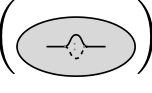
\includegraphics[width=0.07\textwidth]{p177_d1.png}}\big)\Big).
\end{equation}
但想法是：一旦我们给意大利饺填上足够的馅，这两者相距不远。

这就是\term{球 Hecke 范畴}{spherical Hecke category}的定义：
\begin{equation}\tag{10.271}
\Sph:=\Shv\big(G(\mathcal{O})\backslash G(K)/G(\mathcal{O})\big).
\end{equation}
这是几何 Langlands 纲领中的中心对象。它通过 Hecke 算子作用在 $\Shv(\Bun_G C)$ 上。所以我们看到了来自数论的阿黛尔描述，它说 $\Bun_G$ 有很多由对应实现的对称性：它不是群，但它是一个带群作用的空间的商。这正是我们得到这种由 Hecke 算子实现的剩余对称性的时候。然后我们可以把这些 Hecke 算子看成理论的线算子，而线算子是交换的。所以 $\Sph$ 是一个交换张量范畴，尽管 Hecke 代数/范畴一般并不交换。（原稿批注：move example?——此例是否移位待定。）

\begin{srcex}{70}（经典 Hecke 对应）
设 $V$ 是 $C$ 上秩 $n$ 的向量丛，$x\in C$。现在我们要“在 $x$ 处修改 $V$”。最容易的做法是看：
\begin{equation}\tag{10.272}
V(-x)=V\otimes\mathcal{O}(-x)\hookrightarrow V,
\end{equation}
它的截面定义为在 $x$ 处消失的 $V$ 的截面。这是我们在交换情形所做的，即给定线丛，这只是修改相应的除子。

下面是一个更有意思的修改。设 $W$ 是 $V|_x$ 的 $k$ 维子空间。那么我们可以修改 $W$ 得到 $V(-W)$，其截面由在 $x$ 处落在 $W$ 中的 $V$ 的截面给出，即：
\begin{equation}\tag{10.273}
\Gamma\big(V(-W)\big)=\big\{s\in\Gamma(V)\ \big|\ s|_x\in W\subset V|_x\big\}.
\end{equation}
这事实上是向量丛，且是 $V$ 的子丛。

这给出一种在一点处修改向量丛的方法，对任意子空间 $W$ 的选择，即在纤维的 $k$ 维子空间 Grassmann 簇中选一点：
\begin{equation}\tag{10.274}
W\in\Gr_k\big(V|_x\big).
\end{equation}
因此我们有一个对应：
\begin{equation}\tag{10.275}
\begin{array}{ccc}
& \mathrm{Hecke}^{k}_x &\\[4pt]
\swarrow & & \searrow\\[4pt]
\Bun_n(C) & & \Bun_n(C)
\end{array}
\end{equation}
其中
\begin{equation}\tag{10.276}
\mathrm{Hecke}^{k}_x=\text{“}\Gr_k(E|_x)\text{”}=\big\{(V,\,W\in\Gr_k(V|_x))\big\},
\end{equation}
而 $E$ 是万有丛。即这是一个以两种方式成为 $\Bun_n(C)$ 上 Grassmann 丛的对象，定义了上述对应：
\begin{equation}\tag{10.277}
\mathrm{Hecke}^{k}_x\;\rightsquigarrow\;
\big(V,\ W\in\Gr_k(V|_x)\big)\;\rightsquigarrow\;V(-W).
\end{equation}
\end{srcex}
于是 $\Bun_n(C)$ 回到自身的映射并没有那么多（若它是一个群我们可能会期待很多），但它是 $G$-空间的商，所以带有大量有意思的自对应；例如这里对任意非负整数 $k\le n$ 我们都得到一个。这些是基本的 Hecke 修改，它们将生成所有 Hecke 算子的格。

% [Tutor Note: 本节的记号是全书最密的：$F_x$ 是 $x$ 处的局部域、$\mathcal{O}_x$ 是其整数环、$K_x$ 是分式域（“圈群”$G(K_x)$ 即 $G$ 在局部域上的点）；$\prod'$ 表示阿黛尔意义下的受限乘积。(10.261) 中 $\Bun_G$ 与 $\Bun_G(C)$ 混用是原文写法（前者指整体模栈）。(10.262) 原文分母印作 $\prod_{y\ne x}G(\mathcal{O}_x)$，按意义应为 $G(\mathcal{O}_y)$，这是原稿的下标笔误，照译并指出。(10.273) 原文在两个集合之间漏印了关系符号，本译本按意义补为 $=$。最后要记住：几何 Langlands 的“自守侧”是 $\Shv(\Bun_G(C))$，“谱侧”由 Hecke 范畴 $\Sph$ 作用；Hecke 算子就是物理上的线算子，而线算子交换，这正是 $\Sph$ 虽是 Hecke 范畴却交换的原因。]


\chapter{几何 Satake}\label{ch:11}

\begin{keytakeaways}
本章讲述几何 Satake 对应：仿射 Grassmann 流形$\Gr_G=G(K)/G(\cO)$在$LG_+$-等变层下的范畴$\sph$，作为对称幺半范畴，等价于 Langlands 对偶群$G^{\vee}$的表示范畴。技术路线是：先观察到$\Gr_G$的$LG_+$-轨道由余权格$\Lambda$模 Weyl 群标号，再借由抛物限制把$\Gr_G$上的层拉回到$\Gr_T\simeq\Lambda$上的层，从而用 Fourier 级数（Tannakian 重构）读出$G^{\vee}$；几何 Satake 定理正是这一重构的严格化。由此，$\sph$以 Hecke 算子的形式作用在$\Shv(\Bun_G(C))$上，其谱分解给出几何 Langlands 纲领的 Hecke 特征层，并在物理上对应规范理论$A_G$与 4 维 B-模型$B_{G^{\vee}}$的电磁对偶。
\end{keytakeaways}

\section{总体思想}\label{sec:11-1}

\begin{sectionkey}
本节回顾贯穿全书的“群胚作用”图景：一个带$K$-作用的空间$X$给出群胚$X/K\rightrightarrows \mathrm{pt}/K$，并给出 Hecke 对应；平衡积$\times^K$是把$G/K$丛化到$X/K$上的标准工具。
\end{sectionkey}

\begin{flushright}\small 第 26 讲；2021 年 4 月 29 日\end{flushright}

回顾一般图景：当给定$X\supset K$（即$K$作用于$X$）时，我们有一个群胚作用：
\begin{equation}\tag{11.1}
\begin{array}{ccc}
X/K & \quad\circlearrowleft\quad & K\backslash G/K\\[2pt]
 & \searrow\ \swarrow & \\[2pt]
 & \mathrm{pt}/K &
\end{array}
\end{equation}
或者等价地，我们有一个由 Hecke 给出的对应：
\begin{equation}\tag{11.2}
\begin{array}{ccc}
 & \operatorname{Hecke} & \\
 \swarrow & & \searrow\\
 X/K & & X/K
\end{array}
\end{equation}
其中$\operatorname{Hecke}$是$X/K$上由主$K$-丛$X\to X/K$诱导的$G/K$-丛，也就是说，我们把$G/K$看成带$K$-作用的空间，于是有：
\begin{equation}\tag{11.3}
\operatorname{Hecke}=X\times^{K}G/K,
\end{equation}
其中$\times^{K}$表示\term{平衡积}{balanced product}，即我们已经对$X$上$K$的右作用和$G/K$上$K$的左作用作了商。

% [Tutor Note: 原文记号$X\supset K$是“$K$作用在$X$上”的简写，并非包含关系；平衡积$X\times^KG/K$的严格含义是$(X\times G/K)/K$，其中$k\cdot(x,gK)=(xk^{-1},kgK)$。这一约定在 (11.14) 的$LG_+$-丛中反复使用，读者若不熟悉伴随丛的构造，可对照 [Bor91] 或任何主丛教材。]

\section{仿射 Grassmann 流形}\label{sec:11-2}

\begin{sectionkey}
本节定义\term{仿射 Grassmann 流形}{affine Grassmannian} $\Gr_G=G(K)/G(\cO)=LG/LG_+$，把它实现为圆盘上平凡$G$-丛在一点处的修正，并说明其上的$LG_+$-轨道等价于分数维 Hecke 对应的核；最后（11.2.1–11.2.2）讨论它的同伦型$\Omega G_c$与 Bialynicki-Birula 胞腔分解。
\end{sectionkey}

对$x\in C$，我们将构造$\operatorname{Hecke}$的一个版本，称为$\operatorname{Hecke}_x$：
\begin{equation}\tag{11.4}
\begin{array}{ccc}
 & \operatorname{Hecke}_x & \\
 \swarrow & & \searrow\\
 \Bun_G(C) & & \Bun_G(C)
\end{array}
\end{equation}

这是一个纤维化，其纤维由仿射 Grassmann 流形给出：
\begin{align}
\Gr_G&:=G(K_x)/G(\cO_x)\tag{11.5}\\
&=LG/LG_+.\tag{11.6}
\end{align}
我们可以这样看：
\begin{equation}\tag{11.7}
G(K_x)=LG=\operatorname{Map}(D^{*},G),
\end{equation}
而在其中我们有：
\begin{equation}\tag{11.8}
G(K_x)\supset G(\cO_x)=LG_+=\operatorname{Map}(D,G).
\end{equation}
对任意曲线$C$，$\Gr$可以写成：
\begin{align}
\Gr_G&=LG/LG_+\tag{11.9}\\
&=\{\text{$C$上的$G$-丛，且在 }C\setminus x\text{ 上平凡}\}\tag{11.10}\\
&=\{\text{$D$上的$G$-丛，且在 }D\setminus x\text{ 上平凡}\},\tag{11.11}
\end{align}
即它由$D$上平凡丛在点$x$处的修正组成。

我们可以把$\operatorname{Hecke}_x$明确写成三元组的集合：
\begin{align}
\operatorname{Hecke}_x&=\Bigl\{P_1,P_2\in\Bun_G(X),\ P_1|_{C\setminus x}\xrightarrow{\ \sim\ }P_2|_{C\setminus x}\Bigr\}\tag{11.12}\\
&=\Bigl\{P_1,\ P_2|_{D},\ P_1|_{D^{*}}\xrightarrow{\ \sim\ }P_2|_{D^{*}}\Bigr\}.\tag{11.13}
\end{align}
上面的描述清楚地表明我们有两个到$\Bun_G(C)$的映射（一个把三元组送到$P_1$，另一个送到$P_2$），但下面的描述告诉我们，$\operatorname{Hecke}$与$\Bun_G$上的主$LG_+$-丛相关联，该丛由$\Bun_G(C,x)$（在$D_x$上有平凡化的$G$-丛构成的空间）给出。也就是说：
\begin{equation}\tag{11.14}
\operatorname{Hecke}_X=\Bun_G(C,x)\times^{LG_+}\Gr.
\end{equation}
也就是说，我们从$P\in\Bun_G$出发并在$D$上平凡化，于是得到$P$连同平凡化这一对，即$\Bun_G(C,x)$中的对象。然后我们修正$D$上的平凡丛，以在$\Bun_G(C,x)\times\Gr$中得到$P$和$P'$，接着对$G(\cO)=LG_+$取商。

于是$\operatorname{Hecke}_x$以两种方式成为$\Bun_G$上的扭$\Gr$-丛：
\begin{equation}\tag{11.15}
\begin{array}{ccccc}
 & & \operatorname{Hecke}_x & & \\
 & \swarrow & & \searrow & \\
\Bun_G & & & & \Bun_G\\
 & \searrow & & \swarrow & \\
 & & \Gr & &
\end{array}
\end{equation}
例如通过映到$P$或映到$P'$。

这有什么用处？$\operatorname{Hecke}$是一个群胚，因此我们可以尝试用它作用在$\Bun_G$上。确定$\operatorname{Hecke}$中的点并不容易，但我们可以挑出轨道。局部地，一旦选定平凡化，它看起来就像$\Gr\times\Bun_G$。若改变平凡化，则这一识别差一个左作用$LG_+\circlearrowright\Gr$。这其实只是伴随丛的一般事实：$\Gr$上任何$LG_+$-不变的对象在整空间$\operatorname{Hecke}_x$上都有意义。例如若取$\Gr$中任何$LG_+$-轨道$O$，即$O$对应一个陪集$LG_+\backslash LG/LG$，则这给出$\Bun_G$与自身之间的一个对应：
\begin{equation}\tag{11.16}
\begin{array}{ccc}
 & O & \\
 \swarrow & & \searrow\\
 \Bun_G & & \Bun_G
\end{array}
\end{equation}
因此，给定这一个对象$\operatorname{Hecke}_x$，我们应当把它看成给出许多不同的对应，以$\Gr$中的轨道为标号。

\begin{srcex}{71}
回忆在例 70 中我们取$G=GL_n$，并对任意满足$0\le k\le n$的整数$k$得到一个对应：
\begin{equation}\tag{11.17}
\begin{array}{ccccc}
 & & \operatorname{Hecke}_x^{k} & & \\
 & \swarrow & & \searrow & \\
\Bun_n(C) & & & & \Bun_n(C)\\
 & \searrow & & \swarrow & \\
 & & \Gr_k^n & &
\end{array}
\end{equation}
\end{srcex}
这个$\operatorname{Hecke}_x^{k}$就是来自$\Gr$中轨道的对应之一例。事实上，$GL_n(\cO)=L(GL_n)_+$在
\begin{equation}\tag{11.18}
\Gr_{GL_n}=GL_n(K)/GL_n(\cO)
\end{equation}
上的闭轨道与整数$0\le k\le n$一一对应，且同构于通常的 Grassmann 流形$\Gr_k^n$。具体地，$\Gr_{GL_n}$由圆盘$D$上秩为$n$的向量丛$V$连同$D^{*}$上的平凡化组成。我们可以非常具体地写出如下。考虑$V$在圆盘上的正则截面$V(D)$。它位于去心圆盘上的截面空间之内，而后者已被平凡化：
\begin{equation}\tag{11.19}
V(D)\subset V(D^{*})\cong K^{n},
\end{equation}
所以这是$K^{n}$的子空间，即$n$份 Laurent 级数。事实上，这不仅是子空间，还是$K^{n}$的$\cO$-子模。若把参数取逆，我们得到：
\begin{equation}\tag{11.20}
V(D)\otimes_{\cO}K\simeq K^{n}.
\end{equation}
换言之，仿射 Grassmann 流形就是$K^{n}$内所有$\cO$-格的集合。

我们可以用某个$N$来界定极点的阶，于是发现子空间$V(D)$被夹在：
\begin{equation}\tag{11.21}
t^{-N}\cO^{n}\subset V(D)\subset t^{N}\cO^{n}\subset K^{n}.
\end{equation}
这个夹层两端的商是有限维向量空间，因此$V(D)$给出其中一个子空间。它还对坐标乘法封闭。无论如何，它是有限维 Grassmann 流形的一个闭子簇。于是我们得到$\Gr_n$的描述
\begin{equation}\tag{11.22}
\Gr_n=\bigcup_{N}\{\text{射影簇}\}.
\end{equation}
即$\Gr_n$是 ind-真（ind-proper）ind-概形。对其他群，我们可以通过选取到$GL_n$的忠实表示，把相应的$\Gr_G$嵌入$\Gr_n$。对$N=1$，我们可以看到有限维的$\Gr_k^n$作为轨道位于其中。

所以思路是：我们研究$\Gr$，但只想研究在$G(\cO)$作用下不变的几何。任何这样的几何在$\Bun_G$上都有意义。例如我们可以考虑不变层$\Shv^{G(\cO)}(\Gr)$，然后它映到$\Shv(\operatorname{Hecke}_x)$。因此，通过$\operatorname{Hecke}_x$的群胚作用，我们得到$\Bun_G$上的积分核，即有映射：
\begin{equation}\tag{11.23}
\Shv^{G(\cO)}(\Gr)\longrightarrow\Shv(\operatorname{Hecke}_x)\longrightarrow\End\bigl(\Shv(\Bun_G)\bigr).
\end{equation}
再次：
\begin{equation}\tag{11.24}
\Shv^{G(\cO)}(\Gr)=\Shv\bigl(G(\cO)\backslash G(K)/G(\cO)\bigr)=:\sph.
\end{equation}
于是轨道$O$通过考察$O$上常值层在这两个映射下的像给出一个算子。在物理图景中，我们在某点$x\in C$和某时刻$t\in I$插入$O$：
\diageq{11.25}{0.14\textwidth}{p182_d1.png}
结合律来自$\{x\}\times I$上三点构型的结合性。交换律则是因为，给定放置算子的两个这样的点，我们有足够的维数让这些点交换位置。现在我们要从物理中提炼这一想法，以看出这些 Hecke 算子是交换的。关键在于$\Gr$带有某种额外的代数结构，其形式并不十分常见，来源于移动点$x\in C$。

% [Tutor Note: (11.14) 原文写作$\operatorname{Hecke}_X$，而其余各处均为$\operatorname{Hecke}_x$，是记号笔误（$x$为曲线上一点，$X$为曲线/概形），译文保留原式并在此指出。(11.22) 中的并集应理解为$\mathrm{colim}_N$，故只能说$\Gr_n$是 ind-真 ind-概形而非真概形。]

\subsection{$\Gr$的同伦型}\label{sec:11-2-1}

回忆对$G=GL_1$有$\Gr_1=\Z$。我们的 Fourier 级数描述正来源于此。所以$\Gr$是$\Z$的某种推广。按定义，$\Gr$由$\bA^{1}$上的$G$-丛连同$\bA^{1}\setminus 0$上的平凡化组成。若只考虑$\Gr$的同伦型，我们可以把它想成：
\begin{equation}\tag{11.26}
\Gr=\{\text{$\R^{2}$上的$G$-丛}+\text{$\R^{2}\setminus D_0$上的平凡化}\}.
\end{equation}
我们还可以再往前一步，取：
\begin{align}
\Gr&\simeq\{\text{$\R^{2}$上的$G_c$-丛}+\text{$\R^{2}\setminus D_0$上的平凡化}\}\tag{11.27}\\
&\simeq\operatorname{Map}\bigl((\R^{2},\R^{2}\setminus D);(BG,*)\bigr)\tag{11.28}\\
&\simeq\Omega^{2}BG\tag{11.29}\\
&\simeq\Omega G\tag{11.30}\\
&\simeq\Omega G_c,\tag{11.31}
\end{align}
其中$D_0$是围绕原点的圆盘，$G_c\subset G$是极大紧子群。

\begin{srcrem}{71}
这甚至是同胚（即不止是同伦型相同）：$\Omega G_c$与$\Gr$同胚。
\end{srcrem}

因此我们有：
\begin{equation}\tag{11.32}
\pi_0\Gr=\pi_2(BG)=\pi_1(G).
\end{equation}
所以若$G$单连通，则$\Gr$连通，例如$G=SL_n(\C)$单连通，故其$\Gr$连通。更有意思的是，任何空间上的二重基于环路$\Omega^{2}(-)$在 homotopy 意义下是弱交换群。这正是任何空间的$\pi_2$交换的原因。

为了把$\Omega^{2}X$上的“交换”乘法形式化，我们引入小 2-圆盘（little 2-disk，$E_2$）operad。用这些术语，$\Omega^{2}X$是一个$E_2$-空间。考虑圆盘$D$内$k$个圆盘的构型：
\diageq{11.33}{0.16\textwidth}{p183_d1.png}
我们可以把每个小圆盘$\{D_i\}_{i=1}^{k}$标记为一个映射$f_i$，其中
\begin{equation}\tag{11.34}
(f_1,\dots,f_k)\in\bigl(\Omega^{2}X\bigr)^{k}.
\end{equation}
然后我们可以定义一个新的映射，它把小圆盘的补集
\begin{equation}\tag{11.35}
D\setminus\Bigl(\bigsqcup_{i=1}^{k}D_i\Bigr)
\end{equation}
送到基点，并在$D_i$上赋值$f_i$。这定义了一个$k$重乘法映射：
\begin{equation}\tag{11.36}
\operatorname{Conf}_k(D)\times\bigl(\Omega^{2}X\bigr)^{k}\longrightarrow\Omega^{2}X.
\end{equation}
我们可以如 图 11.1 那样复合这些乘法映射。

\begin{figure}[htbp]
  \centering
  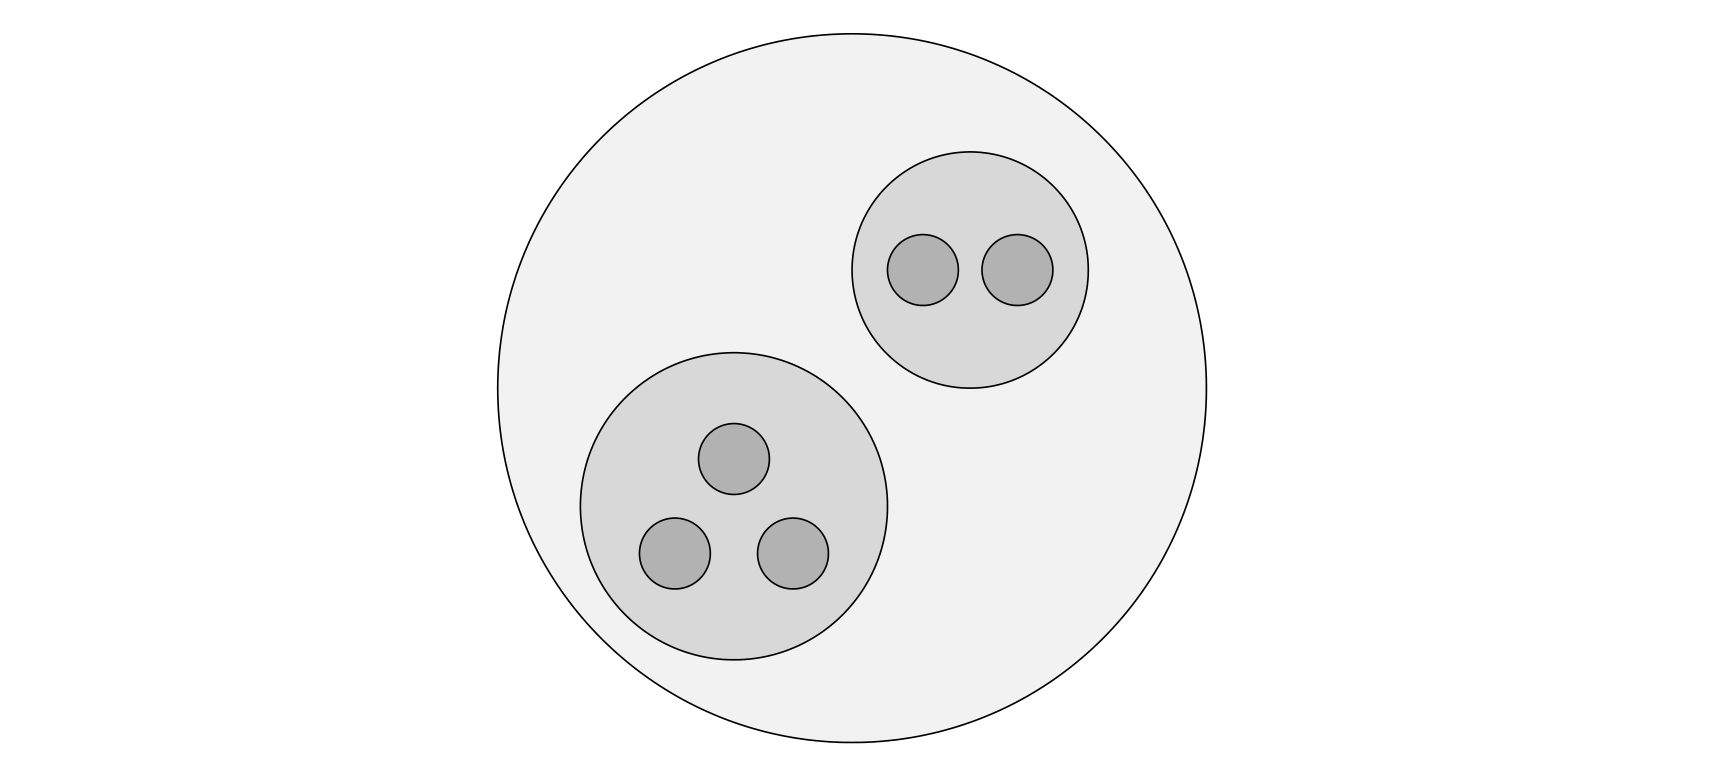
\includegraphics[width=0.42\textwidth]{figure11-1.png}
  \caption{一个二重乘法与一个三重乘法的复合给出一个五重乘法。（原文 p.~184，Figure 11.1）}
  \label{fig:11-1}
\end{figure}

\paragraph{题外话 5.}
应当把这与拓扑中如下论证作类比。对
\begin{equation}\tag{11.37}
f_1,f_2\in\pi_2(X)=\pi_0\bigl(\Omega^{2}X\bigr),
\end{equation}
我们可以想象红色部分被送到基点，并且
\begin{equation*}
\begin{array}{ccc}
\overset{f_1}{\bullet} & \simeq & \overset{f_2}{\bullet}\\[2pt]
 & \simeq & \\
\overset{f_2}{\bullet} & & \overset{f_1}{\bullet}
\end{array}
\end{equation*}
于是$\Gr$是$E_2$-空间。因此当我们把它线性化时，将得到一个$E_2$-对象。例如$\Shv(\Gr)$是$E_2$-范畴：它具有“弱交换”乘法。

\begin{srcrem}{72}
这对应着 3 维场论中线算子构成编织$\otimes$-范畴的方式。编织$\otimes$-范畴的范畴等价于$E_2$-范畴的范畴。
\end{srcrem}

也就是说，$\Gr$在 homotopy 理论的世界里有点像交换群。因此我们可以考虑某种拓扑层，例如局部系统，但我们需要更精细的东西，例如代数几何中会取的层。断言是：$\Gr$在代数几何的世界里也是某种交换群。这就是\term{因子化空间}{factorization space}的概念。

\begin{srcrem}{73}
眼下我们在曲线$C$上移动点，于是得到更大 2-圆盘中 2-圆盘的$E_2$-结构。但我们说过线算子其实更好：它们是$E_3$，因为我们多了一个时间维。然后当我们来到$\Gr$时，我们只看其模$G(\cO)$-作用的部分，即考虑
\begin{equation}\tag{11.38}
G(\cO)\backslash\Gr=G(\cO)\backslash\Gr/G(\cO),
\end{equation}
它实际上是$E_3$-空间，即比$E_2$更好。
\end{srcrem}

\begin{srcrem}{74}（警告）
我们忽略了$\Gr$的非约化结构。若$G$半单，则$\Gr$是约化的。即便是$\Gr_{GL_1}$，实际上也是$\Z\times$某个无穷维形式群。
\end{srcrem}

我们知道：
\begin{align}
\Gr_{GL_1}&=GL_1(K)/GL_1(\cO)\tag{11.39}\\
&=K^{*}/\cO^{*},\tag{11.40}
\end{align}
这里把二者都看成无穷维概形。由此我们应当有切空间
\begin{equation}\tag{11.41}
T\Gr_{GL_1}=\operatorname{Lie}(K^{*})/\operatorname{Lie}(\cO^{*})=K/\cO=\C((t))/\C[[t]],
\end{equation}
这是一个无穷维向量空间。一切交换，故$K/\cO$是无穷维 Lie 代数，于是可以指数化$\exp(K/\cO)$，得到无穷维形式群。于是
\begin{equation}\tag{11.42}
K^{*}/\cO^{*}\simeq\Z\times\exp(K/\cO),
\end{equation}
它大致是$\Z\times\bA^{\infty}$。

即便这对半单的$G$不出现，我们也不能忽略它。回忆$\operatorname{Pic}(C)=H^{1}(C,\cO^{*})$以及
\begin{equation}\tag{11.43}
T\operatorname{Pic}(C)=H^{1}(C,\cO)\simeq\cO(C\setminus x)\backslash K_x/\cO_x
\end{equation}
以及
\begin{equation}\tag{11.44}
K/\cO\twoheadrightarrow\cO(C\setminus x)\backslash K_x/\cO_x.
\end{equation}
于是我们有从$x$处的除子到 Pic 的映射：
\begin{equation}\tag{11.45}
K^{*}/\cO^{*}\to\operatorname{Pic},
\end{equation}
所以我们在$K_x/\cO_x$中忽略掉的多余部分，正是使 Pic 不离散的东西。

% [Tutor Note: (11.42) 中的$\bA^\infty$是形式无穷维仿射空间，原文 OCR 只留下 “$\Z\times$ d”，此处依 p.184 页面图恢复。(11.43) 的$T\operatorname{Pic}(C)=H^1(C,\cO)$是形式切空间，其右侧$\cO(C\setminus x)\backslash K_x/\cO_x$为“在$x$外正则的亚纯函数模去整函数”的商，切勿与$H^1$的 Zariski 切空间混淆。]

\subsection{$\Gr$的几何结构}\label{sec:11-2-2}

好的参考见 [PS86]。

我们首先要考虑的是$\Gr$的 Morse 理论/Bialynicki-Birula 分解/胞腔分解。分解的胞腔由到极大环面的同态标号，这些同态构成余权格：
\begin{equation}\tag{11.46}
\Bigl\{G_m\xrightarrow{\ \phi\ }T\subset G\Bigr\}=\Lambda.
\end{equation}
当我们有$G_m$的作用时便得到这样的分解。首先有来自旋转 Laurent 级数的$G_m\circlearrowright\Gr$。我们也可以在$T$内取一个一般的$G_m$拷贝：
\begin{equation}\tag{11.47}
G_m\xrightarrow{\ \rho^{\vee}\ }T\subset G.
\end{equation}
“一般”意味着中心化子$Z(\rho^{\vee})=T$。于是
\begin{equation}\tag{11.48}
G_m\to T\subset G\subset LG_+
\end{equation}
也作用在$\Gr$上。因此我们可以取对角作用，即同时旋转圆盘并作用这个$G_m$拷贝。

这个组合作用的不动点是什么？我们要找的是在两种作用下都不变的映射$D^{*}\to G\in G(K)$。因此不动点由余特征给出：
\begin{equation}\tag{11.49}
\{\phi\colon G_m\to T\}.
\end{equation}
这些可以限制到$D^{*}\subset G_m$，然后记住$T\subset G$。也就是说，我们有映射
\begin{equation}\tag{11.50}
\{\phi\colon G_m\to T\}\longrightarrow\{\phi\colon D^{*}\to G\},
\end{equation}
即余特征映到$\phi\in G(K)$，然后可以取相应的陪集。

\begin{srcex}{72}
对$GL_n$，我们考虑矩阵
\begin{equation}\tag{11.51}
\begin{pmatrix}
t^{i_1} & & & \\
 & t^{i_2} & & \\
 & & \ddots & \\
 & & & t^{i_n}
\end{pmatrix}\in GL_n(K).
\end{equation}
\end{srcex}
结论是：我们得到$\Gr$的一个胞腔分解，每个胞腔的中心恰有一个不动点。

我们其实已经见过这个余权格$\Lambda$。它是$T$的 Grassmann 流形：
\begin{equation}\tag{11.52}
\Lambda\simeq T(K)/T(\cO)=\Gr_T.
\end{equation}
也就是说：
\begin{equation}\tag{11.53}
\Lambda\cong\Gr_T\hookrightarrow\Gr_G.
\end{equation}
这是把非交换$G$的情形归约到交换$T$的情形的第一步。

下一步是找到 Cartan 分解。这些胞腔（不完全是同一回事，但）包含在$G(\cO)$-轨道之中。$\Gr$中的$G(\cO)$-轨道对应于$\Lambda$的点模 Weyl 群：
\begin{equation}\tag{11.54}
G(\cO)\backslash\Gr=LG_+\backslash LG/LG_+\leftrightarrow\Lambda/W\leftrightarrow\Lambda_+.
\end{equation}
背后还有一个仿射 Weyl 群$W_{\mathrm{Aff}}$，并且
\begin{equation}\tag{11.55}
\Lambda/W=W\backslash W_{\mathrm{Aff}}/W.
\end{equation}

% [Tutor Note: (11.54) 的最后一个双射$\Lambda/W\leftrightarrow\Lambda_+$需要先固定一个支配序（dominant chamber）；$\Lambda_+$指支配余权。$G(\cO)$-轨道与$LG_-$-轨道在$\Gr$上的偏序是相反的（见第 11.3 节与图 11.2），这是理解 (11.68) 中“集合相同但偏序反转”的关键。]

\section{$\Gr$中的轨道}\label{sec:11-3}

\begin{sectionkey}
本节把 Fourier 级数$\Vect^{\Z\text{-gr}}\simeq\Rep(G_m)$重释为$\Shv(\Gr_{GL_1})\simeq\QC(\Loc_{G_m}\PP^1)$，并指出对一般$G$应把左端换成$LG_+\backslash LG/LG_+$；后者作为集合与$\Bun_G(\PP^1)$相同，但闭包偏序相反，这一反差是后面分解定理的几何来源。
\end{sectionkey}

\begin{flushright}\small 第 27 讲；2021 年 5 月 4 日\end{flushright}

几何 Satake 对应是 Fourier 级数理论的非交换对应物。回忆 Fourier 级数理论给出识别
\begin{equation}\tag{11.56}
\Vect^{\Z\text{-gr}}\simeq\Rep(G_m).
\end{equation}
然后我们把左端识别为
\begin{equation}\tag{11.57}
\Vect^{\Z\text{-gr}}\simeq\Shv(\Gr_{GL_1}),
\end{equation}
并把右端识别为
\begin{equation}\tag{11.58}
\Rep(G_m)\simeq\QC(\mathrm{pt}/G_m)\simeq\QC\bigl(\Loc_{G_m}\PP^1\bigr).
\end{equation}
目前我们忽略导出结构，因为一切皆交换。于是 Fourier 级数的重新解释是
\begin{equation}\tag{11.59}
\Shv(\Gr_{GL_1})\simeq\QC\bigl(\Loc_{G_m}\PP^1\bigr),
\end{equation}
而我们要把左端换成关于$G$的仿射 Grassmann 流形的表述：
\begin{equation}\tag{11.60}
\Gr_G=G(K)/G(\cO)=LG/LG_+.
\end{equation}
但我们只关心（其上的层）模$G(\cO)$-作用的情形，即关心轨道：
\begin{align}
G(\cO)\backslash\Gr_G&{}\tag{11.61}\\
&=G(\cO)\backslash G(K)/G(\cO)\tag{11.62}\\
&=LG_+\backslash LG/LG_+.\tag{11.63}
\end{align}
回忆我们在物理中把它看成意大利饺（ravioli）上的$G$-丛空间：
\begin{equation}\tag{11.64}
LG_+\backslash\Gr_G=LG_+\backslash LG/LG_+=\Bun_G\bigl(\text{意大利饺}\bigr).
\end{equation}
我们有
\begin{equation}\tag{11.65}
\Bun_G\bigl(\text{意大利饺}\bigr)=\Bun_G(\PP^1),
\end{equation}
并且可以把$\PP^1$看成一个 2-球面，由圆盘$D$与一份去掉原点的$\bA^1$粘成。于是$LG_+$可以看成圆盘上丛的自同构，但我们还需要模掉$\bA^1$上平凡化的改变，即模掉映射$\bA^1\to G$：
\begin{equation}\tag{11.66}
LG_-=\{\bA^1\to G\}.
\end{equation}
因此
\begin{equation}\tag{11.67}
LG_-\backslash LG/LG_+=\Bun_G(\PP^1).
\end{equation}
于是意大利饺与$\PP^1$在拓扑上看起来非常相似，且意大利饺上丛的同构类与$\PP^1$上丛的同构类一一对应。也就是说，我们有双射
\begin{equation}\tag{11.68}
LG_+\backslash LG/LG_+\leftrightarrow\Lambda/W\leftrightarrow\Bun_G\PP^1,
\end{equation}
其中$\Lambda=\Hom(G_m,T)$是余权格。所以二者作为集合相同，但偏序结构非常不同。$LG_+\circlearrowright\Gr$的轨道在闭包关系下构成一个偏序集。这些轨道都是有限维的，且每个轨道的闭包中只有有限多个轨道。另一方面，$\Bun_G\PP^1$作为集合与之相同，但偏序是反过来的。

\begin{srcex}{73}
让我们考虑$G=GL_2$。第一 Chern 类是映射
\begin{equation}\tag{11.69}
\Bun_{GL_2}(\PP^1)\to\Z.
\end{equation}
例如$\deg(\cO\oplus\cO)=0$，而$\deg(\cO\oplus\cO(1))=1$。$\Bun_{GL_2}(\PP^1)$不连通，其连通分支由度数相同的丛组成，即对每个$n\in\Z$有一个分支。
\end{srcex}

考虑度数为$0$的丛。它等同于$SL_2$-丛：
\begin{equation}\tag{11.70}
\Bun_{SL_2}(\PP^1)=\deg^{-1}(0).
\end{equation}

\begin{figure}[htbp]
  \centering
  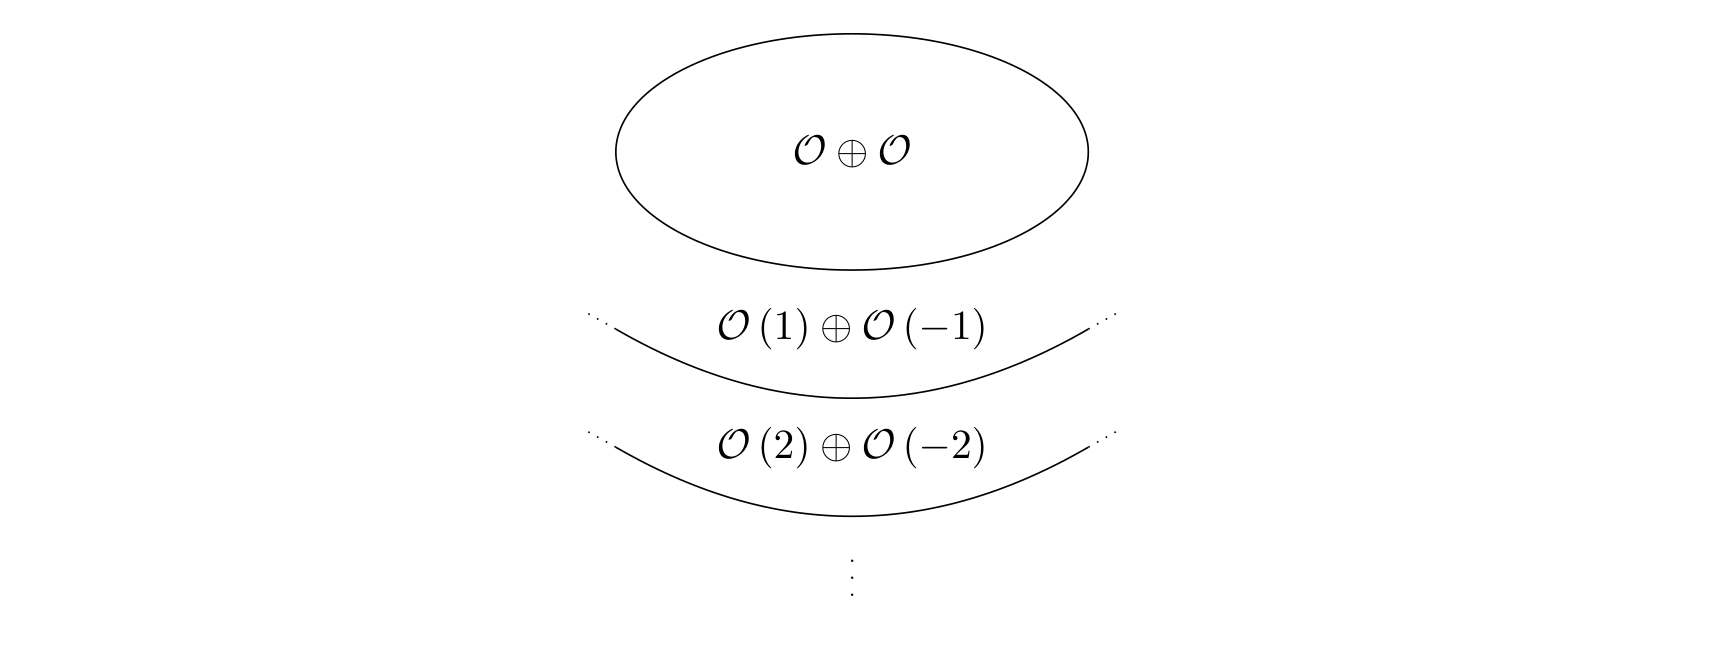
\includegraphics[width=0.5\textwidth]{figure11-2.png}
  \caption{包含平凡丛的$\Bun_{GL_2}(\PP^1)$连通分支有一个开稠密轨道。图中各层对应其他 stratum，它们必然包含在中心开 stratum 的闭包中。我们也可以把此图看作$\Gr$上$LG_-$-轨道的图像。（原文 p.~188，Figure 11.2）}
  \label{fig:11-2}
\end{figure}

这里有平凡丛$\cO\oplus\cO$，以及其他丛如$\cO(1)\oplus\cO(-1)$。这是一个连通空间，含有一个包含$\cO\oplus\cO$的开稠密 stratum。所以所有其他 stratum 都包含在平凡丛所在 stratum 的闭包中。于是偏序看起来像$\mathbb{N}$。

如图 11.2 所示。$\Gr$上的偏序结构是相反的：有一个闭轨道包含在其他一切的闭包之中。

我们也可以把图 11.2 看作$\Gr$中$LG_-$-轨道的图像：有一个开轨道，且所有轨道都是有限余维的。这与$\Gr$中$LG_+$-轨道的情形相反——那里轨道是有限维的，且闭包关系方向相反。

% [Tutor Note: (11.68) 中第二个双射严格地说应写成$LG_+\backslash LG/LG_+\leftrightarrow\Bun_G(\PP^1)$的同构类集合，而非$\Bun_G\PP^1$本身；原文以同一记号兼指模空间与其点集，译文从之。此处的$\Lambda/W$与$LG_-$-轨道的对应关系依赖$LG_-\backslash LG/LG_+$的分解，与$LG_+$-轨道的$\Lambda_+$标号相差一个支配序取反。]

\section{$\Gr$上的等变层}\label{sec:11-4}

\begin{sectionkey}
本节引入核心范畴$\sph=\Shv_{LG_+}(\Gr_G)$：它是半单的，简单对象由$\Lambda/W$标号；其上同时有来自双陪集的结合乘法和来自因子化的编织乘法，二者经 Eckmann–Hilton 论证合成对称幺半结构。
\end{sectionkey}

在$\Gr_G$内部我们有余权格
\begin{equation}\tag{11.71}
\Lambda\simeq\Gr_T\subset\Gr_G,
\end{equation}
它作为“胞腔中心”坐落，即作为$G_m$-作用的不动点。再次，$LG_+\backslash\Gr_G$与$\Lambda/W$一一对应。而$\Lambda/W$看起来像是某个群$G^{\vee}$的不可约表示，该群的极大环面$T^{\vee}$对偶于$T$，也就是说
\begin{equation}\tag{11.72}
\Lambda=\Hom(T^{\vee},G_m).
\end{equation}
我们将从$\Gr_G$上的$LG_+$-等变层出发（用 Tannakian 方法）重构这个对偶群$G^{\vee}$：
\begin{equation}\tag{11.73}
\sph=\Shv_{LG_+}(\Gr_G).
\end{equation}
这里的$\Shv$指 D-模的阿贝尔范畴，或所谓的反常层（perverse sheaf）范畴。想法是：在每个轨道上，这些层将是带平坦联络的向量丛，或等价地，是平移了轨道维数后的局部系统。

这两类范畴都有简单对象，它们与轨道上的不可约局部系统一一对应。$LG_+$-轨道并不完全是胞腔，但被胞腔铺砌（paved）。特别地，所有$LG_+$-轨道都是单连通的。事实上我们可以把它们显式地描述为$G$的部分旗流形上的仿射丛。这意味着$\sph$中的简单对象与轨道$\Lambda/W$一一对应。

结果是：$\sph$是半单范畴，即每个对象都是单对象的直和。这与维数的奇偶性有关，即各轨道复维数的奇偶性在每个连通分支上为常数。要点在于，这限制了一个轨道上的层与其闭包中轨道上的层之间可能的交互：闭包中的轨道与之相差复余维$2$。这意味着不存在可能的扩张，即对不同轨道上的层有$\operatorname{Ext}^{1}=0$。

结论是：这个范畴非常简单，每个对象都是按轨道标号的对象之直和，即作为抽象范畴有
\begin{equation}\tag{11.74}
\sph\simeq\Vect(\Lambda/W).
\end{equation}
\footnote{识别$\sph\simeq\Vect(\Lambda/W)$并不是一个自然的识别。特别地，$\sph$是幺半的，而$\Vect(\Lambda/W)$在幺半结构意义下是一个糟糕的模型。}
这很好，因为这正是一个约化群的表示范畴的样子。

回忆紧群在 Pontryagin 对偶下对偶于离散群。当我们讨论 Tannakian 版本时，我们看到约化群对偶于半单范畴。所以这种对偶暗示：当我们有某种离散性/半单性时，对偶一侧将涉及某个复约化群之类的东西。

主要的结构是：$\sph$是对称幺半范畴，即它有交换张量积。我们从线算子的角度解释了这一点。这有两种不同的结构，它们以某种精确的方式相容。第一种是来自双陪集上层的结构：
\begin{equation}\tag{11.75}
\Shv(LG_+\backslash LG/LG_+).
\end{equation}
双陪集空间上的层总有一个结合乘法。

还有另一种结构，它类似于编织乘法，来源完全不同。特别地，我们看到$\Gr_G$在取商之前就有乘法结构。也就是说，在同伦意义下
\begin{equation}\tag{11.76}
\Gr_G=\Omega^{2}(BG),
\end{equation}
这赋予它弱交换乘法。在代数几何中我们必须换一种说法，用到 Beilinson–Drinfeld 的因子化概念。

\subsection{因子化结构}\label{sec:11-4-1}

$\Gr_G$有某种阿黛尔版本，它是$\Omega^{2}(BG)$上$E_2$-结构的代数几何版本。随后 Beilinson–Drinfeld 引入了 BD Grassmann 流形。想法是：Grassmann 流形相互拼合的方式编码了某种乘法结构。

固定一条曲线$C$（例如$C=\bA^1,\PP^1$，或任取\footnote{曲线不影响最终答案。}）。然后我们将对所有的$n$定义生活在$C^{n}$上的对象$\Gr_{G,C^{n}}$：
\begin{equation}\tag{11.77}
\begin{array}{ccc}
\Gr_{G,C^{n}} & & \\
\downarrow & & \\
C^{n} & &
\end{array}
\end{equation}
如下所述。对$n=1$这是
\begin{equation}\tag{11.78}
\begin{array}{ccc}
\Gr_{G,C} & & \\
\downarrow & & \\
C & &
\end{array}
\end{equation}
其中$x\in C$上的纤维由$C$上的$G$-丛连同$C\setminus x$上的平凡化构成。于是我们有$\Gr$的这个解释：在原点之外有平凡化的丛。接着 Beilinson–Drinfeld 让原点取任意点$x$，最终得到$C$上的这个丛。$\Gr_{G,C}$是$\Gr_G$上由圆盘上平凡化的改变作用所给出的伴随丛：$\Aut(D)\circlearrowright\Gr_G$。

对$n=2$，
\begin{equation}\tag{11.79}
\begin{array}{ccc}
\Gr_{G,C^{2}} & & \\
\downarrow & & \\
C^{2} & &
\end{array}
\end{equation}
$(x,y)\in C^{2}$上的纤维由$C$上的$G$-丛连同$C\setminus\{x,y\}$上的平凡化构成。注意，尽管$(x,y)$是有序对，该构造在对称群作用下不变。真正有趣的是$C^{2}$中有两个 stratum。我们有开 stratum
\begin{equation}\tag{11.80}
C^{2}\setminus\Delta=\{x\ne y\},
\end{equation}
在它上面
\begin{equation}\tag{11.81}
\Gr_{G,C^{2}}\big|_{x,y}\simeq\Gr_{G,C}\big|_{x}\times\Gr_{G,C}\big|_{y},
\end{equation}
于是有
\begin{equation}\tag{11.82}
\Gr_{G,C^{2}}\big|_{C^{2}\setminus\Delta}\simeq\Gr_{G,C}\big|^{\times 2}_{C^{2}\setminus\Delta}.
\end{equation}
若我们看另一个 stratum
\begin{equation}\tag{11.83}
\{x=y\}=\Delta\subset C^{2},
\end{equation}
则
\begin{equation}\tag{11.84}
\Gr_{G,C^{2}}\big|_{x,y}\simeq\Gr_{G,C}\big|_{x},
\end{equation}
于是
\begin{equation}\tag{11.85}
\Gr_{G,C^{2}}\big|_{\Delta}\simeq\Gr_{G,C}.
\end{equation}

\begin{srcex}{74}
对$G=GL_1$，我们在对角线之外有$\Z\times\Z$，在对角线上有$\Z$。也就是说，我们有$\Z\times\Z\times C^{2}\setminus\Delta$与对角线上的$\Z\times C$粘在一起。粘合映射就是整数的群律。
\end{srcex}

我们可以把这看成群的动态写法。给定两个群元素$(n,m)\in\Z\times\Z$，我们可能想知道它们如何相加。于是我们考虑把$n$放在点$x$，把$m$放在点$y$，并让这两点碰撞。那么$\Gr_{GL_1,C^{n}}$的几何就编码了加法律。也就是说，群结构由$\Z\times\Z$（对角线之外）与$\Z$（对角线上）之间的粘合映射显式呈现。

所以一般而言我们有这个族$\Gr_{G,C^{n}}$，它具有以下两个关键结构。

\begin{enumerate}
\item $\Gr_{G,C^{n}}\big|_{\{x_i\}_{i=1}^{n}}$只依赖于子集$\{x_i\}\subset C$。即对有限集的满射$I\twoheadrightarrow J$我们得到相应的对角映射$\Delta_{I\twoheadrightarrow J}$，并且
\begin{equation}\tag{11.86}
\Delta^{*}_{I\twoheadrightarrow J}\Gr_{C}^{I}\simeq\Gr_{C}^{J}.
\end{equation}
例如$\Delta^{*}\Gr_{C}^{2}\simeq\Gr_{C}$。我们可以换一种说法：$\Gr_{C}(-)$定义了某个有限子集空间上的族，该空间称为$C$的 Ran 空间：
\begin{equation}\tag{11.87}
\operatorname{Ran}(C)=\operatorname{colim}_{I\twoheadrightarrow J}C^{I},
\end{equation}
即$C$的有限子集的参数空间。

\item 因子化：$\Gr$关于不交并运算是乘性的。即
\begin{equation}\tag{11.88}
\Gr_{G,C^{m+n}}\big|_{\{x_i\}_{i=1}^{m}\sqcup\{y_i\}_{i=1}^{n}}\simeq\Gr_{G,C^{m}}\big|_{\{x_i\}_{i=1}^{m}}\times\Gr_{G,C^{n}}\big|_{\{y_i\}_{i=1}^{n}}.
\end{equation}
\end{enumerate}

\begin{srcrem}{75}
在拓扑中我们有一个真正的乘法映射：对从带点圆盘到$BG$的两个映射，我们可以把它们看作生活在更大的圆盘中。现在我们有例如$C$中的两个点，并且可以取它们碰撞的极限。结果来自两份 Grassmann 流形（在$\Delta$之外）与一份 Grassmann 流形（沿$\Delta$）之间的粘合。
\end{srcrem}

这就是所谓的因子化空间。它编码了$\Gr$上不寻常的代数结构，该结构在 homotopy 范畴中退化为$E_2$-结构。它定义了$\Gr$上对象（例如层等）的乘法，我们可以取极限。例如，给定$\cF,\cG\in\Shv(\Gr_G)$以及$x,y\in C=\bA^1$，我们可以认为$\cF$生活在$x$处、$\cG$生活在$y$处：
\begin{equation}\tag{11.89}
\cF\in\Shv\bigl(\Gr_{G,C}|_{x}\bigr),\qquad \cG\in\Shv\bigl(\Gr_{G,C}|_{y}\bigr),
\end{equation}
这定义了一个层
\begin{equation}\tag{11.90}
\cF\boxtimes\cG\in\Shv\Bigl(\Gr_{G,C^{2}}\big|_{C^{2}\setminus\Delta}\Bigr).
\end{equation}
现在我们要取$x\to y$的极限，即要把这个构造延拓到对角线上。若这些层是例如凝聚层，我们就做不到这一点。但若这些层足够接近拓扑层，那就走运了：构造邻近循环（nearby cycles）正是这种极限的拓扑版本。于是我们可以把$\cF*\cG$定义为$\cF\boxtimes\cG$在$\Delta\subset C^{2}$上的邻近循环。

因此$\Shv(\Gr)$大致看起来像$E_2$/编织$\otimes$-范畴，但邻近循环的构造并不恰好给出结合的张量积。然而，若我们限制到$\Gr$上的$LG_+$-等变层，就得到
\begin{equation}\tag{11.91}
\sph=\Shv_{LG_+}(\Gr)
\end{equation}
上的结合、编织张量结构。

我们可以这样理解。我们可以“竖直地”堆叠修正（这是 Hecke 结构），也可以在不同点处作修正并把它们碰撞。于是有三个乘法方向：结合的竖直方向，以及来自碰撞的编织乘法。由 Eckmann–Hilton 论证，这定义了一个交换乘法，即范畴上的对称幺半结构。我们在物理中已经见过这一点：我们研究的是余维$1$缺陷，即$C\times I$中的点，而来自碰撞点/把小球碰进大 3-球所得的乘法是交换的，因为我们有足够的维数让它们互相绕行。

% [Tutor Note: (11.74) 的半单性依赖于系数域特征为$0$（D-模范畴）或$\Q_\ell$-层、且轨道维数奇偶性恒定；若在正特征或整系数下，$\operatorname{Ext}^1$未必消失。(11.88) 的因子化同构必须在$\{x_i\}\cap\{y_i\}=\varnothing$时陈述；在对角线附近应改为邻近循环/因子化范畴的陈述，这正是原文随后讨论的内容。]

\section{$\sph$的 Tannakian 重构}\label{sec:11-5}

\begin{sectionkey}
本节说明如何用 Tannakian 形式重构$G^{\vee}$：先构造$\sph\to\Shv(\Gr_T)\simeq\Rep(T^{\vee})$，再对$\Vect$取纤维函子；并指出$\Spec(\sph)$自然接收$\mathrm{pt}/T^{\vee}\to\Spec(\sph)$。
\end{sectionkey}

回忆 Tannakian 重构从一个对称幺半范畴$(\cC,*)$出发。然后我们给它配上叠$\Spec(\cC,*)$。对足够好的$\cC$，想法是
\begin{equation}\tag{11.92}
\cC\simeq\QC(\Spec(\cC,*)).
\end{equation}
还有一个（可能更熟悉的）变体，其中我们多带一点数据。若我们有$(\cC,*)$连同一个纤维函子（忠实且正合的$\otimes$-函子）
\begin{equation}\tag{11.93}
(\cC,*)\to(\Vect_k,\otimes),
\end{equation}
则这给出一个映射
\begin{equation}\tag{11.94}
\Spec(\Vect_k,\otimes)=\Spec(k)\longrightarrow\Spec(\cC,*),
\end{equation}
它是平坦覆盖。这意味着
\begin{equation}\tag{11.95}
\Spec(\cC,*)\xrightarrow{\ \simeq\ }\mathrm{pt}/\Gal(\cC,F),
\end{equation}
其中
\begin{equation}\tag{11.96}
\Gal(\cC,F)=\Aut(F).
\end{equation}
所以在我们这里需要某个遗忘函子
\begin{equation}\tag{11.97}
\sph=\Shv_{LG_+}(\Gr)\to\Vect.
\end{equation}
说明这一点最简短但也许最缺乏洞见的说法是：这就是上同调函子。我们将采取不同的途径。首先考虑函子
\begin{equation}\tag{11.98}
\sph=\Shv_{LG_+}(\Gr_G)\to\Shv(\Gr_T).
\end{equation}
这很有用，因为
\begin{equation}\tag{11.99}
\Gr_T\simeq\Lambda,
\end{equation}
于是我们直接做 Fourier 级数：
\begin{equation}\tag{11.100}
\Shv(\Gr_T)\simeq\Shv(\Lambda)\simeq\Rep(T^{\vee}),
\end{equation}
其中$T^{\vee}=\Hom(\Lambda,G_m)$。所以通过把$\Gr_G$与$\Gr_T$联系起来，我们将得到一个不只到$\Vect_k$的函子，而是
\begin{equation}\tag{11.101}
\sph\to\Rep(T^{\vee}).
\end{equation}
我们如何把$\Gr_G$与$\Gr_T\simeq\Lambda$联系起来？在 Grassmann 流形内部有$G_m$-作用的不动点：
\begin{equation}\tag{11.102}
\Lambda\hookrightarrow\Gr_G.
\end{equation}
于是我们想把$\Gr_G$上的层对应为对$\Lambda$的每个点附一个向量空间，即对每个胞腔中心的不动点附一个向量空间。

我们接下来会讨论抛物限制，但要点是：我们可以通过穿过$\Gr_B$把$\Gr_G$上的层与$\Gr_T\simeq\Lambda$上的层联系起来：
\begin{equation}\tag{11.103}
\begin{array}{ccc}
 & \Gr_B & \\
 \swarrow & & \searrow\\
 \Gr_G & & \Gr_T
\end{array}
\end{equation}
其中$B$是 Borel：
\begin{equation}\tag{11.104}
G\supset B\twoheadrightarrow T.
\end{equation}
\begin{srcex}{75}
若$G=GL_n$，则$B$由上三角矩阵组成。于是对角矩阵组成$T$，它由$B$模严格上三角矩阵的商给出。
\end{srcex}
于是我们得到一个漂亮的忠实$\otimes$-函子$\sph\to\Rep(T^{\vee})$，它可以限制到$\Vect_k$得到忠实的$\otimes$-函子：
\begin{equation}\tag{11.105}
\begin{array}{ccc}
 & \sph & \\
 \swarrow & & \searrow\\
\Rep(T^{\vee}) & \xrightarrow{\ \operatorname{Forget}\ } & \Vect_k
\end{array}
\end{equation}
但最终，这幅图景将告诉我们：事实上$\Spec(\sph)$自然地接收一个映射
\begin{equation}\tag{11.106}
\mathrm{pt}/T^{\vee}\longrightarrow\Spec(\sph).
\end{equation}

% [Tutor Note: (11.95) 中的箭头方向是$\Spec(\cC,*)\simeq\mathrm{pt}/\Gal(\cC,F)$，即把 Tannakian 叠实现为“纤维函子的自同构群”的分类空间；原文排版把$\simeq$与箭头叠在一起，译文按语义写成$\xrightarrow{\simeq}$。(11.100) 的$\Shv(\Lambda)\simeq\Rep(T^{\vee})$是 Fourier 变换（每点取纤维再对格作 Fourier），需要$\Lambda$为有限生成自由交换群。]

\section{抛物诱导/抛物限制}\label{sec:11-6}

\begin{sectionkey}
本节把最高权理论几何化：用对应$\mathrm{pt}/B\rightleftarrows\mathrm{pt}/G,\mathrm{pt}/T$定义抛物限制（取$N$-不变量）与抛物诱导（$G/B$上截面），并把它搬到$\Gr_B\to\Gr_G,\Gr_T\simeq\Lambda$上，得到 Mirkovi\'c–Vilonen 半无限轨道与几何 Satake 的纤维函子。
\end{sectionkey}

\begin{flushright}\small 第 28 讲；2021 年 5 月 6 日\end{flushright}

\subsection{对约化群}\label{sec:11-6-1}

我们想要一种有意义的方式，把复约化群$G$的表示与极大环面$T$的表示联系起来。这是最高权理论的一个版本。回忆我们可以用最高权理论研究$G$的有限维表示。回顾如下。固定一个 Borel $B\subset G$，即子群$B\subset G$使得$G/B$是$G$的极大射影商。\footnote{等价地，Borel 可定义为$G$的极大 Zariski 闭、连通的可解代数子群。}这个商$\cB=G/B$是$G$的旗簇。在$B$内部我们可以考虑换位子群
\begin{equation}\tag{11.107}
N:=[B,B]\subset B,
\end{equation}
然后取商，得到一个环面：
\begin{equation}\tag{11.108}
T=B/N.
\end{equation}

\begin{srcex}{76}
若$G=GL_n$，则$B$由上三角矩阵组成，$N$由严格上三角矩阵组成，而$T=B/N$由对角矩阵组成。
\end{srcex}

\begin{srcrem}{76}
人们最初可能把环面$T$当作$G$的子群来认识，但更有用的想法是把它看成一个商：
\begin{equation}\tag{11.109}
G\supset B\twoheadrightarrow T.
\end{equation}
\end{srcrem}

现在我们可以构造$\mathrm{pt}/B$，它定义一个对应：
\begin{equation}\tag{11.110}
\begin{array}{ccc}
 & \mathrm{pt}/B & \\
 \swarrow & & \searrow\\
 \mathrm{pt}/G & & \mathrm{pt}/T
\end{array}
\end{equation}
它通过推-拉（push-pull）定义了$\mathrm{pt}/G$与$\mathrm{pt}/T$的线性化（即$G$与$T$的表示）之间的态射。具体地，对$V\in\Rep(G)$，我们可以把它拉回到$\mathrm{pt}/B$得到
\begin{equation}\tag{11.111}
V|_{B}\in\Rep(B).
\end{equation}
然后我们可以把它前推到$\mathrm{pt}/T$。为了看清这是什么，让我们把图景稍微丰富一下，取映射$\mathrm{pt}/B\to\mathrm{pt}/T\leftarrow\mathrm{pt}$的纤维积，得到
\begin{equation}\tag{11.112}
\begin{array}{ccc}
\mathrm{pt}/N & \longrightarrow & \mathrm{pt}/B\\
\downarrow & & \downarrow\\
\mathrm{pt} & \longrightarrow & \mathrm{pt}/T
\end{array}
\end{equation}
因此，从$\mathrm{pt}/B$前推到$\mathrm{pt}/T$，在底层向量空间层面就是从$\mathrm{pt}/N$前推到$\mathrm{pt}$，即取$N$-不变量。于是从$V\in\Rep(G)$出发得到
\begin{equation}\tag{11.113}
\bigl(V|_{B}\bigr)^{N}\in\Rep(T).
\end{equation}
对表示$V$取$N$-不变量给出经典意义上的$V$的最高权向量。$T$的作用就是最高权。

这称为\term{抛物限制}{parabolic restriction}。

注意，这不是从$G$到$T\subset G$的朴素限制，而是把$T$看成$B$的商，并用$\mathrm{pt}/B$作为对应把它们联系起来。它有一个伴随，称为\term{抛物诱导}{parabolic induction}，把一个$T$-表示变成一个$G$-表示，如下所述。

注意映射$\mathrm{pt}/B\to\mathrm{pt}/G$的纤维是旗簇$G/B$。设$C_\lambda$是$T$按某特征$\lambda$作用的一维向量空间。当把它拉回到$\mathrm{pt}/B$时，我们得到
\begin{equation}\tag{11.114}
\mathrm{pt}/B=G\backslash G/B
\end{equation}
上的层，于是$\mathrm{pt}/G$上的层等价于$G/B$上的$G$-等变向量丛$L_\lambda$。然后前推得到
\begin{equation}\tag{11.115}
\Gamma(G/B,L_\lambda)\in\Rep(G).
\end{equation}
这就是最高权表示的经典构造。

\begin{srcrem}{77}
我们可以更抽象地思考这幅图。以$G$为规范群的规范理论是关于映入$\mathrm{pt}/G$的映射的理论，即关于任意空间上$G$-丛的理论。研究$G$-丛时，自然要找约化到$B$（即旗）的约化，然后看相应的$T$-丛。于是这把$G$-丛的理论与$T$-丛的理论联系了起来。我们最终会把它解释为$G$-规范理论与$T$-规范理论之间的一个界面。
\end{srcrem}

现在我们可能想知道，若先做抛物诱导再做抛物限制会怎样，即这一程序给出$\mathrm{pt}/T$的线性化的哪些对称性。复合这些对应，我们看到作为对称性作用的自然对象是纤维积$B\backslash G/B$：
\begin{equation}\tag{11.116}
\begin{array}{ccc}
B\backslash G/B & \longrightarrow & \mathrm{pt}/B\\
\downarrow & & \downarrow\\
\mathrm{pt}/B & \longrightarrow & \mathrm{pt}/G
\end{array}
\end{equation}
即它是 Bruhat 胞腔，集合论上与 Weyl 群一一对应。因此这幅抛物诱导图景的对称性由有限 Hecke 代数给出。

\subsection{对$\Gr_G$}\label{sec:11-6-2}

做这一切的目的是把$G$-规范理论与我们已理解的东西联系起来。思路是：为了研究$\Gr_G$上的层，我们应试着把它们与$\Gr_T$上的层联系起来。

我们已经看到$\Gr_T$是一个格，$\Gr_T\simeq\Lambda$，而且事实上$\Gr_T\simeq\Lambda\hookrightarrow\Gr_G$。但我们不应只作朴素限制。

\begin{srcrem}{78}
除非另有说明，当你试图把$G$与$T$作比较时，应始终使用抛物限制，而不是朴素限制。
\end{srcrem}

基本想法是，我们将有
\begin{equation}\tag{11.117}
\begin{array}{ccc}
 & \Gr_B & \\
 p\swarrow & & \searrow q\\
 \Gr_G & & \Gr_T\simeq\Lambda
\end{array}
\end{equation}
而我们要的基本函子将形如
\begin{equation}\tag{11.118}
q_{*}p^{!}\colon\sph_G\to\sph_T\simeq\Rep(T^{\vee}).
\end{equation}

\subsection{$\Gr_B$}\label{sec:11-6-3}

我们已经看到$\Gr_T$只是一个格，随后又讨论了$\Gr_G$的结构。现在我们来理解$\Gr_B$。这将与约化群情形非常不同，因为$B$可解。按定义
\begin{equation}\tag{11.119}
\Gr_B=B(K)/B(\cO).
\end{equation}
例如我们看的是 Laurent 级数中的上三角矩阵模去 Taylor 级数中的上三角矩阵。我们真正感兴趣的是双陪集栈
\begin{equation}\tag{11.120}
\Gr_B:=B(\cO)\backslash\Gr_B=B(\cO)\backslash B(K)/B(\cO).
\end{equation}
回忆$\Gr_G$由$C\setminus\mathrm{pt}$上有平凡化的$G$-丛组成。$\Gr_B$类似地由$C\setminus\mathrm{pt}$上有平凡化的$B$-丛组成。关键的观察是：$G$-丛的平凡化比把结构群约化到$B$要强得多。要点在于，约化到$B$是给一个完整旗，而若你有平凡化，你就可以直接把坐标子空间取作旗。因此，给定在一点之外有平凡化的$G$-丛，它当然在点之外有到$B$的约化。也就是说，我们得到一个从$C\setminus\mathrm{pt}$到参数化$\C^{n}$中旗的空间的映射，即一个映射$C\setminus\mathrm{pt}\to G/B$。

于是对$P\in\Gr_G$，我们得到$C\setminus\mathrm{pt}$上伴随$G/B$-丛$P\times^{G}G/B$的一个截面。现在我们有一个美妙的东西，称为真性的赋值判别法（valuative criterion of properness），它说：若我有一个从去心曲线出发的映射$D^{*}\to G/B$，则它唯一地延拓为整个圆盘上的映射$D\to G/B$。注意这不是族中的陈述，而是域上的陈述。

所以断言如下。

\begin{srcclaim}{2}
在$k$-点层面，$\Gr_B\to\Gr_G$是双射。
\end{srcclaim}

这不是族中的陈述，即这并非说这些空间不同胚。事实上我们可以如下实现它。无论$\Gr_B$是什么，它都映到$\Gr_G$和$\Gr_T$，而后者完全不连通（$\Gr_T\simeq\Lambda$）。因此
\begin{equation}\tag{11.121}
\Gr_B=\bigsqcup_{\lambda\in\Lambda}\Gr_{B,\lambda},
\end{equation}
即我们把$\Gr_B$撕成了以$\lambda\in\Lambda$标号的块。

图景如下。回忆$\Gr_G$上有$G(\cO)$-轨道，其中包含对应于$\Lambda$中点的$G(\cO)$-不动点。于是，集合论上$\Gr_G$是以$\lambda\in\Lambda$标号的块$S_\lambda$的不交并，$S_\lambda$是$\lambda\in\Lambda$在$\Gr_G$中的原像。再次，由于$T=B/N$，我们有
\begin{equation}\tag{11.122}
\begin{array}{ccc}
\mathrm{pt}/N & \longrightarrow & \mathrm{pt}/B\\
\downarrow & & \downarrow\\
\mathrm{pt} & \longrightarrow & \mathrm{pt}/T
\end{array}
\end{equation}

\paragraph{习题 3.}
用此证明$S_\lambda$恰好是$LN=N(K)$的轨道。

这些轨道称为\term{半无限轨道}{semi-infinite orbits}。这些轨道是无穷维的，但同时也是无穷余维的。

% [Tutor Note: Claim 2 只在$k$-点（甚至只在代数闭域的点）上成立；$\Gr_B\to\Gr_G$在族中既非单射也非满射，因此不能据此断言二者作为 ind-概形同构。习题 3 中$N(K)$的轨道$S_\lambda$与$G(\cO)$-轨道方向相反：前者无穷维、有限维截面的余维无穷，这正是 MV 循环的支撑。]

\subsection{几何 Satake 定理}\label{sec:11-6-4}

以上全部内容的结论是，我们有一个函子
\begin{equation}\tag{11.123}
\sph_T\simeq\Rep(T^{\vee})\xleftarrow{\ \text{对 }N(K)\text{-轨道的 }!\text{-限制的上同调}\ }\sph_G.
\end{equation}
也就是说，我们从$G\in\sph_G$出发，结果是一个$\Lambda$-分次向量空间。我们可以就此打住，也可以与$\operatorname{Forget}\colon\Rep(T^{\vee})\to\Vect$复合，得到一个真正的纤维函子。这就是几何 Satake 对应的正确纤维函子。

它显然是张量函子，因为我们用来构造它的运算都与因子化结构（碰撞点）以及由双陪集实现的对称性相容。它也（相当）显然是忠实的。想法是：我们考虑层$\cF\in\Shv(G(\cO)\backslash\Gr)$，该层支撑在某个 stratum 的闭包上。在这个极大轨道内部选一个不动点$\lambda$；若我们通过限制到$S_\lambda$来做这个测量，则基本得到该点处的 stalk。

在较低的 stratum 上测量会更复杂，但我们至少可以挑出$\cF$支撑的顶维部分，并用它来检验函子是忠实的。

于是我们得到几何 Satake 定理。$\Gr$拓扑中的基本几何现象由 Lusztig 识别，Ginzburg 把它表述成今天的形式（并勾画了证明），随后 Drinfeld 引入了因子化图景，最后 Mirkovi\'c–Vilonen 引入了这些半无限胞腔并完成了证明。（原文此处附引用标记。）

\begin{srcthm}{9}（几何 Satake）
$\sph_G$等价于$\Rep(G^{\vee})$（其中$G^{\vee}$由纤维函子的$\Aut$给出），这里$G^{\vee}$是 Langlands 对偶群。
\end{srcthm}

$G^{\vee}$是一个约化代数群，其极大环面$T^{\vee}\subset G^{\vee}$对偶于$T\subset G$。按我们构造对偶群的方式，它自带一个典范环面。它有相同的 Weyl 群：$W_{G^{\vee}}=W_G$，而且事实上$G$的根数据对偶于$G^{\vee}$的根数据。

$G^{\vee}$的中心等同于$G$的基本群的 Cartier 对偶：
\begin{equation}\tag{11.124}
Z(G^{\vee})\simeq\pi_1(G)^{\vee}=\pi_0(\Gr)^{\vee}.
\end{equation}
\begin{srcex}{77}
$Z(GL_n)=G_m$，它 Cartier 对偶于$\Z=\pi_1(GL_n)$。这与$GL_n$是自 Langlands 对偶的事实一致：$(GL_n)^{\vee}=GL_n$。
\end{srcex}
这些特征显式地决定了对偶群，但它并不只是一个抽象地给出的群：它由$\sph_G$上的 Tannakian 重构显式给出。

\begin{srcrem}{79}
构造$G^{\vee}$所用的环/域就是我们层的系数环/域。这一切本来也可以在$\Z$上而不是$\C$上完成。
\end{srcrem}

\begin{srcrem}{80}
该定理说$\sph_G\simeq\Rep(G^{\vee})$。按我们一直以来的呈现方式，信息通常是从左流向右，即从$\Rep(G^{\vee})$流向$\sph_G$。在模表示理论中，信息沿反方向流动。这算是附带的好处，但我们本来也应期待如此：这是 Fourier 理论的非交换类比，所以它会像经典理论一样是一座双向桥。
\end{srcrem}

\begin{srcrem}{81}
人们可能会问该定理是否在球谱（sphere spectrum）上成立。我们可以通过考虑谱层而非 Abel 群层，在球谱上定义$\sph_G$。但此时它不再是 Abel 范畴，也不是对称幺半的（只是$E_3$）。见 Lurie ICM 演讲的最后一节。（原文此处附引用标记。）
\end{srcrem}

\subsection{回到$\Gr_G$上的抛物限制}\label{sec:11-6-5}

回忆我们有这样一个想法：$\Gr_G=G(K)/G(\cO)$是$G$在局部域$K$（例如$K=\Q_p$）上的建筑（building）的类比。或者它是对称空间$G_{\R}/K$的类比，其中$K\subset G_{\R}$是极大紧子群。所以我们在图 11.2 中有$\Gr$的图景，而我们要把它与$SL_2$的建筑和对称空间作比较，后者分别是一棵 3-正则树和双曲空间$H$。

\begin{figure}[htbp]
  \centering
  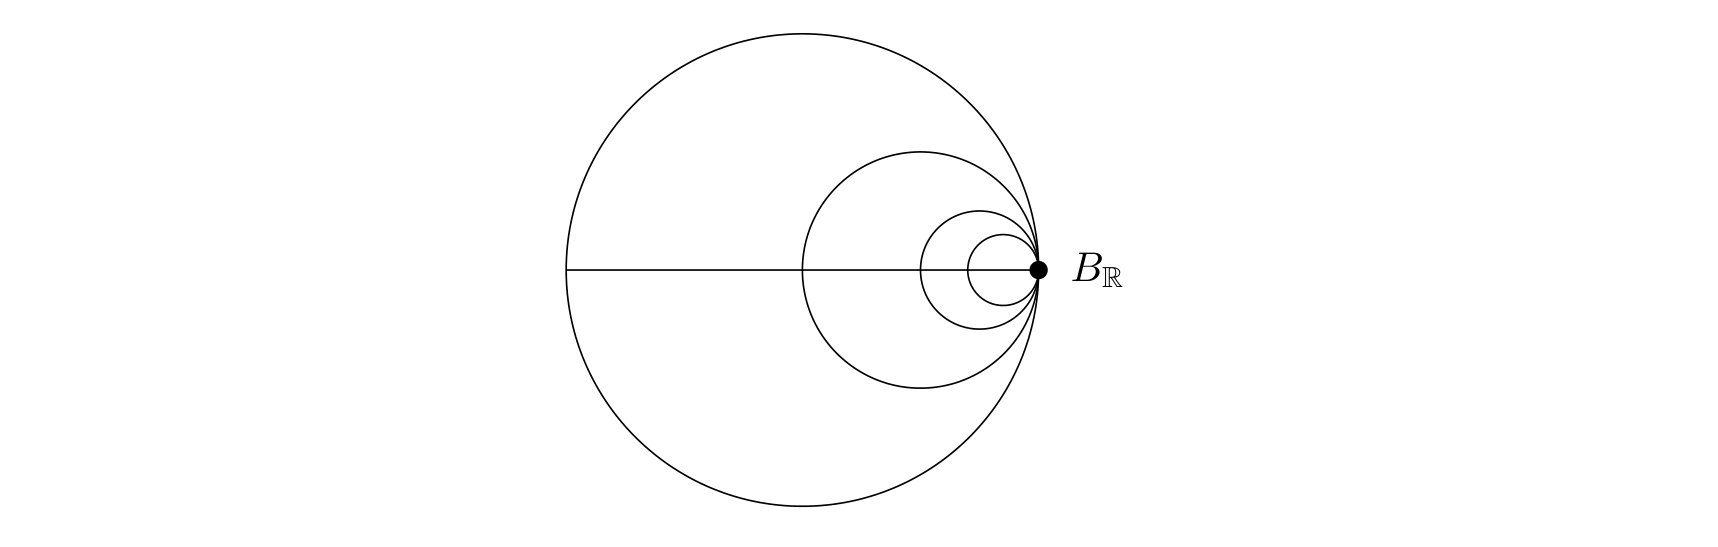
\includegraphics[width=0.42\textwidth]{figure11-3.png}
  \caption{$H=SL_2/SO_2=G_{\R}/K$的 Poincar\'e 圆盘模型。边界上的点对应$B_{\R}$，水平线是一条$T$-轨道，而极限圆（与无穷远点相切的小圆）是$N$-轨道。（原文 p.~198，Figure 11.3）}
  \label{fig:11-3}
\end{figure}

\paragraph{Poincar\'e 圆盘与双曲面模型.}
最熟悉的图景是实版本，即空间$G_{\R}/K$。现在$\R$扮演局部域的角色，因此从复几何的角度看，它与建筑和$\Gr$看起来完全不同。这是双曲空间：
\begin{equation}\tag{11.125}
SL_2(\R)/SO_2\simeq H.
\end{equation}
例如我们可以通过 Poincar\'e 圆盘模型来思考。内部是$G_{\R}/K$，而无穷远点组成$\R\PP^{1}=G_{\R}/B_{\R}$，即$G_{\R}$的旗流形。

现在取一个无穷远点，即一个 Borel $B_{\R}\subset G_{\R}$。对$SL_2$，这是$\R\PP^{1}$中的一个点，即$\R^{2}$中的一条线，而$B_{\R}$是这条线的稳定化子。有一个相应的环面$T$，相应的$T$-轨道是穿过 Poincar\'e 圆盘中心的直线。

现在我们还想画出$N$-轨道。对$SL_2$，
\begin{equation}\tag{11.126}
N=\left\{\begin{pmatrix}1 & b\\ 0 & 1\end{pmatrix}\right\}.
\end{equation}
$N$-作用固定对应于$B_{\R}$的无穷远点，而轨道由图 11.3 中的极限圆（horocycle）给出。

于是我们有$\Gr$的类比——双曲空间$SL_2\R/SO_2$，并且可以映到$SL_2\R/N$，后者称为极限圆空间。然后我们有极限圆对应，它由点$x\in H$连同过它的一条极限圆组成，这个对应空间构成$SL_2(\R)$（模去一个符号）：
\begin{equation}\tag{11.127}
\begin{array}{ccc}
 & SL_2(\R)/(\pm 1) & \\
 \swarrow & & \searrow\\
 SL_2\R/SO_2 & & SL_2\R/N
\end{array}
\end{equation}
极限圆空间实际上可以描述为
\begin{equation}\tag{11.128}
SL_2\R/N\simeq\R^{2}\setminus\{0\}.
\end{equation}

\begin{figure}[htbp]
  \centering
  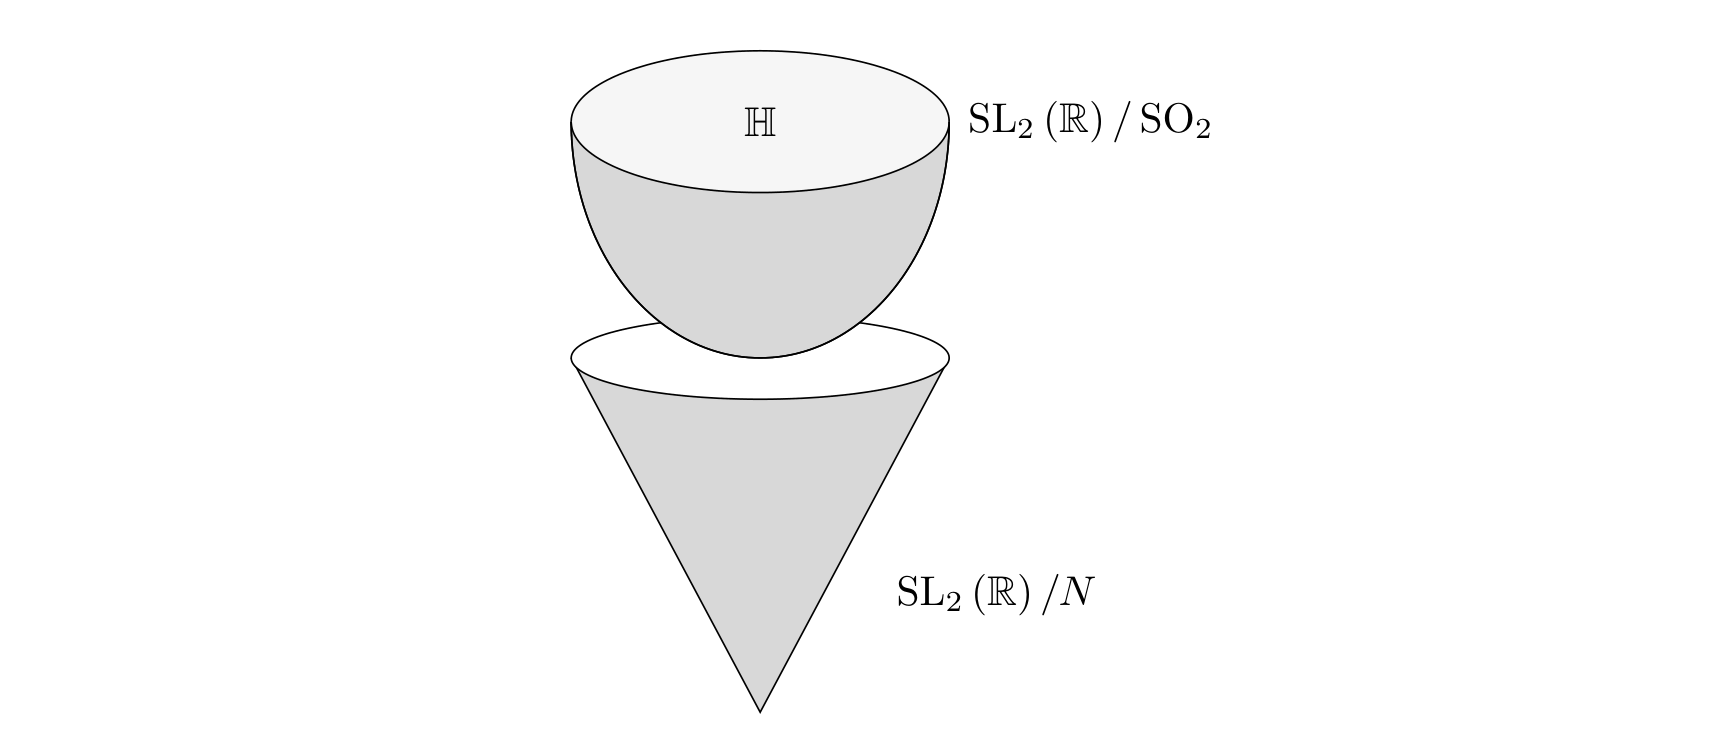
\includegraphics[width=0.42\textwidth]{figure11-4.png}
  \caption{若把$SL_2/SO_2$模型化为双曲面，则可以把极限圆空间$SL_2(\R)/N$看成光锥。（原文 p.~199，Figure 11.4）}
  \label{fig:11-4}
\end{figure}

若把双曲空间模型化为双曲面，这就更容易看出。此时$SL_2\R/N$是$\R^{3}$中的光锥，而$H$作为其中一张叶出现，如图 11.4。在$\infty$附近，$H$看起来像光锥模$\R^{\times}$，即$\R\PP^{1}$。也就是说，我们有一个映射
\begin{equation}\tag{11.129}
\begin{array}{c}
SL_2(\R)/N\simeq\R^{2}\setminus\{0\}\\[2pt]
\downarrow\\[2pt]
\R\PP^{1}=SL_2(\R)/B\\[2pt]
\text{（在 distinguished 点上的纤维为环面 }T\text{）}
\end{array}
\end{equation}
给定$H$上的函数，我们能做的一个自然测量就是沿其中一条极限圆积分。或者我们可以把这看成积分变换。即给定$f\in L^{2}(H)$，我们可以通过 (11.127) 拉回并前推，得到极限圆空间$SL_2(\R)/N$上的函数，即这个光锥上的函数。然后我们可以把它限制到光锥内的任意一条射线上，每条射线对应一个环面$T$。即我们从$H$上的函数出发，拉回、前推、再限制，得到$T$上的函数。现在我们可以用 Fourier 理论分解这个函数。这一程序称为 Harish-Chandra 变换。

为完成与$\Gr_G$的类比，极限圆就是半无限轨道$S_\lambda\subset\Gr$的类比。$\sph$的纤维函子由限制到轨道再前推给出。这里对应的是限制到极限圆再平均（积分）。

还要注意，在图 11.3 中，穿过无穷远不动点的极限圆恰好由$T$-轨道标号。这就是前面“$N(K)$-轨道集合与$\Gr_T$一一对应”这一陈述的类比。

\paragraph{建筑.}
回忆$PSL_2$建筑的顶点是$K^{2}$中的$\cO$-格模去伸缩（即模去位似）。所得的图是图 9.1 和图 9.2 所示的 3-正则树。在无穷远处，这棵树看起来像$\PP^{1}(K)$。极限圆图景的类比如下。

选择一个无穷远点。形式上这意味着树的一个端（end）。这是一个道路的等价类。两条道路若最终在通向无穷远的路上某点重合，即它们只相差有限多个顶点/边，就称等价。

一旦选定了树的一个端，我们就可以考虑距离给定端固定距离的所有顶点的集合。我们说两个顶点$V_1$和$V_2$到该端的距离相同，若存在（在该端的等价类中的）道路$P_1$和$P_2$满足：由于$P_1$和$P_2$在该端的等价类中，它们最终重合，即只相差有限多个顶点；我们要求$P_1$中而不在$P_2$中的边数等于$P_2$中而不在$P_1$中的边数。固定距离的顶点构成一条极限圆。当我们如图 11.5 画出树的公寓（apartment）时，这一点更清楚。这个拉直后的公寓图景是上半空间模型的类比。特定的无穷远点是$i\infty\in H$，而极限圆（$N_{\R}$-轨道）是$H$中的水平线。

\begin{figure}[htbp]
  \centering
  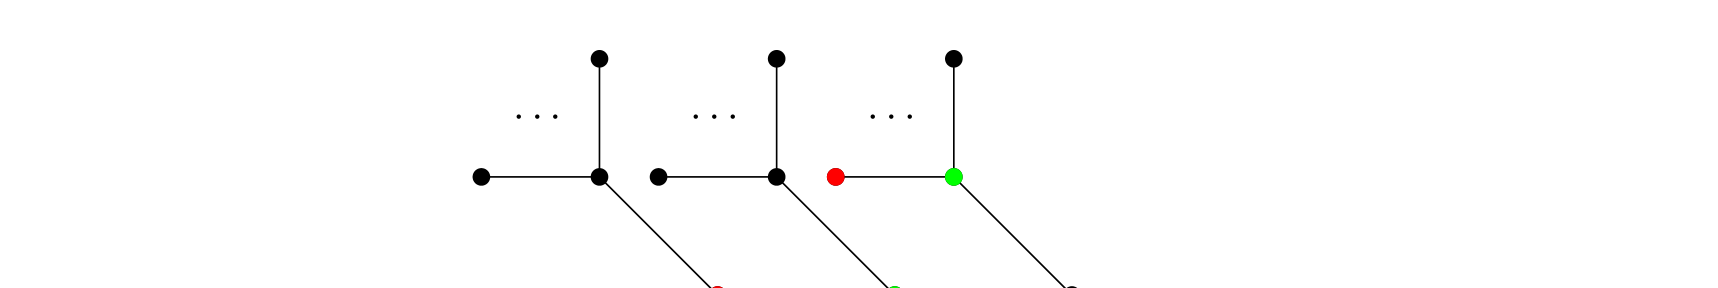
\includegraphics[width=0.5\textwidth]{figure11-5.png}
  \caption{图 9.2 中 3-正则树的公寓。绿色顶点彼此到该端的距离相同，红色顶点到该端的距离也相同。（原文 p.~200，Figure 11.5）}
  \label{fig:11-5}
\end{figure}

% [Tutor Note: (11.125) 中的$H$是双曲平面；$G_{\R}/K$与$\Gr_G$的类比并非同构，而是“非紧对称空间 vs. 仿射 Grassmann 流形”的层次类比。这里$N_{\R}$-轨道（极限圆）对应$N(K)$-轨道（半无限轨道$S_\lambda$），而$T$-轨道对应不动点格$\Gr_T\simeq\Lambda$；Mirkovi\'c–Vilonen 的纤维函子正是“沿极限圆积分”的代数版本。]

\section{谱分解}\label{sec:11-7}

\begin{sectionkey}
本节把$\sph\simeq\Rep(G^{\vee})$的作用推广到曲线上的每一点，得到$\otimes'_{x\in C}\Rep(G^{\vee})$在$\Shv(\Bun_G(C))$上的作用，并猜想它分解到 \term{Langlands 参数空间}{space of Langlands parameters} $\Loc_{G^{\vee}}(C)$上；谱纤维的对象即 Hecke 特征层，对应调和分析中的特殊函数。
\end{sectionkey}

\begin{flushright}\small 第 29 讲；2021 年 5 月 20 日\end{flushright}

\subsection{Langlands 对偶群}\label{sec:11-7-1}

回忆我们把几何 Satake 对应看作描述理论$A_G$的线算子$\otimes$-范畴：
\begin{equation}\tag{11.130}
\sph:=A_G(S^{2})=\Shv(LG_+\backslash LG/LG_+).
\end{equation}
它以 Hecke 修正作用在$\Shv(\Bun_G(C))$上。然后几何 Satake 的结果是
\begin{equation}\tag{11.131}
(\sph,*)\simeq\Rep(G^{\vee}),
\end{equation}
其中$G^{\vee}$是 Langlands 对偶群。这是$k$上的约化代数群（$k$是我们的层的系数域）。

这个群$G^{\vee}$有一些粗特征，例如
\begin{equation}\tag{11.132}
\pi_1(G)\simeq Z(G^{\vee})^{\vee}.
\end{equation}
所以若$G$单连通，则$G^{\vee}$是伴随型（无中心）。对极大环面$T\subset G$，对偶环面$T^{\vee}$是$G^{\vee}$的极大环面。事实上，$G^{\vee}$的构造自带对偶环面，所以$G^{\vee}$真正是一个分裂约化群。

\begin{srcrem}{82}
$G^{\vee}$实际上自带一个 pinning。所以它带有环面$T^{\vee}\subset G^{\vee}$，但也带有一个典范余特征
\begin{equation}\tag{11.133}
G_m\subset T^{\vee}\subset G^{\vee},
\end{equation}
我们将称之为$2\rho^{\vee}$。这个包含对应于纤维函子
\begin{equation}\tag{11.134}
\Vect^{\Z\text{-gr}}\leftarrow\Vect^{\Lambda\text{-gr}}\leftarrow\Rep G^{\vee}.
\end{equation}
要点是：纤维函子$\sph\to\Vect$分解为上同调到分次向量空间的函子与$\operatorname{Forget}$：
\begin{equation}\tag{11.135}
\Vect\xleftarrow{\ \operatorname{Forget}\ }\Vect^{\Z\text{-gr}}\xleftarrow{\ H^{*}\ }\sph.
\end{equation}
\end{srcrem}
特别地，这个典范的$G_m\subset T^{\vee}$给出表示的典范分次，这为我们挑出一个 Borel（所有正的东西）。

\begin{srcex}{78}
从环面$T$出发，Langlands 对偶就是对偶环面$T^{\vee}$。$GL_n$的 Langlands 对偶是它自己：
\begin{equation}\tag{11.136}
GL_n^{\vee}=GL_n.
\end{equation}
Langlands 对偶交换伴随型和单连通群，例如
\begin{equation}\tag{11.137}
PGL_n^{\vee}=SL_n.
\end{equation}
$D_n$型自对偶：
\begin{equation}\tag{11.138}
SO_{2n}^{\vee}=SO_{2n}.
\end{equation}
另一方面，$B_n$型与$C_n$型互换：
\begin{equation}\tag{11.139}
SO_{2n+1}^{\vee}=Sp_{2n}.
\end{equation}
\end{srcex}
这是要记住的：群$SO_{2n+1}$与$Sp_{2n}$看起来并无关系（例如它们的几何非常不同），但它们的组合数据是对偶的。这就是为什么涉及 Langlands 对偶的东西往往非常深刻：所涉及的群往往（以显然的方式）互不相关。

\subsection{本征对象}\label{sec:11-7-2}

回忆我们引入这个范畴来作用于事物。设$C$是黎曼面/代数曲线。则对$x\in C$我们得到一个作用：$\sph\circlearrowright\Shv(\Bun_G(C))$。具体地，$V\in\sph$定义$\operatorname{Hecke}_x$上的层，它通过对应
\begin{equation}\tag{11.140}
\begin{array}{ccc}
 & \operatorname{Hecke}_x & \\
 \swarrow & & \searrow\\
 \Bun_G & & \Bun_G
\end{array}
\end{equation}
给出从$\Bun_G$上的层到自身的积分变换。回忆我们在例 70 和 71 中对$G=GL_n$见过这一点。所以我们有一个交换$\otimes$-范畴$\sph\simeq\Rep(G^{*})$在范畴$\Shv(\Bun_G)$上的作用，并想作谱分解。于是我们要识别\term{本征对象}{eigenobject}，即我们只是试图同时对角化一堆算子。

本征对象是一个对象$F\in\Shv(\Bun_G)$连同一个同构
\begin{equation}\tag{11.141}
V*F\xrightarrow{\ \sim\ }E_x(V)\otimes F
\end{equation}
对$V\in\Rep(G^{\vee})\simeq\sph$。即$E_x(-)$是“本征值”。这是一个函子
\begin{equation}\tag{11.142}
E_x\colon\Rep(G^{\vee})\xrightarrow{\ \otimes\ }\Vect.
\end{equation}
用我们的 Tannakian 故事，我们可以容易地写下本征值。要点是$\Rep(G^{\vee})=\Shv(\mathrm{pt}/G^{\vee})$而$\Vect=\Shv(\mathrm{pt})$，所以这样的函子等价于一个映射$\mathrm{pt}\to\mathrm{pt}/G^{\vee}$。但这样的映射在相差同构的意义下只有一个。等价地，这样的映射由一个$G^{\vee}$-torsor $E_x$给出。然后给定$V\in\Rep(G^{\vee})$，我们可以把它送到伴随向量丛：$(V)_{E_x}\in\Vect$。

现在我们可以做两件事：变化点，或去范畴化（取某些迹）。首先我们变化点。

% [Tutor Note: (11.142) 中“$\otimes$标记的箭头”表示这是张量函子（$\otimes$-functor）；$E_x$之所以由$G^{\vee}$-torsor 给出，是因为 Tannakian 对偶把$\Shv(\mathrm{pt})$上的张量函子等同于$\mathrm{pt}/G^{\vee}$的一个点（即$G^{\vee}$-torsor）。原文把$G^{\vee}$的法向分次（由$2\rho^{\vee}$给出）单独列出，是为了让“本征值”与表示的分次相容。]

\subsection{变化点}\label{sec:11-7-3}

现在我们变化点$x\in C$。于是不再由单个$\Rep(G^{\vee})$拷贝作用，而是将由$C$的某个点集上每个点处的一个这样的范畴作用。

更形式地，我们有一个受限张量积\footnote{这与之前受限积类似定义：除有限多个“条目”外均为平凡。}的作用：
\begin{equation}\tag{11.143}
\bigotimes'_{x\in C}\Rep(G^{\vee})\circlearrowright\Shv(\Bun_G(C)).
\end{equation}
即我们在一大堆点处作修正，而不只是在一个点。

我们一直有一个基本假设：周围有一个拓扑场论。即我们受到$A_G(C)=\Shv(\Bun_G(C))$这一想法的驱动，而上面的作用应由线算子范畴给出。它来自 TFT 这一事实意味着线算子的作用局部地、常数地依赖于$x\in C$。于是这个作用通过$R_C\Rep(G^{\vee})$的作用分解：
\begin{equation}\tag{11.144}
\begin{array}{ccc}
\bigotimes'_{x\in C}\Rep(G^{\vee}) & \longrightarrow & \Shv(\Bun_G(C))\\
 & \searrow & \nearrow\\
 & & R_C\Rep(G^{\vee})
\end{array}
\end{equation}
事实上我们说过：
\begin{align}
\Spec\int_C\Rep(G^{\vee})&=\operatorname{Map}_{lc}(C,\mathrm{pt}/G^{\vee})\tag{11.145}\\
&=\Loc_{G^{\vee}}(C).\tag{11.146}
\end{align}

\begin{srcrem}{83}
$\Loc_{G^{\vee}}(C)$在拓扑/Betti 情形下极其简单。具体地，它是
\begin{align}
\Loc_{G^{\vee}}(C)&=\{\pi_1(C)\to G^{\vee}\}/G^{\vee}\tag{11.147}\\
&=\Bigl\{A_1,\dots,A_g,B_1,\dots,B_g\in G^{\vee}\ \Big|\ \prod_i A_iB_iA_i^{-1}B_i^{-1}=1\Bigr\}/G^{\vee},\tag{11.148}
\end{align}
因为黎曼面的基本群有$A$、$B$圈的这种简单呈现。
\end{srcrem}

这一认识的结果是，如果我们相信它来自一个场论：
\begin{equation}\tag{11.149}
A_G(C)=\Shv(\Bun_G(C)),
\end{equation}
那么$\bigotimes'\Rep G^{\vee}$在其上的作用分解为
\begin{equation}\tag{11.150}
\begin{array}{ccc}
\bigotimes'_{x\in C}\Rep(G^{\vee}) & \longrightarrow & \Shv(\Bun_G(C))\\
 & \searrow & \nearrow\\
 & & \QC(\Loc_{G^{\vee}}(C))
\end{array}
\end{equation}
事实上，沿着这些思路有一些（非常深刻且困难的）定理，适用于各种版本的$\Shv$。

\begin{srcthm}{10（Gaitsgory 消没定理）}
这在 de Rham 情形成立。即朴素的 Hecke 作用
$\QC(\Loc^{dR}_{G^{\vee}})\circlearrowright D(\Bun_G(C))$通过相应的整体对象分解。
\end{srcthm}

\begin{srcthm}{11（Nadler–Yun）}
这在 Betti 情形成立，其中我们的层具有幂零奇异支撑：$\Shv_N(\Bun_G(C))$。
\end{srcthm}

\begin{srcrem}{84}
$\Shv_N(\Bun_G(C))$是我们从$\Bun_T$、$\Bun_L$（$L$为 Levi 子群）上的局部常值层出发并诱导得到的范畴。
\end{srcrem}

\begin{srcthm}{12（Arinkin–Gaitsgory–Kazhdan–Raskin–Rozenblyum–Varshavsky）}
这在受限情形（在$\F_q$上）成立。\footnote{这算是 de Rham 世界与 Betti 世界的交叠，即某种“核心”的几何 Langlands。}
\end{srcthm}

这告诉我们$\Shv(\Bun_G(C))$在$\Loc_{G^{\vee}}$（Langlands 参数空间）上谱分解。即$A_G(C)$是$\Loc_{G^{\vee}}$上的范畴层。这是 Langlands 对应的要点之一。

我们能问的最具体的东西是某点$E\in\Loc_{G^{\vee}}$处的纤维。这将是$E$-Hecke \term{特征层}{eigensheaf}的集合。这是一个层$F\in\Shv(\Bun_G)$连同同构
\begin{equation}\tag{11.151}
V_x*F\xrightarrow{\ \sim\ }(V_x)_{E_x}\otimes F
\end{equation}
对所有$x\in C$和$V\in\Rep(G^{\vee})$成立。即$F$是曲线上每一点处 Hecke 算子的本征对象，本征值是$E\in\Loc_{G^{\vee}}$，即我们在每点有本征值（$G^{\vee}$-torsors），并把它们拼成局部常值层$E$。

这些是调和分析中特殊函数概念在范畴层面的类比。特殊函数往往满足非常好的微分方程组。特别地，交换微分算子族的本征函数就是特殊函数，例如指数函数$e^{\lambda x}$。所以 Hecke 特征层是$e^{\lambda x}$的类比，其中本征值$\lambda$现在被曲线$C$上的$G^{\vee}$-局部系统$E$取代。

我们在交换情形谈过 Hecke 特征层，那时可以用例如 Abel–Jacobi 映射或 Fourier–Mukai 变换来构造它们。但在非交换情形没有容易的构造方法。对任何特定的局部系统，都不清楚是否存在。但这仍把我们引向朴素的几何 Langlands 猜想。

% [Tutor Note: 11.7.2 开头原文把右端误写作$\Rep(G^{*})$（星号），其后一律为$G^{\vee}$；译文保留该处笔误形式以对应原文，读者应读作$G^{\vee}$。(11.145) 的$\operatorname{Map}_{lc}$指局部常值映射，其叠结构使$\Spec$只能取导出意义；原文在 Betti 情形下不加导出修饰，读者需自行补上。]

\section{朴素的几何 Langlands 猜想}\label{sec:11-8}

\begin{sectionkey}
本节陈述朴素猜想$A_G(C)\simeq\QC(\Loc_{G^{\vee}})$，指出它因$\Loc_{G^{\vee}}$的奇点而失败，并说明修正方向：限制到不可约局部系统（对应$B$-侧的尖点层）或改用导出/幂零支撑版本；最后把几何 Satake 解释为$A_G$与 4 维 B-模型之间的线算子匹配。
\end{sectionkey}

朴素的几何 Langlands 猜想大致是说：存在足够多的 Hecke 特征层，且它们张成整个范畴。也就是说
\begin{equation}\tag{11.152}
A_G(C)\simeq\QC(\Loc_{G^{\vee}}),
\end{equation}
其中摩天楼层$\cO_E\in\QC(\Loc_{G^{\vee}})$对应于一个 Hecke 特征层$A_E\in A_G(C)$，后者在相差一个标量的意义下唯一。

\begin{srcrem}{85}
这类似于低一层的图景：指数函数张成$L^{2}$意味着我们有 Fourier 变换。
\end{srcrem}

于是对每个$E\in\Loc_{G^{\vee}}$我们得到$A_E\in A_G(C)$，在相差标量意义下唯一。等价地说，这是在说
\begin{equation}\tag{11.153}
\QC(\Loc_{G^{\vee}})\circlearrowright\Shv(\Bun_G)
\end{equation}
是自由秩$1$模。换言之，这个模由本征向量张成。更具体地，我们可以选一个合适的循环向量让它作用，例如 Whittaker 层，于是这是说诱导出的态射是等价：
\begin{equation}\tag{11.154}
\QC(\Loc_{G^{\vee}})\xrightarrow{\ \sim\ }\Shv(\Bun_G).
\end{equation}
这是 Fourier 理论中单位元处摩天楼层的类比。

这个猜想按原样并不成立，这一点早已为人所知。基本问题在于叠$\Loc_{G^{\vee}}$是奇异的，而$\QC(\Loc_{G^{\vee}})$检测不到这些奇点。所以我们可以苦思并修正它，或者限制到$\Loc_{G^{\vee}}$内一个由不可约局部系统组成的开稠密轨迹。对$G=GL_n$，这恰指不可约的带平坦联络向量丛（即没有在平行移动下封闭的子丛）。一般而言，一个局部系统不可约，若它没有平坦的到抛物子群的约化。于是我们有由不可约局部系统组成的开稠密轨迹$\Loc^{irr}_{G^{\vee}}$。结果这是一个光滑叠，几乎是一个簇。若$E$不可约，则
\begin{equation}\tag{11.155}
\Aut(E)=Z(G^{\vee}).
\end{equation}
例如若$G$单连通，则$G^{\vee}$伴随，故这些自同构是平凡的。所以此时$\Loc^{irr}_{G^{\vee}}$构成一个光滑簇。

无论如何，猜想预期在这个轨迹上成立。$G=SL_2$的情形归功于 Drinfeld，$G=GL_n$的情形归功于 Gaitsgory。（原文此处附引用标记。）

限制到不可约局部系统在另一侧对应什么？不可约局部系统意味着没有到抛物子群$P^{\vee}\subset G^{\vee}$的约化，这等价于不在任何映射的像中：$\Loc_{P^{\vee}}\to\Loc_{G^{\vee}}$。特别地，它与这些抛物诱导/Eisenstein 级数对应没有交互：
\begin{equation}\tag{11.156}
\begin{array}{ccc}
 & \Loc_{P^{\vee}} & \\
 \swarrow & & \searrow\\
 \Loc_{G^{\vee}} & & \Loc_{G^{\vee}}
\end{array}
\end{equation}
即它与 Eisenstein 级数没有交互。

在 Langlands 对应的另一侧，这意味着我们在找$F\in\Shv(\Bun_G)$使得抛物限制
\begin{equation}\tag{11.157}
\begin{array}{ccc}
 & \Bun_P & \\
 \swarrow & & \searrow\\
 \Bun_G & & \Bun_L
\end{array}
\end{equation}
为零。这就是\term{尖点}{cuspidal}的定义。

\begin{srcex}{79}
尖形式（cusp form）是在$\infty$处为$0$的模形式。结果这等价于常数项为$0$。回忆常数项由沿一条水平线/极限圆积分给出，而这个操作恰好是从$PSL_2\to T$的抛物限制。
\end{srcex}
所以$B$-侧尖点的层应当与$A$-侧不可约轨迹上的层相匹配。

\paragraph{为什么它不能成立.}
朴素的几何 Langlands 猜想失败，原因如下。对应于
\begin{equation}\tag{11.158}
E=\mathrm{triv}\in\Loc_{G^{\vee}}(C)
\end{equation}
的$\Bun_G$上的“那个”自守层是什么？平凡局部系统是最糟糕的点。它是最奇异/最像栈（自同构最多）的点。看出这令人困惑的一种方式是：$\mathrm{triv}$来自$\mathrm{triv}_{T^{\vee}}$。但它也来自任何 Levi $L$的$\mathrm{triv}_{L^{\vee}\subset G^{\vee}}$。而 Eisenstein 级数理论给我们一个公式：
\begin{equation}\tag{11.159}
A_{\mathrm{triv},L^{\vee}}\in\Shv(\Bun_G),
\end{equation}
通过做某种版本的抛物诱导，而它们全都不同。所以我们有一堆层，它们都想以平凡局部系统作为本征值。

另一个密切相关的事情是尝试$\Bun_G$上最显然的层，即常值层$k$。它是 Hecke 特征层吗？当我们在$x$处作用 Hecke 算子$V_x$于$k$上时，得到$V_x*k$，它是$k$的拉回限制到某个$G(\cO)$-轨道（或更一般地，把它与$\Gr$上某个层作张量）后的前推。所以结果是层$H_V\in\Shv(\Gr)$的上同调与$k$张量。于是对任意点$x\in C$我们得到同样的东西：$k$与这个上同调张量，它可能生活在非零次数。这称为 Arthur 特征层。这些正是我们缺失的那类东西。

\subsection{朴素的电磁/Montonen–Olive $S$-对偶}\label{sec:11-8-1}

一旦我们对朴素几何 Langlands 猜想感觉良好，就可以放开手脚，作朴素的猜测：整个理论$A_G$等价于$B^{\mathrm{naive}}_{G^{\vee}}$，即$\mathrm{pt}/G^{\vee}$上的 4 维 B-模型（回忆第 10.7 节）。回忆它给出：
\begin{align}
B^{\mathrm{naive}}_{G^{\vee}}(M^{3})&=\cO(\Loc_{G^{\vee}}(M))\tag{11.160}\\
B^{\mathrm{naive}}_{G^{\vee}}(\Sigma^{2})&=\QC(\Loc_{G^{\vee}}(\Sigma))\tag{11.161}\\
B^{\mathrm{naive}}_{G^{\vee}}(N^{1})&=\Shv\mathrm{Cat}(\Loc_{G^{\vee}}(N)).\tag{11.162}
\end{align}
与其说这是猜想的“朴素”版本，不如说这是第一近似。回忆我们是用线算子范畴构造$G^{\vee}$（从而构造$B^{\mathrm{naive}}_{G^{\vee}}$）的。我们本可以从局部算子出发得到第零近似，但在这个（非导出的）情形下那会是平凡的。这个理论可能不包含匹配理论$A_G$所需的全部信息，但它们几乎相同。

若$A_G$与$B_{G^{\vee}}$作为场论等价，这当然意味着线算子及其作用必须一致。在$A$-侧我们有$A_G(S^{2})=\sph$，而在$B$-侧我们有
\begin{equation}\tag{11.163}
B_{G^{\vee}}(S^{2})=\QC\bigl(\Loc_{G^{\vee}}(S^{2})\bigr).
\end{equation}
由于$S^{2}$单连通，$\Loc_{G^{\vee}}(S^{2})\simeq\mathrm{pt}/G^{\vee}$，所以至多差一些导出增强，我们得到
\begin{equation}\tag{11.164}
\QC\bigl(\Loc_{G^{\vee}}(S^{2})\bigr)=\QC(\mathrm{pt}/G^{\vee}).
\end{equation}
即便我们（导出地）正确地说这件事，仍然有
\begin{equation}\tag{11.165}
\Rep(G^{\vee})\subset\QC\bigl(\Loc_{G^{\vee}}(S^{2})\bigr).
\end{equation}
这些是 Wilson 线算子。我们可以如下显式地看出这个作用。设$C$是黎曼面，$x\in C$，$V\in\Rep(G^{\vee})$。则我们如下得到$\Loc_{G^{\vee}}(C)$上的向量丛。对任何局部系统，我们可以考虑$V$的伴随向量丛，并取它在$x$处的纤维：
\begin{equation}\tag{11.166}
E\mapsto(V)_{E_x}.
\end{equation}
也就是说，有一个由拉回给出的函子
\begin{equation}\tag{11.167}
\Rep(G^{\vee})\xrightarrow{\ i_x^{*}\ }\QC(\Loc_{G^{\vee}}),
\end{equation}
其中
\begin{equation}\tag{11.168}
i_x\colon\Loc_{G^{\vee}}\to\mathrm{pt}/G^{\vee}
\end{equation}
取$x$处的纤维。换言之，给定$x\in C$和$V\in\Rep(G^{\vee})$有一个算子
\begin{equation}\tag{11.169}
V*(-)\colon\QC(\Loc_{G^{\vee}})\to\QC(\Loc_{G^{\vee}}).
\end{equation}
这些就是 Wilson 线算子。

于是朴素等价$A_G$与$B^{\mathrm{naive}}_{G^{\vee}}$蕴含线算子在两侧必须匹配：
\begin{equation}\tag{11.170}
A_G(S^{2})\simeq B_{G^{\vee}}(S^{2}).
\end{equation}
这个陈述就是几何 Satake。在谱/$B$-侧，线算子就是这些非常简单的 Wilson 线；而在自守/$A$-侧我们有的是更复杂的 't Hooft 线。然后几何 Satake 告诉我们它们相同。

接着朴素几何 Langlands 猜想说我们有一个范畴等价，并且对每个点$x\in C$有相容的作用：
\begin{equation}\tag{11.171}
\begin{array}{ccc}
\Shv(\Bun_G) & \xrightarrow{\ \simeq\ } & \QC(\Loc_{G^{\vee}})\\
\uparrow & & \uparrow\\
\sph & \xrightarrow{\ \simeq\ } & \Rep(G^{\vee})
\end{array}
\end{equation}

\begin{flushright}\small 第 30 讲；2021 年 5 月 27 日\end{flushright}

% [Tutor Note: (11.152) 按原样不成立，正确的修正通常是把$\QC$换成$\IndCoh$（Arinkin–Gaitsgory 的“修正几何 Langlands 猜想”），因为$\Loc_{G^{\vee}}$奇异时$\QC$丢失了导出信息；这也是 (11.165) 只能是包含而非等号的原因。(11.159) 中的$A_{\mathrm{triv},L^{\vee}}$依赖 Levi $L$，不同$L$给出不同的 Eisenstein 层，但都以平凡局部系统为本征值——这正是“本征值不能唯一确定本征对象”的表现。]


\chapter{范畴化}\label{ch:12}

\begin{keytakeaways}
本章讨论范畴化（categorification）及其几何来源。范畴化是把数替换为向量空间（或范畴）、把向量空间替换为范畴的病态逆过程；其严格形式由 TFT 给出：与$S^{1}$作积对应于取维数，\term{映射环面}{mapping torus}对应于取迹。于是“维数”“迹”在\term{配边}{bordism}范畴$\Bord$、对应范畴$\mathrm{Corr}$与线性目标范畴$\cC$中分别呈现为$(-)\times S^{1}$、不动点$\mathcal{L}(-)$与$\HH_{*}$/$\chi$，并由对称幺半函子保证三者相容。几何上，迹就是不动点，这给出 Lefschetz 不动点公式与 Grothendieck–Lefschetz 迹公式，进而引出函数-层对应、Lusztig 特征层与 Kazhdan–Lusztig 理论。最后，几何 Satake 对应被解释为球 Hecke 范畴的范畴化，它比经典 Satake 同构更强，因为 Tannakian 重构能真正构造出 Langlands 对偶群。
\end{keytakeaways}

\section{基础}\label{sec:12-1}

\begin{sectionkey}
本节给出范畴化的非形式定义：一个数若能实现为某向量空间的维数（或分次向量空间的 Euler 特征、某算子的迹），就称该向量空间范畴化了这个数；Grothendieck 群$K_0$是把范畴映回向量空间的标准去范畴化不变量。
\end{sectionkey}

众所周知，\term{范畴化}{categorification}并没有严格定义。它毋宁是所谓的\term{去范畴化}{decategorification}的一个病态逆过程。基本想法是：给定一个数，人们希望它作为某个向量空间的维数出现。当然，只有自然数能这样出现；但给定一个自然数，人们希望它来自一个向量空间，而后者携带的信息严格多于该数本身。此时称这个数是该向量空间的去范畴化。

\begin{srcex}{80}
拓扑空间的 Betti 数是同调群的维数。即对拓扑空间$X$，$H_i(X)$的去范畴化是$b_i(X)$。
\end{srcex}

若我们有一个整数（可能为负），我们仍希望它来自某个向量空间，只是此时要问它是否为某个分次向量空间的 Euler 特征。

于是范畴化就是试图用一个自然的向量空间去替换一个数的病态过程，使得它成为去范畴化的逆。也就是说，一个向量空间范畴化一个数，若该数是这个向量空间的去范畴化/维数/Euler 特征。

这可以如下推广。除了向量空间$V$，人们可能还有别的线性代数数据，例如算子$O\in\End(V)$。此时我们可能期待给定的数作为$\operatorname{Tr}(O)$出现。要点是：算子的迹不总是整数。

\begin{srcex}{81}
若$O=\mathrm{id}$，则$\operatorname{Tr}(\mathrm{id})=\dim$，于是这退化为上面以$\dim$或$\chi$为去范畴化的概念。
\end{srcex}

\begin{srcex}{82}
设$G\circlearrowright V$是群的表示。$V$的特征是一个定义在$G$上的函数$\chi$，它把$g\in G$送到$g$的迹，这里把$g$看成$V$上的算子。于是我们不止有一个数，而是有一族数，以$g\in G$为指标，作为$g\colon V\to V$的迹出现。
\end{srcex}

这族数$\{\operatorname{Tr}(g)\}_{g\in G}$定义了元素$\chi_V\in\C^{G}_{G}$，即它定义了向量空间的一个元素，然后我们把它升级为真正的表示$V\in\Rep(G)$。

所以在这个例子里，我们从向量空间的一个元素出发，然后把它升级为范畴的一个对象。因此我们可以把这个过程重新表述为：从向量空间出发，把它升级为范畴。这就是这个过程称为范畴化的原因。

这个向量空间显式地由范畴的 Grothendieck 群给出，例如：
\begin{equation}\tag{12.1}
\C^{G}_{G}=K_0(\Rep(G)).
\end{equation}
所以我们可能从一个数出发，它由某个向量空间的维数或 Euler 特征给出；也可能从一个向量空间出发，它由某个范畴的不变量（如$K_0$）给出。

\begin{srcrem}{86}
正如一个数的正性是它是某种更深结构的影子（即它是$\dim(V)$，或它来自组合计数）的标志，向量空间的一组自然基也可以看成某种更深结构（即它是某个范畴的$K_0$）的影子。例如，若我们的范畴中有单对象或投射对象，它们可能下降为 Grothendieck 群的自然基。
\end{srcrem}

\begin{srcex}{83}
函数空间是向量空间的自然来源。它们往往来自层的范畴。于是几何给我们自然的范畴与自然的向量空间，再由去范畴化程序联系起来。
\end{srcex}

% [Tutor Note: 这里的$\C^G_G$是$G$上的类函数空间（即$G$在$\C[G]$上的不变量，或等变层$\Shv(G/G)$的截面），并非“$G$的平方”；$K_0(\Rep(G))$与类函数空间在系数域上同构，正是特征标理论的起点。若把$G$换为有限群，$K_0(\Rep(G))$就是表示环。]

\section{（去）范畴化与 TFT}\label{sec:12-2}

\begin{sectionkey}
本节说明 TFT 如何给出范畴化的严格框架：与$S^{1}$作积对应取维数，映射环面对应取迹，而对偶性与 Mark of Zorro 关系是这一切的代数基础。
\end{sectionkey}

设$Z$是一个 TFT。有一个自然的操作：在把$Z$作用到配边上之前，先把它与$S^{1}$作积，即我们考虑$Z\bigl((-)\times S^{1}\bigr)$。一般的口号是
\begin{equation}\tag{12.2}
Z\bigl((-)\times S^{1}\bigr)=\dim Z(-).
\end{equation}
设$Z$是一维 TFT。回忆第 10.1 节：
\begin{equation}\tag{12.3}
\begin{array}{rcl}
Z(\varnothing)&=&\C\\
Z(\bullet^+)&=&V\\
Z(\bullet^-)&=&V^{\vee},
\end{array}
\end{equation}
其中$V$是向量空间，$V^{\vee}$是其对偶。于是配边
\begin{equation}\tag{12.4}
\overset{+\ \ -}{\smile}
\end{equation}
定义了线性映射
\begin{equation}\tag{12.5}
\C\to V\otimes V^{\vee}.
\end{equation}
类似地，配边
\begin{equation}\tag{12.6}
\overset{+\ \ -}{\frown}
\end{equation}
定义了线性映射
\begin{equation}\tag{12.7}
V\otimes V^{\vee}\to\C.
\end{equation}
那么由$S^{1}$定义的配边$\varnothing\to\varnothing$是这两个配边的复合：
\begin{equation}\tag{12.8}
\bigcirc=\overset{+\ \ -}{\frown}\circ\overset{+\ \ -}{\smile},
\end{equation}
因此被赋予这两个映射的复合：
\begin{equation}\tag{12.9}
\begin{array}{ccc}
 & V\otimes V^{\vee} & \\
 \mathrm{coev}\nearrow & & \searrow\mathrm{ev}\\
 \C & \xrightarrow{\ \dim(V)\ } & \C
\end{array}
\end{equation}
即
\begin{equation}\tag{12.10}
Z(S^{1})=\dim(V).
\end{equation}
当$Z$取值于$\Vect$，即$V\in\Vect$时，这是一个定理；但若$Z$是更高维的、取值于更一般的目标，则这将作为维数的定义。这是什么意思？设$Z$是$n$维 TFT。对维数$\le n$的配边$M$，我们有
\begin{equation}\tag{12.11}
Z(M)\in\cC
\end{equation}
其中$\cC$是某个对称幺半（高阶）范畴。现在我们有
\begin{equation}\tag{12.12}
Z\bigl(M\times S^{1}\bigr)\in\End(1_{\cC}).
\end{equation}
我们可以把上面的图与$M$作积，得到一个态射
\begin{equation}\tag{12.13}
Z\Bigl(M\times\overset{+\ \ -}{\smile}\Bigr)\colon Z(M)\otimes Z(\overline{M})\to 1_{\cC},
\end{equation}
以及一个态射
\begin{equation}\tag{12.14}
Z\Bigl(M\times\overset{+\ \ -}{\frown}\Bigr)\colon 1_{\cC}\to Z(M)\otimes Z(\overline{M}).
\end{equation}
于是我们可以把$Z(M\times S^{1})$的值计算为复合
\begin{equation}\tag{12.15}
1_{\cC}\to Z(M)\otimes Z(\overline{M})\to 1_{\cC},
\end{equation}
即
\begin{equation}\tag{12.16}
Z(M\times S^{1})=:\dim(Z(M))\colon 1_{\cC}\to 1_{\cC}.
\end{equation}
更形式地，设$V\in\cC$是对称幺半范畴的对象。则$V$可对偶，若存在$V^{\vee}\in\cC$以及态射
\begin{equation}\tag{12.17}
1\to V\otimes V^{\vee},\qquad V^{\vee}\otimes V\to 1
\end{equation}
使得 Mark of Zorro 条件满足。也就是说，在图景中我们有
% 校订注：原裁件只保留左半，「$=$」与右半直线被切掉（原注亦已说明此点）。
% 2026-11-19 由原 PDF p.209 以 400 dpi 重裁整幅，左右两半与「$=$」齐全。
\diageq{12.18}{0.30\textwidth}{p209_d4.png}
% [Tutor Note: (12.18) 左右两半以 “$=$” 相连：左半是“佐罗”曲线
% （$V$ 经 $V^{\vee}$ 绕回 $V$ 的 zig-zag，即 $\mathrm{coev}$ 与 $\mathrm{ev}$ 的复合），
% 右半是一段标着 $V$ 的直线（$\mathrm{id}_V$ 的配边图），二者相等即 Mark of Zorro
% 条件；符号形式即 (12.19)。]
而在符号上我们有
\begin{equation}\tag{12.19}
(\mathrm{ev}\otimes\mathrm{id})\circ(\mathrm{id}\otimes\mathrm{coev})=\mathrm{id}.
\end{equation}
若$V$可对偶，则存在态射$\dim(V)\in\End(1_{\cC})$，由复合
\begin{equation}\tag{12.20}
1_{\cC}\xrightarrow{\ \mathrm{coev}\ }V\otimes V^{\vee}\xrightarrow{\ \mathrm{ev}\ }1_{\cC}
\end{equation}
给出。这就是对称幺半（高阶）范畴中可对偶对象之维数的概念。

我们还有一个抽象的迹概念$\operatorname{Tr}\colon\End(V)\to 1_{\cC}$，它由赋值映射给出，只要我们有识别
\begin{equation}\tag{12.21}
\End(V)\simeq V\otimes V^{\vee},
\end{equation}
而这可由$V$的可对偶性推出。

% [Tutor Note: (12.2)–(12.9) 的配边图（杯、帽、$S^{1}$）在原文中是手绘小图，本译本以$\smile$、$\frown$、$\bigcirc$重新排版；$+$与$-$表示边界点的定向。Mark of Zorro 条件 (12.19) 只写出了一条 zig-zag 恒等式，另一条$(\mathrm{id}\otimes\mathrm{ev})\circ(\mathrm{coev}\otimes\mathrm{id})=\mathrm{id}$需对$V^{\vee}$单独验证，二者合起来才给出$\End(V)\simeq V\otimes V^{\vee}$。]

\section{例子}\label{sec:12-3}

\begin{sectionkey}
本节计算几个基本例子：$\Vect$中对偶即线性对偶，链复形的维数是 Euler 特征，结合代数的维数是 Hochschild 同调$HH_*(A)$，并说明$HH_*$与$K_0$是不同的不变量。
\end{sectionkey}

\begin{srcex}{84}
设$\cC=\Vect$。则对偶可定义为
\begin{equation}\tag{12.22}
V^{\vee}:=\Hom(V,k),
\end{equation}
于是可对偶性就是性质
\begin{equation}\tag{12.23}
V\otimes V^{\vee}\simeq\End(V).
\end{equation}
有一个自然映射
\begin{equation}\tag{12.24}
\mathrm{id}\colon 1\to\End(V),
\end{equation}
由恒等映射的包含给出。此外总有一个由配对给出的映射
\begin{equation}\tag{12.25}
V\otimes V^{\vee}\to 1.
\end{equation}
因此我们得到两个不那么显然的映射（原图中标红）：
\begin{equation}\tag{12.26}
\begin{array}{ccc}
V\otimes V^{*} & \xrightarrow{\ \mathrm{ev}\ } & \C\\
{\uparrow}^{\sum_i e_i\otimes e^i} & & {\uparrow}^{\operatorname{Tr}}\\
\C & \xrightarrow{\ \mathrm{id}\ } & \End(V)
\end{array}
\end{equation}
% [Tutor Note: (12.26) 原图是 $2\times2$ 方块的图景：左斜
% $\sum_i e_i\otimes e^i\colon\C\to V\otimes V^{*}$（即 coev），右斜
% $\operatorname{Tr}\colon\End(V)\to\C$，底边 $\mathrm{id}\colon\C\to\End(V)$，
% 顶边 $\mathrm{ev}$；原图另有一条弧线表示复合
% $\C\xrightarrow{\mathrm{id}}\End(V)\xrightarrow{\operatorname{Tr}}\C$，标注
% $\operatorname{Tr}(\mathrm{id})=\dim(V)$。此处用 \texttt{array} 重排，弧线从略。]
\end{srcex}

\begin{srcex}{85}
链复形的维数是 Euler 特征。
\end{srcex}

\begin{srcex}{86}
结合代数$A$的维数更有意思。要理解维数，我们需要指明把$A$看成生活在哪个范畴中。我们将把$A$看成代数 Morita 范畴的对象。换句话说，我们通过范畴$A\text{-}\mathrm{mod}$来思考$A$。即该范畴的对象是代数，从$A$到$B$的态射是$A$-$B$双模。
\end{srcex}

我们断言每个结合代数$A$都可对偶，对偶为$A^{\mathrm{op}}$。

单位是$1=k$，$\mathrm{ev}$与$\mathrm{coev}$如下。$\mathrm{coev}\colon k\to A\otimes A^{\mathrm{op}}$是$k$-$A\otimes A^{\mathrm{op}}$双模，等价地是$A$-$A$双模。代数$A$本身定义这样一个双模，因为它在左右两侧都有$A$的作用。这就是$\mathrm{coev}$。类似地，$\mathrm{ev}\colon A\otimes A^{\mathrm{op}}\to k$是$A\otimes A^{\mathrm{op}}$-$k$双模，等价地是$A$-$A$双模。自然的选择仍是$A$本身。

\paragraph{习题 4.}
证明这组对偶数据满足 Mark of Zorro 关系。

$A$的维数由复合给出，而复合在 Morita 范畴中就是张量积，所以
\begin{equation}\tag{12.27}
\dim(A)=A\otimes_{A\otimes A^{\mathrm{op}}}A=:\HH_{*}(A).
\end{equation}
这是$A$的 Hochschild 同调。它有一个漂亮的泛性质。有一个自然映射
\begin{equation}\tag{12.28}
\tau\colon A\to\HH_{*}(A),
\end{equation}
由$a\mapsto a\otimes 1$给出。这个映射满足
\begin{equation}\tag{12.29}
\tau(ab)=\tau(ba),
\end{equation}
所以$\tau$是一个迹。事实上它是泛迹：若有一个映射
\begin{equation}\tag{12.30}
\tau'\colon A\to M
\end{equation}
在两个次序上余等化乘法，则存在唯一映射
\begin{equation}\tag{12.31}
\begin{array}{ccc}
A & \xrightarrow{\ \tau\ } & \HH_{*}(A)\\
 & \searrow{\scriptstyle \tau'} & \downarrow\\
 & & M
\end{array}
\end{equation}
代数的 Morita 理论通过把$A$送到$A\text{-}\mathrm{mod}$而作为全子范畴嵌入所有范畴之中。所以只要我们能把范畴$\cC$描述为$\cC=A\text{-}\mathrm{mod}$，就有了维数的概念：
\begin{equation}\tag{12.32}
\dim(\cC)=\HH_{*}(\cC):=\HH_{*}(A).
\end{equation}
即便$\cC$不是$A\text{-}\mathrm{mod}$的形式，$\HH_{*}(\cC)$也有定义。

\paragraph{警告 1.}
这与上面由 Grothendieck 群$K_0(\cC)$给出的维数概念不同。Grothendieck 群是比$\HH_{*}(\cC)$精细得多的不变量，但$\HH_{*}$更具体。例如若$\cC$是$k$-线性的，则$\HH_{*}(\cC)$是$k$-向量空间。$\HH_{*}$的另一个好处是它相当自然地来自场论。

\begin{srcrem}{87}
对表示论中出现的大多数范畴，通常的情形是：一旦把$K_0(\cC)$变成$k$-向量空间，它就同构地映到$\HH_{*}$：
\begin{equation}\tag{12.33}
k\otimes_{\Z}K_0(\cC)\xrightarrow{\ \sim\ }\HH_{*}(\cC).
\end{equation}
例如若$\cC=\Rep(G)$对有限群$G$，则$K_0(\Rep(G))$是表示环，而$\HH_{*}(\Rep(G))$是类函数空间，二者在张量上$k$之后等同。
\end{srcrem}

\begin{srcex}{87}
设$\cC$是带一个自同态的向量空间范畴。这等同于$k[x]\text{-}\mathrm{mod}$，所以$\HH_{*}(\cC)=\HH_{*}(k[x])$。与任何交换环一样，在非导出世界里答案就是$\HH_{*}(k[x])=k[x]$。若作导出版本，则在次数$1$处还有一份$k[x]$，所以它是$k[x]$与一个外代数的张量积。当我们看到如何几何地计算$\HH_{*}$时，这一点会更清楚。
\end{srcex}

% [Tutor Note: $\HH_{*}(A)$在非导出情形等于$A\otimes_{A\otimes A^{\mathrm{op}}}A$，其导出版本应取 Tor，得到$k[x]$与外代数$\Lambda^{\bullet}(k[x])$的张量；原文只给出“degree 1 处另一份$k[x]$”的粗略说法。(12.33) 的同构一般需要$K_0$取在足够好的范畴上且$k$包含足够多的单位根，有限群情形要小心特征$p$。]

\section{迹}\label{sec:12-4}

\begin{sectionkey}
本节把维数推广为迹：对可对偶对象，任意自同态都有迹$\operatorname{Tr}(F)\in 1_{\cC}$；在代数 Morita 情形即双模的 Hochschild 同调$HH_*(A,M)$。
\end{sectionkey}

到目前为止我们考虑了结合代数在 Morita 等价意义下的可对偶性，并计算了维数。我们可能也关心存在映射
\begin{equation}\tag{12.34}
A\otimes A^{\mathrm{op}}\text{-}\mathrm{mod}\to\End(A\text{-}\mathrm{mod}).
\end{equation}
要点是：从$A\text{-}\mathrm{mod}$到$B\text{-}\mathrm{mod}$的 Morita 态射是$A$-$B$双模${}_AM_B$，其中（左）$A$-模在右侧与$M$张量，得到（左）$B$-模。于是$A\otimes A^{\mathrm{op}}$-模，即$A$-$A$双模，定义了$A\text{-}\mathrm{mod}$的自同态。在导出情形下，对函子加适当形容词后，这个映射是等价。

那么诱导出的映射$\End(A\text{-}\mathrm{mod})\to 1$，即赋值映射，就是人们所谓的迹：
\begin{equation}\tag{12.35}
\begin{array}{ccc}
A\otimes A^{\mathrm{op}}\text{-}\mathrm{mod} & \xrightarrow{\ \simeq\ } & \End(A\text{-}\mathrm{mod})\\
 & \searrow{\scriptstyle \operatorname{Tr}} & \downarrow{\scriptstyle \mathrm{ev}}\\
 & & 1
\end{array}
\end{equation}
于是若有自函子$F\colon A\text{-}\mathrm{mod}\circlearrowright$，则有其迹
\begin{equation}\tag{12.36}
\operatorname{Tr}(F)\in 1=k\text{-}\mathrm{mod}.
\end{equation}
所以自函子的迹是一个向量空间，使得
\begin{equation}\tag{12.37}
\operatorname{Tr}(\mathrm{id}_{A\text{-}\mathrm{mod}})=\dim(A)=\HH_{*}(A).
\end{equation}
所以当你是一个可对偶对象时，你不仅得到维数，还可以取任意自同态的迹。

经典地，我们是在说：若${}_AM_A$是$A$-双模，则我们可以给它附上迹$\operatorname{Tr}(M)$，它不过是$M$与对角双模的张量：
\begin{equation}\tag{12.38}
\operatorname{Tr}(M)=M\otimes_{A\otimes A^{\mathrm{op}}}A=:\HH_{*}(A,M),
\end{equation}
这也称为$A$以$M$为系数的 Hochschild 同调。用这些术语我们有
\begin{equation}\tag{12.39}
\dim(A)=\HH_{*}(A)=\HH_{*}(A,A)=\operatorname{Tr}(\mathrm{id}_{A\text{-}\mathrm{mod}}).
\end{equation}

% [Tutor Note: (12.35) 的“$\simeq$”只在导出 Morita 理论中成立；在普通范畴层面，$A\otimes A^{\mathrm{op}}$-模到$\End(A\text{-}\mathrm{mod})$的映射未必满。注意$\operatorname{Tr}$与$\mathrm{ev}$是同一个赋值映射的两种写法：$\operatorname{Tr}(M)=\mathrm{ev}(\widetilde{M})$，其中$\widetilde{M}$是$M$对应的自函子。此外 (12.37) 的$\dim(A)$是 Morita 范畴中的维数（即$HH_*$），与第 12.1 节中用$K_0(\cC)$定义的维数不是同一个东西（见警告 1）。]

\section{$\Bord$中的$\dim$}\label{sec:12-5}

\begin{sectionkey}
本节计算配边范畴中的维数与迹：任何定向流形可对偶，对偶为反向定向的流形，维数是$M\times S^{1}$，迹是映射环面$M\times I/((0,x)\sim(1,f(x)))$；对称幺半函子把这些操作送到目标范畴中的$\HH_*$与$\chi$。
\end{sectionkey}

回忆 TFT 是从配边范畴到某种线性目标（例如线性（高阶）范畴）的对称幺半函子：
\begin{equation}\tag{12.40}
Z\colon(\Bord_n,\sqcup)\to(\cC,\otimes).
\end{equation}
任何对称幺半函子都有性质
\begin{equation}\tag{12.41}
Z(\dim(-))=\dim Z(-).
\end{equation}
维数的概念对任何对称幺半范畴都纯抽象地定义，所以这个等式来自：对偶、$\mathrm{ev}$、$\mathrm{coev}$这些概念都被对称幺半函子保持。

在$\Bord^{\mathrm{or}}$中任何流形$M$都可对偶。对偶是反向定向的流形$\overline{M}$。单位是同一维数的空流形，而$\mathrm{coev}$与$\mathrm{ev}$是如下配边：
\begin{equation}\tag{12.42}
\mathrm{coev}\colon\varnothing\to M\sqcup\overline{M},\qquad \mathrm{ev}\colon M\sqcup\overline{M}\to\varnothing.
\end{equation}
复合是沿$M\sqcup\overline{M}$的粘合，所以维数是
\begin{equation}\tag{12.43}
\dim(M)=M\times S^{1}.
\end{equation}
因此 (12.41) 蕴含
\begin{equation}\tag{12.44}
Z\bigl(M\times S^{1}\bigr)=\dim(Z(M)),
\end{equation}
这正是我们 (12.2) 的口号。

\subsection{$\Bord$中的迹}\label{sec:12-5-1}

设给定配边的自同态$f\colon M\to M$。则我们应当得到$\operatorname{Tr}(f)$，它将是一个新流形，使得若$f=\mathrm{id}$就得到$\operatorname{Tr}(\mathrm{id})=M\times S^{1}$。结果迹正是$f$的映射环面：
\begin{equation}\tag{12.45}
\operatorname{Tr}(f)=M\times I\big/\bigl((0,x)\sim(1,f(x))\bigr).
\end{equation}
也就是说，我们取流形与区间的积，并把$0$处的点与其在$1$处的像粘起来。由于$Z$是对称幺半函子，我们有
\begin{equation}\tag{12.46}
Z(\operatorname{Tr}(f))=\operatorname{Tr}(Z(f),Z(M)),
\end{equation}
其中$Z(f)$是$f$在$Z(M)$上诱导的映射。

% [Tutor Note: (12.42) 的两个配边在原文中画成“杯”与“帽”；$\mathrm{coev}$的余定义域应是$M\sqcup\overline{M}$，不要漏掉反向定向。$\Bord$中“迹=映射环面”与下一节$\mathrm{Corr}$中“迹=不动点”是同一对称幺半函子图景的两端，二者由 (12.63) 的分解联系起来。]

\section{$\dim$的几何/拉格朗日解释}\label{sec:12-6}

\begin{sectionkey}
本节把 TFT 分解为$\Bord_n\to\mathrm{Corr}\to\cC$，从而在对应范畴中给出维数的几何版本：对空间$X$，$\dim(X)$是导出环路空间$\mathcal{L}X=X\times_{X\times X}X$，而迹是$f$的不动点$X^{f}$；这与代数侧的$HH_*$、$\chi$由对称幺半函子保证相容。
\end{sectionkey}

我们的 TFT $Z$常常通过某个由空间对应构成的范畴$\mathrm{Corr}$（例如拓扑空间、代数簇等）给出的场空间来分解：
\begin{equation}\tag{12.47}
\begin{array}{ccc}
\Bord_n & \xrightarrow{\ Z\ } & \cC\\
 & \searrow{\scriptstyle \text{场}} & \nearrow{\scriptstyle \text{线性化}}\\
 & \mathrm{Corr} &
\end{array}
\end{equation}
例如我们可以通过取场空间上的层来作线性化。当这一点成立时，我们说该理论是拉格朗日（Lagrangian）的。

\begin{srcex}{88}
从配边$M$出发，场空间可以是$\Loc_{G^{\vee}}(M)$，然后可以取线性化为$\QC(\Loc_{G^{\vee}}(M))$。
\end{srcex}

我们把$Z$分解成的两个函子都是对称幺半的，所以可以应用上面 (12.41) 的同一想法：$\dim$被保持。在$\Bord_n$中维数类似于与$S^{1}$作积，在线性范畴$\cC$中维数类似于$\HH_{*}$或$\chi$，而在这个中间的对应对应范畴中我们将有某种几何版本的维数，或更一般地，非线性迹。

\subsection{非线性迹}\label{sec:12-6-1}

\paragraph{维数（环路空间）.}
我们把范畴$\mathrm{Corr}$的对象看作空间\footnote{我们可以给空间一个更技术性的定义，但实际上只是指簇、栈、流形之类的东西，只要我们有余极限的概念即可。}，态射看作对应：
\begin{equation}\tag{12.48}
\begin{array}{ccc}
 & Z & \\
 \swarrow & & \searrow\\
 X & & Y
\end{array}
\end{equation}
任何$X\in\mathrm{Corr}$都是自对偶的。对偶数据由对角线映射给出的对应提供：
\begin{equation}\tag{12.49}
\begin{array}{ccc}
 & X & \\
 \swarrow & & \searrow{\scriptstyle \Delta}\\
 \mathrm{pt} & & X\times X
\end{array}
\qquad\qquad
\begin{array}{ccc}
 & X & \\
 \Delta\swarrow & & \searrow\\
 X\times X & & \mathrm{pt}
\end{array}
\end{equation}
这个对角线映射是我们在 Morita 范畴中考虑代数可对偶性时的对角双模的类比。

现在我们可以计算$X$的维数。这是某个从$\mathrm{pt}$到自身的对应，可以是任何空间。我们知道它由$\mathrm{ev}$与$\mathrm{coev}$对应的复合给出，而后者由纤维积给出：
\begin{equation}\tag{12.50}
\begin{array}{ccc}
X\times_{X\times X}X & \longrightarrow & X\\
\downarrow & & \downarrow{\scriptstyle \Delta}\\
X & \xrightarrow{\ \Delta\ } & X\times X
\end{array}
\end{equation}
这类似于代数的 Hochschild 同调公式。

关于$X\times_{X\times X}X$有很多想法，但一种想法是把它看成交对角线$\Delta$的自交：
\begin{equation}\tag{12.51}
X\times_{X\times X}X=\Delta\cap\Delta.
\end{equation}
在朴素的集合论层面这就是$\Delta$，但若你在 orbifold 中工作，纤维积会更有意思。一般而言它称为导出环路空间：
\begin{equation}\tag{12.52}
\Delta\cap\Delta=:\mathcal{L}X:=X\times_{X\times X}X
\end{equation}
或$X$的\term{惯性}{inertia}。即
\begin{equation}\tag{12.53}
\dim(X)=\mathcal{L}X.
\end{equation}
“环路空间”这个名字与我们对拉格朗日场论已有的认识一致。回忆我们把$X\in\mathrm{Corr}$这些空间看成场空间，即看成从配边$M$到某目标空间$T$的映射：
\begin{equation}\tag{12.54}
X=\operatorname{Map}(M,T).
\end{equation}
在$\Bord$中取维数就是与$S^{1}$作积，而$M$上场空间的维数是维数后的$M$上的场空间（把配边送到场空间的函子是对称幺半的）。因此
\begin{align}
\dim(X)&=\dim(\operatorname{Map}(M,T))\tag{12.55}\\
&=\operatorname{Map}(\dim(M),T)\tag{12.56}\\
&=\operatorname{Map}(M\times S^{1},T)\tag{12.57}\\
&=\mathcal{L}\operatorname{Map}(M,T),\tag{12.58}
\end{align}
这里$\mathcal{L}$表示通常的环路空间（从$S^{1}$出发的映射空间）。

我们可以如下看出从$S^{1}$到$X$的映射空间与 (12.52) 相同。我们把$S^{1}$想成
\begin{equation}\tag{12.59}
S^{1}=\{\bullet\rightrightarrows\bullet\}.
\end{equation}
由这个描述，从$S^{1}$到$X$的映射空间可以等同于从$\mathrm{pt}\sqcup\mathrm{pt}$到$X$的映射空间（即$X$中的点对）连同这两点之间的两条不同道路。若我们在局部常值情形，即我们的映射局部常值（$X=\operatorname{Map}_{lc}(M,T)$），则$x,y\in M$的像之间存在一条道路等同于把它们等同起来：$f(x)\sim f(y)$。于是我们得到：$X$的点对连同两个等同。但这恰好是$\Delta\cap\Delta$的点：$X$的点对先被等同一次（故在对角线上），然后再被等同一次（故在$\Delta$的自交上）。

\paragraph{非平凡映射的迹.}
设$f\colon X\to X$（$X\in\mathrm{Corr}$）。我们要计算$f$的迹。首先把$f$重新表述为对应
\begin{equation}\tag{12.60}
\begin{array}{ccc}
 & Z\simeq X & \\
 \mathrm{id}\swarrow & & \searrow f\\
 X & & X
\end{array}
\end{equation}
断言是
\begin{equation}\tag{12.61}
\operatorname{Tr}(f)=Z|_{\Delta\hookrightarrow X\times X}=\Gamma(f)\cap\Delta,
\end{equation}
其中$\Gamma(f)$表示$f$的图像，但这恰是$f$的不动点：
\begin{equation}\tag{12.62}
\operatorname{Tr}(f)=X^{f}.
\end{equation}

\begin{table}[htbp]
  \centering
  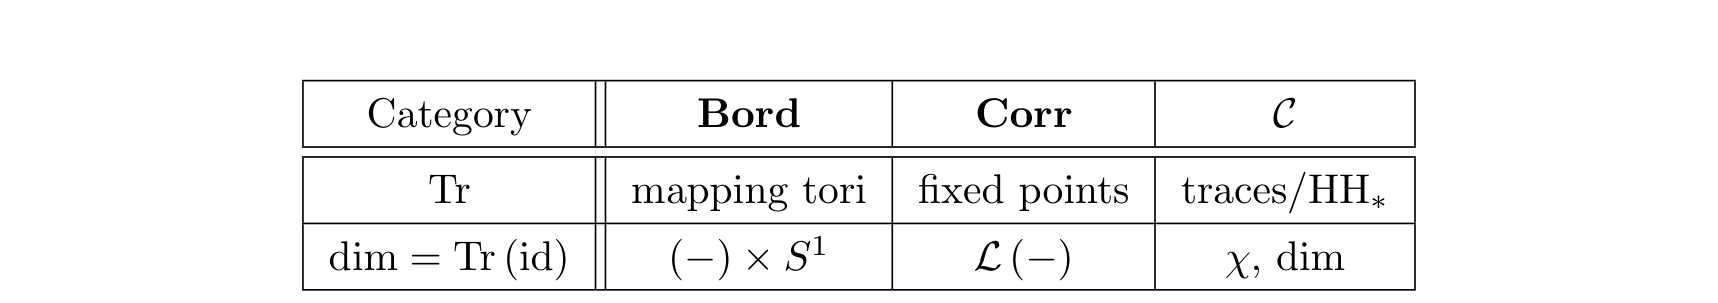
\includegraphics[width=0.68\textwidth]{table12-1.png}
  \caption{$\Bord$、$\mathrm{Corr}$以及 TFT 的目标$\cC$中迹的各种面貌。原文表以图像保留。（原文 p.~216，Table 12.1）}
  \label{tab:12-1}
\end{table}

\begin{srcex}{89}
设$X$是有限集。函数上诱导的映射$f_{*}\colon k(X)\to k(X)$可以看成一个矩阵。于是这个映射的迹是矩阵对角元之和，即$f$的不动点个数。所以经典地，迹来自数不动点。我们稍后会以更精致的说法说明：迹的这种出现与 Lefschetz 不动点公式中的出现是同一回事。
\end{srcex}

总结：若我们的场论$\Bord\to\cC$分解为两个对称幺半函子
\begin{equation}\tag{12.63}
\Bord\to\mathrm{Corr}\to\cC,
\end{equation}
则$\operatorname{Tr}$被保持，而$\operatorname{Tr}$在每个范畴中的面貌如表 12.1 所示。

结论如下。考虑$\mathrm{Corr}$对象上的一个对称幺半的层论，例如
\begin{equation}\tag{12.64}
\Shv\colon\mathrm{Corr}\to\mathrm{Cat},
\end{equation}
它把$X\mapsto\Shv(X)$，并把态射
\begin{equation}\tag{12.65}
\begin{array}{ccc}
 & Z & \\
 p\swarrow & & \searrow q\\
 X & & Y
\end{array}
\end{equation}
送到
\begin{equation}\tag{12.66}
q_{*}p^{!}\colon\Shv(X)\to\Shv(Y).
\end{equation}
注意这只是对应所诱导函子的记号。若我们在这样的设定中，则自动有它把迹送到迹（从而把维数送到维数）。在实践中，我们关心的层论并不平凡地满足这一点。例如我们需要
\begin{equation}\tag{12.67}
\Shv(X\times X)\simeq\Shv(X)\otimes\Shv(X),
\end{equation}
而实践中这有时不成立。

\subsection{与范畴化的关系}\label{sec:12-6-2}

关于迹的整个讨论的结论是：若一个向量空间$V$作为场论$Z$的值出现：
\begin{equation}\tag{12.68}
V=Z\bigl(M\times S^{1}\bigr),
\end{equation}
则我们知道如何范畴化它：
\begin{equation}\tag{12.69}
V=\dim(Z(M)),
\end{equation}
即$Z(M)$范畴化了$V$。或者更一般地，若$V=Z(\text{映射环面})$，则我们有一个自然的视角来范畴化$V$。

% [Tutor Note: (12.51) 在朴素集合层面$\Delta\cap\Delta=\Delta$，真正的信息在导出纤维积：对 orbifold/栈，$X\times_{X\times X}X$记录了对角线的导出自交，这正是“惯性栈”与自由环路空间的区别。(12.67) 的对称幺半性与 §12.6.2 的“迹送到迹”是层论版本的核心假设；在凝聚层或反常层中它通常只在导出意义下成立。]

\section{Lefschetz 不动点公式}\label{sec:12-7}

\begin{sectionkey}
本节从“迹=不动点”出发陈述 Lefschetz 不动点公式与 Grothendieck–Lefschetz 迹公式，并说明它如何给出函数-层对应：层世界中的 Frobenius 迹对应函数世界中的积分，从而把有限群表示论几何化。
\end{sectionkey}

范畴化这一主题在 1990 年代随 Frenkel、Khovanov 与 Baez–Dolan 学派而变得非常流行。但范畴化的想法、以及它的一些更深刻的洞见，可以追溯到 1960 年代 Grothendieck 的工作：Grothendieck–Lefschetz 迹公式。所以几何表示论中的人们从 1970 年代初起就一直在做范畴化，只是没有这么称呼它。

设$X$是拓扑空间，$f\colon X\to X$。回忆 Lefschetz 不动点公式是
\begin{equation}\tag{12.70}
\sum\{\text{不动点}\}=\sum(-1)^{i}\operatorname{tr}\bigl(f|_{H^{i}}\bigr)=\operatorname{Tr}\bigl(f,H^{*}(X)\bigr).
\end{equation}
这个不动点之和等于$\Delta$与$f$的图像的交点个数：
\begin{equation}\tag{12.71}
\sum\{\text{不动点}\}=\#\bigl(\Delta\cap\Gamma_{f}\bigr)=\dim H^{*}\bigl(\Delta\cap\Gamma_{f}\bigr).
\end{equation}
我们必须仔细地数这些不动点，用不同的指数给每个不动点加权（若交点非横截），但这就是公式的一般形状。

如我们所见，取不动点正是几何世界中映射$f\colon X\to X$之迹的正确概念。所以这个公式是在说：上同调把几何范畴中$f\colon X\circlearrowright$的迹送到$X$的上同调上诱导映射的迹。

Grothendieck–Lefschetz 迹公式如下。设$X/\F_q$是有限域上的概形（或栈）。则有
\begin{equation}\tag{12.72}
\#X(\F_{q^{r}})=\operatorname{Tr}\Bigl(F^{r}\big|_{H^{*}_{c}(X,\overline{\Q}_{\ell})}\Bigr),
\end{equation}
其中$F$是 Frobenius 态射，$H^{*}_{c}(-,\overline{\Q}_{\ell})$表示紧支撑$\ell$-进上同调。在道德上，这成立是因为
\begin{equation}\tag{12.73}
\#X(\F_{q^{r}})=\#\bigl(X^{F^{r}}\bigr).
\end{equation}
也就是说，向量空间与自同态
\begin{equation}\tag{12.74}
H^{*}_{c}(X)\circlearrowright F
\end{equation}
范畴化了$\#X(\F_{q})$。

我们可以把$\#X(\F_{q})$看成$X(\F_{q})$上常值函数$1$在映射
\begin{equation}\tag{12.75}
\pi\colon X(\F_{q})\to\mathrm{pt}
\end{equation}
下的前推。即
\begin{equation}\tag{12.76}
\#X(\F_{q})=\pi_{!}1.
\end{equation}
类似地，上同调是$X$上常值层的前推：
\begin{equation}\tag{12.77}
H^{*}_{c}(X)=\pi_{!}\overline{\Q}_{\ell}.
\end{equation}
这就是函数-层对应的诞生。

\begin{srcrem}{88}
我们在$!$前推与$*$前推之间有点马虎。积分中有某种“shriek”的东西，这正是我们前推常值函数时所做的；而我们的上同调是紧支撑的，这也意味着我们应当取$\pi_{!}$。
\end{srcrem}

\subsection{函数-层对应}\label{sec:12-7-1}

\term{函数-层对应}{function-sheaf correspondence}是范畴化更深的概念之一，来自 Weil 猜想。想法是：有一个层的世界，有一个函数的世界。我们说函数，是指在$X(\F_{q})$上的函数。给定一个函数，我们有一个积分操作给出一个数：
\begin{equation}\tag{12.78}
\{X(\F_{q})\text{ 上的函数}\}\xrightarrow{\ \#=\int\ }\R.
\end{equation}
类似地，紧支撑上同调把层变成向量空间：
\begin{equation}\tag{12.79}
\Shv\xrightarrow{\ H^{*}_{c}\ }\Vect.
\end{equation}
但这不只是一个向量空间，而是带 Frobenius $F$的向量空间：
\begin{equation}\tag{12.80}
\Shv\ni E\longmapsto\bigl(V,\ F\colon V\circlearrowright\bigr).
\end{equation}
要从向量空间得到一个数，我们可以取迹：
\begin{equation}\tag{12.81}
(V,F)\longmapsto\operatorname{Tr}(F).
\end{equation}
函数-层对应是说：存在一个从层到函数的迹概念，使得下图交换：
\begin{equation}\tag{12.82}
\begin{array}{ccc}
\{X(\F_{q})\text{ 上的函数}\} & \xrightarrow{\ \#\ } & \R\\
{\uparrow}^{\operatorname{Tr}(F)} & & {\uparrow}^{\operatorname{Tr}(F)}\\
\Shv\ni E & \xrightarrow{\ H^{*}_{c}\ } & \Vect\ni V
\end{array}
\end{equation}
即我们可以在全局化之前或之后取迹。

给定一个数，人们可以把它范畴化为带算子的向量空间，这正是 Lefschetz 公式所说的；然后 Grothendieck 补充说，你可以把这个操作应用到除常值层之外的其他层上，而常值层给出点的个数。从层到函数的操作$\operatorname{Tr}(F)$是
\begin{equation}\tag{12.83}
\operatorname{Tr}(F,E)(x)=\operatorname{Tr}\bigl(F,i_{x}^{*}E\bigr)
\end{equation}
对$x\in X(\F_{q})$。为使之有意义，我们需要$E$是 Weil 层。这意味着它是弱等变的，即我们有同构
\begin{equation}\tag{12.84}
E\xrightarrow{\ \sim\ }F^{*}E.
\end{equation}
于是我们通过在给定点处$E$的 stalk 上取$F$的迹，得到$X(\F_{q})$上的函数。

这是一个例子，说明去范畴化是一个映射（给定层，对每个$r$我们得到$X(\F_{q^{r}})$上的函数），而范畴化是一门艺术。函数-层对应的想法是：有意思的函数来自层。

设$G$是约化群。Lusztig、Kazhdan–Lusztig 与 Deligne–Lusztig 在 80 年代的工作给我们如下口号。有限群$G(\F_{q})$的表示论是几何的，意思是它有范畴化，即它来自把$\operatorname{Tr}(F)$作用于层。这个原理有不同表现形式：该表示论的结构在群$G$及其陪集空间上的层论中有几何起源。这极其重要，例如，若你看有限单群的分类，几乎所有单群都以这种方式出现。所以这些群的特征标可以几何地计算。

\subsection{Lusztig 的特征层}\label{sec:12-7-2}

\term{特征层}{character sheaf}理论确立了：复$G(\F_{q})$-表示的特征标来自$G/G$上的层，即对共轭等变的层。于是从这样一个层出发，我们可以取 Frobenius 的迹得到一个类函数：
\begin{equation}\tag{12.85}
\operatorname{Tr}(F)\colon\frac{G}{G}\to\C\Bigl(\frac{G(\F_{q})}{G(\F_{q})}\Bigr).
\end{equation}

\subsection{Kazhdan–Lusztig 理论}\label{sec:12-7-3}

回忆例 46 中的有限 Hecke 代数：
\begin{equation}\tag{12.86}
\mathcal{H}_{G(\F_{q}),B(\F_{q})}=\overline{\Q}_{\ell}\bigl[B(\F_{q})\backslash G(\F_{q})/B(\F_{q})\bigr],
\end{equation}
即旗簇$G(\F_{q})/B(\F_{q})$上在 Bruhat 轨道上取常值的$\overline{\Q}_{\ell}$值函数。它作为旗簇上函数所给表示的自同态出现：
\begin{equation}\tag{12.87}
\mathcal{H}_{G(\F_{q}),B(\F_{q})}=\End\bigl(\overline{\Q}_{\ell}[G(\F_{q})/B(\F_{q})]\bigr).
\end{equation}
研究它很重要，因为
\begin{equation*}
\mathcal{H}_{G(\F_{q}),B(\F_{q})}\text{-}\mathrm{mod}\subset G(\F_{q})\text{-}\mathrm{mod},
\end{equation*}
即有限 Hecke 代数上的模构成$G$表示论的一部分。具体地，它们是“酉主序列”表示。这覆盖了这个有限群的大部分表示。

Kazhdan–Lusztig 理论说$\mathcal{H}_{G(\F_{q}),B(\F_{q})}$通过范畴化出现，并且用这种方式研究它可以获得深刻洞见。具体地，它说$\mathcal{H}_{G(\F_{q}),B(\F_{q})}$来自$\Shv(B\backslash G/B)$上的$\operatorname{Tr}(F)$：
\begin{equation}\tag{12.88}
\Shv(B\backslash G/B).
\end{equation}
注意现在我们把它看成$\F_{q}$上的概形。人们通常这样说：
\begin{equation}\tag{12.89}
\underbrace{K_0}_{=\dim}\bigl(\Shv(B\backslash G/B)\bigr)=\mathcal{H}_{G(\F_{q}),B(\F_{q})}.
\end{equation}
结论是：我们可以用这一切美妙的几何来研究有限 Hecke 代数。例如，我们在$\Shv(B\backslash G/B)$上有 Verdier 对偶操作，并且在轨道上有由相交上同调层给出的自然自对偶基。这下降为$\mathcal{H}_{G(\F_{q}),B(\F_{q})}$的 Kazhdan–Lusztig 基。这个基有神奇的性质，只要知道这个基，就能重构这个 Hecke 代数的大部分表示论。

这是范畴化帮助你以离开它就做不到的方式理解有限群表示论的一个例子。

% [Tutor Note: (12.72) 中$F^{r}$表示$r$次 Frobenius 迭代，$\overline{\Q}_{\ell}$上的上同调须取紧支撑；$\F_{q^{r}}$是$\F_{q}$的$r$次扩域。(12.84) 的 Weil 层是“弱等变”而非等变——差一个同构而非严格相等，这正是迹依赖$F$的选择的原因。特征层理论要求$G$有足够好的约化结构，且$q$与$\ell$不交。】

\section{几何 Satake}\label{sec:12-8}

\begin{sectionkey}
本节把 Satake 同构看作球 Hecke 代数的范畴化：几何 Satake 对应$\sph\simeq\Rep(G^{\vee})$经$\operatorname{Tr}(F)$去范畴化即得经典的$\mathcal{S}\mathrm{ph}\simeq|\Rep(G^{\vee})|$；区别在于前者用 Tannakian 重构真正构造出$G^{\vee}$，而经典同构只给出表示环。
\end{sectionkey}

几何 Satake 对应大致是说：我们其实没有真正讨论过的 Satake 对应是几何的。Satake 对应是关于球 Hecke 代数的：
\begin{equation}\tag{12.90}
\mathcal{S}\mathrm{ph}=\overline{\Q}_{\ell}\bigl[G(\cO)\backslash G(K)/G(\cO)\bigr].
\end{equation}
这里$K$是局部域。我们可以把它想成 Laurent 级数$K=\F_{q}((t))$或$K/\Q_{\ell}$的有限扩张。我们是在
\begin{equation}\tag{12.91}
\mathcal{S}\mathrm{ph}=\End_{G(K)}\operatorname{Fun}\bigl(G(K)/G(\cO)\bigr)
\end{equation}
遇到它的。回忆我们关心它，是因为它自然地作用在
\begin{equation}\tag{12.92}
\mathcal{S}\mathrm{ph}\circlearrowright\{\text{$G(\F)\backslash G(\bA)/G(\cO_{\bA})$上的函数}\}
\end{equation}
上。所以我们可以把它看成与$G$的局部表示论有关（它是这个表示的自同态），并且它也通过研究自守函数出现在整体图景中。

Hecke 代数一般没有理由交换，但在这种情形我们可以通过范畴化到球 Hecke \emph{范畴}来了解交换性：
\begin{equation}\tag{12.93}
\sph=\Shv\bigl(G(\cO)\backslash G(K)/G(\cO)\bigr),
\end{equation}
这里我们在正特征设定中：$K=\F_{q}((t))$且$\cO=\F_{q}[[t]]\subset K$。去范畴化由 Frobenius 的迹$\operatorname{Tr}(F)$实现：
\begin{equation}\tag{12.94}
\begin{array}{ccc}
\mathcal{S}\mathrm{ph} & \xleftarrow{\ \operatorname{Tr}(F)\ } & \sph
\end{array}
\end{equation}
几何 Satake 对应识别
\begin{equation}\tag{12.95}
\sph\xrightarrow{\ \sim\ }\Rep(G^{\vee})=\QC(\mathrm{pt}/G^{\vee}).
\end{equation}
然后我们可以用$\operatorname{Tr}(F)$去范畴化$\Rep(G^{\vee})$，从而推出经典 Satake 对应。$\QC(\mathrm{pt}/G^{\vee})$上的 Frobenius 就是恒等，至少当群分裂时如此。因此$\operatorname{Tr}(F)=\dim$，它映到表示环：
\begin{equation}\tag{12.96}
|\Rep(G^{\vee})|\xrightarrow{\ \dim\ }\Rep(G^{\vee}).
\end{equation}
但我们知道$\QC$与$\dim$交换，所以我们要计算惯性/环路空间：
\begin{equation}\tag{12.97}
\mathcal{L}(\mathrm{pt}/G^{\vee})=\mathrm{pt}/G^{\vee}\times_{\mathrm{pt}/(G^{\vee}\times G^{\vee})}\mathrm{pt}/G^{\vee}=\frac{G^{\vee}}{G^{\vee}}.
\end{equation}
因此$G^{\vee}$的表示环是$G^{\vee}/G^{\vee}$上的代数函数：
\begin{equation}\tag{12.98}
|\Rep(G^{\vee})|=\cO\Bigl(\frac{G^{\vee}}{G^{\vee}}\Bigr).
\end{equation}
合起来我们得到与函数-层对应中一样的图表：
\begin{equation}\tag{12.99}
\begin{array}{ccc}
\mathcal{S}\mathrm{ph} & \xrightarrow{\ \sim\ } & |\Rep(G^{\vee})|=\cO\Bigl(\frac{G^{\vee}}{G^{\vee}}\Bigr)\\
{\uparrow}^{\operatorname{Tr}(F)} & & {\uparrow}^{\operatorname{Tr}(F)=\dim}\\
\sph & \xrightarrow{\ \sim\ } & \Rep(G^{\vee})
\end{array}
\end{equation}
而最上面一行就是经典 Satake 同构。注意我们也可以把它看成环面上的 Weyl 不变函数：
\begin{equation}\tag{12.100}
\cO\Bigl(\frac{G^{\vee}}{G^{\vee}}\Bigr)=\cO(H^{\vee})^{W}.
\end{equation}
这有用的一种方式是：我们对范畴$\sph$交换有一个很好的理由，而现在这表明 Hecke 代数$\mathcal{S}\mathrm{ph}$也交换。也许更深刻的是：Langlands 对偶群$G^{\vee}$出现了。所以 Satake 同构的 Langlands 解释是
\begin{equation}\tag{12.101}
\mathcal{S}\mathrm{ph}\simeq|\Rep(G^{\vee})|,
\end{equation}
其中$G^{\vee}$是$\C$上的约化群，其根数据对偶于$G$的根数据。但我们不能从$|\Rep(G^{\vee})|$恢复$G^{\vee}$：群一般不由其表示环决定。然而几何 Satake 对应实际上用 Tannakian 重构为我们构造了对偶群$G^{\vee}$。这是几何 Satake 对应比经典版本更强大的众多原因之一。

% [Tutor Note: (12.90) 与 (12.93) 中$\mathcal{S}\mathrm{ph}$（代数）与$\sph$（范畴）用不同字体区分，原文用粗体与花体混排、容易混淆；这里统一以$\mathcal{S}\mathrm{ph}$记球 Hecke 代数、$\sph$记球 Hecke 范畴。(12.97) 的$\mathcal{L}$是惯性/自由环路空间；对$\mathrm{pt}/G^{\vee}$它等于$G^{\vee}/G^{\vee}$，故$\QC$的维数给出$G^{\vee}$的表示环而非群本身——这正是 Tannakian 重构（保留张量结构）比$K_0$（只看表示环）更强的地方。]


\chapter{Langlands 对应}\label{ch:13}

\begin{keytakeaways}
本章把几何 Langlands 纲领翻译为算术语言。物理图像是四维规范理论 $\cA_G$ 与它的电磁对偶 $\cB_{G^\vee}$：把三维流形换成函数域或数域，把纽结换成素点，则’t~Hooft 线算子（在 $G$ 一侧由 $\Rep(G^\vee)$ 标号）应被 Wilson 线算子（在 $G^\vee$ 一侧由局部系统标号）实现。由此得到非分歧 Langlands 对应的谱分解猜想：自守形式层沿 $\Loc_{G^\vee}(C)$ 分解，且应为对偶层 $\omega$。分歧情形需要引入局部 Langlands 对应——它正是“某条特定曲线上的几何 Langlands”，在导出意义下表现为平滑表示范畴与 $\QC(\Loc_{G^\vee})$ 之间的等价（或其全子范畴），而 $L$-函数是把两侧的数值数据（Hecke 特征值与 Frobenius 特征值）粘合起来的“神奇胶水”。
\end{keytakeaways}

\section{几何 Satake}\label{sec:13-1}

\begin{flushright}\small 第 31 讲；2021 年 6 月 3 日\end{flushright}

\begin{sectionkey}
本节的核心是：几何 Satake 就是“线算子”版本的对偶性——这个“自守 TFT”中 $S^2$ 上的线算子所成的范畴，同构于 Langlands 对偶群的表示；而把它降到 $S^2\times S^1$ 上做范畴化/去范畴化，就得到表示环 $|\Rep(G^\vee)|$。
\end{sectionkey}

回忆我们可以用这个“自守 TFT”中的线算子，也就是赋值 $\cA_G(S^2)$，来表述几何 Satake。于是几何 Satake 说，它可以与 Langlands 对偶的表示等同起来：
\begin{equation}\tag{13.1}
\left(\cA_G(S^2),*\right)\simeq \Rep(G^\vee).
\end{equation}

事实上，这正是我们对 $G^\vee$ 的定义。回忆一下，从物理上看，$\cA_G(S^2)$ 由 't~Hooft 线算子构成，所以它们是这个四维规范场论的一维缺陷。它们是 Dirac 单极子的一种推广。我们在电磁学中见过这些：四维中有一条单极子的世界线，而规范场被允许在其上有奇点。所以，如果我们有四维中的一条线，其链环是一个二维球面，而在 $S^2$ 上给定一个丛、或者更确切地说给定它的 Chern 类，就是在给定单极子本身的电荷。

在交换情形，电荷是一个整数，但现在电荷是表示环 $|\Rep(G^\vee)|$ 中的一个元素。还有更具体的东西，类似于交换情形中所见的，那就是 't~Hooft 圈算子。给定四维流形中的一个圈，它的链环现在是 $S^2\times S^1$，于是 $\cA_G(S^2\times S^1)$ 的元素就是圈的可能的“标号”。由我们关于范畴化的讨论，现在我们知道：
\begin{align}
\cA_G(S^2\times S^1)&=\dim\cA_G(S^2) \tag{13.2}\\
&=|\Rep(G^\vee)|. \tag{13.3}
\end{align}
所以，经典地看，'t~Hooft 单极子是放在四维中一个闭圈上的东西，用一个对偶群 $G^\vee$ 的表示来标记；但现在它只是一个由表示构成的向量空间。
% [Tutor Note: 源文此处写作“$\cA_G(S^2\times S^2)$ 的元素就是圈的可能的标号”，与同一句前半的链环 $S^2\times S^1$ 矛盾，应为 $S^2\times S^1$（即 (13.2) 左端）。译文按上下文取 $S^2\times S^1$，并在此标明原文笔误。]

这实际上就是下述情形中出现的东西。如果我们在三维流形 $M^3$ 上研究这个理论，就得到某个向量空间 $\cA_G(M^3)$。而如果给我某个纽结 $K\subset M^3$ 以及标号 $V\in|\Rep(G^\vee)|$，那么我们就能构造一个单极子算子，它作用在向量空间 $\cA_G(M^3)$ 上。这些就是 't~Hooft 圈算子。表示 $V\in|\Rep(G^\vee)|$ 也标记了简单得多的 $B$-理论 $\cB_{G^\vee}$ 中的 Wilson 圈。回忆这个理论研究三维流形上的平坦 $G^\vee$-联络。给定一个平坦 $G^\vee$-联络与一个纽结 $K\subset M^3$，有一个经典可观测量的算子叫做 Wilson 圈算子，它沿纽结 $K$ 取平坦联络在表示 $V$ 中的和乐的迹。所以这定义了局部系统空间 $\Loc_{G^\vee}(M^3)$ 上的一个函数。
% [Tutor Note: (13.1) 左端的 $*$ 是线性对偶，不是范畴化意义下的对偶；书中用它强调 $\cA_G(S^2)$ 是“线算子所成范畴”在某种意义下的 $K_0$ 型不变量。(13.2)--(13.3) 用到了配边假设：$S^2\times S^1$ 是 $S^2$ 上的圆族，取“圆上的迹”给出 $\dim$。切勿把 $\dim\cA_G(S^2)$ 理解为向量空间维数，它是范畴的迹（即去范畴化后的维数）。]

% [Tutor Note: 物理侧的对应是：'t~Hooft 算子的电荷原本是 $H^2(S^2;\Z)=\Z$（交换情形），非交换情形应取在 $\Rep(G^\vee)$ 中；“表示环元素”只是其 $K_0$ 影子。真正的标号在导出/范畴化层面是一个 $\Rep(G^\vee)$-模结构，这也解释了为什么后面要出现 $|\Rep(G^\vee)|$ 与 $\Rep(G^\vee)$ 两个层次。]

\section{函数域上的非分歧 Langlands 对应}\label{sec:13-2}

\begin{sectionkey}
本节把 $M^3$ 换成函数域（或数域），把纽结换成素点，得到非分歧情形：$|\Rep(G^\vee)|$ 在每个点上通过 Hecke 算子作用在自守形式上；问题变成这个作用是否沿 $\Loc_{G^\vee}(C)$ 分解（层化），以及分解后是哪个模。
\end{sectionkey}

在 Langlands 纲领中，我们将用别的对象来替代三维流形 $M^3$，让它们扮演三维流形的角色。如我们已见，可以把 $M$ 替换为：
\begin{enumerate}
\item 有限域上的曲线 $C/\F_q$，以及
\item 数域 $F$，即 $\Q$ 的有限扩张。
\end{enumerate}

Langlands 对应最重要的特征是代数 $|\Rep(G^\vee)|$ 在作用。代替纽结 $K\subset M^3$，我们在第一种情形中有某个点 $x\in C(\F_q)$，在第二种情形中有一个素理想 $\mathfrak p\in\cO_F$。回忆表示环来自对几何 Satake 对应的去范畴化。我们也看到它来自一种更精细的去范畴化。也就是说，我们看到 $|\Rep(G^\vee)|$ 作为 Frobenius 的迹 $\mathrm{Tr}(F)$ 出现在
\begin{equation}\tag{13.4}
\sph=\Shv\bigl(G(\cO)\backslash G(K)/G(\cO)\bigr)
\end{equation}
上。为了让 Frobenius 有意义，我们要设想例如
\begin{equation}\tag{13.5}
K=\F_q(\!(t)\!)\supset \F_q[\![t]\!]=\cO.
\end{equation}
结果得到的是函数而不是层：
\begin{equation}\tag{13.6}
\sph=|\sph|=\mathrm{Fun}\bigl(G(\cO)\backslash G(K)/G(\cO)\bigr).
\end{equation}
说了这么多，无非是在说经典的 Satake 同构断言：
\begin{equation}\tag{13.7}
\cH_{G(K),G(\cO)}\simeq|\Rep(G^\vee)|.
\end{equation}
事实上，经典 Satake 对 $K=\F_q(\!(t)\!)$ 或 $K$ 为 $\Q_p$ 的有限扩张（混合特征局部域）时同样成立。

现在回忆我们为什么经典地研究这个 Hecke 代数。回忆我们有这个等同：
\begin{align}
\Bun_G(C)&\simeq G(F)\backslash G(\bA_F)/G(\cO_{\bA}) \tag{13.8}\\
&=G(F)\backslash {\prod}' G(K_x)/G(\cO_x). \tag{13.9}
\end{align}
也就是说，它是仿射 Grassmann 簇 $G(K_x)/G(\cO_x)$ 的乘积再模掉这个巨大的整体部分 $G(F)$。因为可以这样写，这意味着它有一个对称性。即：这个空间上的函数
\begin{equation}\tag{13.10}
\mathrm{Aut}_C:=\mathrm{Fun}_c(\Bun_G(C))
\end{equation}
自动带有球 Hecke 代数 $|\sph|$ 在每个点 $x\in C$ 上的作用。换句话说，张量积作用在 $\mathrm{Aut}_C$ 上：
\begin{equation}\tag{13.11}
\bigotimes'_{x\in C}|\Rep(G^\vee)|\ \curvearrowright\ \mathrm{Aut}_C.
\end{equation}

\begin{srcrem}{89}
这是处处非分歧的情形。要得到分歧版本，我们还得做一番工作。
\end{srcrem}

在这个设定下，Langlands 对应说的是下面这件事。我们有一个向量空间 $\mathrm{Aut}_C$ 带着这个巨大的作用。想法是试着把它与某个具有同样对称性的东西匹配起来。我们还知道别的带有这个巨大作用的向量空间吗？再一次，我们应该想到 Wilson 圈：每当你自然地看到由群表示标号的函数，若你看平坦联络空间，那么每当你看到一个圈，就可以取这个 Wilson 函数。所以考虑空间
\begin{equation}\tag{13.12}
\Loc_{G^\vee}(C)=\{\Gal(F)\to G^\vee\}/G^\vee,
\end{equation}
其中右端按共轭取商，而且我们其实应该想 $F$ 的 Weil 群而非 Galois 群，意思是应把 Frobenius 当作生成一个 $\Z$ 的拷贝（而不是 $\widehat{\Z}$）。这里有些微妙之处，例如它显然不是一个代数簇。无论如何，对每个点 $x\in C$，有一个自然映射
\begin{equation}\tag{13.13}
\Loc_{G^\vee}(C)\to \frac{G^\vee}{G^\vee}.
\end{equation}
也就是说，我们可以把与这个表示有关的一切都忘掉，只保留与 $x\in C$ 相应的 Frobenius $F_x$ 的像。即
\begin{equation}\tag{13.14}
\rho\mapsto \rho(F_x).
\end{equation}
对偶地，这个映射等价于一个映射
\begin{equation}\tag{13.15}
\cO\left(\frac{G^\vee}{G^\vee}\right)=|\Rep(G^\vee)|\to\cO\bigl(\Loc_{G^\vee}(C)\bigr),
\end{equation}
而这正是我们先前所称的 Wilson 圈。

所以换句话说，$\mathrm{Aut}_C$ 与 $\cO(\Loc_{G^\vee}(C))$ 都带有这个巨大张量积的作用：
\begin{equation}\tag{13.16}
\mathrm{Aut}_C\ \curvearrowleft\ \bigotimes'_{x\in C}|\Rep(G^\vee)|\ \curvearrowright\ \cO\bigl(\Loc_{G^\vee}(C)\bigr).
\end{equation}
在右边，我们其实只有一个同态，作用只来自乘法。在左边，它来自这些卷积/Hecke 算子。于是我们找到了某个与自守形式空间 $\mathrm{Aut}_C$ 具有同样对称性的东西，现在可以问：

\medskip\noindent\textbf{问题 8.} $\mathrm{Aut}_C\simeq\cO(\Loc_{G^\vee}(C))$？

在问它是否为同构之前，我们可以先问下面这件事。同样，$\cO(\Loc_{G^\vee}(C))$ 上的作用其实来自一个同态：
\begin{equation}\tag{13.17}
\bigotimes'_{x\in C}|\Rep(G^\vee)|\to\cO\bigl(\Loc_{G^\vee}(C)\bigr).
\end{equation}
所以我们首先可以问，这个作用是否分解为
\begin{equation}\tag{13.18}
\begin{array}{ccc}
\mathrm{Aut}_C & & \cO\bigl(\Loc_{G^\vee}(C)\bigr)\\[6pt]
& \nwarrow\ \bigotimes'_{x\in C}|\Rep(G^\vee)|\ \nearrow &
\end{array}
\end{equation}
% [Tutor Note: (13.18) 的交换三角形在原书中以手绘箭头给出（p.~223），此处以 array 重排：底部的张量积同时映到 $\mathrm{Aut}_C$（经由 Hecke/卷积算子）与 $\cO(\Loc)$（经由 Wilson 圈）。问题在于这后一个映射是否“穿过” $\mathrm{Aut}_C$。]
% [Tutor Note: (13.15) 中把 $\cO(G^\vee/G^\vee)$ 与 $|\Rep(G^\vee)|$ 等同，依赖 $G^\vee$ 是约化群、$\cO(G^\vee)^{G^\vee}=\cO(G^\vee/G^\vee)$ 为不变函数环；这是 GIT 商而非栈商，见 (13.60) 的讨论。]

于是我们可以问：这些表示环在每一点的作用，是否“协调成”曲线上的局部系统之中它们所满足的同样关系？换句话说，我们在问下面这件事。

\medskip\noindent\textbf{问题 9.} $\mathrm{Aut}_C$ 是否在 $\Loc_{G^\vee}(C)$ 上层化/谱分解？即，\emph{A}-侧是否在 \emph{B}-侧上层化？

答案是肯定的。这就是“Langlands 对应的自守到 Galois 方向”，由 Vincent Lafforgue 证明。更抽象的证明见 [AGK$^+$20b, AGK$^+$20a, AGK$^+$21]。

既然我们有了这个层化，我们可以问：这是哪一个模？这仍然是公开问题，但我们至少可以作出猜想，如 [AGK$^+$20b, AGK$^+$20a, AGK$^+$21] 中所述。

\begin{srcconj}{1（函数域上的非分歧 Langlands 对应）}
作为 $\Loc_{G^\vee}(C)$ 上的层，
\begin{equation}\tag{13.19}
\mathrm{Aut}_C\simeq\omega\bigl(\Loc_{G^\vee}(C)\bigr).
\end{equation}
\end{srcconj}

\begin{srcrem}{90}
$\omega$ 表示对偶层。要点是：聪明的做法是取体积形式而不是函数。这类似于取 $\QC$ 与取 $\IndCoh$ 之间的差别。
\end{srcrem}
% [Tutor Note: (13.19) 用 $\omega$ 而非 $\cO$是本章的技术核心之一：在光滑栈上 $\omega$ 是“体积形式/对偶复形”，其函子性（pushforward）比函数环好；若误写成 $\mathrm{Aut}_C\simeq\cO(\Loc)$，则在分歧点处无法得到正确的上同调支撑（参见 (13.117) 中 $\cO$-mod $\ne\QC$ 的现象）。“$\omega$ 版本”也解释了为什么 (13.118) 中要用 $\IndCoh$ 而不是 $\QC$。]

\section{分歧 Langlands 对应}\label{sec:13-3}

\begin{sectionkey}
本节从非分歧情形过渡到分歧情形：自守侧把 $\Bun_G(C)$ 换成带层结构的 $\Bun_G(C,S)$，谱侧把 $\Loc_{G^\vee}(C)$ 换成 $\Loc_{G^\vee}(C\setminus S)$；在 $S$ 之外谱分解仍成立（V.~Lafforgue 定理），但在 $S$ 处到底“是什么层”需要局部 Langlands 对应来回答。数域情形还说明为什么需要 Langlands 群。
\end{sectionkey}

我们之所以需要转到分歧情形，原因之一是要容纳 Langlands 对应真正的/原本的设定，那里我们有数域（而不是三维流形或函数域）。\term{分歧}{ramification}大致上是指从朴素的丛过渡到在某些点处带有额外数据的丛。在数域情形中，根本不存在处处非分歧设定的版本：无穷素点总是看起来与别的素点不同，于是曲线上总有一个点与所有别的点看起来不一样。

当我们谈论分歧时，大致有两个阶段/世代：一个预备步骤和一个更精细的步骤。在第一步中我们基本上忽略 $S$，即试图理解在我们丛带有额外结构的特殊点之外发生了什么。第二步则是让我们放大到某个分歧点附近，试图理解那里在发生什么。这就是局部 Langlands 对应。

\subsection{自守侧的分歧}\label{sec:13-3-1}

当我们在自守侧过渡到分歧情形时，代替 $\Bun_G(C)$，我们考虑
\begin{equation}\tag{13.20}
\Bun_G(C,S),
\end{equation}
其中 $S$ 是 $C$ 的有限子集；而 $\Bun_G(C,S)$ 由在 $S$ 中各点处带有某些额外结构的丛构成。

更精确地说，我们可以用阿黛尔式的描述来写它。回忆我们有
\begin{equation}\tag{13.21}
\Bun_G(C)=G(F)\backslash G(\bA)/\prod_{x\in S}G(\cO_x).
\end{equation}
% [Tutor Note: 源文此处写作 $\prod_{x\in S}$，与紧接着的“在右边少模掉一些”以及 (13.22) 中的 $\prod_{x\notin S}G(\cO_x)\times\prod_{x\in S}K_x$ 相矛盾：右端应为对全部 $x\in C$ 的乘积，或至少 $\prod_{x\notin S}$。此处照译原文并标明，读者应按 (13.22) 理解。]
于是现在我们在右边模掉更少的东西，得到
\begin{equation}\tag{13.22}
\Bun_G(C,S)=G(F)\backslash G(\bA)\Big/\left(\prod_{x\notin S}G(\cO_x)\times\prod_{x\in S}K_x\right),
\end{equation}
其中 $K_x\subset G(\cO_x)$。如果我们在右边什么都不模掉，即取 $G(F)\backslash G(\bA)$，那么它由在每个点 $x\in C$ 附近都有平凡化的丛构成。

一旦我们用这种方式表述了函数域情形，就有一个自然的数域类比。对 $F$ 为数域，我们写
\begin{align}
[G]_F&=G(F)\backslash G(\bA) \tag{13.23}\\
[G]_{F,K_S}&=G(F)\backslash G(\bA)\Big/\left(\prod_{\mathfrak p\notin S}G(\cO)\times\prod_{\mathfrak p\in S}K_{\mathfrak p}\right), \tag{13.24}
\end{align}
其中 $S$ 是包含无穷素点的一族素点。

在这个设定中，自守形式是 $[G]_{F,K_S}$ 上的函数（数域情形中为 $L^2$ 函数），并且称 $K_S$ 为该自守形式的级。

\subsection{谱侧}\label{sec:13-3-2}

于是在分歧的故事里，我们在函数域设定中有自守形式
\begin{equation}\tag{13.25}
\mathrm{Aut}_{C,S,K_S}=\mathrm{Fun}_c\,\Bun_G(C,K_S),
\end{equation}
而在数域设定中有
\begin{equation}\tag{13.26}
\mathrm{Aut}_{F,S,K_S}=L^2\bigl([G]_{F,K_S}\bigr).
\end{equation}
接着我们可以问：什么在作用？

\begin{srcrem}{91}
其物理图像如下。考虑一个 Riemann 面 $C$。那么 $\Bun_G(C,K_S)$ 由在这些点处带有某些数据的丛构成。从物理的观点看，我们把点 $x\in C$ 看作四维中的余维 2 奇点。于是我们有面缺陷/螺线管（solenoid）。分歧的这个初步的、暂时不加区分的阶段（即当我们看向 $S$ 之外时），我们并不指定这些点处发生了什么，因为我们只想在 $S$ 之外重复先前的做法。

在 $S$ 之外，我们仍有同样的局部因子，即它仍看起来像对 $x\in S$ 的 $G(K)/G(\cO)$ 的乘积，然后我们仍在左边用这个整体群 $G(F)$ 取商。
% [Tutor Note: 源文此处写“对 $x\in S$ 的乘积”，与同一句开头的“在 $S$ 之外”以及紧接着的“对 $x\notin S$ 我们仍得到同一个 Hecke 代数的作用”自相矛盾，应为 $\prod_{x\notin S}G(K_x)/G(\cO_x)$；此处照译原文并标明，读者不要据此认为分歧会改变 $S$ 之外的局部因子。[译者按（无外部依据）]]
\end{srcrem}

代数地说，这是在说对 $x\notin S$ 我们仍得到同一个 Hecke 代数的作用：
\begin{equation}\tag{13.27}
\cH_{G(K),G(\cO)}=|\Rep(G^\vee)|.
\end{equation}

\paragraph{函数域}
暂时限制到函数域设定（我们将在下一小节回到数域设定），这是在说 $\mathrm{Aut}_{C,S}$ 带有这个巨大的（限制）张量积的作用：
\begin{equation}\tag{13.28}
\bigotimes'_{x\notin S}|\Rep(G^\vee)|\ \curvearrowright\ \mathrm{Aut}_{C,S}.
\end{equation}
现在我们可以问与先前相同的问题：这个代数还在哪里出现？即，什么东西与 $\mathrm{Aut}_{C,S}$ 具有同样的对称性？先前那类图像自然再次出现。也就是说，有一个自然的环的商映射
\begin{equation}\tag{13.29}
\bigotimes_{x\notin S}|\Rep(G^\vee)|\twoheadrightarrow\cO\bigl(\Loc_{G^\vee}(C\setminus S)\bigr),
\end{equation}
而且我们可以问这个作用是否分解为
\begin{equation}\tag{13.30}
\begin{array}{ccc}
\mathrm{Aut}_{C,S} & & \cO\bigl(\Loc_{G^\vee}(C\setminus S)\bigr)\\[6pt]
& \nwarrow\ \bigotimes_{x\notin S}|\Rep(G^\vee)|\ \nearrow &
\end{array}
\end{equation}
也就是说，在 $S$ 之外我们得到与先前相同的谱分解。这同样是 V.~Lafforgue 的定理：对任何级结构 $K_S$，$\mathrm{Aut}_{C,S}$ 都沿 $\Loc_{G^\vee}(C\setminus S)$ 层化。
% [Tutor Note: (13.29) 左端用的是不带撇的 $\bigotimes$（原文如此），而 (13.28) 用的是限制张量积 $\bigotimes'$；两者在“限制”意义下的区别是源文的记号疏漏，不影响实质。]

所以这些局部系统被允许在 $S$ 处分歧。在非分歧点，局部 Galois 群 $\Gal(F)$ 通过一个小商 $\Z\langle F\rangle$ 作用，即由 Frobenius 生成的一个 $\Z$ 的拷贝。在分歧点，我们可能有绕该点的复杂单值。所以在 $S$ 中的点上，我们并不对作用是否通过这个小商分解作任何断言。

\begin{srcrem}{92}
这是一个惊人的定理，但我们其实并不知道它究竟是哪一个层。要把它钉死，我们真的需要理解分歧点处发生了什么，而这正是局部 Langlands 对应的主题。
\end{srcrem}

\paragraph{数域}
现在我们回到数域设定。设 $[F:\Q]<\infty$ 为 $\Q$ 的有限扩张。那么我们有这个自守形式空间 $\mathrm{Aut}_{F,S,K_S}$，它依赖于 $F$、有限素点集 $S$ 以及某个级结构 $K_S$。它带有
\begin{equation}\tag{13.31}
\bigotimes'_{\mathfrak p\notin S}|\Rep(G^\vee)|
\end{equation}
的作用，我们也许会期待同样的答案。结果发现，同样的答案是不对的。我们或许会猜：考虑某个版本的 Galois 群，并看同态的共轭类
\begin{equation}\tag{13.32}
\{\Gal_F\to G^\vee\}/G^\vee.
\end{equation}
然后我们或许曾希望从限制张量积到该空间上的函数有一个映射
\begin{equation}\tag{13.33}
\bigotimes'_{\mathfrak p\notin S}|\Rep(G^\vee)|\to\cO\bigl(\{\Gal_F\to G^\vee\}/G^\vee\bigr),
\end{equation}
并使作用分解。结果这并不正确：它不分解。

Langlands 提出了一个猜想性的群的定义，称为 $F$ 的 Langlands 群 $\mathrm{Lang}_F$，使得一旦把 Galois 群替换成 Langlands 群，上述图像就成立。于是应该有一个映射
\begin{equation}\tag{13.34}
\mathrm{Lang}_F\to\Gal_F,
\end{equation}
于是我们该看同态
\begin{equation}\tag{13.35}
\mathrm{Lang}_F\to G^\vee.
\end{equation}
有些会通过 $\Gal(F)$ 分解，但不是全部。所以我们需要一个更大的参数空间。

\begin{srcrem}{93}
这也是为什么很难把 Langlands 对应的陈述钉死的原因之一：它涉及某个尚未被完全定义的 Galois 群版本的表示。
\end{srcrem}

另一个视角是：在这些自守形式空间内部，还有更小的空间：
\begin{equation}\tag{13.36}
\begin{array}{c}
\text{自守形式}\\[2pt]
\uparrow\\[2pt]
\text{代数自守形式}\\[2pt]
\uparrow\\[2pt]
\text{上同调自守形式}
\end{array}
\end{equation}
这些空间比全部自守形式空间更易处理，但它们仍然捕获了人们关心 Langlands 对应的大部分理由。粗略地说，与普通自守形式的区别是 $L^2([G]_F)$ 被换成 $H^*([G]_F)$，可能带扭系数。例如我们可能看 $H^*(\Gamma\backslash G_\R/K)$ 而不是该空间上的 $L^2$ 函数，而这基本上就是群上同调 $H^*(\Gamma)$。我们不会详细讨论代数自守形式，但粗略地说，全部自守形式与代数/上同调自守形式的区别是在 $\infty$ 素点处的一个条件。

然后还有所谓的 Clozel 猜想，它是 Langlands 猜想的一个版本。

\begin{srcconj}{2 (Clozel)}
代数自守形式对应于 Galois 表示。
\end{srcconj}

即，如果我们在 $\mathrm{Aut}_{F,S}$ 上加一个条件，就得到与先前类似的图像：
\begin{equation}\tag{13.37}
\begin{array}{ccc}
\mathrm{Aut}^{\mathrm{alg}}_{F,S} & & \cO\bigl(\{\Gal_F\to G^\vee\}/G^\vee\bigr)\\[6pt]
& \nwarrow\ \bigotimes'_{\mathfrak p\notin S}|\Rep(G^\vee)|\ \nearrow &
\end{array}
\end{equation}
我们仍在某种程度上把东西扫到地毯下面，因为我们需要谈论 $\ell$-进表示，而我们还没有指定 $\ell$。解决办法是：不只考虑 Galois 表示 $\Gal\to G^\vee$，而是对所有 $\ell$ 取相容的 $\ell$-进 Galois 表示族。这是人们所称的动机（motive）的一个版本。等价地，Clozel 猜想处理的是某种 Motivic Galois 群的表示。应当记住的经典图像是：我们有例如模形式的 $L$-函数，它们属于 $\mathrm{Aut}^{\mathrm{alg}}_{F,S}$；而在另一侧应该想椭圆曲线，它们给出 Motivic Galois 表示。
% [Tutor Note: (13.37) 与 (13.18)、(13.30) 同型：三角形说明 “大张量积同时作用在自守侧与谱侧”，而 Clozel 猜想断言的是“作用穿过自守侧”——但仅在代数自守形式的全子范畴上。原文图以手绘箭头给出（p.~227），此处重排。]
% [Tutor Note: 代数自守形式（algebraic automorphic forms）与上同调自守形式的区别不容混淆：前者要求无穷素点处的无穷小特征属于某个格（即“代数”），后者要求出现在 $H^*([G]_F)$ 中；Clozel 猜想通常陈述为上同调自守形式（或代数自守形式的有理结构）对应 Galois 表示。]

\begin{srcrem}{94}
当我们考虑 $[G]_F$ 上的函数时，需要指定它们取值于哪个域 $k$。当我们考虑 Galois 表示 $\Gal(F)\to G^\vee$ 时，群 $G^\vee$ 定义在同一个域 $k$ 上。为简单起见取 $G^\vee=\mathrm{GL}_n$。于是我们在考虑表示
\begin{equation}\tag{13.38}
\Gal(F)\to \mathrm{GL}_n(k),
\end{equation}
问题在于 Galois 群是投射有限群，即一种拓扑群。而对拓扑群的表示唯一合理的概念是连续表示。我们或许会猜可以简单地取 $k=\C$，但 $\Gal(F)$ 与 $\C$ 的拓扑并不协调：唯一的连续表示 $\Gal(F)\to\mathrm{GL}_n(\C)$ 是像为有限的表示。这已经很重要（这是 Artin 猜想的故事），但它们并不覆盖我们感兴趣的全部表示。例如来自椭圆曲线的表示不是有限像表示。事实上，来自代数几何的有限像表示只来自零维簇的上同调。

要得到更多表示，我们应寻找取值于类似 $\mathrm{GL}_n(\overline{\Q}_\ell)$ 的东西中的表示。当然 $\overline{\Q}_\ell$ 同构于 $\C$，但它带有某种拓扑，于是这些 $\ell$-进 Galois 表示不再被要求有有限像。但现在我们有一些额外的复杂性。例如，如果表示来自 $\F_p$ 上代数簇的上同调，那么可能有 $\ell=p$，这需要单独处理。于是问题变成：$\ell$ 是什么？在局部情形，即我们只有一个 $p$ 时，我们可以简单地取 $\ell\neq p$。但如果我们在做整体的事情，即试图一次处理所有素数，那么我们不能选一个与所有素数 $p$ 都不同的 $\ell$。所以我们被引向相容表示族的概念。即，与其考虑单个 $\ell$-进表示，不如考虑对所有 $\ell$ 的一族相容的 Galois 表示。

这看起来是个奇怪的概念，但它来自代数几何。设 $X$ 是一个概形。那么我们可以试着定义它的上同调。于是我们需要选一个系数域。结果并不存在一个带有理系数的好的代数上同调理论。即，不存在一个落在 $\Q$-向量空间中的、满足适当条件的函子。但我们可以对每个 $\ell$ 用 $\Q_\ell$ 来做。每一个都带有 $\Gal$ 的作用，于是我们对每个 $\ell$ 都有一个。所以实际上我们有一族对全体素数 $\ell$ 的 $\ell$-进 Galois 表示（或者若 $X/\F_p$ 则 $\ell\neq p$）。我们真正想研究的其实是 $X$ 的某种 Motivic 上同调 $H^*_M(X)$，它是某种 $\Q$-向量空间。它实际上并不存在，但它是某个 $\Q$-线性范畴中的一个良定义对象，该范畴称为动机范畴。于是给定一个动机和一个素数 $\ell$，通过取 $\ell$-进平展上同调，我们得到 $\Q_\ell$-向量空间。
\end{srcrem}
% [Tutor Note: 这一段是全书对“动机”最直白的解释：单个 $\ell$-进表示是实现，动机才是“对所有 $\ell$ 一致的母对象”。技术上 $H^*_M(X)$ 应理解为一个 Chow 型动机（或至少是 numerical/homological 动机）中的对象，其各种实现（de Rham、Betti、$\ell$-进平展）是纤维函子；把它当成真实存在的 $\Q$-向量空间会出错。]

\section{L-函数}\label{sec:13-4}

\begin{sectionkey}
本节把谱分解具体化：Hecke 特征值给出一族共轭类 $F_{\mathfrak p}\in G^\vee/\!/G^\vee$，而 $L$-函数正是用特征多项式（$\det(1-p^{-s}F_{\mathfrak p})$ 的倒数）把这些数值数据打包起来。于是 Langlands 对应可以“粗”地表述为：自守形式与 Galois 表示在 $L$-函数相等时相匹配。
\end{sectionkey}

从同样的初始数据出发，我们还能做更具体的事情。我们有一个自守形式空间 $\mathrm{Aut}$，带有这个整体 Hecke 代数的作用：
\begin{equation}\tag{13.39}
\mathcal{H}\mathrm{ecke}=\bigotimes'_{\mathfrak p\notin S}|\Rep(G^\vee)|.
\end{equation}
谱分解只是对角化的花哨说法。所以当我们做谱分解时，首先可以要求的是 Hecke 特征函数。自守形式 $f\in\mathrm{Aut}$ 尤其是所有 Hecke 算子的联合特征函数。\footnote{还有一些额外的解析增长条件，我们不重点关注。}我们可以问的一件事是，如何刻画 $\mathrm{Hecke}$ 作用在 $\mathrm{Aut}$ 上的特征值。技术上它是一个特征，即同态
\begin{equation}\tag{13.40}
\mathcal{H}\mathrm{ecke}\to k.
\end{equation}
但这不太具体。回忆
\begin{equation}\tag{13.41}
\mathcal{H}\mathrm{ecke}=\bigotimes \cO\left(\frac{G^\vee}{G^\vee}\right).
\end{equation}
% [Tutor Note: (13.41) 右端的 $\bigotimes$ 在原文中没有下标，应为 (13.39) 中的 $\bigotimes'_{\mathfrak p\notin S}$；这是源文记号疏漏。这里照译。]
% [Tutor Note: (13.39)--(13.41) 的 $\mathcal{H}\mathrm{ecke}$ 是同一个整体 Hecke 代数的同一书写，不是两个不同的环；花体的 $\mathcal{H}$ 只是作者对该代数的写法。[译者按（无外部依据）]]
我们可以取 $G^\vee$ 上不变函数的一组基，并试着用这组基描述这些算子的特征值。但有一个更优雅的进路。设 $G^\vee$，或者更一般地，选一个同态
\begin{equation}\tag{13.42}
V:\ G^\vee\hookrightarrow \mathrm{GL}_n.
\end{equation}
它对应于一个映射
\begin{equation}\tag{13.43}
\bigotimes\cO\left(\frac{\mathrm{GL}_n}{\mathrm{GL}_n}\right)\to\bigotimes\cO\left(\frac{G^\vee}{G^\vee}\right).
\end{equation}
现在我们把问题变成了关于 $\mathrm{GL}_n$ 上类函数的问题。每个人都有一个衡量矩阵的最爱方式，那就是特征多项式。这就是为什么我们把问题翻译成 $\mathrm{GL}_n$ 的语言：任意的 $G^\vee$ 没有明确的方式编码一个元素的信息。设 $F\in\mathrm{GL}_n$。那么我们附上\emph{\term{特征多项式}{characteristic polynomial}}，即
\begin{equation}\tag{13.44}
\det(1-tF).
\end{equation}
更花哨的说法是：我们看 $F$ 作用在标准表示的外代数上的分次迹：
\begin{equation}\tag{13.45}
\det(1-tF)=\mathrm{gr\,tr}(F,\wedge^\bullet\C^n).
\end{equation}
要点在于，多项式的系数就是矩阵在外幂上的迹。其实我们把 $V$ 想成占据 $\C^n$ 位置的表示。对我们来说，从 $F\in G^\vee$ 出发，把它映到 $\mathrm{GL}_n$ 中的矩阵，然后取特征多项式：
\begin{equation}\tag{13.46}
\det(1-tF)=\mathrm{gr\,tr}(F,\wedge^\bullet V).
\end{equation}
现在考虑特征多项式的倒数。从数论的观点看这是自然的做法，但无论如何它显然含有同样的信息。这也有更花哨的描述：
\begin{equation}\tag{13.47}
\frac{1}{\det(1-tF)}=\mathrm{gr\,tr}(F,\mathrm{Sym}^\bullet V).
\end{equation}
这只是几何级数公式的一个版本：
\begin{equation}\tag{13.48}
\frac{1}{1-t}=1+t+\cdots.
\end{equation}

\begin{srcrem}{95}
这某种程度上是 Koszul 对偶的一个版本。Koszul 对偶是这件事的花哨版本，但它仍然涉及对称代数与外代数之间的转换。
\end{srcrem}

设 $W$ 是一个向量空间，带有
\begin{equation}\tag{13.49}
\cO\left(\frac{G^\vee}{G^\vee}\right)=|\Rep(G^\vee)|
\end{equation}
的作用。若 $v\in W$ 是特征向量，则特征值是一个同态
\begin{equation}\tag{13.50}
\cO\left(\frac{G^\vee}{G^\vee}\right)\to k,
\end{equation}
它等同于一个点
\begin{equation}\tag{13.51}
F_v\in G^\vee/\!/G^\vee=H^\vee/W.
\end{equation}
于是我们可以写出这个花哨的特征多项式
\begin{equation}\tag{13.52}
\frac{1}{\det(1-F_v)},
\end{equation}
这是编码该特征值数据的另一种方式。

那么，自守形式 $f$ 的 $L$-函数就是 Hecke 特征值的特征多项式（的倒数）的一个版本。即，$L$-函数为
\begin{equation}\tag{13.53}
L(f,V,s):=\prod_{\mathfrak p\notin S}\frac{1}{\det(1-p^{-s}F_{\mathfrak p})},
\end{equation}
其中 $F_{\mathfrak p}\in G^\vee/\!/G^\vee$ 是与 $\mathfrak p$ 相联系的作用
\begin{equation}\tag{13.54}
|\Rep(G^\vee)|=\cO\left(\frac{G^\vee}{G^\vee}\right)
\end{equation}
的特征值。

注意 $L$-函数的定义只依赖于共轭类 $F_{\mathfrak p}\in G^\vee/\!/G^\vee$。所以如果我们有一个 Galois 表示
\begin{equation}\tag{13.55}
\rho:\ \Gal(F)\to G^\vee,
\end{equation}
那么我们可以定义一个 $L$-函数：
\begin{equation}\tag{13.56}
L(\rho,V,s):=\prod'_{\mathfrak p\notin S}\frac{1}{\det(1-F_{\mathfrak p}p^{-s})}.
\end{equation}
用这些术语，Langlands 对应粗略地说：自守形式 $f$ 应与 Galois 表示 $\rho$ 相匹配，如果它们的 $L$-函数一致：
\begin{equation}\tag{13.57}
L(f,V,s)=L(\rho,V,s).
\end{equation}
在右边，$L(\rho,V,s)$ 是 $F_{\mathfrak p}$ 对所有 $\mathfrak p$ 的特征多项式的一个版本。在左边，$L(f,V,s)$ 是 Hecke 特征值的特征多项式的一个版本。
% [Tutor Note: (13.47) 与 (13.45) 的对偶是 Koszul 对偶的“多项式层面”痕迹：$\wedge^\bullet V$ 的分次迹给出 $\det(1-tF)$，而 $\mathrm{Sym}^\bullet V$ 的分次迹给出 $1/\det(1-tF)$。若要写下解析延拓后的函数方程，须把 $s$ 归一化为 $s\leftrightarrow 1-s$ 的中心化形式，并把 $F_{\mathfrak p}$ 换成酉化（unitary）的 $F_{\mathfrak p}|\cdot|^{1/2}$；书中未做此归一化。]
% [Tutor Note: (13.53) 中的 $p$ 是 $\mathfrak p$ 的剩余域大小（有理素数情形即 $p$）；数域情形应写 $N(\mathfrak p)^{-s}$。此外 (13.56) 与 (13.53) 的 $L$-因子只有当 $\rho$ 在 $\mathfrak p$ 处非分歧、且 $\rho$ 的像落在 $G^\vee$ 中时才自然对应。]

\begin{srcex}{90}
平凡一维表示的 $L$-函数是 Riemann $\zeta$-函数：
\begin{equation}\tag{13.58}
\prod\frac{1}{1-p^{-s}}=\zeta(s)=\sum\frac{1}{n^s}.
\end{equation}
\end{srcex}

\begin{flushright}\small 第 32 讲；2021 年 6 月 10 日\end{flushright}

\section{整体 Langlands}\label{sec:13-5}

\begin{sectionkey}
本节给出 Langlands 纲领的整体轮廓：在非分歧素点处读出 Hecke 特征值 $\lambda_{\mathfrak p}\in G^\vee/\!/G^\vee$，并把它与 Galois 表示的 Frobenius 特征值 $\rho(F_{\mathfrak p})$ 对应；两种数值数据分别打包成 $L$-函数，对应就陈述为 $L(f,V,s)=L(\rho,V,s)$。$L$-函数的解析延拓则是“粘合”各个素点的整体性体现。
\end{sectionkey}

回忆 Langlands 纲领的一般轮廓如下。我们在域 $F$ 上有某个自守形式空间，然后有 $\cO_F$ 的素点（或对应曲线的点）的子集 $S$，在那里事情是分歧的。无论如何，我们可以看我们知道发生了什么的地方，即非分歧处，即 $\mathfrak p\notin S$ 的素点；对每个这样的素点我们得到一个作用：
\begin{equation}\tag{13.59}
\mathrm{Aut}\ \curvearrowright\ |\Rep(G^\vee)|=\cO\left(\frac{G^\vee}{G^\vee}\right).
\end{equation}
然后我们可以试着对角化这个作用，即找特征值。$\cO\left(\frac{G^\vee}{G^\vee}\right)$（对应于素点 $\mathfrak p$）的作用的一个特征值，是从这个环到基域的同态，它等同于一个点，即一个共轭类
\begin{equation}\tag{13.60}
\lambda_{\mathfrak p}\in G^\vee/\!/G^\vee=\Spec\,\cO\left(\frac{G^\vee}{G^\vee}\right)=H^\vee/W,
\end{equation}
其中 $H^\vee$ 是 $G^\vee$ 的 Cartan，$W$ 是 Weyl 群。注意这在技术上不同于栈 $\frac{G^\vee}{G^\vee}$。

这只是说，如果我们有 $f\in\mathrm{Aut}$ 是一个 Hecke 特征形式，即 $\cO\left(\frac{G^\vee}{G^\vee}\right)_{\mathfrak p}$（对每个 $\mathfrak p\notin S$）的特征函数，那么我们可以附上数据
\begin{equation}\tag{13.61}
\{\lambda_{\mathfrak p}\in G^\vee/\!/G^\vee\}_{\mathfrak p\notin S}.
\end{equation}

\begin{srcex}{91}
设 $f$ 是经典模形式：
\begin{equation}\tag{13.62}
f\in L^2(\mathrm{SL}_2(\Z)\backslash\mathrm{SL}_2(\R)/\mathrm{SO}_2).
\end{equation}
其中包括 Hecke 特征形式，它们可以用其 Fourier 系数的行为来描述。
\end{srcex}

于是 Langlands 对应告诉我们，同类数据可以附到 Galois 群的表示上。所以给定一个 Galois 表示和 $\mathfrak p\notin S$，我们得到一个映射
\begin{equation}\tag{13.63}
\{\Gal(F)\to G^\vee\}\to \frac{G^\vee}{G^\vee},
\end{equation}
其中表示 $\rho:\Gal(F)\to G^\vee$ 映到 $\rho(F_{\mathfrak p})$，$F_{\mathfrak p}$ 是 $\mathfrak p$ 的 Frobenius。即我们得到数据
\begin{equation}\tag{13.64}
\{\rho(F_{\mathfrak p})\in G^\vee/\!/G^\vee\}_{\mathfrak p\notin S}.
\end{equation}
在全体自守形式空间内部，我们有代数自守形式的子空间。\footnote{我们用来约化到这个子空间的条件是无穷素点处的一个条件。}要对全体自守形式说些什么，我们需要所谓的 Langlands 群。于是现在 Langlands 对应的粗略梦想是：代数自守形式与 Galois 表示之间应该有一个匹配。而它们匹配的方式是通过其数值：Hecke 特征值应与 $\rho$ 的 Frobenius 特征值等同：
\begin{equation}\tag{13.65}
\{\lambda_{\mathfrak p}\}_{\mathfrak p\notin S}=\{\rho(F_{\mathfrak p})\}_{\mathfrak p\notin S}.
\end{equation}
% [Tutor Note: (13.60) 中 $G^\vee/\!/G^\vee$ 是 GIT 商，其点正是半单共轭类（等价地特征多项式系数）；而 $\lambda_{\mathfrak p}$ 若来自非半单的 $F_{\mathfrak p}$，就只记住其半单部分。这正是“只用 $G^\vee/\!/G^\vee$ 而不只用栈 $\frac{G^\vee}{G^\vee}$”会丢失信息的地方，也是需要栈化/局部 Langlands 的动机之一。]

这件事通常的陈述方式不是用这些数值，而是用称为 $L$-函数的函数，它可以由上述数值数据构造。所以给定一个表示\footnote{回忆我们映到 $\mathrm{GL}_n$，所以我们有特征多项式的概念。}
\begin{equation}\tag{13.66}
V:\ G^\vee\to\mathrm{GL}_n,
\end{equation}
我们可以定义 $f$ 的 $L$-函数为
\begin{equation}\tag{13.67}
L(f,V,s)=\prod_{\mathfrak p\notin S}\frac{1}{\det(1-p^{-s}V(\lambda_{\mathfrak p}))}.
\end{equation}
现在，给定 Galois 表示 $\rho$，我们可以写出同样的公式来定义 $\rho$ 的 $L$-函数：
\begin{equation}\tag{13.68}
L(\rho,V,s)=\prod_{\mathfrak p\notin S}\frac{1}{\det(1-p^{-s}V(\rho(F_{\mathfrak p})))}.
\end{equation}
于是基本想法是：$f$ 与 $\rho$ 应当匹配，如果
\begin{equation}\tag{13.69}
L(f,V,s)=L(\rho,V,s).
\end{equation}
动机是：$L(\rho,V,s)$ 非常重要，而它们可以写成 $L(f,V,s)$ 这一事实带来了大量算术性质。例如，它可以帮助我们在 $s$ 的某些值处计算 $L(\rho,V,s)$。

\begin{srcex}{92}
Riemann $\zeta$-函数是平凡表示的 $L$-函数：
\begin{equation}\tag{13.70}
\zeta(s)=\prod\frac{1}{1-p^{-s}}=\sum\frac{1}{n^s}.
\end{equation}
\end{srcex}

于是我们或许有这些函数作为无穷乘积的描述，并想用它来正则化它们。这种正则化是“互反律/神奇胶水”这个含糊主题的一部分。我们所说的一切都把素点 $\mathfrak p\notin S$（或对应曲线的点）当作完全独立的，并没有以任何方式把它们粘在一起。从阿黛尔的观点看，把它们带到一起的特殊酱料/胶水是左边的整体因子 $G(F)$：
\begin{equation}\tag{13.71}
[G]=G(F)\backslash\prod G(K_x)\Big/\prod G(\cO_x).
\end{equation}
在 $L$-函数的层面上，这个解析延拓就是那个东西。特别地，Langlands 猜想蕴含：对不可约的 $\rho$（且 $\dim>1$），$L(\rho,V,s)$ 是 $s$ 的整函数。
% [Tutor Note: 原文称 Langlands 猜想蕴含 $L(\rho,V,s)$ 对不可约 $\rho$（$\dim>1$）为整函数；严格说这需要 $\rho$ 不是一维的（一维时即 $\zeta$-函数有极点），而且“整”要理解为在适当归一化、去掉可能的极点后的整性。自守侧的解析延拓（即 $L(f,V,s)$ 的整性）由 Langlands–Shahidi 等方法给出，这是“$L(f)=L(\rho)$”最有用的推论。]

\section{局部 Langlands 对应}\label{sec:13-6}

\begin{sectionkey}
本节把四维 TFT 的边界切出来，说明局部 Langlands 对应就是 $\cA_G$ 与 $\cB_{G^\vee}$ 在边界范畴上的等价（EM 对偶），并由此把局部域上的表示论问题翻译为“某个曲线上的几何 Langlands”；进而讨论光滑表示、L-包、以及范畴化版本。
\end{sectionkey}

\subsection{一般形态}\label{sec:13-6-1}

回忆我们有一个四维 TFT $\cA_G$，并把一个数域喂给它，把它想成三维流形的类比。因此我们预期 $\cA_G$ 把数域送到一个向量空间：
\begin{equation}\tag{13.72}
\cA_G(M^3)\in\Vect.
\end{equation}
这就是非分歧自守形式的向量空间。

实际中我们不只有一个三维流形，而是三维流形 $M$ 内部带一堆纽结/链环。在数域设定中这些就是 $S$ 中的素数。于是我们挖去链环，得到
\begin{equation}\tag{13.73}
M_0:=M^3\setminus\mathrm{link}.
\end{equation}
这时我们得到的不是向量空间，而是下述范畴中的一个对象：
\begin{equation}\tag{13.74}
\cA_G(M_0)\in\cA_G(\partial M_0)\simeq\bigotimes_{\pi_0(\partial M_0)}\cA_G(T^2),
\end{equation}
因为链环管状邻域的边界是一族环面。

所以在分歧情形，我们认为自己生活在某个范畴中：
\begin{equation}\tag{13.75}
\cA_G(M_0)\in\cA_G(\partial M_0),
\end{equation}
存在范畴的等价
\begin{equation}\tag{13.76}
\cA_G(\partial M_0)\simeq\cB_{G^\vee}(\partial M_0),
\end{equation}
它来自电磁对偶，称为局部 Langlands；而局部 Langlands 对应把 $\cA_G(\partial M_0)$ 的一个对象与 $\cB_{G^\vee}(\partial M_0)$ 的一个对象匹配起来：
\begin{equation}\tag{13.77}
\cA_G(M_0)\in\cA_G(\partial M_0)\simeq\cB_{G^\vee}(\partial M_0)\ni\cB_{G^\vee}(M_0).
\end{equation}
即，我们有与局部范畴的等价相容的整体态。

\begin{srcrem}{96}
回忆非分歧几何 Langlands 固定 $\C$ 上一个紧 Riemann 面 $\Sigma$，然后附上层范畴 $\Shv(\Bun_G(\Sigma))$，并说它应该等价于曲线上局部系统的 $\QC$：
\begin{equation}\tag{13.78}
\Shv(\Bun_G(\Sigma))\simeq\QC(\Loc_{G^\vee}(\Sigma)).
\end{equation}
要过渡到分歧情形，我们从 $\Sigma$ 中挖去 $n$ 个圆盘，记之为 $\Sigma_0$。我们可以把这个带边曲面看作从空的一维流形到 $n$ 个 $S^1$ 的无交并的配边。于是 TFT 把它送到一个映射
\begin{equation}\tag{13.79}
\cA_G(\Sigma_0):\ \cA_G(\varnothing)=1\to\bigotimes_{1}^{n}\cA_G(S^1),
\end{equation}
即我们可以认为这定义了一个对象
\begin{equation}\tag{13.80}
\cA_G(\Sigma_0)\in\cA_G(\partial\Sigma_0)=\bigotimes_{1}^{n}\cA_G(S^1).
\end{equation}
\end{srcrem}

现在的要点是：如果我们从三维流形出发并挖去一个链环，边界是一个曲面。这就是几何 Langlands。即，如果我们的语境足够灵活，局部 Langlands 与几何 Langlands 是同一件事。结论将是：局部 Langlands 对应是某个特定曲线上几何 Langlands 的一个版本。
% [Tutor Note: (13.79)--(13.80) 之所以把配边当作“对象”，是因为 $n$ 个圆是输出边界；若把 $\Sigma_0$ 反过来读作从 $\coprod S^1$ 到 $\varnothing$ 的配边，它给出的是 $\bigotimes\cA_G(S^1)\to1$ 的配对（即迹）。书中只取了前一种读法。另注意这里的 TFT 必须已取定切向结构（定向）；见第 14 章 Remark 101。]

给定一个局部域，例如 $\Q_p$，我们附上一个范畴 $\cA_G(\Q_p)$，而局部 Langlands 对应是范畴的等价
\begin{equation}\tag{13.81}
\cA_G(\Q_p)\simeq\cB_{G^\vee}(\Q_p).
\end{equation}
于是在 $p$ 处分歧的自守形式的集合应该是范畴 $\cA_G(\Q_p)$ 的一个对象，并且它应与某些谱数据（在 $p$ 处分歧的 Galois 表示）匹配。

另外要说的是：如果我们真正看的是有限域上的曲线，那么我们或许希望做先前做过的事，即取 Frobenius 的迹。所以如果我们做几何的故事，即它是范畴化的，那么要得到算术的故事就应取 Frobenius 的迹。这给出了关于“一个局部域上该附上什么”的良好提示。

\subsection{局部范畴}\label{sec:13-6-2}

让我们试着理解这些范畴是什么样的怪兽。我们想往这些范畴里填充对象。为此，让我们试着回忆我们是如何陷入这团乱麻的。回忆我们有这个自守空间
\begin{equation}\tag{13.82}
[G]_F=G(F)\backslash{\prod}'_{\mathfrak p}G(K_{\mathfrak p})\Big/\prod_{\mathfrak p\notin S}G(\cO_{\mathfrak p})\times\prod_{\mathfrak p\in S}K_{\mathfrak p},
\end{equation}
其中 $F$ 是曲线的函数域或数域。在几何情形，这对应于看曲线 $C/\F_p$ 上的 $G$-丛，并在 $\mathfrak p\in S$ 处带某些级结构。于是我们关于自守形式的概念是
\begin{equation}\tag{13.83}
\mathrm{Aut}=\cO([G]_F).
\end{equation}
如果我们看 $p$ 处的因子
\begin{equation}\tag{13.84}
G(K_p)/H
\end{equation}
并考虑其上的函数，那么它带有
\begin{equation}\tag{13.85}
H\backslash G(K_p)/H=\mathcal{H}
\end{equation}
的作用。换句话说：
\begin{equation}\tag{13.86}
\mathrm{Aut}\in \mathcal{H}_{G(K),H}\text{-}\mathbf{mod}.
\end{equation}
这个范畴的要点在于它嵌入
\begin{equation}\tag{13.87}
\mathcal{H}_{G(K),H}\text{-}\mathbf{mod}\hookrightarrow \Rep(G(K)),
\end{equation}
要点是
\begin{equation}\tag{13.88}
\mathcal{H}_{G(K),H}=\End_{G(K)}\bigl(\mathrm{Fun}(G(K)/H)\bigr).
\end{equation}
取 $H$-不变量定义了反方向的映射。因此 $\mathrm{Aut}$ 对应于某个对象
\begin{equation}\tag{13.89}
\widetilde{\mathrm{Aut}}\in\Rep(G(K)).
\end{equation}

形成 $\widetilde{\mathrm{Aut}}$ 的过程就是去掉对 $H$ 的商。即，我们有 $\mathrm{Aut}$ 是
\begin{equation}\tag{13.90}
G(F)\backslash{\prod}'G(K_p)\Big/\prod\times H
\end{equation}
上的函数，而 $\widetilde{\mathrm{Aut}}$ 是
\begin{equation}\tag{13.91}
G(F)\backslash{\prod}'_{\mathfrak p}G(K_{\mathfrak p})\Big/\prod
\end{equation}
上的函数。结论是：如果我们不对 $H$ 取商，那么整个群 $G(K_p)$ 作用在这个空间上。
% [Tutor Note: (13.90)--(13.91) 右端的 $\prod$ 在原文中没有指标，应理解为 (13.82) 中的 $\prod_{\mathfrak p\notin S}G(\cO_{\mathfrak p})$。这样 (13.90) 才是“在 $S$ 处不模掉、在 $S$ 外模掉 $\cO$”的版本，(13.91) 则是 $S$ 处也模掉 $\prod$ 的版本；两者相差的正是 (13.87) 中的嵌入。]

让我们考虑更极端版本：在右边什么都不模掉，得到
\begin{equation}\tag{13.92}
G(F)\backslash{\prod}'_{\mathfrak p}G(K_{\mathfrak p}),
\end{equation}
它在右边带有 $G(K_p)$ 对所有素数 $p$ 的作用。然后我们在右边模掉一些东西，得到一个不那么大的空间。

几何上，我们在看 $\Bun_G$，然后要求在点 $x\in C$ 处有\emph{完整级结构}。这意味着取丛并在 $x$ 处的圆盘上把它平凡化。

所以如果我有一个坏素数，带有奇怪的级结构，那么我们可以直接过渡到完整级结构，即过渡到带整个群 $G(K)$ 作用的东西。一个我们已经见过的类比如下。人们研究 $\mathrm{SL}_2\Z\backslash\HH$ 上的自守形式，但这等同于
\begin{equation}\tag{13.93}
\mathrm{SL}_2\Z\backslash\HH=\mathrm{SL}_2(\Z)\backslash\mathrm{SL}_2(\R)/\mathrm{SO}_2,
\end{equation}
但接着我们可以直接研究
\begin{equation}\tag{13.94}
\mathrm{SL}_2(\Z)\backslash\mathrm{SL}_2(\R),
\end{equation}
它带有整个群
\begin{equation}\tag{13.95}
G(\R)=\mathrm{SL}_2(\R)
\end{equation}
的作用。不知为何，在右边什么都不模掉、从而得到李群的诚实表示，要美观得多。

这提示我们在素数 $p$ 处的范畴 $\cA_G$ 应该是 $G(\Q_p)$ 或 $G(K_p)$ 的表示范畴。没有级结构时我们有
\begin{equation}\tag{13.96}
\mathrm{Fun}(\Bun_G)\in\Vect,
\end{equation}
而现在我们有
\begin{equation}\tag{13.97}
\mathrm{Fun}(\Bun_G,\infty\text{ 级结构于 }x)\in\Rep(G(K_x)).
\end{equation}
所以局部 Langlands 对应应该是 $G(K)$-表示的某种谱分解。

这些群，例如 $G(\Q_p)$ 或 $G(\F_q(\!(t)\!))$，是拓扑群，所以这些表示应该是连续的。我们可以通过要求 $G(K)$-表示是\term{光滑}{smooth}的来更具体地把握这一点。光滑 $G(K)$-表示 $V$ 等同于：给 $V$ 离散拓扑时的连续表示。或者等价地，它意味着对每个 $v\in V$ 都存在开子群 $H\subset G(K)$ 固定 $v$。

要点在于，这个表示范畴沿某个 Langlands 参数空间层化。所以我们可以把它看作 $G(K)$ 的 Pontrjagin 对偶的一个版本。如果我们想对非交换群如 $G(\Q_p)$ 做某种 Fourier 理论，这就是 Langlands 纲领所做的事情。

\subsection{谱侧}\label{sec:13-6-3}

\medskip\noindent\textbf{问题 10.} 谱侧是什么？

有一个朴素的猜测，即类似 $\Loc_{G^\vee}$ 的东西。这将是 Langlands 参数的栈。在几何情形，这将是某种局部系统的栈；但一般地，对 Galois 群的某个版本（Weil、Weil–Deligne），它是态射的汇集
\begin{equation}\tag{13.98}
\Gal(K)\to G^\vee,
\end{equation}
即 $\Spec(K)$ 上的 $G^\vee$ 局部系统的空间。回忆我们在物理中的图像，态-算子对应：取奇点管状邻域的边界（链环），则奇点处可能的插入对应于理论在链环上的值。即插入是链环上场空间上的线性对象（函数、层等）。

我们想做的是：我们不知道真正的奇点处发生了什么，但在红点之外，我们在做先前做过的事：没有什么坏事情发生。所以如果你说服自己，在好的/旧的/非分歧情形下应该有 $G^\vee$ 局部系统，那么在分歧情形，我们就是在链环上做完全相同的事，即把奇点挖掉。

在数论中，人们绕开这件事的方式非常迂回。历史发展是一种奇怪的鸡生蛋蛋生鸡的局面：局部 Langlands 中的许多结果之所以出现，是因为它们受到整体 Langlands 中某个结果的启发。例如，我们知道关于 $L$-函数的某个结果，然后试着用这个信息来确定坏素数处发生了什么。

所以对曲线 $C$ 或 $\Spec\cO_F$，考虑一个分歧的素数 $p$。我们知道这里在发生复杂的事情，但我们也知道附近的素数/点是非分歧的。可能还有别的（有限多个）分歧点，但一般地我们是非分歧的。所以在这些非分歧点之一，我们有一个我们最爱的交换算子的作用：球 Hecke 代数。于是 $p$ 之外的每个点我们都只得到局部系统。然后我们想取逼近分歧点时的极限。

所以这在几何设定中行得通，但在数域设定中，很难从别的素数逼近 $p$。例如，很难找到一个非常接近 5 的素数。这使得这幅图像很难精确表述。但在几何设定中，我们可以设想在附近点做 Hecke 修正，并取极限。放大到分歧点附近，我们看的是一个穿孔圆盘。在数域情形，这类似 $\Spec\Q_p$。然后我们在说，在这个穿孔圆盘的每一点我们都有通常的非分歧故事。换句话说，我们在这个穿孔圆盘上得到一个 $G^\vee$-局部系统：
\begin{equation}\tag{13.99}
\Loc_{G^\vee}(D^\times).
\end{equation}
% [Tutor Note: (13.98) 中若用 Weil–Deligne 群，则 $\Gal(K)$ 应替换为 $W_K\times\mathrm{SL}_2$（或 Weil–Deligne 参数），否则无法同时记录半单部分与单幂部分；书中此处只是给“朴素猜测”，下一段的局部系统计数问题（非半单 Frobenius）正是需要这个修正的地方。]
% [Tutor Note: (13.99) 的 $\Loc_{G^\vee}(D^\times)$ 在代数几何中不是通常意义下的栈（形式穿孔圆盘没有足够多的点）；把它当作栈需要取形式/导出意义上的局部系统，或直接在完美胚（perfectoid）框架下处理，见 Remark 97 与 13.6.4 末段。]

\begin{srcrem}{97}
即使在通常的代数几何中，这其实也不太说得通：这些形式穿孔圆盘没有多少点。在复解析图像中这说得通，但在复代数图像中，$D^\times$ 的一个点是什么意思？在代数几何中有一段历史来理解这类东西，涉及“邻近循环”（nearby cycles）等词。
\end{srcrem}

从物理的观点看，这只是说线算子 $\cZ(S^2)$ 作用在面算子 $\cZ(S^1)$ 上。所以我们设想在四维中有一个面缺陷，它与曲线横截相交，即交点是单个点。这就是分歧点。然后我们可以设想在附近的点我们有线缺陷，即我们的 Hecke 算子，并且我们可以取线缺陷与面缺陷碰撞时的极限。把 $S^2$ 写成
\begin{equation}\tag{13.100}
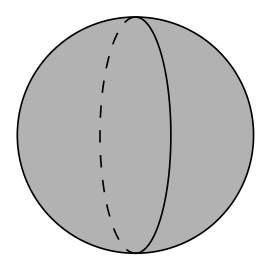
\includegraphics[width=0.10\textwidth]{p238_d1.png}\quad=\quad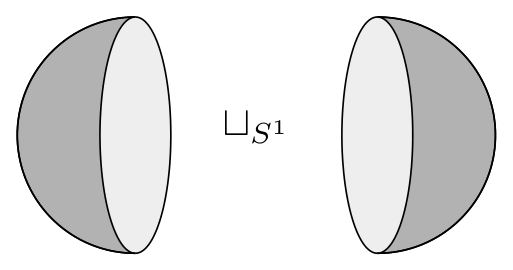
\includegraphics[width=0.22\textwidth]{p238_d2.png}
\end{equation}
（原文此处为示意图：$S^2$ 由两个半球沿 $S^1$ 粘合而成，右端标有 $\sqcup_{S^1}$），我们看到
\begin{equation}\tag{13.101}
\cZ(S^2)=\End\bigl(1_{\cZ(S^1)}\bigr),
\end{equation}
其中 $1_{\cZ(S^1)}$ 是平凡面缺陷。
% [Tutor Note: (13.100) 的图形在原书中为手绘示意（p.~237），此处保留原图。其含义是 $S^2$ 是 $S^1$ 上的“两个圆盘”的粘合，对应把线算子($S^2$) 写成面算子($S^1$) 的自同态；这正是 (13.101) 的内容。]

现在我们可以陈述：局部 Langlands 对应把 $G(K)$ 的光滑表示与 $\Loc_{G^\vee}(K)$ 联系起来/沿其谱分解。下面是一个具体的相应结果。

\begin{srcthm}{13 (Harris–Taylor, Henniart)}
对 $K$ 为局部域，$\mathrm{GL}_n(K)$ 的不可约光滑表示与 $K$ 上秩 $n$ 的 Galois 表示的同构类 $\Loc_{\mathrm{GL}_n}/\!\sim$ 双射。
\end{srcthm}
这是在说 $\Loc_{\mathrm{GL}_n}/\!\sim$ 在扮演某种 $\mathrm{GL}_n(K)$ 的 Pontrjagin 对偶的角色。但更一般的群呢？对一般群，人们已经（先由实验、现在已正式地）发现，$G(K)$ 的不可约表示映到 $\Loc_{G^\vee}$。即，这是自守到谱的方向：我们可以给一个不可约表示附上 Langlands 参数。
% [Tutor Note: 定理 13 中的“秩 $n$ Galois 表示”应理解为“$n$ 维 Galois 表示”（rank 指 $\mathrm{GL}_n$ 标准表示的维数，而非概形的秩）；且 $\Loc_{\mathrm{GL}_n}$ 此处指 $\Gal(K)$ 到 $\mathrm{GL}_n$ 的连续半单表示（带适当分歧条件）的栈，$\sim$ 表示同构。]

想法是：你应当能够给 $G(K)$ 的表示附上 Galois 表示，但这个映射不是一一的。这是在函数域设定中由 V.~Lafforgue–Genestier、在数域设定中由 Fargues–Scholze 给出的定理。这个映射的纤维称为 $L$-包。这些是 $L$-不可区分的表示，即 $L$-函数无法区分的表示。所以这不是一一对应，但这些包很小。

为什么我们有这种含糊性？其实我们应该在 $\Loc_{G^\vee}$ 上附一个层：一侧是 $G(K)$ 的表示，另一侧是 $\Loc_{G^\vee}$ 上某类层范畴。但 $\Loc_{G^\vee}$ 是栈，因为局部系统有自同构。所以即使一个层支撑在单个表示 $\rho:\Gal\to G^\vee$ 上，还有更多数据：$\Aut(\rho)$，即 $\rho$ 的中心化子，必须作用。于是我们得到
\begin{equation}\tag{13.102}
\Shv(\mathrm{pt}/Z(\rho))=\Rep(Z(\rho)).
\end{equation}
精细版本应说：$L$-包应构成这个中心化子 $Z(\rho)$ 的表示的一个子集，且这些表示在单位分支上平凡。即它是 $\pi_0(Z(\rho))$ 的表示。这告诉我们为什么应该期待这些包：我们先前把东西想得太过集合论了。

从这个图像我们得到一个全子范畴：
\begin{equation}\tag{13.103}
\Rep(G(K))\hookrightarrow \mathrm{Coh}(\Loc_{G^\vee}).
\end{equation}
这是局部 Langlands 对应的更精细版本。它在 $\mathrm{GL}_n$ 情形于 [BZCHN21] 中被证明。
% [Tutor Note: (13.102) 的 $\Shv(\mathrm{pt}/Z(\rho))$ 按定义就是 $Z(\rho)$-表示；之所以只剩下中心化子，是因为在栈上取点 $\mathrm{pt}\to\Loc$ 的纤维积要模掉稳定化子作用。这里 $Z(\rho)$ 可取为 $\rho$ 的 $\Gal$-中心化子（若 $\rho$ 不可约），其 $\pi_0$ 部分给出 $L$-包，连通部分给出无穷小特征。]

\begin{srcrem}{98}
这终于看起来像几何 Langlands 对应了。我们说局部域类似二维流形，而在几何 Langlands 中，谱侧是二维流形 $\Loc_{G^\vee}$ 上的某类凝聚层。但自守侧还不完全一样。
\end{srcrem}

如果我们看 $K=\C(\!(t)\!)$，那么这是一维流形的类比。所以我们该做高一层的事情，即我们在做局部几何 Langlands。于是我们考虑圈群
\begin{equation}\tag{13.104}
LG=G(K),
\end{equation}
并且不考察普通表示，而考察 $G(K)$-范畴。例如
\begin{equation}\tag{13.105}
G(K)\ \curvearrowright\ \Shv(G(K)/H)
\end{equation}
对任何子群 $H$。$LG=G(K)$-范畴的 2-范畴就是 TFT 附给一个圆周的东西：
\begin{equation}\tag{13.106}
\cA_G(S^1)=\Rep_{\mathbf{Cat}}(G(K)).
\end{equation}
于是我们可以把局部几何 Langlands 表述为：2-范畴 $\cA_G(S^1)$ 与 $\Loc_{G^\vee}(D^\times)$ 上的拟凝聚范畴层等同。如果我们改在 $\F_q(\!(t)\!)$ 上做这件事，那么它带有这个 Frobenius 作用；当我们取迹去范畴化时，就得到 $\F_q(\!(t)\!)$ 的局部 Langlands。

由此得到的局部 Langlands 版本实际上比我们上面表述的更好：我们得到等价而非全子范畴。我们先前对自守侧该放什么有点太天真了。有一个自然更大的范畴可供选择，它会与 $\mathrm{Coh}(\Loc_{G^\vee})$ 精确匹配。即 $\Rep(G(K))$ 太小了。下面的例子说明了这一点。

\begin{srcex}{93}
设 $G=T$。与其看所有表示，我们可以看非分歧表示。这只是一个 $T(K)$ 的表示，只不过现在我们取 $T(\cO)$ 的双陪集；但这是交换的（所以双陪集等同于单陪集），于是我们在考虑
\begin{equation}\tag{13.107}
\Gr_T=T(K)/T(\cO)\simeq\Lambda,
\end{equation}
其中 $\Lambda$ 是 $T$ 的特征格。于是
\begin{equation}\tag{13.108}
\Lambda\text{-}\mathbf{mod}\simeq\QC(T^\vee).
\end{equation}
\end{srcex}
% [Tutor Note: (13.107) 中仿射 Grassmann 簇 $T(K)/T(\cO)$ 的同构 $\simeq\Lambda$ 需固定一个均匀化子 $t$；作为格它是 $\Lambda$（余特征格，cocharacter lattice），而非特征格。原文称 $\Lambda$ 为 “character lattice”，此处照译但请注意：$T(K)/T(\cO)$ 自然地是余特征格。这一字之差会影响后续 $\Lambda$-mod 与 $\QC(T^\vee)$ 的对应方向。]
% [Tutor Note: (13.108) 中 $T^\vee$ 是环面，$\QC(T^\vee)$ 即 $\Lambda$-分次向量空间（取 $\Lambda$ 为 $T^\vee$ 的特征格时）。若按原文把 $\Lambda$ 当特征格，则 $\QC(T^\vee)$ 应是 $\Lambda^\vee=\Lambda$ 的分次，二者在环面情形恰好一致，故不影响结论。]

这看起来很好，但实际上这还不是全部。考虑非分歧局部系统：$\Loc^{\mathrm{unram}}_{T^\vee}$，即通过 Frobenius 分解的局部系统。于是其中之一由 Frobenius 在对偶群中的像，即 $T^\vee$ 的一个元素确定。但作为栈，它仍有自同构：
\begin{equation}\tag{13.109}
\Loc^{\mathrm{unram}}_{T^\vee}=T^\vee/T^\vee=T^\vee\times\mathrm{pt}/T^\vee.
\end{equation}
但当我们看它上面的层时，我们得到一个全子范畴：
\begin{equation}\tag{13.110}
\Lambda\text{-}\mathbf{mod}\simeq\QC(T^\vee)\hookrightarrow\QC(\Loc^{\mathrm{unram}}_{T^\vee}).
\end{equation}
即，我们先前只得到全子范畴（而非等价），是因为我们忽略了稳定化子。所以为了得到等价，我们需要这个额外因子：
\begin{equation}\tag{13.111}
\begin{array}{ccc}
\Lambda\text{-}\mathbf{mod} & \simeq & \QC(T^\vee)\\[4pt]
\downarrow & & \downarrow\\[4pt]
\Lambda\text{-}\mathbf{mod}\otimes\Rep(T) & \simeq & \QC\left(\Loc^{\mathrm{unram}}_{T^\vee}=\frac{T^\vee}{T^\vee}\right)
\end{array}
\end{equation}
% [Tutor Note: (13.111) 左下角的 $\Lambda\text{-}\mathbf{mod}\otimes\Rep(T)$ 中，$\Rep(T)$ 疑为 $\Rep(T^\vee)$ 之笔误：同一图右端是对偶环面的商栈 $T^\vee/T^\vee$，而 (13.112) 又把 $\Rep(T^\vee)$ 等同于 $\QC(\mathrm{pt}/T^\vee)$，所以“稳定化子修正”张量进来的应是对偶环面的表示范畴。原文照印 $\Rep(T)$，此处照译并标明。[译者按（无外部依据）]]
我们可以把这看作去范畴化的一次失败。当我们去范畴化时，对
\begin{equation}\tag{13.112}
\Rep(T^\vee)=\QC(\mathrm{pt}/T^\vee)
\end{equation}
有竖直/朴素的去范畴化和水平/聪明的去范畴化。竖直/朴素版本把这个范畴的 $\dim$ 当作普通范畴来取，得到
\begin{equation}\tag{13.113}
\dim\bigl(\Rep(T^\vee)\bigr)=\bigl(|\Rep(T^\vee)|,\bullet\bigr)=\cO(T^\vee).
\end{equation}
现在我们可以过渡到它上面的模：
\begin{equation}\tag{13.114}
\cO(T^\vee)\text{-}\mathbf{mod}=\QC(T^\vee).
\end{equation}
这是竖直/朴素的迹。

另一方面，我们可以取水平/聪明的版本，即把 $\Rep(T^\vee)$ 当作 $\otimes$-范畴来取 $\dim$；这更像代数的 Hochschild 同调，即最终会得到一个范畴。几何上，我们可以通过把 $\QC$ 与 $\dim$ 交换来计算它，即取 $\mathrm{pt}/T^\vee$ 的环路空间：
\begin{equation}\tag{13.115}
\QC\bigl(T^\vee/T^\vee=\mathcal{L}(\mathrm{pt}/T^\vee)\bigr).
\end{equation}
这是水平/聪明的迹。

注意这些并不一致：（竖直迹上的模）是水平迹的子范畴：
\begin{equation}\tag{13.116}
\QC(T^\vee)\hookrightarrow\QC(T^\vee/T^\vee).
\end{equation}
所以如果我们从几何 Langlands 出发，表述局部几何 Langlands，遵循我们一直遵循的同样规则，那么我们会试着去范畴化以弄清局部 Langlands 对应是什么。但我们可以做这两种迹。结论是：水平迹给你更好的东西。这已经出现在 V.~Lafforgue 的工作中，它引出了 excursion 算子的概念。这与先前的评论是同一回事：
\begin{equation}\tag{13.117}
\cO\left(\frac{G^\vee}{G^\vee}\right)\text{-}\mathbf{mod}\neq \QC\left(\frac{G^\vee}{G^\vee}\right).
\end{equation}
这个想法在 [AGK$^+$20b, AGK$^+$20a, AGK$^+$21] 中被精确化。
% [Tutor Note: (13.111) 的 2×2 图中第二行左端 $\Lambda$-mod$\otimes\Rep(T)$ 是把“稳定化子修正”张量进来；右端 $\QC(T^\vee/T^\vee)$ 正是水平迹（环路空间），它与 $\QC(T^\vee)$（竖直迹）的差别就是 (13.116) 的嵌入。(13.113) 中 $(\cdot,\bullet)$ 表示分次环（奇偶/度数），而 $\cO(T^\vee)$ 只看平凡分次，故竖直迹丢失了度数信息。]
% [Tutor Note: (13.117) 的不等号是本章最要紧的一句：$\cO(G^\vee/G^\vee)$-mod 是“朴素迹”，而 $\QC(G^\vee/G^\vee)$（即水平迹）才与自守侧匹配。这正是 V.~Lafforgue 的 excursion 算子与 AGK 的“谱分解”技术的关键差别，也是 (13.118) 要改用 $\IndCoh_{\mathrm{Nilp}}$ 的原因。]

\subsection{完整/范畴化局部 Langlands}\label{sec:13-6-4}

让我们回到算术设定（即 $K=\F_p(\!(t)\!)$、$\Q_p$ 等）。那么 $B$-侧是类似 $\QC(\Loc_{G^\vee})$ 的东西。然后我们希望它等价于某个包含 $\Rep(G(K))$ 作为全子范畴的范畴。答案是（拓扑）$\Bun_G$ 上的层，于是陈述的形状是\footnote{回忆 $\QC$ 其实应是 $\IndCoh_{\mathrm{Nilp}}$。}：
\begin{equation}\tag{13.118}
\Shv(\Bun_G)\simeq\QC(\Loc_{G^\vee}).
\end{equation}
所以我们只需弄清 $\Bun_G$ 是什么。我们知道
\begin{equation}\tag{13.119}
\Rep(G(K))=\Shv(\mathrm{pt}/G(K)),
\end{equation}
即它是某个空间中平凡丛轨迹上的层。所以会有一个更大的空间叫 $\Bun_G$，如果只看平凡丛，它的自同构是 $G(K)$。于是 $G(K)$ 的表示会作为生活在平凡丛轨迹上的层出现。但我们缺了这个空间的其余部分，而这就是几何 Langlands 观点所提议的。

这个 $\Bun_G$ 有两个版本。在函数域上更容易说：
\begin{equation}\tag{13.120}
\Bun_G=G(K)/_F G(K),
\end{equation}
其中 $/_F$ 表示模掉 Frobenius 扭共轭，即模掉作用
\begin{equation}\tag{13.121}
h*g=hgFh^{-1}.
\end{equation}
这来自顺着我们的鼻子走：如果我们想 $\Bun_G(D^\times)=\mathrm{pt}/G(K)$，然后求 Frobenius 的不动点。同构类的集合
\begin{equation}\tag{13.122}
G(K)/_FG(K)
\end{equation}
由所谓的 Kottwitz $G$-同晶（isocrystal）构成。

这预期大致等价于 Fargues–Scholze 的某个版本。他们研究某条特定曲线——称为 Fargues–Fontaine 曲线——上 $\Bun_G$ 的层。所以这真的是把“局部 Langlands 应该是某条特定曲线上的几何 Langlands”这个想法放在心上。即局部域 $K$ 应对应于某条曲线。在 $K=\Q_p$ 的情形，这条曲线大致是
\begin{equation}\tag{13.123}
\Spec\Q_p/\Z,
\end{equation}
其中 $\Z$ 通过 Frobenius 作用。我们可以把它想成某种模 Frobenius 的穿孔圆盘。要正确地说出这件事，你需要整套完美胚（perfectoid）机器。
% [Tutor Note: (13.118) 的脚注不可略过：光滑/有限型假设下 $\QC$ 与 $\IndCoh$ 的差别在 $\Bun_G$ 这类非有限型、非光滑对象上是本质的；正确陈述用 $\IndCoh_{\mathrm{Nilp}}(\Loc_{G^\vee})$。(13.120) 的 Kottwitz 同晶集合并不能直接给出 $\Bun_G$ 的几何结构，取 $G(K)/_FG(K)$ 作为“空间”只是对同构类的粗描述。]
% [Tutor Note: (13.121) 中 $F$ 是 Frobenius 自同构，$h*g=hgFh^{-1}$ 中的 $gF$ 表示 $\sigma$-线性作用；把它读作“$h g \sigma(h)^{-1}$”更不会出错。$\Bun_G=G(K)/_FG(K)$ 只对函数域（或完美胚意义下的 $\Q_p$）有意义，见 Fargues–Fontaine 曲线。]

\begin{flushright}\small 第 33 讲；2021 年 6 月 24 日\end{flushright}

\chapter{导出代数几何}\label{ch:14}

\begin{keytakeaways}
本章解释为什么局部算子比交换代数“多一层”：一个 $n$ 维拓扑场论中，局部算子空间 $A=\cZ(S^{n-1})$ 带有 $\mathbb{E}_n$-代数结构（小 $n$ 圆盘算子代数），而 Dunn–Lurie 可加性 $\mathbb{E}_k+\mathbb{E}_\ell=\mathbb{E}_{k+\ell}$ 解释了它的来源。取上同调后 $\mathbb{E}_n$ 退化为 $\PP_n$-代数：$n=1$ 是普通 Poisson 代数，$n=2$ 是 Gerstenhaber 代数，$n\ge3$ 是（分次）Poisson 代数。于是非交换的 $\mathbb{E}_n$-代数应看成 $\PP_n$-代数的量子化，其“经典极限”是移位辛（shifted symplectic）簇；B-模型的真空模空间正是 $T^*[1]X$，它上面的形变量子化给出可观测量的代数 $\mathrm{HH}^*$，而几何量子化给出态范畴 $\QC(X)$。最后讨论切向结构（定向 vs 标架）如何迫使我们在 $\mathrm{HH}_*$ 与 $\mathrm{HH}^*$ 之间选一个等同，即选一个体积形式。
\end{keytakeaways}

\section{拓扑场论与 $\mathbb{E}_n$-代数}\label{sec:14-1}

\begin{sectionkey}
本节从拓扑扭转出发，说明 TFT 中“局部算子”为什么天然带有 $\mathbb{E}_n$-代数结构：它来自把 $k$ 个小圆盘嵌入大圆盘的构型空间的作用。核心是把“结合积”升级为“构型空间参数化的多重复积”，这也是 $\mathbb{E}_n$ 定义的几何来源。
\end{sectionkey}

对物理学家来说，拓扑场论大致有两个来源。第一个来源是那些我们可以直接写下来、明显是拓扑的理论，例如有限群例子和 Chern–Simons 理论。但大多数有趣的拓扑理论不是这样产生的。第二个来源是由拓扑扭转产生的理论。

\term{拓扑扭转}{topological twisting}的想法如下。从一个“诚实的”（欧氏的）量子场论出发。它是定义在 Riemann 流形范畴上的某种函子。然后某些特殊的量子场论具有超对称（SUSY）。这意味着我们有某个有趣的超李代数的作用。有特定的算子 $Q$，称为 BRST 算子，它们是我们的态空间上的奇、次数 1 的自同态。于是我们有一个满足 $Q^2=0$ 的算子，因此可以过渡到上同调。

大多数 QFT 不是 SUSY 的，大多数 SUSY 理论也不是拓扑的。但人们常常发现理论具有这样的结构：所谓的应力张量 $T$ 是 $Q$-恰当的。注意这是一种\emph{结构}而不是\emph{性质}。应力张量是（物理中）描述对几何/度规变化的响应的对象。所以如果这种对几何变化的依赖是 $Q$-恰当的，那么在上同调层面，理论就不依赖于几何。实际上，应力张量控制我们的场论 $Z$ 在 Riemann 流形模空间上的变化。例如，从 $S^1\sqcup S^1$ 到 $S^1$ 的 Riemann 配边构成整个空间。于是 $Z$ 把它送到一族映射 $Z(S^2)^{\otimes2}\to Z(S^1)$。它是 $Q$-恰当的这一事实意味着，在上同调层面，这种对几何的依赖是局部常值的。

% [Tutor Note: 上一段末尾的 $Z(S^{2})^{\otimes 2}\to Z(S^{1})$ 疑为原书笔误：$\Sigma$
% 是从 $S^{1}\sqcup S^{1}$ 到 $S^{1}$ 的配边，故 $Z(\Sigma)$ 应是
% $\Hom\bigl(Z(S^{1})^{\otimes 2},Z(S^{1})\bigr)$ 中的族，紧接的 (14.1)(14.2) 也正写作
% $Z(S^{1})^{\otimes 2}$；译文照印本保留 $S^{2}$，不改动数学。
% [译者按（无外部依据）：由同段 (14.1) 的内部一致性判定，未找到外部依据。]]
当我们有一个 TFT $Z$ 时，如果 $\Sigma$ 是从 $S^1\sqcup S^1$ 到 $S^1$ 的配边，即带三个穿孔的曲面，那么我们预期 $Z(\Sigma)$ 是所有这类配边的模空间上的局部常值函数，取值于
\begin{equation}\tag{14.1}
\Hom\left(Z(S^1)^{\otimes2},Z(S^1)\right).
\end{equation}
在链的层面，我们可以把它改写为
\begin{equation}\tag{14.2}
Z\in\Hom\left(Z(S^1)^{\otimes2},Z(S^1)\right)\otimes C^*(M).
\end{equation}
或者等价地，它定义了一个映射
\begin{equation}\tag{14.3}
C_*(M)\otimes Z(M_{in})\to Z(M_{out}).
\end{equation}
% [Tutor Note: (14.1)--(14.3) 是同一件事的三种说法：$Z(\Sigma)$ 在配边模空间上局部
% 常值，即 $Z$ 给出该模空间上的局部常值链复形（局部系统），故 (14.2) 把它写成
% $\Hom(\cdots)\otimes C^{*}(M)$；再用张量–$\Hom$ 伴随把 $C^{*}(M)$ 搬到另一侧，
% 就是 (14.3) 的 $C_{*}(M)\otimes Z(M_{\mathrm{in}})\to Z(M_{\mathrm{out}})$。原书
% (14.2) 用上标 $C^{*}$、(14.3) 用下标 $C_{*}$，互为对偶（$C^{*}\cong(C_{*})^{\vee}$），经张量–$\Hom$ 伴随等同；译文照原文未统一写法。
% [译者按（无外部依据）：由 (14.1)--(14.4) 的内部一致性判定。]]

另一种写法如下。设 $|M|$ 为 Riemann 配边的模空间。这是空间 $M$ 底层的同伦型/anima/$\infty$-群胚。那么这等同于一个映射
\begin{equation}\tag{14.4}
|M|\to\Hom(Z(M_{in}),Z(M_{out})).
\end{equation}
在范畴层面我们得更小心“局部常值”是什么意思，即我们需要区分 de Rham 与 Betti 设定。我们或许会看从 $M$ 的 de Rham 空间到“运算”的映射，这可以称为 de Rham 场论。Betti 版本则考虑从 $|M|$ 到“运算”的映射。在函数/向量空间的层面这没有区别，但局部常值层有两个版本：一个平坦联络并不会自动给你平行移动。

\subsection{局部算子上的 $\mathbb{E}_n$-代数结构}\label{sec:14-1-1}

我们假定处在这个局部常值/Betti 的情形。我们想关注局部算子上得到的结构。回忆我们有过这样的想法：局部算子空间
\begin{equation*}
A=\cZ(S^{n-1})
\end{equation*}
作用在 $\cZ(M^{n-1})$ 上，对任何 $(n-1)$-流形 $M^{n-1}$。现在我们将在导出的设定中重新审视这一点。当我们想复合局部算子时，我们画的图如下：
\diagram[0.14\textwidth]{p243_d1.png}
它给出乘法：
\begin{equation}\tag{14.5}
A^{\otimes2}\to A.
\end{equation}
对 $n>1$，球可以互相移动，于是我们得到交换的乘法（在非导出层面）。更好的说法是
\begin{equation}\tag{14.6}
H_0\bigl(\mathrm{Conf}_2(D^n)\bigr)=\Z,
\end{equation}
即 $D^n$ 中两点的构型空间是连通的。一般地，场论给我们一个映射
\begin{equation}\tag{14.7}
\mathrm{Conf}_k(D^n)\to\Hom\left(A^{\otimes k},A\right).
\end{equation}
当我们过渡到导出设定，这就是所谓的 $\mathbb{E}_n$-代数的定义。即 $A$ 是小 $n$ 圆盘\term{操作子}{operad}上的代数。这告诉我们有一个映射
\begin{equation}\tag{14.8}
C_*\bigl(\mathrm{Conf}_k(D^n)\bigr)\to\Hom\left(A^{\otimes k},A\right).
\end{equation}
拓扑上，我们可以简单地说有一个映射
\begin{equation}\tag{14.9}
\left|\mathrm{Conf}_k(D^n)\right|\to\Hom\left(A^{\otimes k},A\right).
\end{equation}
于是就给出了任何对称幺半高阶范畴中 $\mathbb{E}_n$-代数的概念。
% [Tutor Note: (14.5)--(14.9) 的关键是“构型空间参数化运算”：$n=1$ 时 $\mathrm{Conf}_k(D^1)$ 不连通（有 $k!$ 个分量），给出结合的乘法和置换；$n>1$ 时连通，给出交换乘法。所谓“导出”就是把 $\mathrm{Conf}_k(D^n)$ 换成它的链复形/同伦型，从而把“只在同伦意义下交换”精化为 $\mathbb{E}_n$ 结构。切勿把 (14.7) 读成“每个构型给一个映射”，它在导出层面是一个 $\mathrm{Conf}_k$ 上的局部系统。]
% [Tutor Note: 上文“操作子”是 operad 的译名（May 意义下的“小 $n$ 圆盘”operad：
% 每个 $k$ 给构型空间 $\mathrm{Conf}_k(D^n)$，用其链复形记录 $k$ 元运算及其替换），
% 与泛函分析里的 operator algebra 无关。第 11、15 章在同样语境下直接写英文
% operad，本仓库资料卡作“操作子”，三种写法尚未统一，读时按 operad 理解即可。
% [来源：本仓库资料卡 functoriality/concept/operad]]

\begin{srcrem}{99}
我们可以在任何对称幺半高阶范畴中定义 $\mathbb{E}_n$-代数的概念，但有时该范畴被假定为链复形范畴，这时人们就径称 $\mathbb{E}_n$-代数。
\end{srcrem}

\begin{srcex}{94}
在（普通/离散/非导出）$\Vect$ 中的 $\mathbb{E}_n$-代数，对 $n=1$ 就是结合代数，对 $n>1$ 就是交换代数。
\end{srcex}

\begin{srcex}{95}
在（普通/离散/非导出）$\mathrm{Cat}$ 中的 $\mathbb{E}_n$-代数：$n=1$ 是幺半范畴，$n=2$ 是编织幺半范畴，$n>2$ 是对称幺半范畴。
\end{srcex}

\subsection{$\mathbb{E}_n$-代数的来源}\label{sec:14-1-2}

$\mathbb{E}_n$-代数的“原初”例子如下。设 $X$ 是带基点的拓扑空间。考虑 $X$ 中的 $n$ 重基点环路空间 $\Omega^nX$。我们应该把它想成
\begin{equation}\tag{14.10}
\mathrm{Map}\left((\R^n,\R^n\setminus D^n),(X,*)\right)=\mathrm{Map}\left(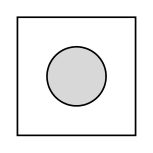
\includegraphics[width=0.045\textwidth]{p244_d1.png},(X,*)\right).
\end{equation}
即从 $\R^n$ 到 $X$ 的映射空间，使得 $D^n\subset\R^n$ 的补集映到基点。通过把多个圆盘放进一个更大的圆盘，我们得到复合映射。于是我们得到一个映射
\begin{equation}\tag{14.11}
\left|\mathrm{Conf}_kD^n\right|\times(\Omega^nX)^k\to\Omega^nX.
\end{equation}
即 $\Omega^nX$ 是空间范畴中的 $\mathbb{E}_n$-代数。这是“对 $n>1$，$\pi_n(X)$ 交换”这一事实的花哨版本：
\begin{equation}\tag{14.12}
\pi_0(\Omega^nX)=\pi_n(X).
\end{equation}

\begin{srcthm}{14（识别定理）}
若 $Y$ 是足够连通的空间，则把 $Y$ 与某个 $n$ 重环路空间等同起来，$Y\overset{\sim}{\longrightarrow}\Omega^nX$，对应于 $Y$ 上的 $\mathbb{E}_n$-结构。
\end{srcthm}

\subsection{可加性}\label{sec:14-1-3}

关于 $\mathbb{E}_n$-代数最重要的想法是它们满足某个版本的可加性。我们将使用的版本称为 Dunn–Lurie 可加性，它说
\begin{equation}\tag{14.13}
\mathbb{E}_k+\mathbb{E}_\ell=\mathbb{E}_{k+\ell}.
\end{equation}
我们先前见过它的一个基本版本：如果我们有两个相容的结合运算，那么它们被迫相等且交换。所以这在更大的一般性下成立：$\mathbb{E}_\ell$-代数中的 $\mathbb{E}_k$-代数是一个 $\mathbb{E}_{k+\ell}$-代数。理解这一点的一种方式是：它告诉我们 $\mathbb{E}_n$ 是什么意思——它是装备了 $n$ 个相容结合积的对象。

\subsection{范畴表现}\label{sec:14-1-4}

$\mathbb{E}_n$-代数可以看成 $n$-截断的 $n$-范畴。结果这实际上是一个等价。

$\mathbb{E}_1$-代数是结合代数的导出版本。即它是幺半群，也就是带单个对象 $(\cC,*)$ 的范畴。对 $(\cC,*)$ 我们可以附上代数 $\End(*)$。反方向上，给定代数 $A$，我们可以附上带单个对象 $*$、其自同态由 $\End(*)=A$ 给出的范畴 $BA$。这就是 $\mathbb{E}_1$-代数与带单个对象的范畴之间的对应：
\begin{align}
\End(*)&\leftarrow(\cC,*) \tag{14.14}\\
A&\mapsto BA. \tag{14.15}
\end{align}
类似地，我们可以考虑带一个对象 $*$ 和一个 1-态射 $1_*$ 的 2-范畴。那么我们可以把它送到结合代数 $A=\End(1_*)$。但这个单态射 $1_*$ 是 1-态射复合的单位。$1_*$ 与自身的复合给出 $A$ 上新的结合结构，即由可加性，$A$ 事实上是 $\mathbb{E}_2$-代数。于是这个 2-截断 2-范畴给了我们一个 $\mathbb{E}_2$-代数。

我们也可以做介于两者之间的事情。给定 1-截断的 2-范畴 $(\cC,*)$（即带单个对象的 2-范畴），我们可以考虑 $A=\End(*)$，它是幺半（$\mathbb{E}_1$）范畴。结果 1-截断 2-范畴等价于 $\mathbb{E}_1$-范畴。

想法是：如果我们有一个 $n$-范畴，并且它是 $n$-截断的（即一路下去只有一个 $n$-态射），那么我们就会发现
\begin{equation}\tag{14.16}
A=\End\left(1_{1\cdots1}\right)
\end{equation}
有 $n$ 个相容乘法。所以 $\mathbb{E}_n$ 中的 $n$ 与 $n$-范畴中的 $n$ 是同一个 $n$。这总结在高阶范畴的周期表中，即表 14.1。
% [Tutor Note: (14.16) 中的 $1_{1\cdots1}$ 是“一路复合到底”的单个 $n$-态射的记号，原书用嵌套下标表示（$1_{1_{\cdot_{\cdot}}}$）；这里按行文线性化为 $1_{1\cdots1}$，含义不变：这个自同态代数带有 $n$ 个相互相容的乘法。]

\begin{table}[htbp]
\centering
\caption{高阶范畴的周期表。BTC 代表编织张量范畴。（原文 p.~244，Table 14.1）}
\label{tab:14-1}
\small
\begin{tabular}{c|ccc}
\toprule
\multicolumn{1}{c}{} & \multicolumn{3}{c}{cat\#}\\
\cmidrule(lr){2-4}
truncated\# & 1 & 2 & 3\\
\midrule
1 & $\mathbb{E}_1$-algebra & $\mathbb{E}_1$-category & $\mathbb{E}_1$ 2-category\\
2 & & $\mathbb{E}_2$-algebra & $\mathbb{E}_2$-category (BTC)\\
3 & & & $\mathbb{E}_3$-algebra\\
\bottomrule
\end{tabular}
\end{table}

与其看这些带单个对象的小截断范畴，我们可以谈论由单个对象\emph{生成}的范畴。我们希望有结合（$\mathbb{E}_1$）代数与带点（$\mathbb{E}_0$）范畴之间的字典。对 $(\cC,*)$ 为 $\mathbb{E}_0$-范畴，我们可以附上结合代数 $\End(*)$。反方向上，给定结合代数 $A$，我们可以把它送到范畴 $A\text{-}\mathbf{mod}$，并带一个被指定的对象 $A\in A\text{-}\mathbf{mod}$。函子 $\End(*_{(-)})$ 与 $(-)\text{-}\mathbf{mod}$ 互为伴随。这是把上述字典换一种写法（$BA$ 可以从 $A\text{-}\mathbf{mod}$ 恢复），但现在范畴有余极限之类的东西，于是表示论中感兴趣的范畴就纳入这个框架。

\begin{srcex}{96}
设 $\cC$ 是幺半（$\mathbb{E}_1$）范畴。那么我们有一个结合代数
\begin{equation}\tag{14.17}
\End(1_{\cC})=A.
\end{equation}
但这实际上是 $\mathbb{E}_2$-代数，因为 $1_{\cC}$ 是单位。并且我们有嵌入
\begin{equation}\tag{14.18}
A\text{-}\mathbf{mod}\hookrightarrow\cC.
\end{equation}
如果 $A$ 是 $\mathbb{E}_2$-代数，那么 $A\text{-}\mathbf{mod}$ 事实上是幺半的。即取 $-\text{-}\mathbf{mod}$ 会把你降一个 $\mathbb{E}_n$ 层级。
\end{srcex}

\begin{srcex}{97}
如果 $A$ 是 $\mathbb{E}_n$-代数，那么 $A\text{-}\mathbf{mod}$ 是 $\mathbb{E}_{n-1}$-范畴。于是我们可以取这个范畴并寻找它的模：$A\text{-}\mathbf{mod}\text{-}\mathbf{mod}$，它是 $\mathbb{E}_{n-2}$-2-范畴。我们可以把这个过程继续 $n$ 次，得到一个 $n$-范畴：
\begin{equation}\tag{14.19}
A\text{-}\mathbf{mod}\cdots\text{-}\mathbf{mod}=A\text{-}\mathbf{mod}^n.
\end{equation}
\end{srcex}

\begin{srcrem}{100}
这都是说 $n$-范畴基本上只是 $\mathbb{E}_n$-代数的更花哨/更一般的版本。就像范畴是结合代数的花哨版本，只不过我们只有这种部分定义的乘法。
\end{srcrem}
% [Tutor Note: 表 14.1 在原文中是一张 4×4 的排版表（p.~244），图文件 \texttt{table14-1.png} 的裁剪把表后正文一并包含进来、不宜直接插图，故按本书规范（guide §3.3：能可靠重排则优先重排）用 booktabs 重排；内容与原文逐格一致。]
% 若确需用图像版，可改为：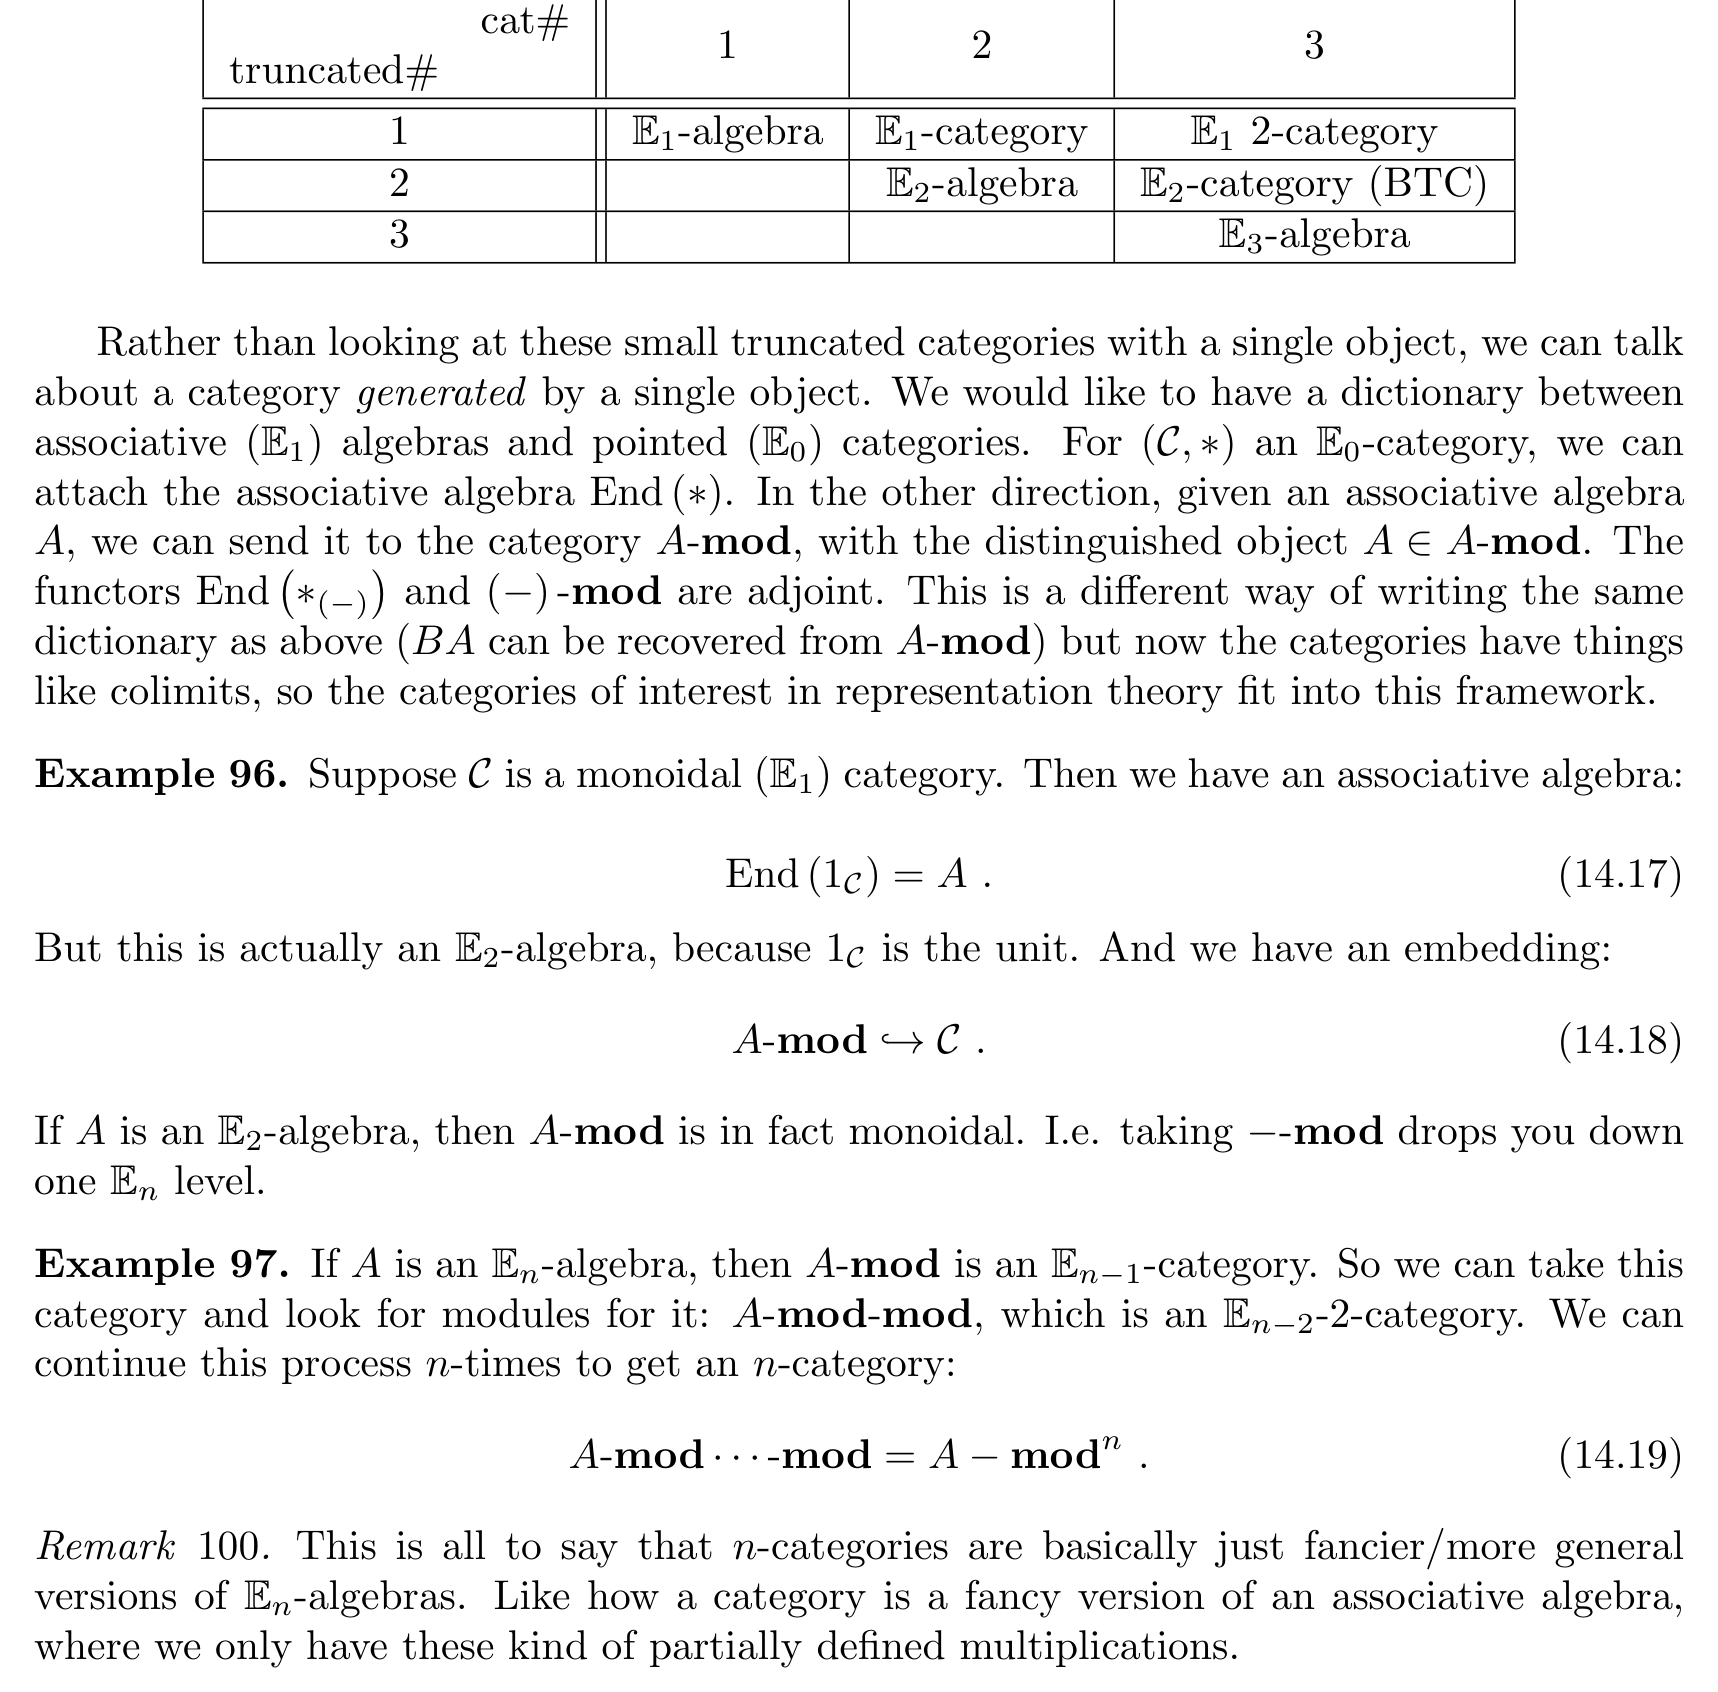
\includegraphics[trim=0 1332 0 0,clip,width=0.85\textwidth]{table14-1.png}（裁去表后正文）。

\section{Hochschild 上同调}\label{sec:14-2}

\begin{sectionkey}
本节说明结合代数 $A$ 的中心/Hochschild 上同调 $\mathrm{HH}^*(A)=\End_{A\text{-}\mathbf{mod}\text{-}A}(A)$ 天然是 $\mathbb{E}_2$-代数（Deligne 猜想，由 Dunn–Lurie 可加性推出），并在上同调层面退化为 Gerstenhaber 代数：一个次数 0 的交换乘法加上一个次数 $-1$ 的 Poisson 括号。HKR 定理把它具体化为外代数 $\wedge^\bullet T_M$ 上的 Schouten–Nijenhuis 括号。
\end{sectionkey}

对 $A$ 为结合代数，我们附上它的中心/Hochschild 上同调
\begin{equation}\tag{14.20}
Z(A)=\mathrm{HH}^*(A)=\End_{A\text{-}\mathbf{mod}\text{-}A}(A).
\end{equation}
Gerstenhaber 发现 Hochschild 上同调带有 Gerstenhaber 代数的额外结构。我们先讨论导出版本。

我们知道 $\mathrm{HH}^*(A)$ 是结合的，因为它是某个东西的 $\End$。但双模给出一个由张量积给出的函子
\begin{equation}\tag{14.21}
(-)\otimes_A B_A:\ A\text{-}\mathbf{mod}\to A\text{-}\mathbf{mod}.
\end{equation}
所以 $A$ 是单位双模，即这是 $A\text{-}\mathbf{mod}$ 的 Bernstein 中心，而这就贡献了第二个结合积。于是我们从“是 $\End$”得到一个结合乘法，但它在幺半范畴中是单位，于是我们得到第二个方向的乘法，即它是 $\mathbb{E}_2$-代数。这就是所谓的 Deligne 猜想，它说结合代数 $A$ 的 Hochschild 链复形自然地是 $\mathbb{E}_2$-代数。现在我们可以看出这是 Dunn–Lurie 可加性的平凡推论。
% [Tutor Note: Deligne 猜想（$\mathrm{HH}^{*}(A)$ 上自然的 $\mathbb{E}_2$ 结构）如今已是
% 定理，McClure--Smith 给出了证明。书中说它是可加性的“平凡推论”，指的是在
% $\mathbb{E}_n$ 框架就位后这一步变成形式论证，并不等于说猜想本身无需证明。
% [来源：McClure--Smith《A solution of Deligne's Hochschild cohomology conjecture》，Contemp. Math. 293 (2002)]]

于是对 $\cC$ 为范畴，说 $\cC$ 是 $A$-线性的（$A$ 为任意 $\mathbb{E}_2$-代数）是有意义的：我们只需一个 $\mathbb{E}_2$ 映射
\begin{equation}\tag{14.22}
A\to\End(\mathrm{id}_{\cC}).
\end{equation}
另一种说法是：我们可以取 $A$，考虑幺半范畴 $A\text{-}\mathbf{mod}$，然后可以要求 $A\text{-}\mathbf{mod}$ 作用在 $\cC$ 上。

回忆我们说过任何范畴 $\cC$ 都沿
\begin{equation}\tag{14.23}
\Spec Z(\cC)=\Spec\End(\mathrm{id}_{\cC})
\end{equation}
谱分解。但现在这是 $\mathbb{E}_2$-代数的 $\Spec$。下面我们聚焦于 Gerstenhaber 在上同调层面发现的更具体的结构。
% [Tutor Note: (14.20) 中把中心与 Hochschild 上同调等同，只在 $A$ 为光滑（或至少 $\mathrm{HH}^*$ 与 $\End_{A^e}(A)$ 一致）时成立；一般情形 $\End_{A^e}(A)$ 是导出中心，而 $Z(A)$ 只是 $\pi_0$。(14.21) 的 $B_A$ 指 $A$-双模。(14.23) 的 $\Spec$ 应取导出意义下的谱，这也是本章标题“导出代数几何”的由来。]

\subsection{Gerstenhaber 代数}\label{sec:14-2-1}

回忆作为（链复形中的）$\mathbb{E}_n$-代数意味着我们有作用
\begin{equation}\tag{14.24}
C_*\bigl(\mathrm{Conf}_k(\R^n)\bigr)\otimes A^{\otimes k}\to A.
\end{equation}
F.~Cohen 在上同调层面给出了解释，即我们取非导出版本。该结构是一个映射
\begin{equation}\tag{14.25}
H_*\bigl(\mathrm{Conf}_k(\R^n)\bigr)\to H^*(A)^{\otimes k}\to H^*(A).
\end{equation}
带有这种额外结构的分次向量空间称为 $\PP_n$-代数。即
\begin{equation}\tag{14.26}
\PP_n=H_*(\mathbb{E}_n).
\end{equation}
具体地说，$\PP_n$-代数 $B=H^*(A)$ 有一个次数 0 的交换乘法，而在次数 $1-n$ 处我们得到另一个运算，记作 $\{\,\}$。因为
\begin{equation}\tag{14.27}
\mathrm{Conf}_2(\R^n)\simeq S^{n-1},
\end{equation}
所以我们有两个类：
\begin{equation}\tag{14.28}
H_0(S^{n-1})\oplus H_{n-1}(S^{n-1}).
\end{equation}
定理是：次数 0 的分量是乘法，而次数 $n-1$ 的贡献是次数 $1-n$ 的 Poisson 括号 $\{\,\}$。Poisson 意味着它是（超）导子。

\begin{srcex}{98}
$\PP_1$-代数就是普通的 Poisson 代数。
\end{srcex}

\begin{srcex}{99}
$\PP_3$-代数等同于普通的 Poisson 代数，只不过底层向量空间是分次的，且括号的次数为 $-2$。
\end{srcex}

\begin{srcex}{100}
$\PP_2$-代数就是所谓的 Gerstenhaber 代数。即它带有一个次数 $-1$ 的 Poisson 括号。
\end{srcex}

于是定理是：$\mathrm{HH}^*(A)$ 带有自然的 $\PP_2$-结构。

\begin{srcex}{101}
Gerstenhaber 代数的主要例子是 Schouten–Nijenhuis 括号。考虑外代数 $\wedge^\bullet T_M$。有楔积，但此外还有括号 $\{\,\}=[\,,]_{SN}$，它由下述要求唯一确定：
\begin{equation}\tag{14.29}
T_M\otimes T_M\to T_M
\end{equation}
是通常的李括号，只不过现在次数为 $-1$。
\end{srcex}

\begin{srcthm}{15（Hochschild–Kostant–Rosenberg（HKR））}
\begin{equation}\tag{14.30}
\mathrm{HH}^*(C^\infty(M))\simeq\wedge^\bullet T_M=\mathrm{Sym}\,T[-1],
\end{equation}
其中 $\{\,,\}$ 对应于 $[\,]$。
\end{srcthm}
% [Tutor Note: 定理名的三位作者是 G. Hochschild、B. Kostant、A. Rosenberg。原书
% p.~246 印作 “Hochschild-Konstant-Rosenburg”；先前已把 “Rosenburg” 按通行拼写
% 改为 “Rosenberg”，此处再把 “Konstant” 改回 “Kostant”，与第 15 章的
% “Hochschild--Kostant--Rosenberg” 及文献一致。
% [来源：Hochschild--Kostant--Rosenberg《Differential forms on regular affine algebras》，Trans. Amer. Math. Soc. 102 (1962)]]

这在代数几何中也成立，即对 $X$ 为仿射簇、用 $\cO(M)$（而非 $C^\infty(M)$）。

然后 Deligne 问：这个括号能否提升为 $\mathbb{E}_2$-结构？这就是 Deligne 猜想。

\begin{srcex}{102}
考虑 $\mathbb{E}_3$-代数。交换（同伦意义下）的乘法来自 OPE，即点碰撞。括号来自把一个算子放在原点，而把另一个算子放在环绕原点的球面上。所以这其实只是说括号来自 $H_2(S^2)$ 中的基本类。
\end{srcex}
还有一种很酷的画法，用 Hopf 链环。想象取一个算子并让它绕一个圆移动，另一个算子也绕一个圆移动。这个环面表示 $\R^3$ 中两点构型空间的 $H_2$ 中的同一个类。

设 $\cZ$ 是 $n$ 维 TFT。结论是 $\cZ(S^{n-1})$ 是 $\mathbb{E}_n$-代数。具体地说，这意味着
\begin{equation}\tag{14.31}
H^*\bigl(\cZ(S^{n-1})\bigr)
\end{equation}
是（分次）Poisson 的。于是取 $\Spec$ 就得到 Poisson 簇 $\Spec H^*\bigl(\cZ(S^{n-1})\bigr)$，它常常实际上是辛的（即括号非退化）。

\begin{srcex}{103}
回忆 $\wedge^\bullet T_M=\mathrm{Sym}\,T_M[-1]$。那么我们有
\begin{equation}\tag{14.32}
T^*[1]M=\Spec(\wedge^\bullet T_M),
\end{equation}
它是奇 Poisson 簇，即带有次数 $-1$ 括号的簇。换句话说，HKR 说
\begin{equation}\tag{14.33}
\Spec\mathrm{HH}^*(M)=T^*[1]M.
\end{equation}
\end{srcex}
% [Tutor Note: (14.28)--(14.30) 的符号最易出错：$\mathrm{Conf}_2(\R^n)\simeq S^{n-1}$ 的定向决定了括号的符号（Koszul 符号）；$\wedge^\bullet T_M=\mathrm{Sym}\,T[-1]$ 中的 $[-1]$ 是“平移”，即把 $T_M$ 放在次数 1，于是 $\wedge^kT_M$ 落在次数 $k$，这与 $\mathrm{HH}^*$ 的度数一致。(14.33) 的 $\Spec$ 是导出 $\Spec$（取分次交换环的谱），所以得到的是 $1$-移位辛簇而非普通簇。]

事实上它是 1-移位辛流形。关于移位辛几何的更多内容见 [PTVV13, CPT$^+$17]。

实践中，我们从移位辛几何中只需要普通辛几何中我们需要的东西：函数带有 Poisson 括号。即，无论 $n$-移位辛流形是什么，其上的函数应当是 $\PP_n$ 的。而当我们这样表述时，就清楚了：移位辛流形就是为了被量子化，即从 $\PP_n$ 提升到 $\mathbb{E}_n$。
% [Tutor Note: “移位辛”（shifted symplectic）的移位量等于括号的次数：$n$-移位辛流形的函数环是 $\PP_n$（即括号次数 $1-n$）。(14.32) 的 $T^*[1]M$ 是 1-移位辛的，故其函数是 $\PP_2$（Gerstenhaber）；这正是 $\mathrm{HH}^*$ 的情形。若把它误当成普通辛流形（0-移位），括号次数会算错 1——这是本节最常见的指标错误。]

\section{量子化}\label{sec:14-3}

\begin{sectionkey}
本节把 $\mathbb{E}_n$ 与 $\PP_n$ 的关系总结为“量子化”：正如结合代数是 Poisson 代数的量子化，$\mathbb{E}_n$-代数是 $\PP_n$-代数的量子化。由此 TFT 的局部算子是“几乎交换”的，其“经典极限”是移位辛簇；要容纳它需要 $\mathbb{E}_n$-代数几何。最后用 B-模型说明 $X\hookrightarrow T^*[1]X$ 是拉格朗日嵌入，而定向理论需要在 $\mathrm{HH}_*$ 与 $\mathrm{HH}^*$ 之间选一个体积形式。
\end{sectionkey}

这引向对 $\mathbb{E}_n$-代数的另一种观点：它们是 $\PP_n$-代数的量子化。我们应把这看作“$\mathbb{E}_1$-代数是 $\PP_1$-代数的量子化”这一想法的类比，其含义如下。对 $A_\hbar$ 为结合代数，依赖于某个参数 $\hbar$，使得 $A_{\hbar=0}$ 是交换的，那么 $A_{\hbar=0}$ 获得一个 Poisson 括号：
\begin{equation}\tag{14.34}
\{a,b\}=\frac{ab-ba}{\hbar}\bmod\hbar.
\end{equation}
这是量子力学与经典力学相互作用的经典方式：经典力学中我们有普通 Poisson 括号，而如果我们有一个结合代数在某个参数值处变成交换的，那么自然得到一个 Poisson 括号。而 Poisson 括号告诉你把交换形变到结合的一阶数据。Poisson 是某种“结合在交换处的切空间”。

现在同类的故事推广到 $\mathbb{E}_n$。对 $A$ 为 $\mathbb{E}_n$-代数，其上同调 $H^*(A)$ 是交换的。然后它获得括号 $\{\,\}$ 而成为 $\PP_n$-代数。这个括号是成为交换的障碍。我们真正想说的是：对 $A$ 为 $\mathbb{E}_n$-代数，我们确实得到一个典范李括号。所以有某种正合列
\begin{equation}\tag{14.35}
\mathrm{Comm}\to\mathbb{E}_n\to\mathrm{Lie}[1-n].
\end{equation}
就像我们曾有
\begin{equation}\tag{14.36}
\mathrm{Comm}\ \xleftarrow{\ \ }\ \mathrm{Assoc}\ \xrightarrow{\ [\,]\ }\ \mathrm{Lie},
\qquad U:\ \mathrm{Lie}\to\mathrm{Assoc}.
\end{equation}
这件事的结论是：TFT 中的局部算子，对 $n>1$，是几乎交换的，即 $\mathbb{E}_n$，我们可以把它想成 $\PP_n$-代数的量子化。所以我们需要普通代数几何之外的东西：
\begin{equation}\tag{14.37}
\cM^0_Z=\Spec\cZ(S^{n-1}).
\end{equation}
这几乎是普通代数几何的对象，因为它几乎就是 Poisson 簇
\begin{equation}\tag{14.38}
\Spec H^*\bigl(\cZ(S^{n-1})\bigr),
\end{equation}
但我们确实需要某个版本的 $\mathbb{E}_n$-代数几何来容纳 $\cM^0_Z$。（见 John Francis 的学位论文。）
% [Tutor Note: (14.36) 的原图（p.~247）是一个小三角形：$\mathrm{Assoc}\to\mathrm{Lie}$ 取括号 $[\,]$，$\mathrm{Lie}\to\mathrm{Assoc}$ 取泛包络代数 $U$，$\mathrm{Assoc}\to\mathrm{Comm}$ 取交换化；此处的线性写法保留了 $U$ 与 $[\,]$ 两支，交换化一支图中省略。]
% [Tutor Note: (14.34) 中分母的 $\hbar$ 与 $\bmod\hbar$ 需一起读：$ab-ba$ 在 $A_{\hbar=0}$ 处为 0，故可除以 $\hbar$ 后再模 $\hbar$。(14.35) 的 $\mathrm{Lie}[1-n]$ 表示括号次数为 $1-n$ 的李代数；$n=2$ 给次数 $-1$（Gerstenhaber），$n=3$ 给次数 $-2$，与 (14.28) 的 $H_{n-1}$ 一致。]

\begin{srcex}{104（B-模型）}
设 $X=\Spec(R)$ 光滑且仿射。那么局部算子由
\begin{equation}\tag{14.39}
\cB_X(S^1)=\mathrm{HH}^*(R)\simeq\wedge^\bullet T_X
\end{equation}
给出，于是真空模空间是
\begin{equation}\tag{14.40}
\cM_{\cB_X}=\Spec\cB_X(S^1)=T^*[1]X,
\end{equation}
或者更确切地说，是某个以它为经典像的非交换对象。
\end{srcex}

所以我们从簇 $X$ 出发，构造范畴 $\QC(X)$，用它构造二维 TFT $\cZ$，由此可以试着构造一个簇
\begin{equation}\tag{14.41}
\Spec\cZ(S^1).
\end{equation}
人们或许期望把 $X$ 找回来。确实，在非导出世界里，中心的 $\Spec$ 是
\begin{equation}\tag{14.42}
\Spec Z(R)=\Spec(R)=X.
\end{equation}
但在导出世界里，$Z(R)$ 非退化地是 $\mathbb{E}_2$，所以它的 $\Spec$ 看起来更像 $T^*[1]X$。所以某个维数的 B-模型 $\cB_X$ 自然地沿 $T^*[n]X$ 层化。

想法是 $T^*[1]X$ 是辛的，所以它可以\term{形变量子化}{deformation quantization}为 $\mathbb{E}_2$-代数 $\mathrm{HH}^*=\wedge^\bullet T_X$。但我们真正想把 $X$ \term{几何量子化}{geometric quantization}以得到 $\QC(X)$。$\mathrm{HH}^*$ 由可观测量构成，而 $\QC(X)$ 由态构成。它们之间的关系是：几何量子化 $\QC(X)$ 在形变量子化 $\mathrm{HH}^*=\wedge^\bullet T_X$ 上是线性的。即态构成可观测量的一个模。这是“$X\hookrightarrow T^*[1]X$ 是拉格朗日的”这一陈述的非交换版本。

\begin{srcrem}{101}
我们一直把配边的切向结构问题扫到地毯下面。TFT 定义在带有某种切向结构的配边上。我们一直隐含地在处理定向理论，即配边带有定向。这不同于例如标架理论，那里配边带有标架，即其稳定切丛的平凡化。所以在 B-模型的语境中，我们或许试图在定向曲面上而非标架曲面上定义理论，因为可平凡化的切丛实在太少（例如 $S^2$ 没有标架）。
\end{srcrem}

现在给定一个范畴，我们想把它附给点，但仅此只能确定一个标架理论。要从标架理论升级到定向理论，我们需要给附给点的范畴一个 Calabi–Yau 结构。这种结构的数据等价于某个几何对象（典范丛）的平凡化。

我们可以这样看。附给点的范畴的 Hochschild 同调，是附给\emph{标架}圆（带柱面标架，即来自 $S^1\times\R$ 的旋转不变标架）的范畴。附给点的范畴的 Hochschild 上同调，是附给标架圆带\emph{黑板}标架（即来自圆环的标架）的范畴。这个标架的要点在于它自然地嵌入裤子配边。注意 $\mathrm{HH}_*$ 其实是 $\dim=\mathrm{Tr}(\mathrm{id})$，它自然地带有 $S^1$ 作用。另一方面，$\End(\mathrm{id})=\mathrm{HH}^*$ 自然地是 $\mathbb{E}_2$。所以圆有不同的标架，它们对应这些不同的去范畴化概念。然而回忆圆只有唯一一个定向。

所以整个讨论的结论是：要把标架理论升级为定向理论，人们至少需要提供 $\mathrm{HH}_*$ 与 $\mathrm{HH}^*$ 之间的一个等同。

现在回忆 HKR 说
\begin{equation}\tag{14.43}
\wedge^\bullet T_M=\mathrm{HH}^*,\qquad \wedge^\bullet\Omega_M[n]=\mathrm{HH}_*.
\end{equation}
要得到两者之间的同构，你需要与一个体积形式缩并。所以要得到 $\mathrm{HH}_*$ 与 $\mathrm{HH}^*$ 之间的等同，我们需要选一个体积形式。而选体积形式等同于平凡化典范丛。
% [Tutor Note: (14.43) 中 $\wedge^\bullet\Omega_M[n]$ 的 $[n]$ 是关键的移位：HKR 同构给出 $\mathrm{HH}_i(M)\cong\bigoplus_{p-q=i}\Omega^p_M$，作为分次空间 $\mathrm{HH}_*\cong\wedge^\bullet\Omega_M[n]$（每个 $\Omega^1_M$ 移 $n$ 次）。缩并体积形式把 $\wedge^\bullet T_M$ 与 $\wedge^\bullet\Omega_M[n]$ 配对，这正是“选体积形式 = 平凡化典范丛 = 给 Calabi–Yau 结构”的来源。]

所以当我们谈论二维定向场论时，我们真正谈论的是标架 $\mathbb{E}_2$-代数，或者定向小圆盘操作子上的代数，它们大致是带 $S^1$ 作用的 $\mathbb{E}_2$-代数，即具有上面 $\mathrm{HH}_*$ 与 $\mathrm{HH}^*$ 的两个区分性性质。

% 第 15 章  TFT 中的状态与可观测量
% 原文：Chapter 15: States and observables in TFT（pp. 251–264，印刷页码 250–263）
% 第 34 讲；2021 年 8 月 13 日
% ============================================================================
\chapter{TFT 中的状态与可观测量}\label{ch:15}

\begin{flushright}\small 第 34 讲；2021 年 8 月 13 日\end{flushright}

\begin{keytakeaways}
本章用导出代数几何的眼光重新审视拓扑场论（TFT）中的状态与可观测量。对 $n$ 维 TFT $\cZ$，局部算子构成 $\mathbb{E}_n$-代数 $\cZ(S^{n-1})$（Dunn--Lurie 可加性：$\mathbb{E}_n=\mathbb{E}_k+\mathbb{E}_\ell$，$k+\ell=n$）；其同调是 $\mathbb{P}_n$-代数，取 $\Spec$ 得到 $n$-移位 Poisson 簇——真空模空间 $\cM^0$。由此，形变量子化把 $\cM^0$ 还原为 $\mathbb{E}_n$-代数（即可观测量），而几何量子化则给出状态空间。当理论来自一个 $n$-移位辛流形 $\cM$ 时，对 $k$ 维时空 $M$，$\mathrm{Map}(M,\cM)$ 是 $(n-k)$-移位辛的：其形变量子化给出 $M$ 上的可观测量（因子化同调 $\int_M\cZ(S^{n-1})$），其几何量子化给出 $M$ 上的状态空间。本章后半以二维 $B$-模型为例具体展开：$B_X(\mathrm{pt})=D^b\mathrm{Coh}(X)$，局部算子为 $\mathrm{HH}^*(X)$，$\cM^0=T^*X[1]$；据此讨论凝聚层的奇异支撑、Atiyah 类，以及局部完全交（lci）空间上多出来的“翅膀”。最后回到几何 Langlands 的 $B$-侧：$\Loc_{G^\vee}(C)$ 是 lci，故其上的层具有良好定义的奇异支撑。
\end{keytakeaways}

回想我们一直在探讨一个总体想法：我们研究的是 TFT 的导出代数几何。也就是说，我们从一个 TFT 出发，从中提取大量结构。例如，我们可以提取局部算子之环，并且发现它甚至是交换的。现在我们要在导出情形下重新审视这一点。在导出情形下，算子并不真正交换，它们构成的是 $\mathbb{E}_n$-代数。也就是说，若 $\cZ$ 是一个 $n$ 维 TFT，则 $\cZ(S^{n-1})$ 是 $\mathbb{E}_n$-代数。

关于 $\mathbb{E}_n$-代数，最重要的知识是 Dunn--Lurie 可加性。它大致是说：一个 $\mathbb{E}_n$ 结构的数据等价于 $n$ 个相容的 $\mathbb{E}_1$ 结构的数据。也就是说，在 operad 的层面有
\begin{equation}\tag{15.1}
\mathbb{E}_n=\mathbb{E}_k+\mathbb{E}_\ell
\end{equation}
（其中 $k+\ell=n$）。% [Tutor Note: Dunn--Lurie 可加性通常表述为 $\mathbb{E}_m\otimes\mathbb{E}_n\simeq\mathbb{E}_{m+n}$，其几何含义是“$n$ 维小圆盘可以沿 $n$ 个彼此独立的方向分解”；这里作者写成 $\mathbb{E}_n=\mathbb{E}_k+\mathbb{E}_\ell$ 是简写，不要误读为直和。]

我们还指出了几何上的一点：$\mathbb{E}_n$-代数的上同调\footnote{对我们而言，$\mathbb{E}_n$-代数就是一个上链复形，其运算是这些“小圆盘”相互碰撞给出的。当我们说上同调时，只是把上链复形取上同调。在上同调的层面上，Poisson 括号的做法是：取某点处的一个算子，并在它周围的小球面上积分。}是一个 $\mathbb{P}_n$-代数。$\mathbb{P}_n$-代数是指带有次数为 $1-n$ 的括号 $\{,\}$ 的交换代数。当 $n$ 为奇数时，$\mathbb{P}_n$-代数的行为像普通的 Poisson 代数，只不过一切都带分次，且括号 $\{,\}$ 的次数非零。当 $n$ 为偶数时，$\mathbb{P}_n$-代数是 Gerstenhaber 代数，此时符号约定不同：它是 Poisson 的某种“超”版本。

现在我们要看看能从其中榨出多少代数几何。我们已经谈过很多如何从算子的结构中榨出代数几何，但那是通常的（交换）代数几何；现在我们想得到某种辛几何。

换一种说法：我们希望理解 TFT 中的状态与可观测量。状态经由形变量子化产生，可观测量经由几何量子化产生；因此等价地，我们希望在一般 TFT 的框架下理解形变量子化与几何量子化。

% ============================================================================
\section{几何量子化与形变量子化}
\begin{sectionkey}
本节回顾量子力学中“状态空间”与“可观测量代数”的二分，并把它对应到形变量子化（从相空间造出算子代数）与几何量子化（从相空间造出状态空间）。要点有二：形变量子化是统一、典范的构造，其一阶微小扰动由 Poisson 括号给出；几何量子化则依赖于极化等额外选择，但物理上应与极化无关，这由 Fourier 变换与半密度（以及相关的自旋结构）等现象体现。
\end{sectionkey}

这是一个可以讲整整一门课的主题。我们只想突出其中的关键特征。

考虑量子力学，即一维量子场论。量子力学中有两个主要角色：
\begin{itemize}
  \item 状态构成的 Hilbert 空间 $\cH$，以及
  \item 可观测量构成的结合代数 $A$。
\end{itemize}
实际上我们要考虑的是纯态，即这个空间中的射线。状态空间是一维理论在一点上的取值：
\begin{equation}\tag{15.2}
\mathrm{QM}(\mathrm{pt})=\cH.
\end{equation}
可观测量的结合代数 $A$ 作用在 $\cH$ 上。因此总起来说，这由一个代数与一个模构成：
\begin{equation}\tag{15.3}
A\ \circlearrowleft\ \cH.
\end{equation}
量子力学中的一切都用这些来表述。用 $\QC$ 的语言说：
\begin{equation}\tag{15.4}
\QC(\mathrm{pt}\sqcup\mathrm{pt})=\End(\cH).
\end{equation}
我们可以把这两个点看作一维时空中某个奇点的链环（link）。所以它们正是我们一直在发展的局部算子。

我们通过经典力学的量子化得到量子力学。对我们而言，一个（非退化\footnote{如果我们改而考虑（更大的）Poisson 流形类，那么对应的就是可能退化的经典力学系统。}的）经典力学系统由辛流形 $M$ 刻画，这就是系统的相空间。于是量子化是这样一种程序：输入 $M$，输出状态空间 $\cH$ 与可观测量代数 $A$，使得 $A\ \circlearrowleft\ \cH$。\term{形变量子化}{deformation quantization}是从 $M$ 构造可观测量（$A$）的过程；\term{几何量子化}{geometric quantization}是从 $M$ 构造状态（$\cH$）的过程。

\begin{srcrem}{102}
人们有时说，形变量子化是一门科学（至少是一个函子），而几何量子化更像是一门艺术。
\end{srcrem}

\subsection{形变量子化}

设 $M$ 是辛流形。则函数环
\begin{equation}\tag{15.5}
A_0=(\cO(M),\{-\})
\end{equation}
自然地是一个 Poisson 代数。给定一个 Poisson 代数，我们可以要求它在 $h$ 中的一个形变 $A_h$，即一族以 $h$ 为参数、满足下述条件的结合代数：
\begin{equation}\tag{15.6}
A_h|_{h=0}\simeq A_0
\end{equation}
是交换的，并且
\begin{equation}\tag{15.7}
\frac{d}{dh}[-]=\{-\}.
\end{equation}
% [Tutor Note: 原文（以及抽取文本）中这个形变参数有时被写成 $\hbar$，但页面图 (15.6)--(15.9) 上明确用的是斜体 $h$，不是 $\hbar$。本译本按页面图统一用 $h$；这不是把 $h$ 与 Planck 常数 $\hbar$ 混同，而是笔记作者的记号。]

也就是说，我们是在说下面这件事。给定 $a_0,b_0\in A_0$，选取提升
\begin{equation}\tag{15.8}
a,b\in A_h,
\end{equation}
于是 $[a,b]$ 被 $h$ 整除，即在 $0$ 处为零。那么我们说 Poisson 括号由下式给出：
\begin{equation}\tag{15.9}
\{a_0,b_0\}=\frac{[a,b]}{ih}\bmod h.
\end{equation}

\begin{srcrem}{103}
这个想法是：在结合代数的世界里，Poisson 代数构成交换代数的“切空间”；把一个交换代数形变为结合代数的一阶数据，就是 Poisson 括号。
\end{srcrem}

事实证明，每个 Poisson 代数都有形变量子化，并且所有形变可以用某种方式参数化。这些形变量子化的集合看起来就像 Poisson 世界内部的形变（后者有明确的同调描述）。但实际上存在一个典范的形变。换句话说，我们知道辛流形总可以被典范地形变量子化。Kontsevich 对一般 Poisson 代数解决了这个问题；对于辛情形，更早由 所解决。% [Tutor Note: 原文此处人名留空，页面上只有一个手写的“cite”批注框，显系作者尚未补上引用。按数学史，辛流形形变量子化的早期工作应指 Fedosov（以及更早的 Weyl--Wigner--Moyal 传统）；译者不擅自替正文补入人名，请读者据此对照文献。]

\subsection{几何量子化}

形变量子化是一个非常具体的构造。几何量子化的定义则粗略一些。

现在我们要找状态空间：形变量子化之上的一个模。它应当是一个非常小的模，例如不可约模，即某种“最小的非零模”。有许多愿望清单，我们不打算深入；但要点是，几何量子化大致就是“$M$ 的一半变量上的函数”。

\begin{srcex}{105}
考虑 $\R^n$ 中的一个粒子。系统的相空间是 $T^*\R^n$，即给定的辛流形。几何量子化为
\begin{equation}\tag{15.10}
L^2(\R^n).
\end{equation}
\end{srcex}

一般地，若 $M=T^*X$（或者若 $M$ 被极化），则我们可以写出一个 Hilbert 空间：
\begin{equation}\tag{15.11}
L^2(X).
\end{equation}
但要注意，对于“极化”（polarization）可以有很多不同的含义。% [Tutor Note: 这里作者用“极化”指实极化（把 $T_{\C}M$ 分解为全纯与反全纯两部分）；(15.11) 对应取零截面上的函数，是“实极化”的一种。后文 Example 107 说明不同极化给出的 Hilbert 空间应当同构，这正是几何量子化不依赖极化的核心诉求。]

\begin{srcex}{106}
若 $M$ 是紧 Kähler 流形（例如 $\PP^n$），则有自然的辛形式。\footnote{注意这不是全纯辛形式；Kähler 结构给出的是一个（非退化、反对称的）实 $2$-形式。}此时“一半的变量”意味着我们看的是全纯函数，即形如
\begin{equation}\tag{15.12}
\Gamma(M,\cL)
\end{equation}
的东西，其中 $\cL$ 是满足第一 Chern 类等于辛形式的线丛：$c_1(\cL)=\omega$。
\end{srcex}

\paragraph{配对}

这里有许多微妙之处。例如，$L^2(X)$ 中的元素并不是自然的函数，而是“半密度”：它们是配对之后才可以积分的东西。因此一般地，为了定义我们所关心类型的函数，需要选取体积形式丛的一个平方根。这样的选取类似于自旋结构的选取。这一切只是想说：构造几何量子化牵涉到一些选择，而这一构造是否与选择无关并非显然。

\paragraph{辛不变性}

若 $M=T^*X$，代数几何学家很容易猜测几何量子化就是 $\cO(X)$。这是一幅很糟糕的图景：几何量子化应当与极化无关。

\begin{srcex}{107}
$L^2(\R^n)$（即 $T^*\R^n$ 的几何量子化）与极化无关：对应于这一极化的 Hilbert 空间同构于对应于任何其它极化的 Hilbert 空间。例如，Fourier 变换把零截面送到 $0$ 处的纤维，并给出零截面上 $L^2$ 函数构成的 Hilbert 空间与 $0$ 处纤维上 $L^2$ 函数构成的 Hilbert 空间之间的同构。也就是说，它把“一半变量上的函数”变成“另一半变量上的函数”，并断言二者同构。
\end{srcex}

要点在于：$L^2$ 函数实际上是微局部对象，即它们在所定义空间的余切丛上具有支撑理论。它们“生活”在我们出发的整个辛空间上。所以尽管我们把该空间描述为 $L^2(\R^n)$（零截面上的函数），它其实并不依赖于极化的选取。然而 $\cO(X)$ 确实依赖于所选的极化。

把这一点讲精确的一种方式如下。给定 $\R^n$ 上的一个分布，可以赋予它一个波前集，这是 $T^*\R^n$ 的子集，由那些使该分布不再是真正函数的点与方向构成。另一样东西叫做 Wigner 分布：对任意 $f\in L^2$，我们可以把 $|f|^2$ 提升为 $T^*\R^n$ 上的一个分布。% [Tutor Note: 这里“支撑理论”与波前集、Wigner 分布之间的关系，是后文（15.51）把 $\mathrm{Ext}(\cF,\cF)$ 看成 $T^*X[1]$ 上代数的动机：$|f|^2$ 的提升就是通常的“符号”，而奇异支撑可以看作它的代数几何版本。]

% ============================================================================
\section{（拓扑）量子场论中形变量子化与几何量子化的类比}
\begin{sectionkey}
本节把“辛流形 $\to$ Poisson 代数”的对应推广为“$n$-移位辛流形 $\to$ $\mathbb{P}_n$-代数”。对 $n$ 维 TFT，局部算子 $\cZ(S^{n-1})$ 是 $\mathbb{E}_n$-代数，其真空模空间 $\cM^0=\Spec H^*\cZ(S^{n-1})$ 带有 $n$-移位 Poisson 结构；形变量子化给出 $\cZ(S^{n-1})$ 本身。因子化同调 $\int_M\cZ(S^{n-1})$ 给出 $M$ 上的可观测量，其对偶给出共形块，即状态空间。
\end{sectionkey}

主要信息是：$n$ 维量子场论（特别是对我们而言的 TFT）与所谓的 $n$-移位辛几何有类似的关系。这些移位辛流形在更高维量子场论的框架中扮演半经典相空间的角色。

\begin{srcrem}{104}
$n$-移位辛结构的定义相当晚近，见 [PTVV13]；但相关想法已经存在了一段时间，例如 Albert Schwarz 的工作。% [Tutor Note: 原文句末有手写批注“Cite”，提示作者原打算补一条文献。PTVV13 指 Pantev--Toën--Vaquié--Vezzosi 的 “Shifted symplectic structures”，是该定义的原始文献；Albert Schwarz 则更早用 odd symplectic（即 $-1$-辛）结构研究 BV 量子化。]
\end{srcrem}

回想辛流形 $M$ 给我们一个 Poisson 代数：
\begin{equation}\tag{15.13}
(\cO(M),\{-\}).
\end{equation}
类似地，我们要从移位辛流形得到类似的东西：一个 $n$-移位辛簇将是使得 $\cO(M)$ 为 $\mathbb{P}_n$-代数的簇。于是我们现在处于某种导出几何的世界中，因为函数空间需要分次：Poisson 括号的次数非零，所以 $M$ 实际上是导出簇。回想辛结构是一个闭的非退化 $2$-形式 $\omega$；非退化性等价于 $\omega$ 定义同构
\begin{equation}\tag{15.14}
\omega:TM\xrightarrow{\ \sim\ }T^*M.
\end{equation}
一个 $n$-移位辛结构定义的是同构
\begin{equation}\tag{15.15}
\omega:TM\xrightarrow{\ \sim\ }T^*M[n].
\end{equation}
至于移位辛形式定义中“闭”这一条件的类比，我们不去操心，细节见 [PTVV13]。% [Tutor Note: 原文此处印作 “shifted sign symplectic form”，页边还贴了一张写有 “sign” 的批注条。按定义与上下文，这里显然应为 “shifted symplectic form”（移位辛形式），多出的 “sign” 是笔误或批注残留；译文按正确的“移位辛形式”处理。]

\begin{srcrem}{105}
若 $M$ 是光滑流形，其切空间只位于上同调次数 $0$，因此不可能与移位余切丛有这样的同构。
\end{srcrem}

我们将尝试把移位辛簇与 TQFT 联系起来。所以我们在做代数几何，并试图把它与拓扑场论联系起来。

\begin{srcrem}{106}
形容词“代数的”与“拓扑的”应当大致对应。也就是说，我们不是去研究微分几何并把它与更广泛的量子场论类联系起来，而是把自己限制在代数与拓扑的情形中。
\end{srcrem}

在更高维场论中，我们可以反过来做，即存在自然的“去量子化”。设 $\cZ$ 是一个 $n$ 维 TFT。我们将把它看成关于状态的理论，于是它的赋值将是状态空间。我们将通过考察可观测量看到辛几何浮现出来。最容易写下的可观测量是局部算子，即 $\cZ(S^{n-1})$，它是一个 $\mathbb{E}_n$-代数。每当我们有 $\mathbb{E}_n$-代数时，都可以取其上同调得到 $\mathbb{P}_n$-代数。于是可以取 $\Spec$，得到一个 $n$-移位 Poisson 簇：
\begin{equation}\tag{15.16}
\Spec H^*\cZ(S^{n-1}).
\end{equation}
回想我们把这个叫做 $\cM^0$：真空模空间。对于“非退化”的场论，我们或许希望 $\cM^0$ 是 $n$-移位辛的，而不仅仅是 Poisson 的。

$\mathbb{P}_n$-簇 $\cM^0$ 与这个稍微非交换（$\mathbb{E}_n$）的代数 $\cZ(S^{n-1})$ 之间是什么关系？事实证明，$\cZ(S^{n-1})$ 正是所谓的 $\mathbb{P}_n$-簇 $\cM^0$ 的\term{形变量子化}{deformation quantization}：
\begin{equation}\tag{15.17}
\mathrm{DQ}:\cM^0\rightsquigarrow\cZ(S^{n-1}).
\end{equation}
% [Tutor Note: (15.16) 与 (15.17) 的箭头方向值得留意：$\cM^0\xrightarrow{\ \mathrm{DQ}\ }\cZ(S^{n-1})$ 表示“对 $\cM^0$ 作形变量子化得到 $\cZ(S^{n-1})$”，而不是把代数映回簇。作者用 $\rightsquigarrow$ 而非 $\to$，正是为了提示这不是通常的几何态射。]

\begin{srcrem}{107}
Rees 构造的一个版本表明，我们实际上有一族代数 $A_h$（$h\in\bA^1$），使得
\begin{equation}\tag{15.18}
A_{h=0}=H^*\bigl(\cZ(S^{n-1})\bigr)\qquad A_{h=1}=\cZ(S^{n-1}).
\end{equation}
\end{srcrem}

现在我们可以提出问题：一个 $n$-移位 Poisson 簇何时有形变量子化，且由某个 $\mathbb{E}_n$-代数给出？这可以用与前文 Kontsevich 形变量子化相同的技术解决。这也就是说，场论 $\cZ$ 中的局部算子来自 Poisson 簇 $\cM^0$ 的形变量子化。

一般的想法是：理论 $\cZ$ 中的可观测量由映射空间上函数的形变量子化给出：
\begin{equation}\tag{15.19}
\mathrm{Map}(\text{spacetime},\cM^0).
\end{equation}
所以我们从经典空间（一个 Poisson 流形）出发，考虑某种看起来像经典场论的东西：场是映入这个 Poisson 流形的映射。然后我们对这些映射空间上函数的集合作形变量子化，得到的东西就是理论 $\cZ$ 的可观测量。因此，移位辛几何与高维场论的结构之间有非常紧密的联系。

以上就是形变量子化的理论：把一个代数附加到（移位）辛流形上。另一方面，几何量子化问题则含糊得多。Pavel Safronov 最近发展了一版移位几何量子化 [Saf20]。几何量子化的程序应当是把状态空间附加到（移位）辛流形上，而不是可观测量代数（后者是形变量子化）。

设 $\cM$ 是 $n$-移位辛流形，$M$ 是 $k$-流形。则 $\mathrm{Map}(M,\cM)$ 是 $(n-k)$-移位辛的。于是和前面一样，我们可以对它作形变量子化，得到 $M$ 上理论的可观测量代数。而 $\mathrm{Map}(M,\cM)$ 的几何量子化就是 $M$ 上理论的状态空间。这样，我们就通过令 $\cZ(M)$ 为 $\mathrm{Map}(M,\cM)$ 的几何量子化，构造出与 $\cM$ 相联系的 TFT $\cZ$。

$\cZ$ 在某个时空 $M$ 上的可观测量是局部算子的因子化同调：
\begin{equation}\tag{15.20}
\int_M\cZ(S^{n-1}).
\end{equation}
现在我们来稍微多讲一点因子化同调究竟是什么，以及它与可观测量的关系。给定 $n$-流形 $M$，我们期望理论赋予一个数：$\cZ(M)\in\C$。我们想从某种更丰富的结构出发得到这个数。这就是 Ward 恒等式/共形块的理论。它出现在物理中：当我们试图写下配分函数，并用局部算子写下所有能想到的约束时。与其考虑 $\cZ(M)$，我们将考虑一个更丰富的对象。设 $M^n$ 是闭的，并去掉一点 $x\in M$。现在它是一个以 $S^{n-1}$ 为边界的流形，即它定义了从 $S^{n-1}$ 到 $\varnothing$ 的配边，于是诱导出映射
\begin{equation}\tag{15.21}
\cZ(M\setminus\{x\}):\cZ(S^{n-1})\to\C=\cZ(\varnothing).
\end{equation}
注意 $S^{n-1}$ 围出 $n$-圆盘，所以 $\cZ(D^n)\in\cZ(S^{n-1})$；事实上 $\cZ(M\setminus\{x\})$ 把 $\cZ(D^n)$ 送到 $M$ 上配分函数的取值：
\begin{equation}\tag{15.22}
\begin{array}{ccc}
\cZ(S^{n-1}) & \longrightarrow & \C\\
\downarrow & & \downarrow\\
\cZ(D^n) & \longrightarrow & \cZ(M)
\end{array}
\end{equation}
% [Tutor Note: (15.22) 中竖直箭头是“代入”映射；交换性就是说，先在边界球面上取定状态 $\cZ(D^n)$，再用 $M\setminus\{x\}$ 求值，与直接算配分函数 $\cZ(M)$ 一致。作者原文只画了右侧竖直箭头，这里补成完整的交换方块以便阅读，数学内容不变。]
因此，与其把配分函数看作附着在闭 $n$-流形上的数，不如把它看作定义在 $S^{n-1}$ 的所有状态上的函数。这叫做理论 $\cZ$ 的单点函数。

人们常说：给定 $\cO\in\cZ(S^{n-1})$，可以取 $\cO$ 在 $x$ 处的单点函数：
\begin{equation}\tag{15.23}
\langle \cO_x\rangle\in\C.
\end{equation}
对两点 $x,y\in M$ 可以做同样的构造，得到一个泛函
\begin{equation}\tag{15.24}
\cZ(S^{n-1}_x)\otimes\cZ(S^{n-1}_y)\to\C.
\end{equation}
对任意多个点都可以这样做，由此得到所谓的 $n$ 点函数。把这个做到极致就得到
\begin{equation}\tag{15.25}
\cZ:\bigotimes_{x\in M}\cZ(S^{n-1})\to\C.
\end{equation}
这个巨大的泛函满足很多关系。也就是说，它通过一个更小的商分解，这个商叫做因子化同调：
\begin{equation}\tag{15.26}
\begin{array}{ccc}
\bigotimes_{x\in M}\cZ(S^{n-1}) & \longrightarrow & \C\\[2pt]
\searrow & & \nearrow\\[2pt]
& \int_M\cZ(S^{n-1}) &
\end{array}
\end{equation}
关于这个商关系，有一件非常自然的事可说：它正好由 $\cZ(S^{n-1})$ 的 $\mathbb{E}_n$-代数结构所编码。具体地说，$\int_M\cZ(S^{n-1})$ 是小圆盘范畴中的一个余极限，但细节我们不去深入。我们只需这样想：若在 $x$ 处有一个可观测量 $\cO_x$（$x$ 周围球面上的状态），在 $y$ 处有一个可观测量 $\cO_y$（$y$ 周围球面上的状态），并且有一个包含这两个更小球面的球面，那么我们已经有了一个乘积/复合，它把 $\cO_x$ 与 $\cO_y$ 变成一个更大球面上的状态。于是因子化就是说，(15.25) 中的映射通过小圆盘到更大圆盘的这些包含而分解。

\par\medskip\noindent\textbf{警告 2.}\ 我们忽略了一些关于切触结构（tangential structure）的细节。也就是说，为了把这些每一点周围圆盘的边界与同一个球面等同起来，我们可能已经对切丛做了某种平凡化。所以如果 $M$ 是定向流形，我们就必须追踪这些球面上的 $\mathrm{SO}(n)$ 作用。% [Tutor Note: 更准确地说，因子化同调依赖于流形的切触结构（framing）；对定向 $n$-流形，需要同伦地选取切标架，$\mathrm{SO}(n)$ 作用正是这一选择的残留。严格处理需用 $\mathrm{Bord}_n^{\mathrm{fr}}$ 或相应的 framed 版本。]

\begin{srcrem}{108}
在代数几何中，人们不用圆盘来叙述这件事，而用点。这正是 Ran 空间（你空间的有限子集构成的空间）出现的地方。
\end{srcrem}

\begin{srcex}{108}
于是给定 $\mathbb{E}_n$-代数 $A$，我们得到一个把向量空间函子式地赋给流形 $M$ 的赋值：
\begin{equation}\tag{15.27}
\cZ_M A\in\Vect.
\end{equation}
对 $M=D^n$ 得到
\begin{equation}\tag{15.28}
\cZ_{D^n}A=A.
\end{equation}
\end{srcex}

\begin{srcex}{109}
设 $A$ 是结合（即 $\mathbb{E}_1$）代数。则圆周上的因子化同调可以用两个圆盘覆盖圆周来计算：
\begin{equation}\tag{15.29}
\cZ_{S^1}A=A\otimes_{A\otimes A^{\mathrm{op}}}A=HH_*(A),
\end{equation}
这正是 Hochschild 同调。如所预期，结合代数的 Hochschild 同调只是一个链复形（也就是说，它没有乘法，这一点与 Hochschild 上同调不同）。
\end{srcex}

注意，我们把 $HH_*$ 写成张量的方式破坏了圆周的对称性。若只把它看作圆周上的因子化同调，则圆周作用是清楚的。这一循环旋转正是循环同调的来源。一般地，流形的（保定向）微分同胚作用在因子化同调上。

\begin{srcrem}{109}
因子化同调是 $\mathbb{E}_n$-代数的一种阿黛尔式（adèlic）版本。
\end{srcrem}

于是我们有：配分函数 (15.25) 通过更漂亮的对象 $\int_M\cZ(S^{n-1})$ 分解，而后者由理论 $\cZ$ 在 $M$ 上的可观测量构成。

\begin{srcex}{110}
若 $A$ 实际上是交换的，且取 $\cM=\Spec A$，则因子化同调就是映射上的函数：
\begin{equation}\tag{15.30}
\int_M A=\cO(\mathrm{Map}(M,\cM)).
\end{equation}
\end{srcex}

所以因子化同调试图成为映射空间上的函数，但它是其非交换/量子化的版本，即映射空间上函数的形变，也就是 $\mathrm{Map}(M,\cM)$ 的形变量子化。

对 $M$ 是有限同伦型、$A$ 交换的情形，我们可以张量 $A^{\otimes M}$，它等同于
\begin{equation}\tag{15.31}
A^{\otimes M}=\cO(\mathrm{Map}_{lc}(M,\Spec(A))).
\end{equation}
也就是说：在每个顶点放一份 $A$，对边的关系取商，对面之间的关系再取商，等等；你会发现自己需要交换代数结构才能这样做。

于是：我们从 $n$ 维 TFT $\cZ$ 出发，构造了 $\mathbb{E}_n$-代数 $A=\cZ(S^{n-1})$；再通过一个形式程序构造了向量空间
\begin{equation}\tag{15.32}
\cZ_{M^n}A\in\Vect.
\end{equation}
我们期望 $\cZ(M^n)\in\C$，但实际上得到的是某个向量空间中的元素：
\begin{equation}\tag{15.33}
\cZ(M^n)\in\left(\int_{M^n}A\right)^*.
\end{equation}
这个空间 $\left(\int_{M^n}A\right)^*$ 叫做\term{共形块}{conformal blocks}空间。

\begin{srcrem}{110}
这多少回答了下述问题：“只给定局部算子代数的信息，我们能对 $\cZ(M)$ 知道多少？”
\end{srcrem}

这个想法起源于共形场论（共形块之名由此而来），但在其它场合也说得通。

同样的技巧在更高余维也有效。现在取 $N^{n-1}$。我们期望 $\cZ(N)\in\Vect$，而这个向量空间应当是 $A=\cZ(S^{n-1})$ 上的模。实际上它以很多方式成为模：对任意 $x\in N$，我们可以去掉 $\{x\}\times\{1/2\}\in N\times I$，这使得 $N\times I$ 成为一个从
\begin{equation}\tag{15.34}
S^{n-1}\sqcup N\to N
\end{equation}
的配边，即它诱导出 $A=\cZ(S^{n-1})$ 在 $\cZ(N)$ 上的作用：
\begin{equation}\tag{15.35}
A\otimes\cZ(N)\to\cZ(N).
\end{equation}
这个作用当 $x$ 变动时是局部常值的，但实际上可以做得更好。我们可以一次去掉任意多个点，得到
\begin{equation}\tag{15.36}
\bigotimes_{D^{n-1}\hookrightarrow N}A\ \circlearrowleft\ \cZ(N).
\end{equation}
它通过一个小得多的东西分解。我们知道 $A$ 是 $\mathbb{E}_n$-代数，特别地它是 $\mathbb{E}_{n-1}$-代数。于是可以在 $(n-1)$-流形 $N$ 上取它的因子化同调：
\begin{equation}\tag{15.37}
\int_N A.
\end{equation}
但我们只用了 $\mathbb{E}_{n-1}$ 结构，这意味着 $\int_N A$ 上还剩下一个 $\mathbb{E}_1$（即结合）代数结构。这是按前面同样的关系取商，只不过只在 $N$-方向上做：
\begin{equation}\tag{15.38}
\bigotimes_{D^{n-1}\hookrightarrow N}A\twoheadrightarrow\int_N A.
\end{equation}
于是断言是：
\begin{equation}\tag{15.39}
\int_N A\ \circlearrowleft\ \cZ(N).
\end{equation}
我们可以继续到更高余维，最终发现整个理论 $\cZ$ 都线性于 $\int A$；也就是说，对任意 $P$，
\begin{equation}\tag{15.40}
\text{$P$ 上的可观测量代数}=\int_P A\ \circlearrowleft\ \cZ(P)=\text{$P$ 上的状态空间},
\end{equation}
因为 $\int_P A$ 正是那种对任意 $P$ 都作用在 $\cZ(P)$ 上的东西。

\begin{srcrem}{111}
注意我们到目前为止只用了局部算子。我们可以用线算子等等做出更精细的版本。
\end{srcrem}

从几何上可以这样说。对普通簇 $M$，谈论 $\cO(\mathrm{Map}(-,M))$ 总是有意义的。在非交换几何中，这就不那么管用了。所以例如，我们可能从一个恰好是 $\mathbb{E}_n$ 的非交换代数出发；我们没有和以前一样的运算，但我们确有映射空间上函数的一个版本，可以直接把它定义为
\begin{equation}\tag{15.41}
\cO(\mathrm{Map}(-,\Spec(A))):=\int_-A,
\end{equation}
只要代进去的东西是维数 $\le n$ 的流形，这就说得通。

于是我们从 $n$-移位 Poisson 的 $\cM$ 出发，对它作形变量子化得到 $\mathbb{E}_n$-代数 $A$。由此我们得到任意流形 $P^k$（$k\le n$）上的可观测量，即因子化同调 $\int_P A$；它是某个经典可写下的东西 $\cO(\mathrm{Map}(P,\cM))$ 的非交换形变。

这一切都很好，但接下来是更复杂的几何量子化问题：我们如何为这些可观测量代数写出模？也就是说，我们如何从移位 Poisson 簇 $\cM$ 中提取理论 $\cZ$？

% ============================================================================
\section{凝聚层的奇异支撑}
\begin{sectionkey}
本节把前述一般框架落到二维 $B$-模型：$B_X(\mathrm{pt})=D^b\mathrm{Coh}(X)$，局部算子为 Hochschild 上同调 $\mathrm{HH}^*(X)$，真空模空间为 $T^*X[1]$。核心工具是奇异支撑：凝聚层 $\cF$ 在 $\mathrm{HH}^*$（或 $T^*X[1]$）上的分解通过 Atiyah 类给出 $T^*X[1]$ 上的代数，即 $\cF$ 的微局部化。$X$ 为 lci 时，奇异点会长出新的偶方向（“翅膀”），这解释了摩天楼层为何有无穷维自同态。
\end{sectionkey}

这是我们在 $B$-模型情形中一直在讲的一般故事的一个实例。我们将考虑代数簇 $X$ 上的二维 $B$-模型。然后稍微谈谈三维情形，最后回到几何 Langlands。要点将是：几何 Langlands 中的边界条件与约化群的哈密顿作用有关。

回想 $B$-模型是研究映入 $X$ 的映射的二维理论。具体地说，它把点送到 $X$ 上凝聚层的某个导出范畴版本：
\begin{equation}\tag{15.42}
B_X(\mathrm{pt})=D^b\mathrm{Coh}(X).
\end{equation}
若 $X=\Spec(R)$，则我们看的是有限维 $R$-模的导出范畴：
\begin{equation}\tag{15.43}
D^b\mathrm{Coh}(X)=D^b(R\text{-}\mathrm{mod}_{fd}).
\end{equation}
$B_X$ 的局部算子由下式给出：
\begin{equation}\tag{15.44}
\End(\mathrm{id}_{B_X(\mathrm{pt})})=\mathrm{HH}^*(R)=\mathrm{HH}^*(X),
\end{equation}
其中
\begin{equation}\tag{15.45}
\mathrm{HH}^*(R)=\End_{R\otimes R^{\mathrm{op}}}(R)=\End(\mathrm{id}_{R\text{-}\mathrm{mod}}).
\end{equation}
如我们已经看到的，这是一个 $\mathbb{E}_2$-代数，因为我们有两个结合乘法：一个来自“作为自同态”，另一个来自恒等映射的“单位”性质。

还要回想 Hochschild--Kostant--Rosenberg（HKR）定理，它可以在向量空间层面实现：
\begin{equation}\tag{15.46}
\mathrm{HH}^*(X)=\mathrm{Sym}\,T_X[-1].
\end{equation}
通常 HKR 的表述是：若 $X$ 光滑，则 $T_X$ 只位于次数 $0$，于是 $T_X[-1]$ 只位于次数 $1$，所以这是切丛截面的外代数。当 $X$ 不光滑、从而我们看到对称代数也出现在 $\mathrm{HH}^*(X)$ 中时，事情会变得有趣。% [Tutor Note: 对光滑 $X$，$\mathrm{HH}^*(X)\cong\bigoplus_p\wedge^pT_X[-p]$，这正是对 $T_X[-1]$ 取对称代数；对奇异 $X$，HKR 需要换成导出版本，$\mathrm{Sym}$ 应理解为导出对称代数，额外的同调部分会贡献“偶方向”。]

我们将关心这个模空间：
\begin{equation}\tag{15.47}
\cM^0=\Spec H^*(\text{local operators})=\Spec(\mathrm{Sym}\,T_X[-1])=T^*X[1].
\end{equation}
很棒的一点是：这个空间自然是 $1$-移位辛的，因为它是移位余切丛。

需要小心的一点是：若 $X$ 不是仿射的，那么我们只是看到了这个空间上的整体函数；我们并没有真正看到 $T^*X[1]$，而是看到了它的仿射化。

于是我们从 $B_X$ 出发，得到
\begin{equation}\tag{15.48}
\cM^0=T^*X[1],
\end{equation}
然后可以对此作形变量子化，得到 $\mathbb{E}_2$-代数
\begin{equation}\tag{15.49}
\mathrm{HH}^*(X).
\end{equation}
真正的导出 Hochschild 上同调 $\mathrm{HH}^*(X)$ 并不完全是这个交换函数代数；它是量子化后者的 $\mathbb{E}_2$-代数。所以它可以被称为 $X$ 上的 $1$-移位微分算子。所谓 $1$-移位微分算子，我们指的就是量子化移位余切丛所得的东西；这很像通常的微分算子是（未移位）余切丛的形变量子化。% [Tutor Note: 原文此处有手写批注“cite Beraldo”，指向 Beraldo 关于 $1$-移位微分算子与奇异支撑的工作（参见其后定理 17）。另外，“$1$-移位微分算子”不是标准术语，应理解为“量子化 $T^*X[1]$ 所得的 $\mathbb{E}_2$-代数”。]

同样地，$R$ 的经典中心就是 $R$。但 $\mathrm{HH}^*$ 是导出中心。所以尽管 $R$ 交换，导出中心却只是 $\mathbb{E}_2$ 的，甚至是非退化的，即其 Poisson 括号非退化。

到目前为止 $X$ 可以是光滑或奇异的。若 $X$ 光滑，则 $T^*X[1]$ 是某种小的幂零加厚：它是 $R$ 上外代数的 $\Spec$。所以 $T^*X[1]$ 在集合论意义下与 $X$ 相同，只是还带了一些幂零的“绒毛”。然而当 $X$ 奇异时，$T^*X[1]$ 会变得有趣得多。% [Tutor Note: 原文此句写作 “$T^*[1]$ is set-theoretically the same as $X$”，漏掉了底空间 $X$；从上下文（前一句说 $T^*X[1]$）应为 $T^*X[1]$。]

\subsection{凝聚层的奇异支撑}

给定凝聚层 $\cF$，我们可以问它如何在局部算子代数 $\mathrm{HH}^*$（或更经典地，在 $T^*X[1]$）上分解。这是什么意思？按定义 $\cF\in\cZ(\mathrm{pt})$；如我们已经看到的，场论中的每个结构都线性于局部算子，所以我们可以尝试在 $T^*X[1]$ 上作谱分解/层化。也就是说，$X$ 上的层实际上层化在这个更大的空间上。换言之，$R$-模不仅线性于 $R$，还线性于 $R$ 的中心；而在导出世界里，中心是这个移位余切丛的某种版本。

设 $\cF\in\cZ(\mathrm{pt})$，即我们的二维场论的一个边界条件。于是可以看作用在 $\cF$ 上的算子代数 $\End(\cF)$，它是
\begin{equation}\tag{15.50}
\text{local op's}=\cZ(S^1)=\mathrm{HH}^*(R)
\end{equation}
上的代数。这是“范畴 $D^b\mathrm{Coh}$ 富化于 $\mathrm{HH}^*(R)$ 之上”的场论说法；特别地，$\mathrm{HH}^*(R)$ 作用在 $\End(\cF,\cF)$ 上。在上同调层面，
\begin{equation}\tag{15.51}
\mathrm{Sym}\,T_X[1]\ \circlearrowleft\ \mathrm{Ext}(\cF,\cF),
\end{equation}
于是我们得到 $T^*X[1]$ 上的一个代数。这是 $\cF$ 的（某种版本的）\term{微局部化}{microlocalization}，是 Wigner 分布的类比。

思考这一点的一种方式是所谓的 \term{Atiyah 类}{Atiyah class}。这是 Chern 类理论的一个版本。给定向量场 $\xi\in\mathrm{Vect}(X)$，我们典范地得到一个扩张
\begin{equation}\tag{15.52}
\xi_\cF\in\mathrm{Ext}^1(\cF,\cF),
\end{equation}
即
\begin{equation}\tag{15.53}
0\to\cF\to\xi_\cF\to\cF\to0.
\end{equation}
若把层沿向量场移动（一阶），就可以问层是否等变。这个扩张就是层沿 $\xi$ 给出的流等变的障碍。于是沿这个向量场流动给出了层的一阶形变。另一种理解是：$\xi_\cF$ 由 $\cF$ 的截面沿 $\xi$ 的 $1$-jets 给出。Atiyah 正是这样在代数几何中写出 Chern 类的一般公式的。这给我们一个映射
\begin{equation}\tag{15.54}
\xi\mapsto\xi_\cF\in\mathrm{Ext}^1(\cF,\cF),
\end{equation}
它等同于一个映射
\begin{equation}\tag{15.55}
T_X[1]\to\mathrm{Ext}^1(\cF,\cF);
\end{equation}
再把它延拓，就得到映射
\begin{equation}\tag{15.56}
\mathrm{Sym}\,T_X[1]=\mathrm{HH}^\bullet\to\mathrm{Ext}^\bullet(\cF,\cF),
\end{equation}
这正是我们想要的。

现在设 $X$ 奇异。特别地，设 $X$ 是导出局部完全交（lci），又称拟光滑。这意味着 $X$ 由一个光滑簇上的方程切出：我们有光滑的 $Y,Z$ 以及映射 $Z\to Y$，使得 $X$ 是一个纤维：
\begin{equation}\tag{15.57}
\begin{array}{ccc}
X & \longrightarrow & Z\\
\downarrow & & \downarrow\\
* & \longrightarrow & Y
\end{array}
\end{equation}
局部地，我们只有映射 $\bA^m\to\bA^n$ 以及 $X\hookrightarrow\bA^m$，作为 $0$ 处的纤维：
\begin{equation}\tag{15.58}
\begin{array}{ccc}
X & \hookrightarrow & \bA^m\\
\downarrow & & \downarrow\\
0 & \longrightarrow & \bA^n
\end{array}
\end{equation}
注意切出 $X$ 的映射不是光滑的（若它光滑，纤维就会光滑）。在这种情形下，我们可以把奇异支撑的故事讲得非常具体。

考虑由
\begin{equation}\tag{15.59}
X=\{xy=0\}
\end{equation}
给出的 lci 空间。有一族由 $xy=t$ 切出的子空间，而 $X$ 是 $0$ 处的纤维，如图 15.1。

\begin{figure}[htbp]
  \centering
  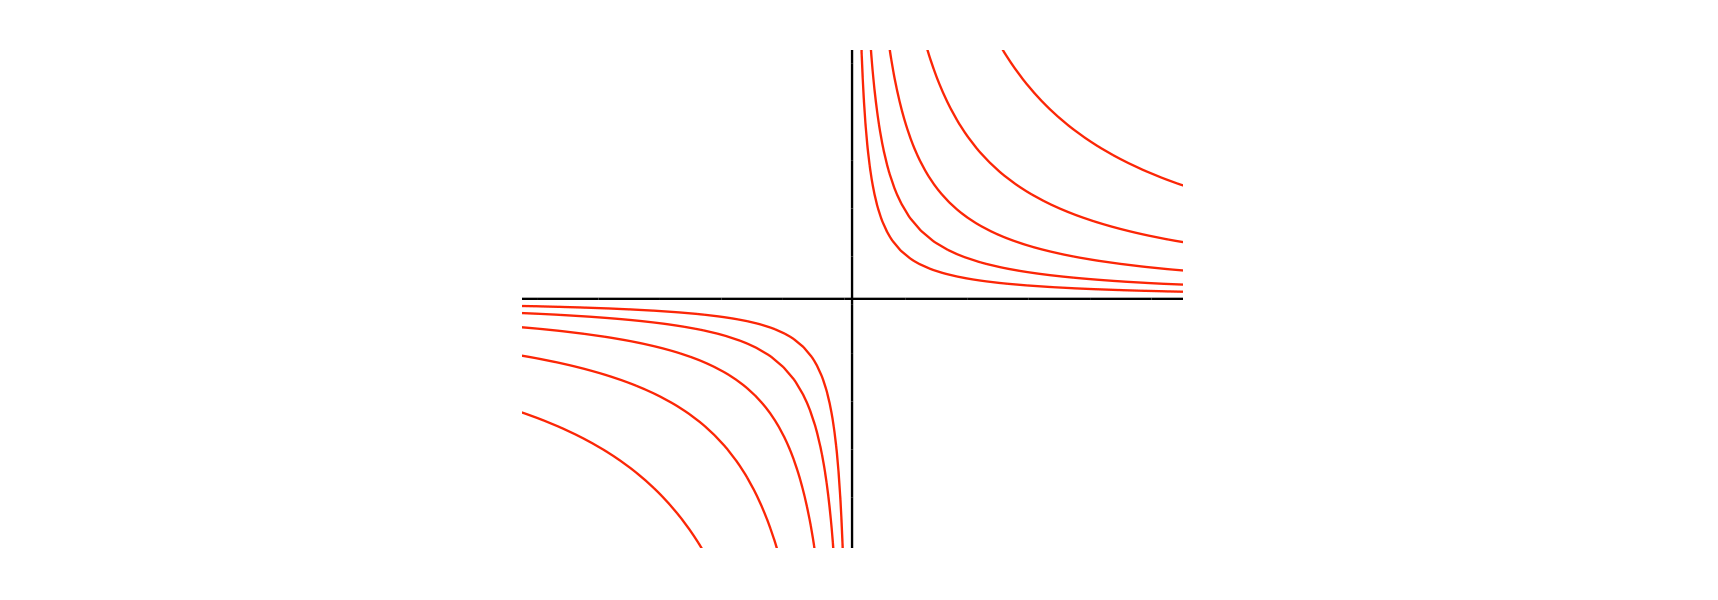
\includegraphics[width=0.62\textwidth]{figure15-1.png}
  \caption{由 $xy=t$ 切出的子空间族；$0$ 处的纤维是由 $xy=0$ 切出的 lci 空间，以黑色显示。（原文 p.~262，Figure 15.1）}
  \label{fig:15-1}
\end{figure}

一旦从光滑过渡到 lci，$T^*X[1]$ 中就出现了新的偶方向。也就是说，由于 $\mathrm{HH}^*$ 现在有对称部分，我们得到了新的非幂零方向。在这个例子中，有一个额外的 $\bA^1$ 从奇点中伸出来，如图 15.2。其想法是：若 $X$ 有奇点，则 $T^*X[1]$ 会在这些奇点上方长出新的偶方向。

\begin{figure}[htbp]
  \centering
  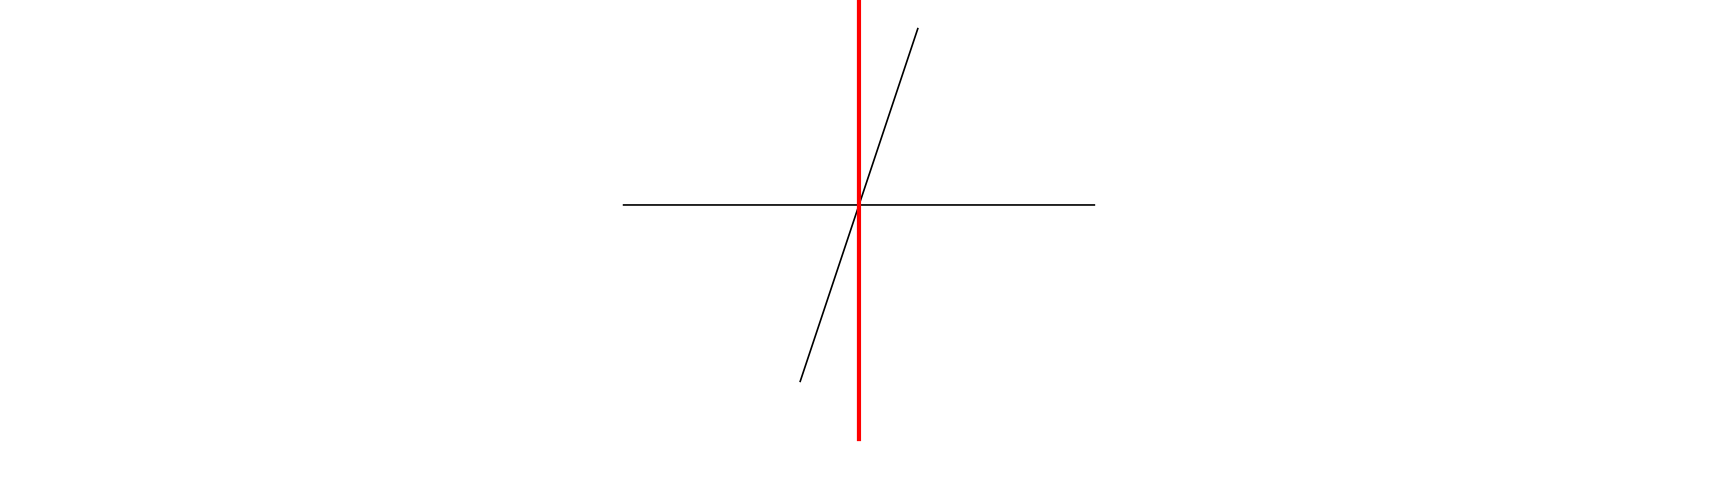
\includegraphics[width=0.42\textwidth]{figure15-2.png}
  \caption{图 15.1 所述 lci 空间的 $1$-移位余切丛的偶次数部分，在集合论意义下是奇点上方的 $\bA^1$（以红色显示）。（原文 p.~262，Figure 15.2）}
  \label{fig:15-2}
\end{figure}

这对于理解层的自同态很有帮助。但为什么理解层的自同态很重要？关于奇异簇，人们学到的一件事是：$x\in X$ 是光滑点当且仅当 $\cO_x$ 是完美复形，即它有向量丛的有限消解。而具有向量丛的有限消解等价于 $\mathrm{Ext}(\cO_x,\cO_x)$ 是有限维的。% [Tutor Note: 原文此处说 “automorphisms”，但整段讨论的是自同态（endomorphisms）$\mathrm{Ext}(\cO_x,\cO_x)$，且下文正是用 $\mathrm{Ext}$ 的无限维性刻画奇点；按上下文 “automorphisms” 应为 “endomorphisms” 的笔误。]

但若取 $\cO_0$ 的 $\mathrm{Ext}$，其中 $0$ 是 $\{xy=0\}$ 的奇点，我们得到
\begin{equation}\tag{15.60}
\mathrm{Ext}^{even}(\cO_0,\cO_0)\simeq k[t],
\end{equation}
其中变量的次数为 $|t|=2$。所以从同调代数的观点看，这个摩天楼层显得非常“无穷”，尽管它只是一个摩天楼层。关键在于：$T^*X[1]$ 中这些新的方向（如图 15.2）正是为了把这一点纳入考虑而构造的。也就是说，这个 $\mathrm{Ext}$ 恰好看起来就像 $T^*X[1]$ 中粘上的那个 $\bA^1$：
\begin{equation}\tag{15.61}
k[t]=\cO(\bA^1).
\end{equation}
用 Arinkin--Gaitsgory 的凝聚奇异支撑理论来说，$0$ 处摩天楼层的奇异支撑就是这个整个 $\bA^1$：
\begin{equation}\tag{15.62}
\mathrm{SingSupp}(\cO_0)=\bA^1.
\end{equation}
一般地，对任意凝聚层 $\cF$，可以定义（锥形）子集
\begin{equation}\tag{15.63}
\mathrm{SingSupp}(\cF)\subset T^*X[1].
\end{equation}
$\cF$ 是完美的（例如向量丛）当且仅当
\begin{equation}\tag{15.64}
\mathrm{SingSupp}(\cF)=X\hookrightarrow T^*X[1].
\end{equation}
所以奇异支撑给了我们区分有趣的凝聚层与“仅仅是向量丛”的层的方法。

\begin{srcex}{111}
设 $C$ 是亏格为 $g$ 的紧 Riemann 面，$G^\vee$ 是代数群。回想 $\Loc_{G^\vee}(C)$ 是几何 Langlands 的 $B$-侧研究的主要对象。事实证明，这个空间是 lci 的。回顾其定义为
\begin{equation}\tag{15.65}
\Loc_{G^\vee}(C):=\{\pi_1(C)\to G^\vee\}/G^\vee.
\end{equation}
映射 $\pi_1(C)\to G^\vee$ 构成的空间由纤维给出：
\begin{equation}\tag{15.66}
\begin{array}{ccc}
\{\pi_1\to G^\vee\} & \longrightarrow & (G^\vee)^{2g}\\[2pt]
\downarrow & & \downarrow{\scriptstyle \Pi_{[,]}}\\[-2pt]
1 & \longrightarrow & G^\vee
\end{array}
\end{equation}
现在我们可以处处对 $G^\vee$ 取商，得到 $\Loc_{G^\vee}$。也就是说，局部系统的空间由 $(G^\vee)^{2g}$ 经一个方程切出（模同时共轭）。这意味着 $\Loc_{G^\vee}(C)$ 上的层有很好的奇异支撑理论。
\end{srcex}
% [Tutor Note: 这里“一个方程”指 $2g$ 个元素之积的换位子等于 $1$；图中竖直箭头 $\Pi_{[,]}$ 表示把 $(g_1,\dots,g_{2g})$ 送到换位子 $\prod_i[g_i,g_{i+1}]$。$\Loc_{G^\vee}(C)$ 的 lci 性正是指它由这个截面在单位元处的纤维给出。]

于是我们发现：若考虑几何 Langlands 的 $B$-侧，则曲面 $C$ 上的四维理论 $B_{G^\vee}$（即二维理论 $B_{G^\vee}(C\times(-))$）等价于 $\Loc_{G^\vee}(C)$ 上的 $B$-模型。

回想 $B$-模型的可观测量由 $\mathrm{HH}^*$ 给出，而它产生了 $T^*X[1]$。所以 $B$-模型的状态是 $T^*X[1]$ 的某种几何量子化。换句话说，仅仅给定 $T^*X[1]$，要产生范畴 $D^b\mathrm{Coh}(X)$ 是困难的：这正是“艺术”所在。\footnote{Ludwig Faddeev 曾说：“quantization is an art, not a science.”}

\begin{srcrem}{112}
一般的拉格朗日场论必定与这幅量子化图景有关，但在 $A$-侧一切都微妙得多。这是人生经验的一个例子：$B$-侧的事情容易得多；$B$-侧为 $A$-侧的问题提供答案。在 $A$-侧我们处理局部常值映射，即拓扑；在 $B$-侧，映射不是局部常值的，而是代数或全纯映射。
\end{srcrem}

% 第 16 章 （导出）几何 Langlands 中的缺陷
% 原文：Chapter 16: (Derived) defects in Geometric Langlands
%        （pp. 265–279，印刷页码 264–278）
% 第 35 讲；2021 年 8 月 20 日
% ============================================================================
\chapter{（导出）几何 Langlands 中的缺陷}\label{ch:16}

\begin{flushright}\small 第 35 讲；2021 年 8 月 20 日\end{flushright}

\begin{keytakeaways}
本章讨论几何 Langlands 中的“导出缺陷”。先从几何 Satake 出发：线算子在 $A$-侧由 $\Shv(LG_+\backslash LG/LG_+)$ 给出，在 $B$-侧由 $\Rep(G^\vee)$ 给出；两者在导出情形下都升级为范畴。四维理论 $\cZ$ 的局部算子 $\cZ(S^3)$ 构成 $\mathbb{E}_4$-代数，线算子 $\cZ(S^2)$ 构成 $\mathbb{E}_3$-范畴，于是得到 $B$-侧的真空模空间 $\cM^1_{B_{G^\vee}}=\fg^{\vee*}[2]/G^\vee$ 及其“幂零锥”$\cM^0=\mathfrak{h}^{\vee*}[2]/W$。核心工具是 Koszul 对偶与导出自交：$\Loc_{G^\vee}(S^2)=\Omega G^\vee/G^\vee$，其上的ind-凝聚层由 $S=\mathrm{Sym}(V[-2])$ 的模刻画。由此得到 Arinkin--Gaitsgory 的奇异支撑理论以及 Beraldo 的定理：由线算子构造的可观测量正是 $T^*[1]\Loc_{G^\vee}$ 的形变量子化模。本章最后讨论余维一缺陷（畴壁与边界条件）、Langlands 函子性，以及“边界条件 $\leftrightarrow$ 移位哈密顿 $G^\vee$-空间”这一对应。
\end{keytakeaways}

\section{通过辛几何研究 TFT}
\begin{sectionkey}
本节从几何 Satake 出发：它把 $\mathcal{A}_G$ 的线算子等同于 $\mathcal{B}_{G^\vee}$ 的线算子，后者由 $\Rep(G^\vee)=\QC(\mathrm{pt}/G^\vee)$ 给出，于是（非导出）真空模空间是 $\cM^1=\mathrm{pt}/G^\vee$。由于单位线算子的自同态平凡，非导出情形下看不到局部算子；导出版本把线算子升级为 $\mathbb{E}_3$-范畴，并把真空模空间变为移位辛叠 $\fg^{\vee*}[2]/G^\vee=T^*[3](\mathrm{pt}/G^\vee)$。其来源是 $\Loc_{G^\vee}(S^2)$ 作为 $G^\vee$ 中一点的自交，即基于一点的环路空间 $\Omega G^\vee/G^\vee$，其上的层由 Koszul 对偶描述。
\end{sectionkey}

回想几何 Satake 把理论 $\mathcal{A}_G$ 中的线算子等同于理论 $\mathcal{B}_{G^\vee}$ 中的线算子。也就是说，它给出等同
\begin{equation}\tag{16.1}
\begin{array}{c}
\mathcal{A}_G(S^2)=\Shv(LG_+\backslash LG/LG_+)\\[3pt]
\big\Downarrow\\[3pt]
\mathcal{B}_{G^\vee}(S^2)=\QC(\Loc_{G^\vee}S^2).
\end{array}
\end{equation}
$B$-侧可以表达为：
\begin{equation}\tag{16.2}
\mathcal{B}_{G^\vee}(S^2)=\QC(\Loc_{G^\vee}S^2)=\QC(\mathrm{pt}/G^\vee)=\Rep(G^\vee).
\end{equation}
注意 $A$-侧 $\Shv(LG_+\backslash LG/LG_+)$ 上的乘法由卷积给出，而 $B$-侧 $\Rep(G^\vee)$ 上的乘法是张量积。

理解这个结果的一种方式是它断言：
\begin{equation}\tag{16.3}
\cM^1_B=\cM^1_A=\mathrm{pt}/G^\vee.
\end{equation}
我们还可以问这些理论中的局部算子。想法是：理论 $\cZ$ 的局部算子由 $\cZ(S^3)$ 构成；等价地，它们是单位线算子的 $\End$，即 $\cZ(S^2)=\Rep(G^\vee)$ 中平凡表示的 $\End$。其想法是，对单位取 $\End$ 是悬挂（suspension）的一种版本。但单位没有自同态：
\begin{equation}\tag{16.4}
\End_{\Rep(G^\vee)}(\mathrm{triv})=k.
\end{equation}
这是我们在几何 Langlands 中谈局部算子谈得不多的一大原因。

\begin{srcrem}{113}
今天我们不会多谈面缺陷，但它们正是分歧数据。
\end{srcrem}

\subsection{导出版本}

从物理的观点看，导出版本实际上更自然。下面是 TFT 中的一个一般法则。设 $\cZ$ 是四维 TFT。则局部算子 $\cZ(S^3)$ 构成 $\mathbb{E}_4$-代数，即某种类似奇 Poisson 代数的东西。所以它略微非交换。于是
\begin{equation}\tag{16.5}
\cM^0=\Spec\cZ(S^3)
\end{equation}
是奇 Poisson 簇。类似地，线算子构成 $\mathbb{E}_3$-代数：
\begin{equation}\tag{16.6}
\cZ(S^2),
\end{equation}
因为它附着在 $2$-球面上。不过现在它是一个范畴而非代数。所以它是一个带有并非完全交换的乘法的范畴。在阿贝尔层面，$\mathbb{E}_3$ 与对称幺半范畴相同。因此，若不进入导出情形，就“感觉不到”这种非交换性。$\mathbb{E}_2$ 无需导出就能被探测到（作为编织），但 $\mathbb{E}_3$ 不行。这个 $\mathbb{E}_4$-代数与 $\mathbb{E}_3$-范畴之间的关系是：
\begin{equation}\tag{16.7}
\cZ(S^3)=\End 1_{\cZ(S^2)}.
\end{equation}
这就是 $\mathbb{E}_n$ 与 $\mathbb{E}_m$ 之间的可加关系。% [Tutor Note: “可加关系”指把链环维数降低一维时，算子代数降一阶：$\mathbb{E}_4$-代数 $\cZ(S^3)$ 正是 $\mathbb{E}_3$-范畴 $\cZ(S^2)$ 中单位对象的自同态代数。注意 (16.6) 与 (16.7) 中 $\cZ(S^2)$ 先是范畴、后又作为对象出现，这是笔记的简写；严格写法是对范畴取单位对象 $1_{\cZ(S^2)}$。]

\begin{srcrem}{114}
我们可以照此继续，例如考虑面缺陷，它们构成 $\mathbb{E}_2$ $2$-范畴，但这里不做。
\end{srcrem}

第 $0$ 个模空间是：
\begin{equation}\tag{16.8}
\cM^0=\Spec\cZ(S^3),
\end{equation}
而由 Tannakian 重构得到的（更精细的）版本是：
\begin{equation}\tag{16.9}
\cZ^1=\text{“}\Spec\text{”}\cZ(S^2).
\end{equation}
回想 Tannakian 重构取一个张量范畴 $\cC$，构造 $\Spec\cC$，其定义为：
\begin{equation}\tag{16.10}
(\Spec\cC)(R)=\Hom_{\otimes}(\cC,R\text{-}\mathrm{mod}).
\end{equation}
现在 $R$ 是 $\mathbb{E}_4$-代数，而 $\cC$ 是 $\mathbb{E}_3$-范畴，所以谱是：
\begin{equation}\tag{16.11}
(\Spec\cC)(R)=\Hom_{\mathbb{E}_3}(\cC,R\text{-}\mathrm{mod}).
\end{equation}
也就是说，这在导出世界里说得通。$\cM^0$ 是仿射 $\mathbb{E}_4$-概形，而 $\cM^1$ 是（非仿射的）$\mathbb{E}_4$ 叠/概形。它们之间的关系是：
\begin{equation}\tag{16.12}
\cM^0=\Spec\End(1_{\cC})=\Spec\End(\cO_{\cM^1})=\Spec\Gamma(\cO_{\cM^1})=\mathrm{Aff}(\cM^1).
\end{equation}

\subsection{几何 Langlands 中的移位辛空间}

我们将聚焦 $B$-侧，因为“答案”（来自 $A$-侧）在那里。问题是：与理论 $\mathcal{B}_{G^\vee}$ 相联系的真空模空间是什么？也就是说，我们想找出：
\begin{equation}\tag{16.13}
\cM^1_{B_{G^\vee}}\to\cM^0_{B_{G^\vee}}.
\end{equation}
在非导出版本中这是：
\begin{equation}\tag{16.14}
\mathrm{pt}/G^\vee\to\mathrm{pt}.
\end{equation}
现在我们要做导出版本。

\begin{srcthm}{16}
$\cM^1_{B_{G^\vee}}=\fg^{\vee*}[2]/G^\vee$。
\end{srcthm}

也就是说，结构层是
\begin{equation}\tag{16.15}
\cO_{\cM^1_B}=\mathrm{Sym}\,\fg^\vee[-2]
\end{equation}
作为 $G^\vee$ 的表示。暂且不管移位 $2$，这在几何上是非常熟悉的东西：它是带有 $G^\vee$ 作用的余伴随表示，是表示论的基本对象之一。其推论之一是：余伴随表示带有所谓的 Kostant--Kirillov Poisson 括号，所以我们预期这里会出现某种 Poisson 几何。一种说法是：
\begin{equation}\tag{16.16}
\cM^1_B=T^*[3](\mathrm{pt}/G^\vee).
\end{equation}
这是 $3$-移位辛的，即一个 $\mathbb{P}_4/\mathbb{E}_4$ 叠。要点在于切空间是
\begin{equation}\tag{16.17}
T(\mathrm{pt}/G^\vee)=\fg^\vee[1],
\end{equation}
于是
\begin{equation}\tag{16.18}
T^*(\mathrm{pt}/G^\vee)=\fg^\vee[-1].
\end{equation}
它被 $3$-移位，所以定理中那个 $2$-移位空间实际上是按 $-1+3$ 移位的。% [Tutor Note: 这里作者把两种描述混在一起：$\cM^1_{B_{G^\vee}}=\fg^{\vee*}[2]/G^\vee$ 按定义是 $2$-移位辛的；而 $T^*[3](\mathrm{pt}/G^\vee)$ 是 $3$-移位辛的。两者的关系是 $\fg^{\vee*}[2]/G^\vee\simeq T^*[3](\mathrm{pt}/G^\vee)$：切空间 $\fg^\vee[1]$ 的余切移 $[2]$ 得 $\fg^{\vee*}[2]$，而 $\mathrm{pt}/G^\vee$ 的余切丛本身已带 $3$-移位（因为 $T(\mathrm{pt}/G^\vee)$ 在次数 $1$，余切在 $-1$，再加 $3$）。作者所说“$-1+3$”即指这个抵消。]

\subsection{它从何而来？}

考虑 $\Loc_{G^\vee}(S^2)$。我们知道 $S^2$ 可以描述为两个圆盘沿圆周粘合。由于圆盘可缩，圆盘上的局部系统实际上是平凡的：圆盘上只有一个局部系统，其自同构由 $G^\vee$ 给出。即
\begin{equation}\tag{16.19}
\Loc_{G^\vee}(D^2)=\mathrm{pt}/G^\vee.
\end{equation}
于是我们有两份 $\mathrm{pt}/G^\vee$，并想沿圆周上的局部系统粘合。但圆周上确有有意思的局部系统，因为可以有单值性（monodromy）。事实上，圆周上的局部系统由它的单值性在共轭意义下完全决定：
\begin{equation}\tag{16.20}
\Loc_{G^\vee}(S^1)=G^\vee/G^\vee.
\end{equation}
把这些放在一起得到：
\begin{equation}\tag{16.21}
\Loc_{G^\vee}(S^2)=(\mathrm{pt}/G^\vee)\times_{G^\vee/G^\vee}(\mathrm{pt}/G^\vee).
\end{equation}

\begin{srcrem}{115}
我们隐含地用了：余极限上的局部系统可以描述为各块上局部系统的极限。这是同义反复，因为可以把 $\Loc$ 看成
\begin{equation}\tag{16.22}
\Loc_{G^\vee}(-)=\Hom(-,G^\vee).
\end{equation}
\end{srcrem}

我们可以把它改写成\footnote{确实需要想一下为什么商与交可以交换。}
\begin{align}
\Loc_{G^\vee}(S^2)&=(\mathrm{pt}/G^\vee)\times_{G^\vee/G^\vee}(\mathrm{pt}/G^\vee)\tag{16.23}\\
&=(\mathrm{pt}\times_{G^\vee}\mathrm{pt})/G^\vee.\tag{16.24}
\end{align}

也就是说，$S^2$ 上的局部系统可以描述为 $G^\vee$ 中一点的自交，再模去 $G^\vee$。在阿贝尔情形，一点的自交是平凡的；但在导出情形不是。这就是所谓的\term{基于一点的环路空间}{based loop space}\footnote{要注意记号与语境：这是导出代数几何意义下的基于一点的环路，而不是同伦论中的环路空间。}，记作
\begin{equation}\tag{16.25}
\Omega G^\vee=\mathrm{pt}\times_{G^\vee}\mathrm{pt},
\end{equation}
即
\begin{equation}\tag{16.26}
\Loc_{G^\vee}(S^2)=(\mathrm{pt}\times_{G^\vee}\mathrm{pt})/G^\vee=\Omega G^\vee/G^\vee.
\end{equation}
这些环路“非常小”：它们探测不到 $G^\vee$ 的整体拓扑。事实上，它们只依赖于单位元的一个小邻域。所以若选取一些坐标，可以等同
\begin{equation}\tag{16.27}
\Loc_{G^\vee}(S^2)=(\mathrm{pt}\times_{\fg}\mathrm{pt})/G^\vee.
\end{equation}
也就是说，我们是在计算向量空间中一点的导出自交。% [Tutor Note: 这里的 $\mathrm{pt}\times_{\fg}\mathrm{pt}$ 中，$\fg$ 应理解为 $G^\vee$ 在单位元处的形式邻域（或直接取 $\fg$ 作为加群）；(16.27) 的等同只在单位元的无穷小邻域上成立，这正是“环路非常小”的含义。与 (16.25) 的差别在于把群换成了它的李代数。]

导出世界的全部要点，就是修正纤维积（特别是交）在非横截时的行为。设 $V$ 是向量空间，考虑 $0\in V$ 的导出自交：
\begin{equation}\tag{16.28}
0\cap_V0=\mathrm{pt}\times_V\mathrm{pt},
\end{equation}
即 $V$ 在 $0$ 处的基于一点的环路空间。这是导出交，但我们从记号中省略了“导出”二字。这个自交在横截性方面是“最坏的情形”：$0$ 的切空间是平凡的，所以当我们问这个交是否横截（即切空间是否张成环境空间在该点的切空间）时，会发现我们缺失了整个切空间 $T_0V\simeq V$。所以这离横截要多远有多远，但导出结构恰好会记录这一退化。

照代数几何的惯例，我们将通过其上的函数来理解这个空间。我们用到的原则是：取 $\cO$ 时，交变成张量积：
\begin{equation}\tag{16.29}
\cO(\mathrm{pt}\times_V\mathrm{pt})=k\otimes_{\cO(V)}k=k\otimes_{\mathrm{Sym}V^*}k,
\end{equation}
因为 $\cO(V)=\mathrm{Sym}V^*$。这是导出张量积，但省略记号。用 Koszul 消解可以算出这是外代数：
\begin{equation}\tag{16.30}
\cO(\mathrm{pt}\times_V\mathrm{pt})=k\otimes_{\cO(V)}k\simeq\wedge^\bullet V^*.
\end{equation}
这是一个交换（微分）分次代数（commutative (d)ga）：
\begin{equation}\tag{16.31}
\wedge^\bullet V^*=\mathrm{Sym}(V^*[1]).
\end{equation}
现在我们要计算它上的模范畴，即这个导出交 $\mathrm{pt}\times_V\mathrm{pt}$ 上的拟凝聚层。无论这个模范畴是什么，先指出它有一些结构。它会有张量积，因为它是交换环上的模；但我们对这个乘法不感兴趣。我们感兴趣的是（结合的）卷积结构。

每当我们有来自映射 $X\to Y$ 的 $X\times_YX$ 时，它就是某种以两种方式映入 $X$ 的群胚。它有卷积结构，例如当 $X$ 是有限集时，这个卷积结构就是矩阵乘法。在我们这里，$X=\mathrm{pt}$，$Y=V$。无论这个卷积结构是什么，它在 Koszul 对偶另一侧对应的运算会更明显。

为描述范畴 $\wedge^\bullet V^*\text{-}\mathrm{mod}$，我们将聚焦于我们真正理解的仅有的对象：自由模与增广模。增广模就是 $k$，其中 $\wedge^\bullet V^*\text{-}\mathrm{mod}$ 的所有外代数生成元都作用为零。它是卷积的单位。

另一种观点是：这个导出交是 $0$ 处的基于一点的环路空间：
\begin{equation}\tag{16.32}
\mathrm{pt}\times_V\mathrm{pt}=\Omega_0V.
\end{equation}
我们知道基于一点的环路空间在环路拼接下构成群（至少在某种同伦意义下）。其单位是单位元处的摩天层，即增广模。

为理解这个范畴，我们的策略如下。要研究范畴 $\cC$，可以考虑一个我们喜欢的对象 $P$，然后希望该范畴可以被描述为 $A=\Hom(P,P)$ 上的模。也就是说，有一个函子
\begin{equation}\tag{16.33}
\cC\xrightarrow{\ \Hom(P,-)\ }(\Hom(P,P))\text{-}\mathrm{mod},
\end{equation}
在好的情形下它是等价。

在我们的情形中，我们将通过计算 $\End(k)$ 来理解 $\wedge^\bullet V^*\text{-}\mathrm{mod}$。这将把我们引向 Koszul 对偶。所以需要计算：
\begin{equation}\tag{16.34}
\End_{\wedge^\bullet V^*}(k).
\end{equation}
有趣的是，$\mathrm{pt}\times_V\mathrm{pt}$ 是奇异的，即它是某种奇怪且导出的东西。如我们之前看到的，若取奇点处的摩天层，则它有无穷维自同态。也就是说，我们可以通过注意到 $k\in\wedge^\bullet V^*\text{-}\mathrm{mod}$ 不是完美的，来察觉自己在奇点处。对此的解释是：这看起来像奇异支撑上的函数，即空间在余切丛中奇点处粘上的那些额外“翅膀”上的函数。回想图 15.1 与 15.2 中的例子：节点在奇点处长出一只翅膀，用来解释摩天层的巨大自同态。这不是同一个例子，但现象相同。这就是为什么我们应当期望出现类似对称代数的东西：
\begin{equation}\tag{16.35}
\End_{\wedge^\bullet}(k)\simeq S=\mathrm{Sym}(V[-2])=\cO(V^*[2]).
\end{equation}
于是我们的空间长出了一只“翅膀”：$V^*[2]$。% [Tutor Note: 原文此处页边有手写批注“Good reference: Goresky--Kottwitz--Macpherson”。这批注指向 GKM 关于等变上同调与环面作用的经典工作；在下文的类比中，$S=\mathrm{Sym}(V[-2])$ 正是 $S^1$ 等变上同调 $H^*_{S^1}(\mathrm{pt})=k[u]$（$|u|=2$），见 (16.38)。]

这里代数内容很多。我们不会在拓扑情形下解释它。我们将把这个外代数看成：
\begin{equation}\tag{16.36}
\wedge^\bullet V^*=H_*(S^1).
\end{equation}
回想 $H_*(S^1)$ 是一个生成元上的外代数。若 $V$ 不是一维的，就把 $S^1$ 换成一个环面来想象。$(H_*(S^1),*)$ 是一个结合代数，可以称为同伦论中 $S^1$ 的群代数。对有限群，群同调字面上就是群代数。一般地，群的同调总带有结合乘法，称为 Pontrjagin 乘积。于是我们有
\begin{equation}\tag{16.37}
S=\End_{\wedge^\bullet}(k)=\End_{H_*(S^1)\text{-}\mathrm{mod}}(H^*(\mathrm{pt}))=\Hom_{S^1}(k,H^*(\mathrm{pt})).
\end{equation}
这是等变上同调的另一种说法：
\begin{equation}\tag{16.38}
S=H_{S^1}(\mathrm{pt})=H^*(BS^1\simeq\C\PP^\infty)\simeq k[u],
\end{equation}
其中 $|u|=2$。

Koszul 对偶大致是说：
\begin{equation}\tag{16.39}
\wedge^\bullet V^*\text{-}\mathrm{mod}\xrightarrow[\ \sim\ ]{\Hom_{\wedge^\bullet V^*}(k,-)}S\text{-}\mathrm{mod}.
\end{equation}
这里会遇到一些标准的技术困难。首先，必须小心我们考虑的是哪类模。例如我们可能考虑凝聚的 $\wedge^\bullet V^*$-模 $\mathrm{Coh}_\Lambda$（即有有限维上同调的有界复形），于是有范畴等价
\begin{equation}\tag{16.40}
\mathrm{Coh}_\Lambda\leftrightarrow\mathrm{Coh}_S.
\end{equation}
有趣的是，$S$ 只是对称代数，所以它看起来像向量空间上的层，而向量空间是光滑的，于是
\begin{equation}\tag{16.41}
\mathrm{Coh}_S\simeq\mathrm{Perf}_S.
\end{equation}
这非常漂亮，只不过
\begin{equation}\tag{16.42}
\mathrm{Coh}_\Lambda\neq\mathrm{Perf}_\Lambda.
\end{equation}
问题在于，增广模 $k\in\mathrm{Coh}_\Lambda$ 被送到
\begin{equation}\tag{16.43}
k\mapsto\Hom_{\wedge^\bullet V^*}(k,k)=S.
\end{equation}
但 $k$ 不是完美/紧的，而 $S\in\mathrm{Coh}_S$ 是。这一现象的另一个版本如下。我们有 $k[u,u^{-1}]\in\mathrm{Perf}_S$，它在（伴随函子下）被送到 $0\in\mathrm{Perf}_\Lambda$。所以这里有某种张力，而它由ind-凝聚层（ind-coherent sheaves）来解决。记作 $\mathrm{IndCoh}$ 或 $\QC^!$。其想法是：看奇异空间时，我们加一个叹号来提醒你得小心(!)。但要点是：
\begin{equation}\tag{16.44}
\QC^!(\mathrm{pt}\times_V\mathrm{pt})\simeq S\text{-}\mathrm{mod}.
\end{equation}
我们应把它看成对 $\Lambda\text{-}\mathrm{mod}$ 的修正/扩大：
\begin{equation}\tag{16.45}
\QC^!(\mathrm{pt}\times_V\mathrm{pt})\supset\Lambda\text{-}\mathrm{mod}=\QC(\mathrm{pt}\times_V\mathrm{pt}).
\end{equation}
其想法是：$k$ 在凝聚世界里不是紧的（行为不良），但当我们过渡到导出凝聚世界时，$k$ 变成一个紧对象（行为良好）。

无论如何，Koszul 对偶是如下形式的陈述：
\begin{equation}\tag{16.46}
(\Lambda\text{-}\mathrm{mod},*)\xrightarrow{\ \sim\ }(S\text{-}\mathrm{mod},\otimes).
\end{equation}
我们可以把它看作 Cartier/Pontrjagin 对偶的一个版本。这告诉我们：$\wedge^\bullet V^*\text{-}\mathrm{mod}$ 上的卷积结构，在通过 Koszul 对偶之后对应于一个自然出现的张量积结构。

回想在导出 Satake 的语境中，我们感兴趣的空间是
\begin{equation}\tag{16.47}
\Loc_{G^\vee}(S^2)=(\mathrm{pt}\times_{\fg^\vee}\mathrm{pt})/G^\vee.
\end{equation}

我们感兴趣的范畴是
\begin{equation}\tag{16.48}
\mathcal{B}_{G^\vee}(S^2)=\QC^!(\Loc_{G^\vee}(S^2))=\QC^!(\mathrm{pt}\times_{\fg^\vee}\mathrm{pt})^{G^\vee}.
\end{equation}
我们用 $\QC^!$ 来提醒自己正在处理奇异空间，因而把奇点处的摩天层当作“受尊重的社会成员”。回想阿贝尔版本考虑的是 $\QC(\mathrm{pt})^{G^\vee}$（或 $\QC^!$，但因为 $\mathrm{pt}$ 并不奇异，二者没有区别）；但在导出版本中我们看到，实际上应当考虑点上的导出自交上的层，而不是点本身。回到计算，我们有
\begin{equation}\tag{16.49}
\mathcal{B}_{G^\vee}(S^2)=(\mathrm{Sym}(\fg^\vee[-2]))^{G^\vee},
\end{equation}
并带张量积。对偶化后我们看到，这是（$G^\vee$-等变的）层，位于
\begin{equation}\tag{16.50}
(\fg^{\vee*}[2])/G^\vee=T^*[3](\mathrm{pt}/G^\vee).
\end{equation}

\section{局部算子}
\begin{sectionkey}
本节把“线算子的导出版本”落到局部算子上：$A$-侧局部算子为 $H^*_G(\mathrm{pt})=\mathrm{Sym}\,\mathfrak{h}^*[2]^W$，$B$-侧为 $(\mathrm{Sym}(\fg^\vee[-2]))^{G^\vee}=\mathrm{Sym}(\mathfrak{h}^\vee[-2])^W=\cO(\mathfrak{h}^\vee[2]/W)$。两者通过特征多项式映射 $\cM^1=\fg^{\vee*}[2]/G^\vee\to\cM^0=\mathfrak{h}^{\vee*}[2]/W$ 相联系，$\cM^0$ 即 Coulomb 分支。$B$-侧的关键是：这些局部算子通过“测量奇异支撑的特征多项式”作用在 $\QC^!(\Loc_{G^\vee})$ 上；限制到该映射的 $0$-纤维，就得到 Arinkin--Gaitsgory 的幂零奇异支撑范畴。
\end{sectionkey}

回想在阿贝尔故事中我们只有平凡的局部算子。让我们重新审视这一点。回想局部算子由单位线算子的自同态给出。所以这里它是 $T^*[3](\mathrm{pt}/G^\vee)$ 的仿射化。也就是说，它是
\begin{equation}\tag{16.51}
(\mathrm{Sym}(\fg^\vee[-2]))^{G^\vee}=\mathrm{Sym}(\mathfrak{h}^\vee[-2])^W=\cO(\mathfrak{h}^\vee[2]/W),
\end{equation}
其中 $\mathfrak{h}$ 是 Cartan 子代数。所以它是李代数上通常的不变量多项式空间的分次版本。换言之，我们有
\begin{equation}\tag{16.52}
\cM^1=\fg^{\vee*}[2]/G^\vee,
\end{equation}
然后还有 $\cM^0$，它通常称为（$\mathcal{N}=4$ SYM 的）\term{Coulomb 分支}{Coulomb branch}：
\begin{equation}\tag{16.53}
\cM^0=\mathfrak{h}^{\vee*}[2]/W,
\end{equation}
它们之间的映射由特征多项式映射给出：
\begin{equation}\tag{16.54}
\cM^1=\fg^{\vee*}[2]/G^\vee\to\cM^0=\mathfrak{h}^{\vee*}[2]/W.
\end{equation}
所以我们确实找到了局部算子：它们看起来正是特征多项式的系数。它们全都位于非零次数，这就是我们之前没看到它们的原因。% [Tutor Note: 这里用的是 Chevalley 限制定理：$(\mathrm{Sym}\,\fg^\vee)^{G^\vee}\cong(\mathrm{Sym}\,\mathfrak{h}^\vee)^W$，即不变多项式由其在 Cartan 上的限制决定；特征多项式映射 $\fg^{\vee*}\to\mathfrak{h}^{\vee*}/W$ 正是这一限制的几何实现。]

\subsection{$A$-侧}

既然我们有了一些非平凡的局部算子，就可以问一些问题：在实践中去哪里找它们，它们探测/做什么？这在自守侧最容易看出来。考虑 Cartan 模去 Weyl 群：
\begin{equation}\tag{16.55}
\mathfrak{h}^{\vee*}[2]/W=\mathfrak{h}[2]/W.
\end{equation}
通常方便地就把它写成 $\mathfrak{h}/W$，并只用 $\C^\times$ 作用来追踪分次。这个空间以非常自然的方式出现。回想自守 Satake 范畴是
\begin{equation}\tag{16.56}
\mathcal{A}_G(S^2)=\Shv(LG_+\backslash LG/LG_+),
\end{equation}
即仿射 Grassmann 簇上 $LG_+$-等变的层。这是某种导出怪兽，但我们只需关心卷积下的单位，即恒等陪集处的摩天层：我们有 $\mathrm{pt}\in\Gr=LG/LG_+$，并且看的是 $LG_+$-等变的层，所以单位是摩天层 $k_{\mathrm{pt}/LG_+}$。但同伦地，这个 $LG_+$ 作用与 $G$-作用相同：
\begin{equation}\tag{16.57}
k_{\mathrm{pt}/LG_+}\simeq k_{\mathrm{pt}/G}.
\end{equation}
特别地，这意味着 $A$-侧的局部算子构成
\begin{equation}\tag{16.58}
\mathcal{A}_G(S^3)=\End(1)=H^*(BG)=H^*_G(\mathrm{pt}).
\end{equation}
如同在拓扑中，
\begin{equation}\tag{16.59}
H^*_G(\mathrm{pt})=\mathrm{Sym}\,\mathfrak{h}^*[2]^W\simeq(\mathrm{Sym}\,\fg^*[2])^G.
\end{equation}
这是用冗长的方式说：$A$-侧的局部算子就是 $H^*_G(\mathrm{pt})$，即 $G$-等变上同调的系数环。这是诸如 Donaldson 理论中熟悉的东西：自然的系数环由等变上同调给出。

回想局部算子的要点是：在 $A$-侧一切都线性于它。也就是说，像 $\Shv(\Bun_G(C))$ 这样的东西可以写成对 $G$ 的商：
\begin{equation}\tag{16.60}
\Shv(\Bun_G(C))=\Shv(\Bun_G(C,x)/G),
\end{equation}
意思是它线性于 $H^*(BG)$。

\subsection{$B$-侧}

$B$-侧局部算子与线算子的导出加厚将测量奇异支撑。这正是 Arinkin--Gaitsgory 所描述的。设 $C$ 是 Riemann 面（或者干脆只是一个拓扑曲面）。$C$ 上的状态构成
\begin{equation}\tag{16.61}
\mathcal{B}_{G^\vee}(C)=\QC^!(\Loc_{G^\vee}(C)).
\end{equation}
这类层的范畴有不同模型。例如我们过去总写 $\QC$（拟凝聚层），但现在我们意识到必须更小心，要用某种ind-凝聚层，即 $\QC^!$，因为这是奇异空间。如上次所见，奇异空间上的层有奇异支撑的概念。特别地，这个空间 $\Loc_{G^\vee}(C)$ 作为纤维积出现：
\begin{equation}\tag{16.62}
\begin{array}{ccc}
\Loc_{G^\vee} & \longrightarrow & (G^\vee)^{2g}/G^\vee\\[2pt]
\downarrow & & \downarrow{\scriptstyle\Pi_{[,]}}\\[-2pt]
1/G^\vee & \longrightarrow & G^\vee/G^\vee
\end{array}
\end{equation}
它将带有来自基于一点的环路的对称性：
\begin{equation}\tag{16.63}
\Omega_1G^\vee/G^\vee\ \circlearrowleft\ \Loc_{G^\vee}.
\end{equation}
要点是：尽管 $\Loc_{G^\vee}(C)$ 不光滑，它却非常接近光滑：它是两个光滑空间之间映射的纤维。这个“翅膀”的空间，即奇异支撑所居住的地方 $T^*[1]\Loc_{G^\vee}$，看起来其实是：一个局部系统 $E$，连同 $\fg^{\vee*}[2]$ 的一个被 $E$ 扭曲的截面。无论这东西是什么，我们都可以只关心不变多项式部分：
\begin{equation}\tag{16.64}
T^*[1]\Loc_{G^\vee}\to\mathfrak{h}^{\vee*}[2]/W.
\end{equation}
这一切只是说：我们所说的局部算子 $\cO(\mathfrak{h}^{\vee*}[2])^W$ 通过测量（特征多项式意义下的）奇异支撑，作用在范畴 $\QC^!(\Loc)$ 上。

Arinkin--Gaitsgory 提出限制到这个映射的 $0$-纤维，即具有\term{幂零奇异支撑}{nilpotent singular support}的ind-凝聚层，记作
\begin{equation}\tag{16.65}
\QC^!_N(\Loc_{G^\vee}).
\end{equation}
他们这样提议，是因为它与 $A$-侧相匹配。$\Shv(\Bun_G)$ 的“显然”版本是 $H^*_G(\mathrm{pt})$-挠的。也就是说，它生活在
\begin{equation}\tag{16.66}
0\in\mathfrak{h}[2]/W=\cM^0.
\end{equation}
所以要把它与谱侧的东西匹配起来：
\begin{equation}\tag{16.67}
\Shv(\Bun_G)\stackrel{?}{\simeq}\QC^!_N(\Loc_{G^\vee}),
\end{equation}
它也应该生活在 $0$ 处。

\begin{srcthm}{17}[Beraldo]
由线算子构造的 Riemann 面 $C$ 上的可观测量构成
\[
\int_C\mathcal{B}_{G^\vee}(S^2)\simeq\mathrm{DQ}(T^*[1]\Loc_{G^\vee}),
\]
其中 $\mathrm{DQ}$ 表示“形变量子化模”，即这个空间量子化上的层。
\end{srcthm}

这是说：若用线算子作为可观测量，就能完全探测凝聚层的奇异支撑：线算子不多不少正好探测奇异支撑。可以与之前的比较：
\begin{equation}\tag{16.68}
\int_C\Rep(G^\vee)=\QC(\Loc_{G^\vee}(C)).
\end{equation}
这些是 $C$ 上“阿贝尔”线算子给出的可观测量，所以它自然地作用在下面这个范畴上：
\begin{equation}\tag{16.69}
\mathcal{A}_G(C)=\Shv(\Bun_G(C)).
\end{equation}
于是当我们从线算子过渡到导出线算子时，得到了奇异支撑。

早该说的是：导出几何 Satake 断言
\begin{equation}\tag{16.70}
\Shv(LG_+\backslash LG/LG_+)\simeq\QC^!(\Loc_{G^\vee}(S^2))=(\mathrm{Sym}(\fg^\vee[-2])\text{-}\mathrm{mod})^{G^\vee}.
\end{equation}
这是 Bezrukavnikov--Finkelberg 的定理。也就是说，导出几何 Satake 说导出线算子在 $A$-侧与 $B$-侧相同。% [Tutor Note: 原文此处有手写批注“cite”，提示补引 Bezrukavnikov--Finkelberg 关于导出几何 Satake 的工作。该定理通常表述为 $\Shv(LG_+\backslash LG/LG_+)\simeq\QC^!(\Loc_{G^\vee}(S^2))$，等价于 $\fg^{\vee*}[2]/G^\vee$ 上的ind-凝聚层；右端的 $(\mathrm{Sym}(\fg^\vee[-2])\text{-}\mathrm{mod})^{G^\vee}$ 是对偶描述。]

所以要点是：由于 $\Loc_{G^\vee}C$ 奇异，线算子的导出版本在谱意义上分解于 $T^*[1]\Loc_{G^\vee}$ 之上。
% [Tutor Note: 原文 "the derived version of line operators spectrally composes over $T^*[1]\Loc_{G^\vee}$
%  里的 composes 不好直译。作者在全书表述这类谱分解时一律用 spectrally decomposes
%  （第 1、3、10、11、13、14、15 章共 14 处），此处 composes 应是 decompose 的笔误或口语变体。
%  译文按 "分解于 $T^*[1]\Loc_{G^\vee}$ 之上" 处理，即导出线算子按该处的奇异支撑来组织。
%  [译者按（无外部依据）：依据是作者他处的一致用法与本章语境，未找到外部文献佐证。]]

\begin{srcrem}{116}
光滑点就是所谓的\term{尖点 Langlands 参数}{cuspidal Langlands parameters}。所以整套奇异支撑理论告诉你如何理解非尖点的 Langlands 参数。
\end{srcrem}

\section{边界条件（余维一缺陷）}
\begin{sectionkey}
本节讨论余维一缺陷：它们把流形分成两部分，因而自然地充当两个场论之间的“映射”。把两张理论拼起来的畴壁，可以通过沿畴壁“折叠”而看成单一理论 $Z\otimes Z'$ 的边界条件。由此，Langlands 函子性（群同态 $H^\vee\to G^\vee$ 诱导 $B_{H^\vee}\to B_{G^\vee}$ 的畴壁）成为边界条件的一个特例。最后的结论是：$B_{G^\vee}$ 的边界条件大致对应于（移位的）哈密顿 $G^\vee$-空间。
\end{sectionkey}

到目前为止我们谈了点（局部）算子、线算子和面算子。现在来谈余维一算子/缺陷。我们可以考虑两类不同的余维一缺陷。与早先的缺陷概念不同，余维一缺陷自然把流形分成两部分。你可以谈边界，或嵌入的余维一子流形。在物理中它们被称为\term{畴壁}{domain walls}。因为空间被分成两部分，畴壁一般就是把两个不同的场论 $\cZ$ 与 $\cZ'$ 分隔开的东西。场论之间最自然的映射概念之一就是畴壁，即应把分隔两个理论的畴壁看成从一个理论到另一个理论的映射。形式地说，我们把定义在通常配边上的理论推广到定义在二分（bipartite）流形上。也就是说，从 $\cZ$ 到 $\cZ'$ 的映射，是把两者都延拓到二分流形上定义的，其中一侧是 $\cZ$，另一侧是 $\cZ'$。

\subsection{Langlands 函子性}

我们不打算把 $A$-侧与 $B$-侧的理论联系起来，尽管可以这样想：Langlands 对应本身就由某个神奇的畴壁给出。相反，我们将做下面这件事。谈 Langlands 函子性时，人们说的是：对两个不同的群 $G^\vee$ 与 $H^\vee$，我们可能试图把 $\mathcal{B}_{G^\vee}$ 与 $\mathcal{B}_{H^\vee}$ 联系起来。最显然的做法（这也正是人们通常所说的 Langlands 函子性）是取一个子群 $H^\vee\subset G^\vee$，然后构造映射
\begin{equation}\tag{16.71}
\mathcal{B}_{H^\vee}\to\mathcal{B}_{G^\vee}.
\end{equation}
特别地，若看 Riemann 面 $C$ 上的局部系统，就得到一个真正的映射
\begin{equation}\tag{16.72}
\Loc_{H^\vee}(C)\to\Loc_{G^\vee}(C),
\end{equation}
它诱导出前推函子
\begin{equation}\tag{16.73}
\QC^!(\Loc_{H^\vee}(C))\to\QC^!(\Loc_{G^\vee}(C)).
\end{equation}
我们没有用到 $C$ 是 Riemann 面。事实上这可以延拓到整个场论。我们甚至没有用到它是个子群，所以完全可以从群同态 $H^\vee\to G^\vee$ 出发。于是 Langlands 函子性问的是：这在 $A$-侧对应什么：
\begin{equation}\tag{16.74}
\begin{array}{ccc}
\mathcal{B}_{H^\vee} & \longrightarrow & \mathcal{B}_{G^\vee}\\[2pt]
\wr & & \wr\\[2pt]
\mathcal{A}_H & \stackrel{?}{\dashrightarrow} & \mathcal{A}_G
\end{array}
\end{equation}
% [Tutor Note: (16.74) 是 Langlands 函子性的图示：中间一行的两个 $\wr$ 表示上下两行对象在几何 Langlands 对偶下相互对应（左侧 $H$-那一对、右侧 $G$-那一对），底行 $\mathcal{A}_H$ 到 $\mathcal{A}_G$ 的虚线加“?”表示这个函子既未构造、也未必存在——正如紧接的正文所说，$H^\vee\to G^\vee$ 并不给出任何形式的映射 $H\to G$。[译者按（无外部依据）：依 (16.71)–(16.73) 与下一句推得。]]
问题在于，$H^\vee\to G^\vee$ 并不给出任何形式的映射 $H\to G$。

这实际上更接近 Langlands 最初表述纲领的方式。也就是说，存在某个 Langlands 函子性原则，它不精确地说：对任何映射 $H^\vee\to G^\vee$，都应存在一个从 $H$ 的自守形式到 $G$ 的自守形式的操作。% [Tutor Note: 原文明明讨论的是 automorphic forms（自守形式），但抽取文本两处都写作 “automorphism forms”（自同构形式），这是笔误；译文按“自守形式”处理。]

这类函子性的另一个关键例子是抛物诱导/Eisenstein 级数理论。在这个语境中，给定群 $G^\vee$，然后取极大环面 $T^\vee$。

\begin{figure}[htbp]
  \centering
  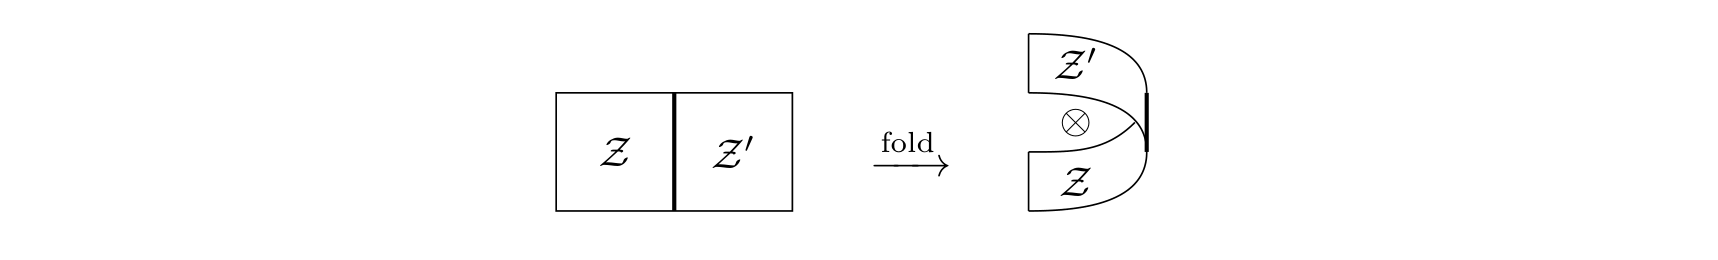
\includegraphics[width=0.72\textwidth]{figure16-1.png}
  \caption{沿畴壁“折叠”后，我们可以把 $\cZ$ 与 $\cZ'$ 之间的畴壁看作张量积 $\cZ\otimes\cZ'$。（原文 p.~275，Figure 16.1）}
  \label{fig:16-1}
\end{figure}

我们可以把它看成一个子群，但这里我们改为把 Borel 子群看成在这两者之间进行插值：
\begin{equation}\tag{16.75}
\begin{array}{ccc}
& B^\vee &\\
\swarrow & & \searrow\\
G^\vee & & T^\vee
\end{array}
\end{equation}
这给出 $\mathcal{B}_{G^\vee}$ 与 $\mathcal{B}_{T^\vee}$ 之间的畴壁。例如在 Riemann 面 $C$ 上，我们得到一个对应：
\begin{equation}\tag{16.76}
\begin{array}{ccc}
& \Loc_{B^\vee}(C) &\\
\swarrow & & \searrow\\
\Loc_{G^\vee}(C) & & \Loc_{T^\vee}(C)
\end{array}
\end{equation}
$\Loc_{B^\vee}(C)$ 由带旗的 $G^\vee$-局部系统构成。于是有一个自然的操作，从 $\Loc_{G^\vee}$ 得到 $\Loc_{T^\vee}$：拉回与前推。在这种情形下，我们其实知道另一侧该怎么做：我们同样想
\begin{equation}\tag{16.77}
G\supset B\twoheadrightarrow T,
\end{equation}
于是得到对应
\begin{equation}\tag{16.78}
\begin{array}{ccc}
& \Bun_B &\\
\swarrow & & \searrow\\
\Bun_G & & \Bun_T
\end{array}
\end{equation}
所以我们又可以拉回与前推。

\subsection{畴壁与边界条件}

现在稍微换一个视角。双模 ${}_AM_B$ 等同于 $A\otimes B^{\mathrm{op}}$ 上的模。在线性代数中，这只是说映射 $f:V\to W$ 等同于元素 $f\in V^*\otimes W$。所以我们取双模 ${}_AM_B$，可以把它看成一个函子
\begin{equation}\tag{16.79}
{}_AM_B:A\text{-}\mathrm{mod}\to B\text{-}\mathrm{mod},
\end{equation}
并等价地把它看成 $A\otimes B^{\mathrm{op}}\text{-}\mathrm{mod}$ 的元素。

直观地说，与其考虑双模/畴壁，我们将像图 16.1 那样把纸张折叠起来。边界条件就是到平凡理论的畴壁。所以，与其把余维一缺陷看成从 $\cZ$ 到 $\cZ'$ 的畴壁/映射，我们把它看成单一理论 $\cZ\otimes\cZ'$ 的边界条件。要点是：畴壁（或函子性）是边界条件的特例。

例如，在这个 Eisenstein 级数的例子里，与其把畴壁看成由 $B$ 给出：
\begin{equation}\tag{16.80}
G\supset B\twoheadrightarrow T,
\end{equation}
我们可以把它折过来，把 $B$ 看成 $G\times T$ 理论的边界条件。或者可以几何地看。若有
\begin{equation}\tag{16.81}
U\hookrightarrow B\twoheadrightarrow T,
\end{equation}
则 $G/U$ 是一个带有两个作用的空间：
\begin{equation}\tag{16.82}
G\ \circlearrowleft\ G/U\ \circlearrowright\ T.
\end{equation}
然后对群取商，就得到
\begin{equation}\tag{16.83}
\begin{array}{ccc}
& \mathrm{pt}/B &\\
\swarrow & & \searrow\\
\mathrm{pt}/G & & \mathrm{pt}/T
\end{array}
\end{equation}
要点是：我们可以只关注边界条件，而不必操心畴壁。

\subsection{哈密顿作用}

要点将是下面这个。

\begin{srcclaim}{3}
$\mathcal{B}_{G^\vee}$ 的边界条件大致等同于/给出一个（移位的）哈密顿 $G^\vee$-空间。
\end{srcclaim}

这是 Coulomb 分支理论（Braverman--Finkelberg--Nakajima）的一个版本，它早先已在物理语境中出现，例如 Gaiotto--Witten。% [Tutor Note: 原文此处页边有手写批注“cite BFN and GW”，提示补引 Braverman--Finkelberg--Nakajima（Coulomb 分支）与 Gaiotto--Witten（边界条件与规范理论）的文献。译文正文保留了对这两项工作的提及。]

\begin{srcex}{112}
设 $G$ 是群，$X$ 是 $G$-空间。现在考虑 $T^*X$。它是辛的，并从 $X$ 得到 $G$ 的作用，但它还有一个矩映射
\begin{equation}\tag{16.84}
T^*X\to\fg^*,
\end{equation}
它是 $G$-等变的。这个矩映射给出 $\mathrm{Lie}(G)=\fg$-作用的哈密顿量。其想法是，映射 $T^*X\to\fg^*$ 给出函数上的映射
\begin{equation}\tag{16.85}
H:\cO(\fg^*)=\mathrm{Sym}\,\fg\to\cO(T^*X),
\end{equation}
即哈密顿算子。于是对 $x\in\fg$，可以看对应的哈密顿函数 $H_x\in\cO(T^*X)$；说它对作用而言是哈密顿的，就是说与 $H_x$ 的 Poisson 括号等同于 $x$ 的作用：
\begin{equation}\tag{16.86}
\{H_x,-\}=\text{action of }x\text{ on }T^*X.
\end{equation}
\end{srcex}

于是我们有一个映射 $\fg\to\cO(T^*M)$，它提升 $\fg$ 到向量场的映射：
\begin{equation}\tag{16.87}
\begin{array}{ccc}
\mathrm{Sym}\,\fg & \xrightarrow{\ H\ } & \cO(T^*M)\\[2pt]
\uparrow{\scriptstyle\iota} & & \downarrow{\scriptstyle\{,-\}}\\[2pt]
\fg & \xrightarrow{\ \text{action}\ } & \mathrm{Vect}(T^*M)
\end{array}
\end{equation}
% [Tutor Note: 原图是一幅不太规整的草图：$\mathrm{Sym}\,\fg$ 有斜箭头分别指向 $\cO(T^*M)$ 与 $\mathrm{Vect}(T^*M)$，$\fg$ 有箭头指向 $\mathrm{Vect}(T^*M)$。这里按数学含义重排为交换方块：上横为 (16.85) 的 $H$，右竖为“取哈密顿向量场”（Poisson 括号），下横为 $G$-作用，左竖为 $\fg\hookrightarrow\mathrm{Sym}\,\fg$。]

现在若给定任意带 $G$-作用的辛空间 $M$（即不一定形如 $T^*X$），我们可以要求同样的数据：
\begin{equation}\tag{16.88}
\begin{array}{ccc}
M & \longrightarrow & \fg^*\\[2pt]
\circlearrowleft & {\scriptstyle G} & \circlearrowright
\end{array}
\end{equation}
即一个到 $\fg^*$ 的映射，对群等变，生成 $G$ 的李代数作用，且与辛结构相容。

我们已经看到某种应当让我们想起几何 Satake 的东西。我们可以把这组数据重新表述为叠的映射：
\begin{equation}\tag{16.89}
M/G\xrightarrow{\ \mu\ }\fg^*/G.
\end{equation}
除去分次问题（例如我们或许会期望 $\fg^*[2]/G$），矩映射的目标看起来像 $B$-理论的真空模空间：
\begin{equation}\tag{16.90}
M/G\xrightarrow{\ \mu\ }\fg^*[2]/G=\cM^1_B.
\end{equation}
所以哈密顿几何切入的地方在于：到 $\cM^1_B$ 的映射会非常接近哈密顿 $G$-作用。因此我们希望从边界条件中提取出看起来像哈密顿作用的数据。

让我们再做些场论缺陷学。想法是做同样的谱废话。我们这样总结：给定 TFT $\cZ$ 的一个边界条件 $T$，我们想提取算子代数并取 $\Spec$。这将得到空间 $M$，而在我们的情形中它将是哈密顿空间。所以断言是：这个空间生活在理论 $\cZ$ 的真空模空间之上。也就是说，我们已经取了一个理论 $\cZ$ 并从中造出代数几何；现在我们要为一个理论 $\cZ$ 连同边界条件 $T$ 一并造代数几何。

回想我们对二维理论做过类似的事。若有一个范畴 $\cC$（我们把它看成对应二维 TFT），可以考虑一个对象 $\cF\in\cC$。然后看 $\cF$ 的自同态代数，它接收来自二维理论 $\cZ$ 的局部算子的映射：
\begin{equation}\tag{16.91}
\mathrm{HH}(\cC)=\cZ(S^1)\to\End(\cF).
\end{equation}
于是我们有一个局部算子上的代数，即它层化在局部算子的 $\Spec$ 上，奇异支撑正是由此而来。

用代数的语言重复这一点：有一个代数 $A$ 作用在模 $M$ 上，由此得到映射
\begin{equation}\tag{16.92}
\mathrm{center}(A)\to\End(M),
\end{equation}
这就是我们将要得到的那类东西。在此情形中 $\End(M)$ 只是结合（$\mathbb{E}_1$）代数，所以其实不太想对它取 $\Spec$，因为它不够交换。但在四维中一切都更交换。于是我们可以取 $\Spec$ 并看到几何。

设 $\cZ$ 是四维 TFT，$T$ 是边界条件。为热身，先假设 $\cZ$ 平凡。这种情形下 $T$ 等同于一个通常的三维 TFT。那么 $T$ 的局部算子 $\mathcal{T}(S^2)$ 构成 $\mathbb{E}_3$-代数。在上同调层面它看起来只是一个（分次的、偶的）Poisson 代数。于是可以定义这个理论 $T$ 的真空模空间为
\begin{equation}\tag{16.93}
\cM^0_T=\Spec\bigl(\mathcal{T}(S^2)\bigr),
\end{equation}
我们可以把它看成（仿射的）Poisson 簇。若取一个带 $\C^\times$ 作用的普通 Poisson 簇，则其函数环是分次的，我们可以把该分次宣布为上同调分次。也就是说，取使 $\{,\}$ 的次数为 $-2$ 的 $\C^\times$-作用。所以这是一个 $\mathbb{P}_3$-簇。

\begin{srcex}{113}
$T^*X$ 总有 $\C^\times$ 的伸缩作用。它的次数为 $2$，所以其逆——Poisson 括号——的次数为 $-2$。也就是说，我们可以把它做成 $\mathbb{P}_3$-簇。
\end{srcex}

模空间 $\cM^0_T$ 总是仿射的，因为我们只看了局部算子。改而看线算子 $\mathcal{T}(S^1)$，它是 $\mathbb{E}_2$-范畴（编织的）。所得的模空间将是一个不一定仿射的 $\mathbb{E}_3$-叠。我们正在做某种（从理论 $T$ 重构 $M$ 的）重构，但也许反过来想更容易。若从分次辛的 $M$ 出发（即带有 $\C^\times$-作用，使辛形式的权为 $2$），则可以构造一个三维 TFT，称为 \term{Rozansky--Witten 理论}{Rozansky--Witten theory}。该理论的局部算子构成
\begin{equation}\tag{16.94}
\mathcal{T}_M(S^2)=(\cO(M),\{,\}),
\end{equation}
把它看成 $\mathbb{P}_3$-代数；而线算子是
\begin{equation}\tag{16.95}
\mathcal{T}_M(S^1)=\QC(M).
\end{equation}
但线算子上的张量积其实带有编织形变，所以它实际上是 $\mathbb{E}_2$ 的。这一点真正被理解的只有 $M=T^*X$ 的情形，此时我们其实用的是 Koszul 对偶：
\begin{equation}\tag{16.96}
\QC(T^*X)\leftrightarrow\QC^!(LX),
\end{equation}
而 $\QC^!(LX)$ 带有自然的 $\mathbb{E}_2$-结构。

于是我们从 $T$ 出发，得到
\begin{equation}\tag{16.97}
\cM^1\to\cM^0,
\end{equation}
然后希望 $T$ 是 $\cM^0$ 上的 RW，更可能是 $\cM^1$ 上的 RW。

\begin{srcrem}{117}
物理学家可能把这些模空间之一的 RW 称为 $T$ 的低能有效场论。
\end{srcrem}

\par\medskip\noindent\textbf{警告 3.}\ 这种重构有时会惨败。例如考虑 Chern--Simons。它没有局部算子，所以仿射版本会是一个点。它有有意思的线算子，由这个模张量范畴给出，但若试图取它的谱，也只是一个点。这个模张量范畴没有任何导出的东西，所以它无法与 $\mathbb{E}_3$-代数对话。然而 $BG$ 由 Killing 型给出 $2$-移位辛结构，而 Chern--Simons 在道德上就是 $BG$ 的 RW，但我们从 $\cM^0$ 和 $\cM^1$ 都看不到这一点。% [Tutor Note: 原文 “the BG” 指分类叠 $BG$；“killing form” 应为首字母大写的 Killing 型。此处作者强调：Chern--Simons 的线算子范畴（模张量范畴）是半单的、没有导出结构，因此不能用局部算子/线算子的谱重构出 $BG$ 的 $2$-移位辛几何；这说明本节的重构程序并非普遍适用。]

现在设我们的体理论 $\cZ$ 非平凡，仍带边界条件 $T$。要点是：我们刚才所说的一切都有相对版本。也就是说，$T$ 的局部算子 $\mathcal{T}(S^2)$ 不再是像之前那样的裸 $\mathbb{E}_3$-代数，而是范畴 $\cZ(S^2)$ 中的 $\mathbb{E}_3$-代数。一种说法是：我们可以取体中的局部算子并把它们与边界碰撞，使 $\mathcal{T}(S^2)$ 成为 $\cZ(S^3)$ 上的代数。这类似于早先的情形：若有一个模 $A\ \circlearrowleft\ M$，则 $\End(M)$ 是 $A$ 的中心上的代数。也就是说，它是范畴 $\mathrm{center}(A)\text{-}\mathrm{mod}$ 中的（$\mathbb{E}_1$）代数对象。谈论这个范畴的代数对象是合理的，因为 $A$ 的中心是 $\mathbb{E}_2$，所以它上的模范畴本身就是 $\mathbb{E}_1$ 的。

同样的图景在三维理论中也成立：边界上的局部算子 $\mathcal{T}(S^2)$ 是 $\mathbb{E}_4$-代数 $\cZ(S^3)$ 上的 $\mathbb{E}_3$-代数，即 $\mathbb{E}_3$-范畴 $\cZ(S^3)\text{-}\mathrm{mod}$ 中的 $\mathbb{E}_3$-代数对象。现在我们处于更交换的环境，可以取 $\Spec$。这意味着我们有一个映射
\begin{equation}\tag{16.98}
\begin{array}{c}
\Spec\mathcal{T}(S^2)\\[2pt]
\downarrow\\[2pt]
\cM^0=\Spec\cZ(S^3)
\end{array}
\end{equation}
这个映射是所谓拉格朗日映射的一个例子（它与 Poisson 结构有某种相容性）。范畴 $\cZ(S^3)\text{-}\mathrm{mod}$ 其实是对 $\cZ(S^2)$ 的近似。更好的想法是：$\mathcal{T}(S^2)$ 是 $\mathbb{E}_3$-范畴 $\cZ(S^2)$ 中的 $\mathbb{E}_3$-代数对象。

若身处 Langlands 语境，即体理论 $\cZ$ 实际上是 $\mathcal{B}_{G^\vee}$，我们看到：对 $\mathcal{B}_{G^\vee}$ 的边界理论 $T$，我们得到 $\fg^{\vee*}[2]/G^\vee$ 上的代数，因为这个范畴 $\cZ(S^2)$ 是余伴随表示 $\fg^{\vee*}[2]/G^\vee$ 上的层。于是取 $\Spec$ 时，得到一个仿射态射
\begin{equation}\tag{16.99}
M/G^\vee\to\fg^{\vee*}[2]/G^\vee,
\end{equation}
它与 Poisson 结构相容。这等同于给出一个仿射哈密顿 $G^\vee$-簇（在分次剪切意义下）$G^\vee\ \circlearrowleft\ M$。然后若想看到非仿射的东西，可以看 $\mathcal{T}(S^1)$，它是 $\cZ(S^2)$ 上的 $\mathbb{E}_2$-代数。于是我们得到类似
\begin{equation}\tag{16.100}
\QC(M/G^\vee)
\end{equation}
的东西，它被
\begin{equation}\tag{16.101}
\QC(\fg^{\vee*}[2]/G^\vee)
\end{equation}
通过矩映射作用。所以 $\mathcal{B}_{G^\vee}$ 的边界条件以哈密顿 $G^\vee$-空间作为其“影子”。反过来，若 $G^\vee\ \circlearrowleft\ M$ 是全纯辛簇上的哈密顿作用，则 $\mathrm{RW}_M$ 定义了 $\mathcal{B}_{G^\vee}$ 的一个边界条件。

% ============================================================================
%  第 17 章  几何 Langlands 中的边界条件
% ============================================================================
\chapter{几何 Langlands 中的边界条件}\label{ch:17}

\begin{flushright}
\small 第 36 讲；2021 年 8 月 24 日
\end{flushright}

具体地，我们将讨论几何 Langlands 中的边界条件在数论中的应用。

\begin{keytakeaways}
本章说明如何用几何 Langlands 中的边界条件统一处理 $L$-函数与周期。基本想法是：
$n$ 维规范场论的边界条件大致等同于带 $G$-对称的 $(n-1)$ 维理论；对四维 $\mathcal N=4$
超杨--Mills 理论，边界条件给出三维理论，其局部算子构成 $E_3$-代数，取相对谱便得到对偶群的
哈密顿空间。B-侧的边界条件（以哈密顿 $G^{\vee}$-空间 $M^{\vee}$ 为靶的 Rozansky--Witten 理论）
组织 Galois 表示的 $L$-函数：局部 $L$-因子是 Frobenius 在 $\operatorname{Sym}^{\bullet}V=\cO(M^{\vee})$
上的迹，整体 $L$-函数则是 $L$-可观测层的因子化同调（沿曲线取迹）。A-侧的边界条件
（球簇 $X$ 的余切丛 $T^*X$ 等哈密顿 $G$-空间）组织自守形式的周期，Plancherel 测度在几何上范畴化为
$M^{\vee}$。两者通过猜想 $|\mathcal{P}_X(\varphi)|^2=L(\rho,M^{\vee})$ 相联系。核心工具包括：相对谱、
因子化同调、几何 Satake、球簇、Iwasawa--Tate 理论以及 Hecke 代数与 $\Rep(G^{\vee})$ 的等价。
\end{keytakeaways}

\section{边界条件概述}

\begin{sectionkey}
本节给出全章的总图景：$n$ 维规范场论的边界条件是带 $G$-对称的 $(n-1)$ 维理论；对四维
$\mathcal N=4$ 超杨--Mills，A/B 扭转给出两类边界条件，而电磁对偶把 $G$ 的边界条件与
$G^{\vee}$ 的边界条件对应起来。由此，A-侧的哈密顿 $G$-空间与 B-侧的哈密顿 $G^{\vee}$-空间应当互相匹配。
\end{sectionkey}

粗略的想法是：$n$ 维规范场论（规范群为 $G$）的边界条件，大致应该是带 $G$-对称的
$(n-1)$ 维理论。首先我们举一些例子，作为真正关心的问题的热身。

\begin{srcex}{114}
若 $G$ 是紧 Lie 群，则存在一个二维 QFT，即拓扑杨--Mills 理论 $\mathrm{YM}^{top}_G$。
其边界条件是一维理论，现在带 $G$-对称，故边界条件的范畴是 $\Rep(G)$。
\end{srcex}

\begin{srcex}{115}
二维 A-型规范场论也被物理学家称为群 $G$ 在 A-扭转下的 $\mathcal N=(2,2)$ 超杨--Mills 理论。
我们如下给出该理论的边界条件。设 $G\curvearrowright X$。边界理论将是某种量子力学；
但代替 $X$ 上的普通量子力学，我们可以通过把 de Rham 复形 $H^{\bullet}_{dR}(X)$ 作为态空间，
在 $X$ 上做超对称量子力学。由于 $G\curvearrowright X$，我们可以问 de Rham 复形获得何种对称性。
它确实有作用，但方式使得 $\mathfrak g=\mathrm{Lie}(G)$ 的作用被平凡化。这正是著名的
Cartan 同伦恒等式的内容。故经典地，你只看到连通分量群在作用；但更丰富的说法是，事实上得到作用
\begin{equation}\tag{17.1}\label{eq:17.1}
H_*(G)\curvearrowright H^*(X).
\end{equation}
这些可以称为 $G$ 的\term{局部常值表示}{locally constant representation}，
而不是上一个例子中那样的普通表示。
\end{srcex}

这与我们将在四维 A-模型中看到的情形非常相似。特别地，这个理论中的局部算子看起来像
\begin{equation}\tag{17.2}\label{eq:17.2}
H_*(G)\otimes H^*(BG).
\end{equation}

% [Tutor Note: 式 (17.1) 中的 $H_*(G)$ 作用是 Cartan 模型给出的：$G$ 在 de Rham 复形上的
%  作用可同伦平凡化，从而在 $H^*(X)$ 上只剩 $H_*(G)$（即 $G$ 的链复形/群同调）的作用；
%  这就是为什么作者称其为“局部常值表示”而不是普通表示。对连通紧群，$H_*(G)\cong H^*(\Omega G)$，
%  它与 $H^*(BG)$ 通过 Koszul 对偶相关联，于是 (17.2) 中 $H_*(G)\otimes H^*(BG)$ 正是
%  $G$-等变上同调在自由作用情形下的局部模型。注意不要把 $H_*(G)$ 与群环 $\C[G]$ 混淆。]

在几何 Langlands 中，我们研究这个物理规范场论的边界条件，它称为四维
$\mathcal N=4$ 超杨--Mills 理论（Gaiotto--Witten），是一个 $G$-规范理论。
一个边界条件（原文此处标注 cite）是某种带 $G$-对称的三维理论。因为我们讨论的是超对称的
体理论，所以也需要适当超对称的边界理论。在物理中，若取一个流形 $M$，它不仅具有 Riemann 度量
（如 SUSY QM 所需），也不仅具有 Kähler 结构，而具有\term{超 Kähler}{hyperkähler}结构，
那么这恰好就是构造到 $M$ 的三维 $\sigma$-模型所需的条件。这最终是一个 $\mathcal N=4$
超对称理论（即有 8 个超荷）。我们应把它看作\term{2-移位量子化}{2-shifted quantization}的版本：
我们构造的不再是向量空间（即一维场论），而是三维 QFT。由于有足够的超对称，我们可以用几种方式
使它拓扑化。一种是“Coulomb”/B-扭转，给出以 $M$ 为靶的 Rozansky--Witten TFT。
还有“Higgs”/A-扭转，即鲜为人知的三维 A-模型。我们不打算真正讨论 A-模型。
超 Kähler 流形有很多结构，但特别地它是全纯辛的。对 Rozansky--Witten 理论，我们只需要 $M$
是全纯辛的，即实际上不需要 Riemann 度量。

设有一个紧群 $G_c$ 通过超 Kähler 等距作用 $G_c\curvearrowright M$。（或者我们可以考虑复群
$G_{\C}$ 通过全纯辛对称性作用 $G_{\C}\curvearrowright M$。）由这些数据，我们得到这个四维
$\mathcal N=4$ 杨--Mills 理论的一个边界条件。确实，类型是匹配的：A-型版本给出四维 A-理论
$\mathcal A_G$ 的边界条件，B-型版本给出四维 B-理论 $\mathcal B_G$ 的边界条件。
这将是我们边界理论的来源。

Gaiotto 与 Witten 告诉我们：若你有电磁/S-对偶，那么它是把 $G$ 的 $\mathcal N=4$ SYM 与
$G^{\vee}$ 的 $\mathcal N=4$ SYM 等同起来的对称性。既然理论本身被等同，边界条件也被等同。
于是我们得到 $\mathcal A_G$ 的边界条件与 $\mathcal B_{G^{\vee}}$ 的边界条件之间的对应。
在 $\mathcal A_G$ 的边界条件中，可以考虑“几何的”那些，它们来自哈密顿 $G$-空间
$G\curvearrowright M$。于是我们可能希望它们与来自哈密顿 $G^{\vee}$-空间
$G^{\vee}\curvearrowright M^{\vee}$ 的 Rozansky--Witten 理论相匹配。我们甚至可以更贪心一些，
希望真正匹配 A-侧上为余切丛的那些：
\begin{equation}\tag{17.3}\label{eq:17.3}
G\curvearrowright X;\quad M=T^*X
\qquad\overset{?}{\longleftrightarrow}\qquad
G^{\vee}\curvearrowright X^{\vee};\quad M^{\vee}=T^*X^{\vee}.
\end{equation}

\section{相对谱}

\begin{sectionkey}
本节说明：给定四维 TFT 的边界理论 $\mathcal T$，它在每个配边上给出一个元素
$\mathcal T(N)\in\cZ(N)$；对 $S^2$ 取这个元素，得到线算子范畴中的 $E_3$-代数，
其谱给出对偶群上的哈密顿空间 $M^{\vee}\to\mathfrak g^{\vee*}/G^{\vee}$，即“相对谱”。
\end{sectionkey}

回忆上次的内容：我们可以做得更好一些——给定一个边界条件，实际上可以构造一个哈密顿
$G$-空间或 $G^{\vee}$-空间。这就是“相对谱”构造。

设 $\cZ$ 是四维 TFT，边界理论/条件为 $\mathcal T$。这给出什么样的代数结构？
我们可以把 $\mathcal T$ 想成从平凡理论到 $\cZ$ 的映射：
\begin{equation}\tag{17.4}\label{eq:17.4}
\mathcal T\in\Hom(1,\cZ).
\end{equation}
这意味着，对维数 $\le 3$ 的 $N$，可以看 $\cZ(N)$，并得到
\begin{equation}\tag{17.5}\label{eq:17.5}
\mathcal T(N)\in\Hom\bigl(1,\cZ(N)\bigr).
\end{equation}
我们确实可以把它理解为定义了一个元素
\begin{equation}\tag{17.6}\label{eq:17.6}
\mathcal T(N)\in\cZ(N).
\end{equation}

\begin{srcrem}{118}
有时我们可以把它想成一个泛函
\begin{equation}\tag{17.7}\label{eq:17.7}
\mathcal T(N)\in\Hom\bigl(\cZ(N),1\bigr),
\end{equation}
但若没有足够的对偶性，这两者可能并不完全相同。
\end{srcrem}

于是边界理论在理论赋予每个配边的对象中挑出一个元素，方式与所有结构相容。例如，从配边
$S^2\times I$ 得到线算子范畴中的一个特定对象 $\mathcal T(S^2)\in\cZ(S^2)$，其中区间的
一端标以 $\mathcal T$。它与 $\cZ(S^2)$ 上的所有结构相容，即它是线算子范畴中的一个
$E_3$-代数对象。

思考这幅图的另一种方式如下。要描述边界上的局部算子，像所有缺陷一样，我们看该奇点的链环。
链环实际上就是一个三维球，其边界为 $S^2$。这幅图与上面配边 $S^2\times I$ 之间的关系很简单：
从 $B^3$ 中去掉奇点得到 $B^3\setminus \mathrm{pt}\simeq I\times S^2$。
结论是 $\mathcal T(S^2)\in\cZ(S^2)$ 是边界 $\mathcal T$ 上局部算子的 $E_3$-代数的一个相对细化：
通过把球填回去，即与单位线算子配对，可以得到局部算子的普通 $E_3$-代数。

也可以看 $\mathcal T$ 上的线算子。当我们切除某些线的管状邻域时，得到 $\mathcal T$ 的线算子带有
$\cZ$ 的线算子的作用。对我们而言，即当 $\cZ=\mathcal B_{G^{\vee}}$ 时，线算子为
\begin{equation}\tag{17.8}\label{eq:17.8}
\mathcal B_{G^{\vee}}(S^2)=\QC\bigl(\mathfrak g^{\vee*}/G^{\vee}\bigr),
\end{equation}
这里省略了移位 2。现在若有一个边界条件 $\mathcal T$，则 $\mathcal T(S^2)$ 是
$\QC(\mathfrak g^{\vee*}/G^{\vee})$ 中的一个 $E_3$（分次 Poisson）代数。
于是取其谱，得到余伴随表示上的仿射簇
\begin{equation}\tag{17.9}\label{eq:17.9}
M^{\vee}/G^{\vee}\to\mathfrak g^{\vee*}/G^{\vee},
\end{equation}
它就是 $M^{\vee}$ 作为哈密顿 $G^{\vee}$-空间的矩映射。这就是所谓相对谱的含义：它生活在
$\mathfrak g^{\vee*}/G^{\vee}$ 之上。若只取 $\mathcal T(S^2)$ 的非相对谱，则只得到
\begin{equation}\tag{17.10}\label{eq:17.10}
\Spec\cO(M^{\vee})^{G^{\vee}}\simeq M^{\vee}/\!/G^{\vee},
\end{equation}
即所谓仿射 GIT 商。所以它只是一个仿射 Poisson 簇。但做相对版本时，我们从线算子得到真正的哈密顿
$G^{\vee}$-空间。或者，如果你愿意，给定这样的映射 $M^{\vee}/G^{\vee}\to\mathfrak g^{\vee*}/G^{\vee}$，
可以过渡到层范畴，而 $M^{\vee}$ 上的（$G^{\vee}$-等变）层通过拉回被
$\mathfrak g^{\vee*}/G^{\vee}$ 上的层作用：
\begin{equation}\tag{17.11}\label{eq:17.11}
\QC\bigl(\mathfrak g^{\vee*}/G^{\vee}\bigr)\curvearrowright\QC(M^{\vee})^{G^{\vee}}.
\end{equation}
即 $\mathcal T$ 的线算子被 $\mathcal B_{G^{\vee}}$ 的线算子作用。

注意，我们关于边界条件需要知道的只是它的局部算子，而由几何 Satake，这些对 A-理论与 B-理论
是相同的。故我们可以不在意是从 A-侧还是 B-侧的边界条件出发。

于是想法是：从理论 $\mathcal A_G$ 的边界条件（即哈密顿 $G$-空间）出发，然后从它构造某种谱，
即这个 $G^{\vee}$ 的哈密顿空间。（这与 Braverman--Finkelberg--Nakajima 的 Coulomb 分支构造
非常相似，只不过我们在四维而非三维。）然后我们可能希望这个新空间 $M^{\vee}$ 正是我们的空间
$M$ 的真正对偶，即这个构造实现了 $\mathcal A_G$ 的边界条件与 $\mathcal B_{G^{\vee}}$ 的
边界条件之间的对偶。

% [Tutor Note: “相对谱”一词的关键在于 (17.9) 中的映射是到 $\mathfrak g^{\vee*}/G^{\vee}$
%  而非到点：通常的 $\Spec$ 只给出 $\cO(M^{\vee})^{G^{\vee}}$，丢掉等变结构；
%  相对版本把 $\mathcal T(S^2)$ 看作 $\QC(\mathfrak g^{\vee*}/G^{\vee})$ 中的 $E_3$-代数，
%  其相对谱保留了矩映射与 $G^{\vee}$-作用。另外 (17.8) 中省略的“移位 2”是
%  $S^2$ 作为二维流形带来的 cohomological shift；在线算子范畴中它对应
%  $\QC(\mathfrak g^{\vee*}/G^{\vee})$ 的 2-移位辛结构。]

\section{$L$-函数（B-侧）}

\begin{sectionkey}
本节解释 B-侧边界条件与 $L$-函数的关系：局部 $L$-因子是 Frobenius 在
$\operatorname{Sym}^{\bullet}V$ 上的迹，整体 $L$-函数是其 Euler 积；把对称代数实现为
某个空间上的函数（或层），就能把 $L$-值写成配分函数/迹。
\end{sectionkey}

现在我们想在两侧解释边界条件，并把它们与数论中感兴趣的对象联系起来。也就是说，B-侧的边界条件
将与 $L$-函数相关，A-侧的边界条件将与周期相关。首先我们讨论如何解释 B-侧的边界条件，
以及它们与 $L$-函数的关系。

回忆我们之前已经稍微讨论过这一点，例如在第 13.4 节。基本机制如下。我们有一个向量空间 $V$
及其自同态 $F\circlearrowleft V$。$L$-函数的局部版本是特征多项式的“超”版本。通常的特征多项式可写成
\begin{equation}\tag{17.12}\label{eq:17.12}
\det(1-tF)=\operatorname{Tr}_{gr}(F,\wedge^{\bullet}V).
\end{equation}
类似地，
\begin{equation}\tag{17.13}\label{eq:17.13}
\frac{1}{\det(1-tF)}=\operatorname{Tr}_{gr}(F,\operatorname{Sym}^{\bullet}V).
\end{equation}
事实上我们应该同时考虑这两者：若 $V$ 是超向量空间（即有偶部与奇部），则外代数就是奇部的对称代数。
例如，若 $V^{\bullet}$ 是链复形（微分无关紧要，故可只把它想成分次向量空间），则可以结合这两个公式
定义类似的 $L$-因子：
\begin{align}
L(V,F,t)&=\prod\det\bigl((1-tF)|_{H^k(V)}\bigr)^{(-1)^{k+1}}\tag{17.14}\label{eq:17.14}\\
&=\prod\operatorname{Tr}_{gr}\bigl(F,\operatorname{Sym}H^k(V)\bigr)\tag{17.15}\label{eq:17.15}\\
&=\operatorname{Tr}_{gr}(F,\operatorname{Sym}^{\bullet}V).\tag{17.16}\label{eq:17.16}
\end{align}
这里我们从记号中省略了 $H^k(V)$ 上的一些宇称修正，而 $\operatorname{Sym}^{\bullet}$ 是分次对称代数。

所以我们应把 $L$-因子看作特征多项式的某种版本。与通常的特征多项式不同（后者是有限的），
$L$-因子一般不是有限公式。也就是说，若 $V$ 有偶部，我们会得到 $t$ 的幂级数。
关于 $L$-函数可能有两个主要问题：一是关于对 $t$ 的依赖的解析问题（例如 Riemann 假设），
但这里我们感兴趣的是 $L$-值：
\begin{equation}\tag{17.17}\label{eq:17.17}
L(V,F)=L(V,F,t=1).
\end{equation}
例如，若 $F=\operatorname{id}$，则 $L(V,F)=\dim(\operatorname{Sym}(V))$。对一般的 $F$ 有
$L(V,F)=\operatorname{Tr}\bigl(F|_{\operatorname{Sym}(V)}\bigr)$。由于 $\operatorname{Sym}(V)$
通常是无穷维的，这个数一般没有意义。要点是这个数需要某种重正化。一个要点是：这个 $\infty$
与量子场论中出现的 $\infty$ 是同一类：在 QFT 中你常常写下最终无穷的配分函数表达式，
于是需要某种正则化或重正化程序。在我们这里，$L$-值将字面地作为配分函数出现，
而实际上重正化的技术往往与物理中相同。

这算是函数域的记号，但我们也可以用更经典数论的记号来写这个 $L$-值，那里没有单个变量 $t$。
我们确实必须把 $t=q^{-s}$，其中 $q$ 是素数的幂（局部域情形中剩余域的阶）。
想法是 $t$ 是乘法变量，于是加法变量 $s$ 是 $t$ 的“对数”。但若有不同的素数，必须区别对待。
我们之前谈过一点，想法是数域有点像三维流形。它并不真的纤维化在圆周上：每个素数都有一个“圆周”，
而每个都有一个“长度”，大致是 $\log p$。例如你会看到如下表达式
\begin{equation}\tag{17.18}\label{eq:17.18}
\frac{1}{\det(1-p^{-s}F)},
\end{equation}
故 $p^{-s}$ 扮演 $t$ 的角色。由于我们考虑 $L$-函数在 $t=1$ 处的值，这对应 $s=0$。
改变求值点，例如从 $s=0$ 过渡到 $s=n\in\Z$，对应于改变向量空间 $V$ 的分次。特别地，
\begin{equation}\tag{17.19}\label{eq:17.19}
L\bigl(V,F,t=q^{-k/2}\bigr)=L(V,F,s=k/2)=L(V\langle k\rangle,F,s=0),
\end{equation}
其中 $V\langle k\rangle$ 表示 $F\circlearrowleft V\langle k\rangle$ 通过 $q^{-k/2}F$ 作用。
这对我们不太重要，只是说精确的求值点并不那么重要：$L$-函数在 $s\in\Z$ 处的值等同于另一个
$L$-函数在 $s=0$ 处的值。故我们将谈论 $F\circlearrowleft V$ 的 $L$-值。这又一次完全绕开了
$L$-函数在 $s$ 中的解析性质问题。

\begin{srcex}{116}
在数论中遇到的第一个 $L$-函数是 Riemann $\zeta$-函数：
\begin{equation}\tag{17.20}\label{eq:17.20}
\zeta(s)=\sum_{n=1}^{\infty}\frac{1}{n^s}.
\end{equation}
也可以通过 Euler 积来看它：
\begin{equation}\tag{17.21}\label{eq:17.21}
\zeta(s)=\prod_p\frac{1}{1-p^{-s}}.
\end{equation}
于是我们从所有 $p$ 的 $L$-因子出发，取乘积得到 $L$-函数。如果你愿意，此情形中的算子 $F$
就是恒等。即这个 $L$-因子是考虑带恒等算子作用的平凡一维向量空间时得到的。于是我们可能对
$L$-值感兴趣：
\begin{equation}\tag{17.22}\label{eq:17.22}
\zeta(0)=\sum 1=\#\mathbb{N}=-\frac{1}{2}.
\end{equation}
\end{srcex}

让我们把它放到所需的框架中。设 $G^{\vee}$ 是约化群，代替自同态，考虑某个元素
$F\in G^{\vee}$ 以及表示
\begin{equation}\tag{17.23}\label{eq:17.23}
V\colon G^{\vee}\to GL(V).
\end{equation}
然后想在这个框架中给出特征多项式的某种版本。对这个 $F$ 与 $V$，可以附着 $L$-因子
\begin{equation}\tag{17.24}\label{eq:17.24}
L(V\circlearrowleft F).
\end{equation}
特别地，若有一个 Galois 表示
\begin{equation}\tag{17.25}\label{eq:17.25}
\Gal(\overline{\Q}_p/\Q_p)\to G^{\vee},
\end{equation}
我们可以问这个表示是否非分歧，即它是否通过 Frobenius 分解：
\begin{equation}\tag{17.26}\label{eq:17.26}
\begin{array}{ccc}
\Gal(\overline{\Q}_p/\Q_p) & \xrightarrow{\qquad} & G^{\vee}\xrightarrow{\ V\ }GL(V)\\[2pt]
& \searrow & \nearrow\ \text{（虚线）}\\[2pt]
& \langle F\rangle &
\end{array}
\end{equation}
然后就可以对它附着 $L$-因子。

% [Tutor Note: (17.14)--(17.16) 中“$\det$ 的 $(-1)^{k+1}$ 次幂”容易出错：对 $k$ 为偶数
%  （偶上同调），指数为 $-1$，故取 $\det$ 的倒数；对 $k$ 为奇数，指数为 $+1$。
%  这正是超迹 $\operatorname{Tr}_{gr}=\operatorname{Tr}_{even}-\operatorname{Tr}_{odd}$
%  在对称/外代数上的体现。另 (17.22) 的 $\zeta(0)=\sum 1=\#\mathbb{N}=-1/2$ 是 $\zeta$ 的
%  解析延拓值（正则化），并非通常意义下发散级数的和；作者用它是为了强调 $L$-值需要重正化。]

这些就是局部因子，而我们可以如下为 Galois 表示定义整体 $L$-函数。设有表示
\begin{equation}\tag{17.27}\label{eq:17.27}
\Gal(F)\xrightarrow{\ \rho\ }G^{\vee}\xrightarrow{\ V\ }GL(V).
\end{equation}
则可以定义
\begin{equation}\tag{17.28}\label{eq:17.28}
L(\rho,V,s)=\prod_p L_p\bigl(V\circlearrowleft\rho(F_p)\bigr),
\end{equation}
其中 $F_p$ 是 $p$ 处的 Frobenius。先验地，在表示分歧的地方这并没有定义。
在除有限多个位之外的所有位，这个表示通过 Frobenius 分解，故我们可以只限制到它非分歧的位；
或者若 $p$ 分歧，仍可如下定义 $p$ 处的 $L$-因子。$p$ 处的 Frobenius 不再作用在 $V$ 上，
但它作用在惯性群的不变量上：
\begin{equation}\tag{17.29}\label{eq:17.29}
V^{Inertia}\circlearrowleft\rho(F_p).
\end{equation}
惯性群是核
\begin{equation}\tag{17.30}\label{eq:17.30}
Inertia\to\Gal(F_p)\to\langle F\rangle.
\end{equation}
这个 $L$-函数有点像作用在 $\bigotimes_p\operatorname{Sym}V$ 上的 Frobenius 算子的大张量积的迹，
但我们必须取惯性不变量：
\begin{equation}\tag{17.31}\label{eq:17.31}
L(\rho,V,s)=\operatorname{tr}\Bigl(\bigotimes_p F_p\circlearrowleft
\bigotimes_p\operatorname{Sym}V^{I_p}\Bigr).
\end{equation}
同样，正如 $\zeta$ 一样，它在 $s=0$ 处不收敛，但存在某个收敛区域；我们可以问能否解析延拓
并在 $s=0$ 处求值。

若 $C$ 是 $\F_q$ 上的曲线，则有 $C$ 的 Galois 群的非分歧部分：
\begin{equation}\tag{17.32}\label{eq:17.32}
\Gal^{unram}(C)=\pi_1^{arith}(C),
\end{equation}
它映到由 Frobenius 生成的 $\Z$ 的一个拷贝，其核是几何 $\pi_1$：
\begin{equation}\tag{17.33}\label{eq:17.33}
\pi_1^{geom}(C)\to\pi_1^{arith}(C)\to\langle F\rangle,
\end{equation}
其中
\begin{equation}\tag{17.34}\label{eq:17.34}
\pi_1^{geom}(C)=\pi_1\bigl(\overline C=C\times_{\F_q}\overline{\F}_q\bigr).
\end{equation}
于是图景是：若有一条有限域上的曲线，并把它想成纤维化在圆周上的三维流形，则我们有到圆周
$\pi_1$ 的映射，而核是纤维的 $\pi_1$。这个几何 $\pi_1$ 扮演上面惯性群的角色。
于是在此情形可以把 $L$-函数定义为单个 Frobenius 作用在 $\pi_1^{geom}$-不变量上的迹。

\subsection{整体函数域}

\begin{sectionkey}
本小节在函数域情形中把上一节的 $L$-函数几何化：固定局部系统
$\rho\in\Loc_{G^{\vee}}(C)$，则整体 $L$-值等于 Frobenius 在
$H^*(C,V_{\rho})$ 的对称代数上的迹；把对称代数实现为某个映射的函子（L-可观测层），
就把 $L$-函数变成几何对象上的函数。
\end{sectionkey}

现在我们对数论中的 $L$-函数稍有讨论，接下来要在函数域情形中更缓慢地把这些讲一遍。
我们想以更几何的方式解释这个 $L$-函数。

考虑曲线 $C/\F_q$，设 $V$ 是约化群 $G^{\vee}$ 的表示。我们要研究映入 $G^{\vee}$ 的 Galois 表示。
我们还将取 $V$ 是自对偶的，事实上是辛的。这与任意表示的 $L$-函数的一般理论相关：
若你对一般表示 $W$ 感兴趣，则 $T^*W=W\oplus W^*$ 将是辛的，于是
\begin{equation}\tag{17.35}\label{eq:17.35}
L(T^*W)=L(W)\cdot L(W^*).
\end{equation}
现在固定一个 Galois 表示。我们现在在几何中，故这是 $\pi_1$ 的表示，即固定某个局部系统
$\rho\in\Loc_{G^{\vee}}(C)$。回忆此语境中的局部系统是
\begin{equation}\tag{17.36}\label{eq:17.36}
\Loc_{G^{\vee}}(C)=\bigl\{\pi_1^{arith}\to G^{\vee}\bigr\}\big/G^{\vee}.
\end{equation}
这就是所谓\term{算术局部系统}{arithmetic local system}。在有限域上的曲线情形，它等同于
$C/\F_q$ 上被 Frobenius $F$ 固定的局部系统。注意我们假设处处非分歧。人们可以尝试在分歧情形
做其中许多事情，但那更难。

现在可以谈 $L$-值 $L(\rho,V)$。我们有 $\pi_1(C)\to G^{\vee}\circlearrowright V$，故可以取
\begin{align}
L(\rho,V)&=L(\rho,V,s=0)\tag{17.37}\label{eq:17.37}\\
&=L\bigl(V^{\pi_1^{geom}}\circlearrowleft F\bigr).\tag{17.38}\label{eq:17.38}
\end{align}
现在我们想更几何地解释它。在整个算术 $\pi_1$ 内部，有几何部分，它作用在 $V$ 上：
\begin{equation}\tag{17.39}\label{eq:17.39}
\rho\colon\pi_1^{geom}\to\End(V).
\end{equation}
换言之，$V$ 定义了一个向量空间的局部系统 $V_{\rho}$，它由 $\rho$ 作为 $G^{\vee}$-局部系统
与表示 $V$ 相伴而来。于是上面的向量空间实际上就是以这个局部系统为系数的上同调：
\begin{equation}\tag{17.40}\label{eq:17.40}
L(\rho,V)=L\bigl(H^*(C,V_{\rho})\circlearrowleft F\bigr).
\end{equation}
这就是我们的整体 $L$-函数。

我们可以用几种方式说这件事。我们在 $\Loc_{G^{\vee}}$ 上有一个万有层，由
\begin{equation}\tag{17.41}\label{eq:17.41}
\rho\mapsto H^*(C,V_{\rho})
\end{equation}
给出。即以万有局部系统的 $V$-扭为系数的 $C$ 的上同调。也就是说，我们有 $C\times\Loc_{G^{\vee}}$
上的层 $\{V_{\rho}\}$（在 $\Loc$ 方向拟凝聚，在 $C$ 方向局部常值（局部系统）），
然后可以沿映射
\begin{equation}\tag{17.42}\label{eq:17.42}
\begin{array}{c}
C\times\Loc_{G^{\vee}}\\[2pt]
\downarrow{\scriptstyle \pi}\\[2pt]
\Loc_{G^{\vee}}
\end{array}
\end{equation}
前推它。

于是我们有这个空间与 Frobenius 自同构：
\begin{equation}\tag{17.43}\label{eq:17.43}
\Loc_{G^{\vee}}(\overline C)\circlearrowleft F,
\end{equation}
其不动点是算术局部系统：
\begin{equation}\tag{17.44}\label{eq:17.44}
\Loc^{arith}_{G^{\vee}}=\Loc_{G^{\vee}}(C).
\end{equation}
在不动点 $\rho$ 处，
\begin{equation}\tag{17.45}\label{eq:17.45}
F\circlearrowleft fiber=H^*(C,V_{\rho}),
\end{equation}
而我们取迹得到 $L$。于是给定群的任一表示，我们得到算术局部系统空间
$\Loc^{arith}_{G^{\vee}}$ 上的函数 $\rho\mapsto L(\rho,V)$。

所以我们附着了 $\rho\mapsto\operatorname{Tr}\bigl(F\ \text{在}\ \operatorname{Sym}H^{\bullet}(C,V_{\rho})\ \text{上}\bigr)$。
我们想真正把这个对称代数当回事。特别地，它是交换环，我们想把
$\operatorname{Sym}H^{\bullet}(C,V_{\rho})$ 看作某个导出概形上的函数。要点是这个概形有很好的解释。
例如，若 $\rho$ 平凡，则有
\begin{equation}\tag{17.46}\label{eq:17.46}
\operatorname{Sym}H^{\bullet}(C,V)=\cO\bigl(\operatorname{Map}_{lc}(C,V)\bigr).
\end{equation}
对一般 $\rho$，我们有生活在 $C$ 上的 $V_{\rho}$，可以看局部常值截面：
\begin{equation}\tag{17.47}\label{eq:17.47}
\begin{array}{c}
V_{\rho}\\[2pt]
\downarrow\\[2pt]
C
\end{array}
\end{equation}
于是
\begin{equation}\tag{17.48}\label{eq:17.48}
\operatorname{Sym}H^*(C,V_{\rho})=\cO\bigl(\text{$V_{\rho}\to C$ 的局部常值截面}\bigr).
\end{equation}
现在以更统一的方式写这件事。某个时刻我们可能会在 $V$ 与 $V^*$ 之间马虎（例如
$\operatorname{Sym}V$ 与 $\operatorname{Sym}V^*$），但我们取 $V$ 是辛的，故它自对偶。
当对所有 $\rho$ 把这些组装起来时，得到空间
\begin{equation}\tag{17.49}\label{eq:17.49}
\begin{array}{ccc}
\Loc^{V}_{G^{\vee}} & = & \bigl\{\rho+\text{$V_{\rho}$ 的平坦截面}\bigr\}
=\operatorname{Map}_{lc}(C,V/G^{\vee})\\[2pt]
\downarrow & & \\[2pt]
\rho\in\Loc_{G^{\vee}} & = & \operatorname{Map}_{lc}(C,\mathrm{pt}/G^{\vee})
\end{array}
\end{equation}
现在定义
\begin{equation}\tag{17.50}\label{eq:17.50}
\cA_V\in\QC^{!}\bigl(\Loc_{G^{\vee}}\bigr),
\end{equation}
由
\begin{equation}\tag{17.51}\label{eq:17.51}
\cA_V:=\pi_*\cO
\end{equation}
给出。即它把
\begin{equation}\tag{17.52}\label{eq:17.52}
\rho\mapsto\cO(\text{$V_{\rho}$ 的局部常值截面})=\operatorname{Sym}H^{\bullet}(C,V_{\rho}).
\end{equation}
这一切的要点是：我们把这个对称代数纳入了几何故事。换言之，可以不写出对称代数而写出 $L$-函数：
\begin{equation}\tag{17.53}\label{eq:17.53}
L(V,\rho)=\operatorname{Tr}\bigl(F\ \text{在}\ \cA_V\ \text{于}\ \rho\ \text{处纤维上的作用}\bigr).
\end{equation}
这就是“$L$-可观测”层。它是交换代数的层。

\begin{srcrem}{119}
注意 $\Loc_{G^{\vee}}(C)$ 上的函数恰好是 $\mathcal B_{G^{\vee}}(C)$，其中我们把 $C$ 想成三维流形的
一个版本。事实上，我们刚刚看到它也来自几何对象上的层：
\begin{equation}\tag{17.54}\label{eq:17.54}
\cA_V\in\QC^{!}\bigl(\Loc_{G^{\vee}}\overline C\bigr)
=\mathcal B_{G^{\vee}}(\overline C).
\end{equation}
\end{srcrem}

对整个过程，我们其实不需要 $V$ 是向量空间。可以用某个簇 $M^{\vee}\circlearrowleft G^{\vee}$
替换 $V$。真正重要的是用哈密顿 $G^{\vee}$-空间替换辛表示 $V$。现在可以定义 $M^{\vee}$ 的
$L$-函数类比。我们有空间
\begin{equation}\tag{17.55}\label{eq:17.55}
\begin{array}{c}
\Loc^{M^{\vee}}_{G^{\vee}}=\operatorname{Map}_{lc}(C,M^{\vee}/G^{\vee})\\[2pt]
\downarrow{\scriptstyle \pi}\\[2pt]
\Loc_{G^{\vee}}
\end{array}
\end{equation}
然后可以把 $L$-可观测层定义为结构层的前推：
\begin{equation}\tag{17.56}\label{eq:17.56}
\cA_{M^{\vee}}=\pi_*\cO.
\end{equation}
于是可以在 $\rho$ 处的纤维上取 Frobenius 的迹：
\begin{equation}\tag{17.57}\label{eq:17.57}
\rho\in\bigl(\Loc_{G^{\vee}}\bigr)^{\mathrm{Fr}}=\Loc^{arith}_{G^{\vee}},
\end{equation}
即算术局部系统，便得到广义 $L$-函数。若 $\pi_1\to G^{\vee}\circlearrowright M^{\vee}$
有离散不动点，则得到切空间 $L$-函数之和。

\begin{srcrem}{120}
我们从整体故事出发，而辛结构起了什么作用一直不清楚。当我们把它与局部故事联系起来时，
这一点就会显现。
\end{srcrem}

\subsection{局部故事}

\begin{sectionkey}
本小节说明 Euler 积在 $\operatorname{Tr}(F)$ 解范畴化下是因子化同调的影子：局部 $L$-因子由
$\cO(M^{\vee})\in\Rep(G^{\vee})$ 给出，而其函子化/范畴化版本把局部数据放到
$\QC(\mathfrak g^{\vee*}/G^{\vee})$ 中；沿曲线取因子化同调便还原整体 $L$-函数。
\end{sectionkey}

在这个 $\operatorname{Tr}(F)$ 解范畴化之下，Euler 积是因子化同调的影子。

设 $G^{\vee}\circlearrowright V$（更一般地 $G^{\vee}\circlearrowright M^{\vee}$）。
则 $\cO(M^{\vee})$（或 $\operatorname{Sym}V^*$）是 $G^{\vee}$ 的表示。由这些可以定义局部 $L$-因子：
\begin{equation}\tag{17.58}\label{eq:17.58}
L^{local}(M^{\vee})=\bigl\{g\mapsto\operatorname{Tr}\bigl(g,\cO(M^{\vee})\bigr)\bigr\}.
\end{equation}
同样，这些函数会有很多极点。例如取恒等元素，我们要计算的是对称代数的维数。

但总有意义的一件事是范畴化版本。$\cO(M^{\vee})$ 是 $\Rep(G^{\vee})$ 中的交换代数。
若 $M^{\vee}$ 是哈密顿的，则有矩映射
\begin{equation}\tag{17.59}\label{eq:17.59}
M^{\vee}\xrightarrow{\ \mu\ }\mathfrak g^{\vee*}.
\end{equation}
于是可以前推，
\begin{equation}\tag{17.60}\label{eq:17.60}
\mu_*\cO_{M^{\vee}}=\int\QC\bigl(\mathfrak g^{\vee*}/G^{\vee}\bigr)
=\QC\bigl(\mathfrak g^{\vee*}\bigr)^{G^{\vee}}.
\end{equation}
所以我们是在取 $G^{\vee}$ 上的函数，并以与群作用相容的方式把它铺到余伴随表示上。

% [Tutor Note: (17.58) 中 $\operatorname{Tr}(g,\cO(M^{\vee}))$ 一般没有意义（$\cO(M^{\vee})$
%  无穷维，且 $g$ 的特征值连续），这正是作者说“有很多极点”的意思：它只是形式上的迹，
%  真正的对象是 (17.60) 中的 $\mu_*\cO_{M^{\vee}}$。另外 (17.60) 的等号应理解为
%  $G^{\vee}$-等变层的（导出）函子化版本，而不是逐点相等；右端的 $\QC(\mathfrak g^{\vee*})^{G^{\vee}}$
%  是 $G^{\vee}$-等变拟凝聚层，对应 $\mathfrak g^{\vee*}/G^{\vee}$ 上的 QC 层。]

现在要点是：$L$-函数的 Euler 积展开在这个范畴化世界中对应于因子化同调。这是一个关键想法，
但并没有真正写下来。它在 Gaitsgory--Lurie 的“Weil 关于 Tamagawa 数的猜想”中被提到。

回忆 Euler 积说 $L$-函数可以用局部 $L$-因子表达（原文此处标注 cite）：
\begin{align}
L(\rho,V)&=\prod_{x\in C}L_x(\rho,V)\tag{17.61}\label{eq:17.61}\\
&=\prod\operatorname{Tr}(\operatorname{Sym}V)\tag{17.62}\label{eq:17.62}\\
&=\operatorname{Tr}\Bigl(\bigotimes\operatorname{Sym}V\Bigr).\tag{17.63}\label{eq:17.63}
\end{align}
于是 $L$-函数是一个巨大张量积的迹。一般想法是：因子化同调也是某个巨大张量积的版本。
若 $R$ 是交换环，则按定义因子化同调接收来自
\begin{equation}\tag{17.64}\label{eq:17.64}
\int_C R\leftarrow\bigotimes_{x\in C}R
\end{equation}
的映射。事实上它是按如下关系取的商：每当你看到两个邻近的点，即两处各有一份 $R$，
就有一个映射 $R\otimes R\to R$。这在拓扑/Betti 情形最容易表述。在任意域上的曲线情形，
可以用 Ran 空间的概念来形式化。我们应把它想成张量积的某种改进版本：你在曲线的所有点上取这个
巨大张量积，然后按某些关系取商，使它变成合理的东西：
\begin{equation}\tag{17.65}\label{eq:17.65}
\int_C R=\cO\bigl(\operatorname{Map}_{lc}(C,\Spec(R))\bigr).
\end{equation}
于是若每个环都有 Frobenius 算子，我们可能想在这个无穷对称积上计算迹，但一般不收敛。
不过可以尝试与这个更好的对象上的 Frobenius 迹比较，得到被正则化的东西。

在我们的框架中，有这个局部范畴：
\begin{equation}\tag{17.66}\label{eq:17.66}
\QC\bigl(\mathfrak g^{\vee*}/G^{\vee}\bigr)=\mathcal B_{G^{\vee}}(S^2),
\end{equation}
然后可以尝试沿曲线计算它的因子化同调，结果是
\begin{align}
\int_C\QC\bigl(\mathfrak g^{\vee*}/G^{\vee}\bigr)
&=\QC\Bigl(\operatorname{Map}_{lc}\bigl(C,\mathfrak g^{\vee*}/G^{\vee}\bigr)\Bigr)\tag{17.67}\label{eq:17.67}\\
&=\QC\bigl(T^*[1]\Loc_{G^{\vee}}\bigr).\tag{17.68}\label{eq:17.68}
\end{align}
另一方面，我们有局部对象
\begin{equation}\tag{17.69}\label{eq:17.69}
\cO(M^{\vee}/G^{\vee})\in\QC\bigl(\mathfrak g^{\vee*}/G^{\vee}\bigr),
\end{equation}
它给出局部 $L$-因子。于是
\begin{equation}\tag{17.70}\label{eq:17.70}
\QC\bigl(T^*[1]\Loc_{G^{\vee}}\bigr)=\int_C\QC\bigl(\mathfrak g^{\vee*}/G^{\vee}\bigr),
\end{equation}
而在其中我们有
\begin{equation}\tag{17.71}\label{eq:17.71}
\QC\bigl(T^*[1]\Loc_{G^{\vee}}\bigr)\ni
\cO\Bigl(\Loc^{M^{\vee}}_{G^{\vee}}=\operatorname{Map}_{lc}(C,M^{\vee}/G^{\vee})\Bigr)
=\int_C\cO(M^{\vee}/G^{\vee}).
\end{equation}
于是有
\begin{equation}\tag{17.72}\label{eq:17.72}
\begin{array}{ccc}
\Loc^{M^{\vee}}_{G^{\vee}} & \xrightarrow{\ \mu\ } & T^*[1]\Loc_{G^{\vee}}
=\operatorname{Map}\bigl(C,\mathfrak g^{\vee*}/G^{\vee}\bigr)\\[2pt]
\downarrow & & \downarrow\\[2pt]
\Loc_{G^{\vee}} & = & \operatorname{Map}\bigl(C,\mathrm{pt}/G^{\vee}\bigr)
\end{array}
\end{equation}
于是从某种意义上说，因子化同调下降为与 $M^{\vee}$ 相伴的 $L$-函数的 Euler 积。

\subsection{小结}

\begin{sectionkey}
本小节总结 B-侧：Galois 表示的 $L$-函数是边界条件可观测量的 Frobenius 迹；局部数据是
$\cO(M^{\vee}/G^{\vee})$，整体可观测量是因子化同调 $\int_C\cO(M^{\vee})$，而几何量子化给出
携带其作用的 $L$-层。
\end{sectionkey}

总结一下：B-侧的边界条件/理论是组织 Galois 表示 $L$-函数的一种方式。
于是对线性表示 $G^{\vee}\circlearrowright W$，可以把它加倍得到辛向量空间
$V=W\oplus W^*$；更几何地，对 $G^{\vee}\circlearrowright X^{\vee}$，得到哈密顿 $G^{\vee}$-空间
\begin{equation}\tag{17.73}\label{eq:17.73}
T^*X^{\vee}=M^{\vee}\xrightarrow{\ \mu\ }\mathfrak g^{\vee*}.
\end{equation}
由此得到整体 $L$-函数：
\begin{equation}\tag{17.74}\label{eq:17.74}
\{L(\rho,V)\}\in\cO\bigl(\Loc_{G^{\vee}}(C)\bigr)=\mathcal B_{G^{\vee}}(C).
\end{equation}
另一方面，$L$-函数的局部数据是
\begin{equation}\tag{17.75}\label{eq:17.75}
\cO(M^{\vee}/G^{\vee})\in\operatorname{Alg}\Bigl(\QC\bigl(\mathfrak g^{\vee*}/G^{\vee}\bigr)\Bigr),
\end{equation}
即边界条件上的一个局部算子。例如 $\operatorname{Sym}V$ 就给出这样的对象。
从局部到整体的过渡由因子化同调给出：边界条件 $M^{\vee}$ 在 $C$ 上的可观测量为
\begin{equation}\tag{17.76}\label{eq:17.76}
\int_C\cO(M^{\vee})=\cA_{M^{\vee}},
\end{equation}
它范畴化了 $M^{\vee}$ 的整体 $L$-函数。

于是与辛表示相伴的 $L$-函数，由边界条件可观测量的 Frobenius 迹给出。

\begin{srcrem}{121}
$M^{\vee}$ 的形变量子化是一个代数 $\cA^{\vee}_{M}$，它真正生活在 $\Loc_{G^{\vee}}$ 上，
使得
\begin{equation}\tag{17.77}\label{eq:17.77}
\operatorname{Tr}(F)=L(M^{\vee}).
\end{equation}
几何量子化产生 $L$-层
\begin{equation}\tag{17.78}\label{eq:17.78}
\cL_{M^{\vee}}\in\QC^{!}\bigl(\Loc_{G^{\vee}}\bigr),
\end{equation}
它带有
\begin{equation}\tag{17.79}\label{eq:17.79}
\cA_{M^{\vee}}=\int_C\cO(M^{\vee})
\end{equation}
的作用，并且
\begin{equation}\tag{17.80}\label{eq:17.80}
\operatorname{Tr}(F,\cL_{M^{\vee}})=\text{$X^{\vee}$ 或 $W$ 的 $L$-函数}.
\end{equation}
\end{srcrem}

\begin{srcex}{117}
对平凡 $\rho$，这是 $\mathrm{RW}_{M^{\vee}}$ 的可观测量与状态。局部算子类似 $\cO(M^{\vee})$，
而附着到亏格为 $g$ 的 Riemann 面的状态不容易写出，因为它们是几何量子化；
但我们确实知道有一个作用：
\begin{equation}\tag{17.81}\label{eq:17.81}
\mathrm{RW}_{M^{\vee}}(C)\curvearrowright\int_C\cO(M^{\vee})
=\cO\bigl(\operatorname{Map}_{lc}(C,M^{\vee})\bigr).
\end{equation}
$\cO(\operatorname{Map}_{lc}(C,M^{\vee}))$ 有点像 Clifford 代数，
而 $\mathrm{RW}_{M^{\vee}}(C)$ 有点像旋量模。
\end{srcex}

% [Tutor Note: (17.81) 中的 $\mathrm{RW}_{M^{\vee}}(C)$ 是 Rozansky--Witten 理论在曲面 $C$ 上
%  的态空间（几何量子化），$\cO(\operatorname{Map}_{lc}(C,M^{\vee}))$ 是因子化同调给出的可观测量。
%  作者说前者“像旋量模”、后者“像 Clifford 代数”，是因为当 $M^{\vee}=T^*X^{\vee}$ 时
%  $\cO(T^*X^{\vee})$ 上的辛结构使可观测量呈 Weyl/Clifford 型代数，而模对应极化选择。
%  另注意 (17.77)--(17.80) 中 $\operatorname{Tr}(F)$ 记号省略了所作用的层，应理解为
%  Frobenius 在 $\cL_{M^{\vee}}$ 的纤维上的迹。]

所有这些都来自 [Ben-Zvi--Sakellaridis--Venkatesh]。要点是：Galois 表示 $L$-函数的理论
（原文此处标注 cite）适合纳入边界条件的框架。这并不特别深刻：这一侧是答案，A-侧提出问题。
我们只是说 Galois 表示的 $L$-函数自然地来自 B-侧的边界条件。

事实上，局部系统的 $L$-函数是 $\mathcal B_{G^{\vee}}$ 在“四维流形”$C\times I$ 上的配分函数，
其中我们在两端放上 $\rho$ 与 $V$。这里的意思是 $\delta_{\rho}\in\cO(\Loc_{G^{\vee}}(C))
=\mathcal B_{G^{\vee}}(C)$。边界条件 $V$ 在理论 $\mathcal B_{G^{\vee}}(-)$ 中定义了一个状态，
对任意代入 $(-)$ 的流形都如此。特别地，对曲线 $C$ 也如此。

\begin{flushright}
\small 第 37 讲；2021 年 8 月 27 日
\end{flushright}

\section{关于 $L$-函数的回顾}

\begin{sectionkey}
本节把 $L$-函数重新组织为“边界条件 + 状态”的语言：局部因子由 $F\in G^{\vee}$ 在
$\operatorname{Sym}(W)$ 上的迹给出，整体 $L$ 函数由 Euler 积给出；几何上则用
$\cO(M^{\vee})$、矩映射与因子化同调把局部数据提升为整体对象。
\end{sectionkey}

回忆我们有表示 $G^{\vee}\circlearrowright W$，用它把 $L$-函数附着到如下形式的东西上：
\begin{equation}\tag{17.82}\label{eq:17.82}
\rho\colon\Gal=\pi_1(C)\to G^{\vee}\to GL(W).
\end{equation}
它们由局部因子的 Euler 积给出。局部地，可以认为有一份 $\Z$（由 Frobenius 生成），
即有短正合列
\begin{equation}\tag{17.83}\label{eq:17.83}
\Z F\to G^{\vee}\to GL(W),
\end{equation}
因为 $[F]\in G^{\vee}/G^{\vee}$。然后取 $\operatorname{Tr}(F,\operatorname{Sym}(W))$。

% [Tutor Note: (17.83) 写成“短正合列”只是示意：$\Z F\to G^{\vee}$ 指由 Frobenius 生成的
%  循环子群坐在 $G^{\vee}$ 中，$[F]\in G^{\vee}/G^{\vee}$ 表示 $F$ 的共轭类，两个箭头并不
%  构成真正的正合列。这里的内容是：未分歧的局部系统由共轭类 $F$ 唯一决定，故 $L$-值由
%  $\operatorname{Tr}(F,\operatorname{Sym}W)$ 给出，无需引用 $\rho$。
%  [译者按（无外部依据）：这是基于原文上下文的推断，未找到外部依据]]

我们将把这个表示 $W$ 加倍，得到 $G^{\vee}$ 的\term{辛表示}{symplectic representation}：
\begin{equation}\tag{17.84}\label{eq:17.84}
V=W\oplus W^*=T^*W.
\end{equation}
在加倍之前，我们可以推广，把这个表示替换为任意带 $G^{\vee}$-作用的簇：
\begin{equation}\tag{17.85}\label{eq:17.85}
G^{\vee}\curvearrowright X^{\vee}.
\end{equation}
相应地应把 $\operatorname{Sym}(W^*)$ 替换为 $\cO(X^{\vee})$。

共同的推广是：从任意辛簇 $M^{\vee}$ 出发，它可能是 $M^{\vee}=T^*X^{\vee}$。
这个簇是哈密顿 $G^{\vee}$-簇，即有叠的映射，称为矩映射
\begin{equation}\tag{17.86}\label{eq:17.86}
M^{\vee}/G^{\vee}\xrightarrow{\ \mu\ }\mathfrak g^{\vee*}/G^{\vee},
\end{equation}
它与辛结构相容。

这些哈密顿空间来自 B-模型的边界条件，也产生 B-模型的边界条件。具体地，对全纯辛的
$M^{\vee}$ 可以构造一个三维 TFT $\mathrm{RW}_{M^{\vee}}$，称为以 $M^{\vee}$ 为靶的
Rozansky--Witten 理论。但若 $G^{\vee}\circlearrowright M^{\vee}$，则 $\mathrm{RW}_{M^{\vee}}$
成为 $\mathcal B_{G^{\vee}}$ 的边界理论。

回忆辛表示 $V$ 的 $L$-函数是
\begin{equation}\tag{17.87}\label{eq:17.87}
\operatorname{Tr}\bigl(F,\operatorname{Sym}(V)\bigr),
\end{equation}
这里我们认为
\begin{equation}\tag{17.88}\label{eq:17.88}
\operatorname{Sym}(V)=\cO(M^{\vee}).
\end{equation}
即给定群中相差共轭的一个元素 $F\in G^{\vee}/G^{\vee}$，它作用在 $\cO(M^{\vee})$ 上
（因为它作用在 $M^{\vee}$ 上），我们可以取迹。

我们想以相对的方式思考 $\cO(M^{\vee})$。也就是说，$\cO(M^{\vee})$ 的数据、作用
$G^{\vee}\curvearrowright\cO(M^{\vee})$ 以及 $\mu$ 对应于
\begin{equation}\tag{17.89}\label{eq:17.89}
\QC\bigl(\mathfrak g^{\vee*}/G^{\vee}\bigr)=\QC\bigl(\mathfrak g^{\vee*}\bigr)^{G^{\vee}}
\end{equation}
中的一个代数，由沿矩映射把 $\cO$ 前推给出。这与理论 $\mathcal B_{G^{\vee}}$ 的边界条件
$\mathcal T$ 的故事如下相关。回忆 $\mathcal T$ 在线算子 $\QC(\mathfrak g^{\vee*}/G^{\vee})$
中产生一个 $E_3$-代数，以及一个分次。

\begin{srcrem}{122}
我们实际上在把 $P_3$-簇 $M^{\vee}$ 量子化为 $E_3$-代数。可以通过取上同调来忽略这一点。
\end{srcrem}

更范畴地，给定矩映射 $M^{\vee}/G^{\vee}\to\mathfrak g^{\vee*}/G^{\vee}$，我们得到作用
\begin{equation}\tag{17.90}\label{eq:17.90}
\QC(M^{\vee}/G^{\vee})\curvearrowright\mathcal B_{G^{\vee}}(S^2)
=\QC\bigl(\mathfrak g^{\vee*}/G^{\vee}\bigr).
\end{equation}
Euler 积说：若 $\rho\in\Loc_{G^{\vee}}(C)$，则局部 $L$-函数由局部因子之积给出：
\begin{equation}\tag{17.91}\label{eq:17.91}
L(\rho,M^{\vee})=\prod_{x\in C}\text{局部因子},
\end{equation}
它需要被正则化。这可以范畴化为：某种像
$\operatorname{Tr}\bigl(F,\bigotimes_{x\in C}\cO(M^{\vee})\bigr)$ 的东西，
而我们可以通过商
\begin{equation}\tag{17.92}\label{eq:17.92}
\bigotimes_{x\in C}\cA\twoheadrightarrow\int_C\cA_{M^{\vee}}
\end{equation}
形式地接近它。这是 $\mathcal T$ 在 $C$ 上的可观测量代数，即
\begin{equation}\tag{17.93}\label{eq:17.93}
L(\rho,M^{\vee})=\operatorname{Tr}\Bigl(F,\int_C\cA_{M^{\vee}}\Bigr).
\end{equation}
于是我们找到了可观测量。那状态呢？Riemann 面上的状态将是对象
\begin{equation}\tag{17.94}\label{eq:17.94}
\cL_{M^{\vee},C}\in\mathcal B_{G^{\vee}}(C)=\QC^{!}\bigl(\Loc_{G^{\vee}}(C)\bigr),
\end{equation}
即可观测量的模。这称为 $L$-层，事实上
\begin{equation}\tag{17.95}\label{eq:17.95}
\operatorname{Tr}\bigl(F,\cL_{M^{\vee},C}\bigr)=\text{$X^{\vee}$ 的 $L$-函数},
\end{equation}
或 $W$ 的。即这返回原表示（而不是加倍）的 $L$-函数。

\begin{figure}[htbp]
  \centering
  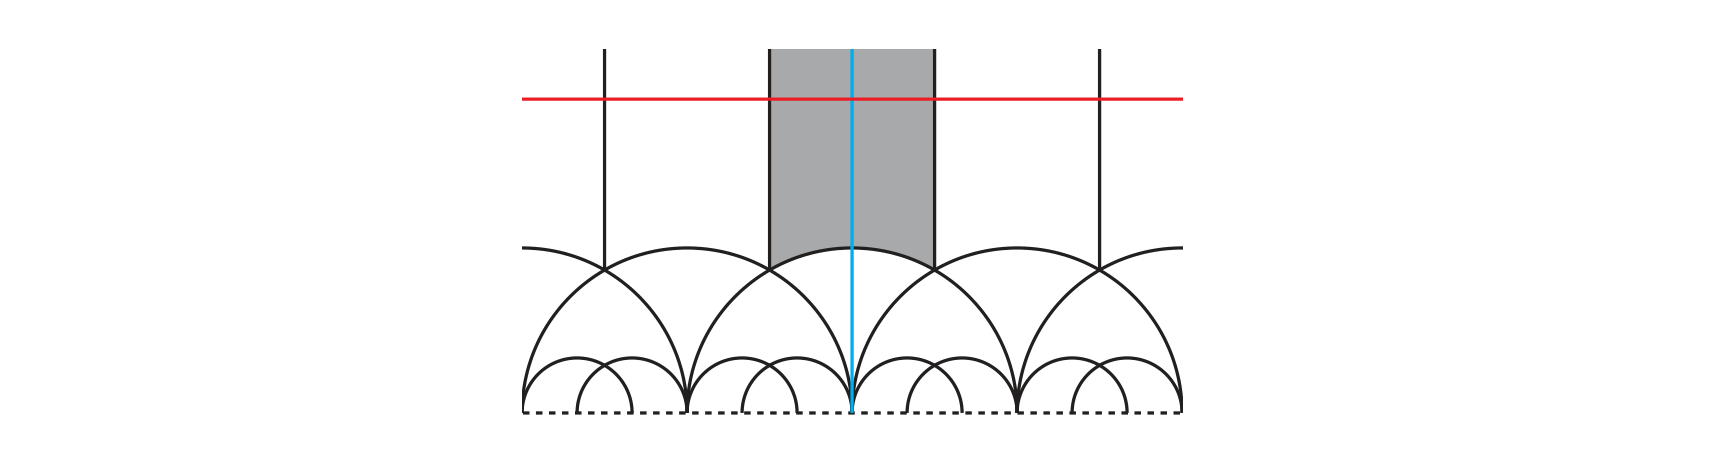
\includegraphics[width=0.6\textwidth]{figure17-1.png}
  \caption{$\mathrm{SL}_2(\Z)$ 作用在 $\mathbb H$ 上的基本域（灰色区域）。
  可以通过对模形式积分（例如沿红线或蓝线）来定义“周期”。
  （原文 p.~293，Figure 17.1）}
  \label{fig:17-1}
\end{figure}

\begin{srcex}{118}
若 $M^{\vee}=T^*X^{\vee}$，则
\begin{equation}\tag{17.96}\label{eq:17.96}
\Loc^{X^{\vee}}_{G^{\vee}}
=\bigl\{\rho\ \text{以及相伴 $X^{\vee}$-丛的平坦截面}\bigr\}.
\end{equation}
有映射
\begin{equation}\tag{17.97}\label{eq:17.97}
\pi\colon\Loc^{X^{\vee}}_{G^{\vee}}\to\Loc_{G^{\vee}},
\end{equation}
于是
\begin{equation}\tag{17.98}\label{eq:17.98}
\cL:=\pi_*\omega.
\end{equation}
我们用 $\omega$ 而不是 $\cO$，原因与我们用 $\IndCoh$ 而不是 $\QC$ 相同。
\end{srcex}

% [Tutor Note: Remark 122 的 “$P_3$-variety” 原文如此（p.291），含义并不标准：按上下文，
%  应是把 $M^{\vee}$ 的 3-移位 Poisson 结构（$P_3$）量子化为 $E_3$-代数；
%  “取上同调”指忘记 $E_3$ 结构只保留交换代数。另 (17.98) 中的 $\omega$ 是 $T^*X^{\vee}$
%  上的全纯体积形式/Canonical bundle 的平方根型对象，之所以用 $\IndCoh$ 是因为
%  $T^*X^{\vee}$ 上自然出现的是（移位）相干层而不是拟凝聚层。]

\section{自守形式的周期（A-侧）}

\begin{sectionkey}
本节从经典数论角度解释 A-侧的边界条件如何产生自守形式的周期：对子群 $H\subset G$ 积分得到
$H$-周期（Eisenstein 周期、Whittaker 周期、Hecke 周期都是特例）；更一般地，球簇 $X$
的周期理论应当由哈密顿 $G$-空间 $M=T^*X$ 的“自守量子化”来理解。
\end{sectionkey}

这种哈密顿辛几何如何从自守侧产生？我们想从经典数论的视角来呈现。

$L$-函数理论中的一个基本问题是：我们怎么知道它可以解析延拓？这在 Galois 侧不是我们能直接
触及的东西。我们谈过一点自守形式的 $L$-函数。把 $L$-函数附着到自守形式有一个直接的想法。
想法是：若 $f$ 是自守形式，则它在除有限多个位之外都非分歧。于是对所有 $p\notin S$ 有 Satake 参数。
这只意味着 Hecke 本征值。Satake 对应的全部要点是：Hecke 本征值对应于
$[F]\in G^{\vee}/G^{\vee}$。对偶群正来源于此。于是我们知道如何附着 $L$-因子：
对 $V\in\Rep(G^{\vee})$ 可以定义
\begin{equation}\tag{17.99}\label{eq:17.99}
L(f,V,s)=\sideset{}{'}\prod_{p\notin S}\frac{1}{\det(1-p^{-s}F_p)}.
\end{equation}

让我们以不同的方式再问这个问题：自守形式上的自然泛函是什么？这是问题“$\mathcal A_G$ 的边界条件
是什么”的特例。要点是：一个边界条件当然会给出 $\mathcal A_G(C)$ 上的泛函，
而 $\mathcal A_G(C)$ 是自守形式空间。让我们转到模形式的图景，故 $G=\mathrm{PSL}_2(\Z)$。
给定特定的闭链，我们可以对模形式积分得到一个数。见图 \ref{fig:17-1}。红线是 horocycle，
将给出 Eisenstein 周期。蓝线将给出 Hecke 周期。$\mathrm{SL}_2\Z$ 上任一模形式 $\varphi$
都有 $q$-展开：
\begin{equation}\tag{17.100}\label{eq:17.100}
\varphi=\sum a_n q^n,
\end{equation}
即它在 $\infty$ 处的 Laurent 展开。于是可以把 $\varphi$ 送到数
\begin{equation}\tag{17.101}\label{eq:17.101}
a_0=\int_{\text{horocycle}}\varphi\,dt.
\end{equation}
这称为 \term{Eisenstein 周期}{Eisenstein period}。（它告诉尖形式与 Eisenstein 级数之间的差别。）
可以把 $y=1$ 写成轨道
\begin{equation}\tag{17.102}\label{eq:17.102}
\int_{y=1}\varphi\,dt=\int_{N(\Z)\backslash N(\R)}\varphi\,dt,
\end{equation}
故这也称为 $N$-周期，其中
\begin{equation}\tag{17.103}\label{eq:17.103}
N=\begin{pmatrix}1&*\\&1\end{pmatrix}.
\end{equation}
系数 $a_1$ 是 Whittaker 周期。

另一个例子，沿蓝线积分，给出 Hecke 周期。即沿虚轴积分：
\begin{equation}\tag{17.104}\label{eq:17.104}
\int_0^{\infty}\varphi(iy)\,\frac{dy}{y}\,y^s.
\end{equation}
可以把它改写为
\begin{equation}\tag{17.105}\label{eq:17.105}
\int_0^{\infty}\varphi(iy)\,\frac{dy}{y}\,y^s=\sum\frac{a_n}{n^s},
\end{equation}
其中 $a_n$ 是 $\varphi$ 的 $q$-展开系数。这是 $\varphi$ 的 $L$-函数：
\begin{equation}\tag{17.106}\label{eq:17.106}
\int_0^{\infty}\varphi(iy)\,\frac{dy}{y}\,y^s
=\sum\frac{a_n}{n^s}=\frac{\Gamma(s)}{(2\pi)^s}L(\varphi,s).
\end{equation}
可以写出
\begin{equation}\tag{17.107}\label{eq:17.107}
L(\varphi,s)=\prod_p\frac{1}{1-a_p p^{-s}+p^{k-1-2s}}.
\end{equation}
当 $\varphi$ 是本征形式时，这恰好是 Hecke 本征值给出的局部 $L$-因子之积。
因子 $\Gamma(s)/(2\pi)^s$ 是 $\infty$ 处的 $L$-因子。

现在我们可能想知道：这与 Galois 侧如何相关？我们怎么知道要做这个积分？定义这个积分需要什么数据？
它与另一侧所需的数据如何相关？更抽象地定义这些周期的方式是：给定子群 $H\subset G$，
可以如下计算 $H$-周期。回忆我们有与 $G$ 相伴的局部对称空间，它是 $\Bun_G$ 的版本：
\begin{equation}\tag{17.108}\label{eq:17.108}
[G]_F=G(F)\backslash G(\mathbb A)/\text{level}.
\end{equation}
在其内部有
\begin{equation}\tag{17.109}\label{eq:17.109}
[H]_F=H(F)\backslash H(\mathbb A)/.
\end{equation}
然后可以定义 $H$-周期为
\begin{equation}\tag{17.110}\label{eq:17.110}
\mathcal{P}_H(\varphi)=\int_{H(F)\backslash H(\mathbb A)}\varphi.
\end{equation}
Eisenstein 周期来自 $H=N\subset\mathrm{PSL}_2$，Hecke 周期来自 $H=T\subset\mathrm{PSL}_2$。

\begin{srcrem}{123}
实际上我们只需要球子群 $H$。这是一个有限性条件，它给出良好的解析性质。
\end{srcrem}

% [Tutor Note: (17.109) 末尾的 “$/\,$” 在原文（p.294）中分母留空，应为与 (17.108) 中
%  “level” 相匹配的级结构（对 $H$ 取同一个 level 的子群）。作者显然省略了它。
%  另 (17.101) 的 horocycle 是 $N(\Z)\backslash N(\R)$（即 $y=1$ 的轨道），其积分给出
%  $q$-展开的常数项 $a_0$；而 $a_1$ 是 Whittaker 周期，对应 $N$-周期取非平凡特征。
%  (17.106) 的推导需要 $\varphi$ 是模形式，且 $a_n$ 按 $q=e^{2\pi i z}$ 展开。]

这来自 Terry Tao 的一篇博客文章。考虑阿贝尔 $L$-函数，即 $G=\mathrm{GL}_1=G^{\vee}$ 的
$L$-函数。例如 Riemann 与 Dedekind $\zeta$-函数是阿贝尔 $L$-函数。还有经典的 Dirichlet
$L$-函数，以及 Hecke 的推广。它们对应于 $\Gal(\overline F/F)$ 的特征。由类域论我们知道，
它们对应于 idèle 类群的特征 $\chi$：
\begin{equation}\tag{17.111}\label{eq:17.111}
\mathrm{GL}_1(F)\backslash\mathrm{GL}_1(\mathbb A).
\end{equation}
这些有时称为 \term{Hecke 本征特征}{Hecke grössencharacters}。

Riemann 把 $\zeta$-函数写成了积分。特别地，$\Xi$ 函数
\begin{equation}\tag{17.112}\label{eq:17.112}
\Xi(s)=\frac{\Gamma(s/2)}{\pi^{s/2}}\xi(s),
\end{equation}
其中可把前因子看作 $\infty$ 处的局部因子，可以写成
\begin{equation}\tag{17.113}\label{eq:17.113}
\Xi(s)=\int_0^{\infty}y^{s/2}\sum_{n=1}^{\infty}e^{-n^2\pi y}\,dy.
\end{equation}
即这是 $\theta$-函数的 Mellin 变换。

局部地（固定有限素数 $p$），在位 $v=p$ 有（局部类域论）
\begin{equation}\tag{17.114}\label{eq:17.114}
K_v^{\times}/\cO_v^{\times}\simeq\Z.
\end{equation}
例如 $\Q_p^{\times}/\Z_p^{\times}\simeq\Z$。在其中我们有
$\varpi\in K_v^{\times}/\cO_v^{\times}$，它对应 $1\in\Z$，即
$p\in\Q_p^{\times}/\Z_p^{\times}$。考虑非分歧局部特征
\begin{equation}\tag{17.115}\label{eq:17.115}
\chi_v\colon K_v^{\times}/\cO_v^{\times}\to\C^{\times}.
\end{equation}
它由单个数确定，即 $\chi_v\in\C^{\times}$。这对应于 $F_v$ 以 $\chi_v$ 作用的
一维 Galois 表示。关键观察：这个特征在 $0$ 处的 $L$-值是
\begin{equation}\tag{17.116}\label{eq:17.116}
L(\chi_v,0)=\frac{1}{1-\chi_v}
=\operatorname{Tr}(\chi_v,\operatorname{Sym}^{\bullet}\C)
=\sum_{n\ge 0}\chi_v^n.
\end{equation}
要点是我们可以把它改写为 $K^{\times}/\cO^{\times}$ 上的积分。特别地可以写
\begin{align}
L(\chi_v,0)&=\frac{1}{1-\chi_v}
=\operatorname{Tr}(\chi_v,\operatorname{Sym}^{\bullet}\C)\tag{17.117}\label{eq:17.117}\\
&=\sum_{n\ge 0}\chi_v^n\tag{17.118}\label{eq:17.118}\\
&=\sum_{n=0}^{\infty}\chi_v\bigl(\varpi^n\in K^{\times}/\cO^{\times}\bigr)\tag{17.119}\label{eq:17.119}\\
&=\int_{K_v^{\times}}\chi_v(x)\cdot1_{\cO_v}\,d^*x.\tag{17.120}\label{eq:17.120}
\end{align}
关键观察是，这个特征函数是\term{局部基本函数}{local basic function}：
\begin{equation}\tag{17.121}\label{eq:17.121}
\Phi_v=1_{\cO_v}.
\end{equation}
$L$-因子可以写成
\begin{equation}\tag{17.122}\label{eq:17.122}
L_v(\chi_v,s)=\int_{K_v^{\times}}\chi_v\Phi_v(x)\,d^*x\cdot|x|_v^s.
\end{equation}
这是 $\Phi_v=1_{\cO}$ 的 Mellin 变换。

让我们退一步。我们在做 $\mathbb G_m\curvearrowright\mathbb A^1$ 的 Fourier 理论。
想 $\mathbb A^1\simeq K\simeq\Q_p$。在其中 $1_{\Z_p}=1_{\cO}$，我们想按
$\mathbb G_m$-作用分解它。$\Phi_v=1_{\cO_v}=1_{\Z_p\subset\Q_p}$ 的实版本是 Gaussian：
\begin{equation}\tag{17.123}\label{eq:17.123}
\Phi_{\infty}(x)=e^{-\pi x^2},
\end{equation}
而 $\infty$ 处的局部 $L$-因子是
\begin{equation}\tag{17.124}\label{eq:17.124}
L_{\infty}=\int_{\R^{\times}}\Phi_{\infty}(x)e^{-\pi x^2}.
\end{equation}

\subsection{Iwasawa--Tate}

\begin{sectionkey}
本小节把特征 $\chi$ 的 $L$-函数写成阿黛尔空间上的积分（Iwasawa--Tate 公式）：
它是对 $\theta$-级数求和后用 $\chi$ 配对，本质上是 $K^\times/\cO^\times\simeq\Z$ 上的
Fourier/Pontrjagin 对偶；在函数域情形这给出几何版本的 $\Theta=\pi_*1$。
\end{sectionkey}

可以把特征的 $L$-函数改写为
\begin{equation}\tag{17.125}\label{eq:17.125}
L(\chi,s)=\int_{F^{\times}\backslash\mathrm{GL}_1(\mathbb A)}
\chi(x)\cdot\sum_{\gamma\in F}\Phi(\gamma x)\,d^*x,
\end{equation}
其中
\begin{equation}\tag{17.126}\label{eq:17.126}
\Phi=\prod_v\Phi_v.
\end{equation}
这是
\begin{equation}\tag{17.127}\label{eq:17.127}
\sideset{}{'}\prod_{F_v}\mathbb A^1_{F_v}
\end{equation}
上的函数。这是对（比如）$\Q$ 的求和，那么它与之前对 $\Z$ 的求和如何相关？嗯：
\begin{equation}\tag{17.128}\label{eq:17.128}
\sum_{\gamma\in F}\Phi(\gamma\cdot x)=\sum_{\gamma\in\cO_F}\Phi_{\infty}(\gamma x),
\end{equation}
即我们得到 $x$ 的平移上的 Gaussian 之和。这就是 $\theta$-级数。有算子
\begin{equation}\tag{17.129}\label{eq:17.129}
\Theta\colon\operatorname{Fun}\bigl(\mathbb A^1_{\mathbb A}\bigr)
\to\operatorname{Fun}\bigl([\mathrm{GL}_1]\bigr),
\end{equation}
它由对所有平移求和给出：
\begin{equation}\tag{17.130}\label{eq:17.130}
\Theta(\Phi)=\sum_{\gamma\in F}\Phi(\gamma\cdot x).
\end{equation}
注意 $\Phi\in\operatorname{Fun}(\mathbb A^1_{\mathbb A})$，事实上
\begin{equation}\tag{17.131}\label{eq:17.131}
L(\chi)=\int\chi\Theta(\Phi)=\langle\chi,\Theta\rangle.
\end{equation}

在函数域情形我们有
\begin{equation}\tag{17.132}\label{eq:17.132}
\operatorname{Pic}(C)(k)=F^{\times}\backslash\mathbb A^{\times}\big/\mathbb A_A^{\times}.
\end{equation}
则
\begin{equation}\tag{17.133}\label{eq:17.133}
\Theta_{\Phi}\colon\operatorname{Pic}\ni L\mapsto
\sum_{\gamma\in F^{\times}}\Phi(\gamma\cdot L)=\# H^0(C,L).
\end{equation}
几何地，
\begin{equation}\tag{17.134}\label{eq:17.134}
\begin{array}{ccc}
\operatorname{Pic}^{\mathbb A^1} & = & \text{线丛及相伴 $\mathbb A^1$-丛的截面}\\[2pt]
\downarrow{\scriptstyle \pi} & & \\[2pt]
\operatorname{Pic} & = & \text{线丛}
\end{array}
\end{equation}
且
\begin{equation}\tag{17.135}\label{eq:17.135}
\Theta=\pi_*1.
\end{equation}
现在我们可以非常容易地把它推广到非阿贝尔群。

% [Tutor Note: (17.116)--(17.120) 的关键是把 $\Z$ 上的几何级数 $\sum\chi_v^n$ 写成
%  $K_v^\times$ 上的积分：$\varpi^n$ 对应 $n\in\Z$，而 $1_{\cO_v}$ 是“基本函数”。
%  这正是 Iwasawa--Tate 理论的核心：$L$-因子是局部基本函数的 Mellin 变换。
%  (17.128) 中求和从 $\gamma\in F$ 换成 $\gamma\in\cO_F$，原因是 $\Phi_\infty$ 为 Gaussian
%  而其余 $\Phi_v=1_{\cO_v}$ 只在整点上非零（对 $F=\Q$ 时 $\cO_F=\Z$）；这一步是
%  Poisson 求和/函数方程的技术核心，作者未展开。]

\section{一般版本}

\begin{sectionkey}
本节把周期理论推广到任意球簇 $G\curvearrowright X$：周期 $P_X$ 由 $\Bun^X_G\to\Bun_G$
的推出给出，而对偶侧由哈密顿 $G^{\vee}$-空间 $M^{\vee}$ 与 Plancherel 测度刻画；
由此陈述三个猜想（整体数值、整体几何、局部几何），把周期与 $L$-函数、Plancherel 测度与
$\Shv(X(K)/G(\cO))$ 的 Satake 对应联系起来。
\end{sectionkey}

起点数据是群作用在簇上：$G\curvearrowright X$。

\begin{srcex}{119}
取 $G\curvearrowright G/H$、$\mathrm{PSL}_2\curvearrowright\mathrm{PSL}_2/T$ 以及
$\mathrm{GL}_1\curvearrowright\mathbb A^1$，就还原到我们之前考虑的具体情形。
\end{srcex}

现在我们有
\begin{equation}\tag{17.136}\label{eq:17.136}
\sideset{}{'}\prod X(K)/G(\cO)=\Bun^X_G=\operatorname{Map}(C,X/G),
\end{equation}
它由带 $X$-丛截面的 $G$-丛组成。有投影映射
\begin{equation}\tag{17.137}\label{eq:17.137}
\begin{array}{ccc}
\sideset{}{'}\prod X(K)/G(\cO) & \Bun^X_G & \operatorname{Map}(C,X/G)\\[2pt]
\downarrow{\scriptstyle\pi} & \downarrow{\scriptstyle\pi}
& \downarrow{\scriptstyle\pi}\\[2pt]
G(F)\backslash G(\mathbb A)/G(\cO_{\mathbb A}) & \Bun_G
& \operatorname{Map}(C,\mathrm{pt}/G)
\end{array}
\end{equation}

\begin{srcex}{120}
若 $X=G/H$，则 $\Bun^X_G=\Bun_H$。
\end{srcex}

于是现在有自然映射。自守形式的 $X$-周期就是
\begin{equation}\tag{17.138}\label{eq:17.138}
\mathcal{P}_X(\varphi)=\langle\Theta_X,\varphi\rangle_{\Bun_G},
\end{equation}
其中
\begin{equation}\tag{17.139}\label{eq:17.139}
\Theta_X=\pi_*1.
\end{equation}
或者由伴随可以写
\begin{equation}\tag{17.140}\label{eq:17.140}
\mathcal{P}_X(\varphi)=\langle\Theta_X,\varphi\rangle_{\Bun_G}
=\int_{\Bun^X_G}\pi^*\varphi.
\end{equation}

我们在忽略这些积分与求和的收敛性问题。需要知道一些解析性质，它们将来自对 $X$ 的强有限性假设。
这就是球簇理论登场之处。

Ben-Zvi--Sakellaridis--Venkatesh 即将开展的工作的要点如下。设 $G\curvearrowright X$ 是球性的。
这定义了自守理论 $\mathcal A_G$ 的边界条件。要点是：周期理论是边界数据理论的三维部分。
但从物理上说，我们应该使用哈密顿 $G$-空间，而不只是 $G$-空间。由 $G\curvearrowright X$ 的数据，
得到哈密顿 $G$-空间 $M=T^*X\circlearrowleft G$。断言是：周期理论是\term{微局部}{microlocal}的。
即它真正是关于 $M$（而不是 $X$）的“自守量子化”。在 Tate 的论文中，关键要素是函数方程来自
在 $\mathbb A^1$ 上做 Fourier 变换。但 Fourier 变换不是 $\mathbb A^1$ 的对称性，而是
$T^*\mathbb A^1$ 由 90 度旋转给出的对称性。$L$-函数不依赖 $\mathbb A^1$ 而依赖
$T^*\mathbb A^1$ 这一事实，意味着它在此对称性下不变，从而特别地在 Fourier 变换下不变，
这就给出函数方程。

事实上有很多与 $G\curvearrowright M$ 相伴的周期例子，其中 $M$ 不是余切丛。例如 Whittaker
周期 $a_1$ 自然地来自一个\term{扭余切丛}{twisted cotangent bundle}。还有所谓
\term{theta 对应}{theta correspondence}，它来自研究不是余切丛的辛空间。这些一般来自一般辛表示
$G\curvearrowright V$，它可能不是 $W\oplus W^*$。故这是周期的一个重要来源。

\begin{srcrem}{124}
如上所述，使所有这些积分收敛所需的有限性来自 $X$ 是球性的。对 $M$ 的类似条件是什么？
我们坚持要求 $\cO(M)^G$ 是 Poisson 交换的。这些称为\term{重数 1 哈密顿空间}{multiplicity 1
Hamiltonian space}。超球性（hyperspherical）则是此条件再加几条额外条件。
\end{srcrem}

这个名字的动机来自 hypertoric 簇。这个名字来自它们是超 Kähler 的。

% [Tutor Note: Remark 124 的末两句在原文（p.297）中指代混乱：“The name is motivated by
%  hypertoric varieties. This name comes from them being hyperkähler.”——两个 “name” 指的
%  应是不同的东西（“multiplicity 1” 的命名动机与 “hypertoric” 的词源）。按数学含义，
%  hypertoric 簇是“超 Kähler 的环面簇”，其名称来自 hyperkähler + toric；
%  而“重数 1”指的是 $\cO(M)^G$ 在 Poisson 交换意义下的重数。这里照原文译出并提示。]

BZ-Sakellaridis-Venkatesh 的想法是用边界条件理论来组织周期理论。于是自守侧的周期在 B-侧
将有对偶。这有点模糊，但由此我们可以用重构提取对偶群的哈密顿簇：
\begin{equation}\tag{17.141}\label{eq:17.141}
G^{\vee}\curvearrowright M^{\vee}.
\end{equation}
我们说过 $G^{\vee}\curvearrowright M^{\vee}$ 与 $L$-函数相关，而 $G\curvearrowright M$
与周期相关。故这建立了周期与 $L$-函数之间的桥梁。

\begin{srcconj}{3}（整体数值/算术）
自守形式的 $X$-周期的范数由相应的 $L$-函数给出：
\begin{equation}\tag{17.142}\label{eq:17.142}
|\mathcal{P}_X(\varphi)|^2=L(\rho,M^{\vee}),
\end{equation}
其中 $\varphi$ 对应于 $\rho\colon\Gal\to G^{\vee}$。
\end{srcconj}

\begin{srcrem}{125}
这里 $|\cdot|^2$ 来自如下事实：这秘密地是关于 $M=T^*X$ 而不只是 $X$ 的。
\end{srcrem}

现在可以到处跑并做出大量猜想。

\begin{srcconj}{4}（整体几何）
回忆我们有
\begin{equation}\tag{17.143}\label{eq:17.143}
\cL_{M^{\vee}}\in\QC^{!}\bigl(\Loc_{G^{\vee}}\bigr)=\mathcal B_{G^{\vee}}(C),
\end{equation}
由沿
\begin{equation}\tag{17.144}\label{eq:17.144}
\Loc^{X^{\vee}}_{G^{\vee}}\to\Loc_{G^{\vee}}
\end{equation}
的前推给出。我们可以在 A-侧做同样的事情。我们有
\begin{equation}\tag{17.145}\label{eq:17.145}
\mathcal A_G(C)=\Shv\bigl(\Bun_G(C)\bigr).
\end{equation}
在其内部得到周期层，即
\begin{equation}\tag{17.146}\label{eq:17.146}
\mathcal{P}_X=\pi_*k,
\end{equation}
其中
\begin{equation}\tag{17.147}\label{eq:17.147}
\pi\colon\Bun^X_G\to\Bun_G.
\end{equation}
\end{srcconj}

$M^{\vee}$ 从自守形式的观点看是什么意思？在自守侧，Sakellaridis--Venkatesh 写了 [SV17]，
其中研究整体周期理论与表示论（调和分析）中局部问题之间的关系。

对局部域上的 $G$-簇该做什么？首先考虑局部算术情形。于是可以考虑 $X$ 在 $K$ 上的函数空间
$X(K)$。群 $G(K)$ 作用在其上，故可以（比如）把 $L^2(X(K))$ 分解为 $G(K)$ 的表示。
这正是局部 Langlands 对应中出现的那类对象。

不那么贪心的做法是看球函数的概念。这意味着考虑 $X(K)$ 上在 $G(\cO)$ 的正半部分下不变的函数。
这现在是 Hecke 代数的一个表示：
\begin{equation}\tag{17.148}\label{eq:17.148}
X(K)/X(\cO)\curvearrowright k\bigl[G(\cO)\backslash G(K)/G(\cO)\bigr]
\simeq\bigl|\Rep(G^{\vee})\bigr|.
\end{equation}
% [Tutor Note: 原文 p.298 的 "the positive half of $G(\cO)$" 一语，作者在本书中未另作定义；
%  按 (17.149) 的语境，它指 $G(\cO)$ 里相对 Iwahori 子群的正向部分，"在该部分下不变"
%  应读作相应的 Iwahori 不变条件，而与 "$G(\cO)$ 本身分正负半" 无关。
%  [译者按（无外部依据）：仅据 (17.149) 上下文与 Iwahori 分解的通行约定读出。]]
$X$ 是球簇，等价于 $G(\cO)\curvearrowright X(K)$ 有离散轨道。例如仿射 Grassmann 簇。

于是现在考虑 Hecke 代数作用在球函数上：
\begin{equation}\tag{17.149}\label{eq:17.149}
\cH\simeq\bigl|\Rep(G^{\vee})\bigr|\curvearrowright L^2\bigl(X(K)/G(\cO)\bigr).
\end{equation}
$\Phi=1_{X(\cO)}$ 是球函数。$\Theta$ 算子是
\begin{equation}\tag{17.150}\label{eq:17.150}
\Theta\colon\sideset{}{'}\bigotimes L^2\bigl(X(K)/G(\cO)\bigr)\to L^2(\Bun_G),
\end{equation}
且
\begin{equation}\tag{17.151}\label{eq:17.151}
\Theta(\Phi)=\mathcal{P}_X.
\end{equation}

% [Tutor Note: (17.148) 左端的 $X(K)/X(\cO)$ 在原文（p.298）中如此印出，但按上下文
%  （球函数是 $X(K)$ 上 $G(\cO)$-不变的函数）这里应为 $X(K)/G(\cO)$，即
%  “$G(\cO)$ 作用在 $X(K)$ 上”。分母写成 $X(\cO)$ 是原文笔误（也可能是把
%  商 $X(K)/G(\cO)$ 与 $X(\cO)$ 的记号混用）。这里照原文保留并在 (17.148) 中提示；
%  (17.149) 起即改用正确的 $X(K)/G(\cO)$。]

所以我们想理解 $L^2(X(K))$ 的 Plancherel 测度。这是 $G(K)$ 的酉表示集合上的测度。
由局部 Langlands 对应，它与局部 Langlands 参数相匹配。代替它，我们可以考虑球函数并尝试按
$\cH$-作用分解。回忆
\begin{equation}\tag{17.152}\label{eq:17.152}
\cH\simeq\bigl|\Rep(G^{\vee})\bigr|\simeq\cO\bigl(G^{\vee}/G^{\vee}\bigr).
\end{equation}

我们甚至不会尝试分解整个空间。只看这个基本函数 $\Phi$。

所以我们问的是调和分析问题，而我们将几何地回答它。给定 Hilbert 空间中的一个状态 $\Phi$，
从中得到的是算子代数谱上的一个谱测度。在我们的情形，我们编码包含 $\Phi$ 的 $\cH$-作用的
轨道的所有不同乘积，即
\begin{equation}\tag{17.153}\label{eq:17.153}
\langle H_v\cdot\Phi,H_w\cdot\Phi\rangle
\end{equation}
其中 $H_v,H_w\in\cH\simeq|\Rep(G^{\vee})|$。这决定了 Hecke 代数谱上的测度，
即 Plancherel 测度。这告诉我们 $\Phi$ 如何分解，因为 $\cH\simeq|\Rep(G^{\vee})|$。
事实上，同一个表示控制了 $X$-周期理论中出现的整体 $L$-函数。“（对 $X$ 的）周期的平方”
看起来就像 $X$ 的 Plancherel 测度的 Euler 积。

如何几何地思考这一点？这将解释对偶边界条件从何而来。要点是
$M^{\vee}\circlearrowleft G^{\vee}$ 是 $X(K)/G(\cO)$ 的 Plancherel 测度的范畴化形式。

同一个问题的几何版本如下。我们用层替换函数：
\begin{equation}\tag{17.154}\label{eq:17.154}
\Shv\bigl(X(K)/G(\cO)\bigr).
\end{equation}

\begin{srcex}{121}
若 $X=G$ 且 $G\times G\curvearrowright G$，则这还原仿射 Grassmann 簇
$G(\cO)\backslash G(K)/G(\cO)$。
\end{srcex}

球性条件模仿了这个例子的离散方面。在其中有一个基本层：
\begin{equation}\tag{17.155}\label{eq:17.155}
\Phi=k_{X(\cO)}\in\Shv\bigl(X(K)/G(\cO)\bigr).
\end{equation}
即我们用常值层替换特征函数。

那 Plancherel 测度呢？可以几何地做同样的事情。用 $\Hom$ 替换配对，于是考虑
\begin{equation}\tag{17.156}\label{eq:17.156}
\Hom_{\Shv}\bigl(H_V*\Phi,H_W*\Phi\bigr).
\end{equation}
这个空间上的 Frobenius 迹将给我们经典调和分析。这一切都由单个对象捕获，
即 Plancherel 测度的类似物：它由
\begin{equation}\tag{17.157}\label{eq:17.157}
\cA_X=\End_{\cH}(\Phi)
\end{equation}
捕获，这里是内 Hom，即有函子
\begin{equation}\tag{17.158}\label{eq:17.158}
\cH\to\Shv\bigl(X(K)/G(\cO)\bigr),
\end{equation}
由作用在 $\Phi$ 上给出。有一个伴随，由 $\Hom(\Phi,-)$ 给出。即 $\cA$ 是
\begin{equation}\tag{17.159}\label{eq:17.159}
\cH=\Shv\bigl(G(\cO)\backslash G(K)/G(\cO)\bigr)=\mathcal A_G(S^2)
\end{equation}
中的代数对象。

它不只是某个旧代数对象，事实上它是结合的因子化代数。即它是
$\mathcal A_G(S^2)$ 中 $E_3$-代数对象的某种版本。但这正是我们出发时的数据：
从边界条件出发，我们（除其他东西外）找到了线算子中的一个代数。当我们仔细思考在局部情形
得到什么时，$\cA_X$ 恰好是边界条件上局部算子的代数。于是对偶哈密顿空间是
\begin{equation}\tag{17.160}\label{eq:17.160}
M^{\vee}=\Spec_{/(\mathfrak g^{\vee*}/G^{\vee})}(\cA_X)
\in\mathcal A_G(S^2),
\end{equation}
并回忆
\begin{equation}\tag{17.161}\label{eq:17.161}
\mathcal A_G(S^2)=\mathcal B_{G^{\vee}}(S^2)
=\QC\bigl(\mathfrak g^{\vee*}/G^{\vee}\bigr),
\end{equation}
即 $M^{\vee}$ 是 Plancherel 测度支撑的几何版本。矩映射的支撑就是 Plancherel 测度的支撑。

Sakellaridis、Sakellaridis--Venkatesh 以及 Sakellaridis--Wang 计算了大量关于 Plancherel
测度的内容（原文此处标注 cite$^3$）。于是我们可以精确描述 $M^{\vee}$。然后可以陈述一些猜想。
其中最基本的一条如下。

\begin{srcconj}{5}（局部几何）
边界上的线算子相匹配：
\begin{equation}\tag{17.162}\label{eq:17.162}
\Shv\bigl(X(K)/G(\cO)\bigr)\simeq\QC\bigl(M^{\vee}/G^{\vee}\bigr),
\end{equation}
且与如下作用相容：
\begin{equation}\tag{17.163}\label{eq:17.163}
\cH\simeq\QC\bigl(\mathfrak g^{\vee*}/G^{\vee}\bigr).
\end{equation}
（注：后一个同构是 Satake。）
\end{srcconj}

% [Tutor Note: (17.148) 与 (17.152) 中的 $|\Rep(G^{\vee})|$ 记号并不标准：作者用它表示
%  “Hecke 代数所对应的范畴/代数”，即 Satake 等价 $k[G(\cO)\backslash G(K)/G(\cO)]
%  \simeq\Rep(G^{\vee})$ 的（导出）版本；竖线可能表示取“底层范畴”或“同伦范畴”。
%  阅读时把它当作 Satake 等价的简写即可。(17.159)--(17.161) 则说明：边界条件的线算子范畴
%  $\mathcal A_G(S^2)$ 同构于 $\QC(\mathfrak g^{\vee*}/G^{\vee})$，而 $M^{\vee}$ 相对谱
%  正是 Plancherel 测度支撑的几何化；(17.162) 把 Plancherel 测度的支撑与
%  $\Shv(X(K)/G(\cO))$ 的谱联系起来。最后，Conjecture 3、4、5 分别对应数值（周期范数）、
%  整体几何（$L$-层与周期层）、局部几何（Plancherel 测度）三个层次。]


% ---------------------------------------------------------------------------
% 附录
% ---------------------------------------------------------------------------
\appendix
% ============================================================================
%  附录：审校批注汇编（由 % [Tutor Note: ...] 自动汇编，纯文本呈现）
% ============================================================================
\chapter{审校批注汇编}\label{app:notes}

\begin{quote}
\small
本附录把全书正文中以 \texttt{\% [Tutor Note: ...]} 形式就近标注的译者批注集中列出，
按章、节顺序排列，便于单独查阅。批注分四类：易错预警、作者省略的证明、原文校勘、
物理图像说明。批注只代表译者的核对意见，不改变正文。为保证本附录在任何 TeX 环境下
都能编译，此处以纯文本呈现公式片段；完整 LaTeX 形式见各章源码中的注释。
\end{quote}

\section{概述}
\subsection*{模形式/自守形式 / 粗略想法}
\begin{quote}\small
式 (1.5) 中的 $\omega$k/2 在 k 为奇数时并不是通常意义下的线丛（需要 spin 结构， 或按自守因子的半整数权来理解）。作者在这里把“模形式 = 典范丛幂次的全纯截面”一笔带过， 严格处理需要引入覆盖群 Mp2(R) 或 metaplectic 结构；这是后续讨论半整数权模形式时的常见陷阱。
\end{quote}

\subsection*{模形式/自守形式 / 结构}
\begin{quote}\small
式 (1.8) 只是“换基域”的隐喻性图示，并不是说 OF 等于 Z 作基变换。 正确的陈述是：OF 是 F 在 Q 上的整闭包；对 F/Q 有限，F 是 SpecZ 上的有限平坦覆盖 （在分歧素点处退化）。把它读成“base change”会误导后续对分歧的几何理解。
\end{quote}

\begin{quote}\small
式 (1.11) 中的记号 R$\times$ r1 表示 r1 个 R 的直积，C$\times$ r2 同理； 这里 $\times$ 是“笛卡尔积”而非群乘法。对 F=Q(d) 可直接验证：实二次域给出两个实嵌入， 虚二次域给出一个共轭对。后续计算 MG,F 的维数/体积时，这个分解是第一道易错关口。
\end{quote}

\subsection*{Langlands 纲领与 TFT / 概览}
\begin{quote}\small
式 (1.20) 中的 GC 指 Langlands 对偶群的 C-点，通常写作 G(C)。 这里 G 是 Q 上的约化群，G 是其复对偶群；而 Gal(F/F) 是绝对 Galois 群。 对 G=GLn，G=GLn(C)，这正是通常的 n 维 Galois 表示。对一般 G， “G-值表示”需要把 Galois 表示与对偶群的中心/连通分量问题一起考虑。
\end{quote}

\begin{quote}\small
式 (1.22) 的物理来源是 Kapustin–Witten 对 4d N=4 超对称 Yang–Mills 的 S-对偶作拓扑扭转；A-侧对应自守/磁侧，B-侧对应谱/电侧。它不是已证明的定理， 而是组织猜想的原则。这里作者用“等价”一词，读者应理解为“conjectural equivalence of TFTs”；严格陈述需要指明边界条件、算子与范畴的层级。
\end{quote}

\subsection*{Langlands 纲领与 TFT / 算术拓扑}
\begin{quote}\small
原书此表“圆盘”一行印作 SpecFt[[t]]（见 p.15），从上下文看应为 SpecFq[[t]]：q 是基域 Fq 的基数，t 是形式参数。这属于原稿笔误，译文按数学上正确的 Fq[[t]] 处理；若读者对照原 PDF 会发现此差异，特此说明。
\end{quote}

\begin{quote}\small
式 (1.27)–(1.29) 描述的是局部域绝对 Galois 群的驯分歧商： 惯性群 Iv 的驯部分同构于 $\prod$$\ell$'$\neq$ pZ$\ell$'(1)，而野惯性群是 pro-p 群； 商 Z$\ell$Z 中的 Z$\ell$ 来自 $\ell$-进循环（$\ell$$\neq$ p），Z 由 Frobenius 生成。 原文在 (1.29) 前有一句残句 “This tells us that there is For p=1, ...”， 其中 “there is” 之后的文字被截断/错位；“p=1” 与 “p=-1” 也不是素数， 而是 Baumslag–Solitar 群的退化参数。译文按 BS(1,1)=Z²、BS(1,-1)=Klein 瓶的基本群处理， 并保留原文的表述方式。
\end{quote}

\subsection*{Langlands 纲领与 TFT / $\mathcal{B}$-侧}
\begin{quote}\small
原文此处印作 “The B-wide is about studying...”，其中 “B-wide” 显然是 “B-side” 的笔误（p.19）。译文按 B-side 处理。
\end{quote}

\section{谱分解}
\subsection*{什么是谱？}
\begin{quote}\small
这里伴随的方向容易记反。O 是反变函子，故其“右伴随”应理解为在 Ringop 与 Spacesop 上的左伴随；若忘记取 op，就会把 Spec 误认为左伴随。正确读法是：Spec,R 表示“以 R 为函数环的自由空间”，而 (2.1) 表明这种自由性对一切测试空间成立。另注意 MapSpaces 必须理解为 plain hom-set（0-截断），否则伴随性只在同伦意义下成立。
\end{quote}

\subsection*{什么是谱？ / 紧支撑连续函数}
\begin{quote}\small
记号 Cv(X) 并非通用记号，通常写作 C0(X)（contract 支撑/消失于无穷）。若 X 非紧，C0(X) 不含单位元，此时应在单位化代数 C0(X)+ 上取极大理想，或改用“本原理想/特征”，否则 (2.4) 的 HomC*(A,C) 会漏掉零同态之外的信息。作者在正文中默认的应是“含单位的交换 C*-代数”与紧 Hausdorff 空间，非紧情形要靠单位化补救；这是引用 Gelfand--Naimark 时最常见的隐藏约定。
\end{quote}

\subsection*{什么是谱？ / 代数几何}
\begin{quote}\small
(2.8) 的交换图应读成：Spec: cRingop 与“整体截面”函子 $\Gamma$ 的伴随关系在仿射对象上的像；竖箭头表示“仿射概形 $\hookrightarrow$ 局部环空间”的满子范畴包含。作者用图把 Spec 画成从 cRing 指向仿射概形，实际方向是反变的，读图时须注意箭头两端是范畴而非函子。
\end{quote}

\subsection*{谱分解}
\begin{quote}\small
印刷版 (2.14) 末尾多出一个 w，从上下文看是排版残留（应与 (2.11) 中带下划线的 V 记号无关，也不进入任何公式）。照录于此；正确写法应为 V=$\lambda$$\in$ XV$\lambda$。另注意 (2.12) 的支撑本应定义为 Spec,R 中的闭子集而非 X，此处 X 是作者对“底空间”的泛称；在有限集情形二者一致，但一般 R 上应说 Supp(v)$\subset$Spec,R。
\end{quote}

\subsection*{谱定理 / 代数几何版本}
\begin{quote}\small
(2.21) 用并集而非直和，是因为不同 $\lambda$ 上的支撑集合可能相交于 0（即同时在两处支撑的向量只能为 0）；对有限生成模，实际只有有限多个 $\lambda$ 使 V$\lambda$$\neq$ 0，所以该并是有限并、无收敛问题。(2.24) 的下标写成 $\lambda$$\in$Spec 是省略了 Spec,k[x]=A1；$\lambda$ 表示“以 $\lambda$ 为中心的广义特征空间”，即 (2.25) 中的 k[x]/(x-$\lambda$)$\ell$i 部分，注意它与 (2.16) 的 V$\lambda$（真特征空间）不同：后者是前者的商。
\end{quote}

\subsection*{谱定理 / 可测版本}
\begin{quote}\small
(2.32) 左右两端用同一字母 $\pi$A 表示两个不同对象：左边带下划线的是层 $\pi$A，右边是投影算子值测度（对可测集取投影算子）。这种“同一符号、两种范畴”的写法是本节最容易混淆处。另注意 (2.31) 的积分只在 A 自伴时才是实轴上的谱积分；若 A 非自伴（或非正规），应改在 C 上取谱测度，且 (2.34) 的 Spec(A) 不再自动是实子集。
\end{quote}

\subsection*{谱定理 / 同伦版本}
\begin{quote}\small
印刷版 (2.39) 右端写作 C*(X)，但若如此则右边恒等于 M，与开集 U 无关，不可能定义出层。正确形式应是 M(U)=M$\otimes$C*(X)C*(U)：用 U 上的上链把常数模 M “局部化”。这里照录原文并加校勘；读者可按修正后的公式理解后面的陈述。(2.35) 的嵌入也不是逐点单射，而是在拟同构意义下把 R-模视为 X 上的局部常值复形。
\end{quote}

\subsection*{谱定理 / 物理诠释：可观测量与态}
\begin{quote}\small
印刷版 (2.43) 右端明显有误：|$\psi$i$\rangle$ 是未配对的右矢，且与左端（正数）量纲不符；按 Jordan 谱分解应写成 (1)/($\langle$|$\rangle$)$\Sigma$$\lambda$,$\psi$i$\lambda$,$\langle$$\psi$i|$\rangle$$\langle$|$\psi$i$\rangle$，即 $\lambda$|$\langle$$\psi$i|$\rangle$|2。这里照录原文并标出。另注意 (2.42) 的期望值用 $\langle$|$\rangle$ 归一化，与通常“态已归一化”的约定不同；作者在全书中保持这一不归一化的约定，在后续出现 $\rangle$ 的地方须与此一致。
\end{quote}

\section{Fourier 理论与阿贝尔对偶}
\subsection*{特征标}
\begin{quote}\small
印刷版 (3.2) 写作 Aut(X)，但按上下文（g$\mapsto$ Tg 是 V 上的算子、且右侧为 End(V)）应为 Aut(V)。这是原文笔误，照录并标出。另注意 Aut(V)$\subset$End(V) 只是幺半群包含：G 的群同态经此包含成为到乘法幺半群的映射，这正是下一节 (3.6)--(3.8) 要用“幺半群而非群”作伴随的原因。
\end{quote}

\subsection*{有限 Fourier 变换}
\begin{quote}\small
当 G 非交换时 C G 非交换，Spec 无从谈起；因此本章最终必须限制到 Abel 群（作者随后即如此假设）。(3.10) 把 C G 写成“函数之和”，实际只在 G 有限时成立；一般 G 应写成有限支撑函数（即测度）的代数，这就是正文紧接着强调“应把 f 想成测度”的原因。
\end{quote}

\begin{quote}\small
(3.21) 的对偶性要成立必须限制在 Abel 群 G 上；Spec(C G,$\ast$) 中的 $\ast$ 提醒读者这里取的是卷积乘法。另注意 (3.22) 的 g 是指 g 在对偶群中对应的特征标 $\chi$$\mapsto$$\chi$(g)，而不是某个新变量；下一小节 (3.26) 的双对偶映射会把它讲清楚。
\end{quote}

\subsection*{有限 Fourier 变换 / 隐藏的对称性}
\begin{quote}\small
(3.31) 的复共轭不能丢：在有限 Abel 群上 $\chi$(g,t)=$\chi$(g,t)-1，它正是逆变换中“正交关系”的来源，也是 (3.32) 不含共轭的原因。若把 (3.31)(3.32) 视为互逆变换，还必须补上归一化因子 1/|G|（或把 f 视为测度、 f 视为函数），作者在这里用的是“测度--函数”约定，故两式表面上不对称。
\end{quote}

\subsection*{Pontrjagin 对偶}
\begin{quote}\small
对一般 LCA 群，G 要取紧开拓扑才成为拓扑群（Pontrjagin 定理）；(3.34) 只写了集合。“G 紧 $\Leftrightarrow$ G 离散”这一条（见 p. 35）正是紧开拓扑的直接推论，后文 (3.50)--(3.51) 用它解释 e2$\pi$ inx$\in$ L2 与 $\delta$n$\in$$\ell$2 的差别。
\end{quote}

\subsection*{Pontrjagin 对偶 / 群代数}
\begin{quote}\small
印刷版 (3.35) 的被积函数用了自由变量 h，而积分变量是 g，这在原文中即不一致。按 (3.18) 的推前定义应写成 $\int$g$\in$ Gf1(g)f2(g-1h),dg，或把积分变量改为 h。叉积次序（gh-1 还是 g-1h）取决于群乘法约定，翻译时照录原文，读者按 f1$\ast$ f2(h)=$\int$ f1(g)f2(g-1h)dg 校正即可。
\end{quote}

\begin{quote}\small
严格说 L1(G) 只是 Banach *-代数而非 C*-代数（C*-包络才得到群 C*-代数 C*(G)）；作者说“C*-代数世界”是口语化的说法。用 L1(G) 的好处是（对 Abel G）Gelfand 理论直接给出 G，无需先取包络。
\end{quote}

\begin{quote}\small
(3.43) 右端照印本写作 L2(G)，按 Fourier 变换的定义应为 L2(G)（Plancherel 定理：Fourier 变换是 L2(G)$\to$ L2(G) 的等距同构）。这是原文的记号笔误，特此标出。
\end{quote}

\subsection*{Fourier 变换}
\begin{quote}\small
(3.53) 与 (3.54) 的左边都印作 T，但二者说的是不同对象的对偶：环面的对偶是格 $\Lambda$（离散），格的对偶是环面 $\Lambda$$\otimes$ZU(1)。作者用同一个符号 T 是记号滥用；后文 (3.81)(3.124) 中的 T 一律指“对偶环面”。这是阅读本节最容易出错处。
\end{quote}

\begin{quote}\small
(3.63) 印刷版右端为 “SpecRR[d/dx=t]”，其中连续出现两个 R 是排版重复，应读作 SpecRR[d/dx=t]：即在实系数多项式环 R[d/dx] 上取 Spec，得到 Rt。这里 g=R（G=R 的交换 Lie 代数），g*=Rt 是“动量/频率”坐标所在的直线，与 (3.57) 中 t 的角色一致。
\end{quote}

\subsection*{在量子力学中}
\begin{quote}\small
(3.66) 取 pj=i,d/dqj（数学约定，$\hbar$ 已吸收进 p），此时 [pj,qk]=i$\delta$jk；而 (3.67) 又写成 $\xi$ f=f$\xi$+$\hbar$ f'，两式的归一化并不一致——若按 (3.66)，(3.67) 右端应为 i f'（或把 p 改回物理约定 -i$\hbar$$\partial$）。此外 (3.67) 中 f' 应理解为 $\xi$(f)，即沿 $\xi$ 的方向导数，而非对某个坐标的偏导。这是本节最容易混用的符号。
\end{quote}

\subsection*{Cartier 对偶}
\begin{quote}\small
点函子的 R 取遍所有交换环（不只是域），这是“概形论”代数群与“经典”代数群的关键差别：例如 Z 作为代数群只在此意义下才是群概形。(3.72) 中的虚线提升不是自动的，它等价于给定 G(R) 的群结构对 R 函子化；作者略去的“群运算与结构态射相容”条件通常还要求乘法、单位、逆都是簇态射。
\end{quote}

\begin{quote}\small
(3.85) 的并集写成 nSpec,k[t]/(tn) 是（形式）归纳极限而非普通概形：每个 Spec,k[t]/(tn) 是加厚点，其并集是形式概形 Ga，作为函子它把 R 送到 R 的幂零元集。作者在下一段用“t 幂零/接近 0”来直观解释这一点。另注意 (3.87) 单独作为一条编号公式只是重述 Ga=Spec,k[x]，真正的“特征标公式”是 (3.88)。
\end{quote}

\subsection*{Cartier 对偶 / Fourier 级数例子}
\begin{quote}\small
(3.97) 的右边写成 QC(Z) 看起来奇怪，但它正是 (3.94) 的对称版本：Rep(G)$\simeq$QC(G)，取 G=Gm 时 G=Z，故 Rep(Gm)$\simeq$QC(Z)。注意区分：QC(Z) 是 Z（作为离散概形）上的拟凝聚层，即 Z-分次向量空间；而 QC(Gm) 是 k[z,z-1]-模。两者在 Fourier 对偶下互换，不要与 (3.94) 的 QC(Gm) 混淆。
\end{quote}

\begin{quote}\small
(3.110) 的 C[Z] 是群代数（有限支撑函数），其 Gelfand/代数对偶是 O(C$\times$)=C[z,z-1]；这正是 (3.94) 的另一种写法。(3.111)--(3.112) 说明代数对象（多项式/Laurent 多项式）作为 L2 的稠密子空间嵌入解析对象，但反之不成立：解析完成包含了代数版本没有的极限点。这一“代数 $\subset$ 解析”的包含关系在第 3.7 节的 A-侧/B-侧对比中会以“有限支撑 vs 局部常值”的形式再次出现。
\end{quote}

\begin{quote}\small
题外话 1 是全章的方法论总结：同一“对偶群”集合 G 上可装三种不同结构（测度 / 拓扑 / 代数），取决于群代数取哪一类完备化。这不是三种不同的对偶，而是同一对象的三种“几何化身”；第 3.7 节的 A-侧（离散/代数）与 B-侧（紧/解析）之分正是这一点的体现。
\end{quote}

\subsection*{Pontrjagin--Poincaré 对偶}
\begin{quote}\small
(3.113) 的成立需要 M 紧可定向、G 取合适的（有限或紧）系数，并且对偶取 Pontrjagin 对偶（连续特征标）；(3.114) 的第一支用 G$\otimes$ G(1) 的求值配对，第二支用 Hn(M,U(1))(1)（紧可定向 n 维流形上的积分），最后一支即积分。若 M 非紧或系数带拓扑，需要改用 Borel--Moore 同调/紧支撑对偶，这是后续章节（电磁对偶的边界条件）会再遇到的细节。
\end{quote}

\subsection*{Pontrjagin--Poincaré 对偶 / 二维}
\begin{quote}\small
(3.118) 用的是 $\pi$1(X)$\to$ G 的表示/同态集合，但严格说 LocG X 是群胚（每个对象带自同构），(3.119) 才对同构类取 $\pi$0；|$\cdot$| 就是取 $\pi$0。(3.117) 中 S1 的底层空间是栈：LocC$\times$S1$\simeq$ C$\times$//Z（由绕数作用），其“点”比同构类多。
\end{quote}

\begin{quote}\small
原文 3.7.2 与 3.7.3 的标题相同（都是 “Two dimensions”），并非重复印刷，而是两个互补的陈述：(3.115) 取 (H0,H1)，(3.120) 取 (H1,H0)，即交换 A/B 两侧的同调次数。表 3.1 中两行 “2” 分别对应这两条。T-对偶的半径 R$\leftrightarrow$1/R 正是这里 H1(S1,Z) 的“格”与 H0(S1,C$\times$) 的“对偶环面”之间的互换在半径上的体现。
\end{quote}

\subsection*{Pontrjagin--Poincaré 对偶 / 三维}
\begin{quote}\small
题外话 3 末尾的 “GU(1)-丛” 是排版错误，应为 “U(1)-丛”：从线丛 L 出发，Hom(L,X$\times$C) 的纤维是 Hom(C,C)$\cong$C，但可逆元给出 C$\times$=U(1)C，故得到主 C$\times$-丛（即 U(1)-丛）。另注意原文把 “principal bundle” 与 “gauge theory” 混用，是课程口语传统，指的都是带联络的主丛。
\end{quote}

\subsection*{Pontrjagin--Poincaré 对偶 / 四维}
\begin{quote}\small
本节标题是“四维”，但 (3.132)--(3.138) 中出现的流形都写作 M3：按 3.7 开头声明“几何对象比场论维数低一维”，四维理论的 A-侧应是三维空间 M3 上的线丛/规范场（而 B-侧是 M 上的平坦 C$\times$-丛）。这里的 M 与 M3 指同一个流形，只是作者在 (3.133) 中省略了上标；[M,K(Z,2)] 的 M 也应读作 M3。这是原文记号不一致处，不影响结论。
\end{quote}

\section{电磁对偶}
\subsection*{经典场论 / 二维}
\begin{quote}\small
此处 $\star$ 的归一化约定很关键：$\star$$\star$=$\pm$1（黎曼 2-流形上 对 1-形式 $\star$2=+1，对 3-维 Lorentz 流形上的 2-形式 $\star$2=-1）。 作者在 (4.9) 中取 B=-$\star$3E、在 (4.10) 中取 E=$\star$3B， 正是为保证 ($\star$ F) 的分量恰为 (B,E)；若采用相反的 Hodge 星 约定，这两个符号会同时反号，R$\leftrightarrow$ 1/R 的结论不变。
\end{quote}

\subsection*{经典场论 / 三维}
\begin{quote}\small
原文这一段的定义域仍写作 $\Sigma$，但本小节标题与上下文都是三维， 因此这里应理解为 3-流形 M3；照原样保留记号 $\Sigma$，读者按 M3 理解即可。
\end{quote}

\subsection*{四维／Maxwell 理论入门}
\begin{quote}\small
(4.13)、(4.14) 右端的 “\#” 是作者留的占位符，原书从未给出它 的具体数值。按 Gauss 单位制，b$\Sigma$=$\int$$\Sigma$F=4$\pi$ QB,$\Sigma$， 即在 SI 有理化单位制之外出现 4$\pi$ 因子；这说明这里的 \# 实际是与单位制 约定有关的常数（例如 4$\pi$），而不是数学上的未知量。
\end{quote}

\begin{quote}\small
(4.13) 左边下标误作 $\sigma$（应随右端作 $\Sigma$），而 (4.19) 中积分域写作 $\sigma$、右端又保留未展开的 [Sigma]，这三处是同一处 排版疏漏；译文按原样保留 $\sigma$ 并在 (4.19) 处以 [$\Sigma$] 呈现。
\end{quote}

\begin{quote}\small
(4.20) 原文第二行印作 “[$\Sigma$](L)$\in$ H2(M,Z)”，多出的 “(L)” 显然是笔误：[$\Sigma$] 是曲面 $\Sigma$ 的基本类，与线丛 L 无关。 译文已按数学含义排为 [$\Sigma$]，并在批注中保留原文痕迹。
\end{quote}

\begin{quote}\small
(4.19) 中 (1)/(2$\pi$ i)$\int$ F 取值为整数，正是第一 Chern 类的 de Rham 代表；这里 F 的归一化（U(1) 的生成元取 2$\pi$ iZ） 决定了 Dirac 量子化条件，与 (4.9) 的 Hodge 星符号约定相互独立。
\end{quote}

\subsection*{量子场论}
\begin{quote}\small
原文这里把空间维数在 Md-1 与 M3 之间来回切换：若 时空是 Md-1$\times$R，则时间切片应是 Md-1 而非 M3；下一段的 (4.23) 又回到 M3（此时 d=4）。这是讲义随写随改留下的记号不一致， 不影响结论，阅读时统一取 d=4 即可。
\end{quote}

\begin{quote}\small
(4.27) 的两个短正合列本来在书中以交换图排版（竖直箭头连接 $\Omega$1/$\Omega$1Z 与 Cflat、以及 H2 与 $\Omega$2Z）；这里用 array 重排，箭头的连接关系与原图一致。 关键点是右端：H2(M,Z) 与 $\Omega$2Z(M) 之间的竖直箭头表示 “整系数形式的上同调类”这一比较映射，而非 Chern 类映射。
\end{quote}

\subsection*{量子场论 / Lagrangian 形式}
\begin{quote}\small
“无序算子”与下一段的“有序算子”相对：有序（local）算子作用在 场空间上的泛函上，而无序（disorder）算子改变所考虑的场空间本身（引入奇点）。 这一区分在第 4.5.1 节会以 't Hooft 算子（改变 c1，即无序型）与 Wilson 算子（依赖联络，即有序型）的形式再次出现，务必对照阅读。
\end{quote}

\subsection*{量子场论 / 时间演化}
\begin{quote}\small
例 26 中若 N 是 (n-1)-流形，则 N$\times$ I 应是 n 维配边； 原文写作 d 维，是 n 与 d 记号的混用（本段讨论一般的 d 维理论，但 例子取的是 d=n）。
\end{quote}

\begin{quote}\small
(4.35) 原书是一个交换图：F(M) 在上，两条斜箭头分别指向 F($\partial$ Min) 与 F($\partial$ Mout)。这里用 array 重排，保留原编号；箭头方向与原图一致（都是“限制到边界”）。
\end{quote}

\subsection*{量子 Maxwell 理论}
\begin{quote}\small
(4.40) 的归一化是 Maxwell 理论中最容易搞混的地方。通常写 S=14e2$\int$ F$\star$ F+i$\theta$8$\pi$2$\int$ F F； 作者把 Yang--Mills 系数记成 (g)/(2$\pi$ i)、把拓扑项系数记成 $\theta$， 这只是把 g,$\theta$ 吸收进定义。要点是：$\int$ F F 只依赖线丛的同构类， 因而在连续形变下不变（这就是它被称为“拓扑项”的原因）；在 U(1) 情形它等于 c12=p1 的积分，取整数值，故 $\theta$ 以 2$\pi$ 为周期。
\end{quote}

\begin{quote}\small
(4.43) 中出现的 “BH1(M,Z)” 在书中没有定义，B 记号很 可能是笔误或作者自己的速记。数学上应读作 T$\simeq$Hom(H1(M),R/Z) $\simeq$ H1(M,Z)$\otimes$ZR/Z；若坚持 U(1) 取离散拓扑，则 T 成为 一个无穷离散群，“环面”的说法只在通常拓扑下成立。
\end{quote}

\subsection*{量子 Maxwell 理论 / 算子}
\begin{quote}\small
(4.47) 的交换图在原文中由“顶空间 + 两个投影 $\pi$in, $\pi$out + 底部的两个 H”构成，底部水平箭头标出的是积分核 $\pi$out*(e-S/$\hbar$D,$\pi$*in(-))； 这里用 array 重排，保留了全部箭头与编号。“挖去 $\gamma$ 后c1=1” 意味着联络在环绕 S2$\times$ S1 上的积分非零，故不能延拓——这正是 't Hooft 算子作为“无序算子”的几何含义。
\end{quote}

\subsection*{量子 Maxwell 理论 / 电磁对偶}
\begin{quote}\small
(4.53) 这个“等式”只在忽略向量空间因子 V 的意义下成立：两边 的 L2 都含有同一个 L2(V) 因子，作者把它略去。真正的内容是 Pontrjagin 对偶 L2(T)$\simeq$ L2($\Lambda$)，以及 L2($\Lambda$)$\simeq$ L2(T)，即 Fourier 变换交换 $\Lambda$ 与 T。 把 $\Lambda$B$\times$ TE 与 $\Lambda$E$\times$ TB 对照 (4.54)，就能看出 “F 侧对角化 Wilson、$\star$ F 侧对角化 't Hooft” 的含义。
\end{quote}

\subsection*{二维中的阿贝尔对偶}
\begin{quote}\small
(4.55)--(4.56) 中“S1R”表示半径 R 的圆。T-对偶的 标准陈述是：半径 R 的圆上的自由玻色子等价于半径 1/R（在 $\alpha$'=1 的单位下）的圆上的自由玻色子，同时把动量模与绕数模互换。这里的分级 H1(S1,Z)=Z（绕数）与 H0(S1,U(1))（取值）正是这一互换的 代数表现。原文用双重尖括号 $\langle$$\langle$$\cdots$$\rangle$$\rangle$ 排版，是一个 排版习惯，不影响含义。
\end{quote}

\subsection*{拓扑量子力学／量子场论}
\begin{quote}\small
这里“杀死时间”的准确含义是：在 Q-上同调（即把 Q-恰当形式 视为零）中，H=[Q,Q*] 作用为零，于是时间演化 eiTH/$\hbar$ 在同调上 变成恒等。注意 [Q,Q*]=H 的符号依赖于 Q* 取 d* 还是 -d*； 若取 Q*=-d*，则右边多一个负号，但“在 Q-上同调上 H=0”的结论不变。
\end{quote}

\subsection*{拓扑量子力学}
\begin{quote}\small
原文末句作 “N=8 had 16”，时态 “had” 是笔误， 应为 “has”。另外“奇算子个数 = 2N”这一计数只在 N$\le$ 4 时与通常的物理约定一致；对 N=8，超荷通常 计入其反粒子共轭，实际独立超荷数会因维数约化约定而不同，阅读时以原文的 计数为准即可。
\end{quote}

\begin{quote}\small
(4.66) 中 R$\Gamma$(OX) 的写法只在 X 紧合（例如射影） 时才与 H0,*(X) 同构；一般复流形上应写作 H0,*$\partial$(X) 与 R$\Gamma$(OX) 的导出范畴对象，而不是相等。作者在此处把 “H0(H)” 与 Dolbeault 上同调等同，是按紧 Kähler 情形书写的。
\end{quote}

\subsection*{拓扑量子力学 / 拓扑 Maxwell 理论}
\begin{quote}\small
(4.69) 的下标 U(1) 指对联络的自同构群（每点的 U(1) 旋转， 即规范变换）取等变上同调。若只取通常上同调，H•(C(M)) 会因 每个连通分支上的 BU(1) 因子而多出 C[u]；等变化正是为了把规范自由度 正确地商掉，这一点在 (4.73) 中体现为显式的 BU(1) 因子。
\end{quote}

\begin{quote}\small
(4.72) 原文直接写作 C[H2(M,Z)]，跳过了 C[$\pi$0(C(M))] 中“$\pi$0 由 c1 给出”这一步：由于 C(M)$\to$$\Lambda$ 的纤维是连通的环面，$\pi$0(C(M))$\cong$$\Lambda$。 另外注意 C[$\Lambda$] 是群代数，与 (4.75) 中 C[TC] 的对偶关系正是 Fourier 变换。
\end{quote}

\begin{quote}\small
表 4.1 原文以图像排版，这里按可用内容重排为 tabular， 以便检索与缩放；表中第 3 行“'t Hooft 算子 vs Wilson 算子”两栏内各有两行 说明，重排时用 quad 手动换行，语义与原文一致。
\end{quote}

\subsection*{拓扑量子力学 / 缺陷}
\begin{quote}\small
(4.81)、(4.83) 中 C[Loc($\cdots$)] 表示“该空间上的函数空间” （或函数空间的导出版本），并不是群代数；只有当 Loc 是离散群时才与群代数 重合。作者在 (4.72) 中 C[H2(M,Z)] 用的是群代数含义，两处记号相同而 含义不同，这是本书记号的一个陷阱。
\end{quote}

\begin{quote}\small
本节两类缺陷的物理含义不同：类时 't Hooft 线是“沿一条时间方向的 线插入磁流”，它改变 $\pi$0（即 c1），对应 A-侧增加 Z；类时 Wilson 线是“沿一条时间方向的线做和乐测量”，它改变纤维的平凡化，对应 B-侧增加 C$\times$。面缺陷（螺线管／分歧）则是沿一个曲面插入，二者的对偶由 Fourier 级数在“额外 Z”与“额外 C$\times$”之间互换给出，与 (4.19)--(4.21) 中 的 Dirac 量子化是同一回事。
\end{quote}

\section{类域论}
\begin{quote}\small
这里的缩写 CFT 指 class field theory（类域论），但在数学物理 文献中 CFT 通常指 conformal field theory（共形场论）。本书第四章讨论的是 拓扑场论与超对称，本章讨论的是类域论；阅读时务必按上下文区分这两个 CFT。
\end{quote}

\subsection*{非分歧类域论}
\begin{quote}\small
(5.3) 原文印作 “C[C$\ell$(f)]”，其中 f 小写， 明显是 F 的笔误。另外这里 C[-] 是“函数空间”的记号（更准确地说， 是对于有限群 C$\ell$(F) 的函数空间），与 (4.72) 中群代数的含义 相同；两边都是有限维的，因为 C$\ell$(F) 有限。
\end{quote}

\begin{quote}\small
这里“类似物”的层次要对齐：拓扑侧是 $\pi$1$\to$ H1=$\pi$1ab，算术侧是 Gal(Fur/F)$\to$Gal(Fur,ab/F)。注意 (5.9) 已经用了交换化， 所以 (5.10)--(5.11) 的分解正是“特征只看见交换商”这一事实的特例； 反过来，这也说明单靠特征无法恢复非交换的 Gal(Fur/F)。
\end{quote}

\begin{quote}\small
Z(1)=$\mu$n 是 Tate 模，其“取向”相当于选取 一个相容的单位根系统；R 上的对应物是 2$\pi$ iZ。这就是为什么 (4.19) 中的 b$\Sigma$=(1)/(2$\pi$ i)$\int$ F 与 (5.80) 的 Lefschetz 对偶里 都会出现 2$\pi$ i：算术侧用 Z(1) 代替 Z，等价于在拓扑侧把常值系数 换成带 twist 的系数。原文说“$\mu$n with respect to the algebraic closure of Z/pZ”，准确说法应是“相对于 SpecFp 的代数闭包的 p-进 Tate 模”。
\end{quote}

\subsection*{函数域}
\begin{quote}\small
(5.24) 中 WCur 的定义是 WCur:=($\pi$1ét)-1(Z)$\subset$$\pi$1ét， 其中 Z$\subset$Z 是自然包含。这个构造的意义在于：把 Gal(Fq/Fq)$\cong$Z 换成它的稠密子群 Z （Frobenius 生成的子群），就得到“几何基本群 + Frobenius”的半直积结构； 这使 Weil 群成为比 $\pi$1ét 更接近拓扑基本群的对象。
\end{quote}

\begin{quote}\small
定理 2 的准确含义是：Pic(C) 与 $\pi$1ét(C)ab 的投射有限完备化同构，即 Pic(C)$\cong$$\pi$1ét(C)ab；由于 Pic 已是 Z 被有限群 Jac 的扩张，取完备化只是把 Z 换成 Z。这就是为什么 (5.27) 右边写 WCur,ab： WCur,ab 正是以 Z 为商（而非 Z）的那个版本。原文的 “isomorphism on profinite completions” 一句容易误读成“两个群本身同构”， 实际上只是完备化后同构。另外，本章的定理编号是 “定理 2”“定理 3”，与章节号 无关（第 1 章的定理 1 未出现在本章），这是原书的全局编号方式，译文照原样保留。
\end{quote}

\begin{quote}\small
(5.33) 中 $\boxtimes$ 是外张量积：$\chi$ 是 Pic 上的 函数，$\pi$1*$\chi$$\boxtimes$$\pi$2*$\chi$ 是 Pic$\times$ Pic 上的函数。这是“乘法特征”的函子性表述，也可写成 $\mu$*$\chi$=$\chi$$\otimes$$\chi$。对一般（非交换）群，特征只对应一维表示， 这正是为什么下面只考虑交换的 Pic。
\end{quote}

\subsection*{函数域 / Loc}
\begin{quote}\small
(5.42) 的链条是 Z/$\ell$n$\leftarrow$Z$\ell$$\subset$Q$\ell$$\subset$Q$\ell$， 方向很重要：Z$\ell$ 是 Z/$\ell$n 的逆向极限，所以表示沿着反向的 箭头“下降”；而 Q$\ell$ 是 Q$\ell$ 的代数闭包，其上的 连续表示理论（而非任意域同态）才是“与 $\ell$ 无关”的那一套。作者说 “Q$\ell$$\simeq$C 作为域”，其非典范同构确实存在，但它不保持 拓扑（Q$\ell$ 上没有与 C 相容的拓扑），所以不能用它把 $\ell$-进表示直接翻译成复表示；“与 $\ell$ 无关”是更精细的同构陈述。
\end{quote}

\subsection*{函数域 / Pic}
\begin{quote}\small
(5.46) 原文写作 “x$\in$ CZ/unit,k(C)”。 这里的 “unit k(C)” 指 k(C) 的单位群 k(C)$\times$，即主除子所模去的 对象：Pic(C)=x$\in$ CZ/k(C)$\times$（通过 f$\mapsto$$\Sigma$x vx(f)x 把 k(C)$\times$ 嵌入形式和）。作者用 “unit k(C)” 是想强调模去的是函数域的单位（非零函数），但写成商环的 样子容易误解为“Z 模掉一个环”。
\end{quote}

\begin{quote}\small
(5.71)--(5.72) 中 GL1(A) 与 GL1(O) 省略了下标 F，应读作 GL1(AF) 与 GL1(OAF)。另外这里的 $\pi$0 是在拓扑群意义下取的： 由于 R+ 连通而其他因子紧，连通分支数正是由这些 R+ 因子贡献的。
\end{quote}

\begin{quote}\small
(5.76) 原文排作 “=$\simeq$ U(1)r+s-1”，等号与 $\simeq$ 重复， 是排版笔误；这里只保留 $\simeq$。另外严格说连通分支本身是 (R+)r+s-1 的紧商，而 R+$\cong$R 可缩，所以它的同伦型才是 U(1)r+s-1；作者说“连通分支是 U(1)r+s-1”应理解为同伦等价， 这也正是下一句“上同调是秩 r+s-1 的外代数”的依据。
\end{quote}

\subsection*{分歧 / 物理侧}
\begin{quote}\small
(5.80) 的 Lefschetz 对偶通常写成 Hk((M,N),Z)$\cong$ Hn-k(M N,Z)（或带局部系）。 这里 n=3、k=2，右边得到 H1；系数 C$\times$ 来自 Loc1=Hom($\pi$1,C$\times$) 的系数群，与左边的 Z 系数并不严格 对偶（Hom(Z,C$\times$)=C$\times$ 才是正确配对）。所以这个等式应理解为 “Pontrjagin 对偶意义下的配对”而非同调系数上的 Poincaré 对偶。
\end{quote}

\subsection*{分歧 / 算术情形}
\begin{quote}\small
(5.86) 中的 $\Gamma$ 是“带 Frobenius 作用的惯性群”的完备化： m 生成惯性（即绕去心点的单值性）的 pro-$\ell$ 部分，F 是 Frobenius 的 提升，关系 FmF-1=mq 表示 Frobenius 在惯性上通过 q 次幂作用。 这个群正是局部域 K 的 Weil--Deligne 群的 tame 商；它的交换化 $\Gamma$ab$\cong$Fq$\times$$\times$Z 出现在 (5.100) 中。 注意这里的 F 同时被用作域 F 与 Frobenius，原文没有区分，容易混淆。
\end{quote}

\begin{quote}\small
(5.94) 原文顶部节点写作 “GL1(unit,F) 1(AC)”，其中 “unit F” 在书中没有定义， 从上下文（“无穷阶平凡化处处”）与 (5.95) 的商结构看，它应指 GL1(F)（或 F$\times$）而非某个 “unit” 对象。这里照原文 保留 “unit F” 的字样，并在批注中指出。图的箭头关系是： 顶部 $\to$ Pic（竖直）、顶部 (C,S)（斜向）、 Pic(C,S)（斜向）；此处用 array 重排， 箭头方向与原图一致。
\end{quote}

\begin{quote}\small
(5.102) 与 (5.103) 的差别在于是否写出 “ab”：局部类域论的 标准陈述是 K$\times$$\cong$Gal(Kab/K)，而 (5.103) 写成 GalKx/Kx（略去 ab）只有在取完备化/取交换商的意义下才 成立。作者的意图是：(5.102) 是带 ab 的精确陈述，(5.103) 是同一事实的 简写；K 表示投射有限完备化。
\end{quote}

\begin{quote}\small
(5.104) 与 (5.89) 是同一个对偶的两次陈述：物理侧是 “挖去 $\gamma$ 后的 Loc” vs “沿 $\gamma$ 平凡化的 Pic”， 算术侧是 “在 S 处温和分歧的局部系统” vs “在 S 上平凡化的线丛”。 关键在于两者的“额外因子”必须匹配：Loc 一侧每去掉一个点就多一个 C$\times$（或 Q$\ell$$\times$），而 Pic 一侧每平凡化 一个点就多一个 Z（或 Fq$\times$$\times$Z），这由 Fourier 变换 在 Z 与 C$\times$ 之间互换。
\end{quote}

\section{扩展 TFT}
\subsection*{分歧}
\begin{quote}\small
这里及式 (6.5) 中 $\Gamma$ 的第一个变元其实是场空间 F(M)，而不是流形 M 本身； 作者对 M 与 F(M) 的记号有混用。严格地说，(6.5) 应写作 $\Gamma$(F(M),$\pi$N*EN)， 其中 $\pi$N:F(M)$\to$F($\partial$ M) 是限制映射。后文 (6.19)--(6.21) 改用 F($\cdot$) 才是准确写法。
\end{quote}

\subsection*{分歧 / 拓扑 Maxwell 理论}
\begin{quote}\small
式 (6.18) 在原文中是不完整的：左上角只印出一个方框占位符，右下角写作 Maps(M,K(Z,2))。按上下文（相对上同调 = 纤维积的 $\pi$0），左上应为纤维积 X=pt$\times$Map(N,K(Z,2))Map(M,K(Z,2))， 右下应为 Map(N,K(Z,2))（限制映射的靶）。这里照原文保留方框， 以便读者核对源文；理解时请按上述纤维积补全。
\end{quote}

\subsection*{扩展 TFT / Atiyah--Segal TFT}
\begin{quote}\small
式 (6.25) 中的 $\langle$-,-$\rangle$Z(N) 是范畴中的 Hom/张量配对（在 2-范畴里即 “沿 Z(N) 的态射空间”），不是 Hilbert 空间的内积。若把 Z(N) 想成 Shv(F(N))， 则这个配对就是层范畴中的 $\otimes$Shv(F(N)) 与 Hom。作者用尖括号是为了提示与 向量空间内积的类比，但切勿按内积（共轭线性）理解。
\end{quote}

\begin{quote}\small
式 (6.27)--(6.29) 是“去环路”条件的标准表述，但 2-范畴 C 的环路 EndC(1C) 只在 C 是单对象 2-范畴（即带 E1 结构的幺半范畴）时才是通常意义的 幺半范畴。此处作者取 n=2 的例子（Bord0,2）作直观；对一般的 n，Bordn-2,n 是 n-范畴，去环路需迭代。严格的完全扩展 TFT 由配边假设（cobordism hypothesis， Lurie）刻画：Z 由 Z(pt) 作为可对偶对象唯一决定。建议对照 [Lur09] 第 2.3 节。
\end{quote}

\subsection*{阿贝尔对偶的例子 / 二维情形}
\begin{quote}\small
(6.36)--(6.37) 是本章的关键机制，也是初学者最容易出错的地方： LocC$\times$(pt) 作为集合只是一个点，但作为栈它是 BC$\times$=pt/C$\times$， 其上的拟凝聚层/局部系统给出 Rep(C$\times$)$\simeq$VectZ-gr。 若在 A-侧同样只取同构类，就丢掉了 Z-分次结构，两边不可能等同。 另外需注意：Shv(Z) 这里指 Z（离散群）上局部系统的范畴，等价于分次向量空间， 而不是 Z 上层的导出范畴。
\end{quote}

\begin{quote}\small
原文第 6.3 节的两个子节标题都写作 “Two-dimensions”，这是作者的重复， 并非排版偶然（源文 p.79 与 p.80 均如此）。这里按原文照译，便于对照； 内容上两小节分别处理 H0$\leftrightarrow$ H1 与 H1$\leftrightarrow$ H0 两组对偶。
\end{quote}

\subsection*{四维 Maxwell 理论 / B-侧}
\begin{quote}\small
式 (6.56) 的长正合列容易看漏一处：H1($\Sigma$,O)/H1($\Sigma$,Z) 中的 H1($\Sigma$,Z) 通过指数正合列嵌入 H1($\Sigma$,O)，这一步用的是 H2($\Sigma$,Z)=Z 与 H2($\Sigma$,O)=0（对紧 Riemann 面）。于是 Jac$\simeq$ K(H1($\Sigma$,Z),1)， 其复结构来自 H1($\Sigma$,O)/H1($\Sigma$,Z)。另注意 (6.66) 中对偶环面 TC 的 下标是复数域：这里的“Fourier 对偶”是在复环面层面，$\pi$1 与 H1 互换。
\end{quote}

\subsection*{四维 Maxwell 理论 / 带分歧的电磁对偶}
\begin{quote}\small
式 (6.74) 的记号与上下文不完全一致：左端的 M03 应即三维流形 M0（上标 3 表示维数），右端的 LocC$\times$M 按限制映射 (6.71) 的源应为 LocC$\times$M0 （去掉纽结后的流形），而不是整个 M。作者混用了 M 与 M0。理解时以 (6.73) 为准： 两边分别是 $\Gamma$(Pic(M0),$\pi$*E) 与 $\Gamma$(M0,$\pi$*E)。
\end{quote}

\subsection*{带分歧的类域论}
\begin{quote}\small
原文 (6.81)--(6.86) 有重复排版：式 (6.81) 与 (6.82) 的左端表达式相同， (6.84) 与 (6.82)、(6.85) 与 (6.83) 分别重复（源文 p.84--85）。这里照原文保留， 只为便于对照；逻辑上只需 (6.81)--(6.83) 与 (6.86)。另外 (6.79) 中的 $\prod$' 表示 限制直积：除有限多个因子外，Ky$\times$ 的因子都落在 Oy$\times$ 中。
\end{quote}

\begin{quote}\small
式 (6.98) 末项在原文中写作 Loc1(C)（源文 p.86）。按上下文，这里应是 Kx 的局部域对应，即 Dx$\times$（或 C x）上秩 1 局部系统的范畴 Loc1(Dx$\times$)=Loc1(C x)，而不是整条曲线 C 上的 Loc1(C)。 这可能是作者把 C 与 C x（或 D$\times$）混写；同类混写在 (6.74) 中也出现过。 另外 (6.95) 的 Galab,ur 是整体类域论中的“非分歧 Abel 化 Galois 群”， 而 (6.96)--(6.97) 是局部对应，二者不可混用。
\end{quote}

\subsection*{数域的分歧}
\begin{quote}\small
原文 (6.103)--(6.104) 中 S 的含意需要小心：S 是“允许分歧”的有限位集， 故在 S 外取整（$\prod$v SO$\times$），而作用来自 S 内的 Kv$\times$。 注意 (6.103) 中 $\prod$v 的上标 '（限制直积）在原文 p.87 被省略，严格写法应为 F$\times$$\prod$'v K$\times$/$\prod$v SO$\times$。 此外 p.87 的原文把 “E.g. think Kv=Qp” 插在句子中间，导致 “representations of K$\times$ with modules for functions on GL1 Galois representations” 一句 语序破碎；这里按数学含义译出，但源文的断句确实可疑。
\end{quote}

\section{几何类域论}
\begin{quote}\small
式 (7.3) 中 H1($\Sigma$,Z)=$\pi$1ab($\Sigma$) 用的是 Hurewicz 定理； 而 $\pi$1(Jac)$\simeq$ H1($\Sigma$,Z) 需要先知道 Jac=V/H1 是环面。注意 (7.2) 里 V/H1($\Sigma$,Z) 的 H1 实为 H1 的格（原文写作上同调）， 且 V 是 H0($\Sigma$,$\Omega$1)；两者通过 Poincaré 对偶等同，但符号上不要混淆 H1（格）与 H1（对偶格）。
\end{quote}

\subsection*{Albanese 性质}
\begin{quote}\small
Remark 30 里“Albanese 的基本群是 H1，故对偶的 Pic0 的 基本群是 H1”这句话容易读反：Alb(X) 与 Pic0(X) 互为对偶 阿贝尔簇，对偶把 H1 与 H1 互换，而不是说二者相等。对曲线， Alb($\Sigma$)=Jac$\Sigma$ 的 $\pi$1 是 H1($\Sigma$,Z)， Pic0 的 $\pi$1 则是对偶格 H1($\Sigma$,Z)。另 (7.11) 中的虚线箭头 表示泛性质给出的映射；原文画作从 Pic 到 A 的虚线。
\end{quote}

\subsection*{Dold--Thom 定理}
\begin{quote}\small
(7.15) 里的 Riemann--Roch 需要补充前提：L 的次数为 d，且 d>2g-2 时 h1(L)=0，于是 h0(L)=d-g+1，纤维 P(H0(L)) 的维数是 d-g，故写作 Pd-g 丛。作者说“这些射影空间单连通，所以 AJ• 在 $\pi$1 上同构”，严格论证需要纤维连通（或单连通）且底空间局部平凡的长正合列；这里单连通性 只用到了 Pn 单连通这一事实。另注意 Dold--Thom 定理的精确陈述是 $\pi$i(Sym$\infty$(X,x))$\cong$ Hi(X;Z)（i$\ge$ 1），且需 (X,x) 为 CW 复形；代数几何类比中“群完备化”对应 Sym• 的 Grothendieck 群。
\end{quote}

\subsection*{回顾：非分歧 CFT}
\begin{quote}\small
(7.18) 与 (7.19) 在原文中把同一个等式写了两遍（源文 p.91），这是重复， 这里照原文保留。另需注意 $\chi$E(O(x)) 是 E 在闭点 x 的 Frobenius 上的取值， 严格说需要先固定 E 在基点的纤维（因为局部系统只在同构意义下确定）， 这就是为什么完整陈述要取 C 上的“点+平凡化”或采用 $\pi$1 的表示。 此外 O(x)=AJ(x) 只在 Pic1 的模型下成立。
\end{quote}

\subsection*{特征层}
\begin{quote}\small
式 (7.31) 原文用右箭头 “$\to$” 把 L$\chi$|x 与 $\chi$(L) 连接起来， 但由 (7.30) 应读作张量积：$\chi$(L(x))$\simeq$ L$\chi$|x$\otimes$$\chi$(L)。 这是原文的笔误（源文 p.92），此处照原文保留箭头，理解时按张量积。 另 (7.26) 中的 Tot($\chi$)$\times$ 是把 k$\times$-torsor 去掉零截面 得到的 k$\times$-丛；说 A$\chi$ 是阿贝尔群即该 torsor 有群结构， 等价于 $\chi$ 给出 Pic 到 BGm 的同态，即 Ext1 类。
\end{quote}

\subsection*{几何 CFT}
\begin{quote}\small
(7.42) 原文写作 “S$\subset$$\sigma$”（源文 p.93），其中 $\sigma$ 应为 C， 这是把曲线记号 C 误写成 $\sigma$（也可能与某个子集记号混用）。此处按数学含义译作 S$\subset$ C。 另证明中 “Pd-g 是 Symdd 的纤维” 依赖 Riemann--Roch（d>2g-2 时 h1=0），且“单连通”指的是纤维 Pd-g 单连通； 严格地说，还需要 Symdd 在 d0 时是纤维丛， 这由 Riemann--Roch 保证。最后，“谱分解”一词在此是类比：几何 CFT 把 Loc(Pic) 分解为沿特征层的直和，正如调和分析把函数空间按特征分解。
\end{quote}

\section{谱分解 2.0：Tannakian 重构}
\subsection*{表示范畴}
\begin{quote}\small
这里“半单 $\Leftrightarrow$ 约化”的判据只在特征 0（更一般地，在约化群的表示完全可约的设定）下成立；正特征时Rep G的半单性对应更强的条件（G的约化性不足以保证完全可约，例如SL2在特征 2 下的表示）。作者此处以特征 0 为前提，读者勿将其当作一般定理。
\end{quote}

\subsection*{Fourier--Mukai 理论 / Betti CFT}
\begin{quote}\small
这里把“次数”与“自同构”互换的做法（(8.75)）是理解本段的关键：Pic上的 Hecke 修正（改变次数，即乘以Z x）在对偶侧变成与Wx作张量（改变Gm-稳定化子的作用），二者互为 Fourier--Mukai 对应。核对符号时注意Wx是到分类栈BGm的映射而非函数。
\end{quote}

\subsection*{Fourier--Mukai 理论 / de Rham CFT}
\begin{quote}\small
(8.96)–(8.98) 的对偶计算用到了“对偶把复形反向并移位”的约定： V$\to$ V的导出对偶是V*$\to$V*，再加上[1]恰好把它移回正向。若采用相反的同调/上同调约定，中间一步的[1]位置会移动；这是核对此处符号时最易出错之处。
\end{quote}

\begin{quote}\small
(8.106) 原文写作“ DA1-mod =L| L$\in$ DA1”，左右两端并不真正相等（左边是整个模范畴），应理解为“M是由生成的循环模，即 DA1”。此外原文“for AA1”亦为笔误，应为“for the Weyl algebra DA1”。此处照译并加注。
\end{quote}

\begin{quote}\small
(8.109) 原文把Jac按形式群取商，但严格地说Jac在单位元处的形式群是(A1)g（g为亏格），原文记号从简。此处照译，读者应按AdR=A/ A理解。
\end{quote}

\subsection*{Betti 与 de Rham 的过渡 / $\C^{\times}$的 Betti 与 de Rham}
\begin{quote}\small
注意此处 Betti 与 de Rham 的对照点：Betti 侧允许无限秩对象（如*C），而 de Rham 侧的 D-模都是“小”的、由有限数据生成；反之 de Rham 侧有支撑在点上的对象（如$\delta$1），Betti 侧看不到。两类范畴只在“有限秩/天穹层”这一公共部分上一致，见 (8.131)。
\end{quote}

\subsection*{几何 CFT}
\begin{quote}\small
“不能写成环的同构”的障碍在于Conn1 C只是仿射丛而非仿射簇，因此两侧都不是仿射的；这正是 Betti 情形（Loc1 C为仿射簇）与 de Rham 情形的本质差别。作者在 (8.146)–(8.147) 之后用纤维维数g再次强调了这一点。
\end{quote}

\begin{quote}\small
注意Conn1 C与Loc1(C)虽然作为实流形都同胚于(S1)2g$\times$纤维，但前者是Cg上的仿射丛（复结构、代数几何对象），后者是(C$\times$)g（仿射簇）。作者借此说明 de Rham 与 Betti 两侧的几何性质相反。
\end{quote}

\begin{quote}\small
(8.152) 的交换关系指标不自洽：左边只有xi,$\partial$xi，右边却出现$\delta$ij。正确写法应为$\partial$xixj-xj$\partial$xi=$\delta$ij$\hbar$（i,j独立取值），这是 Weyl 代数的标准关系；照译并加注。
\end{quote}

\section{非阿贝尔}
\subsection*{自守形式 / 自守函数}
\begin{quote}\small
原文此处误写作Bung(C)(Fq)（下标小写g），应为BunG。另注意“非分歧”指只允许在C的有限多个点上分歧；一般情形还需要在指定分歧除子处引入 level 结构，参见 9.1.3 节末的 level N 版本。
\end{quote}

\subsection*{自守形式 / Weil 描述}
\begin{quote}\small
(9.33)–(9.34) 中上标“$\times$ si”是原文记号，读作“取si个拷贝”（即(R$\times$)s1$\times$(C$\times$)s2等）。这里s1是F的实素位个数，s2是复素位个数，故[F:Q]=s1+2s2。
\end{quote}

\subsection*{自守形式 / 上同调自守形式}
\begin{quote}\small
(9.37)–(9.38) 中的G(Z)应理解为$\Gamma$=G(OF)：对一般数域F，整环是OF，G(Z)只是F=Q时的写法。作者在此沿用Q的记号。
\end{quote}

\subsection*{自守形式 / 几何自守形式}
\begin{quote}\small
原文此处在“This is where we will use ideas from TFT.”之后标有橙色批注“transition”，提示讲次过渡；本译本以讲次标记保留该信息。
\end{quote}

\subsection*{Hecke 代数}
\begin{quote}\small
(9.51) 原文印作“C G$\otimes$C K$\otimes$,C”，多了一个$\otimes$，应为C G$\otimes$C KC；此处已按数学含义排版，特此说明。
\end{quote}

\subsection*{Hecke 代数 / 例子}
\begin{quote}\small
(9.91) 的核对方式：T*T在“相等”点处的值等于从该点出发满足“中间点与两端均不等”的中间点个数，即\#A1=q；在“不等”点处的值则等于中间点与其中一端相等的个数，即\#Gm=q-1。于是T2=(q-1)T+q$\cdot$ 1，与 (9.94) 一致。
\end{quote}

\subsection*{Hecke 代数 / 我们情形中的 Hecke 代数}
\begin{quote}\small
末句是本章的悬念，也是后续各章的主题：局部 Hecke 代数Cc[G(O) G(K)/G(O)]的交换性由 Satake 同构（定理 8）保证，但“整体”Hecke 代数的交换性需要 TFT/几何 Langlands 的解释。阅读时勿把两个层级的交换性混为一谈。
\end{quote}

\section{拓扑场论中的算子与缺陷}
\subsection*{态空间}
\begin{quote}\small
这里（10.11）下方的小弧箭头即 id；Zorro 关系就是“拉直配边”给出的复合等于恒等。方向务必核对：求值 V$\otimes$ V'$\to$C、余求值 C$\to$ V$\otimes$ V'，两者顺序不能交换，否则得到的不是对偶公理而是它的转置。
\end{quote}

\begin{quote}\small
（10.12）的四个箭头分别是：上边 ev、左边 Tr（从 V$\otimes$ V* 到 C）、右边 id（从 C 到 End(V)）、下边 $\Sigma$i ei$\otimes$ ei。注意左右两条竖边的方向不同，容易画反；这里 ei 与 ei 是对偶基，Tr(id)=dim V 正是“对偶配对 + 缩并”给出的维数。
\end{quote}

\subsection*{算子}
\begin{quote}\small
原文此处写“因为 A 把它送到一个乘法映射”，其中 A 是上一节的可观测量代数；按上下文这里应为 Z，即函子把配边送到乘法映射。记号混用是原稿的笔误，照译并在此指出。
\end{quote}

\subsection*{界面}
\begin{quote}\small
界面方向的约定最容易出错：O: W$\to$ V 表示“把蓝（W）接到红（V）”，与 (10.13) 中“正点 $\sqcup$ 负点”的解读一致；若把 V 与 W 的位置对调，得到的就是 OT: V*$\to$ W* 而不是同一个界面。另外 (10.21) 中“平凡理论在左侧”对应 C$\to$ V 的箭头方向，画图时不要把它画成 V$\to$C。
\end{quote}

\subsection*{二维 TFT / 基本设定}
\begin{quote}\small
这里 CatC 是 C-线性范畴的 2-范畴；(10.29) 的三角形表示“Bord2 可以提升为取值在 CatC 中的函子”，提升的构造就是 (10.28)：C$\mapsto$Hom(1,C)。注意 Hom(1,C) 是范畴而不是集合，这是 2-范畴与普通范畴的关键差别。
\end{quote}

\subsection*{二维 TFT / 界面与高阶范畴}
\begin{quote}\small
这里是全章第一个容易混淆的地方：Z(pt) 可能不是范畴，但它的“边界条件”却按定义构成范畴 Hom(1,Z(pt))。“界面之间的界面”之所以存在，是因为余维 1 子流形的链环是 S0（两个点），两个端点可以各自独立地选择边界条件。(10.34) 中的颜色正是标记两个端点所接的边界条件，复合则由 (10.37) 的“马裤对”配边给出。
\end{quote}

\subsection*{二维 TFT / 有限群的二维 Yang--Mills 理论}
\begin{quote}\small
本节有三处约定需要记牢。(1) 边界条件的颜色：红/蓝对应 V/W，界面方向是 HomRep(G)(V,W)，即 (10.53) 的 Z(红$\to$蓝)，不要与反方向的 Hom(W,V) 混淆。(2) 正则表示 C[G] 对应 Dirichlet 边界条件、平凡表示 C 对应 Neumann，这与下一节 X=G/1 对 Dirichlet、X=pt=G/G 对 Neumann 的“几何”说法是同一件事。(3) 柱面上的元素是特征 $\chi$V，而不是维数 dim V；维数只在把柱面闭合（再取迹）时出现。
\end{quote}

\subsection*{拉格朗日理论中的边界条件}
\begin{quote}\small
(10.55) 中原文写作 |$\partial$$\sigma$$\subset$ Z，下标是小写 $\sigma$，而全章其余地方用 $\Sigma$；这应是原稿笔误，照译于此指出。另一个更实质的易错点是“边界条件”的措辞：如作者强调的，它其实是“把映射在边界上提升到 Z”的额外结构，而不是对场施加的等式约束；这正是 X=G/1 给出 Dirichlet（平凡化）、X=pt 给出 Neumann（无附加数据）的原因。
\end{quote}

\subsection*{拉格朗日理论中的边界条件 / 边界条件之间界面的复合}
\begin{quote}\small
Example 55 中原文写“X/G=pt/H”，按上下文应为 X1/G=pt/H（X2/G=pt/K 才是另一个），这是原稿的指标笔误，照译并指出。另需注意 K G/K 的复合正是卷积：K=1 时退化为群代数 C G，K=G 时退化为 C，这两个极端之间才是真正非交换的 Hecke 代数。此外 (10.76) 原图为与 (10.74) 同样的“马裤对”配边，仅把三个边界标号都改成 K。
\end{quote}

\begin{quote}\small
(10.89) 原文写作“=C[G]-mod-”，末尾的短横线表示右侧还有一个作用未写出，完整写法应为 C[G]-mod-C[G]（即 C[G]-双模）；这是原文的省略式写法。真正关键的一步是 C[G$\times$ G]=C[G]$\otimes$C[G] 与 C[G]$\simeq$C[G]op（g$\mapsto$ g-1）给出 (10.87)--(10.89) 的链，从而把“乘积理论”翻译成“界面”。
\end{quote}

\subsection*{拉格朗日理论中的边界条件 / 物理学中的局部算子}
\begin{quote}\small
(10.98) 中的积分是形式记号：TFT 中并无真正的测度 D，作者只是借用物理写法来表达“对去心邻域的场求和”。真正严格的表述是 (10.100)--(10.101)：局部算子就是 Z(Sn-1)，而期望值是从 Sn-1 到 $\emptyset$ 的配边所给的线性泛函。另外 (10.104) 的 $\delta$$\gamma$ 是共轭类 $\gamma$ 上的 delta 函数，在 G 有限时 $\langle$$\delta$$\gamma$$\rangle$ 就是一个加权计数，依赖 $\Sigma$ 的拓扑（亏格）。
\end{quote}

\subsection*{局部算子}
\begin{quote}\small
原文 Figure 10.4 只有图题、没有图形（p151 留白），疑为原稿遗漏；本译本照译图题而绝不伪造图形。该图本应画出“挖去三个 3-球”的情形，用来看乘积的结合性：中间的球面把两个小球隔开，从而两种“先乘哪一对”的顺序给出同一条配边。下文的 (10.108)--(10.110) 正是这一结合性的二维图示版本。
\end{quote}

\subsection*{局部算子 / 代数结构}
\begin{quote}\small
结合性的两张图不要“从字面上”看混：(10.108) 是“先粘左边一对、再粘第三个”，(10.110) 是“先粘右边一对、再粘第一个”，两者都同伦于 (10.109)（一个圆盘挖去三个小圆盘），所以乘积结合。交换性则是另一回事：它需要两点在构型空间中可以互换，这只有当 n$\ge$2（此时 $\pi$0 为单点，甚至 n$\ge$3 时基本群平凡）才成立。
\end{quote}

\subsection*{局部算子 / 谱分解}
\begin{quote}\small
(10.112) 的 Spec 里是交换代数 (Z(Sn-1),*)，而不是某个向量空间；MZ0 是“真空模空间”，它未必光滑、未必约化。(10.116) 的因子化同调 $\int$M 不是普通积分，而是把每一点的局部算子代数沿着 M 装配起来的余极限；当 M 连通时它常退化为 Z(Sn-1)，这正是 (10.115) 中 QC(M0Z)=Z(Sn-1)-mod 的来源。
\end{quote}

\subsection*{局部算子 / 二维 TFT}
\begin{quote}\small
(10.136) 左边原文印作 ZG($\Sigma$G)，上标是大写 G，按意义应为亏格 g（右边写的是 $\Sigma$g 与 2g-2），这是原稿的笔误，照译并指出。另外“Rep(G) 在 G 上成层”并不是典范的：如作者所述，要把它变成真正的 QC(G)，需要选代表元；实表示的情形只能得到 gerbe，这正是物理上“反常”的几何来源。
\end{quote}

\subsection*{B-模型}
\begin{quote}\small
本节要抓住“比较”的逻辑：任给交换环 R 都有截断 B-模型 BnX（局部常值映射），它是“最简单的拉格朗日理论”；对任意 TFT Z，用它的局部算子环造出 Bn+1M0Z，谱分解的准确内容就是 (10.152)--(10.154)：Z 是该 B-模型的边界条件，而不是说 Z 与它相等。R$\otimes$$\pi$0(M) 是“每个连通分支一份 R”的简写，不要理解成真的张量积。
\end{quote}

\subsection*{缺陷 / 带奇点的配边假设}
\begin{quote}\small
(10.163) 原文写的是 M0Z=(Sm-1)，上标 m 与上下文（n 维理论）不符，应为 Sn-1，这是原稿的笔误。(10.166) 与 (10.170) 的区别正是 $\pi$1 的作用：D2 中两点构型空间的基本群是 Z（绕数），所以交换两次只给出辫关系而不保证恒等；而在 $\ge$3 维，构型空间单连通，平方才是恒等，于是得到对称幺半 E$\infty$。
\end{quote}

\begin{quote}\small
(10.171) 原文本应是一个范畴 (Z(S2),*)，而 (10.172) 才是对它的谱；这里把“取谱”的对象与谱本身分开写更清楚。M1Z0Z 是仿射化，一般不是同构：线算子比局部算子知道严格更多的信息（见 Remark 64）。
\end{quote}

\subsection*{缺陷 / 局部算子与线算子}
\begin{quote}\small
(10.183)--(10.186) 的核心等式链是 Z(Sn-1)=EndZ(Sn-2)(1)：局部算子是线算子范畴中单位的自同态。这就解释了为什么“局部算子环 = 线算子范畴的中心”。取 Spec 之后，1（结构层），End(O)=$\Gamma$(O) 是整体截面，于是 M0Z=Spec$\Gamma$(OM1Z) 恰是仿射化。(10.186) 中 GCG G 是双模记号（群的左、右作用）。
\end{quote}

\begin{quote}\small
(10.212) 中的 M2Z 疑为 M1Z 的笔误：这一段的语境全是线算子的谱 M1Z 与 Z(Sn-2)，而 M2Z 直到 Remark 65 才作为曲面算子的对象正式定义、且并未再使用。照译并指出。另注意 Maplc 与 Mapslc（带基本群胚的局部常值映射）的区别正是 (10.199) 与 (10.202) 的差别。
\end{quote}

\subsection*{缺陷 / 回到拓扑 Maxwell 理论}
\begin{quote}\small
(10.216) 左边原文印作 A(S1)，但线算子的链环在四维中是 S2，且本段讨论的是 S2=$\Sigma$$\cong$P1 上的线算子，故这里应为 A(S2)，是原稿的指标笔误。链路上：Pic(P1)=Z 是离散空间，其上的局部系统 (= Loc(Z)) 就是 Z-分次向量空间，这正是 (10.216) 右边写成 VectZ-gr 的原因；而 QC(Loc1$\Sigma$) 与 Loc(Pic,$\Sigma$) 是同一个范畴的两种描述（Tannakian / Fourier 对偶），这是几何 Langlands 中“电—磁”两侧的关键识别。
\end{quote}

\subsection*{缺陷 / 拓扑 Maxwell 理论}
\begin{quote}\small
本节的记号是全书最密的：Fx 是 x 处的局部域、Ox 是其整数环、Kx 是分式域（“圈群”G(Kx) 即 G 在局部域上的点）；$\prod$' 表示阿黛尔意义下的受限乘积。(10.261) 中 BunG 与 BunG(C) 混用是原文写法（前者指整体模栈）。(10.262) 原文分母印作 $\prod$y$\neq$ xG(Ox)，按意义应为 G(Oy)，这是原稿的下标笔误，照译并指出。(10.273) 原文在两个集合之间漏印了关系符号，本译本按意义补为 =。最后要记住：几何 Langlands 的“自守侧”是 Shv(BunG(C))，“谱侧”由 Hecke 范畴 Sph 作用；Hecke 算子就是物理上的线算子，而线算子交换，这正是 Sph 虽是 Hecke 范畴却交换的原因。
\end{quote}

\section{几何 Satake}
\subsection*{总体思想}
\begin{quote}\small
原文记号X$\supset$ K是“K作用在X上”的简写，并非包含关系；平衡积X$\times$KG/K的严格含义是(X$\times$ G/K)/K，其中k$\cdot$(x,gK)=(xk-1,kgK)。这一约定在 (11.14) 的LG+-丛中反复使用，读者若不熟悉伴随丛的构造，可对照 [Bor91] 或任何主丛教材。
\end{quote}

\subsection*{仿射 Grassmann 流形}
\begin{quote}\small
(11.14) 原文写作HeckeX，而其余各处均为Heckex，是记号笔误（x为曲线上一点，X为曲线/概形），译文保留原式并在此指出。(11.22) 中的并集应理解为colimN，故只能说Grn是 ind-真 ind-概形而非真概形。
\end{quote}

\subsection*{仿射 Grassmann 流形 / $\Gr$的同伦型}
\begin{quote}\small
(11.42) 中的A$\infty$是形式无穷维仿射空间，原文 OCR 只留下 “Z$\times$ d”，此处依 p.184 页面图恢复。(11.43) 的TPic(C)=H1(C,O)是形式切空间，其右侧O(C x) Kx/Ox为“在x外正则的亚纯函数模去整函数”的商，切勿与H1的 Zariski 切空间混淆。
\end{quote}

\subsection*{仿射 Grassmann 流形 / $\Gr$的几何结构}
\begin{quote}\small
(11.54) 的最后一个双射$\Lambda$/W$\leftrightarrow$$\Lambda$+需要先固定一个支配序（dominant chamber）；$\Lambda$+指支配余权。G(O)-轨道与LG--轨道在Gr上的偏序是相反的（见第 11.3 节与图 11.2），这是理解 (11.68) 中“集合相同但偏序反转”的关键。
\end{quote}

\subsection*{$\Gr$中的轨道}
\begin{quote}\small
(11.68) 中第二个双射严格地说应写成LG+ LG/LG+$\leftrightarrow$BunG(P1)的同构类集合，而非BunGP1本身；原文以同一记号兼指模空间与其点集，译文从之。此处的$\Lambda$/W与LG--轨道的对应关系依赖LG- LG/LG+的分解，与LG+-轨道的$\Lambda$+标号相差一个支配序取反。
\end{quote}

\subsection*{$\Gr$上的等变层 / 因子化结构}
\begin{quote}\small
(11.74) 的半单性依赖于系数域特征为0（D-模范畴）或Q$\ell$-层、且轨道维数奇偶性恒定；若在正特征或整系数下，Ext1未必消失。(11.88) 的因子化同构必须在xi$\cap$yi=$\emptyset$时陈述；在对角线附近应改为邻近循环/因子化范畴的陈述，这正是原文随后讨论的内容。
\end{quote}

\subsection*{$\sph$的 Tannakian 重构}
\begin{quote}\small
(11.95) 中的箭头方向是Spec(C,*)/Gal(C,F)，即把 Tannakian 叠实现为“纤维函子的自同构群”的分类空间；原文排版把$\simeq$与箭头叠在一起，译文按语义写成$\to$$\simeq$。(11.100) 的Shv($\Lambda$)$\simeq$Rep(T)是 Fourier 变换（每点取纤维再对格作 Fourier），需要$\Lambda$为有限生成自由交换群。
\end{quote}

\subsection*{抛物诱导/抛物限制 / $\Gr_B$}
\begin{quote}\small
Claim 2 只在k-点（甚至只在代数闭域的点）上成立；GrB$\to$GrG在族中既非单射也非满射，因此不能据此断言二者作为 ind-概形同构。习题 3 中N(K)的轨道S$\lambda$与G(O)-轨道方向相反：前者无穷维、有限维截面的余维无穷，这正是 MV 循环的支撑。
\end{quote}

\subsection*{抛物诱导/抛物限制 / 回到$\Gr_G$上的抛物限制}
\begin{quote}\small
(11.125) 中的H是双曲平面；GR/K与GrG的类比并非同构，而是“非紧对称空间 vs. 仿射 Grassmann 流形”的层次类比。这里NR-轨道（极限圆）对应N(K)-轨道（半无限轨道S$\lambda$），而T-轨道对应不动点格GrT$\simeq$$\Lambda$；Mirkovi'c–Vilonen 的纤维函子正是“沿极限圆积分”的代数版本。
\end{quote}

\subsection*{谱分解 / 本征对象}
\begin{quote}\small
(11.142) 中“$\otimes$标记的箭头”表示这是张量函子（$\otimes$-functor）；Ex之所以由G-torsor 给出，是因为 Tannakian 对偶把Shv(pt)上的张量函子等同于pt/G的一个点（即G-torsor）。原文把G的法向分次（由2$\rho$给出）单独列出，是为了让“本征值”与表示的分次相容。
\end{quote}

\subsection*{谱分解 / 变化点}
\begin{quote}\small
11.7.2 开头原文把右端误写作Rep(G*)（星号），其后一律为G；译文保留该处笔误形式以对应原文，读者应读作G。(11.145) 的Maplc指局部常值映射，其叠结构使Spec只能取导出意义；原文在 Betti 情形下不加导出修饰，读者需自行补上。
\end{quote}

\subsection*{朴素的几何 Langlands 猜想 / 朴素的电磁/Montonen–Olive $S$-对偶}
\begin{quote}\small
(11.152) 按原样不成立，正确的修正通常是把QC换成IndCoh（Arinkin–Gaitsgory 的“修正几何 Langlands 猜想”），因为LocG奇异时QC丢失了导出信息；这也是 (11.165) 只能是包含而非等号的原因。(11.159) 中的Atriv,L依赖 Levi L，不同L给出不同的 Eisenstein 层，但都以平凡局部系统为本征值——这正是“本征值不能唯一确定本征对象”的表现。
\end{quote}

\section{范畴化}
\subsection*{基础}
\begin{quote}\small
这里的CGG是G上的类函数空间（即G在C[G]上的不变量，或等变层Shv(G/G)的截面），并非“G的平方”；K0(Rep(G))与类函数空间在系数域上同构，正是特征标理论的起点。若把G换为有限群，K0(Rep(G))就是表示环。
\end{quote}

\subsection*{（去）范畴化与 TFT}
\begin{quote}\small
(12.2)–(12.9) 的配边图（杯、帽、S1）在原文中是手绘小图，本译本以、、重新排版；+与-表示边界点的定向。Mark of Zorro 条件 (12.19) 只写出了一条 zig-zag 恒等式，另一条(id)$\circ$(coev)=id需对V单独验证，二者合起来才给出End(V)$\simeq$ V$\otimes$ V。
\end{quote}

\subsection*{例子}
\begin{quote}\small
H*(A)在非导出情形等于A$\otimes$A$\otimes$ AopA，其导出版本应取 Tor，得到k[x]与外代数$\Lambda$•(k[x])的张量；原文只给出“degree 1 处另一份k[x]”的粗略说法。(12.33) 的同构一般需要K0取在足够好的范畴上且k包含足够多的单位根，有限群情形要小心特征p。
\end{quote}

\subsection*{迹}
\begin{quote}\small
(12.35) 的“$\simeq$”只在导出 Morita 理论中成立；在普通范畴层面，A$\otimes$ Aop-模到End(A-mod)的映射未必满。注意Tr与ev是同一个赋值映射的两种写法：Tr(M)=ev(M)，其中M是M对应的自函子。此外 (12.37) 的dim(A)是 Morita 范畴中的维数（即HH*），与第 12.1 节中用K0(C)定义的维数不是同一个东西（见警告 1）。
\end{quote}

\subsection*{$\Bord$中的$\dim$ / $\Bord$中的迹}
\begin{quote}\small
(12.42) 的两个配边在原文中画成“杯”与“帽”；coev的余定义域应是M$\sqcup$M，不要漏掉反向定向。Bord中“迹=映射环面”与下一节Corr中“迹=不动点”是同一对称幺半函子图景的两端，二者由 (12.63) 的分解联系起来。
\end{quote}

\subsection*{$\dim$的几何/拉格朗日解释 / 与范畴化的关系}
\begin{quote}\small
(12.51) 在朴素集合层面$\Delta$$\cap$$\Delta$=$\Delta$，真正的信息在导出纤维积：对 orbifold/栈，X$\times$X$\times$ XX记录了对角线的导出自交，这正是“惯性栈”与自由环路空间的区别。(12.67) 的对称幺半性与 §12.6.2 的“迹送到迹”是层论版本的核心假设；在凝聚层或反常层中它通常只在导出意义下成立。
\end{quote}

\subsection*{几何 Satake}
\begin{quote}\small
(12.90) 与 (12.93) 中Sph（代数）与（范畴）用不同字体区分，原文用粗体与花体混排、容易混淆；这里统一以Sph记球 Hecke 代数、记球 Hecke 范畴。(12.97) 的L是惯性/自由环路空间；对pt/G它等于G/G，故QC的维数给出G的表示环而非群本身——这正是 Tannakian 重构（保留张量结构）比K0（只看表示环）更强的地方。
\end{quote}

\section{Langlands 对应}
\subsection*{几何 Satake}
\begin{quote}\small
源文此处写作“AG(S2$\times$ S2) 的元素就是圈的可能的标号”，与同一句前半的链环 S2$\times$ S1 矛盾，应为 S2$\times$ S1（即 (13.2) 左端）。译文按上下文取 S2$\times$ S1，并在此标明原文笔误。
\end{quote}

\begin{quote}\small
(13.1) 左端的 * 是线性对偶，不是范畴化意义下的对偶；书中用它强调 AG(S2) 是“线算子所成范畴”在某种意义下的 K0 型不变量。(13.2)--(13.3) 用到了配边假设：S2$\times$ S1 是 S2 上的圆族，取“圆上的迹”给出 dim。切勿把 dimAG(S2) 理解为向量空间维数，它是范畴的迹（即去范畴化后的维数）。
\end{quote}

\begin{quote}\small
物理侧的对应是：'t Hooft 算子的电荷原本是 H2(S2;Z)=Z（交换情形），非交换情形应取在 Rep(G) 中；“表示环元素”只是其 K0 影子。真正的标号在导出/范畴化层面是一个 Rep(G)-模结构，这也解释了为什么后面要出现 |Rep(G)| 与 Rep(G) 两个层次。
\end{quote}

\subsection*{函数域上的非分歧 Langlands 对应}
\begin{quote}\small
(13.18) 的交换三角形在原书中以手绘箭头给出（p. 223），此处以 array 重排：底部的张量积同时映到 AutC（经由 Hecke/卷积算子）与 O(Loc)（经由 Wilson 圈）。问题在于这后一个映射是否“穿过” AutC。
\end{quote}

\begin{quote}\small
(13.15) 中把 O(G/G) 与 |Rep(G)| 等同，依赖 G 是约化群、O(G)G=O(G/G) 为不变函数环；这是 GIT 商而非栈商，见 (13.60) 的讨论。
\end{quote}

\begin{quote}\small
(13.19) 用 $\omega$ 而非 O是本章的技术核心之一：在光滑栈上 $\omega$ 是“体积形式/对偶复形”，其函子性（pushforward）比函数环好；若误写成 AutC$\simeq$O(Loc)，则在分歧点处无法得到正确的上同调支撑（参见 (13.117) 中 O-mod $\neq$QC 的现象）。“$\omega$ 版本”也解释了为什么 (13.118) 中要用 IndCoh 而不是 QC。
\end{quote}

\subsection*{分歧 Langlands 对应 / 自守侧的分歧}
\begin{quote}\small
源文此处写作 $\prod$x$\in$ S，与紧接着的“在右边少模掉一些”以及 (13.22) 中的 $\prod$x SG(Ox)$\times$$\prod$x$\in$ SKx 相矛盾：右端应为对全部 x$\in$ C 的乘积，或至少 $\prod$x S。此处照译原文并标明，读者应按 (13.22) 理解。
\end{quote}

\subsection*{分歧 Langlands 对应 / 谱侧}
\begin{quote}\small
(13.29) 左端用的是不带撇的 （原文如此），而 (13.28) 用的是限制张量积 '；两者在“限制”意义下的区别是源文的记号疏漏，不影响实质。
\end{quote}

\begin{quote}\small
(13.37) 与 (13.18)、(13.30) 同型：三角形说明 “大张量积同时作用在自守侧与谱侧”，而 Clozel 猜想断言的是“作用穿过自守侧”——但仅在代数自守形式的全子范畴上。原文图以手绘箭头给出（p. 227），此处重排。
\end{quote}

\begin{quote}\small
代数自守形式（algebraic automorphic forms）与上同调自守形式的区别不容混淆：前者要求无穷素点处的无穷小特征属于某个格（即“代数”），后者要求出现在 H*([G]F) 中；Clozel 猜想通常陈述为上同调自守形式（或代数自守形式的有理结构）对应 Galois 表示。
\end{quote}

\begin{quote}\small
这一段是全书对“动机”最直白的解释：单个 $\ell$-进表示是实现，动机才是“对所有 $\ell$ 一致的母对象”。技术上 H*M(X) 应理解为一个 Chow 型动机（或至少是 numerical/homological 动机）中的对象，其各种实现（de Rham、Betti、$\ell$-进平展）是纤维函子；把它当成真实存在的 Q-向量空间会出错。
\end{quote}

\subsection*{L-函数}
\begin{quote}\small
(13.41) 右端的 在原文中没有下标，应为 (13.39) 中的 ' p S；这是源文记号疏漏。这里照译。
\end{quote}

\begin{quote}\small
(13.47) 与 (13.45) 的对偶是 Koszul 对偶的“多项式层面”痕迹：• V 的分次迹给出 det(1-tF)，而 Sym• V 的分次迹给出 1/det(1-tF)。若要写下解析延拓后的函数方程，须把 s 归一化为 s$\leftrightarrow$ 1-s 的中心化形式，并把 F p 换成酉化（unitary）的 F p|$\cdot$|1/2；书中未做此归一化。
\end{quote}

\begin{quote}\small
(13.53) 中的 p 是 p 的剩余域大小（有理素数情形即 p）；数域情形应写 N( p)-s。此外 (13.56) 与 (13.53) 的 L-因子只有当 $\rho$ 在 p 处非分歧、且 $\rho$ 的像落在 G 中时才自然对应。
\end{quote}

\subsection*{整体 Langlands}
\begin{quote}\small
(13.60) 中 G/!/G 是 GIT 商，其点正是半单共轭类（等价地特征多项式系数）；而 $\lambda$ p 若来自非半单的 F p，就只记住其半单部分。这正是“只用 G/!/G 而不只用栈 (G)/(G)”会丢失信息的地方，也是需要栈化/局部 Langlands 的动机之一。
\end{quote}

\begin{quote}\small
原文称 Langlands 猜想蕴含 L($\rho$,V,s) 对不可约 $\rho$（dim>1）为整函数；严格说这需要 $\rho$ 不是一维的（一维时即 $\zeta$-函数有极点），而且“整”要理解为在适当归一化、去掉可能的极点后的整性。自守侧的解析延拓（即 L(f,V,s) 的整性）由 Langlands–Shahidi 等方法给出，这是“L(f)=L($\rho$)”最有用的推论。
\end{quote}

\subsection*{局部 Langlands 对应 / 一般形态}
\begin{quote}\small
(13.79)--(13.80) 之所以把配边当作“对象”，是因为 n 个圆是输出边界；若把 $\Sigma$0 反过来读作从 S1 到 $\emptyset$ 的配边，它给出的是 AG(S1)$\to$1 的配对（即迹）。书中只取了前一种读法。另注意这里的 TFT 必须已取定切触结构（定向）；见第 14 章 Remark 101。
\end{quote}

\subsection*{局部 Langlands 对应 / 局部范畴}
\begin{quote}\small
(13.90)--(13.91) 右端的 $\prod$ 在原文中没有指标，应理解为 (13.82) 中的 $\prod$ p SG(O p)。这样 (13.90) 才是“在 S 处不模掉、在 S 外模掉 O”的版本，(13.91) 则是 S 处也模掉 $\prod$ 的版本；两者相差的正是 (13.87) 中的嵌入。
\end{quote}

\subsection*{局部 Langlands 对应 / 谱侧}
\begin{quote}\small
(13.98) 中若用 Weil–Deligne 群，则 Gal(K) 应替换为 WK2（或 Weil–Deligne 参数），否则无法同时记录半单部分与单幂部分；书中此处只是给“朴素猜测”，下一段的局部系统计数问题（非半单 Frobenius）正是需要这个修正的地方。
\end{quote}

\begin{quote}\small
(13.99) 的 LocG(D$\times$) 在代数几何中不是通常意义下的栈（形式穿孔圆盘没有足够多的点）；把它当作栈需要取形式/导出意义上的局部系统，或直接在完美胚（perfectoid）框架下处理，见 Remark 97 与 13.6.4 末段。
\end{quote}

\begin{quote}\small
(13.100) 的图形在原书中为手绘示意（p. 237），此处保留原图。其含义是 S2 是 S1 上的“两个圆盘”的粘合，对应把线算子(S2) 写成面算子(S1) 的自同态；这正是 (13.101) 的内容。
\end{quote}

\begin{quote}\small
定理 13 中的“秩 n Galois 表示”应理解为“n 维 Galois 表示”（rank 指 GLn 标准表示的维数，而非概形的秩）；且 LocGLn 此处指 Gal(K) 到 GLn 的连续半单表示（带适当分歧条件）的栈， 表示同构。
\end{quote}

\begin{quote}\small
(13.102) 的 Shv(pt/Z($\rho$)) 按定义就是 Z($\rho$)-表示；之所以只剩下中心化子，是因为在栈上取点 pt$\to$Loc 的纤维积要模掉稳定化子作用。这里 Z($\rho$) 可取为 $\rho$ 的 Gal-中心化子（若 $\rho$ 不可约），其 $\pi$0 部分给出 L-包，连通部分给出无穷小特征。
\end{quote}

\begin{quote}\small
(13.107) 中仿射 Grassmann 流形 T(K)/T(O) 的同构 $\simeq$$\Lambda$ 需固定一个均匀化子 t；作为格它是 $\Lambda$（余特征格，cocharacter lattice），而非特征格。原文称 $\Lambda$ 为 “character lattice”，此处照译但请注意：T(K)/T(O) 自然地是余特征格。这一字之差会影响后续 $\Lambda$-mod 与 QC(T) 的对应方向。
\end{quote}

\begin{quote}\small
(13.108) 中 T 是环面，QC(T) 即 $\Lambda$-分次向量空间（取 $\Lambda$ 为 T 的特征格时）。若按原文把 $\Lambda$ 当特征格，则 QC(T) 应是 $\Lambda$=$\Lambda$ 的分次，二者在环面情形恰好一致，故不影响结论。
\end{quote}

\begin{quote}\small
(13.111) 的 2$\times$2 图中第二行左端 $\Lambda$-mod$\otimes$Rep(T) 是把“稳定化子修正”张量进来；右端 QC(T/T) 正是水平迹（环路空间），它与 QC(T)（竖直迹）的差别就是 (13.116) 的嵌入。(13.113) 中 ($\cdot$,•) 表示分次环（奇偶/度数），而 O(T) 只看平凡分次，故竖直迹丢失了度数信息。
\end{quote}

\begin{quote}\small
(13.117) 的不等号是本章最要紧的一句：O(G/G)-mod 是“朴素迹”，而 QC(G/G)（即水平迹）才与自守侧匹配。这正是 V. Lafforgue 的 excursion 算子与 AGK 的“谱分解”技术的关键差别，也是 (13.118) 要改用 IndCohNilp 的原因。
\end{quote}

\subsection*{局部 Langlands 对应 / 完整/范畴化局部 Langlands}
\begin{quote}\small
(13.118) 的脚注不可略过：光滑/有限型假设下 QC 与 IndCoh 的差别在 BunG 这类非有限型、非光滑对象上是本质的；正确陈述用 IndCohNilp(LocG)。(13.120) 的 Kottwitz 同晶集合并不能直接给出 BunG 的几何结构，取 G(K)/FG(K) 作为“空间”只是对同构类的粗描述。
\end{quote}

\begin{quote}\small
(13.121) 中 F 是 Frobenius 自同构，h*g=hgFh-1 中的 gF 表示 $\sigma$-线性作用；把它读作“h g $\sigma$(h)-1”更不会出错。BunG=G(K)/FG(K) 只对函数域（或完美胚意义下的 Qp）有意义，见 Fargues–Fontaine 曲线。
\end{quote}

\section{导出代数几何}
\subsection*{拓扑场论与 $\mathbb{E}_n$-代数 / 局部算子上的 $\mathbb{E}_n$-代数结构}
\begin{quote}\small
(14.5)--(14.9) 的关键是“构型空间参数化运算”：n=1 时 Confk(D1) 不连通（有 k! 个分量），给出结合的乘法和置换；n>1 时连通，给出交换乘法。所谓“导出”就是把 Confk(Dn) 换成它的链复形/同伦型，从而把“只在同伦意义下交换”精化为 En 结构。切勿把 (14.7) 读成“每个构型给一个映射”，它在导出层面是一个 Confk 上的局部系统。
\end{quote}

\subsection*{拓扑场论与 $\mathbb{E}_n$-代数 / 范畴表现}
\begin{quote}\small
(14.16) 中的 11$\cdots$1 是“一路复合到底”的单个 n-态射的记号，原书用嵌套下标表示（11$\cdot$$\cdot$）；这里按行文线性化为 11$\cdots$1，含义不变：这个自同态代数带有 n 个相互相容的乘法。
\end{quote}

\begin{quote}\small
表 14.1 在原文中是一张 4$\times$4 的排版表（p. 244），图文件 table14-1.png 的裁剪把表后正文一并包含进来、不宜直接插图，故按本书规范（guide §3.3：能可靠重排则优先重排）用 booktabs 重排；内容与原文逐格一致。
\end{quote}

\subsection*{Hochschild 上同调}
\begin{quote}\small
(14.20) 中把中心与 Hochschild 上同调等同，只在 A 为光滑（或至少 HH* 与 EndAe(A) 一致）时成立；一般情形 EndAe(A) 是导出中心，而 Z(A) 只是 $\pi$0。(14.21) 的 BA 指 A-双模。(14.23) 的 Spec 应取导出意义下的谱，这也是本章标题“导出代数几何”的由来。
\end{quote}

\subsection*{Hochschild 上同调 / Gerstenhaber 代数}
\begin{quote}\small
(14.28)--(14.30) 的符号最易出错：Conf2(Rn)$\simeq$ Sn-1 的定向决定了括号的符号（Koszul 符号）；• TM=Sym,T[-1] 中的 [-1] 是“平移”，即把 TM 放在次数 1，于是 kTM 落在次数 k，这与 HH* 的度数一致。(14.33) 的 Spec 是导出 Spec（取分次交换环的谱），所以得到的是 1-移位辛簇而非普通簇。
\end{quote}

\begin{quote}\small
“移位辛”（shifted symplectic）的移位量等于括号的次数：n-移位辛流形的函数环是 Pn（即括号次数 1-n）。(14.32) 的 T*[1]M 是 1-移位辛的，故其函数是 P2（Gerstenhaber）；这正是 HH* 的情形。若把它误当成普通辛流形（0-移位），括号次数会算错 1——这是本节最常见的指标错误。
\end{quote}

\subsection*{量子化}
\begin{quote}\small
(14.36) 的原图（p. 247）是一个小三角形：Assoc 取括号 [,]，Lie 取泛包络代数 U，Assoc 取交换化；此处的线性写法保留了 U 与 [,] 两支，交换化一支图中省略。
\end{quote}

\begin{quote}\small
(14.34) 中分母的 $\hbar$ 与 $\hbar$ 需一起读：ab-ba 在 A$\hbar$=0 处为 0，故可除以 $\hbar$ 后再模 $\hbar$。(14.35) 的 Lie[1-n] 表示括号次数为 1-n 的李代数；n=2 给次数 -1（Gerstenhaber），n=3 给次数 -2，与 (14.28) 的 Hn-1 一致。
\end{quote}

\begin{quote}\small
(14.43) 中 •$\Omega$M[n] 的 [n] 是关键的移位：HKR 同构给出 HHi(M)$\cong$p-q=i$\Omega$pM，作为分次空间 HH*$\cong$•$\Omega$M[n]（每个 $\Omega$1M 移 n 次）。缩并体积形式把 • TM 与 •$\Omega$M[n] 配对，这正是“选体积形式 = 平凡化典范丛 = 给 Calabi–Yau 结构”的来源。
\end{quote}

\section{TFT 中的状态与可观测量}
\begin{quote}\small
Dunn--Lurie 可加性通常表述为 Emnm+n，其几何含义是“n 维小圆盘可以沿 n 个彼此独立的方向分解”；这里作者写成 En=Ek+E$\ell$ 是简写，不要误读为直和。
\end{quote}

\subsection*{几何量子化与形变量子化 / 形变量子化}
\begin{quote}\small
原文（以及抽取文本）中这个形变参数有时被写成 $\hbar$，但页面图 (15.6)--(15.9) 上明确用的是斜体 h，不是 $\hbar$。本译本按页面图统一用 h；这不是把 h 与 Planck 常数 $\hbar$ 混同，而是笔记作者的记号。
\end{quote}

\begin{quote}\small
原文此处人名留空，页面上只有一个手写的“cite”批注框，显系作者尚未补上引用。按数学史，辛流形形变量子化的早期工作应指 Fedosov（以及更早的 Weyl--Wigner--Moyal 传统）；译者不擅自替正文补入人名，请读者据此对照文献。
\end{quote}

\subsection*{几何量子化与形变量子化 / 几何量子化}
\begin{quote}\small
这里作者用“极化”指实极化（把 TCM 分解为全纯与反全纯两部分）；(15.11) 对应取零截面上的函数，是“实极化”的一种。后文 Example 107 说明不同极化给出的 Hilbert 空间应当同构，这正是几何量子化不依赖极化的核心诉求。
\end{quote}

\begin{quote}\small
这里“支撑理论”与波前集、Wigner 分布之间的关系，是后文（15.51）把 Ext(F,F) 看成 T*X[1] 上代数的动机：|f|2 的提升就是通常的“符号”，而奇异支撑可以看作它的代数几何版本。
\end{quote}

\subsection*{（拓扑）量子场论中形变量子化与几何量子化的类比}
\begin{quote}\small
原文句末有手写批注“Cite”，提示作者原打算补一条文献。PTVV13 指 Pantev--Toën--Vaquié--Vezzosi 的 “Shifted symplectic structures”，是该定义的原始文献；Albert Schwarz 则更早用 odd symplectic（即 -1-辛）结构研究 BV 量子化。
\end{quote}

\begin{quote}\small
原文此处印作 “shifted sign symplectic form”，页边还贴了一张写有 “sign” 的批注条。按定义与上下文，这里显然应为 “shifted symplectic form”（移位辛形式），多出的 “sign” 是笔误或批注残留；译文按正确的“移位辛形式”处理。
\end{quote}

\begin{quote}\small
(15.16) 与 (15.17) 的箭头方向值得留意：M0$\to$ DQ Z(Sn-1) 表示“对 M0 作形变量子化得到 Z(Sn-1)”，而不是把代数映回簇。作者用 而非 $\to$，正是为了提示这不是通常的几何态射。
\end{quote}

\begin{quote}\small
(15.22) 中竖直箭头是“代入”映射；交换性就是说，先在边界球面上取定状态 Z(Dn)，再用 Mx 求值，与直接算配分函数 Z(M) 一致。作者原文只画了右侧竖直箭头，这里补成完整的交换方块以便阅读，数学内容不变。
\end{quote}

\begin{quote}\small
更准确地说，因子化同调依赖于流形的切触结构（framing）；对定向 n-流形，需要同伦地选取切标架，SO(n) 作用正是这一选择的残留。严格处理需用 Bordnfr 或相应的 framed 版本。
\end{quote}

\subsection*{凝聚层的奇异支撑}
\begin{quote}\small
对光滑 X，HH*(X)$\cong$ppTX[-p]，这正是对 TX[-1] 取对称代数；对奇异 X，HKR 需要换成导出版本，Sym 应理解为导出对称代数，额外的同调部分会贡献“偶方向”。
\end{quote}

\begin{quote}\small
原文此处有手写批注“cite Beraldo”，指向 Beraldo 关于 1-移位微分算子与奇异支撑的工作（参见其后定理 17）。另外，“1-移位微分算子”不是标准术语，应理解为“量子化 T*X[1] 所得的 E2-代数”。
\end{quote}

\begin{quote}\small
原文此句写作 “T*[1] is set-theoretically the same as X”，漏掉了底空间 X；从上下文（前一句说 T*X[1]）应为 T*X[1]。
\end{quote}

\subsection*{凝聚层的奇异支撑 / 凝聚层的奇异支撑}
\begin{quote}\small
原文此处说 “automorphisms”，但整段讨论的是自同态（endomorphisms）Ext(Ox,Ox)，且下文正是用 Ext 的无限维性刻画奇点；按上下文 “automorphisms” 应为 “endomorphisms” 的笔误。
\end{quote}

\begin{quote}\small
这里“一个方程”指 2g 个元素之积的换位子等于 1；图中竖直箭头 $\Pi$[,] 表示把 (g1,…,g2g) 送到换位子 $\prod$i[gi,gi+1]。LocG(C) 的 lci 性正是指它由这个截面在单位元处的纤维给出。
\end{quote}

\section{（导出）几何 Langlands 中的缺陷}
\subsection*{通过辛几何研究 TFT / 导出版本}
\begin{quote}\small
“可加关系”指把链环维数降低一维时，算子代数降一阶：E4-代数 Z(S3) 正是 E3-范畴 Z(S2) 中单位对象的自同态代数。注意 (16.6) 与 (16.7) 中 Z(S2) 先是范畴、后又作为对象出现，这是笔记的简写；严格写法是对范畴取单位对象 1Z(S2)。
\end{quote}

\subsection*{通过辛几何研究 TFT / 几何 Langlands 中的移位辛空间}
\begin{quote}\small
这里作者把两种描述混在一起：M1BG=g*[2]/G 按定义是 2-移位辛的；而 T*[3](pt/G) 是 3-移位辛的。两者的关系是 g*[2]/G$\simeq$ T*[3](pt/G)：切空间 g[1] 的余切移 [2] 得 g*[2]，而 pt/G 的余切丛本身已带 3-移位（因为 T(pt/G) 在次数 1，余切在 -1，再加 3）。作者所说“-1+3”即指这个抵消。
\end{quote}

\subsection*{通过辛几何研究 TFT / 它从何而来？}
\begin{quote}\small
这里的 pt$\times$gpt 中，g 应理解为 G 在单位元处的形式邻域（或直接取 g 作为加群）；(16.27) 的等同只在单位元的无穷小邻域上成立，这正是“环路非常小”的含义。与 (16.25) 的差别在于把群换成了它的李代数。
\end{quote}

\begin{quote}\small
原文此处页边有手写批注“Good reference: Goresky--Kottwitz--Macpherson”。这批注指向 GKM 关于等变上同调与环面作用的经典工作；在下文的类比中，S=Sym(V[-2]) 正是 S1 等变上同调 H*S1(pt)=k[u]（|u|=2），见 (16.38)。
\end{quote}

\subsection*{局部算子}
\begin{quote}\small
这里用的是 Chevalley 限制定理：(Sym,g)G$\cong$(Sym,h)W，即不变多项式由其在 Cartan 上的限制决定；特征多项式映射 g**/W 正是这一限制的几何实现。
\end{quote}

\subsection*{局部算子 / $B$-侧}
\begin{quote}\small
原文此处有手写批注“cite”，提示补引 Bezrukavnikov--Finkelberg 关于导出几何 Satake 的工作。该定理通常表述为 Shv(LG+ LG/LG+)$\simeq$QC!(LocG(S2))，等价于 g*[2]/G 上的导出凝聚层；右端的 (Sym(g[-2])-mod)G 是对偶描述。
\end{quote}

\subsection*{边界条件（余维一缺陷） / Langlands 函子性}
\begin{quote}\small
原文明明讨论的是 automorphic forms（自守形式），但抽取文本两处都写作 “automorphism forms”（自同构形式），这是笔误；译文按“自守形式”处理。
\end{quote}

\subsection*{边界条件（余维一缺陷） / 哈密顿作用}
\begin{quote}\small
原文此处页边有手写批注“cite BFN and GW”，提示补引 Braverman--Finkelberg--Nakajima（Coulomb 分支）与 Gaiotto--Witten（边界条件与规范理论）的文献。译文正文保留了对这两项工作的提及。
\end{quote}

\begin{quote}\small
原图是一幅不太规整的草图：Sym,g 有斜箭头分别指向 O(T*M) 与 Vect(T*M)，g 有箭头指向 Vect(T*M)。这里按数学含义重排为交换方块：上横为 (16.85) 的 H，右竖为“取哈密顿向量场”（Poisson 括号），下横为 G-作用，左竖为 g,g。
\end{quote}

\begin{quote}\small
原文 “the BG” 指分类栈 BG；“killing form” 应为首字母大写的 Killing 型。此处作者强调：Chern--Simons 的线算子范畴（模张量范畴）是半单的、没有导出结构，因此不能用局部算子/线算子的谱重构出 BG 的 2-移位辛几何；这说明本节的重构程序并非普遍适用。
\end{quote}

\section{几何 Langlands 中的边界条件}
\subsection*{边界条件概述}
\begin{quote}\small
式 (17.1) 中的 H*(G) 作用是 Cartan 模型给出的：G 在 de Rham 复形上的 作用可同伦平凡化，从而在 H*(X) 上只剩 H*(G)（即 G 的链复形/群同调）的作用； 这就是为什么作者称其为“局部常值表示”而不是普通表示。对连通紧群，H*(G)$\cong$ H*($\Omega$ G)， 它与 H*(BG) 通过 Koszul 对偶相关联，于是 (17.2) 中 H*(G)$\otimes$ H*(BG) 正是 G-等变上同调在自由作用情形下的局部模型。注意不要把 H*(G) 与群环 C[G] 混淆。
\end{quote}

\subsection*{相对谱}
\begin{quote}\small
“相对谱”一词的关键在于 (17.9) 中的映射是到 g*/G 而非到点：通常的 Spec 只给出 O(M)G，丢掉等变结构； 相对版本把 T(S2) 看作 QC( g*/G) 中的 E3-代数， 其相对谱保留了矩映射与 G-作用。另外 (17.8) 中省略的“移位 2”是 S2 作为二维流形带来的 cohomological shift；在线算子范畴中它对应 QC( g*/G) 的 2-移位辛结构。
\end{quote}

\subsection*{$L$-函数（B-侧）}
\begin{quote}\small
(17.14)--(17.16) 中“det 的 (-1)k+1 次幂”容易出错：对 k 为偶数 （偶上同调），指数为 -1，故取 det 的倒数；对 k 为奇数，指数为 +1。 这正是超迹 Trgr=Treven-Trodd 在对称/外代数上的体现。另 (17.22) 的 $\zeta$(0)=$\Sigma$ 1=\#N=-1/2 是 $\zeta$ 的 解析延拓值（正则化），并非通常意义下发散级数的和；作者用它是为了强调 L-值需要重正化。
\end{quote}

\subsection*{$L$-函数（B-侧） / 局部故事}
\begin{quote}\small
(17.58) 中 Tr(g,O(M)) 一般没有意义（O(M) 无穷维，且 g 的特征值连续），这正是作者说“有很多极点”的意思：它只是形式上的迹， 真正的对象是 (17.60) 中的 $\mu$*OM。另外 (17.60) 的等号应理解为 G-等变层的（导出）函子化版本，而不是逐点相等；右端的 QC( g*)G 是 G-等变拟凝聚层，对应 g*/G 上的 QC 层。
\end{quote}

\subsection*{$L$-函数（B-侧） / 小结}
\begin{quote}\small
(17.81) 中的 RWM(C) 是 Rozansky--Witten 理论在曲面 C 上 的状态空间（几何量子化），O(Maplc(C,M)) 是因子化同调给出的可观测量。 作者说前者“像旋量模”、后者“像 Clifford 代数”，是因为当 M=T*X 时 O(T*X) 上的辛结构使可观测量呈 Weyl/Clifford 型代数，而模对应极化选择。 另注意 (17.77)--(17.80) 中 Tr(F) 记号省略了所作用的层，应理解为 Frobenius 在 LM 的纤维上的迹。
\end{quote}

\subsection*{关于 $L$-函数的回顾}
\begin{quote}\small
Remark 122 的 “P3-variety” 原文如此（p.291），含义并不标准：按上下文， 应是把 M 的 3-移位 Poisson 结构（P3）量子化为 E3-代数； “取上同调”指忘记 E3 结构只保留交换代数。另 (17.98) 中的 $\omega$ 是 T*X 上的全纯体积形式/Canonical bundle 的平方根型对象，之所以用 IndCoh 是因为 T*X 上自然出现的是（移位）相干层而不是拟凝聚层。
\end{quote}

\subsection*{自守形式的周期（A-侧）}
\begin{quote}\small
(17.109) 末尾的 “/,” 在原文（p.294）中分母留空，应为与 (17.108) 中 “level” 相匹配的水平结构（对 H 取同一个 level 的子群）。作者显然省略了它。 另 (17.101) 的 horocycle 是 N(Z) N(R)（即 y=1 的轨道），其积分给出 q-展开的常数项 a0；而 a1 是 Whittaker 周期，对应 N-周期取非平凡特征。 (17.106) 的推导需要 是模形式，且 an 按 q=e2$\pi$ i z 展开。
\end{quote}

\subsection*{自守形式的周期（A-侧） / Iwasawa--Tate}
\begin{quote}\small
(17.116)--(17.120) 的关键是把 Z 上的几何级数 $\Sigma$$\chi$vn 写成 Kv$\times$ 上的积分：n 对应 n$\in$Z，而 1Ov 是“基本函数”。 这正是 Iwasawa--Tate 理论的核心：L-因子是局部基本函数的 Mellin 变换。 (17.128) 中求和从 $\gamma$$\in$ F 换成 $\gamma$$\in$OF，原因是 $\Phi$$\infty$ 为 Gaussian 而其余 $\Phi$v=1Ov 只在整点上非零（对 F=Q 时 OF=Z）；这一步是 Poisson 求和/函数方程的技术核心，作者未展开。
\end{quote}

\subsection*{一般版本}
\begin{quote}\small
Remark 124 的末两句在原文（p.297）中指代混乱：“The name is motivated by hypertoric varieties. This name comes from them being hyperkähler.”——两个 “name” 指的 应是不同的东西（“multiplicity 1” 的命名动机与 “hypertoric” 的词源）。按数学含义， hypertoric 簇是“超 Kähler 的环面簇”，其名称来自 hyperkähler + toric； 而“重数 1”指的是 O(M)G 在 Poisson 交换意义下的重数。这里照原文译出并提示。
\end{quote}

\begin{quote}\small
(17.148) 左端的 X(K)/X(O) 在原文（p.298）中如此印出，但按上下文 （球函数是 X(K) 上 G(O)-不变的函数）这里应为 X(K)/G(O)，即 “G(O) 作用在 X(K) 上”。分母写成 X(O) 是原文笔误（也可能是把 商 X(K)/G(O) 与 X(O) 的记号混用）。这里照原文保留并在 (17.148) 中提示； (17.149) 起即改用正确的 X(K)/G(O)。
\end{quote}

\begin{quote}\small
(17.148) 与 (17.152) 中的 |Rep(G)| 记号并不标准：作者用它表示 “Hecke 代数所对应的范畴/代数”，即 Satake 等价 k[G(O) G(K)/G(O)
\end{quote}

% ============================================================================
%  附录：术语对照表
% ============================================================================
\chapter{术语对照表}\label{app:glossary}

\begin{quote}
\small
本表列出全书中反复出现、且中文译法尚未完全统一的术语。译名以中文学界通行用法为准；
括号内为英文原词。个别术语在不同学派中有不同译法（例如 perverse sheaf 亦译“偏斜层”），
书中一律采用本表所列译名，并在首次出现处给出英文。
\end{quote}

\section*{A. 几何 Langlands 与表示论}
\begin{longtable}{p{0.24\textwidth}p{0.30\textwidth}p{0.38\textwidth}}
\toprule
中文 & 英文 & 说明\\
\midrule
\endfirsthead
\toprule
中文 & 英文 & 说明\\
\midrule
\endhead
几何 Langlands 纲领 & geometric Langlands program & 自守层与局部系统之间的等价；本书主线。\\
Langlands 对偶群 & Langlands dual group $G^{\vee}$ & 由根数据对偶得到的复约化群。\\
自守形式 & automorphic form & $G(\mathbb{A})$ 上满足自守性的光滑函数。\\
自守层 & automorphic sheaf & 自守形式的层论/范畴化版本。\\
Hecke 算子 & Hecke operator & 由双陪集作用的积分算子。\\
Hecke 本征层 & Hecke eigensheaf & 在 Hecke 算子下本征的层。\\
谱分解 & spectral decomposition & 在 Hecke 代数作用下分解函数/层空间。\\
L-函数 & $L$-function & 由局部因子经 Euler 乘积定义的函数。\\
分歧 & ramification & 素点处扩张的非平凡行为。\\
非分歧 & unramified & 局部扩张在剩余域上可分、无分歧（与 ramified「分歧」相对）。\\
导子 & conductor & 度量分歧的整数理想。\\
整体域 & global field & 数域或有限域上的函数域。\\
局部域 & local field & $\Q_p$、$\F_q((t))$ 及其有限扩张。\\
阿黛尔 & ad\`ele & 整体域的所有完备化的限制直积。\\
Galois 表示 & Galois representation & $\Gal(\overline{F}/F)\to\GL_n(\C)$（或 $\ell$-进）。\\
Langlands 函子性 & Langlands functoriality & 群同态 $G\to H$ 诱导自守表示的转移。\\
局部 Langlands 对应 & local Langlands correspondence & 局部域的表示与 Weil--Deligne 表示的对应。\\
几何 Satake & geometric Satake & 仿射 Grassmann 簇的等变层范畴 $\simeq\Rep(G^{\vee})$。\\
仿射 Grassmann 簇 & affine Grassmannian & $G(\mathcal{O})\backslash G(K)$，本书记 $\Gr_G$。\\
球簇 & spherical variety & 具有开 Borel 轨道的 $G$-簇。\\
周期 & period & 自守形式在子簇/轨道上的积分。\\
Plancherel 测度 & Plancherel measure & 谱分解中的普朗歇尔测度：把 $L^2$ 分解为不可约表示时的谱测度。\\
幂零锥 & nilpotent cone & $\mathfrak{g}$ 中幂零元构成的锥。\\
特征层 & character sheaf & Lusztig 理论中编码特征标的数据。\\
\bottomrule
\end{longtable}

\section*{B. 范畴、层与导出几何}
\begin{longtable}{p{0.24\textwidth}p{0.30\textwidth}p{0.38\textwidth}}
\toprule
中文 & 英文 & 说明\\
\midrule
\endfirsthead
\toprule
中文 & 英文 & 说明\\
\midrule
\endhead
范畴化 & categorification & 用范畴/函子替代集合/函数。\\
导出范畴 & derived category & 以拟同构为可逆态射的范畴。\\
导出代数几何 & derived algebraic geometry & 用 $\infty$-环谱代替交换环的几何。\\
$\infty$-范畴 & $\infty$-category & 高阶态射均可逆的范畴。\\
层 & sheaf & 局部定义、可粘接的数据。\\
凝聚层 & coherent sheaf & 有限生成 $\mathcal{O}_X$-模层。\\
反常层 & perverse sheaf & 具有中间扩张 $t$-结构的导出层。\\
D-模 & $D$-module & 微分算子环上的模；与平坦联络相关。\\
局部系统 & local system & 局部常值层/平坦向量丛。\\
特征簇 & character variety & 局部系统的模空间。\\
叠 & stack & 带群胚结构的模空间。\\
模空间 & moduli space & 参数化几何对象的空间。\\
Tannakian 重构 & Tannakian reconstruction & 由张量范畴恢复群。\\
Fourier--Mukai 变换 & Fourier--Mukai transform & 由核层给出的导出范畴等价。\\
形变量子化 & deformation quantization & 用星积形变交换代数。\\
几何量子化 & geometric quantization & 由辛流形与预量子线丛构造 Hilbert 空间。\\
移位辛结构 & shifted symplectic structure & Pantev--To\"en--Vaqui\'e--Vezzosi 意义下的导出辛结构。\\
奇异支撑 & singular support & 凝聚层在余切丛中的支撑。\\
\bottomrule
\end{longtable}

\section*{C. 拓扑场论与物理}
\begin{longtable}{p{0.24\textwidth}p{0.30\textwidth}p{0.38\textwidth}}
\toprule
中文 & 英文 & 说明\\
\midrule
\endfirsthead
\toprule
中文 & 英文 & 说明\\
\midrule
\endhead
拓扑场论 & topological field theory (TFT) & 不依赖于度量的场论。\\
扩展 TFT & extended TFT & 对带边/带角流形也给数据的 TFT。\\
配边 & cobordism & 带边流形及其粘接（范畴语境中常写作 bordism）。\\
配边假设 & cobordism hypothesis & Lurie 关于完全扩展 TFT 的分类定理。\\
Atiyah--Segal 公理 & Atiyah--Segal axioms & 把 TFT 定义为对称幺半函子。\\
因子化代数 & factorization algebra & 局部算子构成的代数结构。\\
局部算子 & local operator & 支撑在点上的算子。\\
线算子 & line operator & 支撑在曲线上的算子。\\
边界条件 & boundary condition & 余维 $1$ 的缺陷。\\
畴壁 & domain wall & 分隔两个理论的余维 $1$ 界面。\\
缺陷 & defect & 支撑在子流形上的理论数据。\\
界面 & interface & 两个 TFT 之间的畴壁。\\
电磁对偶 & electric-magnetic duality & 电与磁自由度互换的等价。\\
S-对偶 & $S$-duality & 耦合常数倒数的对偶。\\
Montonen--Olive 对偶 & Montonen--Olive duality & 4d 规范理论的电磁对偶。\\
Wilson 线 & Wilson line & 沿曲线的规范场和乐。\\
't Hooft 算子 & 't Hooft operator & 磁对偶的线算子。\\
反常 & anomaly & 经典对称性在量子化后破缺。\\
和乐 & holonomy & 沿闭路的平行移动。\\
瞬子 & instanton & 规范场的局部集中解。\\
超对称 & supersymmetry & 玻色子与费米子之间的对称。\\
拓扑扭转 & topological twist & 使超对称理论成为 TFT 的形变。\\
$B$-模型 & $B$-model & 拓扑 $\sigma$-模型的一类。\\
$\sigma$-模型 & sigma model & 以映射空间为场空间的场论。\\
真空模空间 & moduli space of vacua & 真空态的模空间。\\
本征层 & eigensheaf & 在 Hecke 算子作用下本征的层；几何 Langlands 中与局部系统对应的对象。\\
特征层 & character sheaf & Lusztig 意义下编码特征标的层；与 eigensheaf 不是一回事。\\
摩天层 & skyscraper sheaf & 只在一点有非零茎的层：$i_{x*}k$。\\
操作子 & operad & 描述「$n$ 元运算及其复合」的代数结构；$\mathbb{E}_n$ 即小 $n$ 圆盘操作子。\\
级结构 & level structure & 丛在子集（或除子）上的平凡化数据。\\
切向结构 & tangential structure & 配边上 $n$-标架的约化（定向、自旋、标架等）。\\
ind-凝聚层 & ind-coherent sheaves (IndCoh) & 由凝聚层取归纳极限得到的范畴；奇异空间上常用的目标。\\
态空间 & space of states & 量子化后附给流形的对象；本书多数语境即 $\cZ(M)$。\\
分层 & stratum & 按轨形/奇异支撑把空间分出的局部闭块。\\
\bottomrule
\end{longtable}


% ---------------------------------------------------------------------------
% 参考文献
% ---------------------------------------------------------------------------
\backmatter
% ============================================================================
%  参考文献（保留原文英文条目）
% ============================================================================
\begin{thebibliography}{99}
\small
\bibitem[AGK+20a]{AGK20a} D. Arinkin, D. Gaitsgory, D. Kazhdan, S. Raskin, N. Rozenblyum, and Y. Varshavsky, Duality for automorphic sheaves with nilpotent singular support, December 2020.
\bibitem[AGK+20b]{AGK20b} , The stack of local systems with restricted variation and geometric langlands theory with nilpotent singular support, October 2020.
\bibitem[AGK+21]{AGK21} , Automorphic functions as the trace of frobenius, February 2021.
\bibitem[aHRW10]{aHRW10} Astrid an Huef, Iain Raeburn, and Dana P. Williams, Functoriality of Rieffel’s generalised fixed-point algebras for proper actions, Superstrings, geometry, topology, and C∗-algebras, Proc. Sympos. Pure Math., vol. 81, Amer. Math. Soc., Providence, RI, 2010, pp. 9–25. MR 2681756
\bibitem[Bha]{Bha} Bhargav Bhatt, Geometric class field theory.
\bibitem[BHL17]{BHL17} Bhargav Bhatt and Daniel Halpern-Leistner, Tannaka duality revisited, Adv. Math. 316 (2017), 576–612. MR 3672914
\bibitem[BZCHN21]{BZCHN21} David Ben-Zvi, Harrison Chen, David Helm, and David Nadler, Coherent springer theory and the categorical deligne-langlands correspondence, 2021.
\bibitem[Cas14]{Cas14} Bill Casselman, The bruhat-tits tree of sl(2), 19.
\bibitem[CG17]{CG17} Kevin Costello and Owen Gwilliam, Factorization algebras in quantum field theory. Vol. 1, New Mathematical Monographs, vol. 31, Cambridge University Press, Cambridge, 2017. MR 3586504
\bibitem[CKK+19]{CKK19} Hee-Joong Chung, Dohyeong Kim, Minhyong Kim, George Pappas, Jeehoon Park, and Hwajong Yoo, Erratum: “Abelian arithmetic Chern-Simons theory and arithmetic linking numbers”, Int. Math. Res. Not. IMRN (2019), no. 18, 5854–5857. MR 4012129
\bibitem[CPT+17]{CPT17} Damien Calaque, Tony Pantev, Bertrand Toën, Michel Vaquié, and Gabriele Vezzosi, Shifted Poisson structures and deformation quantization, J. Topol. 10 (2017), no. 2, 483–584. MR 3653319
\bibitem[DEF+99]{DEF99} Pierre Deligne, Pavel Etingof, Daniel S. Freed, Lisa C. Jeffrey, David Kazhdan, John W. Morgan, David R. Morrison, and Edward Witten (eds.), Quantum 301 fields and strings: a course for mathematicians. Vol. 1, 2, American Mathematical Society, Providence, RI; Institute for Advanced Study (IAS), Princeton, NJ, 1999, Material from the Special Year on Quantum Field Theory held at the Institute for Advanced Study, Princeton, NJ, 1996–1997. MR 1701618
\bibitem[FMS07]{FMS07} Daniel S. Freed, Gregory W. Moore, and Graeme Segal, The uncertainty of fluxes, Comm. Math. Phys. 271 (2007), no. 1, 247–274. MR 2283960
\bibitem[Fre00]{Fre00} Daniel S. Freed, Dirac charge quantization and generalized differential cohomology, Surveys in differential geometry, Surv. Differ. Geom., vol. 7, Int. Press, Somerville, MA, 2000, pp. 129–194. MR 1919425
\bibitem[Kap95]{Kap95} M. M. Kapranov, Analogies between the Langlands correspondence and topological quantum field theory, Functional analysis on the eve of the 21st century, Vol. 1 (New Brunswick, NJ, 1993), Progr. Math., vol. 131, Birkhäuser Boston, Boston, MA, 1995, pp. 119–151. MR 1373001
\bibitem[Kim15]{Kim15} Minhyong Kim, Arithmetic chern-simons theory i, 2015.
\bibitem[Kri05]{Kri05} Martin H. Krieger, A 1940 letter of André Weil on analogy in mathematics, Notices Amer. Math. Soc. 52 (2005), no. 3, 334–341, Excerpted from ıt Doing mathematics [World Scientific Publishing Co., Inc., River Edge, NJ, 2003; MR1961400]. MR 2125268
\bibitem[KW07]{KW07} Anton Kapustin and Edward Witten, Electric-magnetic duality and the geometric Langlands program, Commun. Number Theory Phys. 1 (2007), no. 1, 1–236. MR 2306566
\bibitem[Lau91]{Lau91} Gérard Laumon, La transformation de Fourier géométrique et ses applications, Proceedings of the International Congress of Mathematicians, Vol. I, II (Kyoto, 1990), Math. Soc. Japan, Tokyo, 1991, pp. 437–445. MR 1159232
\bibitem[Lur04]{Lur04} Jacob Lurie, Tannaka Duality for Geometric Stacks, arXiv Mathematics eprints (2004), math/0412266.
\bibitem[Mac78]{Mac78} George W. Mackey, Harmonic analysis as the exploitation of symmetry—a historical survey, Rice Univ. Stud. 64 (1978), no. 2-3, 73–228, History of analysis (Proc. Conf., Rice Univ., Houston, Tex., 1977). MR 526217
\bibitem[Maz73]{Maz73} Barry Mazur, Notes on étale cohomology of number fields, Ann. Sci. École Norm. Sup. (4) 6 (1973), 521–552 (1974). MR 344254
\bibitem[Mor10]{Mor10} Masanori Morishita, Analogies between knots and primes, 3-manifolds and number rings [translation of mr2208305], vol. 23, 2010, Sugaku expositions, pp. 1–30. MR 2605747
\bibitem[PS86]{PS86} Andrew Pressley and Graeme Segal, Loop groups, Oxford Mathematical Monographs, The Clarendon Press, Oxford University Press, New York, 1986, Oxford Science Publications. MR 900587
\bibitem[PTVV13]{PTVV13} Tony Pantev, Bertrand Toën, Michel Vaquié, and Gabriele Vezzosi, Shifted symplectic structures, Publ. Math. Inst. Hautes Études Sci. 117 (2013), 271– 328. MR 3090262
\bibitem[Rot96]{Rot96} Mitchell Rothstein, Sheaves with connection on abelian varieties, Duke Math. J. 84 (1996), no. 3, 565–598. MR 1408538
\bibitem[Saf20]{Saf20} Pavel Safronov, Shifted geometric quantization, 2020.
\bibitem[SV17]{SV17} Yiannis Sakellaridis and Akshay Venkatesh, Periods and harmonic analysis on spherical varieties, Astérisque (2017), no. 396, viii+360. MR 3764130
\bibitem[Wit82]{Wit82} Edward Witten, Supersymmetry and Morse theory, J. Differential Geometry 17 (1982), no. 4, 661–692 (1983). MR 683171
\bibitem[Yua19]{Yua19} Allen Yuan, Integral models for spaces via the higher frobenius, 2019.
\end{thebibliography}


\end{document}
